\section{Bayesian inference of the parameters of an ODE}

Let us consider the following initial value problem. Given $u_0$ a vector in $\R^d$ and a parameter set $\theta$ in $\R^p$
\begin{equation}\label{ODEParam}
\begin{aligned}
	\dv{u}{t}\left(t; \theta\right) &= f(u(t;\theta)),\\
	u(0; \theta) &= u_0.
\end{aligned}
\end{equation}
We consider the case in which $\theta$ is not known a priori and the problem of estimating its distribution. We consider the set of data $d_i$ in $\R^d$ with $i = 1, \ldots, D$ which represents the observed state of the system $\eqref{ODEParam}$ at a set of time $t_i, i = 1, \ldots, D$ in which an observational noise $\epl$ is present. We assume that $\epl$ is normally distributed with zero mean and a given variance $\Gamma$, i.e.,
\begin{equation}
	d_i = u(t_i) + \epl_i, \quad \epl_i \sim \mathcal{N}(0, \Gamma).
\end{equation} 
If the solution of \eqref{ODEParam} is computable analytically, then thanks to Bayes theorem we know that once a prior distribution $\mathcal{Q}(\theta)$ is specified, the posterior distribution of $\theta$ is given by Bayes' formula and can be expressed as
\begin{equation}\label{BayesFormulaODE}
	\pi(\theta|d) \propto \mathcal{Q}(\theta) \diffL(d|u(t;\theta)).
\end{equation}
 Under the hypothesis that the observational error is normally distributed, the likelihood function is easy to compute and is given by
 \begin{equation}\label{likelihood}
	 \diffL(d|u(\theta)) \propto \exp\left(\frac{1}{2}\sum_{i=1}^{D}\left(u(t_i;\theta) - d_i\right)^T \Gamma^{-2} \left(u(t_i;\theta) - d_i) \right)\right).
 \end{equation}
 In many cases, the analytical solution of \eqref{ODEParam} is not computable in closed form, therefore one replaces the analytical solution with its numerical approximation, which we denote by $U^{h,0}$. We then replace the analytical solution in the ODE, hoping that it does not spoil the quality of the posterior distribution, i.e.,
 \begin{equation}
	 \mathcal{Q}(\theta) \diffL(d|u(\theta)) \approx \mathcal{Q}(\theta) \diffL(d|U^{h,0}(t;\theta)).
 \end{equation}
 Another approach consists of considering the probabilistic numerical method \eqref{probabilityODE} and a set of realizations of its solution. Let us denote by $U^{h, \sigma}(t, \xi; \theta)$ the numerical solution in this case, where $\sigma$ represents the amount of uncertainty that is introduced with the method (see Assumption \ref{assumption_1} and the following remarks). We then replace the likelihood function in \eqref{BayesFormulaODE} integrating over the random variable $\xi$, thus obtaining the following Bayes' rule
 \begin{equation}
	 	\pi(\theta|d) \propto \mathcal{Q}(\theta) \int{\diffL(d|U^{h,\sigma}(t,\xi;\theta))\dd\xi}.
 \end{equation}
 In \cite{CGS16} the authors claim that using the deterministic numerical solution for the purpose of estimating the parameters leads to unreliable posterior distributions, whilst the approximation of $\pi(\theta|d)$ provided by the probabilistic method takes accordingly into account the error introduced by the numerical solution. \\
 In order to draw from the posterior distribution $\pi(\theta|d)$ one has to perform a Markov Chain Monte Carlo method, which is a class of numerical methods for Bayesian inference, briefly introduced in the following section.
 
\subsection{Markov Chain Monte Carlo methods}

The Markov Chain Monte Carlo (MCMC) methods are a useful tool for performing Bayesian inference. The main idea behind these methods is creating a chain of guesses of a parameter $\theta$ in order to build an approximation of its posterior distribution. \\
One of the most popular MCMC methods is the Metropolis-Hastings (MH) algorithm \cite{KaS05}, presented in pseudo-code in Algorithm \ref{alg:MH}. In this algorithm, the new guess $\vartheta$ of the parameter $\theta$ value is drawn from a proposal function $q(\theta_k, \cdot)$ dependent on the current guess $\theta_k$. Then, the new value $\vartheta$ is included in the chain as $\theta_{k+1}$ with a probability $\alpha$ dependent on the ratio between the posterior distribution evaluated in $\vartheta$ and $\theta$, as in line \ref{alg:MHProb} of Algorithm \ref{alg:MH}. Otherwise, $\theta_{k+1}$ is chosen to be equal to $\theta_k$. \\
Let us remark that if $q(x, y)$ is a symmetric function, then the expression of the probability $\alpha$ at the $k$-th step simplifies to 
\begin{equation}
	\alpha = \min\left\{1, \frac{\pi(\vartheta|d)}{\pi(\theta_k|d)}\right\}.
\end{equation}
This is the case, for example, of a Gaussian proposal distribution, which is a common choice (ADDREF) in case no a priori restriction is imposed on the range of $\theta$. \\
Let us consider the problem of finding the distribution of the parameter $\theta$ defining an ODE. In this case, once the new guess $\vartheta$ is generated from the proposal distribution, it is necessary to solve numerically \eqref{ODEParam} in order to determine the value of the likelihood function. In particular, assuming that the proposal distribution $q$ is symmetric, the value of $\alpha$ at the $k$-th step in this frame reads in case the deterministic solver is adopted
\begin{equation}\label{detAlphaMH}
	\alpha = \min\left\{1, \frac{\mathcal{Q}(\vartheta)\diffL(d|U^{h,0}(t; \vartheta))}{\mathcal{Q}(\theta_k)\diffL(d|U^{h,0}(t; \theta_k))}\right\},
\end{equation} 
while for the probabilistic solver one gets
\begin{equation}\label{probAlphaMH}
	\alpha^{h,\sigma} = \min\left\{1, \frac{\mathcal{Q}(\vartheta)\int{\diffL(d|U^{h,\sigma}(t,\xi; \vartheta))\dd\xi}}{\mathcal{Q}(\theta_k)\int{\diffL(d|U^{h,\sigma}(t,\xi; \theta_k))\dd\xi}}\right\}.
\end{equation} 
The integrals in \eqref{probAlphaMH} are not trivial to compute, therefore a Monte Carlo approach has to be exploited. In particular, considering $M$ realizations $\left\{\xi_i\right\}_{i=1}^M$of the random variable $\xi$, one can approximate the integral of the likelihood as
\begin{equation}\label{MCapproxL}
	\int{\diffL(d|U^{h,\sigma}(t,\xi; \theta))\dd\xi} \approx \frac{1}{N} \sum_{i=1}^{N} \diffL(d|U^{h,\sigma}(t,\xi_i; \theta)).
\end{equation}
In this way, the probability $\alpha$ is computable and can be used to obtain the distribution of the parameter $\theta$.

\subsubsection{Noisy pseudo-marginal MCMC} \label{sect:MCWM}

It is crucial to understand whether the approximation of the integrals in \eqref{probAlphaMH} influence the convergence of the posterior distribution to the true distribution of $\theta$. Let us denote by $\pi(\theta|d)$ the real posterior distribution of $\theta$, i.e.,
\begin{equation}
	\pi(\theta|d) \propto \mathcal{Q}(\theta) \diffL(d|u(t,\theta)),
\end{equation}
where $u$ is the exact solution of the equation. Then, let us denote by $\pi^{h,\sigma}(\theta|d)$ the distribution obtained applying MH with the \textit{transition kernel} (define it) induced by the probability $\alpha^{h,\sigma}$. Finally, let us denote by $\pi^{h,\sigma}_N(\theta|d)$ the distribution obtained approximating the integrals with Monte Carlo sums. We can rewrite the probability under the form of a \textit{pseudo-marginal} Metropolis-Hastings (add reference). If one defines the following weights 
\begin{equation}
\begin{aligned}
	W_{\theta, N} &= \frac{1}{N} \frac{\sum_{i=1}^{N}\diffL(d|U^{h,\sigma}(t,\xi_i; \theta))}{\int{\diffL(d|U^{h,\sigma}(t,\xi; \theta))\dd\xi}} \\
			      &= \frac{1}{N} \sum_{i=1}^{N}\frac{\diffL(d|U^{h,\sigma}(t,\xi_i; \theta))}{\int{\diffL(d|U^{h,\sigma}(t,\xi; \theta))\dd\xi}} \\
			      &= \frac{1}{N} \sum_{i=1}^{N}W_\theta^{(i)},
\end{aligned}
\end{equation}
then the probability of acceptance can be rewritten as
\begin{equation}
	\alpha^{h,\sigma}_{N} = \min\left\{1, \frac{\pi(\vartheta|d)W_{\vartheta,N}q(\theta_k, \vartheta)}{\pi(\theta_k|d)W_{\theta_k,N}q(\vartheta,\theta_k)}\right\}.
\end{equation}
Let us remark that the random variables $W_\theta^{(i)}$ are i.i.d. with the property
\begin{equation}
	\E(W_\theta^{(i)}) = 1, \quad i = 1, \ldots, N,
\end{equation}
and in the same way $W_{\theta,N}$ has unitary expectation. The probability can be computed in two different ways
\begin{enumerate}
	\item the weight $W_{\theta_k,N}$ is not recomputed from the last iteration and only $W_{\vartheta,N}$ is drawn,
	\item at each iteration both $W_{\theta_k,N}$ and $W_{\vartheta,N}$ are computed.
\end{enumerate}
The second approach defines a noisy pseudo-marginal Metropolis-Hastings algorithm \cite{AnR09, MLR16, OBB00}, which requires a double computational cost per iteration, as two Monte Carlo simulation have to be carried out for each MCMC iteration. On the other hand, the value of the likelihood at $\theta_k$ could be artificially good due to a particularly favorable set of realizations of $\xi$. Therefore, the ratio of the posteriors could be small, implying that the chain might remain blocked at the same guess of $\theta$ for an arbitrarily large number of iterations. In practice, the noisy approach guarantees a fast mixing, so that even with a double cost per-iteration it is computationally faster than the first approach. 

We now consider the convergence of the probability distribution obtained with the noisy pseudo-marginal approach to the real distribution. We consider the total variation distance, which is defined as follow \cite{GiS02}
\begin{definition} Given two probability measures $\nu$ and $\mu$ on a measurable space $(\mathcal{X}, \mathcal{B}(\mathcal{X}))$, the total variation distance between $P$ and $Q$ is defined as
\begin{equation}
	\norm{\nu-\mu}_{TV} \defeq \sup_{A\in \mathcal{B}(\mathcal{X})} \left|\nu(A) - \mu(A)\right|
\end{equation}
\end{definition}
\noindent Let us remark that the total variation distance between two probability measures is not often practical to compute. The Hellinger distance is more practical, especially in case the distributions are Gaussian. The Hellinger distance is defined as follows \cite{GiS02}.
\begin{definition} If $f, g$ are densities of the measures $\mu$ and $\nu$ on a measurable space $(\mathcal{X}, \mathcal{B}(\mathcal{X}))$ with respect to a dominating measure $\lambda$, 
\begin{equation}
	d_H(\mu, \nu) = \left[\int_{\mathcal{X}}\left(\sqrt{f} - \sqrt{g}\right)^2\dd \lambda\right]^{1/2} = \left[2\left(1-\int_{\mathcal{X}}\sqrt{fg}\right)\right]^{1/2}.
\end{equation}
\end{definition}
\noindent In the Gaussian case, if $\mu=\mathcal{N}(\mu_1, \Sigma_1)$, $\nu=\mathcal{N}(\mu_2,\Sigma_2)$, the Hellinger distance is given by
\begin{equation}
 d_H(\mu, \nu)^2 = 1 - \frac{ \det (\Sigma_1)^{1/4} \det (\Sigma_2) ^{1/4}} { \det \left( \frac{\Sigma_1 + \Sigma_2}{2}\right)^{1/2} }
 \exp\left(-\frac{1}{8}(\mu_1 - \mu_2)^T 
 \left(\frac{\Sigma_1 + \Sigma_2}{2}\right)^{-1}
 (\mu_1 - \mu_2)              
 \right).
\end{equation} 
The Hellinger distance is equivalent to the total variation distance with the relation \cite{GiS02}
\begin{equation}\label{eq:TVvsHell}
	\frac{d_H(\mu, \nu)^2}{2} \leq \norm{\mu-\nu}_{TV} \leq d_H(\mu, \nu),
\end{equation}
hence when the total variation distance will not be computable, we will estimate it using the Hellinger distance. We consider now the distance between the true distribution of $\theta$ and the distribution obtained with the noisy-pseudomarginal approach. Let us remark that by the triangular inequality
\begin{equation}
	\norm{\pi- \pi_N^{h, \sigma}}_{TV} \leq \norm{\pi - \pi^{h, \sigma}}_{TV} + \norm{\pi^{h,\sigma} - \pi_N^{h, \sigma}}_{TV}.
\end{equation}
\noindent Intuitively, the first term in the sum concerns the numerical accuracy of the numerical method, while the second term concerns the quality of the approximation performed in \eqref{MCapproxL}. For the first term, if $\theta$ is a vector of $\R^g$ we remark that thanks to Theorem \ref{thm:weakorder} we have
\begin{equation}
\begin{aligned}
	\norm{\pi-\pi^{h,\sigma}}_{TV} &= C \sup_{A\in\mathcal{B}(\R^g)} \int_{A} \mathcal{Q}(\theta)\left(\diffL(d|u(\theta)) - \left(\int \diffL(d|U^{h,\sigma}(\theta,\xi))\dd\xi\right) \right) \dd \theta\\
							  &= C \sup_{A\in\mathcal{B}(\R^g)} \int_{A} \mathcal{Q}(\theta)\left(\diffL(d|u(\theta)) - \E^\xi\left(\diffL(d|U^{h,\sigma}(\theta,\xi))\right) \right) \dd \theta\\
							  &\leq C h^{\min\left\{q,2p\right\}}\sup_{A\in\mathcal{B}(\R^g)}\int_{A} \mathcal{Q}(\theta) \dd\theta \\
						      &= C h^{\min\left\{q,2p\right\}},
\end{aligned}
\end{equation}
where $\E^\xi(\cdot)$ denotes the expectation with respect to the random variable $\xi$ and $C$ is a positive constant independent of $h$. \\
For the second term, since the weights $W_{\theta,N}$ are given by arithmetic averages and have unitary expectation, the following result has been shown \cite{MLR16}.
\begin{theorem} Under appropriate conditions (add them?) there exist $0 < \delta < 1/6$, $C_{\delta} > 0$ and $N_0 \in N^{+}$ such that for all $N \geq N_0$ 
\begin{equation}
	\norm{\pi^{h,\sigma} - \pi^{h,\sigma}_N}_{TV} \leq C_{\delta} \frac{\log(N)}{N^{\frac{1}{2} - \delta}}.
\end{equation}
\end{theorem}
\noindent With the two results above, we can now estimate the convergence with respect to $h$ and $N$ to the true probability distribution in the total variation distance
\begin{equation}
\begin{aligned}
	\norm{\pi- \pi_N^{h, \sigma}}_{TV} &\leq \norm{\pi - \pi^{h, \sigma}}_{TV} + \norm{\pi^{h,\sigma} - \pi_N^{h, \sigma}}_{TV}\\
									   &\leq C h^{\min\left\{q,2p\right\}} + C_{\delta} \frac{\log(N)}{N^{\frac{1}{2} - \delta}}.
\end{aligned}
\end{equation}
where $C$ and $C_\delta$ are specified above. Hence, defining the error $e$ as
\begin{equation}
	e \defeq \norm{\pi- \pi_N^{h, \sigma}}_{TV}
\end{equation} 
and imposing it to be equal to $\OO(\epl)$ where $\epl$ is a desired tolerance we find that the time step $h$ has to satisfy
\begin{equation}
	h = \OO\left(\epl^{1/\min\left\{q,2p\right\}}\right).
\end{equation}
As far as the number of samples $N$ in $W_{\theta,N}$ is concerned, if we define the function $F_\delta\colon\R\to\R$ as
\begin{equation}
	F_\delta(N) \defeq \frac{\log(N)}{N^{\frac{1}{2} - \delta}},
\end{equation}
then its inverse function $F_\delta^{-1}$ is given by
\begin{equation}
	F_\delta^{-1}(x) = \exp\left(\frac{1}{\gamma}W(\gamma x)\right).
\end{equation}
where $\gamma \defeq \delta - 1/2$ and $W$ is the Lambert function. Therefore, in order to balance the two error terms it is necessary to impose
\begin{equation}
	N = \OO(F_\delta^{-1}(\epl)).
\end{equation}
Thus, the computational cost per iteration of the noisy Metropolis-Hastings algorithm is given by
\begin{equation}
\begin{aligned}
	\mathrm{cost} &= \OO(h^{-1}N) \\
				  &= \OO\left(\epl^{-1/\min\left\{q,2p\right\}}F_\delta^{-1}(\epl)\right)
\end{aligned}
\end{equation}
Let us remark that the computational cost predicted by this formula is rapidly growing for small values of $\epl$, leading to unaffordable computational times when a precise computation is required.

\subsubsection{A MLMC approach}
Instead of arithmetic averages, use 
\begin{equation}
	W_{\theta,\text{MLMC}} = \sum_{l=0}^{L} \frac{1}{M_l} \sum_{i=1}^{M_l}\left(W_l^{(i)} - W_{l-1}^{(i)}\right),
\end{equation}
where (definition of $W_{l}$)

\subsubsection{Numerical example}

We consider the test equation
\begin{equation}
\begin{aligned}
	\dv{u(t)}{t} &= \lambda u(t), \\
	u(0) &= 1
\end{aligned}
\end{equation}
with $\lambda$ a real negative parameter. If $\lambda$ is big in absolute value, the equation is stiff. In this experiment, we are not interested in stiff equations, therefore we consider $\lambda = -0.5$. The analytical solution of this equation is known and is given by
\begin{equation}
	u(t) = \exp(\lambda t), \quad t > 0.
\end{equation}
We are interested in verifying the order of convergence of the noisy MH presented in section \ref{sect:MCWM}. We consider the prior distribution to be a Gaussian centered in the true value of the parameter $\bar \lambda = -0.5$ with unitary variance. Then, we generate data from the analytical solution at $t = 1$ with a normal disturbance, i.e.,
\begin{equation}
	d = \exp(\lambda) + \epl, \quad \epl \sim \mathcal{N}(0, \Gamma),
\end{equation}
with $\Gamma = 0.001$. In this way, it is possible to generate the true posterior distribution $\pi(\lambda|d)$ through Bayes' rule
\begin{equation}
	\pi(\lambda|d) \propto \mathcal{Q}(\lambda) \diffL(d|\exp(\lambda)),
\end{equation}
where the prior distribution is given by
\begin{equation}
	\mathcal{Q}(\lambda) = (2\pi)^{-1/2}\exp(-\frac{1}{2}(\lambda - \bar\lambda)),
\end{equation}
and the likelihood is given by
\begin{equation}
	\diffL(d|\exp(\lambda)) = (2\pi\Gamma)^{-1/2}\exp(-\frac{1}{2\Gamma}(\exp(\lambda) - d)^2).
\end{equation}
Normalizing the product of prior and likelihood, we obtain the true posterior distribution for the parameter $\lambda$. We consider now the RAM algorithm for the probabilistic method \eqref{probabilityODE} with explicit Euler as a deterministic solver. We consider $h = \left\{0.1, 0.05, 0.01\right\}$ and $N = \left\{1, 10, 100, 1000, 10000\right\}$. In this way, we can observe for each value of $h$ the convergence of the posterior distribution $\pi^{h,\sigma}_N$ to the exact distribution. In order to estimate the total variation distance between $\pi^{h,\sigma}_N$ and $\pi$ we consider the bound given by the Hellinger distance between the normal distributions with the estimate values of mean and variance \eqref{eq:TVvsHell}.

\begin{figure}[t]
	\centering
	\begin{subfigure}{0.49\linewidth}
		\centering
		\resizebox{1\linewidth}{!}{% This file was created by matlab2tikz.
%
%The latest updates can be retrieved from
%  http://www.mathworks.com/matlabcentral/fileexchange/22022-matlab2tikz-matlab2tikz
%where you can also make suggestions and rate matlab2tikz.
%
\definecolor{mycolor1}{rgb}{1.00000,0.00000,1.00000}%
\definecolor{mycolor2}{rgb}{0.00000,1.00000,1.00000}%
%
\begin{tikzpicture}

\begin{axis}[%
width=4.717in,
height=3.721in,
at={(0.791in,0.502in)},
scale only axis,
xmin=-1,
xmax=0,
ymin=0,
ymax=9,
ytick={0,1,2,3,4,5,6,7,8,9},
yticklabels={\empty},
axis background/.style={fill=white},
title style={font=\bfseries},
title={h = 0.1},
axis x line*=bottom,
axis y line*=left,
legend style={legend cell align=left,align=left,draw=white!15!black},
ticklabel style={font=\Large},legend style={font=\Large},title style={font=\Large}
]
\addplot [color=black,solid,line width=2.0pt,forget plot]
  table[row sep=crcr]{%
-1	1.95825736024972e-12\\
-0.9999	1.97574314856647e-12\\
-0.9998	1.9933841158324e-12\\
-0.9997	2.01118162996684e-12\\
-0.9996	2.029137070859e-12\\
-0.9995	2.04725183047189e-12\\
-0.9994	2.06552731294728e-12\\
-0.9993	2.0839649347111e-12\\
-0.9992	2.10256612458039e-12\\
-0.9991	2.12133232387057e-12\\
-0.999	2.14026498650397e-12\\
-0.9989	2.15936557911919e-12\\
-0.9988	2.17863558118151e-12\\
-0.9987	2.19807648509407e-12\\
-0.9986	2.21768979631005e-12\\
-0.9985	2.23747703344605e-12\\
-0.9984	2.25743972839608e-12\\
-0.9983	2.27757942644673e-12\\
-0.9982	2.29789768639337e-12\\
-0.9981	2.31839608065727e-12\\
-0.998	2.33907619540368e-12\\
-0.9979	2.35993963066108e-12\\
-0.9978	2.38098800044129e-12\\
-0.9977	2.40222293286066e-12\\
-0.9976	2.42364607026245e-12\\
-0.9975	2.44525906933996e-12\\
-0.9974	2.46706360126108e-12\\
-0.9973	2.48906135179346e-12\\
-0.9972	2.51125402143137e-12\\
-0.9971	2.53364332552301e-12\\
-0.997	2.55623099439927e-12\\
-0.9969	2.57901877350358e-12\\
-0.9968	2.60200842352282e-12\\
-0.9967	2.62520172051933e-12\\
-0.9966	2.64860045606392e-12\\
-0.9965	2.67220643737058e-12\\
-0.9964	2.69602148743152e-12\\
-0.9963	2.72004744515395e-12\\
-0.9962	2.74428616549799e-12\\
-0.9961	2.76873951961548e-12\\
-0.996	2.79340939499029e-12\\
-0.9959	2.81829769557957e-12\\
-0.9958	2.84340634195644e-12\\
-0.9957	2.86873727145368e-12\\
-0.9956	2.89429243830897e-12\\
-0.9955	2.92007381381091e-12\\
-0.9954	2.94608338644686e-12\\
-0.9953	2.9723231620515e-12\\
-0.9952	2.99879516395698e-12\\
-0.9951	3.02550143314437e-12\\
-0.995	3.05244402839633e-12\\
-0.9949	3.0796250264509e-12\\
-0.9948	3.10704652215701e-12\\
-0.9947	3.13471062863104e-12\\
-0.9946	3.16261947741461e-12\\
-0.9945	3.19077521863426e-12\\
-0.9944	3.21918002116188e-12\\
-0.9943	3.24783607277671e-12\\
-0.9942	3.27674558032901e-12\\
-0.9941	3.30591076990486e-12\\
-0.994	3.33533388699225e-12\\
-0.9939	3.36501719664894e-12\\
-0.9938	3.39496298367167e-12\\
-0.9937	3.42517355276629e-12\\
-0.9936	3.45565122872052e-12\\
-0.9935	3.4863983565766e-12\\
-0.9934	3.51741730180707e-12\\
-0.9933	3.54871045049065e-12\\
-0.9932	3.58028020949065e-12\\
-0.9931	3.61212900663424e-12\\
-0.993	3.64425929089366e-12\\
-0.9929	3.67667353256878e-12\\
-0.9928	3.70937422347115e-12\\
-0.9927	3.74236387711005e-12\\
-0.9926	3.77564502887938e-12\\
-0.9925	3.80922023624697e-12\\
-0.9924	3.84309207894519e-12\\
-0.9923	3.8772631591626e-12\\
-0.9922	3.91173610173829e-12\\
-0.9921	3.94651355435734e-12\\
-0.992	3.98159818774758e-12\\
-0.9919	4.01699269587889e-12\\
-0.9918	4.05269979616347e-12\\
-0.9917	4.08872222965808e-12\\
-0.9916	4.12506276126813e-12\\
-0.9915	4.16172417995356e-12\\
-0.9914	4.19870929893597e-12\\
-0.9913	4.23602095590799e-12\\
-0.9912	4.27366201324443e-12\\
-0.9911	4.31163535821538e-12\\
-0.991	4.34994390320011e-12\\
-0.9909	4.38859058590434e-12\\
-0.9908	4.4275783695782e-12\\
-0.9907	4.46691024323661e-12\\
-0.9906	4.50658922188127e-12\\
-0.9905	4.54661834672449e-12\\
-0.9904	4.58700068541574e-12\\
-0.9903	4.6277393322685e-12\\
-0.9902	4.6688374084909e-12\\
-0.9901	4.71029806241698e-12\\
-0.99	4.75212446974075e-12\\
-0.9899	4.79431983375141e-12\\
-0.9898	4.83688738557158e-12\\
-0.9897	4.8798303843968e-12\\
-0.9896	4.92315211773731e-12\\
-0.9895	4.96685590166197e-12\\
-0.9894	5.01094508104434e-12\\
-0.9893	5.05542302981037e-12\\
-0.9892	5.10029315118881e-12\\
-0.9891	5.14555887796348e-12\\
-0.989	5.19122367272767e-12\\
-0.9889	5.23729102814094e-12\\
-0.9888	5.28376446718729e-12\\
-0.9887	5.33064754343686e-12\\
-0.9886	5.37794384130902e-12\\
-0.9885	5.42565697633755e-12\\
-0.9884	5.47379059543859e-12\\
-0.9883	5.52234837718043e-12\\
-0.9882	5.5713340320564e-12\\
-0.9881	5.62075130275863e-12\\
-0.988	5.67060396445589e-12\\
-0.9879	5.72089582507234e-12\\
-0.9878	5.77163072556951e-12\\
-0.9877	5.82281254023046e-12\\
-0.9876	5.87444517694593e-12\\
-0.9875	5.92653257750394e-12\\
-0.9874	5.97907871788067e-12\\
-0.9873	6.03208760853467e-12\\
-0.9872	6.08556329470291e-12\\
-0.9871	6.13950985670052e-12\\
-0.987	6.19393141022149e-12\\
-0.9869	6.24883210664296e-12\\
-0.9868	6.30421613333207e-12\\
-0.9867	6.36008771395481e-12\\
-0.9866	6.41645110878852e-12\\
-0.9865	6.47331061503577e-12\\
-0.9864	6.53067056714199e-12\\
-0.9863	6.58853533711506e-12\\
-0.9862	6.64690933484827e-12\\
-0.9861	6.70579700844569e-12\\
-0.986	6.76520284454995e-12\\
-0.9859	6.82513136867363e-12\\
-0.9858	6.88558714553248e-12\\
-0.9857	6.94657477938275e-12\\
-0.9856	7.00809891435981e-12\\
-0.9855	7.07016423482119e-12\\
-0.9854	7.1327754656913e-12\\
-0.9853	7.19593737281002e-12\\
-0.9852	7.25965476328338e-12\\
-0.9851	7.32393248583814e-12\\
-0.985	7.38877543117875e-12\\
-0.9849	7.45418853234733e-12\\
-0.9848	7.52017676508736e-12\\
-0.9847	7.58674514820931e-12\\
-0.9846	7.65389874396072e-12\\
-0.9845	7.72164265839829e-12\\
-0.9844	7.78998204176403e-12\\
-0.9843	7.85892208886388e-12\\
-0.9842	7.92846803944953e-12\\
-0.9841	7.99862517860469e-12\\
-0.984	8.06939883713298e-12\\
-0.9839	8.14079439195e-12\\
-0.9838	8.21281726647898e-12\\
-0.9837	8.2854729310489e-12\\
-0.9836	8.3587669032969e-12\\
-0.9835	8.43270474857357e-12\\
-0.9834	8.50729208035172e-12\\
-0.9833	8.58253456063874e-12\\
-0.9832	8.65843790039253e-12\\
-0.9831	8.73500785994071e-12\\
-0.983	8.8122502494037e-12\\
-0.9829	8.89017092912133e-12\\
-0.9828	8.96877581008233e-12\\
-0.9827	9.04807085435906e-12\\
-0.9826	9.12806207554387e-12\\
-0.9825	9.20875553919123e-12\\
-0.9824	9.29015736326192e-12\\
-0.9823	9.37227371857229e-12\\
-0.9822	9.455110829246e-12\\
-0.9821	9.538674973171e-12\\
-0.982	9.62297248245913e-12\\
-0.9819	9.70800974391076e-12\\
-0.9818	9.79379319948232e-12\\
-0.9817	9.88032934675857e-12\\
-0.9816	9.96762473942828e-12\\
-0.9815	1.00556859877642e-11\\
-0.9814	1.01445197591076e-11\\
-0.9813	1.02341327783559e-11\\
-0.9812	1.0324531828455e-11\\
-0.9811	1.04157237508962e-11\\
-0.981	1.05077154462162e-11\\
-0.9809	1.06005138745027e-11\\
-0.9808	1.06941260559028e-11\\
-0.9807	1.07885590711372e-11\\
-0.9806	1.08838200620173e-11\\
-0.9805	1.09799162319682e-11\\
-0.9804	1.1076854846555e-11\\
-0.9803	1.11746432340135e-11\\
-0.9802	1.12732887857858e-11\\
-0.9801	1.1372798957061e-11\\
-0.98	1.14731812673202e-11\\
-0.9799	1.15744433008838e-11\\
-0.9798	1.16765927074679e-11\\
-0.9797	1.17796372027411e-11\\
-0.9796	1.18835845688886e-11\\
-0.9795	1.19884426551805e-11\\
-0.9794	1.20942193785439e-11\\
-0.9793	1.22009227241414e-11\\
-0.9792	1.23085607459532e-11\\
-0.9791	1.24171415673652e-11\\
-0.979	1.25266733817605e-11\\
-0.9789	1.26371644531183e-11\\
-0.9788	1.27486231166155e-11\\
-0.9787	1.28610577792343e-11\\
-0.9786	1.29744769203755e-11\\
-0.9785	1.30888890924765e-11\\
-0.9784	1.32043029216335e-11\\
-0.9783	1.33207271082316e-11\\
-0.9782	1.34381704275765e-11\\
-0.9781	1.35566417305357e-11\\
-0.978	1.3676149944181e-11\\
-0.9779	1.37967040724404e-11\\
-0.9778	1.39183131967519e-11\\
-0.9777	1.40409864767252e-11\\
-0.9776	1.41647331508084e-11\\
-0.9775	1.4289562536959e-11\\
-0.9774	1.44154840333239e-11\\
-0.9773	1.45425071189205e-11\\
-0.9772	1.46706413543274e-11\\
-0.9771	1.47998963823797e-11\\
-0.977	1.49302819288692e-11\\
-0.9769	1.50618078032516e-11\\
-0.9768	1.51944838993592e-11\\
-0.9767	1.53283201961202e-11\\
-0.9766	1.54633267582835e-11\\
-0.9765	1.55995137371496e-11\\
-0.9764	1.57368913713072e-11\\
-0.9763	1.58754699873783e-11\\
-0.9762	1.60152600007656e-11\\
-0.9761	1.61562719164104e-11\\
-0.976	1.62985163295546e-11\\
-0.9759	1.64420039265082e-11\\
-0.9758	1.6586745485426e-11\\
-0.9757	1.67327518770895e-11\\
-0.9756	1.68800340656934e-11\\
-0.9755	1.70286031096431e-11\\
-0.9754	1.71784701623545e-11\\
-0.9753	1.73296464730635e-11\\
-0.9752	1.7482143387641e-11\\
-0.9751	1.76359723494147e-11\\
-0.975	1.77911448999989e-11\\
-0.9749	1.79476726801291e-11\\
-0.9748	1.81055674305075e-11\\
-0.9747	1.82648409926508e-11\\
-0.9746	1.84255053097485e-11\\
-0.9745	1.85875724275272e-11\\
-0.9744	1.87510544951229e-11\\
-0.9743	1.89159637659602e-11\\
-0.9742	1.90823125986374e-11\\
-0.9741	1.92501134578222e-11\\
-0.974	1.94193789151525e-11\\
-0.9739	1.95901216501451e-11\\
-0.9738	1.97623544511133e-11\\
-0.9737	1.99360902160906e-11\\
-0.9736	2.01113419537634e-11\\
-0.9735	2.02881227844104e-11\\
-0.9734	2.04664459408515e-11\\
-0.9733	2.0646324769403e-11\\
-0.9732	2.08277727308413e-11\\
-0.9731	2.10108034013762e-11\\
-0.973	2.11954304736292e-11\\
-0.9729	2.13816677576238e-11\\
-0.9728	2.15695291817812e-11\\
-0.9727	2.17590287939256e-11\\
-0.9726	2.19501807622977e-11\\
-0.9725	2.21429993765774e-11\\
-0.9724	2.23374990489135e-11\\
-0.9723	2.25336943149639e-11\\
-0.9722	2.27315998349417e-11\\
-0.9721	2.29312303946753e-11\\
-0.972	2.31326009066716e-11\\
-0.9719	2.33357264111908e-11\\
-0.9718	2.35406220773314e-11\\
-0.9717	2.37473032041213e-11\\
-0.9716	2.39557852216213e-11\\
-0.9715	2.41660836920346e-11\\
-0.9714	2.4378214310829e-11\\
-0.9713	2.45921929078655e-11\\
-0.9712	2.48080354485381e-11\\
-0.9711	2.50257580349225e-11\\
-0.971	2.52453769069348e-11\\
-0.9709	2.54669084435004e-11\\
-0.9708	2.56903691637306e-11\\
-0.9707	2.59157757281121e-11\\
-0.9706	2.61431449397036e-11\\
-0.9705	2.63724937453434e-11\\
-0.9704	2.66038392368701e-11\\
-0.9703	2.68371986523474e-11\\
-0.9702	2.70725893773053e-11\\
-0.9701	2.73100289459865e-11\\
-0.97	2.75495350426089e-11\\
-0.9699	2.77911255026325e-11\\
-0.9698	2.80348183140416e-11\\
-0.9697	2.8280631618636e-11\\
-0.9696	2.85285837133321e-11\\
-0.9695	2.87786930514776e-11\\
-0.9694	2.90309782441734e-11\\
-0.9693	2.92854580616103e-11\\
-0.9692	2.95421514344144e-11\\
-0.9691	2.98010774550048e-11\\
-0.969	3.00622553789626e-11\\
-0.9689	3.03257046264105e-11\\
-0.9688	3.05914447834066e-11\\
-0.9687	3.08594956033454e-11\\
-0.9686	3.11298770083742e-11\\
-0.9685	3.14026090908207e-11\\
-0.9684	3.16777121146303e-11\\
-0.9683	3.19552065168204e-11\\
-0.9682	3.22351129089397e-11\\
-0.9681	3.25174520785452e-11\\
-0.968	3.28022449906916e-11\\
-0.9679	3.30895127894286e-11\\
-0.9678	3.33792767993154e-11\\
-0.9677	3.36715585269463e-11\\
-0.9676	3.39663796624874e-11\\
-0.9675	3.4263762081229e-11\\
-0.9674	3.45637278451468e-11\\
-0.9673	3.48662992044838e-11\\
-0.9672	3.51714985993354e-11\\
-0.9671	3.54793486612558e-11\\
-0.967	3.57898722148734e-11\\
-0.9669	3.61030922795218e-11\\
-0.9668	3.64190320708842e-11\\
-0.9667	3.67377150026492e-11\\
-0.9666	3.70591646881847e-11\\
-0.9665	3.73834049422215e-11\\
-0.9664	3.77104597825532e-11\\
-0.9663	3.80403534317509e-11\\
-0.9662	3.83731103188898e-11\\
-0.9661	3.8708755081292e-11\\
-0.966	3.90473125662837e-11\\
-0.9659	3.93888078329668e-11\\
-0.9658	3.97332661540052e-11\\
-0.9657	4.00807130174266e-11\\
-0.9656	4.0431174128437e-11\\
-0.9655	4.07846754112541e-11\\
-0.9654	4.11412430109527e-11\\
-0.9653	4.15009032953274e-11\\
-0.9652	4.18636828567712e-11\\
-0.9651	4.22296085141654e-11\\
-0.965	4.2598707314793e-11\\
-0.9649	4.29710065362602e-11\\
-0.9648	4.3346533688439e-11\\
-0.9647	4.37253165154245e-11\\
-0.9646	4.41073829975081e-11\\
-0.9645	4.44927613531656e-11\\
-0.9644	4.48814800410667e-11\\
-0.9643	4.52735677620959e-11\\
-0.9642	4.56690534613942e-11\\
-0.9641	4.60679663304143e-11\\
-0.964	4.64703358089961e-11\\
-0.9639	4.68761915874576e-11\\
-0.9638	4.72855636087034e-11\\
-0.9637	4.76984820703513e-11\\
-0.9636	4.81149774268772e-11\\
-0.9635	4.85350803917748e-11\\
-0.9634	4.89588219397383e-11\\
-0.9633	4.93862333088579e-11\\
-0.9632	4.98173460028377e-11\\
-0.9631	5.02521917932304e-11\\
-0.963	5.06908027216872e-11\\
-0.9629	5.1133211102236e-11\\
-0.9628	5.15794495235672e-11\\
-0.9627	5.20295508513452e-11\\
-0.9626	5.24835482305387e-11\\
-0.9625	5.29414750877682e-11\\
-0.9624	5.34033651336745e-11\\
-0.9623	5.38692523653042e-11\\
-0.9622	5.43391710685222e-11\\
-0.9621	5.48131558204317e-11\\
-0.962	5.52912414918317e-11\\
-0.9619	5.57734632496767e-11\\
-0.9618	5.62598565595682e-11\\
-0.9617	5.6750457188266e-11\\
-0.9616	5.72453012062148e-11\\
-0.9615	5.77444249900971e-11\\
-0.9614	5.82478652254057e-11\\
-0.9613	5.87556589090365e-11\\
-0.9612	5.92678433519045e-11\\
-0.9611	5.97844561815782e-11\\
-0.961	6.03055353449422e-11\\
-0.9609	6.08311191108752e-11\\
-0.9608	6.13612460729535e-11\\
-0.9607	6.18959551521774e-11\\
-0.9606	6.24352855997177e-11\\
-0.9605	6.29792769996875e-11\\
-0.9604	6.35279692719365e-11\\
-0.9603	6.40814026748682e-11\\
-0.9602	6.46396178082783e-11\\
-0.9601	6.52026556162177e-11\\
-0.96	6.57705573898862e-11\\
-0.9599	6.63433647705364e-11\\
-0.9598	6.69211197524176e-11\\
-0.9597	6.75038646857256e-11\\
-0.9596	6.80916422795969e-11\\
-0.9595	6.86844956051131e-11\\
-0.9594	6.92824680983343e-11\\
-0.9593	6.98856035633635e-11\\
-0.9592	7.04939461754245e-11\\
-0.9591	7.11075404839791e-11\\
-0.959	7.17264314158539e-11\\
-0.9589	7.23506642784136e-11\\
-0.9588	7.29802847627399e-11\\
-0.9587	7.36153389468522e-11\\
-0.9586	7.42558732989431e-11\\
-0.9585	7.49019346806514e-11\\
-0.9584	7.55535703503537e-11\\
-0.9583	7.62108279664891e-11\\
-0.9582	7.68737555909061e-11\\
-0.9581	7.75424016922434e-11\\
-0.958	7.82168151493321e-11\\
-0.9579	7.88970452546317e-11\\
-0.9578	7.95831417176906e-11\\
-0.9577	8.02751546686376e-11\\
-0.9576	8.09731346616984e-11\\
-0.9575	8.16771326787513e-11\\
-0.9574	8.23872001328966e-11\\
-0.9573	8.31033888720676e-11\\
-0.9572	8.38257511826713e-11\\
-0.9571	8.45543397932501e-11\\
-0.957	8.52892078781794e-11\\
-0.9569	8.60304090614036e-11\\
-0.9568	8.67779974201838e-11\\
-0.9567	8.75320274888982e-11\\
-0.9566	8.82925542628557e-11\\
-0.9565	8.90596332021528e-11\\
-0.9564	8.98333202355589e-11\\
-0.9563	9.0613671764427e-11\\
-0.9562	9.14007446666508e-11\\
-0.9561	9.21945963006427e-11\\
-0.956	9.29952845093455e-11\\
-0.9559	9.38028676242853e-11\\
-0.9558	9.46174044696497e-11\\
-0.9557	9.54389543664027e-11\\
-0.9556	9.62675771364339e-11\\
-0.9555	9.71033331067413e-11\\
-0.9554	9.79462831136482e-11\\
-0.9553	9.87964885070574e-11\\
-0.9552	9.96540111547332e-11\\
-0.9551	1.00518913446633e-10\\
-0.955	1.01391258299254e-10\\
-0.9549	1.02271109160036e-10\\
-0.9548	1.03158530011794e-10\\
-0.9547	1.04053585377173e-10\\
-0.9546	1.04956340323163e-10\\
-0.9545	1.05866860465637e-10\\
-0.9544	1.06785211973925e-10\\
-0.9543	1.07711461575436e-10\\
-0.9542	1.08645676560307e-10\\
-0.9541	1.095879247861e-10\\
-0.954	1.10538274682526e-10\\
-0.9539	1.11496795256221e-10\\
-0.9538	1.12463556095558e-10\\
-0.9537	1.13438627375486e-10\\
-0.9536	1.14422079862424e-10\\
-0.9535	1.15413984919191e-10\\
-0.9534	1.16414414509974e-10\\
-0.9533	1.17423441205339e-10\\
-0.9532	1.18441138187283e-10\\
-0.9531	1.19467579254323e-10\\
-0.953	1.20502838826638e-10\\
-0.9529	1.21546991951239e-10\\
-0.9528	1.22600114307197e-10\\
-0.9527	1.23662282210896e-10\\
-0.9526	1.24733572621348e-10\\
-0.9525	1.25814063145539e-10\\
-0.9524	1.26903832043821e-10\\
-0.9523	1.28002958235349e-10\\
-0.9522	1.29111521303574e-10\\
-0.9521	1.30229601501759e-10\\
-0.952	1.31357279758552e-10\\
-0.9519	1.32494637683613e-10\\
-0.9518	1.33641757573277e-10\\
-0.9517	1.3479872241626e-10\\
-0.9516	1.35965615899422e-10\\
-0.9515	1.37142522413577e-10\\
-0.9514	1.38329527059336e-10\\
-0.9513	1.39526715653016e-10\\
-0.9512	1.40734174732586e-10\\
-0.9511	1.41951991563677e-10\\
-0.951	1.4318025414561e-10\\
-0.9509	1.44419051217509e-10\\
-0.9508	1.45668472264448e-10\\
-0.9507	1.4692860752364e-10\\
-0.9506	1.48199547990697e-10\\
-0.9505	1.49481385425922e-10\\
-0.9504	1.50774212360667e-10\\
-0.9503	1.5207812210373e-10\\
-0.9502	1.53393208747816e-10\\
-0.9501	1.54719567176055e-10\\
-0.95	1.56057293068543e-10\\
-0.9499	1.5740648290898e-10\\
-0.9498	1.58767233991332e-10\\
-0.9497	1.60139644426553e-10\\
-0.9496	1.61523813149374e-10\\
-0.9495	1.62919839925133e-10\\
-0.9494	1.64327825356672e-10\\
-0.9493	1.65747870891281e-10\\
-0.9492	1.67180078827706e-10\\
-0.9491	1.68624552323211e-10\\
-0.949	1.70081395400701e-10\\
-0.9489	1.71550712955894e-10\\
-0.9488	1.73032610764574e-10\\
-0.9487	1.7452719548987e-10\\
-0.9486	1.76034574689626e-10\\
-0.9485	1.77554856823812e-10\\
-0.9484	1.79088151262006e-10\\
-0.9483	1.80634568290924e-10\\
-0.9482	1.82194219122032e-10\\
-0.9481	1.83767215899203e-10\\
-0.948	1.85353671706439e-10\\
-0.9479	1.86953700575671e-10\\
-0.9478	1.88567417494593e-10\\
-0.9477	1.90194938414602e-10\\
-0.9476	1.9183638025876e-10\\
-0.9475	1.93491860929845e-10\\
-0.9474	1.95161499318472e-10\\
-0.9473	1.96845415311261e-10\\
-0.9472	1.98543729799087e-10\\
-0.9471	2.0025656468539e-10\\
-0.947	2.01984042894568e-10\\
-0.9469	2.03726288380396e-10\\
-0.9468	2.05483426134584e-10\\
-0.9467	2.07255582195336e-10\\
-0.9466	2.09042883656016e-10\\
-0.9465	2.10845458673878e-10\\
-0.9464	2.1266343647887e-10\\
-0.9463	2.14496947382494e-10\\
-0.9462	2.16346122786755e-10\\
-0.9461	2.18211095193187e-10\\
-0.946	2.20091998211928e-10\\
-0.9459	2.219889665709e-10\\
-0.9458	2.23902136125034e-10\\
-0.9457	2.25831643865602e-10\\
-0.9456	2.27777627929584e-10\\
-0.9455	2.29740227609165e-10\\
-0.9454	2.31719583361247e-10\\
-0.9453	2.33715836817107e-10\\
-0.9452	2.35729130792061e-10\\
-0.9451	2.37759609295278e-10\\
-0.945	2.39807417539616e-10\\
-0.9449	2.41872701951565e-10\\
-0.9448	2.43955610181283e-10\\
-0.9447	2.46056291112687e-10\\
-0.9446	2.48174894873629e-10\\
-0.9445	2.50311572846191e-10\\
-0.9444	2.52466477677004e-10\\
-0.9443	2.54639763287712e-10\\
-0.9442	2.56831584885473e-10\\
-0.9441	2.59042098973578e-10\\
-0.944	2.61271463362131e-10\\
-0.9439	2.63519837178848e-10\\
-0.9438	2.65787380879901e-10\\
-0.9437	2.68074256260903e-10\\
-0.9436	2.70380626467914e-10\\
-0.9435	2.72706656008617e-10\\
-0.9434	2.75052510763523e-10\\
-0.9433	2.77418357997276e-10\\
-0.9432	2.7980436637009e-10\\
-0.9431	2.82210705949232e-10\\
-0.943	2.84637548220626e-10\\
-0.9429	2.87085066100523e-10\\
-0.9428	2.89553433947319e-10\\
-0.9427	2.92042827573409e-10\\
-0.9426	2.94553424257172e-10\\
-0.9425	2.97085402755042e-10\\
-0.9424	2.99638943313697e-10\\
-0.9423	3.02214227682294e-10\\
-0.9422	3.04811439124881e-10\\
-0.9421	3.07430762432845e-10\\
-0.942	3.10072383937491e-10\\
-0.9419	3.12736491522696e-10\\
-0.9418	3.15423274637738e-10\\
-0.9417	3.18132924310117e-10\\
-0.9416	3.2086563315858e-10\\
-0.9415	3.23621595406204e-10\\
-0.9414	3.26401006893588e-10\\
-0.9413	3.29204065092155e-10\\
-0.9412	3.32030969117571e-10\\
-0.9411	3.3488191974327e-10\\
-0.941	3.37757119414078e-10\\
-0.9409	3.40656772259948e-10\\
-0.9408	3.43581084109829e-10\\
-0.9407	3.46530262505627e-10\\
-0.9406	3.49504516716277e-10\\
-0.9405	3.52504057751923e-10\\
-0.9404	3.55529098378274e-10\\
-0.9403	3.58579853130964e-10\\
-0.9402	3.61656538330143e-10\\
-0.9401	3.64759372095104e-10\\
-0.94	3.67888574359085e-10\\
-0.9399	3.71044366884133e-10\\
-0.9398	3.74226973276152e-10\\
-0.9397	3.77436619000042e-10\\
-0.9396	3.80673531394929e-10\\
-0.9395	3.83937939689582e-10\\
-0.9394	3.8723007501792e-10\\
-0.9393	3.90550170434614e-10\\
-0.9392	3.93898460930897e-10\\
-0.9391	3.97275183450416e-10\\
-0.939	4.00680576905274e-10\\
-0.9389	4.04114882192157e-10\\
-0.9388	4.07578342208633e-10\\
-0.9387	4.11071201869532e-10\\
-0.9386	4.14593708123537e-10\\
-0.9385	4.18146109969802e-10\\
-0.9384	4.21728658474807e-10\\
-0.9383	4.25341606789293e-10\\
-0.9382	4.28985210165325e-10\\
-0.9381	4.32659725973554e-10\\
-0.938	4.36365413720545e-10\\
-0.9379	4.40102535066276e-10\\
-0.9378	4.43871353841825e-10\\
-0.9377	4.47672136067094e-10\\
-0.9376	4.51505149968783e-10\\
-0.9375	4.55370665998459e-10\\
-0.9374	4.59268956850749e-10\\
-0.9373	4.63200297481732e-10\\
-0.9372	4.67164965127447e-10\\
-0.9371	4.71163239322553e-10\\
-0.937	4.7519540191915e-10\\
-0.9369	4.7926173710576e-10\\
-0.9368	4.83362531426394e-10\\
-0.9367	4.87498073799911e-10\\
-0.9366	4.91668655539357e-10\\
-0.9365	4.9587457037163e-10\\
-0.9364	5.00116114457168e-10\\
-0.9363	5.04393586409893e-10\\
-0.9362	5.08707287317247e-10\\
-0.9361	5.13057520760414e-10\\
-0.936	5.17444592834763e-10\\
-0.9359	5.21868812170323e-10\\
-0.9358	5.26330489952556e-10\\
-0.9357	5.30829939943231e-10\\
-0.9356	5.35367478501479e-10\\
-0.9355	5.39943424605003e-10\\
-0.9354	5.44558099871479e-10\\
-0.9353	5.49211828580149e-10\\
-0.9352	5.53904937693528e-10\\
-0.9351	5.58637756879321e-10\\
-0.935	5.63410618532544e-10\\
-0.9349	5.68223857797773e-10\\
-0.9348	5.73077812591585e-10\\
-0.9347	5.77972823625219e-10\\
-0.9346	5.82909234427346e-10\\
-0.9345	5.87887391367116e-10\\
-0.9344	5.92907643677296e-10\\
-0.9343	5.97970343477643e-10\\
-0.9342	6.03075845798499e-10\\
-0.9341	6.08224508604461e-10\\
-0.934	6.13416692818403e-10\\
-0.9339	6.18652762345529e-10\\
-0.9338	6.23933084097746e-10\\
-0.9337	6.2925802801815e-10\\
-0.9336	6.34627967105758e-10\\
-0.9335	6.40043277440428e-10\\
-0.9334	6.45504338207937e-10\\
-0.9333	6.51011531725333e-10\\
-0.9332	6.56565243466431e-10\\
-0.9331	6.62165862087557e-10\\
-0.933	6.67813779453447e-10\\
-0.9329	6.73509390663426e-10\\
-0.9328	6.79253094077689e-10\\
-0.9327	6.85045291343943e-10\\
-0.9326	6.90886387424134e-10\\
-0.9325	6.96776790621421e-10\\
-0.9324	7.02716912607406e-10\\
-0.9323	7.08707168449578e-10\\
-0.9322	7.14747976638885e-10\\
-0.9321	7.20839759117638e-10\\
-0.932	7.26982941307648e-10\\
-0.9319	7.3317795213842e-10\\
-0.9318	7.39425224075809e-10\\
-0.9317	7.45725193150732e-10\\
-0.9316	7.52078298988155e-10\\
-0.9315	7.5848498483637e-10\\
-0.9314	7.64945697596424e-10\\
-0.9313	7.71460887851832e-10\\
-0.9312	7.78031009898498e-10\\
-0.9311	7.84656521774943e-10\\
-0.931	7.91337885292685e-10\\
-0.9309	7.98075566066897e-10\\
-0.9308	8.04870033547346e-10\\
-0.9307	8.11721761049531e-10\\
-0.9306	8.18631225786133e-10\\
-0.9305	8.25598908898579e-10\\
-0.9304	8.32625295489052e-10\\
-0.9303	8.39710874652615e-10\\
-0.9302	8.4685613950963e-10\\
-0.9301	8.54061587238464e-10\\
-0.93	8.61327719108411e-10\\
-0.9299	8.68655040512909e-10\\
-0.9298	8.76044061003033e-10\\
-0.9297	8.83495294321211e-10\\
-0.9296	8.91009258435245e-10\\
-0.9295	8.98586475572593e-10\\
-0.9294	9.06227472254953e-10\\
-0.9293	9.1393277933304e-10\\
-0.9292	9.21702932021749e-10\\
-0.9291	9.29538469935539e-10\\
-0.929	9.37439937124095e-10\\
-0.9289	9.45407882108291e-10\\
-0.9288	9.53442857916439e-10\\
-0.9287	9.61545422120814e-10\\
-0.9286	9.69716136874542e-10\\
-0.9285	9.77955568948622e-10\\
-0.9284	9.86264289769444e-10\\
-0.9283	9.94642875456422e-10\\
-0.9282	1.00309190686012e-09\\
-0.9281	1.01161196960043e-09\\
-0.928	1.02020365410534e-09\\
-0.9279	1.02886755564976e-09\\
-0.9278	1.03760427439487e-09\\
-0.9277	1.04641441542758e-09\\
-0.9276	1.05529858880046e-09\\
-0.9275	1.06425740957196e-09\\
-0.9274	1.07329149784684e-09\\
-0.9273	1.08240147881707e-09\\
-0.9272	1.09158798280302e-09\\
-0.9271	1.10085164529481e-09\\
-0.927	1.11019310699432e-09\\
-0.9269	1.11961301385719e-09\\
-0.9268	1.1291120171354e-09\\
-0.9267	1.13869077342003e-09\\
-0.9266	1.1483499446845e-09\\
-0.9265	1.15809019832803e-09\\
-0.9264	1.1679122072195e-09\\
-0.9263	1.1778166497417e-09\\
-0.9262	1.18780420983583e-09\\
-0.9261	1.19787557704646e-09\\
-0.926	1.20803144656683e-09\\
-0.9259	1.21827251928433e-09\\
-0.9258	1.2285995018267e-09\\
-0.9257	1.23901310660825e-09\\
-0.9256	1.24951405187666e-09\\
-0.9255	1.26010306176002e-09\\
-0.9254	1.27078086631436e-09\\
-0.9253	1.28154820157146e-09\\
-0.9252	1.29240580958712e-09\\
-0.9251	1.30335443848976e-09\\
-0.925	1.3143948425294e-09\\
-0.9249	1.3255277821271e-09\\
-0.9248	1.33675402392469e-09\\
-0.9247	1.34807434083499e-09\\
-0.9246	1.35948951209238e-09\\
-0.9245	1.37100032330374e-09\\
-0.9244	1.38260756649989e-09\\
-0.9243	1.3943120401874e-09\\
-0.9242	1.40611454940065e-09\\
-0.9241	1.41801590575467e-09\\
-0.924	1.43001692749794e-09\\
-0.9239	1.44211843956608e-09\\
-0.9238	1.45432127363547e-09\\
-0.9237	1.46662626817784e-09\\
-0.9236	1.47903426851475e-09\\
-0.9235	1.49154612687293e-09\\
-0.9234	1.50416270243985e-09\\
-0.9233	1.51688486141972e-09\\
-0.9232	1.52971347709003e-09\\
-0.9231	1.54264942985851e-09\\
-0.923	1.55569360732044e-09\\
-0.9229	1.56884690431662e-09\\
-0.9228	1.58211022299157e-09\\
-0.9227	1.59548447285231e-09\\
-0.9226	1.60897057082768e-09\\
-0.9225	1.62256944132797e-09\\
-0.9224	1.6362820163051e-09\\
-0.9223	1.65010923531326e-09\\
-0.9222	1.66405204557009e-09\\
-0.9221	1.67811140201826e-09\\
-0.922	1.6922882673876e-09\\
-0.9219	1.70658361225765e-09\\
-0.9218	1.72099841512075e-09\\
-0.9217	1.73553366244571e-09\\
-0.9216	1.75019034874183e-09\\
-0.9215	1.76496947662347e-09\\
-0.9214	1.77987205687528e-09\\
-0.9213	1.79489910851768e-09\\
-0.9212	1.81005165887312e-09\\
-0.9211	1.82533074363264e-09\\
-0.921	1.84073740692313e-09\\
-0.9209	1.85627270137509e-09\\
-0.9208	1.87193768819078e-09\\
-0.9207	1.88773343721306e-09\\
-0.9206	1.90366102699486e-09\\
-0.9205	1.91972154486878e-09\\
-0.9204	1.93591608701785e-09\\
-0.9203	1.9522457585463e-09\\
-0.9202	1.96871167355123e-09\\
-0.9201	1.98531495519467e-09\\
-0.92	2.0020567357763e-09\\
-0.9199	2.01893815680672e-09\\
-0.9198	2.03596036908128e-09\\
-0.9197	2.05312453275447e-09\\
-0.9196	2.07043181741501e-09\\
-0.9195	2.08788340216143e-09\\
-0.9194	2.10548047567816e-09\\
-0.9193	2.12322423631248e-09\\
-0.9192	2.14111589215182e-09\\
-0.9191	2.15915666110187e-09\\
-0.919	2.17734777096512e-09\\
-0.9189	2.19569045952011e-09\\
-0.9188	2.21418597460144e-09\\
-0.9187	2.23283557418e-09\\
-0.9186	2.25164052644444e-09\\
-0.9185	2.27060210988268e-09\\
-0.9184	2.28972161336449e-09\\
-0.9183	2.30900033622443e-09\\
-0.9182	2.3284395883457e-09\\
-0.9181	2.34804069024442e-09\\
-0.918	2.3678049731547e-09\\
-0.9179	2.38773377911443e-09\\
-0.9178	2.40782846105153e-09\\
-0.9177	2.42809038287113e-09\\
-0.9176	2.44852091954328e-09\\
-0.9175	2.46912145719142e-09\\
-0.9174	2.48989339318142e-09\\
-0.9173	2.51083813621153e-09\\
-0.9172	2.53195710640294e-09\\
-0.9171	2.55325173539086e-09\\
-0.917	2.57472346641675e-09\\
-0.9169	2.59637375442078e-09\\
-0.9168	2.61820406613537e-09\\
-0.9167	2.64021588017934e-09\\
-0.9166	2.6624106871528e-09\\
-0.9165	2.68478998973283e-09\\
-0.9164	2.70735530276969e-09\\
-0.9163	2.73010815338428e-09\\
-0.9162	2.75305008106573e-09\\
-0.9161	2.77618263777036e-09\\
-0.916	2.79950738802097e-09\\
-0.9159	2.82302590900702e-09\\
-0.9158	2.8467397906858e-09\\
-0.9157	2.87065063588427e-09\\
-0.9156	2.89476006040141e-09\\
-0.9155	2.91906969311199e-09\\
-0.9154	2.94358117607047e-09\\
-0.9153	2.96829616461628e-09\\
-0.9152	2.9932163274796e-09\\
-0.9151	3.01834334688795e-09\\
-0.915	3.04367891867396e-09\\
-0.9149	3.06922475238356e-09\\
-0.9148	3.09498257138519e-09\\
-0.9147	3.1209541129801e-09\\
-0.9146	3.14714112851295e-09\\
-0.9145	3.17354538348396e-09\\
-0.9144	3.20016865766131e-09\\
-0.9143	3.22701274519496e-09\\
-0.9142	3.25407945473083e-09\\
-0.9141	3.2813706095265e-09\\
-0.914	3.30888804756712e-09\\
-0.9139	3.3366336216828e-09\\
-0.9138	3.36460919966646e-09\\
-0.9137	3.39281666439318e-09\\
-0.9136	3.42125791393983e-09\\
-0.9135	3.449934861706e-09\\
-0.9134	3.47884943653601e-09\\
-0.9133	3.50800358284138e-09\\
-0.9132	3.53739926072478e-09\\
-0.9131	3.56703844610463e-09\\
-0.913	3.59692313084078e-09\\
-0.9129	3.62705532286116e-09\\
-0.9128	3.65743704628943e-09\\
-0.9127	3.6880703415737e-09\\
-0.9126	3.71895726561583e-09\\
-0.9125	3.75009989190266e-09\\
-0.9124	3.78150031063705e-09\\
-0.9123	3.81316062887101e-09\\
-0.9122	3.84508297063938e-09\\
-0.9121	3.87726947709441e-09\\
-0.912	3.90972230664175e-09\\
-0.9119	3.94244363507728e-09\\
-0.9118	3.97543565572514e-09\\
-0.9117	4.00870057957662e-09\\
-0.9116	4.04224063543036e-09\\
-0.9115	4.07605807003363e-09\\
-0.9114	4.11015514822451e-09\\
-0.9113	4.14453415307536e-09\\
-0.9112	4.17919738603739e-09\\
-0.9111	4.21414716708626e-09\\
-0.911	4.24938583486884e-09\\
-0.9109	4.28491574685131e-09\\
-0.9108	4.32073927946805e-09\\
-0.9107	4.35685882827207e-09\\
-0.9106	4.39327680808625e-09\\
-0.9105	4.42999565315607e-09\\
-0.9104	4.46701781730333e-09\\
-0.9103	4.50434577408129e-09\\
-0.9102	4.54198201693057e-09\\
-0.9101	4.5799290593367e-09\\
-0.91	4.61818943498897e-09\\
-0.9099	4.65676569793984e-09\\
-0.9098	4.69566042276637e-09\\
-0.9097	4.73487620473249e-09\\
-0.9096	4.77441565995262e-09\\
-0.9095	4.81428142555653e-09\\
-0.9094	4.85447615985561e-09\\
-0.9093	4.89500254251006e-09\\
-0.9092	4.93586327469806e-09\\
-0.9091	4.97706107928555e-09\\
-0.909	5.01859870099766e-09\\
-0.9089	5.06047890659156e-09\\
-0.9088	5.10270448503032e-09\\
-0.9087	5.14527824765861e-09\\
-0.9086	5.18820302837912e-09\\
-0.9085	5.23148168383105e-09\\
-0.9084	5.27511709356947e-09\\
-0.9083	5.31911216024626e-09\\
-0.9082	5.36346980979246e-09\\
-0.9081	5.40819299160185e-09\\
-0.908	5.45328467871659e-09\\
-0.9079	5.49874786801314e-09\\
-0.9078	5.54458558039091e-09\\
-0.9077	5.59080086096135e-09\\
-0.9076	5.63739677923919e-09\\
-0.9075	5.68437642933483e-09\\
-0.9074	5.73174293014818e-09\\
-0.9073	5.7794994255641e-09\\
-0.9072	5.8276490846496e-09\\
-0.9071	5.87619510185206e-09\\
-0.907	5.92514069719941e-09\\
-0.9069	5.97448911650151e-09\\
-0.9068	6.02424363155358e-09\\
-0.9067	6.0744075403407e-09\\
-0.9066	6.12498416724397e-09\\
-0.9065	6.17597686324866e-09\\
-0.9064	6.22738900615367e-09\\
-0.9063	6.27922400078245e-09\\
-0.9062	6.33148527919576e-09\\
-0.9061	6.38417630090642e-09\\
-0.906	6.43730055309484e-09\\
-0.9059	6.49086155082709e-09\\
-0.9058	6.54486283727408e-09\\
-0.9057	6.59930798393285e-09\\
-0.9056	6.65420059084915e-09\\
-0.9055	6.70954428684218e-09\\
-0.9054	6.76534272973064e-09\\
-0.9053	6.82159960656095e-09\\
-0.9052	6.8783186338369e-09\\
-0.9051	6.93550355775091e-09\\
-0.905	6.993158154418e-09\\
-0.9049	7.05128623011019e-09\\
-0.9048	7.10989162149403e-09\\
-0.9047	7.168978195869e-09\\
-0.9046	7.22854985140806e-09\\
-0.9045	7.28861051740039e-09\\
-0.9044	7.34916415449595e-09\\
-0.9043	7.41021475495074e-09\\
-0.9042	7.47176634287582e-09\\
-0.9041	7.53382297448718e-09\\
-0.904	7.59638873835725e-09\\
-0.9039	7.65946775566918e-09\\
-0.9038	7.72306418047276e-09\\
-0.9037	7.78718219994179e-09\\
-0.9036	7.85182603463437e-09\\
-0.9035	7.91699993875441e-09\\
-0.9034	7.98270820041544e-09\\
-0.9033	8.04895514190683e-09\\
-0.9032	8.11574511996113e-09\\
-0.9031	8.18308252602449e-09\\
-0.903	8.25097178652852e-09\\
-0.9029	8.31941736316414e-09\\
-0.9028	8.38842375315835e-09\\
-0.9027	8.45799548955247e-09\\
-0.9026	8.52813714148198e-09\\
-0.9025	8.59885331446023e-09\\
-0.9024	8.67014865066233e-09\\
-0.9023	8.74202782921297e-09\\
-0.9022	8.81449556647482e-09\\
-0.9021	8.8875566163408e-09\\
-0.902	8.96121577052703e-09\\
-0.9019	9.03547785886938e-09\\
-0.9018	9.11034774962116e-09\\
-0.9017	9.18583034975403e-09\\
-0.9016	9.26193060526073e-09\\
-0.9015	9.33865350145973e-09\\
-0.9014	9.41600406330364e-09\\
-0.9013	9.49398735568821e-09\\
-0.9012	9.57260848376499e-09\\
-0.9011	9.65187259325558e-09\\
-0.901	9.73178487076895e-09\\
-0.9009	9.81235054412101e-09\\
-0.9008	9.89357488265598e-09\\
-0.9007	9.97546319757132e-09\\
-0.9006	1.00580208422443e-08\\
-0.9005	1.01412532125611e-08\\
-0.9004	1.02251657472493e-08\\
-0.9003	1.03097639282122e-08\\
-0.9002	1.03950532808649e-08\\
-0.9001	1.04810393744754e-08\\
-0.9	1.05677278225051e-08\\
-0.8999	1.06551242829549e-08\\
-0.8998	1.07432344587124e-08\\
-0.8997	1.0832064097901e-08\\
-0.8996	1.09216189942339e-08\\
-0.8995	1.10119049873689e-08\\
-0.8994	1.11029279632667e-08\\
-0.8993	1.11946938545518e-08\\
-0.8992	1.12872086408764e-08\\
-0.8991	1.13804783492866e-08\\
-0.899	1.14745090545918e-08\\
-0.8989	1.15693068797364e-08\\
-0.8988	1.16648779961756e-08\\
-0.8987	1.17612286242521e-08\\
-0.8986	1.1858365033578e-08\\
-0.8985	1.19562935434169e-08\\
-0.8984	1.20550205230719e-08\\
-0.8983	1.21545523922742e-08\\
-0.8982	1.22548956215756e-08\\
-0.8981	1.23560567327441e-08\\
-0.898	1.24580422991627e-08\\
-0.8979	1.25608589462301e-08\\
-0.8978	1.26645133517659e-08\\
-0.8977	1.27690122464179e-08\\
-0.8976	1.28743624140732e-08\\
-0.8975	1.29805706922716e-08\\
-0.8974	1.30876439726232e-08\\
-0.8973	1.31955892012282e-08\\
-0.8972	1.33044133791005e-08\\
-0.8971	1.34141235625942e-08\\
-0.897	1.35247268638338e-08\\
-0.8969	1.36362304511472e-08\\
-0.8968	1.37486415495019e-08\\
-0.8967	1.38619674409455e-08\\
-0.8966	1.39762154650483e-08\\
-0.8965	1.40913930193495e-08\\
-0.8964	1.4207507559808e-08\\
-0.8963	1.43245666012555e-08\\
-0.8962	1.44425777178527e-08\\
-0.8961	1.45615485435502e-08\\
-0.896	1.46814867725522e-08\\
-0.8959	1.48024001597832e-08\\
-0.8958	1.49242965213601e-08\\
-0.8957	1.50471837350654e-08\\
-0.8956	1.51710697408253e-08\\
-0.8955	1.52959625411925e-08\\
-0.8954	1.54218702018303e-08\\
-0.8953	1.55488008520026e-08\\
-0.8952	1.56767626850659e-08\\
-0.8951	1.58057639589661e-08\\
-0.895	1.59358129967388e-08\\
-0.8949	1.60669181870132e-08\\
-0.8948	1.61990879845201e-08\\
-0.8947	1.63323309106035e-08\\
-0.8946	1.64666555537365e-08\\
-0.8945	1.66020705700401e-08\\
-0.8944	1.67385846838078e-08\\
-0.8943	1.68762066880321e-08\\
-0.8942	1.70149454449366e-08\\
-0.8941	1.71548098865108e-08\\
-0.894	1.72958090150503e-08\\
-0.8939	1.74379519036997e-08\\
-0.8938	1.75812476970012e-08\\
-0.8937	1.77257056114459e-08\\
-0.8936	1.78713349360297e-08\\
-0.8935	1.80181450328144e-08\\
-0.8934	1.81661453374915e-08\\
-0.8933	1.83153453599513e-08\\
-0.8932	1.84657546848558e-08\\
-0.8931	1.86173829722163e-08\\
-0.893	1.87702399579758e-08\\
-0.8929	1.89243354545939e-08\\
-0.8928	1.90796793516385e-08\\
-0.8927	1.92362816163811e-08\\
-0.8926	1.9394152294395e-08\\
-0.8925	1.95533015101616e-08\\
-0.8924	1.97137394676767e-08\\
-0.8923	1.98754764510665e-08\\
-0.8922	2.00385228252028e-08\\
-0.8921	2.02028890363284e-08\\
-0.892	2.03685856126819e-08\\
-0.8919	2.05356231651319e-08\\
-0.8918	2.0704012387812e-08\\
-0.8917	2.08737640587643e-08\\
-0.8916	2.10448890405844e-08\\
-0.8915	2.12173982810733e-08\\
-0.8914	2.13913028138947e-08\\
-0.8913	2.15666137592347e-08\\
-0.8912	2.17433423244684e-08\\
-0.8911	2.19214998048323e-08\\
-0.891	2.21010975840999e-08\\
-0.8909	2.22821471352628e-08\\
-0.8908	2.24646600212169e-08\\
-0.8907	2.26486478954562e-08\\
-0.8906	2.2834122502768e-08\\
-0.8905	2.30210956799355e-08\\
-0.8904	2.32095793564449e-08\\
-0.8903	2.33995855551993e-08\\
-0.8902	2.35911263932369e-08\\
-0.8901	2.37842140824532e-08\\
-0.89	2.39788609303315e-08\\
-0.8899	2.4175079340677e-08\\
-0.8898	2.43728818143566e-08\\
-0.8897	2.45722809500455e-08\\
-0.8896	2.47732894449767e-08\\
-0.8895	2.49759200957e-08\\
-0.8894	2.51801857988433e-08\\
-0.8893	2.53860995518819e-08\\
-0.8892	2.55936744539114e-08\\
-0.8891	2.58029237064287e-08\\
-0.889	2.6013860614118e-08\\
-0.8889	2.62264985856409e-08\\
-0.8888	2.64408511344359e-08\\
-0.8887	2.66569318795218e-08\\
-0.8886	2.68747545463062e-08\\
-0.8885	2.70943329674031e-08\\
-0.8884	2.73156810834523e-08\\
-0.8883	2.75388129439505e-08\\
-0.8882	2.77637427080832e-08\\
-0.8881	2.79904846455665e-08\\
-0.888	2.82190531374941e-08\\
-0.8879	2.84494626771895e-08\\
-0.8878	2.86817278710663e-08\\
-0.8877	2.89158634394947e-08\\
-0.8876	2.91518842176728e-08\\
-0.8875	2.9389805156507e-08\\
-0.8874	2.96296413234979e-08\\
-0.8873	2.98714079036304e-08\\
-0.8872	3.01151202002752e-08\\
-0.8871	3.03607936360942e-08\\
-0.887	3.06084437539512e-08\\
-0.8869	3.08580862178337e-08\\
-0.8868	3.11097368137774e-08\\
-0.8867	3.13634114508007e-08\\
-0.8866	3.16191261618434e-08\\
-0.8865	3.18768971047163e-08\\
-0.8864	3.2136740563052e-08\\
-0.8863	3.23986729472695e-08\\
-0.8862	3.26627107955419e-08\\
-0.8861	3.29288707747721e-08\\
-0.886	3.31971696815753e-08\\
-0.8859	3.3467624443271e-08\\
-0.8858	3.37402521188797e-08\\
-0.8857	3.40150699001292e-08\\
-0.8856	3.4292095112467e-08\\
-0.8855	3.45713452160807e-08\\
-0.8854	3.48528378069262e-08\\
-0.8853	3.51365906177643e-08\\
-0.8852	3.5422621519203e-08\\
-0.8851	3.5710948520749e-08\\
-0.885	3.60015897718683e-08\\
-0.8849	3.62945635630503e-08\\
-0.8848	3.65898883268874e-08\\
-0.8847	3.68875826391525e-08\\
-0.8846	3.71876652198948e-08\\
-0.8845	3.74901549345368e-08\\
-0.8844	3.7795070794981e-08\\
-0.8843	3.81024319607282e-08\\
-0.8842	3.84122577400002e-08\\
-0.8841	3.87245675908707e-08\\
-0.884	3.9039381122409e-08\\
-0.8839	3.93567180958275e-08\\
-0.8838	3.96765984256392e-08\\
-0.8837	3.99990421808265e-08\\
-0.8836	4.03240695860132e-08\\
-0.8835	4.06517010226512e-08\\
-0.8834	4.09819570302124e-08\\
-0.8833	4.131485830739e-08\\
-0.8832	4.16504257133092e-08\\
-0.8831	4.1988680268747e-08\\
-0.883	4.23296431573606e-08\\
-0.8829	4.26733357269254e-08\\
-0.8828	4.30197794905828e-08\\
-0.8827	4.3368996128094e-08\\
-0.8826	4.37210074871092e-08\\
-0.8825	4.40758355844386e-08\\
-0.8824	4.44335026073402e-08\\
-0.8823	4.47940309148125e-08\\
-0.8822	4.51574430388981e-08\\
-0.8821	4.55237616859972e-08\\
-0.882	4.589300973819e-08\\
-0.8819	4.62652102545719e-08\\
-0.8818	4.66403864725922e-08\\
-0.8817	4.70185618094112e-08\\
-0.8816	4.73997598632601e-08\\
-0.8815	4.77840044148139e-08\\
-0.8814	4.81713194285773e-08\\
-0.8813	4.8561729054275e-08\\
-0.8812	4.89552576282563e-08\\
-0.8811	4.935192967491e-08\\
-0.881	4.9751769908087e-08\\
-0.8809	5.01548032325376e-08\\
-0.8808	5.05610547453564e-08\\
-0.8807	5.09705497374377e-08\\
-0.8806	5.13833136949438e-08\\
-0.8805	5.17993723007838e-08\\
-0.8804	5.22187514361e-08\\
-0.8803	5.26414771817701e-08\\
-0.8802	5.30675758199195e-08\\
-0.8801	5.3497073835439e-08\\
-0.88	5.39299979175237e-08\\
-0.8799	5.43663749612143e-08\\
-0.8798	5.48062320689548e-08\\
-0.8797	5.52495965521609e-08\\
-0.8796	5.56964959327983e-08\\
-0.8795	5.61469579449729e-08\\
-0.8794	5.66010105365363e-08\\
-0.8793	5.70586818706998e-08\\
-0.8792	5.7520000327659e-08\\
-0.8791	5.79849945062344e-08\\
-0.879	5.84536932255218e-08\\
-0.8789	5.89261255265547e-08\\
-0.8788	5.94023206739798e-08\\
-0.8787	5.98823081577441e-08\\
-0.8786	6.03661176947952e-08\\
-0.8785	6.08537792307957e-08\\
-0.8784	6.1345322941844e-08\\
-0.8783	6.18407792362169e-08\\
-0.8782	6.2340178756117e-08\\
-0.8781	6.28435523794376e-08\\
-0.878	6.33509312215406e-08\\
-0.8779	6.38623466370416e-08\\
-0.8778	6.43778302216198e-08\\
-0.8777	6.48974138138285e-08\\
-0.8776	6.54211294969257e-08\\
-0.8775	6.59490096007182e-08\\
-0.8774	6.64810867034182e-08\\
-0.8773	6.70173936335135e-08\\
-0.8772	6.75579634716512e-08\\
-0.8771	6.81028295525327e-08\\
-0.877	6.86520254668319e-08\\
-0.8769	6.92055850631147e-08\\
-0.8768	6.97635424497832e-08\\
-0.8767	7.03259319970281e-08\\
-0.8766	7.08927883387971e-08\\
-0.8765	7.14641463747795e-08\\
-0.8764	7.20400412724013e-08\\
-0.8763	7.26205084688419e-08\\
-0.8762	7.32055836730556e-08\\
-0.8761	7.37953028678194e-08\\
-0.876	7.43897023117849e-08\\
-0.8759	7.49888185415536e-08\\
-0.8758	7.55926883737642e-08\\
-0.8757	7.62013489071915e-08\\
-0.8756	7.6814837524871e-08\\
-0.8755	7.74331918962252e-08\\
-0.8754	7.80564499792181e-08\\
-0.8753	7.86846500225194e-08\\
-0.8752	7.93178305676813e-08\\
-0.8751	7.99560304513416e-08\\
-0.875	8.05992888074309e-08\\
-0.8749	8.12476450694071e-08\\
-0.8748	8.19011389724946e-08\\
-0.8747	8.2559810555953e-08\\
-0.8746	8.32237001653481e-08\\
-0.8745	8.38928484548568e-08\\
-0.8744	8.45672963895687e-08\\
-0.8743	8.52470852478198e-08\\
-0.8742	8.5932256623541e-08\\
-0.8741	8.6622852428616e-08\\
-0.874	8.73189148952655e-08\\
-0.8739	8.80204865784432e-08\\
-0.8738	8.87276103582506e-08\\
-0.8737	8.94403294423718e-08\\
-0.8736	9.01586873685223e-08\\
-0.8735	9.08827280069177e-08\\
-0.8734	9.16124955627619e-08\\
-0.8733	9.23480345787503e-08\\
-0.8732	9.30893899375959e-08\\
-0.8731	9.38366068645655e-08\\
-0.873	9.45897309300441e-08\\
-0.8729	9.53488080521113e-08\\
-0.8728	9.61138844991425e-08\\
-0.8727	9.68850068924184e-08\\
-0.8726	9.76622222087697e-08\\
-0.8725	9.84455777832226e-08\\
-0.8724	9.92351213116814e-08\\
-0.8723	1.00030900853613e-07\\
-0.8722	1.00832964834771e-07\\
-0.8721	1.01641362049921e-07\\
-0.872	1.02456141665592e-07\\
-0.8719	1.03277353222859e-07\\
-0.8718	1.04105046640127e-07\\
-0.8717	1.04939272215946e-07\\
-0.8716	1.05780080631852e-07\\
-0.8715	1.0662752295521e-07\\
-0.8714	1.074816506421e-07\\
-0.8713	1.08342515540207e-07\\
-0.8712	1.09210169891742e-07\\
-0.8711	1.10084666336378e-07\\
-0.871	1.1096605791421e-07\\
-0.8709	1.1185439806874e-07\\
-0.8708	1.12749740649874e-07\\
-0.8707	1.13652139916954e-07\\
-0.8706	1.14561650541798e-07\\
-0.8705	1.15478327611777e-07\\
-0.8704	1.16402226632896e-07\\
-0.8703	1.17333403532919e-07\\
-0.8702	1.18271914664496e-07\\
-0.8701	1.19217816808329e-07\\
-0.87	1.20171167176347e-07\\
-0.8699	1.21132023414921e-07\\
-0.8698	1.22100443608081e-07\\
-0.8697	1.23076486280779e-07\\
-0.8696	1.24060210402156e-07\\
-0.8695	1.25051675388843e-07\\
-0.8694	1.26050941108285e-07\\
-0.8693	1.27058067882092e-07\\
-0.8692	1.28073116489403e-07\\
-0.8691	1.29096148170284e-07\\
-0.869	1.30127224629154e-07\\
-0.8689	1.31166408038223e-07\\
-0.8688	1.32213761040965e-07\\
-0.8687	1.33269346755613e-07\\
-0.8686	1.34333228778681e-07\\
-0.8685	1.35405471188505e-07\\
-0.8684	1.36486138548819e-07\\
-0.8683	1.37575295912355e-07\\
-0.8682	1.38673008824459e-07\\
-0.8681	1.3977934332674e-07\\
-0.868	1.40894365960762e-07\\
-0.8679	1.42018143771725e-07\\
-0.8678	1.43150744312206e-07\\
-0.8677	1.44292235645916e-07\\
-0.8676	1.4544268635148e-07\\
-0.8675	1.46602165526243e-07\\
-0.8674	1.47770742790119e-07\\
-0.8673	1.48948488289449e-07\\
-0.8672	1.50135472700896e-07\\
-0.8671	1.51331767235371e-07\\
-0.867	1.52537443641975e-07\\
-0.8669	1.53752574211988e-07\\
-0.8668	1.54977231782864e-07\\
-0.8667	1.56211489742279e-07\\
-0.8666	1.57455422032188e-07\\
-0.8665	1.58709103152922e-07\\
-0.8664	1.59972608167317e-07\\
-0.8663	1.61246012704859e-07\\
-0.8662	1.62529392965871e-07\\
-0.8661	1.63822825725728e-07\\
-0.866	1.65126388339105e-07\\
-0.8659	1.66440158744241e-07\\
-0.8658	1.67764215467251e-07\\
-0.8657	1.69098637626468e-07\\
-0.8656	1.70443504936801e-07\\
-0.8655	1.71798897714128e-07\\
-0.8654	1.73164896879749e-07\\
-0.8653	1.74541583964828e-07\\
-0.8652	1.75929041114896e-07\\
-0.8651	1.77327351094377e-07\\
-0.865	1.7873659729114e-07\\
-0.8649	1.80156863721103e-07\\
-0.8648	1.81588235032856e-07\\
-0.8647	1.83030796512302e-07\\
-0.8646	1.84484634087377e-07\\
-0.8645	1.85949834332748e-07\\
-0.8644	1.8742648447459e-07\\
-0.8643	1.88914672395371e-07\\
-0.8642	1.90414486638682e-07\\
-0.8641	1.91926016414097e-07\\
-0.864	1.93449351602075e-07\\
-0.8639	1.94984582758892e-07\\
-0.8638	1.96531801121596e-07\\
-0.8637	1.98091098613031e-07\\
-0.8636	1.99662567846852e-07\\
-0.8635	2.01246302132624e-07\\
-0.8634	2.02842395480915e-07\\
-0.8633	2.04450942608449e-07\\
-0.8632	2.060720389433e-07\\
-0.8631	2.07705780630099e-07\\
-0.863	2.09352264535302e-07\\
-0.8629	2.11011588252487e-07\\
-0.8628	2.12683850107682e-07\\
-0.8627	2.14369149164747e-07\\
-0.8626	2.16067585230778e-07\\
-0.8625	2.17779258861558e-07\\
-0.8624	2.19504271367046e-07\\
-0.8623	2.21242724816913e-07\\
-0.8622	2.22994722046089e-07\\
-0.8621	2.24760366660396e-07\\
-0.862	2.26539763042178e-07\\
-0.8619	2.28333016355987e-07\\
-0.8618	2.30140232554326e-07\\
-0.8617	2.319615183834e-07\\
-0.8616	2.3379698138894e-07\\
-0.8615	2.35646729922056e-07\\
-0.8614	2.375108731451e-07\\
-0.8613	2.39389521037649e-07\\
-0.8612	2.41282784402445e-07\\
-0.8611	2.43190774871433e-07\\
-0.861	2.45113604911813e-07\\
-0.8609	2.47051387832159e-07\\
-0.8608	2.49004237788553e-07\\
-0.8607	2.50972269790793e-07\\
-0.8606	2.52955599708622e-07\\
-0.8605	2.5495434427801e-07\\
-0.8604	2.56968621107483e-07\\
-0.8603	2.58998548684492e-07\\
-0.8602	2.61044246381832e-07\\
-0.8601	2.63105834464105e-07\\
-0.86	2.65183434094223e-07\\
-0.8599	2.6727716733997e-07\\
-0.8598	2.69387157180593e-07\\
-0.8597	2.71513527513461e-07\\
-0.8596	2.73656403160758e-07\\
-0.8595	2.75815909876216e-07\\
-0.8594	2.77992174351914e-07\\
-0.8593	2.80185324225113e-07\\
-0.8592	2.82395488085152e-07\\
-0.8591	2.84622795480368e-07\\
-0.859	2.86867376925098e-07\\
-0.8589	2.89129363906702e-07\\
-0.8588	2.91408888892657e-07\\
-0.8587	2.93706085337674e-07\\
-0.8586	2.96021087690911e-07\\
-0.8585	2.98354031403185e-07\\
-0.8584	3.00705052934269e-07\\
-0.8583	3.0307428976024e-07\\
-0.8582	3.05461880380846e-07\\
-0.8581	3.07867964326973e-07\\
-0.858	3.10292682168135e-07\\
-0.8579	3.12736175520015e-07\\
-0.8578	3.15198587052073e-07\\
-0.8577	3.17680060495209e-07\\
-0.8576	3.20180740649453e-07\\
-0.8575	3.22700773391765e-07\\
-0.8574	3.25240305683808e-07\\
-0.8573	3.27799485579863e-07\\
-0.8572	3.30378462234745e-07\\
-0.8571	3.32977385911782e-07\\
-0.857	3.35596407990871e-07\\
-0.8569	3.38235680976569e-07\\
-0.8568	3.40895358506259e-07\\
-0.8567	3.43575595358348e-07\\
-0.8566	3.46276547460558e-07\\
-0.8565	3.48998371898248e-07\\
-0.8564	3.517412269228e-07\\
-0.8563	3.54505271960076e-07\\
-0.8562	3.57290667618925e-07\\
-0.8561	3.60097575699733e-07\\
-0.856	3.62926159203089e-07\\
-0.8559	3.65776582338431e-07\\
-0.8558	3.68649010532825e-07\\
-0.8557	3.71543610439785e-07\\
-0.8556	3.74460549948109e-07\\
-0.8555	3.77399998190852e-07\\
-0.8554	3.80362125554296e-07\\
-0.8553	3.83347103687052e-07\\
-0.8552	3.86355105509142e-07\\
-0.8551	3.89386305221221e-07\\
-0.855	3.92440878313825e-07\\
-0.8549	3.95519001576673e-07\\
-0.8548	3.98620853108081e-07\\
-0.8547	4.0174661232439e-07\\
-0.8546	4.04896459969509e-07\\
-0.8545	4.08070578124475e-07\\
-0.8544	4.11269150217109e-07\\
-0.8543	4.14492361031757e-07\\
-0.8542	4.17740396719055e-07\\
-0.8541	4.21013444805796e-07\\
-0.854	4.24311694204847e-07\\
-0.8539	4.27635335225165e-07\\
-0.8538	4.30984559581841e-07\\
-0.8537	4.3435956040624e-07\\
-0.8536	4.37760532256224e-07\\
-0.8535	4.41187671126411e-07\\
-0.8534	4.4464117445853e-07\\
-0.8533	4.48121241151849e-07\\
-0.8532	4.51628071573684e-07\\
-0.8531	4.55161867569933e-07\\
-0.853	4.58722832475756e-07\\
-0.8529	4.62311171126273e-07\\
-0.8528	4.65927089867353e-07\\
-0.8527	4.69570796566504e-07\\
-0.8526	4.73242500623801e-07\\
-0.8525	4.76942412982907e-07\\
-0.8524	4.80670746142169e-07\\
-0.8523	4.84427714165808e-07\\
-0.8522	4.88213532695167e-07\\
-0.8521	4.92028418960015e-07\\
-0.852	4.95872591790006e-07\\
-0.8519	4.99746271626135e-07\\
-0.8518	5.03649680532326e-07\\
-0.8517	5.07583042207069e-07\\
-0.8516	5.11546581995177e-07\\
-0.8515	5.15540526899569e-07\\
-0.8514	5.1956510559318e-07\\
-0.8513	5.23620548430964e-07\\
-0.8512	5.27707087461928e-07\\
-0.8511	5.31824956441282e-07\\
-0.851	5.35974390842699e-07\\
-0.8509	5.40155627870595e-07\\
-0.8508	5.44368906472548e-07\\
-0.8507	5.48614467351815e-07\\
-0.8506	5.52892552979847e-07\\
-0.8505	5.57203407609017e-07\\
-0.8504	5.61547277285327e-07\\
-0.8503	5.65924409861273e-07\\
-0.8502	5.70335055008775e-07\\
-0.8501	5.74779464232161e-07\\
-0.85	5.79257890881343e-07\\
-0.8499	5.8377059016495e-07\\
-0.8498	5.88317819163673e-07\\
-0.8497	5.92899836843624e-07\\
-0.8496	5.97516904069808e-07\\
-0.8495	6.02169283619722e-07\\
-0.8494	6.06857240197012e-07\\
-0.8493	6.11581040445203e-07\\
-0.8492	6.16340952961592e-07\\
-0.8491	6.21137248311203e-07\\
-0.849	6.25970199040803e-07\\
-0.8489	6.30840079693082e-07\\
-0.8488	6.35747166820868e-07\\
-0.8487	6.40691739001503e-07\\
-0.8486	6.45674076851261e-07\\
-0.8485	6.50694463039885e-07\\
-0.8484	6.55753182305268e-07\\
-0.8483	6.60850521468148e-07\\
-0.8482	6.65986769447014e-07\\
-0.8481	6.71162217272971e-07\\
-0.848	6.76377158104898e-07\\
-0.8479	6.81631887244503e-07\\
-0.8478	6.86926702151669e-07\\
-0.8477	6.9226190245976e-07\\
-0.8476	6.97637789991133e-07\\
-0.8475	7.03054668772692e-07\\
-0.8474	7.08512845051614e-07\\
-0.8473	7.14012627311072e-07\\
-0.8472	7.19554326286229e-07\\
-0.8471	7.25138254980193e-07\\
-0.847	7.30764728680186e-07\\
-0.8469	7.36434064973706e-07\\
-0.8468	7.42146583764985e-07\\
-0.8467	7.47902607291346e-07\\
-0.8466	7.53702460139857e-07\\
-0.8465	7.59546469263965e-07\\
-0.8464	7.65434964000326e-07\\
-0.8463	7.71368276085734e-07\\
-0.8462	7.7734673967414e-07\\
-0.8461	7.83370691353795e-07\\
-0.846	7.89440470164552e-07\\
-0.8459	7.95556417615248e-07\\
-0.8458	8.01718877701208e-07\\
-0.8457	8.07928196921867e-07\\
-0.8456	8.14184724298551e-07\\
-0.8455	8.20488811392307e-07\\
-0.8454	8.26840812321954e-07\\
-0.8453	8.33241083782159e-07\\
-0.8452	8.39689985061698e-07\\
-0.8451	8.46187878061847e-07\\
-0.845	8.52735127314837e-07\\
-0.8449	8.59332100002525e-07\\
-0.8448	8.65979165975093e-07\\
-0.8447	8.72676697769998e-07\\
-0.8446	8.79425070630885e-07\\
-0.8445	8.86224662526839e-07\\
-0.8444	8.93075854171567e-07\\
-0.8443	8.99979029042852e-07\\
-0.8442	9.06934573402064e-07\\
-0.8441	9.1394287631385e-07\\
-0.844	9.21004329665897e-07\\
-0.8439	9.28119328188952e-07\\
-0.8438	9.35288269476817e-07\\
-0.8437	9.42511554006624e-07\\
-0.8436	9.49789585159141e-07\\
-0.8435	9.57122769239319e-07\\
-0.8434	9.6451151549685e-07\\
-0.8433	9.71956236147016e-07\\
-0.8432	9.79457346391556e-07\\
-0.8431	9.8701526443976e-07\\
-0.843	9.94630411529627e-07\\
-0.8429	1.00230321194927e-06\\
-0.8428	1.01003409305835e-06\\
-0.8427	1.01782348530977e-06\\
-0.8426	1.0256718222714e-06\\
-0.8425	1.03357954064809e-06\\
-0.8424	1.0415470803037e-06\\
-0.8423	1.04957488428336e-06\\
-0.8422	1.05766339883586e-06\\
-0.8421	1.06581307343617e-06\\
-0.842	1.07402436080812e-06\\
-0.8419	1.08229771694736e-06\\
-0.8418	1.0906336011442e-06\\
-0.8417	1.09903247600692e-06\\
-0.8416	1.10749480748501e-06\\
-0.8415	1.11602106489263e-06\\
-0.8414	1.12461172093233e-06\\
-0.8413	1.13326725171877e-06\\
-0.8412	1.14198813680274e-06\\
-0.8411	1.15077485919524e-06\\
-0.841	1.15962790539179e-06\\
-0.8409	1.16854776539688e-06\\
-0.8408	1.17753493274862e-06\\
-0.8407	1.18658990454343e-06\\
-0.8406	1.19571318146113e-06\\
-0.8405	1.20490526778997e-06\\
-0.8404	1.21416667145192e-06\\
-0.8403	1.22349790402822e-06\\
-0.8402	1.23289948078496e-06\\
-0.8401	1.24237192069887e-06\\
-0.84	1.25191574648335e-06\\
-0.8399	1.26153148461467e-06\\
-0.8398	1.27121966535823e-06\\
-0.8397	1.28098082279511e-06\\
-0.8396	1.29081549484881e-06\\
-0.8395	1.30072422331209e-06\\
-0.8394	1.31070755387406e-06\\
-0.8393	1.32076603614739e-06\\
-0.8392	1.33090022369577e-06\\
-0.8391	1.34111067406155e-06\\
-0.839	1.35139794879349e-06\\
-0.8389	1.36176261347477e-06\\
-0.8388	1.37220523775122e-06\\
-0.8387	1.38272639535961e-06\\
-0.8386	1.39332666415629e-06\\
-0.8385	1.40400662614588e-06\\
-0.8384	1.41476686751024e-06\\
-0.8383	1.42560797863769e-06\\
-0.8382	1.43653055415226e-06\\
-0.8381	1.44753519294326e-06\\
-0.838	1.45862249819499e-06\\
-0.8379	1.4697930774168e-06\\
-0.8378	1.48104754247306e-06\\
-0.8377	1.49238650961367e-06\\
-0.8376	1.50381059950449e-06\\
-0.8375	1.51532043725815e-06\\
-0.8374	1.52691665246501e-06\\
-0.8373	1.53859987922438e-06\\
-0.8372	1.55037075617577e-06\\
-0.8371	1.56222992653061e-06\\
-0.837	1.57417803810405e-06\\
-0.8369	1.58621574334688e-06\\
-0.8368	1.59834369937786e-06\\
-0.8367	1.61056256801616e-06\\
-0.8366	1.622873015814e-06\\
-0.8365	1.63527571408958e-06\\
-0.8364	1.64777133896014e-06\\
-0.8363	1.66036057137533e-06\\
-0.8362	1.67304409715079e-06\\
-0.8361	1.68582260700189e-06\\
-0.836	1.69869679657772e-06\\
-0.8359	1.71166736649544e-06\\
-0.8358	1.72473502237463e-06\\
-0.8357	1.73790047487202e-06\\
-0.8356	1.75116443971649e-06\\
-0.8355	1.76452763774412e-06\\
-0.8354	1.77799079493372e-06\\
-0.8353	1.79155464244238e-06\\
-0.8352	1.80521991664136e-06\\
-0.8351	1.81898735915224e-06\\
-0.835	1.83285771688327e-06\\
-0.8349	1.84683174206597e-06\\
-0.8348	1.86091019229196e-06\\
-0.8347	1.87509383055011e-06\\
-0.8346	1.88938342526381e-06\\
-0.8345	1.90377975032864e-06\\
-0.8344	1.91828358515016e-06\\
-0.8343	1.932895714682e-06\\
-0.8342	1.94761692946428e-06\\
-0.8341	1.96244802566218e-06\\
-0.834	1.97738980510476e-06\\
-0.8339	1.99244307532416e-06\\
-0.8338	2.00760864959494e-06\\
-0.8337	2.02288734697378e-06\\
-0.8336	2.03827999233934e-06\\
-0.8335	2.05378741643246e-06\\
-0.8334	2.0694104558966e-06\\
-0.8333	2.08514995331865e-06\\
-0.8332	2.10100675726969e-06\\
-0.8331	2.11698172234657e-06\\
-0.833	2.13307570921314e-06\\
-0.8329	2.14928958464233e-06\\
-0.8328	2.165624221558e-06\\
-0.8327	2.18208049907753e-06\\
-0.8326	2.19865930255432e-06\\
-0.8325	2.21536152362082e-06\\
-0.8324	2.23218806023169e-06\\
-0.8323	2.24913981670733e-06\\
-0.8322	2.26621770377771e-06\\
-0.8321	2.28342263862653e-06\\
-0.832	2.30075554493533e-06\\
-0.8319	2.31821735292852e-06\\
-0.8318	2.33580899941812e-06\\
-0.8317	2.35353142784912e-06\\
-0.8316	2.37138558834507e-06\\
-0.8315	2.38937243775392e-06\\
-0.8314	2.40749293969417e-06\\
-0.8313	2.42574806460148e-06\\
-0.8312	2.44413878977529e-06\\
-0.8311	2.46266609942611e-06\\
-0.831	2.48133098472281e-06\\
-0.8309	2.50013444384042e-06\\
-0.8308	2.51907748200814e-06\\
-0.8307	2.53816111155768e-06\\
-0.8306	2.55738635197206e-06\\
-0.8305	2.57675422993449e-06\\
-0.8304	2.59626577937776e-06\\
-0.8303	2.61592204153395e-06\\
-0.8302	2.6357240649843e-06\\
-0.8301	2.65567290570964e-06\\
-0.83	2.67576962714098e-06\\
-0.8299	2.69601530021044e-06\\
-0.8298	2.71641100340274e-06\\
-0.8297	2.73695782280672e-06\\
-0.8296	2.75765685216738e-06\\
-0.8295	2.77850919293821e-06\\
-0.8294	2.79951595433387e-06\\
-0.8293	2.82067825338338e-06\\
-0.8292	2.84199721498318e-06\\
-0.8291	2.86347397195123e-06\\
-0.829	2.88510966508088e-06\\
-0.8289	2.90690544319536e-06\\
-0.8288	2.92886246320261e-06\\
-0.8287	2.95098189015049e-06\\
-0.8286	2.97326489728222e-06\\
-0.8285	2.99571266609234e-06\\
-0.8284	3.01832638638293e-06\\
-0.8283	3.04110725632033e-06\\
-0.8282	3.06405648249205e-06\\
-0.8281	3.08717527996417e-06\\
-0.828	3.11046487233916e-06\\
-0.8279	3.13392649181393e-06\\
-0.8278	3.15756137923844e-06\\
-0.8277	3.18137078417452e-06\\
-0.8276	3.20535596495526e-06\\
-0.8275	3.22951818874455e-06\\
-0.8274	3.25385873159734e-06\\
-0.8273	3.27837887851988e-06\\
-0.8272	3.30307992353074e-06\\
-0.8271	3.32796316972211e-06\\
-0.827	3.35302992932122e-06\\
-0.8269	3.37828152375266e-06\\
-0.8268	3.4037192837008e-06\\
-0.8267	3.42934454917255e-06\\
-0.8266	3.45515866956078e-06\\
-0.8265	3.48116300370793e-06\\
-0.8264	3.50735891997022e-06\\
-0.8263	3.53374779628215e-06\\
-0.8262	3.56033102022145e-06\\
-0.8261	3.58710998907452e-06\\
-0.826	3.61408610990221e-06\\
-0.8259	3.64126079960597e-06\\
-0.8258	3.6686354849948e-06\\
-0.8257	3.69621160285209e-06\\
-0.8256	3.72399060000327e-06\\
-0.8255	3.75197393338389e-06\\
-0.8254	3.78016307010787e-06\\
-0.8253	3.80855948753663e-06\\
-0.8252	3.83716467334807e-06\\
-0.8251	3.86598012560678e-06\\
-0.825	3.89500735283396e-06\\
-0.8249	3.92424787407823e-06\\
-0.8248	3.95370321898679e-06\\
-0.8247	3.98337492787703e-06\\
-0.8246	4.01326455180856e-06\\
-0.8245	4.04337365265587e-06\\
-0.8244	4.07370380318129e-06\\
-0.8243	4.10425658710853e-06\\
-0.8242	4.13503359919651e-06\\
-0.8241	4.16603644531412e-06\\
-0.824	4.19726674251492e-06\\
-0.8239	4.22872611911252e-06\\
-0.8238	4.26041621475672e-06\\
-0.8237	4.29233868050988e-06\\
-0.8236	4.32449517892366e-06\\
-0.8235	4.35688738411657e-06\\
-0.8234	4.38951698185183e-06\\
-0.8233	4.42238566961579e-06\\
-0.8232	4.45549515669698e-06\\
-0.8231	4.48884716426521e-06\\
-0.823	4.52244342545193e-06\\
-0.8229	4.55628568543038e-06\\
-0.8228	4.59037570149673e-06\\
-0.8227	4.62471524315165e-06\\
-0.8226	4.65930609218213e-06\\
-0.8225	4.69415004274424e-06\\
-0.8224	4.72924890144616e-06\\
-0.8223	4.76460448743184e-06\\
-0.8222	4.80021863246517e-06\\
-0.8221	4.83609318101474e-06\\
-0.822	4.87222999033906e-06\\
-0.8219	4.9086309305723e-06\\
-0.8218	4.94529788481095e-06\\
-0.8217	4.9822327492005e-06\\
-0.8216	5.01943743302299e-06\\
-0.8215	5.05691385878511e-06\\
-0.8214	5.09466396230687e-06\\
-0.8213	5.13268969281056e-06\\
-0.8212	5.17099301301098e-06\\
-0.8211	5.2095758992052e-06\\
-0.821	5.24844034136408e-06\\
-0.8209	5.28758834322326e-06\\
-0.8208	5.32702192237575e-06\\
-0.8207	5.36674311036428e-06\\
-0.8206	5.40675395277475e-06\\
-0.8205	5.44705650933015e-06\\
-0.8204	5.48765285398484e-06\\
-0.8203	5.52854507501997e-06\\
-0.8202	5.56973527513904e-06\\
-0.8201	5.61122557156423e-06\\
-0.82	5.6530180961334e-06\\
-0.8199	5.69511499539744e-06\\
-0.8198	5.73751843071891e-06\\
-0.8197	5.78023057837051e-06\\
-0.8196	5.8232536296347e-06\\
-0.8195	5.86658979090369e-06\\
-0.8194	5.9102412837803e-06\\
-0.8193	5.95421034517933e-06\\
-0.8192	5.99849922742948e-06\\
-0.8191	6.04311019837614e-06\\
-0.819	6.08804554148475e-06\\
-0.8189	6.13330755594488e-06\\
-0.8188	6.17889855677464e-06\\
-0.8187	6.22482087492641e-06\\
-0.8186	6.27107685739238e-06\\
-0.8185	6.31766886731174e-06\\
-0.8184	6.36459928407776e-06\\
-0.8183	6.4118705034459e-06\\
-0.8182	6.45948493764252e-06\\
-0.8181	6.50744501547459e-06\\
-0.818	6.55575318243948e-06\\
-0.8179	6.60441190083601e-06\\
-0.8178	6.65342364987599e-06\\
-0.8177	6.70279092579645e-06\\
-0.8176	6.75251624197272e-06\\
-0.8175	6.80260212903178e-06\\
-0.8174	6.85305113496741e-06\\
-0.8173	6.90386582525447e-06\\
-0.8172	6.95504878296552e-06\\
-0.8171	7.00660260888689e-06\\
-0.817	7.05852992163643e-06\\
-0.8169	7.1108333577816e-06\\
-0.8168	7.16351557195805e-06\\
-0.8167	7.21657923698955e-06\\
-0.8166	7.2700270440082e-06\\
-0.8165	7.3238617025756e-06\\
-0.8164	7.37808594080484e-06\\
-0.8163	7.43270250548311e-06\\
-0.8162	7.48771416219518e-06\\
-0.8161	7.54312369544782e-06\\
-0.816	7.59893390879451e-06\\
-0.8159	7.65514762496159e-06\\
-0.8158	7.71176768597458e-06\\
-0.8157	7.76879695328597e-06\\
-0.8156	7.82623830790328e-06\\
-0.8155	7.88409465051798e-06\\
-0.8154	7.94236890163567e-06\\
-0.8153	8.00106400170638e-06\\
-0.8152	8.06018291125662e-06\\
-0.8151	8.11972861102112e-06\\
-0.815	8.17970410207635e-06\\
-0.8149	8.24011240597464e-06\\
-0.8148	8.30095656487902e-06\\
-0.8147	8.36223964169854e-06\\
-0.8146	8.4239647202255e-06\\
-0.8145	8.48613490527239e-06\\
-0.8144	8.54875332281037e-06\\
-0.8143	8.61182312010856e-06\\
-0.8142	8.6753474658741e-06\\
-0.8141	8.73932955039278e-06\\
-0.814	8.80377258567134e-06\\
-0.8139	8.86867980558003e-06\\
-0.8138	8.93405446599569e-06\\
-0.8137	8.99989984494747e-06\\
-0.8136	9.06621924276124e-06\\
-0.8135	9.13301598220627e-06\\
-0.8134	9.20029340864248e-06\\
-0.8133	9.26805489016912e-06\\
-0.8132	9.33630381777305e-06\\
-0.8131	9.4050436054794e-06\\
-0.813	9.47427769050249e-06\\
-0.8129	9.54400953339779e-06\\
-0.8128	9.61424261821475e-06\\
-0.8127	9.68498045265075e-06\\
-0.8126	9.7562265682059e-06\\
-0.8125	9.827984520339e-06\\
-0.8124	9.90025788862424e-06\\
-0.8123	9.97305027690884e-06\\
-0.8122	1.0046365313472e-05\\
-0.8121	1.01202066511848e-05\\
-0.812	1.01945779676706e-05\\
-0.8119	1.02694829654669e-05\\
-0.8118	1.03449253721883e-05\\
-0.8117	1.04209089406905e-05\\
-0.8116	1.04974374492343e-05\\
-0.8115	1.05745147016525e-05\\
-0.8114	1.0652144527516e-05\\
-0.8113	1.07303307823019e-05\\
-0.8112	1.08090773475631e-05\\
-0.8111	1.08883881310974e-05\\
-0.811	1.09682670671191e-05\\
-0.8109	1.10487181164313e-05\\
-0.8108	1.11297452665988e-05\\
-0.8107	1.12113525321228e-05\\
-0.8106	1.12935439546159e-05\\
-0.8105	1.13763236029789e-05\\
-0.8104	1.14596955735781e-05\\
-0.8103	1.15436639904245e-05\\
-0.8102	1.16282330053534e-05\\
-0.8101	1.17134067982048e-05\\
-0.81	1.17991895770065e-05\\
-0.8099	1.18855855781565e-05\\
-0.8098	1.19725990666074e-05\\
-0.8097	1.20602343360524e-05\\
-0.8096	1.21484957091115e-05\\
-0.8095	1.22373875375194e-05\\
-0.8094	1.23269142023146e-05\\
-0.8093	1.24170801140292e-05\\
-0.8092	1.25078897128806e-05\\
-0.8091	1.25993474689638e-05\\
-0.809	1.26914578824452e-05\\
-0.8089	1.27842254837571e-05\\
-0.8088	1.28776548337946e-05\\
-0.8087	1.29717505241123e-05\\
-0.8086	1.30665171771229e-05\\
-0.8085	1.31619594462972e-05\\
-0.8084	1.32580820163651e-05\\
-0.8083	1.33548896035175e-05\\
-0.8082	1.34523869556102e-05\\
-0.8081	1.35505788523685e-05\\
-0.808	1.36494701055932e-05\\
-0.8079	1.37490655593682e-05\\
-0.8078	1.38493700902685e-05\\
-0.8077	1.39503886075706e-05\\
-0.8076	1.40521260534633e-05\\
-0.8075	1.41545874032606e-05\\
-0.8074	1.4257777665615e-05\\
-0.8073	1.43617018827331e-05\\
-0.8072	1.44663651305913e-05\\
-0.8071	1.45717725191547e-05\\
-0.807	1.46779291925947e-05\\
-0.8069	1.47848403295107e-05\\
-0.8068	1.48925111431515e-05\\
-0.8067	1.50009468816384e-05\\
-0.8066	1.51101528281897e-05\\
-0.8065	1.52201343013466e-05\\
-0.8064	1.53308966552009e-05\\
-0.8063	1.54424452796234e-05\\
-0.8062	1.55547856004938e-05\\
-0.8061	1.56679230799327e-05\\
-0.806	1.57818632165345e-05\\
-0.8059	1.58966115456012e-05\\
-0.8058	1.60121736393786e-05\\
-0.8057	1.61285551072943e-05\\
-0.8056	1.62457615961952e-05\\
-0.8055	1.63637987905881e-05\\
-0.8054	1.64826724128818e-05\\
-0.8053	1.66023882236299e-05\\
-0.8052	1.67229520217751e-05\\
-0.8051	1.68443696448962e-05\\
-0.805	1.69666469694545e-05\\
-0.8049	1.70897899110441e-05\\
-0.8048	1.72138044246421e-05\\
-0.8047	1.73386965048606e-05\\
-0.8046	1.74644721862008e-05\\
-0.8045	1.7591137543308e-05\\
-0.8044	1.77186986912285e-05\\
-0.8043	1.78471617856682e-05\\
-0.8042	1.79765330232528e-05\\
-0.8041	1.81068186417884e-05\\
-0.804	1.8238024920526e-05\\
-0.8039	1.8370158180425e-05\\
-0.8038	1.85032247844208e-05\\
-0.8037	1.86372311376918e-05\\
-0.8036	1.87721836879295e-05\\
-0.8035	1.89080889256099e-05\\
-0.8034	1.90449533842665e-05\\
-0.8033	1.91827836407644e-05\\
-0.8032	1.93215863155768e-05\\
-0.8031	1.94613680730633e-05\\
-0.803	1.96021356217488e-05\\
-0.8029	1.97438957146059e-05\\
-0.8028	1.98866551493368e-05\\
-0.8027	2.0030420768659e-05\\
-0.8026	2.01751994605911e-05\\
-0.8025	2.03209981587413e-05\\
-0.8024	2.04678238425977e-05\\
-0.8023	2.06156835378193e-05\\
-0.8022	2.07645843165304e-05\\
-0.8021	2.09145332976149e-05\\
-0.802	2.1065537647014e-05\\
-0.8019	2.12176045780253e-05\\
-0.8018	2.13707413516028e-05\\
-0.8017	2.15249552766596e-05\\
-0.8016	2.16802537103723e-05\\
-0.8015	2.18366440584876e-05\\
-0.8014	2.19941337756296e-05\\
-0.8013	2.21527303656096e-05\\
-0.8012	2.23124413817389e-05\\
-0.8011	2.24732744271416e-05\\
-0.801	2.26352371550692e-05\\
-0.8009	2.27983372692207e-05\\
-0.8008	2.2962582524059e-05\\
-0.8007	2.31279807251339e-05\\
-0.8006	2.32945397294051e-05\\
-0.8005	2.34622674455666e-05\\
-0.8004	2.36311718343743e-05\\
-0.8003	2.38012609089756e-05\\
-0.8002	2.39725427352394e-05\\
-0.8001	2.41450254320892e-05\\
-0.8	2.43187171718396e-05\\
-0.7999	2.44936261805314e-05\\
-0.7998	2.46697607382722e-05\\
-0.7997	2.48471291795763e-05\\
-0.7996	2.50257398937087e-05\\
-0.7995	2.52056013250305e-05\\
-0.7994	2.53867219733448e-05\\
-0.7993	2.55691103942478e-05\\
-0.7992	2.57527751994795e-05\\
-0.7991	2.5937725057277e-05\\
-0.799	2.612396869273e-05\\
-0.7989	2.63115148881398e-05\\
-0.7988	2.65003724833784e-05\\
-0.7987	2.66905503762505e-05\\
-0.7986	2.68820575228582e-05\\
-0.7985	2.70749029379672e-05\\
-0.7984	2.72690956953756e-05\\
-0.7983	2.7464644928285e-05\\
-0.7982	2.76615598296725e-05\\
-0.7981	2.78598496526673e-05\\
-0.798	2.80595237109276e-05\\
-0.7979	2.82605913790203e-05\\
-0.7978	2.84630620928039e-05\\
-0.7977	2.8666945349811e-05\\
-0.7976	2.88722507096367e-05\\
-0.7975	2.90789877943273e-05\\
-0.7974	2.92871662887705e-05\\
-0.7973	2.94967959410898e-05\\
-0.7972	2.97078865630401e-05\\
-0.7971	2.99204480304064e-05\\
-0.797	3.01344902834039e-05\\
-0.7969	3.03500233270808e-05\\
-0.7968	3.0567057231725e-05\\
-0.7967	3.078560213327e-05\\
-0.7966	3.10056682337073e-05\\
-0.7965	3.1227265801497e-05\\
-0.7964	3.14504051719842e-05\\
-0.7963	3.16750967478165e-05\\
-0.7962	3.19013509993632e-05\\
-0.7961	3.2129178465139e-05\\
-0.796	3.23585897522285e-05\\
-0.7959	3.25895955367129e-05\\
-0.7958	3.28222065641024e-05\\
-0.7957	3.3056433649766e-05\\
-0.7956	3.32922876793689e-05\\
-0.7955	3.35297796093089e-05\\
-0.7954	3.3768920467158e-05\\
-0.7953	3.40097213521041e-05\\
-0.7952	3.42521934353979e-05\\
-0.7951	3.44963479607991e-05\\
-0.795	3.47421962450302e-05\\
-0.7949	3.49897496782264e-05\\
-0.7948	3.52390197243954e-05\\
-0.7947	3.54900179218738e-05\\
-0.7946	3.57427558837897e-05\\
-0.7945	3.59972452985267e-05\\
-0.7944	3.62534979301905e-05\\
-0.7943	3.65115256190805e-05\\
-0.7942	3.67713402821595e-05\\
-0.7941	3.70329539135319e-05\\
-0.794	3.72963785849195e-05\\
-0.7939	3.75616264461436e-05\\
-0.7938	3.78287097256091e-05\\
-0.7937	3.80976407307897e-05\\
-0.7936	3.83684318487187e-05\\
-0.7935	3.86410955464812e-05\\
-0.7934	3.89156443717076e-05\\
-0.7933	3.91920909530744e-05\\
-0.7932	3.94704480008035e-05\\
-0.7931	3.9750728307166e-05\\
-0.793	4.00329447469905e-05\\
-0.7929	4.03171102781709e-05\\
-0.7928	4.06032379421818e-05\\
-0.7927	4.0891340864592e-05\\
-0.7926	4.11814322555848e-05\\
-0.7925	4.14735254104802e-05\\
-0.7924	4.17676337102586e-05\\
-0.7923	4.20637706220891e-05\\
-0.7922	4.23619496998615e-05\\
-0.7921	4.26621845847203e-05\\
-0.792	4.29644890056005e-05\\
-0.7919	4.32688767797707e-05\\
-0.7918	4.35753618133744e-05\\
-0.7917	4.38839581019778e-05\\
-0.7916	4.41946797311198e-05\\
-0.7915	4.45075408768643e-05\\
-0.7914	4.48225558063582e-05\\
-0.7913	4.51397388783897e-05\\
-0.7912	4.54591045439517e-05\\
-0.7911	4.57806673468069e-05\\
-0.791	4.61044419240599e-05\\
-0.7909	4.64304430067261e-05\\
-0.7908	4.67586854203113e-05\\
-0.7907	4.70891840853898e-05\\
-0.7906	4.74219540181854e-05\\
-0.7905	4.77570103311605e-05\\
-0.7904	4.80943682336049e-05\\
-0.7903	4.84340430322263e-05\\
-0.7902	4.87760501317496e-05\\
-0.7901	4.91204050355164e-05\\
-0.79	4.94671233460867e-05\\
-0.7899	4.98162207658462e-05\\
-0.7898	5.01677130976186e-05\\
-0.7897	5.05216162452771e-05\\
-0.7896	5.08779462143618e-05\\
-0.7895	5.12367191127031e-05\\
-0.7894	5.15979511510433e-05\\
-0.7893	5.19616586436666e-05\\
-0.7892	5.23278580090299e-05\\
-0.7891	5.26965657704001e-05\\
-0.789	5.306779855649e-05\\
-0.7889	5.34415731021029e-05\\
-0.7888	5.38179062487801e-05\\
-0.7887	5.41968149454487e-05\\
-0.7886	5.45783162490781e-05\\
-0.7885	5.49624273253345e-05\\
-0.7884	5.53491654492456e-05\\
-0.7883	5.57385480058641e-05\\
-0.7882	5.61305924909369e-05\\
-0.7881	5.6525316511578e-05\\
-0.788	5.69227377869468e-05\\
-0.7879	5.7322874148926e-05\\
-0.7878	5.77257435428082e-05\\
-0.7877	5.81313640279852e-05\\
-0.7876	5.85397537786364e-05\\
-0.7875	5.89509310844301e-05\\
-0.7874	5.93649143512214e-05\\
-0.7873	5.97817221017566e-05\\
-0.7872	6.02013729763819e-05\\
-0.7871	6.06238857337568e-05\\
-0.787	6.10492792515697e-05\\
-0.7869	6.14775725272575e-05\\
-0.7868	6.1908784678732e-05\\
-0.7867	6.23429349451102e-05\\
-0.7866	6.27800426874435e-05\\
-0.7865	6.32201273894577e-05\\
-0.7864	6.36632086582938e-05\\
-0.7863	6.41093062252546e-05\\
-0.7862	6.45584399465522e-05\\
-0.7861	6.50106298040643e-05\\
-0.786	6.54658959060922e-05\\
-0.7859	6.59242584881237e-05\\
-0.7858	6.63857379135999e-05\\
-0.7857	6.68503546746871e-05\\
-0.7856	6.73181293930515e-05\\
-0.7855	6.77890828206418e-05\\
-0.7854	6.82632358404707e-05\\
-0.7853	6.87406094674093e-05\\
-0.7852	6.92212248489735e-05\\
-0.7851	6.97051032661299e-05\\
-0.785	7.01922661340915e-05\\
-0.7849	7.06827350031309e-05\\
-0.7848	7.11765315593865e-05\\
-0.7847	7.16736776256842e-05\\
-0.7846	7.21741951623551e-05\\
-0.7845	7.26781062680615e-05\\
-0.7844	7.31854331806286e-05\\
-0.7843	7.36961982778789e-05\\
-0.7842	7.42104240784707e-05\\
-0.7841	7.47281332427453e-05\\
-0.784	7.52493485735727e-05\\
-0.7839	7.57740930172088e-05\\
-0.7838	7.63023896641532e-05\\
-0.7837	7.68342617500121e-05\\
-0.7836	7.73697326563673e-05\\
-0.7835	7.79088259116507e-05\\
-0.7834	7.84515651920212e-05\\
-0.7833	7.89979743222488e-05\\
-0.7832	7.95480772766029e-05\\
-0.7831	8.01018981797463e-05\\
-0.783	8.06594613076302e-05\\
-0.7829	8.12207910884035e-05\\
-0.7828	8.17859121033138e-05\\
-0.7827	8.23548490876281e-05\\
-0.7826	8.29276269315463e-05\\
-0.7825	8.35042706811282e-05\\
-0.7824	8.40848055392195e-05\\
-0.7823	8.46692568663903e-05\\
-0.7822	8.52576501818687e-05\\
-0.7821	8.58500111644912e-05\\
-0.782	8.64463656536482e-05\\
-0.7819	8.70467396502427e-05\\
-0.7818	8.7651159317649e-05\\
-0.7817	8.82596509826793e-05\\
-0.7816	8.88722411365523e-05\\
-0.7815	8.94889564358756e-05\\
-0.7814	9.01098237036231e-05\\
-0.7813	9.07348699301271e-05\\
-0.7812	9.13641222740658e-05\\
-0.7811	9.19976080634667e-05\\
-0.781	9.26353547967084e-05\\
-0.7809	9.32773901435349e-05\\
-0.7808	9.39237419460617e-05\\
-0.7807	9.45744382198086e-05\\
-0.7806	9.52295071547192e-05\\
-0.7805	9.5888977116195e-05\\
-0.7804	9.65528766461353e-05\\
-0.7803	9.72212344639776e-05\\
-0.7802	9.78940794677523e-05\\
-0.7801	9.85714407351358e-05\\
-0.78	9.92533475245104e-05\\
-0.7799	9.99398292760367e-05\\
-0.7798	0.000100630915612722\\
-0.7797	0.0001013266363415\\
-0.7796	0.000102027021454321\\
-0.7795	0.000102732101129237\\
-0.7794	0.000103441905731505\\
-0.7793	0.000104156465814682\\
-0.7792	0.000104875812121745\\
-0.7791	0.000105599975586199\\
-0.779	0.000106328987333199\\
-0.7789	0.000107062878680686\\
-0.7788	0.000107801681140507\\
-0.7787	0.000108545426419569\\
-0.7786	0.000109294146420981\\
-0.7785	0.000110047873245202\\
-0.7784	0.000110806639191209\\
-0.7783	0.000111570476757656\\
-0.7782	0.000112339418644048\\
-0.7781	0.000113113497751924\\
-0.778	0.000113892747186036\\
-0.7779	0.000114677200255541\\
-0.7778	0.000115466890475204\\
-0.7777	0.000116261851566599\\
-0.7776	0.000117062117459322\\
-0.7775	0.000117867722292207\\
-0.7774	0.000118678700414549\\
-0.7773	0.000119495086387346\\
-0.7772	0.000120316914984522\\
-0.7771	0.000121144221194181\\
-0.777	0.000121977040219859\\
-0.7769	0.000122815407481778\\
-0.7768	0.000123659358618113\\
-0.7767	0.000124508929486267\\
-0.7766	0.000125364156164148\\
-0.7765	0.000126225074951456\\
-0.7764	0.000127091722370973\\
-0.7763	0.00012796413516987\\
-0.7762	0.000128842350321006\\
-0.7761	0.000129726405024252\\
-0.776	0.000130616336707803\\
-0.7759	0.000131512183029515\\
-0.7758	0.000132413981878235\\
-0.7757	0.000133321771375149\\
-0.7756	0.000134235589875131\\
-0.7755	0.000135155475968096\\
-0.7754	0.000136081468480376\\
-0.7753	0.000137013606476082\\
-0.7752	0.000137951929258492\\
-0.7751	0.000138896476371434\\
-0.775	0.000139847287600685\\
-0.7749	0.00014080440297537\\
-0.7748	0.00014176786276937\\
-0.7747	0.000142737707502752\\
-0.7746	0.000143713977943182\\
-0.7745	0.000144696715107363\\
-0.7744	0.000145685960262475\\
-0.7743	0.000146681754927631\\
-0.7742	0.00014768414087532\\
-0.7741	0.000148693160132884\\
-0.774	0.000149708854983985\\
-0.7739	0.000150731267970086\\
-0.7738	0.000151760441891939\\
-0.7737	0.000152796419811081\\
-0.7736	0.000153839245051345\\
-0.7735	0.000154888961200358\\
-0.7734	0.000155945612111079\\
-0.7733	0.000157009241903315\\
-0.7732	0.000158079894965263\\
-0.7731	0.000159157615955056\\
-0.773	0.000160242449802316\\
-0.7729	0.000161334441709716\\
-0.7728	0.000162433637154544\\
-0.7727	0.000163540081890293\\
-0.7726	0.000164653821948243\\
-0.7725	0.000165774903639055\\
-0.7724	0.000166903373554375\\
-0.7723	0.000168039278568452\\
-0.7722	0.000169182665839751\\
-0.7721	0.000170333582812591\\
-0.772	0.00017149207721878\\
-0.7719	0.000172658197079264\\
-0.7718	0.000173831990705781\\
-0.7717	0.000175013506702528\\
-0.7716	0.000176202793967838\\
-0.7715	0.000177399901695851\\
-0.7714	0.000178604879378223\\
-0.7713	0.000179817776805815\\
-0.7712	0.000181038644070407\\
-0.7711	0.000182267531566415\\
-0.771	0.000183504489992622\\
-0.7709	0.000184749570353914\\
-0.7708	0.000186002823963028\\
-0.7707	0.000187264302442297\\
-0.7706	0.000188534057725438\\
-0.7705	0.000189812142059303\\
-0.7704	0.000191098608005678\\
-0.7703	0.000192393508443068\\
-0.7702	0.000193696896568505\\
-0.7701	0.000195008825899357\\
-0.77	0.000196329350275151\\
-0.7699	0.000197658523859407\\
-0.7698	0.000198996401141476\\
-0.7697	0.00020034303693839\\
-0.7696	0.00020169848639673\\
-0.7695	0.000203062804994482\\
-0.7694	0.000204436048542938\\
-0.7693	0.000205818273188564\\
-0.7692	0.00020720953541492\\
-0.7691	0.000208609892044559\\
-0.769	0.000210019400240947\\
-0.7689	0.000211438117510399\\
-0.7688	0.000212866101704017\\
-0.7687	0.000214303411019635\\
-0.7686	0.000215750104003792\\
-0.7685	0.000217206239553694\\
-0.7684	0.000218671876919198\\
-0.7683	0.000220147075704805\\
-0.7682	0.00022163189587166\\
-0.7681	0.000223126397739568\\
-0.768	0.000224630641989012\\
-0.7679	0.0002261446896632\\
-0.7678	0.000227668602170089\\
-0.7677	0.000229202441284459\\
-0.7676	0.000230746269149972\\
-0.7675	0.00023230014828124\\
-0.7674	0.000233864141565933\\
-0.7673	0.000235438312266854\\
-0.7672	0.000237022724024073\\
-0.7671	0.000238617440857024\\
-0.767	0.000240222527166651\\
-0.7669	0.000241838047737546\\
-0.7668	0.000243464067740106\\
-0.7667	0.000245100652732687\\
-0.7666	0.000246747868663801\\
-0.7665	0.000248405781874279\\
-0.7664	0.000250074459099487\\
-0.7663	0.000251753967471531\\
-0.7662	0.000253444374521475\\
-0.7661	0.000255145748181583\\
-0.766	0.000256858156787551\\
-0.7659	0.000258581669080775\\
-0.7658	0.000260316354210614\\
-0.7657	0.00026206228173667\\
-0.7656	0.000263819521631079\\
-0.7655	0.000265588144280812\\
-0.7654	0.000267368220489995\\
-0.7653	0.000269159821482239\\
-0.7652	0.000270963018902969\\
-0.7651	0.000272777884821777\\
-0.765	0.0002746044917348\\
-0.7649	0.00027644291256707\\
-0.7648	0.000278293220674931\\
-0.7647	0.000280155489848409\\
-0.7646	0.000282029794313645\\
-0.7645	0.000283916208735317\\
-0.7644	0.000285814808219069\\
-0.7643	0.000287725668313968\\
-0.7642	0.000289648865014959\\
-0.7641	0.000291584474765348\\
-0.764	0.000293532574459287\\
-0.7639	0.000295493241444266\\
-0.7638	0.000297466553523639\\
-0.7637	0.000299452588959137\\
-0.7636	0.000301451426473424\\
-0.7635	0.000303463145252624\\
-0.7634	0.000305487824948906\\
-0.7633	0.000307525545683056\\
-0.7632	0.000309576388047062\\
-0.7631	0.000311640433106731\\
-0.763	0.000313717762404293\\
-0.7629	0.000315808457961036\\
-0.7628	0.000317912602279953\\
-0.7627	0.000320030278348397\\
-0.7626	0.000322161569640752\\
-0.7625	0.000324306560121119\\
-0.7624	0.000326465334246012\\
-0.7623	0.000328637976967074\\
-0.7622	0.000330824573733798\\
-0.7621	0.000333025210496263\\
-0.762	0.000335239973707902\\
-0.7619	0.000337468950328249\\
-0.7618	0.00033971222782574\\
-0.7617	0.000341969894180496\\
-0.7616	0.000344242037887132\\
-0.7615	0.000346528747957586\\
-0.7614	0.000348830113923957\\
-0.7613	0.000351146225841352\\
-0.7612	0.000353477174290753\\
-0.7611	0.000355823050381907\\
-0.761	0.000358183945756212\\
-0.7609	0.000360559952589627\\
-0.7608	0.000362951163595604\\
-0.7607	0.000365357672028015\\
-0.7606	0.000367779571684124\\
-0.7605	0.000370216956907535\\
-0.7604	0.000372669922591199\\
-0.7603	0.000375138564180387\\
-0.7602	0.000377622977675724\\
-0.7601	0.000380123259636216\\
-0.76	0.000382639507182277\\
-0.7599	0.00038517181799881\\
-0.7598	0.000387720290338268\\
-0.7597	0.000390285023023752\\
-0.7596	0.000392866115452103\\
-0.7595	0.000395463667597044\\
-0.7594	0.000398077780012292\\
-0.7593	0.000400708553834731\\
-0.7592	0.000403356090787571\\
-0.7591	0.000406020493183531\\
-0.759	0.000408701863928037\\
-0.7589	0.000411400306522437\\
-0.7588	0.000414115925067245\\
-0.7587	0.000416848824265373\\
-0.7586	0.000419599109425392\\
-0.7585	0.000422366886464825\\
-0.7584	0.000425152261913441\\
-0.7583	0.000427955342916562\\
-0.7582	0.000430776237238387\\
-0.7581	0.000433615053265344\\
-0.758	0.000436471900009458\\
-0.7579	0.000439346887111711\\
-0.7578	0.000442240124845458\\
-0.7577	0.000445151724119818\\
-0.7576	0.000448081796483128\\
-0.7575	0.000451030454126355\\
-0.7574	0.000453997809886586\\
-0.7573	0.000456983977250502\\
-0.7572	0.00045998907035786\\
-0.7571	0.000463013204005026\\
-0.757	0.000466056493648494\\
-0.7569	0.000469119055408443\\
-0.7568	0.000472201006072291\\
-0.7567	0.000475302463098292\\
-0.7566	0.000478423544619118\\
-0.7565	0.000481564369445499\\
-0.7564	0.000484725057069853\\
-0.7563	0.000487905727669926\\
-0.7562	0.000491106502112479\\
-0.7561	0.000494327501956981\\
-0.756	0.000497568849459301\\
-0.7559	0.000500830667575442\\
-0.7558	0.000504113079965291\\
-0.7557	0.000507416210996375\\
-0.7556	0.000510740185747637\\
-0.7555	0.000514085130013248\\
-0.7554	0.000517451170306414\\
-0.7553	0.000520838433863216\\
-0.7552	0.000524247048646467\\
-0.7551	0.000527677143349581\\
-0.755	0.000531128847400469\\
-0.7549	0.000534602290965454\\
-0.7548	0.000538097604953192\\
-0.7547	0.000541614921018622\\
-0.7546	0.000545154371566942\\
-0.7545	0.000548716089757601\\
-0.7544	0.000552300209508276\\
-0.7543	0.000555906865498951\\
-0.7542	0.000559536193175901\\
-0.7541	0.000563188328755814\\
-0.754	0.000566863409229833\\
-0.7539	0.000570561572367685\\
-0.7538	0.000574282956721799\\
-0.7537	0.000578027701631446\\
-0.7536	0.000581795947226908\\
-0.7535	0.000585587834433666\\
-0.7534	0.000589403504976585\\
-0.7533	0.000593243101384166\\
-0.7532	0.000597106766992772\\
-0.7531	0.000600994645950897\\
-0.753	0.00060490688322346\\
-0.7529	0.000608843624596097\\
-0.7528	0.000612805016679497\\
-0.7527	0.00061679120691375\\
-0.7526	0.000620802343572705\\
-0.7525	0.000624838575768373\\
-0.7524	0.000628900053455328\\
-0.7523	0.000632986927435145\\
-0.7522	0.000637099349360835\\
-0.7521	0.000641237471741351\\
-0.752	0.000645401447946049\\
-0.7519	0.000649591432209216\\
-0.7518	0.000653807579634615\\
-0.7517	0.000658050046200035\\
-0.7516	0.000662318988761889\\
-0.7515	0.000666614565059778\\
-0.7514	0.000670936933721165\\
-0.7513	0.000675286254265974\\
-0.7512	0.000679662687111295\\
-0.7511	0.00068406639357606\\
-0.751	0.000688497535885747\\
-0.7509	0.000692956277177137\\
-0.7508	0.000697442781503035\\
-0.7507	0.0007019572138371\\
-0.7506	0.000706499740078592\\
-0.7505	0.00071107052705724\\
-0.7504	0.000715669742538074\\
-0.7503	0.00072029755522629\\
-0.7502	0.000724954134772146\\
-0.7501	0.000729639651775892\\
-0.75	0.000734354277792683\\
-0.7499	0.000739098185337569\\
-0.7498	0.000743871547890453\\
-0.7497	0.000748674539901138\\
-0.7496	0.000753507336794316\\
-0.7495	0.00075837011497465\\
-0.7494	0.000763263051831856\\
-0.7493	0.000768186325745812\\
-0.7492	0.000773140116091631\\
-0.7491	0.000778124603244896\\
-0.749	0.000783139968586784\\
-0.7489	0.00078818639450926\\
-0.7488	0.000793264064420344\\
-0.7487	0.000798373162749301\\
-0.7486	0.000803513874951964\\
-0.7485	0.00080868638751601\\
-0.7484	0.000813890887966283\\
-0.7483	0.000819127564870128\\
-0.7482	0.000824396607842795\\
-0.7481	0.000829698207552797\\
-0.748	0.000835032555727356\\
-0.7479	0.00084039984515785\\
-0.7478	0.000845800269705255\\
-0.7477	0.000851234024305688\\
-0.7476	0.00085670130497589\\
-0.7475	0.000862202308818781\\
-0.7474	0.000867737234029067\\
-0.7473	0.000873306279898775\\
-0.7472	0.000878909646822939\\
-0.7471	0.000884547536305225\\
-0.747	0.000890220150963597\\
-0.7469	0.000895927694536036\\
-0.7468	0.00090167037188627\\
-0.7467	0.000907448389009513\\
-0.7466	0.000913261953038252\\
-0.7465	0.000919111272248087\\
-0.7464	0.0009249965560635\\
-0.7463	0.000930918015063783\\
-0.7462	0.00093687586098888\\
-0.7461	0.000942870306745332\\
-0.746	0.000948901566412199\\
-0.7459	0.000954969855247028\\
-0.7458	0.000961075389691883\\
-0.7457	0.000967218387379313\\
-0.7456	0.000973399067138448\\
-0.7455	0.000979617649001076\\
-0.7454	0.000985874354207706\\
-0.7453	0.000992169405213768\\
-0.7452	0.000998503025695695\\
-0.7451	0.0010048754405572\\
-0.745	0.00101128687593542\\
-0.7449	0.00101773755920722\\
-0.7448	0.00102422771899541\\
-0.7447	0.00103075758517509\\
-0.7446	0.00103732738887999\\
-0.7445	0.00104393736250877\\
-0.7444	0.00105058773973148\\
-0.7443	0.00105727875549592\\
-0.7442	0.00106401064603413\\
-0.7441	0.00107078364886882\\
-0.744	0.00107759800281992\\
-0.7439	0.00108445394801111\\
-0.7438	0.00109135172587632\\
-0.7437	0.0010982915791664\\
-0.7436	0.00110527375195571\\
-0.7435	0.00111229848964875\\
-0.7434	0.00111936603898689\\
-0.7433	0.00112647664805504\\
-0.7432	0.00113363056628841\\
-0.7431	0.00114082804447927\\
-0.743	0.00114806933478376\\
-0.7429	0.00115535469072874\\
-0.7428	0.00116268436721861\\
-0.7427	0.00117005862054222\\
-0.7426	0.00117747770837984\\
-0.7425	0.00118494188981002\\
-0.7424	0.00119245142531667\\
-0.7423	0.00120000657679602\\
-0.7422	0.00120760760756369\\
-0.7421	0.00121525478236175\\
-0.742	0.00122294836736586\\
-0.7419	0.00123068863019238\\
-0.7418	0.00123847583990554\\
-0.7417	0.00124631026702471\\
-0.7416	0.00125419218353156\\
-0.7415	0.00126212186287734\\
-0.7414	0.00127009957999022\\
-0.7413	0.00127812561128258\\
-0.7412	0.00128620023465845\\
-0.7411	0.00129432372952077\\
-0.741	0.00130249637677896\\
-0.7409	0.0013107184588563\\
-0.7408	0.00131899025969748\\
-0.7407	0.00132731206477607\\
-0.7406	0.0013356841611021\\
-0.7405	0.00134410683722972\\
-0.7404	0.00135258038326469\\
-0.7403	0.0013611050908722\\
-0.7402	0.00136968125328443\\
-0.7401	0.00137830916530837\\
-0.74	0.00138698912333352\\
-0.7399	0.00139572142533974\\
-0.7398	0.00140450637090503\\
-0.7397	0.0014133442612134\\
-0.7396	0.00142223539906281\\
-0.7395	0.00143118008887305\\
-0.7394	0.00144017863669374\\
-0.7393	0.00144923135021233\\
-0.7392	0.00145833853876211\\
-0.7391	0.00146750051333027\\
-0.739	0.00147671758656609\\
-0.7389	0.00148599007278894\\
-0.7388	0.00149531828799662\\
-0.7387	0.00150470254987343\\
-0.7386	0.00151414317779847\\
-0.7385	0.00152364049285393\\
-0.7384	0.00153319481783343\\
-0.7383	0.00154280647725028\\
-0.7382	0.00155247579734598\\
-0.7381	0.00156220310609857\\
-0.738	0.00157198873323111\\
-0.7379	0.00158183301022018\\
-0.7378	0.00159173627030445\\
-0.7377	0.00160169884849316\\
-0.7376	0.00161172108157481\\
-0.7375	0.00162180330812577\\
-0.7374	0.00163194586851893\\
-0.7373	0.00164214910493251\\
-0.7372	0.00165241336135872\\
-0.7371	0.00166273898361254\\
-0.737	0.00167312631934066\\
-0.7369	0.00168357571803024\\
-0.7368	0.00169408753101787\\
-0.7367	0.00170466211149848\\
-0.7366	0.00171529981453433\\
-0.7365	0.00172600099706402\\
-0.7364	0.0017367660179116\\
-0.7363	0.00174759523779555\\
-0.7362	0.00175848901933804\\
-0.7361	0.00176944772707399\\
-0.736	0.00178047172746036\\
-0.7359	0.00179156138888537\\
-0.7358	0.00180271708167775\\
-0.7357	0.00181393917811612\\
-0.7356	0.00182522805243835\\
-0.7355	0.00183658408085092\\
-0.7354	0.00184800764153838\\
-0.7353	0.00185949911467289\\
-0.7352	0.00187105888242368\\
-0.7351	0.00188268732896657\\
-0.735	0.00189438484049371\\
-0.7349	0.00190615180522311\\
-0.7348	0.00191798861340835\\
-0.7347	0.00192989565734835\\
-0.7346	0.00194187333139703\\
-0.7345	0.0019539220319732\\
-0.7344	0.00196604215757041\\
-0.7343	0.00197823410876678\\
-0.7342	0.00199049828823495\\
-0.7341	0.00200283510075205\\
-0.734	0.00201524495320972\\
-0.7339	0.00202772825462416\\
-0.7338	0.00204028541614619\\
-0.7337	0.0020529168510714\\
-0.7336	0.00206562297485036\\
-0.7335	0.00207840420509877\\
-0.7334	0.00209126096160776\\
-0.7333	0.00210419366635421\\
-0.7332	0.00211720274351108\\
-0.7331	0.00213028861945772\\
-0.733	0.00214345172279041\\
-0.7329	0.00215669248433279\\
-0.7328	0.00217001133714637\\
-0.7327	0.00218340871654107\\
-0.7326	0.00219688506008581\\
-0.7325	0.00221044080761923\\
-0.7324	0.0022240764012603\\
-0.7323	0.00223779228541906\\
-0.7322	0.00225158890680747\\
-0.7321	0.00226546671445006\\
-0.732	0.00227942615969501\\
-0.7319	0.00229346769622488\\
-0.7318	0.00230759178006763\\
-0.7317	0.00232179886960762\\
-0.7316	0.00233608942559664\\
-0.7315	0.00235046391116494\\
-0.7314	0.00236492279183247\\
-0.7313	0.00237946653551993\\
-0.7312	0.00239409561256013\\
-0.7311	0.00240881049570906\\
-0.731	0.00242361166015738\\
-0.7309	0.00243849958354166\\
-0.7308	0.00245347474595587\\
-0.7307	0.00246853762996273\\
-0.7306	0.00248368872060522\\
-0.7305	0.00249892850541821\\
-0.7304	0.00251425747443993\\
-0.7303	0.00252967612022363\\
-0.7302	0.00254518493784928\\
-0.7301	0.0025607844249353\\
-0.73	0.00257647508165027\\
-0.7299	0.00259225741072478\\
-0.7298	0.00260813191746334\\
-0.7297	0.00262409910975616\\
-0.7296	0.00264015949809128\\
-0.7295	0.00265631359556639\\
-0.7294	0.00267256191790105\\
-0.7293	0.00268890498344864\\
-0.7292	0.00270534331320866\\
-0.7291	0.00272187743083874\\
-0.729	0.00273850786266706\\
-0.7289	0.0027552351377045\\
-0.7288	0.00277205978765712\\
-0.7287	0.0027889823469384\\
-0.7286	0.00280600335268179\\
-0.7285	0.0028231233447531\\
-0.7284	0.00284034286576312\\
-0.7283	0.00285766246108015\\
-0.7282	0.00287508267884266\\
-0.7281	0.00289260406997191\\
-0.728	0.00291022718818481\\
-0.7279	0.00292795259000652\\
-0.7278	0.00294578083478345\\
-0.7277	0.002963712484696\\
-0.7276	0.00298174810477163\\
-0.7275	0.00299988826289769\\
-0.7274	0.00301813352983457\\
-0.7273	0.00303648447922869\\
-0.7272	0.00305494168762571\\
-0.7271	0.00307350573448368\\
-0.727	0.00309217720218623\\
-0.7269	0.00311095667605588\\
-0.7268	0.00312984474436745\\
-0.7267	0.00314884199836131\\
-0.7266	0.00316794903225693\\
-0.7265	0.00318716644326626\\
-0.7264	0.00320649483160742\\
-0.7263	0.00322593480051812\\
-0.7262	0.00324548695626947\\
-0.7261	0.00326515190817954\\
-0.726	0.00328493026862714\\
-0.7259	0.00330482265306572\\
-0.7258	0.00332482968003707\\
-0.7257	0.00334495197118533\\
-0.7256	0.00336519015127094\\
-0.7255	0.00338554484818459\\
-0.7254	0.00340601669296134\\
-0.7253	0.00342660631979471\\
-0.7252	0.00344731436605089\\
-0.7251	0.00346814147228294\\
-0.725	0.00348908828224497\\
-0.7249	0.0035101554429067\\
-0.7248	0.00353134360446763\\
-0.7247	0.00355265342037156\\
-0.7246	0.00357408554732114\\
-0.7245	0.00359564064529229\\
-0.7244	0.00361731937754892\\
-0.7243	0.00363912241065752\\
-0.7242	0.00366105041450194\\
-0.7241	0.00368310406229805\\
-0.724	0.00370528403060863\\
-0.7239	0.00372759099935832\\
-0.7238	0.00375002565184834\\
-0.7237	0.00377258867477172\\
-0.7236	0.00379528075822819\\
-0.7235	0.00381810259573931\\
-0.7234	0.00384105488426368\\
-0.7233	0.00386413832421204\\
-0.7232	0.0038873536194627\\
-0.7231	0.00391070147737668\\
-0.723	0.00393418260881321\\
-0.7229	0.00395779772814515\\
-0.7228	0.00398154755327443\\
-0.7227	0.00400543280564768\\
-0.7226	0.00402945421027181\\
-0.7225	0.00405361249572961\\
-0.7224	0.00407790839419548\\
-0.7223	0.00410234264145138\\
-0.7222	0.00412691597690242\\
-0.7221	0.00415162914359294\\
-0.722	0.00417648288822233\\
-0.7219	0.00420147796116116\\
-0.7218	0.00422661511646714\\
-0.7217	0.00425189511190132\\
-0.7216	0.00427731870894422\\
-0.7215	0.00430288667281217\\
-0.7214	0.00432859977247347\\
-0.7213	0.00435445878066484\\
-0.7212	0.00438046447390788\\
-0.7211	0.0044066176325254\\
-0.721	0.00443291904065805\\
-0.7209	0.00445936948628103\\
-0.7208	0.00448596976122049\\
-0.7207	0.00451272066117052\\
-0.7206	0.00453962298570969\\
-0.7205	0.00456667753831801\\
-0.7204	0.0045938851263938\\
-0.7203	0.00462124656127073\\
-0.7202	0.00464876265823462\\
-0.7201	0.00467643423654074\\
-0.72	0.00470426211943084\\
-0.7199	0.00473224713415035\\
-0.7198	0.00476039011196566\\
-0.7197	0.00478869188818147\\
-0.7196	0.00481715330215805\\
-0.7195	0.00484577519732884\\
-0.7194	0.00487455842121781\\
-0.7193	0.00490350382545717\\
-0.7192	0.00493261226580487\\
-0.7191	0.00496188460216235\\
-0.719	0.00499132169859217\\
-0.7189	0.00502092442333615\\
-0.7188	0.00505069364883277\\
-0.7187	0.00508063025173556\\
-0.7186	0.0051107351129308\\
-0.7185	0.00514100911755563\\
-0.7184	0.00517145315501629\\
-0.7183	0.00520206811900624\\
-0.7182	0.00523285490752435\\
-0.7181	0.00526381442289329\\
-0.718	0.0052949475717779\\
-0.7179	0.00532625526520357\\
-0.7178	0.00535773841857485\\
-0.7177	0.00538939795169391\\
-0.7176	0.00542123478877919\\
-0.7175	0.00545324985848407\\
-0.7174	0.00548544409391582\\
-0.7173	0.00551781843265413\\
-0.7172	0.00555037381677019\\
-0.7171	0.00558311119284562\\
-0.717	0.0056160315119913\\
-0.7169	0.00564913572986683\\
-0.7168	0.00568242480669924\\
-0.7167	0.00571589970730254\\
-0.7166	0.00574956140109681\\
-0.7165	0.00578341086212749\\
-0.7164	0.00581744906908506\\
-0.7163	0.00585167700532416\\
-0.7162	0.00588609565888341\\
-0.7161	0.0059207060225048\\
-0.716	0.00595550909365358\\
-0.7159	0.00599050587453766\\
-0.7158	0.00602569737212785\\
-0.7157	0.00606108459817725\\
-0.7156	0.00609666856924156\\
-0.7155	0.00613245030669888\\
-0.7154	0.00616843083676982\\
-0.7153	0.00620461119053766\\
-0.7152	0.00624099240396847\\
-0.7151	0.00627757551793143\\
-0.715	0.00631436157821925\\
-0.7149	0.00635135163556828\\
-0.7148	0.00638854674567921\\
-0.7147	0.00642594796923773\\
-0.7146	0.00646355637193473\\
-0.7145	0.00650137302448733\\
-0.7144	0.00653939900265932\\
-0.7143	0.00657763538728223\\
-0.7142	0.00661608326427608\\
-0.7141	0.00665474372467028\\
-0.714	0.00669361786462467\\
-0.7139	0.00673270678545055\\
-0.7138	0.00677201159363199\\
-0.7137	0.00681153340084679\\
-0.7136	0.00685127332398794\\
-0.7135	0.00689123248518491\\
-0.7134	0.00693141201182511\\
-0.7133	0.00697181303657523\\
-0.7132	0.00701243669740298\\
-0.7131	0.00705328413759859\\
-0.713	0.00709435650579658\\
-0.7129	0.00713565495599743\\
-0.7128	0.00717718064758943\\
-0.7127	0.00721893474537075\\
-0.7126	0.0072609184195712\\
-0.7125	0.0073031328458743\\
-0.7124	0.00734557920543937\\
-0.7123	0.007388258684924\\
-0.7122	0.00743117247650583\\
-0.7121	0.00747432177790521\\
-0.712	0.00751770779240752\\
-0.7119	0.00756133172888553\\
-0.7118	0.00760519480182203\\
-0.7117	0.00764929823133241\\
-0.7116	0.00769364324318718\\
-0.7115	0.00773823106883511\\
-0.7114	0.00778306294542552\\
-0.7113	0.00782814011583155\\
-0.7112	0.00787346382867297\\
-0.7111	0.00791903533833928\\
-0.711	0.00796485590501273\\
-0.7109	0.00801092679469127\\
-0.7108	0.00805724927921243\\
-0.7107	0.00810382463627596\\
-0.7106	0.0081506541494675\\
-0.7105	0.00819773910828223\\
-0.7104	0.00824508080814781\\
-0.7103	0.00829268055044867\\
-0.7102	0.0083405396425492\\
-0.7101	0.00838865939781769\\
-0.71	0.00843704113565011\\
-0.7099	0.00848568618149398\\
-0.7098	0.00853459586687236\\
-0.7097	0.00858377152940771\\
-0.7096	0.00863321451284639\\
-0.7095	0.00868292616708232\\
-0.7094	0.0087329078481817\\
-0.7093	0.00878316091840699\\
-0.7092	0.00883368674624152\\
-0.7091	0.00888448670641375\\
-0.709	0.00893556217992209\\
-0.7089	0.00898691455405913\\
-0.7088	0.00903854522243681\\
-0.7087	0.00909045558501065\\
-0.7086	0.00914264704810505\\
-0.7085	0.00919512102443797\\
-0.7084	0.00924787893314564\\
-0.7083	0.00930092219980824\\
-0.7082	0.00935425225647453\\
-0.7081	0.00940787054168726\\
-0.708	0.0094617785005083\\
-0.7079	0.00951597758454405\\
-0.7078	0.009570469251971\\
-0.7077	0.00962525496756102\\
-0.7076	0.00968033620270691\\
-0.7075	0.00973571443544833\\
-0.7074	0.00979139115049717\\
-0.7073	0.00984736783926351\\
-0.7072	0.00990364599988156\\
-0.7071	0.00996022713723534\\
-0.707	0.010017112762985\\
-0.7069	0.0100743043955926\\
-0.7068	0.0101318035603485\\
-0.7067	0.0101896117893976\\
-0.7066	0.0102477306217655\\
-0.7065	0.0103061616033849\\
-0.7064	0.0103649062871221\\
-0.7063	0.0104239662328037\\
-0.7062	0.010483343007243\\
-0.7061	0.0105430381842665\\
-0.706	0.0106030533447412\\
-0.7059	0.010663390076601\\
-0.7058	0.0107240499748737\\
-0.7057	0.010785034641708\\
-0.7056	0.0108463456864006\\
-0.7055	0.0109079847254233\\
-0.7054	0.0109699533824502\\
-0.7053	0.011032253288385\\
-0.7052	0.0110948860813883\\
-0.7051	0.0111578534069051\\
-0.705	0.0112211569176923\\
-0.7049	0.0112847982738463\\
-0.7048	0.0113487791428305\\
-0.7047	0.0114131011995031\\
-0.7046	0.0114777661261453\\
-0.7045	0.0115427756124885\\
-0.7044	0.0116081313557428\\
-0.7043	0.0116738350606248\\
-0.7042	0.0117398884393856\\
-0.7041	0.0118062932118395\\
-0.704	0.0118730511053914\\
-0.7039	0.011940163855066\\
-0.7038	0.0120076332035358\\
-0.7037	0.0120754609011494\\
-0.7036	0.0121436487059607\\
-0.7035	0.0122121983837567\\
-0.7034	0.0122811117080871\\
-0.7033	0.0123503904602921\\
-0.7032	0.0124200364295322\\
-0.7031	0.0124900514128166\\
-0.703	0.0125604372150326\\
-0.7029	0.012631195648974\\
-0.7028	0.0127023285353711\\
-0.7027	0.0127738377029194\\
-0.7026	0.012845724988309\\
-0.7025	0.0129179922362545\\
-0.7024	0.0129906412995236\\
-0.7023	0.0130636740389672\\
-0.7022	0.013137092323549\\
-0.7021	0.0132108980303751\\
-0.702	0.0132850930447238\\
-0.7019	0.0133596792600754\\
-0.7018	0.0134346585781423\\
-0.7017	0.0135100329088986\\
-0.7016	0.0135858041706108\\
-0.7015	0.0136619742898671\\
-0.7014	0.0137385452016087\\
-0.7013	0.013815518849159\\
-0.7012	0.013892897184255\\
-0.7011	0.0139706821670768\\
-0.701	0.0140488757662788\\
-0.7009	0.0141274799590203\\
-0.7008	0.0142064967309954\\
-0.7007	0.0142859280764649\\
-0.7006	0.0143657759982864\\
-0.7005	0.0144460425079451\\
-0.7004	0.0145267296255855\\
-0.7003	0.0146078393800415\\
-0.7002	0.0146893738088684\\
-0.7001	0.0147713349583738\\
-0.7	0.0148537248836485\\
-0.6999	0.0149365456485985\\
-0.6998	0.0150197993259758\\
-0.6997	0.0151034879974108\\
-0.6996	0.0151876137534427\\
-0.6995	0.015272178693552\\
-0.6994	0.0153571849261922\\
-0.6993	0.0154426345688212\\
-0.6992	0.0155285297479335\\
-0.6991	0.0156148725990919\\
-0.699	0.0157016652669599\\
-0.6989	0.0157889099053338\\
-0.6988	0.015876608677174\\
-0.6987	0.0159647637546387\\
-0.6986	0.0160533773191148\\
-0.6985	0.0161424515612517\\
-0.6984	0.0162319886809926\\
-0.6983	0.0163219908876074\\
-0.6982	0.016412460399726\\
-0.6981	0.0165033994453699\\
-0.698	0.0165948102619858\\
-0.6979	0.0166866950964782\\
-0.6978	0.0167790562052422\\
-0.6977	0.0168718958541967\\
-0.6976	0.0169652163188174\\
-0.6975	0.0170590198841699\\
-0.6974	0.0171533088449427\\
-0.6973	0.0172480855054811\\
-0.6972	0.0173433521798203\\
-0.6971	0.0174391111917184\\
-0.697	0.0175353648746904\\
-0.6969	0.0176321155720418\\
-0.6968	0.0177293656369018\\
-0.6967	0.0178271174322576\\
-0.6966	0.0179253733309881\\
-0.6965	0.0180241357158973\\
-0.6964	0.018123406979749\\
-0.6963	0.0182231895253\\
-0.6962	0.0183234857653346\\
-0.6961	0.0184242981226993\\
-0.696	0.018525629030336\\
-0.6959	0.0186274809313172\\
-0.6958	0.0187298562788798\\
-0.6957	0.0188327575364598\\
-0.6956	0.018936187177727\\
-0.6955	0.0190401476866192\\
-0.6954	0.0191446415573774\\
-0.6953	0.0192496712945797\\
-0.6952	0.0193552394131772\\
-0.6951	0.019461348438528\\
-0.695	0.0195680009064327\\
-0.6949	0.0196751993631692\\
-0.6948	0.0197829463655274\\
-0.6947	0.0198912444808454\\
-0.6946	0.0200000962870438\\
-0.6945	0.0201095043726613\\
-0.6944	0.0202194713368907\\
-0.6943	0.0203299997896127\\
-0.6942	0.0204410923514334\\
-0.6941	0.0205527516537185\\
-0.694	0.0206649803386298\\
-0.6939	0.0207777810591603\\
-0.6938	0.0208911564791704\\
-0.6937	0.0210051092734236\\
-0.6936	0.0211196421276223\\
-0.6935	0.0212347577384442\\
-0.6934	0.0213504588135781\\
-0.6933	0.0214667480717601\\
-0.6932	0.0215836282428097\\
-0.6931	0.0217011020676663\\
-0.693	0.0218191722984249\\
-0.6929	0.0219378416983742\\
-0.6928	0.0220571130420304\\
-0.6927	0.0221769891151768\\
-0.6926	0.0222974727148973\\
-0.6925	0.0224185666496159\\
-0.6924	0.0225402737391318\\
-0.6923	0.0226625968146561\\
-0.6922	0.0227855387188501\\
-0.6921	0.0229091023058605\\
-0.692	0.0230332904413577\\
-0.6919	0.0231581060025722\\
-0.6918	0.0232835518783324\\
-0.6917	0.0234096309691005\\
-0.6916	0.0235363461870116\\
-0.6915	0.0236637004559099\\
-0.6914	0.0237916967113853\\
-0.6913	0.0239203379008129\\
-0.6912	0.0240496269833892\\
-0.6911	0.0241795669301698\\
-0.691	0.0243101607241075\\
-0.6909	0.0244414113600892\\
-0.6908	0.0245733218449749\\
-0.6907	0.0247058951976341\\
-0.6906	0.0248391344489853\\
-0.6905	0.0249730426420325\\
-0.6904	0.0251076228319046\\
-0.6903	0.0252428780858915\\
-0.6902	0.0253788114834846\\
-0.6901	0.0255154261164137\\
-0.69	0.0256527250886856\\
-0.6899	0.0257907115166221\\
-0.6898	0.0259293885288982\\
-0.6897	0.0260687592665825\\
-0.6896	0.0262088268831724\\
-0.6895	0.0263495945446361\\
-0.6894	0.0264910654294484\\
-0.6893	0.026633242728631\\
-0.6892	0.0267761296457917\\
-0.6891	0.0269197293971611\\
-0.689	0.0270640452116339\\
-0.6889	0.0272090803308058\\
-0.6888	0.0273548380090142\\
-0.6887	0.0275013215133758\\
-0.6886	0.0276485341238263\\
-0.6885	0.0277964791331599\\
-0.6884	0.0279451598470687\\
-0.6883	0.0280945795841803\\
-0.6882	0.0282447416760991\\
-0.6881	0.0283956494674445\\
-0.688	0.0285473063158911\\
-0.6879	0.0286997155922074\\
-0.6878	0.0288528806802961\\
-0.6877	0.0290068049772327\\
-0.6876	0.029161491893307\\
-0.6875	0.0293169448520599\\
-0.6874	0.0294731672903264\\
-0.6873	0.0296301626582733\\
-0.6872	0.0297879344194389\\
-0.6871	0.0299464860507751\\
-0.687	0.0301058210426842\\
-0.6869	0.0302659428990622\\
-0.6868	0.0304268551373364\\
-0.6867	0.0305885612885065\\
-0.6866	0.0307510648971845\\
-0.6865	0.0309143695216359\\
-0.6864	0.0310784787338182\\
-0.6863	0.0312433961194227\\
-0.6862	0.0314091252779138\\
-0.6861	0.0315756698225706\\
-0.686	0.0317430333805268\\
-0.6859	0.0319112195928102\\
-0.6858	0.0320802321143849\\
-0.6857	0.0322500746141908\\
-0.6856	0.0324207507751851\\
-0.6855	0.0325922642943819\\
-0.6854	0.0327646188828936\\
-0.6853	0.0329378182659724\\
-0.6852	0.0331118661830493\\
-0.6851	0.033286766387777\\
-0.685	0.0334625226480688\\
-0.6849	0.0336391387461412\\
-0.6848	0.0338166184785546\\
-0.6847	0.0339949656562532\\
-0.6846	0.0341741841046072\\
-0.6845	0.034354277663454\\
-0.6844	0.0345352501871391\\
-0.6843	0.0347171055445564\\
-0.6842	0.0348998476191911\\
-0.6841	0.0350834803091594\\
-0.684	0.0352680075272508\\
-0.6839	0.0354534332009704\\
-0.6838	0.0356397612725771\\
-0.6837	0.0358269956991283\\
-0.6836	0.0360151404525206\\
-0.6835	0.0362041995195292\\
-0.6834	0.0363941769018525\\
-0.6833	0.0365850766161522\\
-0.6832	0.0367769026940946\\
-0.6831	0.0369696591823926\\
-0.683	0.0371633501428474\\
-0.6829	0.0373579796523913\\
-0.6828	0.0375535518031272\\
-0.6827	0.0377500707023715\\
-0.6826	0.0379475404726974\\
-0.6825	0.0381459652519749\\
-0.6824	0.0383453491934118\\
-0.6823	0.0385456964655995\\
-0.6822	0.0387470112525497\\
-0.6821	0.0389492977537415\\
-0.682	0.039152560184159\\
-0.6819	0.0393568027743371\\
-0.6818	0.0395620297704006\\
-0.6817	0.0397682454341078\\
-0.6816	0.0399754540428929\\
-0.6815	0.040183659889907\\
-0.6814	0.0403928672840601\\
-0.6813	0.0406030805500652\\
-0.6812	0.0408143040284794\\
-0.6811	0.0410265420757446\\
-0.681	0.0412397990642322\\
-0.6809	0.0414540793822846\\
-0.6808	0.0416693874342569\\
-0.6807	0.041885727640559\\
-0.6806	0.0421031044377004\\
-0.6805	0.0423215222783285\\
-0.6804	0.0425409856312746\\
-0.6803	0.0427614989815954\\
-0.6802	0.0429830668306127\\
-0.6801	0.0432056936959605\\
-0.68	0.0434293841116239\\
-0.6799	0.0436541426279828\\
-0.6798	0.0438799738118544\\
-0.6797	0.044106882246536\\
-0.6796	0.0443348725318464\\
-0.6795	0.0445639492841701\\
-0.6794	0.0447941171364978\\
-0.6793	0.0450253807384716\\
-0.6792	0.0452577447564248\\
-0.6791	0.0454912138734256\\
-0.679	0.0457257927893213\\
-0.6789	0.0459614862207785\\
-0.6788	0.0461982989013266\\
-0.6787	0.0464362355814005\\
-0.6786	0.0466753010283835\\
-0.6785	0.04691550002665\\
-0.6784	0.0471568373776069\\
-0.6783	0.0473993178997382\\
-0.6782	0.0476429464286455\\
-0.6781	0.0478877278170926\\
-0.678	0.0481336669350477\\
-0.6779	0.0483807686697246\\
-0.6778	0.0486290379256275\\
-0.6777	0.0488784796245922\\
-0.6776	0.0491290987058296\\
-0.6775	0.0493809001259668\\
-0.6774	0.0496338888590926\\
-0.6773	0.0498880698967982\\
-0.6772	0.0501434482482195\\
-0.6771	0.0504000289400814\\
-0.677	0.0506578170167383\\
-0.6769	0.0509168175402194\\
-0.6768	0.0511770355902695\\
-0.6767	0.0514384762643917\\
-0.6766	0.0517011446778906\\
-0.6765	0.0519650459639155\\
-0.6764	0.0522301852735016\\
-0.6763	0.052496567775614\\
-0.6762	0.0527641986571881\\
-0.6761	0.0530330831231758\\
-0.676	0.0533032263965847\\
-0.6759	0.053574633718522\\
-0.6758	0.0538473103482384\\
-0.6757	0.054121261563168\\
-0.6756	0.0543964926589718\\
-0.6755	0.0546730089495821\\
-0.6754	0.0549508157672418\\
-0.6753	0.0552299184625498\\
-0.6752	0.0555103224045014\\
-0.6751	0.0557920329805325\\
-0.675	0.0560750555965595\\
-0.6749	0.0563593956770244\\
-0.6748	0.0566450586649361\\
-0.6747	0.0569320500219126\\
-0.6746	0.0572203752282223\\
-0.6745	0.057510039782829\\
-0.6744	0.0578010492034322\\
-0.6743	0.0580934090265096\\
-0.6742	0.0583871248073595\\
-0.6741	0.0586822021201434\\
-0.674	0.058978646557927\\
-0.6739	0.0592764637327241\\
-0.6738	0.0595756592755376\\
-0.6737	0.0598762388364022\\
-0.6736	0.0601782080844242\\
-0.6735	0.0604815727078277\\
-0.6734	0.060786338413993\\
-0.6733	0.0610925109294999\\
-0.6732	0.0614000960001697\\
-0.6731	0.061709099391107\\
-0.673	0.0620195268867415\\
-0.6729	0.0623313842908691\\
-0.6728	0.0626446774266957\\
-0.6727	0.062959412136876\\
-0.6726	0.0632755942835572\\
-0.6725	0.0635932297484204\\
-0.6724	0.0639123244327224\\
-0.6723	0.0642328842573359\\
-0.6722	0.0645549151627927\\
-0.6721	0.0648784231093237\\
-0.672	0.0652034140769019\\
-0.6719	0.0655298940652819\\
-0.6718	0.0658578690940425\\
-0.6717	0.0661873452026279\\
-0.6716	0.0665183284503885\\
-0.6715	0.0668508249166219\\
-0.6714	0.0671848407006146\\
-0.6713	0.0675203819216824\\
-0.6712	0.0678574547192129\\
-0.6711	0.0681960652527041\\
-0.671	0.0685362197018066\\
-0.6709	0.0688779242663648\\
-0.6708	0.0692211851664566\\
-0.6707	0.0695660086424354\\
-0.6706	0.069912400954969\\
-0.6705	0.0702603683850818\\
-0.6704	0.0706099172341942\\
-0.6703	0.0709610538241643\\
-0.6702	0.0713137844973279\\
-0.6701	0.0716681156165366\\
-0.67	0.0720240535652008\\
-0.6699	0.0723816047473288\\
-0.6698	0.0727407755875671\\
-0.6697	0.0731015725312413\\
-0.6696	0.0734640020443941\\
-0.6695	0.0738280706138252\\
-0.6694	0.0741937847471344\\
-0.6693	0.0745611509727576\\
-0.6692	0.074930175840008\\
-0.6691	0.0753008659191153\\
-0.669	0.0756732278012665\\
-0.6689	0.0760472680986427\\
-0.6688	0.0764229934444623\\
-0.6687	0.0768004104930157\\
-0.6686	0.0771795259197074\\
-0.6685	0.0775603464210945\\
-0.6684	0.0779428787149254\\
-0.6683	0.0783271295401793\\
-0.6682	0.0787131056571042\\
-0.6681	0.0791008138472569\\
-0.668	0.0794902609135378\\
-0.6679	0.079881453680237\\
-0.6678	0.080274398993064\\
-0.6677	0.0806691037191921\\
-0.6676	0.0810655747472937\\
-0.6675	0.0814638189875819\\
-0.6674	0.0818638433718424\\
-0.6673	0.0822656548534779\\
-0.6672	0.082669260407541\\
-0.6671	0.0830746670307777\\
-0.667	0.0834818817416582\\
-0.6669	0.0838909115804179\\
-0.6668	0.0843017636090975\\
-0.6667	0.0847144449115739\\
-0.6666	0.0851289625936028\\
-0.6665	0.085545323782854\\
-0.6664	0.0859635356289482\\
-0.6663	0.0863836053034948\\
-0.6662	0.086805540000127\\
-0.6661	0.0872293469345376\\
-0.666	0.0876550333445222\\
-0.6659	0.0880826064900056\\
-0.6658	0.0885120736530864\\
-0.6657	0.0889434421380689\\
-0.6656	0.0893767192715007\\
-0.6655	0.0898119124022064\\
-0.6654	0.0902490289013281\\
-0.6653	0.0906880761623554\\
-0.6652	0.0911290616011651\\
-0.6651	0.091571992656055\\
-0.665	0.0920168767877788\\
-0.6649	0.0924637214795832\\
-0.6648	0.0929125342372403\\
-0.6647	0.0933633225890842\\
-0.6646	0.0938160940860436\\
-0.6645	0.0942708563016811\\
-0.6644	0.0947276168322227\\
-0.6643	0.0951863832965949\\
-0.6642	0.0956471633364574\\
-0.6641	0.0961099646162377\\
-0.664	0.0965747948231663\\
-0.6639	0.0970416616673082\\
-0.6638	0.0975105728815976\\
-0.6637	0.0979815362218724\\
-0.6636	0.0984545594669059\\
-0.6635	0.0989296504184398\\
-0.6634	0.0994068169012188\\
-0.6633	0.0998860667630218\\
-0.6632	0.100367407874696\\
-0.6631	0.10085084813019\\
-0.663	0.101336395446582\\
-0.6629	0.101824057764117\\
-0.6628	0.102313843046237\\
-0.6627	0.102805759279612\\
-0.6626	0.103299814474174\\
-0.6625	0.103796016663144\\
-0.6624	0.104294373903068\\
-0.6623	0.104794894273848\\
-0.6622	0.10529758587877\\
-0.6621	0.105802456844538\\
-0.662	0.106309515321302\\
-0.6619	0.106818769482689\\
-0.6618	0.107330227525836\\
-0.6617	0.107843897671419\\
-0.6616	0.108359788163679\\
-0.6615	0.108877907270458\\
-0.6614	0.109398263283226\\
-0.6613	0.109920864517107\\
-0.6612	0.110445719310915\\
-0.6611	0.110972836027177\\
-0.661	0.111502223052167\\
-0.6609	0.112033888795929\\
-0.6608	0.112567841692312\\
-0.6607	0.11310409019899\\
-0.6606	0.113642642797502\\
-0.6605	0.114183507993264\\
-0.6604	0.114726694315614\\
-0.6603	0.115272210317826\\
-0.6602	0.115820064577145\\
-0.6601	0.116370265694809\\
-0.66	0.11692282229608\\
-0.6599	0.11747774303027\\
-0.6598	0.118035036570763\\
-0.6597	0.11859471161505\\
-0.6596	0.119156776884745\\
-0.6595	0.119721241125618\\
-0.6594	0.120288113107618\\
-0.6593	0.120857401624899\\
-0.6592	0.121429115495843\\
-0.6591	0.12200326356309\\
-0.659	0.122579854693559\\
-0.6589	0.123158897778469\\
-0.6588	0.123740401733373\\
-0.6587	0.124324375498172\\
-0.6586	0.124910828037147\\
-0.6585	0.125499768338977\\
-0.6584	0.126091205416763\\
-0.6583	0.126685148308055\\
-0.6582	0.127281606074871\\
-0.6581	0.12788058780372\\
-0.658	0.128482102605629\\
-0.6579	0.129086159616156\\
-0.6578	0.129692767995422\\
-0.6577	0.130301936928126\\
-0.6576	0.130913675623571\\
-0.6575	0.13152799331568\\
-0.6574	0.132144899263022\\
-0.6573	0.132764402748828\\
-0.6572	0.133386513081017\\
-0.6571	0.13401123959221\\
-0.657	0.134638591639755\\
-0.6569	0.135268578605746\\
-0.6568	0.135901209897038\\
-0.6567	0.13653649494527\\
-0.6566	0.137174443206886\\
-0.6565	0.137815064163145\\
-0.6564	0.138458367320151\\
-0.6563	0.139104362208865\\
-0.6562	0.139753058385115\\
-0.6561	0.140404465429635\\
-0.656	0.141058592948054\\
-0.6559	0.14171545057094\\
-0.6558	0.142375047953795\\
-0.6557	0.143037394777089\\
-0.6556	0.143702500746262\\
-0.6555	0.144370375591749\\
-0.6554	0.145041029068991\\
-0.6553	0.145714470958454\\
-0.6552	0.146390711065637\\
-0.6551	0.147069759221096\\
-0.655	0.147751625280453\\
-0.6549	0.148436319124408\\
-0.6548	0.149123850658758\\
-0.6547	0.14981422981441\\
-0.6546	0.150507466547388\\
-0.6545	0.151203570838853\\
-0.6544	0.151902552695112\\
-0.6543	0.152604422147633\\
-0.6542	0.153309189253052\\
-0.6541	0.154016864093193\\
-0.654	0.154727456775066\\
-0.6539	0.155440977430895\\
-0.6538	0.156157436218115\\
-0.6537	0.156876843319388\\
-0.6536	0.157599208942613\\
-0.6535	0.158324543320935\\
-0.6534	0.159052856712754\\
-0.6533	0.159784159401737\\
-0.6532	0.160518461696821\\
-0.6531	0.16125577393223\\
-0.653	0.161996106467471\\
-0.6529	0.162739469687358\\
-0.6528	0.163485874002\\
-0.6527	0.164235329846828\\
-0.6526	0.164987847682585\\
-0.6525	0.165743437995345\\
-0.6524	0.166502111296508\\
-0.6523	0.167263878122817\\
-0.6522	0.168028749036356\\
-0.6521	0.168796734624557\\
-0.652	0.1695678455002\\
-0.6519	0.170342092301431\\
-0.6518	0.171119485691747\\
-0.6517	0.171900036360018\\
-0.6516	0.172683755020476\\
-0.6515	0.173470652412726\\
-0.6514	0.174260739301746\\
-0.6513	0.175054026477887\\
-0.6512	0.175850524756883\\
-0.6511	0.176650244979838\\
-0.651	0.177453198013245\\
-0.6509	0.178259394748969\\
-0.6508	0.179068846104258\\
-0.6507	0.179881563021745\\
-0.6506	0.180697556469438\\
-0.6505	0.181516837440724\\
-0.6504	0.182339416954369\\
-0.6503	0.183165306054519\\
-0.6502	0.183994515810689\\
-0.6501	0.184827057317767\\
-0.65	0.185662941696012\\
-0.6499	0.186502180091049\\
-0.6498	0.187344783673861\\
-0.6497	0.188190763640795\\
-0.6496	0.189040131213549\\
-0.6495	0.189892897639171\\
-0.6494	0.190749074190052\\
-0.6493	0.191608672163921\\
-0.6492	0.192471702883842\\
-0.6491	0.193338177698204\\
-0.649	0.194208107980711\\
-0.6489	0.195081505130384\\
-0.6488	0.195958380571548\\
-0.6487	0.196838745753819\\
-0.6486	0.197722612152105\\
-0.6485	0.198609991266595\\
-0.6484	0.199500894622739\\
-0.6483	0.200395333771251\\
-0.6482	0.201293320288097\\
-0.6481	0.20219486577448\\
-0.648	0.203099981856826\\
-0.6479	0.204008680186779\\
-0.6478	0.204920972441192\\
-0.6477	0.205836870322106\\
-0.6476	0.206756385556735\\
-0.6475	0.207679529897468\\
-0.6474	0.208606315121841\\
-0.6473	0.209536753032525\\
-0.6472	0.210470855457319\\
-0.6471	0.211408634249126\\
-0.647	0.212350101285941\\
-0.6469	0.213295268470835\\
-0.6468	0.21424414773194\\
-0.6467	0.215196751022431\\
-0.6466	0.216153090320507\\
-0.6465	0.217113177629375\\
-0.6464	0.218077024977224\\
-0.6463	0.219044644417228\\
-0.6462	0.220016048027496\\
-0.6461	0.220991247911078\\
-0.646	0.221970256195932\\
-0.6459	0.222953085034903\\
-0.6458	0.223939746605709\\
-0.6457	0.224930253110912\\
-0.6456	0.225924616777899\\
-0.6455	0.226922849858864\\
-0.6454	0.227924964630773\\
-0.6453	0.228930973395352\\
-0.6452	0.229940888479056\\
-0.6451	0.230954722233045\\
-0.645	0.231972487033166\\
-0.6449	0.232994195279913\\
-0.6448	0.234019859398419\\
-0.6447	0.235049491838411\\
-0.6446	0.236083105074198\\
-0.6445	0.237120711604637\\
-0.6444	0.238162323953095\\
-0.6443	0.239207954667443\\
-0.6442	0.240257616320006\\
-0.6441	0.24131132150754\\
-0.644	0.242369082851209\\
-0.6439	0.24343091299654\\
-0.6438	0.244496824613405\\
-0.6437	0.245566830395982\\
-0.6436	0.246640943062724\\
-0.6435	0.247719175356327\\
-0.6434	0.248801540043692\\
-0.6433	0.249888049915902\\
-0.6432	0.250978717788172\\
-0.6431	0.252073556499826\\
-0.643	0.25317257891426\\
-0.6429	0.254275797918896\\
-0.6428	0.255383226425161\\
-0.6427	0.256494877368435\\
-0.6426	0.257610763708022\\
-0.6425	0.258730898427113\\
-0.6424	0.259855294532729\\
-0.6423	0.260983965055714\\
-0.6422	0.26211692305066\\
-0.6421	0.263254181595895\\
-0.642	0.264395753793423\\
-0.6419	0.265541652768891\\
-0.6418	0.266691891671545\\
-0.6417	0.267846483674182\\
-0.6416	0.269005441973119\\
-0.6415	0.270168779788132\\
-0.6414	0.271336510362427\\
-0.6413	0.272508646962585\\
-0.6412	0.273685202878524\\
-0.6411	0.274866191423436\\
-0.641	0.276051625933766\\
-0.6409	0.277241519769142\\
-0.6408	0.278435886312334\\
-0.6407	0.279634738969211\\
-0.6406	0.280838091168689\\
-0.6405	0.28204595636267\\
-0.6404	0.283258348026005\\
-0.6403	0.28447527965644\\
-0.6402	0.285696764774559\\
-0.6401	0.286922816923739\\
-0.64	0.288153449670093\\
-0.6399	0.289388676602406\\
-0.6398	0.290628511332104\\
-0.6397	0.291872967493182\\
-0.6396	0.29312205874215\\
-0.6395	0.294375798757982\\
-0.6394	0.295634201242056\\
-0.6393	0.2968972799181\\
-0.6392	0.298165048532129\\
-0.6391	0.299437520852391\\
-0.639	0.300714710669301\\
-0.6389	0.301996631795391\\
-0.6388	0.303283298065247\\
-0.6387	0.304574723335436\\
-0.6386	0.30587092148446\\
-0.6385	0.307171906412687\\
-0.6384	0.308477692042284\\
-0.6383	0.309788292317165\\
-0.6382	0.311103721202906\\
-0.6381	0.312423992686704\\
-0.638	0.313749120777302\\
-0.6379	0.315079119504905\\
-0.6378	0.316414002921146\\
-0.6377	0.317753785098994\\
-0.6376	0.319098480132688\\
-0.6375	0.320448102137682\\
-0.6374	0.321802665250559\\
-0.6373	0.323162183628976\\
-0.6372	0.324526671451575\\
-0.6371	0.325896142917925\\
-0.637	0.327270612248449\\
-0.6369	0.328650093684343\\
-0.6368	0.330034601487512\\
-0.6367	0.331424149940486\\
-0.6366	0.332818753346352\\
-0.6365	0.334218426028676\\
-0.6364	0.335623182331424\\
-0.6363	0.33703303661889\\
-0.6362	0.338448003275615\\
-0.6361	0.339868096706307\\
-0.636	0.341293331335765\\
-0.6359	0.342723721608801\\
-0.6358	0.344159281990149\\
-0.6357	0.345600026964396\\
-0.6356	0.347045971035892\\
-0.6355	0.348497128728671\\
-0.6354	0.349953514586371\\
-0.6353	0.351415143172138\\
-0.6352	0.352882029068555\\
-0.6351	0.354354186877544\\
-0.635	0.355831631220293\\
-0.6349	0.357314376737149\\
-0.6348	0.35880243808756\\
-0.6347	0.360295829949954\\
-0.6346	0.361794567021676\\
-0.6345	0.363298664018878\\
-0.6344	0.364808135676451\\
-0.6343	0.366322996747906\\
-0.6342	0.3678432620053\\
-0.6341	0.369368946239146\\
-0.634	0.370900064258307\\
-0.6339	0.372436630889908\\
-0.6338	0.373978660979237\\
-0.6337	0.375526169389661\\
-0.6336	0.377079171002514\\
-0.6335	0.378637680717007\\
-0.6334	0.380201713450134\\
-0.6333	0.381771284136562\\
-0.6332	0.383346407728543\\
-0.6331	0.384927099195811\\
-0.633	0.386513373525469\\
-0.6329	0.388105245721908\\
-0.6328	0.389702730806688\\
-0.6327	0.391305843818439\\
-0.6326	0.392914599812759\\
-0.6325	0.39452901386211\\
-0.6324	0.396149101055705\\
-0.6323	0.397774876499416\\
-0.6322	0.39940635531564\\
-0.6321	0.401043552643234\\
-0.632	0.402686483637357\\
-0.6319	0.404335163469403\\
-0.6318	0.405989607326855\\
-0.6317	0.4076498304132\\
-0.6316	0.409315847947813\\
-0.6315	0.410987675165831\\
-0.6314	0.412665327318045\\
-0.6313	0.414348819670805\\
-0.6312	0.416038167505867\\
-0.6311	0.417733386120316\\
-0.631	0.419434490826423\\
-0.6309	0.42114149695154\\
-0.6308	0.422854419837978\\
-0.6307	0.424573274842888\\
-0.6306	0.426298077338141\\
-0.6305	0.428028842710208\\
-0.6304	0.429765586360045\\
-0.6303	0.431508323702954\\
-0.6302	0.433257070168476\\
-0.6301	0.435011841200259\\
-0.63	0.43677265225594\\
-0.6299	0.438539518807014\\
-0.6298	0.440312456338709\\
-0.6297	0.442091480349851\\
-0.6296	0.443876606352754\\
-0.6295	0.445667849873081\\
-0.6294	0.447465226449708\\
-0.6293	0.449268751634607\\
-0.6292	0.451078440992702\\
-0.6291	0.452894310101749\\
-0.629	0.454716374552194\\
-0.6289	0.456544649947039\\
-0.6288	0.458379151901714\\
-0.6287	0.460219896043944\\
-0.6286	0.462066898013597\\
-0.6285	0.463920173462563\\
-0.6284	0.465779738054615\\
-0.6283	0.467645607465253\\
-0.6282	0.469517797381587\\
-0.6281	0.471396323502182\\
-0.628	0.473281201536927\\
-0.6279	0.475172447206882\\
-0.6278	0.477070076244142\\
-0.6277	0.478974104391688\\
-0.6276	0.480884547403255\\
-0.6275	0.482801421043166\\
-0.6274	0.48472474108621\\
-0.6273	0.486654523317465\\
-0.6272	0.488590783532186\\
-0.6271	0.490533537535621\\
-0.627	0.492482801142888\\
-0.6269	0.494438590178804\\
-0.6268	0.496400920477753\\
-0.6267	0.498369807883512\\
-0.6266	0.500345268249123\\
-0.6265	0.502327317436715\\
-0.6264	0.504315971317365\\
-0.6263	0.506311245770933\\
-0.6262	0.508313156685902\\
-0.6261	0.510321719959249\\
-0.626	0.512336951496238\\
-0.6259	0.514358867210314\\
-0.6258	0.516387483022891\\
-0.6257	0.518422814863236\\
-0.6256	0.520464878668275\\
-0.6255	0.522513690382449\\
-0.6254	0.524569265957544\\
-0.6253	0.526631621352522\\
-0.6252	0.528700772533362\\
-0.6251	0.530776735472894\\
-0.625	0.532859526150626\\
-0.6249	0.534949160552579\\
-0.6248	0.537045654671116\\
-0.6247	0.539149024504787\\
-0.6246	0.54125928605813\\
-0.6245	0.543376455341521\\
-0.6244	0.545500548370999\\
-0.6243	0.547631581168081\\
-0.6242	0.549769569759602\\
-0.6241	0.551914530177529\\
-0.624	0.554066478458793\\
-0.6239	0.556225430645108\\
-0.6238	0.558391402782786\\
-0.6237	0.560564410922582\\
-0.6236	0.562744471119472\\
-0.6235	0.564931599432528\\
-0.6234	0.567125811924686\\
-0.6233	0.569327124662583\\
-0.6232	0.571535553716395\\
-0.6231	0.573751115159613\\
-0.623	0.575973825068881\\
-0.6229	0.578203699523815\\
-0.6228	0.580440754606804\\
-0.6227	0.582685006402819\\
-0.6226	0.584936470999239\\
-0.6225	0.58719516448565\\
-0.6224	0.589461102953662\\
-0.6223	0.591734302496709\\
-0.6222	0.594014779209862\\
-0.6221	0.596302549189631\\
-0.622	0.598597628533781\\
-0.6219	0.600900033341128\\
-0.6218	0.603209779711353\\
-0.6217	0.605526883744776\\
-0.6216	0.607851361542201\\
-0.6215	0.610183229204684\\
-0.6214	0.612522502833356\\
-0.6213	0.614869198529204\\
-0.6212	0.617223332392873\\
-0.6211	0.619584920524471\\
-0.621	0.621953979023376\\
-0.6209	0.624330523987994\\
-0.6208	0.626714571515596\\
-0.6207	0.629106137702086\\
-0.6206	0.631505238641806\\
-0.6205	0.633911890427315\\
-0.6204	0.6363261091492\\
-0.6203	0.638747910895856\\
-0.6202	0.641177311753254\\
-0.6201	0.643614327804774\\
-0.62	0.646058975130957\\
-0.6199	0.648511269809308\\
-0.6198	0.65097122791407\\
-0.6197	0.653438865516018\\
-0.6196	0.655914198682242\\
-0.6195	0.658397243475921\\
-0.6194	0.660888015956123\\
-0.6193	0.663386532177563\\
-0.6192	0.665892808190404\\
-0.6191	0.668406860040021\\
-0.619	0.670928703766784\\
-0.6189	0.673458355405842\\
-0.6188	0.675995830986896\\
-0.6187	0.67854114653396\\
-0.6186	0.681094318065162\\
-0.6185	0.683655361592487\\
-0.6184	0.686224293121584\\
-0.6183	0.688801128651517\\
-0.6182	0.691385884174516\\
-0.6181	0.693978575675797\\
-0.618	0.696579219133293\\
-0.6179	0.699187830517433\\
-0.6178	0.701804425790912\\
-0.6177	0.704429020908443\\
-0.6176	0.707061631816543\\
-0.6175	0.709702274453288\\
-0.6174	0.712350964748077\\
-0.6173	0.715007718621381\\
-0.6172	0.717672551984537\\
-0.6171	0.720345480739475\\
-0.617	0.723026520778492\\
-0.6169	0.725715687984018\\
-0.6168	0.72841299822836\\
-0.6167	0.731118467373463\\
-0.6166	0.733832111270684\\
-0.6165	0.736553945760511\\
-0.6164	0.739283986672347\\
-0.6163	0.742022249824263\\
-0.6162	0.744768751022725\\
-0.6161	0.747523506062374\\
-0.616	0.75028653072576\\
-0.6159	0.753057840783094\\
-0.6158	0.755837451992005\\
-0.6157	0.758625380097277\\
-0.6156	0.761421640830601\\
-0.6155	0.76422624991032\\
-0.6154	0.767039223041181\\
-0.6153	0.769860575914064\\
-0.6152	0.772690324205734\\
-0.6151	0.7755284835786\\
-0.615	0.778375069680412\\
-0.6149	0.78123009814405\\
-0.6148	0.78409358458724\\
-0.6147	0.786965544612288\\
-0.6146	0.78984599380583\\
-0.6145	0.792734947738562\\
-0.6144	0.795632421964979\\
-0.6143	0.798538432023113\\
-0.6142	0.801452993434255\\
-0.6141	0.804376121702698\\
-0.614	0.807307832315478\\
-0.6139	0.810248140742085\\
-0.6138	0.813197062434202\\
-0.6137	0.816154612825445\\
-0.6136	0.819120807331072\\
-0.6135	0.822095661347735\\
-0.6134	0.825079190253186\\
-0.6133	0.828071409406006\\
-0.6132	0.831072334145341\\
-0.6131	0.834081979790629\\
-0.613	0.837100361641292\\
-0.6129	0.840127494976502\\
-0.6128	0.843163395054864\\
-0.6127	0.846208077114175\\
-0.6126	0.849261556371107\\
-0.6125	0.85232384802094\\
-0.6124	0.855394967237302\\
-0.6123	0.858474929171839\\
-0.6122	0.861563748953974\\
-0.6121	0.86466144169061\\
-0.612	0.867768022465825\\
-0.6119	0.870883506340617\\
-0.6118	0.8740079083526\\
-0.6117	0.877141243515706\\
-0.6116	0.880283526819919\\
-0.6115	0.883434773230968\\
-0.6114	0.886594997690041\\
-0.6113	0.889764215113501\\
-0.6112	0.892942440392582\\
-0.6111	0.89612968839309\\
-0.611	0.89932597395514\\
-0.6109	0.902531311892825\\
-0.6108	0.90574571699394\\
-0.6107	0.908969204019682\\
-0.6106	0.912201787704337\\
-0.6105	0.915443482755014\\
-0.6104	0.918694303851324\\
-0.6103	0.921954265645071\\
-0.6102	0.925223382759965\\
-0.6101	0.928501669791325\\
-0.61	0.931789141305769\\
-0.6099	0.935085811840902\\
-0.6098	0.938391695905036\\
-0.6097	0.941706807976845\\
-0.6096	0.9450311625051\\
-0.6095	0.948364773908335\\
-0.6094	0.951707656574558\\
-0.6093	0.955059824860931\\
-0.6092	0.95842129309346\\
-0.6091	0.961792075566692\\
-0.609	0.965172186543384\\
-0.6089	0.968561640254232\\
-0.6088	0.971960450897523\\
-0.6087	0.975368632638813\\
-0.6086	0.978786199610658\\
-0.6085	0.982213165912265\\
-0.6084	0.985649545609177\\
-0.6083	0.989095352732955\\
-0.6082	0.992550601280897\\
-0.6081	0.996015305215654\\
-0.608	0.999489478464971\\
-0.6079	1.00297313492134\\
-0.6078	1.00646628844169\\
-0.6077	1.00996895284703\\
-0.6076	1.01348114192219\\
-0.6075	1.01700286941543\\
-0.6074	1.02053414903818\\
-0.6073	1.02407499446466\\
-0.6072	1.02762541933161\\
-0.6071	1.03118543723788\\
-0.607	1.03475506174422\\
-0.6069	1.03833430637284\\
-0.6068	1.04192318460714\\
-0.6067	1.04552170989139\\
-0.6066	1.04912989563037\\
-0.6065	1.05274775518903\\
-0.6064	1.0563753018922\\
-0.6063	1.06001254902424\\
-0.6062	1.06365950982868\\
-0.6061	1.06731619750793\\
-0.606	1.07098262522291\\
-0.6059	1.07465880609274\\
-0.6058	1.0783447531944\\
-0.6057	1.08204047956237\\
-0.6056	1.0857459981883\\
-0.6055	1.08946132202072\\
-0.6054	1.09318646396462\\
-0.6053	1.09692143688119\\
-0.6052	1.10066625358742\\
-0.6051	1.10442092685578\\
-0.605	1.10818546941389\\
-0.6049	1.11195989394416\\
-0.6048	1.11574421308346\\
-0.6047	1.11953843942278\\
-0.6046	1.12334258550685\\
-0.6045	1.12715666383384\\
-0.6044	1.13098068685499\\
-0.6043	1.13481466697427\\
-0.6042	1.13865861654804\\
-0.6041	1.14251254788466\\
-0.604	1.14637647324423\\
-0.6039	1.15025040483813\\
-0.6038	1.15413435482877\\
-0.6037	1.15802833532915\\
-0.6036	1.16193235840262\\
-0.6035	1.16584643606239\\
-0.6034	1.16977058027129\\
-0.6033	1.17370480294137\\
-0.6032	1.17764911593356\\
-0.6031	1.18160353105731\\
-0.603	1.18556806007019\\
-0.6029	1.18954271467765\\
-0.6028	1.19352750653255\\
-0.6027	1.19752244723483\\
-0.6026	1.2015275483312\\
-0.6025	1.20554282131474\\
-0.6024	1.20956827762454\\
-0.6023	1.21360392864536\\
-0.6022	1.21764978570727\\
-0.6021	1.22170586008527\\
-0.602	1.22577216299893\\
-0.6019	1.22984870561207\\
-0.6018	1.23393549903233\\
-0.6017	1.23803255431087\\
-0.6016	1.24213988244197\\
-0.6015	1.24625749436266\\
-0.6014	1.25038540095242\\
-0.6013	1.25452361303272\\
-0.6012	1.25867214136672\\
-0.6011	1.26283099665888\\
-0.601	1.2670001895546\\
-0.6009	1.27117973063985\\
-0.6008	1.27536963044081\\
-0.6007	1.2795698994235\\
-0.6006	1.28378054799338\\
-0.6005	1.28800158649504\\
-0.6004	1.29223302521178\\
-0.6003	1.29647487436528\\
-0.6002	1.30072714411515\\
-0.6001	1.30498984455869\\
-0.6	1.30926298573038\\
};
\addplot [color=black,solid,line width=2.0pt,forget plot]
  table[row sep=crcr]{%
-0.6	1.30926298573038\\
-0.5999	1.31354657760161\\
-0.5998	1.31784063008027\\
-0.5997	1.32214515301034\\
-0.5996	1.32646015617161\\
-0.5995	1.33078564927917\\
-0.5994	1.33512164198319\\
-0.5993	1.33946814386843\\
-0.5992	1.3438251644539\\
-0.5991	1.3481927131925\\
-0.599	1.35257079947065\\
-0.5989	1.35695943260783\\
-0.5988	1.36135862185632\\
-0.5987	1.36576837640078\\
-0.5986	1.37018870535783\\
-0.5985	1.37461961777569\\
-0.5984	1.37906112263387\\
-0.5983	1.38351322884267\\
-0.5982	1.38797594524291\\
-0.5981	1.39244928060549\\
-0.598	1.39693324363103\\
-0.5979	1.40142784294947\\
-0.5978	1.40593308711972\\
-0.5977	1.41044898462927\\
-0.5976	1.41497554389376\\
-0.5975	1.41951277325667\\
-0.5974	1.42406068098891\\
-0.5973	1.42861927528842\\
-0.5972	1.4331885642798\\
-0.5971	1.43776855601392\\
-0.597	1.44235925846754\\
-0.5969	1.44696067954296\\
-0.5968	1.45157282706757\\
-0.5967	1.4561957087935\\
-0.5966	1.46082933239725\\
-0.5965	1.46547370547929\\
-0.5964	1.47012883556365\\
-0.5963	1.47479473009758\\
-0.5962	1.47947139645114\\
-0.5961	1.48415884191679\\
-0.596	1.48885707370905\\
-0.5959	1.4935660989641\\
-0.5958	1.49828592473936\\
-0.5957	1.50301655801312\\
-0.5956	1.50775800568422\\
-0.5955	1.51251027457153\\
-0.5954	1.51727337141365\\
-0.5953	1.52204730286854\\
-0.5952	1.52683207551306\\
-0.5951	1.53162769584265\\
-0.595	1.53643417027087\\
-0.5949	1.54125150512907\\
-0.5948	1.546079706666\\
-0.5947	1.55091878104737\\
-0.5946	1.55576873435551\\
-0.5945	1.56062957258896\\
-0.5944	1.56550130166209\\
-0.5943	1.57038392740469\\
-0.5942	1.5752774555616\\
-0.5941	1.5801818917923\\
-0.594	1.58509724167056\\
-0.5939	1.590023510684\\
-0.5938	1.59496070423372\\
-0.5937	1.59990882763393\\
-0.5936	1.60486788611153\\
-0.5935	1.60983788480573\\
-0.5934	1.61481882876765\\
-0.5933	1.61981072295994\\
-0.5932	1.62481357225642\\
-0.5931	1.6298273814416\\
-0.593	1.63485215521039\\
-0.5929	1.63988789816764\\
-0.5928	1.64493461482779\\
-0.5927	1.64999230961444\\
-0.5926	1.65506098686\\
-0.5925	1.66014065080527\\
-0.5924	1.66523130559907\\
-0.5923	1.67033295529781\\
-0.5922	1.67544560386515\\
-0.5921	1.68056925517157\\
-0.592	1.68570391299402\\
-0.5919	1.69084958101545\\
-0.5918	1.69600626282453\\
-0.5917	1.70117396191518\\
-0.5916	1.70635268168618\\
-0.5915	1.71154242544082\\
-0.5914	1.71674319638648\\
-0.5913	1.72195499763424\\
-0.5912	1.72717783219853\\
-0.5911	1.73241170299667\\
-0.591	1.73765661284853\\
-0.5909	1.74291256447612\\
-0.5908	1.74817956050323\\
-0.5907	1.75345760345499\\
-0.5906	1.75874669575751\\
-0.5905	1.76404683973749\\
-0.5904	1.76935803762185\\
-0.5903	1.77468029153727\\
-0.5902	1.78001360350988\\
-0.5901	1.78535797546485\\
-0.59	1.79071340922596\\
-0.5899	1.79607990651527\\
-0.5898	1.80145746895268\\
-0.5897	1.80684609805559\\
-0.5896	1.81224579523849\\
-0.5895	1.81765656181254\\
-0.5894	1.82307839898524\\
-0.5893	1.82851130785999\\
-0.5892	1.83395528943577\\
-0.5891	1.83941034460668\\
-0.589	1.8448764741616\\
-0.5889	1.85035367878378\\
-0.5888	1.85584195905046\\
-0.5887	1.86134131543252\\
-0.5886	1.86685174829404\\
-0.5885	1.87237325789194\\
-0.5884	1.87790584437558\\
-0.5883	1.88344950778644\\
-0.5882	1.88900424805762\\
-0.5881	1.89457006501359\\
-0.588	1.90014695836968\\
-0.5879	1.90573492773181\\
-0.5878	1.911333972596\\
-0.5877	1.91694409234811\\
-0.5876	1.92256528626335\\
-0.5875	1.92819755350591\\
-0.5874	1.93384089312869\\
-0.5873	1.93949530407278\\
-0.5872	1.94516078516716\\
-0.5871	1.9508373351283\\
-0.587	1.95652495255978\\
-0.5869	1.96222363595191\\
-0.5868	1.96793338368138\\
-0.5867	1.97365419401082\\
-0.5866	1.97938606508848\\
-0.5865	1.98512899494785\\
-0.5864	1.99088298150725\\
-0.5863	1.99664802256947\\
-0.5862	2.0024241158214\\
-0.5861	2.0082112588337\\
-0.586	2.0140094490603\\
-0.5859	2.01981868383818\\
-0.5858	2.02563896038687\\
-0.5857	2.03147027580818\\
-0.5856	2.03731262708574\\
-0.5855	2.04316601108472\\
-0.5854	2.04903042455136\\
-0.5853	2.05490586411268\\
-0.5852	2.06079232627607\\
-0.5851	2.06668980742894\\
-0.585	2.07259830383834\\
-0.5849	2.07851781165061\\
-0.5848	2.08444832689098\\
-0.5847	2.09038984546327\\
-0.5846	2.09634236314944\\
-0.5845	2.10230587560927\\
-0.5844	2.10828037838002\\
-0.5843	2.11426586687602\\
-0.5842	2.12026233638833\\
-0.5841	2.12626978208441\\
-0.584	2.13228819900767\\
-0.5839	2.1383175820772\\
-0.5838	2.14435792608738\\
-0.5837	2.15040922570753\\
-0.5836	2.15647147548151\\
-0.5835	2.16254466982742\\
-0.5834	2.16862880303719\\
-0.5833	2.1747238692763\\
-0.5832	2.18082986258334\\
-0.5831	2.18694677686972\\
-0.583	2.19307460591928\\
-0.5829	2.19921334338795\\
-0.5828	2.20536298280343\\
-0.5827	2.21152351756476\\
-0.5826	2.21769494094207\\
-0.5825	2.22387724607615\\
-0.5824	2.23007042597818\\
-0.5823	2.23627447352927\\
-0.5822	2.24248938148026\\
-0.5821	2.24871514245125\\
-0.582	2.25495174893131\\
-0.5819	2.26119919327817\\
-0.5818	2.26745746771779\\
-0.5817	2.27372656434412\\
-0.5816	2.28000647511868\\
-0.5815	2.28629719187027\\
-0.5814	2.2925987062946\\
-0.5813	2.29891100995399\\
-0.5812	2.30523409427699\\
-0.5811	2.31156795055809\\
-0.581	2.31791256995734\\
-0.5809	2.32426794350008\\
-0.5808	2.33063406207653\\
-0.5807	2.33701091644153\\
-0.5806	2.34339849721417\\
-0.5805	2.34979679487748\\
-0.5804	2.35620579977807\\
-0.5803	2.3626255021259\\
-0.5802	2.36905589199379\\
-0.5801	2.37549695931728\\
-0.58	2.38194869389418\\
-0.5799	2.38841108538427\\
-0.5798	2.39488412330905\\
-0.5797	2.40136779705134\\
-0.5796	2.40786209585498\\
-0.5795	2.41436700882455\\
-0.5794	2.42088252492504\\
-0.5793	2.42740863298149\\
-0.5792	2.43394532167874\\
-0.5791	2.44049257956111\\
-0.579	2.44705039503203\\
-0.5789	2.45361875635381\\
-0.5788	2.46019765164729\\
-0.5787	2.46678706889151\\
-0.5786	2.4733869959235\\
-0.5785	2.47999742043783\\
-0.5784	2.48661832998644\\
-0.5783	2.49324971197829\\
-0.5782	2.49989155367907\\
-0.5781	2.50654384221083\\
-0.578	2.51320656455179\\
-0.5779	2.51987970753599\\
-0.5778	2.52656325785303\\
-0.5777	2.53325720204769\\
-0.5776	2.53996152651974\\
-0.5775	2.54667621752363\\
-0.5774	2.55340126116815\\
-0.5773	2.56013664341615\\
-0.5772	2.56688235008434\\
-0.5771	2.57363836684291\\
-0.577	2.5804046792153\\
-0.5769	2.58718127257786\\
-0.5768	2.59396813215967\\
-0.5767	2.60076524304217\\
-0.5766	2.60757259015891\\
-0.5765	2.6143901582953\\
-0.5764	2.62121793208834\\
-0.5763	2.62805589602628\\
-0.5762	2.6349040344484\\
-0.5761	2.6417623315448\\
-0.576	2.64863077135602\\
-0.5759	2.65550933777283\\
-0.5758	2.66239801453595\\
-0.5757	2.66929678523583\\
-0.5756	2.67620563331234\\
-0.5755	2.68312454205456\\
-0.5754	2.69005349460044\\
-0.5753	2.69699247393665\\
-0.5752	2.70394146289822\\
-0.5751	2.71090044416838\\
-0.575	2.71786940027828\\
-0.5749	2.72484831360669\\
-0.5748	2.73183716637983\\
-0.5747	2.73883594067107\\
-0.5746	2.74584461840071\\
-0.5745	2.75286318133574\\
-0.5744	2.75989161108957\\
-0.5743	2.76692988912186\\
-0.5742	2.7739779967382\\
-0.5741	2.78103591508992\\
-0.574	2.78810362517387\\
-0.5739	2.79518110783214\\
-0.5738	2.80226834375187\\
-0.5737	2.80936531346505\\
-0.5736	2.81647199734822\\
-0.5735	2.82358837562228\\
-0.5734	2.8307144283523\\
-0.5733	2.83785013544723\\
-0.5732	2.84499547665977\\
-0.5731	2.85215043158608\\
-0.573	2.85931497966563\\
-0.5729	2.86648910018088\\
-0.5728	2.87367277225722\\
-0.5727	2.88086597486264\\
-0.5726	2.88806868680758\\
-0.5725	2.89528088674468\\
-0.5724	2.90250255316867\\
-0.5723	2.90973366441608\\
-0.5722	2.91697419866505\\
-0.5721	2.92422413393517\\
-0.572	2.9314834480873\\
-0.5719	2.93875211882328\\
-0.5718	2.94603012368588\\
-0.5717	2.95331744005849\\
-0.5716	2.96061404516501\\
-0.5715	2.96791991606964\\
-0.5714	2.97523502967668\\
-0.5713	2.98255936273037\\
-0.5712	2.9898928918147\\
-0.5711	2.99723559335328\\
-0.571	3.00458744360911\\
-0.5709	3.01194841868443\\
-0.5708	3.01931849452054\\
-0.5707	3.02669764689765\\
-0.5706	3.03408585143473\\
-0.5705	3.04148308358928\\
-0.5704	3.04888931865727\\
-0.5703	3.05630453177286\\
-0.5702	3.06372869790838\\
-0.5701	3.07116179187408\\
-0.57	3.078603788318\\
-0.5699	3.08605466172582\\
-0.5698	3.09351438642073\\
-0.5697	3.10098293656326\\
-0.5696	3.10846028615121\\
-0.5695	3.11594640901938\\
-0.5694	3.12344127883955\\
-0.5693	3.13094486912025\\
-0.5692	3.13845715320674\\
-0.5691	3.14597810428078\\
-0.569	3.15350769536054\\
-0.5689	3.16104589930047\\
-0.5688	3.16859268879117\\
-0.5687	3.1761480363593\\
-0.5686	3.18371191436741\\
-0.5685	3.19128429501388\\
-0.5684	3.19886515033272\\
-0.5683	3.20645445219358\\
-0.5682	3.21405217230154\\
-0.5681	3.22165828219703\\
-0.568	3.22927275325576\\
-0.5679	3.23689555668857\\
-0.5678	3.24452666354135\\
-0.5677	3.25216604469498\\
-0.5676	3.25981367086515\\
-0.5675	3.26746951260233\\
-0.5674	3.27513354029173\\
-0.5673	3.28280572415307\\
-0.5672	3.29048603424061\\
-0.5671	3.29817444044305\\
-0.567	3.30587091248341\\
-0.5669	3.31357541991899\\
-0.5668	3.3212879321413\\
-0.5667	3.32900841837595\\
-0.5666	3.33673684768262\\
-0.5665	3.34447318895496\\
-0.5664	3.35221741092058\\
-0.5663	3.35996948214091\\
-0.5662	3.36772937101121\\
-0.5661	3.37549704576047\\
-0.566	3.38327247445141\\
-0.5659	3.39105562498037\\
-0.5658	3.39884646507726\\
-0.5657	3.40664496230558\\
-0.5656	3.41445108406235\\
-0.5655	3.42226479757802\\
-0.5654	3.43008606991648\\
-0.5653	3.43791486797503\\
-0.5652	3.44575115848432\\
-0.5651	3.45359490800836\\
-0.565	3.46144608294445\\
-0.5649	3.46930464952317\\
-0.5648	3.47717057380839\\
-0.5647	3.48504382169722\\
-0.5646	3.49292435891997\\
-0.5645	3.50081215104021\\
-0.5644	3.5087071634547\\
-0.5643	3.51660936139343\\
-0.5642	3.52451870991954\\
-0.5641	3.53243517392942\\
-0.564	3.54035871815261\\
-0.5639	3.54828930715189\\
-0.5638	3.55622690532325\\
-0.5637	3.56417147689587\\
-0.5636	3.57212298593221\\
-0.5635	3.58008139632795\\
-0.5634	3.58804667181204\\
-0.5633	3.59601877594673\\
-0.5632	3.60399767212759\\
-0.5631	3.61198332358353\\
-0.563	3.61997569337681\\
-0.5629	3.62797474440313\\
-0.5628	3.63598043939165\\
-0.5627	3.64399274090493\\
-0.5626	3.65201161133915\\
-0.5625	3.66003701292399\\
-0.5624	3.66806890772281\\
-0.5623	3.67610725763257\\
-0.5622	3.68415202438402\\
-0.5621	3.69220316954165\\
-0.562	3.70026065450379\\
-0.5619	3.70832444050272\\
-0.5618	3.71639448860461\\
-0.5617	3.72447075970973\\
-0.5616	3.73255321455248\\
-0.5615	3.74064181370135\\
-0.5614	3.74873651755921\\
-0.5613	3.75683728636321\\
-0.5612	3.76494408018492\\
-0.5611	3.77305685893049\\
-0.561	3.78117558234062\\
-0.5609	3.78930020999072\\
-0.5608	3.79743070129105\\
-0.5607	3.80556701548671\\
-0.5606	3.81370911165782\\
-0.5605	3.82185694871962\\
-0.5604	3.83001048542257\\
-0.5603	3.83816968035244\\
-0.5602	3.84633449193044\\
-0.5601	3.85450487841341\\
-0.56	3.86268079789377\\
-0.5599	3.87086220829984\\
-0.5598	3.87904906739583\\
-0.5597	3.88724133278203\\
-0.5596	3.89543896189496\\
-0.5595	3.90364191200745\\
-0.5594	3.91185014022883\\
-0.5593	3.92006360350505\\
-0.5592	3.92828225861882\\
-0.5591	3.93650606218983\\
-0.559	3.94473497067479\\
-0.5589	3.95296894036768\\
-0.5588	3.96120792739984\\
-0.5587	3.9694518877402\\
-0.5586	3.97770077719544\\
-0.5585	3.98595455141006\\
-0.5584	3.9942131658667\\
-0.5583	4.00247657588622\\
-0.5582	4.01074473662792\\
-0.5581	4.01901760308966\\
-0.558	4.02729513010815\\
-0.5579	4.03557727235908\\
-0.5578	4.04386398435724\\
-0.5577	4.05215522045692\\
-0.5576	4.0604509348519\\
-0.5575	4.06875108157573\\
-0.5574	4.07705561450199\\
-0.5573	4.08536448734441\\
-0.5572	4.09367765365716\\
-0.5571	4.10199506683497\\
-0.557	4.1103166801135\\
-0.5569	4.11864244656938\\
-0.5568	4.12697231912061\\
-0.5567	4.13530625052663\\
-0.5566	4.14364419338871\\
-0.5565	4.15198610015003\\
-0.5564	4.16033192309605\\
-0.5563	4.1686816143547\\
-0.5562	4.17703512589659\\
-0.5561	4.18539240953531\\
-0.556	4.19375341692769\\
-0.5559	4.20211809957403\\
-0.5558	4.21048640881833\\
-0.5557	4.21885829584863\\
-0.5556	4.22723371169721\\
-0.5555	4.2356126072409\\
-0.5554	4.24399493320133\\
-0.5553	4.25238064014526\\
-0.5552	4.26076967848472\\
-0.5551	4.26916199847748\\
-0.555	4.2775575502272\\
-0.5549	4.28595628368379\\
-0.5548	4.29435814864371\\
-0.5547	4.30276309475015\\
-0.5546	4.31117107149351\\
-0.5545	4.31958202821158\\
-0.5544	4.32799591408989\\
-0.5543	4.33641267816202\\
-0.5542	4.34483226930987\\
-0.5541	4.35325463626408\\
-0.554	4.36167972760425\\
-0.5539	4.37010749175931\\
-0.5538	4.37853787700787\\
-0.5537	4.38697083147848\\
-0.5536	4.39540630315005\\
-0.5535	4.40384423985214\\
-0.5534	4.41228458926529\\
-0.5533	4.42072729892147\\
-0.5532	4.42917231620423\\
-0.5531	4.43761958834924\\
-0.553	4.44606906244462\\
-0.5529	4.45452068543116\\
-0.5528	4.46297440410286\\
-0.5527	4.47143016510718\\
-0.5526	4.4798879149455\\
-0.5525	4.48834759997338\\
-0.5524	4.49680916640105\\
-0.5523	4.50527256029372\\
-0.5522	4.51373772757198\\
-0.5521	4.52220461401225\\
-0.552	4.53067316524704\\
-0.5519	4.5391433267655\\
-0.5518	4.54761504391369\\
-0.5517	4.55608826189505\\
-0.5516	4.56456292577078\\
-0.5515	4.57303898046028\\
-0.5514	4.58151637074155\\
-0.5513	4.58999504125157\\
-0.5512	4.59847493648674\\
-0.5511	4.60695600080334\\
-0.551	4.61543817841795\\
-0.5509	4.62392141340781\\
-0.5508	4.6324056497113\\
-0.5507	4.64089083112845\\
-0.5506	4.64937690132124\\
-0.5505	4.65786380381416\\
-0.5504	4.66635148199458\\
-0.5503	4.67483987911326\\
-0.5502	4.68332893828478\\
-0.5501	4.69181860248801\\
-0.55	4.70030881456651\\
-0.5499	4.70879951722913\\
-0.5498	4.71729065305033\\
-0.5497	4.72578216447077\\
-0.5496	4.73427399379766\\
-0.5495	4.74276608320542\\
-0.5494	4.75125837473599\\
-0.5493	4.75975081029942\\
-0.5492	4.7682433316743\\
-0.5491	4.77673588050828\\
-0.549	4.78522839831862\\
-0.5489	4.79372082649255\\
-0.5488	4.80221310628799\\
-0.5487	4.81070517883381\\
-0.5486	4.81919698513053\\
-0.5485	4.82768846605078\\
-0.5484	4.83617956233975\\
-0.5483	4.84467021461583\\
-0.5482	4.85316036337105\\
-0.5481	4.86164994897162\\
-0.548	4.8701389116585\\
-0.5479	4.87862719154793\\
-0.5478	4.88711472863192\\
-0.5477	4.89560146277886\\
-0.5476	4.90408733373399\\
-0.5475	4.91257228112004\\
-0.5474	4.92105624443771\\
-0.5473	4.92953916306628\\
-0.5472	4.93802097626413\\
-0.5471	4.9465016231693\\
-0.547	4.95498104280012\\
-0.5469	4.96345917405573\\
-0.5468	4.97193595571664\\
-0.5467	4.98041132644538\\
-0.5466	4.98888522478698\\
-0.5465	4.99735758916962\\
-0.5464	5.00582835790525\\
-0.5463	5.01429746919009\\
-0.5462	5.02276486110533\\
-0.5461	5.03123047161762\\
-0.546	5.03969423857975\\
-0.5459	5.04815609973123\\
-0.5458	5.05661599269895\\
-0.5457	5.06507385499764\\
-0.5456	5.07352962403071\\
-0.5455	5.08198323709065\\
-0.5454	5.09043463135985\\
-0.5453	5.09888374391107\\
-0.5452	5.10733051170812\\
-0.5451	5.11577487160654\\
-0.545	5.1242167603542\\
-0.5449	5.13265611459196\\
-0.5448	5.14109287085422\\
-0.5447	5.14952696556975\\
-0.5446	5.15795833506213\\
-0.5445	5.16638691555057\\
-0.5444	5.1748126431505\\
-0.5443	5.18323545387421\\
-0.5442	5.19165528363157\\
-0.5441	5.20007206823063\\
-0.544	5.20848574337839\\
-0.5439	5.21689624468131\\
-0.5438	5.22530350764619\\
-0.5437	5.2337074676807\\
-0.5436	5.2421080600941\\
-0.5435	5.25050522009799\\
-0.5434	5.25889888280691\\
-0.5433	5.26728898323912\\
-0.5432	5.2756754563172\\
-0.5431	5.28405823686883\\
-0.543	5.29243725962748\\
-0.5429	5.3008124592331\\
-0.5428	5.30918377023282\\
-0.5427	5.3175511270817\\
-0.5426	5.32591446414343\\
-0.5425	5.33427371569103\\
-0.5424	5.34262881590761\\
-0.5423	5.35097969888705\\
-0.5422	5.35932629863481\\
-0.5421	5.36766854906857\\
-0.542	5.37600638401904\\
-0.5419	5.38433973723063\\
-0.5418	5.39266854236228\\
-0.5417	5.40099273298812\\
-0.5416	5.40931224259829\\
-0.5415	5.41762700459963\\
-0.5414	5.42593695231649\\
-0.5413	5.43424201899147\\
-0.5412	5.4425421377862\\
-0.5411	5.45083724178199\\
-0.541	5.4591272639808\\
-0.5409	5.46741213730586\\
-0.5408	5.47569179460249\\
-0.5407	5.4839661686389\\
-0.5406	5.49223519210691\\
-0.5405	5.50049879762281\\
-0.5404	5.50875691772808\\
-0.5403	5.51700948489025\\
-0.5402	5.52525643150363\\
-0.5401	5.53349768989013\\
-0.54	5.54173319230005\\
-0.5399	5.54996287091293\\
-0.5398	5.55818665783829\\
-0.5397	5.56640448511651\\
-0.5396	5.5746162847195\\
-0.5395	5.58282198855175\\
-0.5394	5.59102152845091\\
-0.5393	5.59921483618877\\
-0.5392	5.607401843472\\
-0.5391	5.61558248194299\\
-0.539	5.62375668318076\\
-0.5389	5.63192437870164\\
-0.5388	5.64008549996027\\
-0.5387	5.64823997835032\\
-0.5386	5.65638774520537\\
-0.5385	5.66452873179976\\
-0.5384	5.67266286934946\\
-0.5383	5.68079008901286\\
-0.5382	5.68891032189169\\
-0.5381	5.6970234990318\\
-0.538	5.7051295514241\\
-0.5379	5.71322841000538\\
-0.5378	5.72132000565915\\
-0.5377	5.72940426921657\\
-0.5376	5.73748113145727\\
-0.5375	5.74555052311022\\
-0.5374	5.75361237485466\\
-0.5373	5.76166661732092\\
-0.5372	5.76971318109131\\
-0.5371	5.77775199670105\\
-0.537	5.78578299463909\\
-0.5369	5.79380610534905\\
-0.5368	5.80182125923013\\
-0.5367	5.80982838663789\\
-0.5366	5.81782741788528\\
-0.5365	5.8258182832435\\
-0.5364	5.83380091294285\\
-0.5363	5.84177523717368\\
-0.5362	5.84974118608732\\
-0.5361	5.85769868979696\\
-0.536	5.86564767837853\\
-0.5359	5.87358808187168\\
-0.5358	5.88151983028068\\
-0.5357	5.88944285357531\\
-0.5356	5.89735708169183\\
-0.5355	5.90526244453383\\
-0.5354	5.91315887197329\\
-0.5353	5.92104629385133\\
-0.5352	5.92892463997935\\
-0.5351	5.93679384013978\\
-0.535	5.94465382408713\\
-0.5349	5.95250452154889\\
-0.5348	5.96034586222649\\
-0.5347	5.96817777579623\\
-0.5346	5.97600019191024\\
-0.5345	5.98381304019743\\
-0.5344	5.99161625026444\\
-0.5343	5.99940975169658\\
-0.5342	6.00719347405879\\
-0.5341	6.01496734689667\\
-0.534	6.02273129973733\\
-0.5339	6.0304852620904\\
-0.5338	6.03822916344906\\
-0.5337	6.04596293329091\\
-0.5336	6.053686501079\\
-0.5335	6.06139979626276\\
-0.5334	6.06910274827907\\
-0.5333	6.07679528655309\\
-0.5332	6.08447734049939\\
-0.5331	6.09214883952281\\
-0.533	6.09980971301954\\
-0.5329	6.10745989037803\\
-0.5328	6.11509930098006\\
-0.5327	6.12272787420162\\
-0.5326	6.13034553941404\\
-0.5325	6.13795222598485\\
-0.5324	6.14554786327886\\
-0.5323	6.15313238065915\\
-0.5322	6.16070570748804\\
-0.5321	6.16826777312812\\
-0.532	6.17581850694322\\
-0.5319	6.18335783829952\\
-0.5318	6.19088569656638\\
-0.5317	6.19840201111753\\
-0.5316	6.20590671133196\\
-0.5315	6.21339972659498\\
-0.5314	6.22088098629929\\
-0.5313	6.22835041984586\\
-0.5312	6.23580795664512\\
-0.5311	6.24325352611784\\
-0.531	6.2506870576962\\
-0.5309	6.25810848082489\\
-0.5308	6.26551772496199\\
-0.5307	6.27291471958015\\
-0.5306	6.28029939416753\\
-0.5305	6.28767167822884\\
-0.5304	6.29503150128641\\
-0.5303	6.30237879288116\\
-0.5302	6.30971348257377\\
-0.5301	6.31703549994553\\
-0.53	6.32434477459955\\
-0.5299	6.33164123616172\\
-0.5298	6.33892481428175\\
-0.5297	6.34619543863424\\
-0.5296	6.35345303891974\\
-0.5295	6.36069754486576\\
-0.5294	6.36792888622784\\
-0.5293	6.37514699279059\\
-0.5292	6.38235179436878\\
-0.5291	6.38954322080837\\
-0.529	6.39672120198752\\
-0.5289	6.40388566781774\\
-0.5288	6.41103654824486\\
-0.5287	6.41817377325016\\
-0.5286	6.42529727285139\\
-0.5285	6.43240697710382\\
-0.5284	6.43950281610139\\
-0.5283	6.44658471997763\\
-0.5282	6.45365261890686\\
-0.5281	6.46070644310521\\
-0.528	6.46774612283165\\
-0.5279	6.47477158838914\\
-0.5278	6.48178277012561\\
-0.5277	6.48877959843512\\
-0.5276	6.49576200375887\\
-0.5275	6.50272991658628\\
-0.5274	6.50968326745614\\
-0.5273	6.51662198695757\\
-0.5272	6.5235460057312\\
-0.5271	6.53045525447017\\
-0.527	6.5373496639213\\
-0.5269	6.54422916488604\\
-0.5268	6.55109368822171\\
-0.5267	6.55794316484244\\
-0.5266	6.56477752572037\\
-0.5265	6.57159670188663\\
-0.5264	6.57840062443251\\
-0.5263	6.58518922451051\\
-0.5262	6.59196243333542\\
-0.5261	6.59872018218542\\
-0.526	6.60546240240316\\
-0.5259	6.61218902539686\\
-0.5258	6.61889998264143\\
-0.5257	6.62559520567948\\
-0.5256	6.6322746261225\\
-0.5255	6.63893817565186\\
-0.5254	6.64558578602\\
-0.5253	6.65221738905147\\
-0.5252	6.65883291664404\\
-0.5251	6.66543230076978\\
-0.525	6.67201547347615\\
-0.5249	6.67858236688713\\
-0.5248	6.68513291320429\\
-0.5247	6.69166704470791\\
-0.5246	6.69818469375802\\
-0.5245	6.70468579279558\\
-0.5244	6.71117027434353\\
-0.5243	6.7176380710079\\
-0.5242	6.72408911547888\\
-0.5241	6.73052334053197\\
-0.524	6.73694067902906\\
-0.5239	6.7433410639195\\
-0.5238	6.74972442824127\\
-0.5237	6.75609070512199\\
-0.5236	6.7624398277801\\
-0.5235	6.76877172952591\\
-0.5234	6.77508634376275\\
-0.5233	6.78138360398802\\
-0.5232	6.7876634437943\\
-0.5231	6.79392579687054\\
-0.523	6.80017059700298\\
-0.5229	6.80639777807647\\
-0.5228	6.81260727407538\\
-0.5227	6.81879901908485\\
-0.5226	6.82497294729176\\
-0.5225	6.83112899298597\\
-0.5224	6.83726709056131\\
-0.5223	6.84338717451675\\
-0.5222	6.84948917945745\\
-0.5221	6.85557304009592\\
-0.522	6.86163869125305\\
-0.5219	6.8676860678593\\
-0.5218	6.87371510495574\\
-0.5217	6.87972573769512\\
-0.5216	6.88571790134309\\
-0.5215	6.89169153127916\\
-0.5214	6.89764656299792\\
-0.5213	6.90358293211006\\
-0.5212	6.9095005743435\\
-0.5211	6.91539942554451\\
-0.521	6.92127942167874\\
-0.5209	6.92714049883241\\
-0.5208	6.93298259321335\\
-0.5207	6.93880564115208\\
-0.5206	6.944609579103\\
-0.5205	6.95039434364539\\
-0.5204	6.95615987148453\\
-0.5203	6.96190609945282\\
-0.5202	6.96763296451088\\
-0.5201	6.9733404037486\\
-0.52	6.97902835438628\\
-0.5199	6.98469675377571\\
-0.5198	6.99034553940122\\
-0.5197	6.99597464888086\\
-0.5196	7.00158401996742\\
-0.5195	7.00717359054952\\
-0.5194	7.01274329865274\\
-0.5193	7.01829308244072\\
-0.5192	7.02382288021614\\
-0.5191	7.02933263042198\\
-0.519	7.03482227164243\\
-0.5189	7.04029174260411\\
-0.5188	7.04574098217706\\
-0.5187	7.05116992937592\\
-0.5186	7.0565785233609\\
-0.5185	7.06196670343895\\
-0.5184	7.0673344090648\\
-0.5183	7.07268157984207\\
-0.5182	7.07800815552429\\
-0.5181	7.08331407601605\\
-0.518	7.08859928137402\\
-0.5179	7.09386371180806\\
-0.5178	7.09910730768227\\
-0.5177	7.10433000951607\\
-0.5176	7.10953175798527\\
-0.5175	7.11471249392318\\
-0.5174	7.1198721583216\\
-0.5173	7.12501069233193\\
-0.5172	7.13012803726628\\
-0.5171	7.13522413459847\\
-0.517	7.14029892596508\\
-0.5169	7.14535235316659\\
-0.5168	7.1503843581684\\
-0.5167	7.15539488310184\\
-0.5166	7.16038387026533\\
-0.5165	7.16535126212534\\
-0.5164	7.17029700131752\\
-0.5163	7.17522103064769\\
-0.5162	7.18012329309293\\
-0.5161	7.18500373180261\\
-0.516	7.18986229009947\\
-0.5159	7.19469891148062\\
-0.5158	7.19951353961863\\
-0.5157	7.20430611836252\\
-0.5156	7.20907659173888\\
-0.5155	7.21382490395284\\
-0.5154	7.2185509993891\\
-0.5153	7.22325482261305\\
-0.5152	7.22793631837172\\
-0.5151	7.23259543159485\\
-0.515	7.23723210739592\\
-0.5149	7.24184629107316\\
-0.5148	7.24643792811059\\
-0.5147	7.25100696417905\\
-0.5146	7.25555334513722\\
-0.5145	7.26007701703263\\
-0.5144	7.26457792610268\\
-0.5143	7.26905601877566\\
-0.5142	7.27351124167177\\
-0.5141	7.27794354160414\\
-0.514	7.28235286557979\\
-0.5139	7.28673916080073\\
-0.5138	7.29110237466486\\
-0.5137	7.29544245476704\\
-0.5136	7.2997593489001\\
-0.5135	7.30405300505577\\
-0.5134	7.30832337142575\\
-0.5133	7.31257039640267\\
-0.5132	7.31679402858109\\
-0.5131	7.32099421675847\\
-0.513	7.32517090993619\\
-0.5129	7.3293240573205\\
-0.5128	7.33345360832354\\
-0.5127	7.33755951256429\\
-0.5126	7.34164171986955\\
-0.5125	7.34570018027492\\
-0.5124	7.34973484402579\\
-0.5123	7.35374566157829\\
-0.5122	7.35773258360024\\
-0.5121	7.36169556097214\\
-0.512	7.36563454478814\\
-0.5119	7.36954948635698\\
-0.5118	7.37344033720294\\
-0.5117	7.3773070490668\\
-0.5116	7.38114957390683\\
-0.5115	7.38496786389964\\
-0.5114	7.38876187144125\\
-0.5113	7.39253154914794\\
-0.5112	7.3962768498572\\
-0.5111	7.39999772662873\\
-0.511	7.40369413274531\\
-0.5109	7.40736602171372\\
-0.5108	7.41101334726576\\
-0.5107	7.41463606335905\\
-0.5106	7.41823412417803\\
-0.5105	7.42180748413492\\
-0.5104	7.42535609787048\\
-0.5103	7.4288799202551\\
-0.5102	7.43237890638959\\
-0.5101	7.43585301160614\\
-0.51	7.43930219146922\\
-0.5099	7.44272640177645\\
-0.5098	7.44612559855952\\
-0.5097	7.44949973808509\\
-0.5096	7.45284877685567\\
-0.5095	7.45617267161049\\
-0.5094	7.45947137932641\\
-0.5093	7.46274485721881\\
-0.5092	7.46599306274242\\
-0.5091	7.46921595359224\\
-0.509	7.47241348770438\\
-0.5089	7.47558562325695\\
-0.5088	7.47873231867092\\
-0.5087	7.48185353261094\\
-0.5086	7.48494922398626\\
-0.5085	7.48801935195155\\
-0.5084	7.49106387590773\\
-0.5083	7.49408275550286\\
-0.5082	7.49707595063294\\
-0.5081	7.50004342144279\\
-0.508	7.50298512832684\\
-0.5079	7.50590103193\\
-0.5078	7.50879109314847\\
-0.5077	7.51165527313055\\
-0.5076	7.51449353327751\\
-0.5075	7.51730583524435\\
-0.5074	7.52009214094061\\
-0.5073	7.52285241253127\\
-0.5072	7.52558661243743\\
-0.5071	7.5282947033372\\
-0.507	7.53097664816647\\
-0.5069	7.53363241011967\\
-0.5068	7.53626195265063\\
-0.5067	7.53886523947332\\
-0.5066	7.54144223456261\\
-0.5065	7.54399290215512\\
-0.5064	7.54651720674991\\
-0.5063	7.54901511310932\\
-0.5062	7.5514865862597\\
-0.5061	7.55393159149216\\
-0.506	7.55635009436336\\
-0.5059	7.55874206069625\\
-0.5058	7.56110745658082\\
-0.5057	7.56344624837483\\
-0.5056	7.56575840270457\\
-0.5055	7.56804388646561\\
-0.5054	7.57030266682348\\
-0.5053	7.57253471121446\\
-0.5052	7.57473998734625\\
-0.5051	7.57691846319876\\
-0.505	7.57907010702473\\
-0.5049	7.58119488735053\\
-0.5048	7.58329277297681\\
-0.5047	7.58536373297923\\
-0.5046	7.58740773670915\\
-0.5045	7.58942475379433\\
-0.5044	7.5914147541396\\
-0.5043	7.59337770792757\\
-0.5042	7.5953135856193\\
-0.5041	7.59722235795496\\
-0.504	7.59910399595452\\
-0.5039	7.60095847091844\\
-0.5038	7.60278575442827\\
-0.5037	7.60458581834737\\
-0.5036	7.60635863482151\\
-0.5035	7.60810417627956\\
-0.5034	7.60982241543413\\
-0.5033	7.61151332528217\\
-0.5032	7.61317687910566\\
-0.5031	7.6148130504722\\
-0.503	7.61642181323564\\
-0.5029	7.61800314153674\\
-0.5028	7.61955700980372\\
-0.5027	7.62108339275292\\
-0.5026	7.62258226538938\\
-0.5025	7.62405360300749\\
-0.5024	7.62549738119149\\
-0.5023	7.62691357581618\\
-0.5022	7.62830216304742\\
-0.5021	7.62966311934273\\
-0.502	7.6309964214519\\
-0.5019	7.63230204641754\\
-0.5018	7.63357997157563\\
-0.5017	7.63483017455611\\
-0.5016	7.63605263328343\\
-0.5015	7.63724732597708\\
-0.5014	7.6384142311522\\
-0.5013	7.63955332762004\\
-0.5012	7.64066459448854\\
-0.5011	7.64174801116289\\
-0.501	7.64280355734598\\
-0.5009	7.64383121303902\\
-0.5008	7.64483095854196\\
-0.5007	7.64580277445409\\
-0.5006	7.64674664167445\\
-0.5005	7.64766254140245\\
-0.5004	7.64855045513826\\
-0.5003	7.64941036468336\\
-0.5002	7.650242252141\\
-0.5001	7.6510460999167\\
-0.5	7.65182189071872\\
-0.4999	7.65256960755852\\
-0.4998	7.65328923375123\\
-0.4997	7.65398075291612\\
-0.4996	7.65464414897705\\
-0.4995	7.6552794061629\\
-0.4994	7.65588650900805\\
-0.4993	7.65646544235278\\
-0.4992	7.65701619134373\\
-0.4991	7.65753874143434\\
-0.499	7.65803307838521\\
-0.4989	7.65849918826459\\
-0.4988	7.65893705744876\\
-0.4987	7.65934667262243\\
-0.4986	7.65972802077914\\
-0.4985	7.66008108922167\\
-0.4984	7.66040586556243\\
-0.4983	7.66070233772384\\
-0.4982	7.6609704939387\\
-0.4981	7.66121032275055\\
-0.498	7.66142181301409\\
-0.4979	7.66160495389548\\
-0.4978	7.66175973487276\\
-0.4977	7.66188614573615\\
-0.4976	7.66198417658839\\
-0.4975	7.66205381784515\\
-0.4974	7.66209506023528\\
-0.4973	7.66210789480119\\
-0.4972	7.66209231289915\\
-0.4971	7.66204830619964\\
-0.497	7.66197586668761\\
-0.4969	7.66187498666282\\
-0.4968	7.66174565874016\\
-0.4967	7.66158787584989\\
-0.4966	7.66140163123797\\
-0.4965	7.66118691846634\\
-0.4964	7.66094373141316\\
-0.4963	7.66067206427315\\
-0.4962	7.66037191155779\\
-0.4961	7.66004326809562\\
-0.496	7.65968612903249\\
-0.4959	7.65930048983177\\
-0.4958	7.65888634627465\\
-0.4957	7.65844369446035\\
-0.4956	7.65797253080635\\
-0.4955	7.6574728520486\\
-0.4954	7.65694465524179\\
-0.4953	7.65638793775951\\
-0.4952	7.65580269729448\\
-0.4951	7.65518893185875\\
-0.495	7.65454663978392\\
-0.4949	7.65387581972128\\
-0.4948	7.65317647064203\\
-0.4947	7.65244859183746\\
-0.4946	7.65169218291912\\
-0.4945	7.65090724381896\\
-0.4944	7.65009377478952\\
-0.4943	7.64925177640407\\
-0.4942	7.6483812495568\\
-0.4941	7.64748219546287\\
-0.494	7.64655461565866\\
-0.4939	7.64559851200182\\
-0.4938	7.64461388667141\\
-0.4937	7.64360074216806\\
-0.4936	7.64255908131403\\
-0.4935	7.64148890725336\\
-0.4934	7.64039022345193\\
-0.4933	7.63926303369759\\
-0.4932	7.63810734210024\\
-0.4931	7.63692315309191\\
-0.493	7.63571047142681\\
-0.4929	7.63446930218147\\
-0.4928	7.63319965075472\\
-0.4927	7.63190152286783\\
-0.4926	7.63057492456449\\
-0.4925	7.6292198622109\\
-0.4924	7.62783634249582\\
-0.4923	7.62642437243057\\
-0.4922	7.62498395934908\\
-0.4921	7.62351511090789\\
-0.492	7.62201783508621\\
-0.4919	7.62049214018588\\
-0.4918	7.61893803483142\\
-0.4917	7.61735552797\\
-0.4916	7.61574462887142\\
-0.4915	7.61410534712814\\
-0.4914	7.61243769265521\\
-0.4913	7.61074167569029\\
-0.4912	7.60901730679359\\
-0.4911	7.60726459684782\\
-0.491	7.60548355705818\\
-0.4909	7.60367419895227\\
-0.4908	7.60183653438009\\
-0.4907	7.59997057551391\\
-0.4906	7.59807633484824\\
-0.4905	7.59615382519975\\
-0.4904	7.59420305970719\\
-0.4903	7.59222405183128\\
-0.4902	7.59021681535464\\
-0.4901	7.58818136438172\\
-0.49	7.5861177133386\\
-0.4899	7.58402587697296\\
-0.4898	7.58190587035395\\
-0.4897	7.57975770887204\\
-0.4896	7.57758140823889\\
-0.4895	7.57537698448726\\
-0.4894	7.5731444539708\\
-0.4893	7.57088383336394\\
-0.4892	7.56859513966173\\
-0.4891	7.56627839017969\\
-0.489	7.5639336025536\\
-0.4889	7.56156079473938\\
-0.4888	7.55915998501288\\
-0.4887	7.55673119196967\\
-0.4886	7.55427443452493\\
-0.4885	7.55178973191316\\
-0.4884	7.54927710368801\\
-0.4883	7.5467365697221\\
-0.4882	7.54416815020675\\
-0.4881	7.5415718656518\\
-0.488	7.53894773688537\\
-0.4879	7.53629578505358\\
-0.4878	7.5336160316204\\
-0.4877	7.53090849836731\\
-0.4876	7.52817320739311\\
-0.4875	7.52541018111361\\
-0.4874	7.52261944226143\\
-0.4873	7.51980101388565\\
-0.4872	7.51695491935158\\
-0.4871	7.51408118234048\\
-0.487	7.51117982684924\\
-0.4869	7.50825087719011\\
-0.4868	7.50529435799037\\
-0.4867	7.50231029419204\\
-0.4866	7.49929871105158\\
-0.4865	7.49625963413955\\
-0.4864	7.49319308934025\\
-0.4863	7.49009910285145\\
-0.4862	7.48697770118403\\
-0.4861	7.48382891116158\\
-0.486	7.48065275992015\\
-0.4859	7.47744927490781\\
-0.4858	7.4742184838843\\
-0.4857	7.47096041492071\\
-0.4856	7.46767509639904\\
-0.4855	7.46436255701184\\
-0.4854	7.46102282576186\\
-0.4853	7.45765593196159\\
-0.4852	7.45426190523292\\
-0.4851	7.45084077550669\\
-0.485	7.44739257302233\\
-0.4849	7.44391732832735\\
-0.4848	7.44041507227704\\
-0.4847	7.43688583603392\\
-0.4846	7.43332965106741\\
-0.4845	7.42974654915329\\
-0.4844	7.42613656237333\\
-0.4843	7.42249972311479\\
-0.4842	7.41883606406998\\
-0.4841	7.41514561823579\\
-0.484	7.41142841891322\\
-0.4839	7.40768449970689\\
-0.4838	7.40391389452459\\
-0.4837	7.40011663757674\\
-0.4836	7.39629276337594\\
-0.4835	7.39244230673642\\
-0.4834	7.38856530277363\\
-0.4833	7.38466178690359\\
-0.4832	7.38073179484246\\
-0.4831	7.37677536260602\\
-0.483	7.37279252650911\\
-0.4829	7.36878332316506\\
-0.4828	7.36474778948524\\
-0.4827	7.36068596267842\\
-0.4826	7.35659788025028\\
-0.4825	7.35248358000281\\
-0.4824	7.34834310003375\\
-0.4823	7.34417647873606\\
-0.4822	7.33998375479729\\
-0.4821	7.33576496719902\\
-0.482	7.33152015521625\\
-0.4819	7.32724935841687\\
-0.4818	7.32295261666097\\
-0.4817	7.31862997010032\\
-0.4816	7.31428145917767\\
-0.4815	7.30990712462622\\
-0.4814	7.30550700746895\\
-0.4813	7.30108114901799\\
-0.4812	7.29662959087399\\
-0.4811	7.2921523749255\\
-0.481	7.28764954334831\\
-0.4809	7.28312113860479\\
-0.4808	7.27856720344324\\
-0.4807	7.27398778089725\\
-0.4806	7.26938291428498\\
-0.4805	7.26475264720855\\
-0.4804	7.26009702355332\\
-0.4803	7.25541608748721\\
-0.4802	7.25070988346003\\
-0.4801	7.24597845620276\\
-0.48	7.24122185072685\\
-0.4799	7.23644011232354\\
-0.4798	7.23163328656315\\
-0.4797	7.22680141929431\\
-0.4796	7.22194455664329\\
-0.4795	7.21706274501325\\
-0.4794	7.2121560310835\\
-0.4793	7.20722446180881\\
-0.4792	7.20226808441859\\
-0.4791	7.1972869464162\\
-0.479	7.19228109557816\\
-0.4789	7.18725057995342\\
-0.4788	7.18219544786257\\
-0.4787	7.17711574789707\\
-0.4786	7.17201152891851\\
-0.4785	7.16688284005776\\
-0.4784	7.16172973071427\\
-0.4783	7.15655225055519\\
-0.4782	7.15135044951465\\
-0.4781	7.14612437779292\\
-0.478	7.14087408585559\\
-0.4779	7.13559962443279\\
-0.4778	7.13030104451835\\
-0.4777	7.124978397369\\
-0.4776	7.11963173450352\\
-0.4775	7.1142611077019\\
-0.4774	7.10886656900455\\
-0.4773	7.10344817071139\\
-0.4772	7.09800596538108\\
-0.4771	7.09254000583011\\
-0.477	7.08705034513191\\
-0.4769	7.08153703661611\\
-0.4768	7.07600013386755\\
-0.4767	7.07043969072548\\
-0.4766	7.06485576128264\\
-0.4765	7.0592483998844\\
-0.4764	7.05361766112789\\
-0.4763	7.04796359986105\\
-0.4762	7.04228627118181\\
-0.4761	7.03658573043713\\
-0.476	7.03086203322212\\
-0.4759	7.0251152353791\\
-0.4758	7.01934539299673\\
-0.4757	7.01355256240906\\
-0.4756	7.00773680019464\\
-0.4755	7.0018981631755\\
-0.4754	6.99603670841633\\
-0.4753	6.99015249322346\\
-0.4752	6.98424557514397\\
-0.4751	6.97831601196469\\
-0.475	6.97236386171129\\
-0.4749	6.96638918264731\\
-0.4748	6.96039203327318\\
-0.4747	6.95437247232529\\
-0.4746	6.94833055877498\\
-0.4745	6.94226635182758\\
-0.4744	6.93617991092147\\
-0.4743	6.93007129572701\\
-0.4742	6.92394056614564\\
-0.4741	6.91778778230882\\
-0.474	6.91161300457709\\
-0.4739	6.90541629353902\\
-0.4738	6.89919771001023\\
-0.4737	6.89295731503239\\
-0.4736	6.88669516987216\\
-0.4735	6.88041133602022\\
-0.4734	6.87410587519026\\
-0.4733	6.86777884931785\\
-0.4732	6.86143032055957\\
-0.4731	6.85506035129182\\
-0.473	6.84866900410988\\
-0.4729	6.84225634182683\\
-0.4728	6.83582242747251\\
-0.4727	6.82936732429247\\
-0.4726	6.8228910957469\\
-0.4725	6.81639380550961\\
-0.4724	6.8098755174669\\
-0.4723	6.80333629571656\\
-0.4722	6.79677620456679\\
-0.4721	6.79019530853507\\
-0.472	6.78359367234714\\
-0.4719	6.77697136093588\\
-0.4718	6.77032843944028\\
-0.4717	6.76366497320427\\
-0.4716	6.75698102777568\\
-0.4715	6.75027666890514\\
-0.4714	6.74355196254496\\
-0.4713	6.73680697484802\\
-0.4712	6.7300417721667\\
-0.4711	6.72325642105175\\
-0.471	6.71645098825114\\
-0.4709	6.70962554070898\\
-0.4708	6.70278014556437\\
-0.4707	6.69591487015034\\
-0.4706	6.68902978199263\\
-0.4705	6.68212494880859\\
-0.4704	6.67520043850609\\
-0.4703	6.66825631918229\\
-0.4702	6.66129265912261\\
-0.4701	6.65430952679946\\
-0.47	6.6473069908712\\
-0.4699	6.6402851201809\\
-0.4698	6.63324398375525\\
-0.4697	6.62618365080335\\
-0.4696	6.6191041907156\\
-0.4695	6.61200567306246\\
-0.4694	6.60488816759337\\
-0.4693	6.59775174423549\\
-0.4692	6.59059647309259\\
-0.4691	6.58342242444386\\
-0.469	6.57622966874267\\
-0.4689	6.56901827661548\\
-0.4688	6.56178831886059\\
-0.4687	6.55453986644694\\
-0.4686	6.54727299051297\\
-0.4685	6.5399877623654\\
-0.4684	6.53268425347798\\
-0.4683	6.52536253549037\\
-0.4682	6.51802268020688\\
-0.4681	6.51066475959533\\
-0.468	6.50328884578572\\
-0.4679	6.49589501106913\\
-0.4678	6.48848332789644\\
-0.4677	6.48105386887714\\
-0.4676	6.47360670677813\\
-0.4675	6.46614191452243\\
-0.4674	6.45865956518802\\
-0.4673	6.45115973200656\\
-0.4672	6.44364248836221\\
-0.4671	6.43610790779033\\
-0.467	6.42855606397634\\
-0.4669	6.42098703075439\\
-0.4668	6.41340088210615\\
-0.4667	6.40579769215956\\
-0.4666	6.39817753518764\\
-0.4665	6.39054048560717\\
-0.4664	6.38288661797744\\
-0.4663	6.37521600699907\\
-0.4662	6.36752872751269\\
-0.4661	6.35982485449771\\
-0.466	6.35210446307104\\
-0.4659	6.34436762848584\\
-0.4658	6.33661442613029\\
-0.4657	6.32884493152625\\
-0.4656	6.32105922032808\\
-0.4655	6.3132573683213\\
-0.4654	6.30543945142135\\
-0.4653	6.29760554567233\\
-0.4652	6.28975572724567\\
-0.4651	6.28189007243896\\
-0.465	6.27400865767453\\
-0.4649	6.26611155949828\\
-0.4648	6.25819885457834\\
-0.4647	6.25027061970381\\
-0.4646	6.24232693178351\\
-0.4645	6.2343678678446\\
-0.4644	6.22639350503134\\
-0.4643	6.21840392060384\\
-0.4642	6.21039919193672\\
-0.4641	6.20237939651778\\
-0.464	6.19434461194682\\
-0.4639	6.18629491593423\\
-0.4638	6.17823038629974\\
-0.4637	6.1701511009711\\
-0.4636	6.16205713798281\\
-0.4635	6.15394857547482\\
-0.4634	6.14582549169118\\
-0.4633	6.13768796497876\\
-0.4632	6.12953607378594\\
-0.4631	6.12136989666133\\
-0.463	6.1131895122524\\
-0.4629	6.10499499930426\\
-0.4628	6.09678643665823\\
-0.4627	6.08856390325063\\
-0.4626	6.08032747811146\\
-0.4625	6.07207724036295\\
-0.4624	6.06381326921848\\
-0.4623	6.05553564398104\\
-0.4622	6.04724444404203\\
-0.4621	6.0389397488799\\
-0.462	6.0306216380589\\
-0.4619	6.02229019122762\\
-0.4618	6.01394548811782\\
-0.4617	6.00558760854301\\
-0.4616	5.99721663239718\\
-0.4615	5.98883263965344\\
-0.4614	5.98043571036269\\
-0.4613	5.97202592465238\\
-0.4612	5.96360336272503\\
-0.4611	5.95516810485707\\
-0.461	5.94672023139741\\
-0.4609	5.93825982276611\\
-0.4608	5.92978695945314\\
-0.4607	5.92130172201693\\
-0.4606	5.91280419108315\\
-0.4605	5.90429444734332\\
-0.4604	5.89577257155349\\
-0.4603	5.88723864453291\\
-0.4602	5.87869274716273\\
-0.4601	5.87013496038463\\
-0.46	5.86156536519947\\
-0.4599	5.85298404266604\\
-0.4598	5.84439107389966\\
-0.4597	5.83578654007088\\
-0.4596	5.82717052240412\\
-0.4595	5.81854310217634\\
-0.4594	5.80990436071577\\
-0.4593	5.8012543794005\\
-0.4592	5.79259323965719\\
-0.4591	5.78392102295972\\
-0.459	5.77523781082787\\
-0.4589	5.76654368482598\\
-0.4588	5.75783872656164\\
-0.4587	5.74912301768431\\
-0.4586	5.74039663988405\\
-0.4585	5.73165967489013\\
-0.4584	5.72291220446976\\
-0.4583	5.7141543104267\\
-0.4582	5.70538607459997\\
-0.4581	5.69660757886249\\
-0.458	5.68781890511981\\
-0.4579	5.6790201353087\\
-0.4578	5.67021135139583\\
-0.4577	5.66139263537658\\
-0.4576	5.65256406927346\\
-0.4575	5.64372573513506\\
-0.4574	5.63487771503448\\
-0.4573	5.6260200910682\\
-0.4572	5.61715294535461\\
-0.4571	5.60827636003277\\
-0.457	5.59939041726105\\
-0.4569	5.59049519921583\\
-0.4568	5.58159078809014\\
-0.4567	5.57267726609237\\
-0.4566	5.56375471544495\\
-0.4565	5.55482321838301\\
-0.4564	5.54588285715307\\
-0.4563	5.53693371401174\\
-0.4562	5.52797587122436\\
-0.4561	5.51900941106369\\
-0.456	5.5100344158087\\
-0.4559	5.50105096774306\\
-0.4558	5.49205914915398\\
-0.4557	5.4830590423309\\
-0.4556	5.47405072956404\\
-0.4555	5.46503429314324\\
-0.4554	5.45600981535658\\
-0.4553	5.44697737848909\\
-0.4552	5.43793706482143\\
-0.4551	5.42888895662855\\
-0.455	5.41983313617852\\
-0.4549	5.41076968573107\\
-0.4548	5.40169868753636\\
-0.4547	5.3926202238337\\
-0.4546	5.38353437685018\\
-0.4545	5.3744412287995\\
-0.4544	5.36534086188051\\
-0.4543	5.35623335827602\\
-0.4542	5.34711880015154\\
-0.4541	5.33799726965387\\
-0.454	5.32886884890994\\
-0.4539	5.3197336200254\\
-0.4538	5.31059166508341\\
-0.4537	5.30144306614336\\
-0.4536	5.29228790523954\\
-0.4535	5.28312626437996\\
-0.4534	5.27395822554488\\
-0.4533	5.26478387068572\\
-0.4532	5.25560328172372\\
-0.4531	5.24641654054865\\
-0.453	5.23722372901753\\
-0.4529	5.2280249289534\\
-0.4528	5.21882022214404\\
-0.4527	5.20960969034066\\
-0.4526	5.20039341525671\\
-0.4525	5.19117147856659\\
-0.4524	5.18194396190432\\
-0.4523	5.1727109468624\\
-0.4522	5.16347251499049\\
-0.4521	5.15422874779414\\
-0.452	5.14497972673363\\
-0.4519	5.13572553322254\\
-0.4518	5.12646624862673\\
-0.4517	5.11720195426294\\
-0.4516	5.10793273139755\\
-0.4515	5.0986586612455\\
-0.4514	5.0893798249688\\
-0.4513	5.08009630367552\\
-0.4512	5.07080817841843\\
-0.4511	5.06151553019382\\
-0.451	5.05221843994028\\
-0.4509	5.04291698853739\\
-0.4508	5.03361125680465\\
-0.4507	5.02430132550009\\
-0.4506	5.01498727531919\\
-0.4505	5.00566918689359\\
-0.4504	4.99634714078991\\
-0.4503	4.98702121750849\\
-0.4502	4.97769149748224\\
-0.4501	4.96835806107546\\
-0.45	4.95902098858256\\
-0.4499	4.94968036022685\\
-0.4498	4.94033625615946\\
-0.4497	4.93098875645806\\
-0.4496	4.92163794112563\\
-0.4495	4.91228389008942\\
-0.4494	4.90292668319963\\
-0.4493	4.89356640022823\\
-0.4492	4.8842031208679\\
-0.4491	4.87483692473073\\
-0.449	4.86546789134709\\
-0.4489	4.85609610016451\\
-0.4488	4.84672163054643\\
-0.4487	4.83734456177108\\
-0.4486	4.82796497303031\\
-0.4485	4.81858294342845\\
-0.4484	4.80919855198115\\
-0.4483	4.7998118776142\\
-0.4482	4.7904229991624\\
-0.4481	4.78103199536843\\
-0.448	4.77163894488172\\
-0.4479	4.76224392625722\\
-0.4478	4.75284701795441\\
-0.4477	4.74344829833605\\
-0.4476	4.73404784566709\\
-0.4475	4.72464573811355\\
-0.4474	4.71524205374145\\
-0.4473	4.70583687051556\\
-0.4472	4.69643026629841\\
-0.4471	4.68702231884909\\
-0.447	4.67761310582225\\
-0.4469	4.66820270476688\\
-0.4468	4.6587911931253\\
-0.4467	4.64937864823193\\
-0.4466	4.63996514731242\\
-0.4465	4.63055076748233\\
-0.4464	4.62113558574618\\
-0.4463	4.61171967899634\\
-0.4462	4.6023031240119\\
-0.4461	4.59288599745763\\
-0.446	4.583468375883\\
-0.4459	4.57405033572092\\
-0.4458	4.56463195328683\\
-0.4457	4.5552133047776\\
-0.4456	4.54579446627041\\
-0.4455	4.53637551372182\\
-0.4454	4.52695652296659\\
-0.4453	4.51753756971671\\
-0.4452	4.50811872956038\\
-0.4451	4.49870007796089\\
-0.445	4.48928169025563\\
-0.4449	4.47986364165514\\
-0.4448	4.4704460072419\\
-0.4447	4.46102886196947\\
-0.4446	4.45161228066142\\
-0.4445	4.4421963380103\\
-0.4444	4.43278110857666\\
-0.4443	4.42336666678802\\
-0.4442	4.41395308693785\\
-0.4441	4.40454044318463\\
-0.444	4.39512880955083\\
-0.4439	4.38571825992191\\
-0.4438	4.37630886804531\\
-0.4437	4.36690070752956\\
-0.4436	4.35749385184318\\
-0.4435	4.3480883743138\\
-0.4434	4.33868434812721\\
-0.4433	4.32928184632626\\
-0.4432	4.31988094181003\\
-0.4431	4.31048170733287\\
-0.443	4.30108421550334\\
-0.4429	4.29168853878341\\
-0.4428	4.28229474948737\\
-0.4427	4.27290291978104\\
-0.4426	4.26351312168069\\
-0.4425	4.25412542705223\\
-0.4424	4.24473990761021\\
-0.4423	4.23535663491694\\
-0.4422	4.22597568038156\\
-0.4421	4.2165971152591\\
-0.442	4.20722101064965\\
-0.4419	4.19784743749737\\
-0.4418	4.18847646658965\\
-0.4417	4.17910816855618\\
-0.4416	4.16974261386807\\
-0.4415	4.160379872837\\
-0.4414	4.15102001561429\\
-0.4413	4.14166311219005\\
-0.4412	4.13230923239231\\
-0.4411	4.12295844588614\\
-0.441	4.11361082217282\\
-0.4409	4.10426643058892\\
-0.4408	4.09492534030553\\
-0.4407	4.08558762032735\\
-0.4406	4.07625333949187\\
-0.4405	4.06692256646851\\
-0.4404	4.05759536975785\\
-0.4403	4.0482718176907\\
-0.4402	4.03895197842738\\
-0.4401	4.02963591995682\\
-0.44	4.02032371009581\\
-0.4399	4.0110154164881\\
-0.4398	4.00171110660374\\
-0.4397	3.99241084773813\\
-0.4396	3.98311470701128\\
-0.4395	3.97382275136708\\
-0.4394	3.96453504757241\\
-0.4393	3.95525166221643\\
-0.4392	3.9459726617098\\
-0.4391	3.93669811228388\\
-0.439	3.92742807998994\\
-0.4389	3.9181626306985\\
-0.4388	3.9089018300985\\
-0.4387	3.89964574369648\\
-0.4386	3.89039443681601\\
-0.4385	3.88114797459677\\
-0.4384	3.87190642199397\\
-0.4383	3.86266984377748\\
-0.4382	3.85343830453119\\
-0.4381	3.84421186865225\\
-0.438	3.83499060035038\\
-0.4379	3.82577456364713\\
-0.4378	3.81656382237521\\
-0.4377	3.80735844017774\\
-0.4376	3.79815848050759\\
-0.4375	3.78896400662667\\
-0.4374	3.77977508160528\\
-0.4373	3.77059176832137\\
-0.4372	3.7614141294599\\
-0.4371	3.75224222751219\\
-0.437	3.74307612477517\\
-0.4369	3.73391588335082\\
-0.4368	3.72476156514547\\
-0.4367	3.71561323186913\\
-0.4366	3.70647094503486\\
-0.4365	3.69733476595817\\
-0.4364	3.6882047557563\\
-0.4363	3.67908097534765\\
-0.4362	3.66996348545118\\
-0.4361	3.6608523465857\\
-0.436	3.65174761906931\\
-0.4359	3.64264936301886\\
-0.4358	3.63355763834919\\
-0.4357	3.62447250477264\\
-0.4356	3.61539402179846\\
-0.4355	3.60632224873216\\
-0.4354	3.59725724467497\\
-0.4353	3.58819906852324\\
-0.4352	3.5791477789679\\
-0.4351	3.57010343449386\\
-0.435	3.56106609337942\\
-0.4349	3.55203581369583\\
-0.4348	3.54301265330658\\
-0.4347	3.53399666986699\\
-0.4346	3.52498792082355\\
-0.4345	3.5159864634135\\
-0.4344	3.5069923546642\\
-0.4343	3.49800565139268\\
-0.4342	3.48902641020506\\
-0.4341	3.48005468749607\\
-0.434	3.47109053944855\\
-0.4339	3.46213402203289\\
-0.4338	3.4531851910066\\
-0.4337	3.44424410191375\\
-0.4336	3.43531081008456\\
-0.4335	3.42638537063481\\
-0.4334	3.41746783846551\\
-0.4333	3.40855826826224\\
-0.4332	3.39965671449487\\
-0.4331	3.39076323141693\\
-0.433	3.38187787306531\\
-0.4329	3.37300069325971\\
-0.4328	3.36413174560218\\
-0.4327	3.35527108347675\\
-0.4326	3.34641876004893\\
-0.4325	3.33757482826537\\
-0.4324	3.32873934085332\\
-0.4323	3.31991235032027\\
-0.4322	3.31109390895355\\
-0.4321	3.30228406881991\\
-0.432	3.29348288176506\\
-0.4319	3.2846903994134\\
-0.4318	3.27590667316746\\
-0.4317	3.26713175420766\\
-0.4316	3.25836569349186\\
-0.4315	3.24960854175496\\
-0.4314	3.24086034950859\\
-0.4313	3.23212116704071\\
-0.4312	3.22339104441524\\
-0.4311	3.21467003147174\\
-0.431	3.20595817782499\\
-0.4309	3.19725553286474\\
-0.4308	3.1885621457553\\
-0.4307	3.17987806543525\\
-0.4306	3.17120334061704\\
-0.4305	3.16253801978677\\
-0.4304	3.15388215120382\\
-0.4303	3.14523578290044\\
-0.4302	3.13659896268168\\
-0.4301	3.12797173812483\\
-0.43	3.11935415657929\\
-0.4299	3.11074626516622\\
-0.4298	3.10214811077824\\
-0.4297	3.0935597400792\\
-0.4296	3.08498119950385\\
-0.4295	3.07641253525759\\
-0.4294	3.06785379331624\\
-0.4293	3.05930501942572\\
-0.4292	3.05076625910181\\
-0.4291	3.04223755762994\\
-0.429	3.03371896006492\\
-0.4289	3.02521051123069\\
-0.4288	3.01671225572008\\
-0.4287	3.00822423789467\\
-0.4286	2.99974650188439\\
-0.4285	2.99127909158752\\
-0.4284	2.98282205067028\\
-0.4283	2.97437542256675\\
-0.4282	2.96593925047864\\
-0.4281	2.95751357737503\\
-0.428	2.94909844599229\\
-0.4279	2.9406938988338\\
-0.4278	2.93229997816984\\
-0.4277	2.9239167260373\\
-0.4276	2.91554418423966\\
-0.4275	2.90718239434674\\
-0.4274	2.89883139769451\\
-0.4273	2.89049123538505\\
-0.4272	2.88216194828624\\
-0.4271	2.87384357703178\\
-0.427	2.86553616202092\\
-0.4269	2.8572397434184\\
-0.4268	2.84895436115433\\
-0.4267	2.84068005492397\\
-0.4266	2.83241686418775\\
-0.4265	2.82416482817103\\
-0.4264	2.81592398586407\\
-0.4263	2.80769437602192\\
-0.4262	2.79947603716425\\
-0.4261	2.79126900757539\\
-0.426	2.7830733253041\\
-0.4259	2.77488902816359\\
-0.4258	2.76671615373136\\
-0.4257	2.75855473934922\\
-0.4256	2.75040482212315\\
-0.4255	2.74226643892326\\
-0.4254	2.73413962638373\\
-0.4253	2.7260244209028\\
-0.4252	2.71792085864263\\
-0.4251	2.70982897552932\\
-0.425	2.70174880725293\\
-0.4249	2.69368038926728\\
-0.4248	2.6856237567901\\
-0.4247	2.67757894480292\\
-0.4246	2.66954598805104\\
-0.4245	2.66152492104355\\
-0.4244	2.65351577805333\\
-0.4243	2.64551859311703\\
-0.4242	2.63753340003508\\
-0.4241	2.62956023237168\\
-0.424	2.62159912345481\\
-0.4239	2.6136501063763\\
-0.4238	2.6057132139918\\
-0.4237	2.5977884789208\\
-0.4236	2.58987593354674\\
-0.4235	2.5819756100169\\
-0.4234	2.57408754024262\\
-0.4233	2.56621175589921\\
-0.4232	2.55834828842607\\
-0.4231	2.55049716902673\\
-0.423	2.54265842866886\\
-0.4229	2.53483209808443\\
-0.4228	2.52701820776973\\
-0.4227	2.51921678798544\\
-0.4226	2.51142786875671\\
-0.4225	2.50365147987325\\
-0.4224	2.49588765088944\\
-0.4223	2.48813641112439\\
-0.4222	2.48039778966207\\
-0.4221	2.47267181535138\\
-0.422	2.46495851680629\\
-0.4219	2.45725792240593\\
-0.4218	2.44957006029474\\
-0.4217	2.44189495838256\\
-0.4216	2.43423264434473\\
-0.4215	2.42658314562233\\
-0.4214	2.41894648942215\\
-0.4213	2.41132270271702\\
-0.4212	2.40371181224582\\
-0.4211	2.39611384451363\\
-0.421	2.38852882579198\\
-0.4209	2.38095678211894\\
-0.4208	2.3733977392993\\
-0.4207	2.36585172290469\\
-0.4206	2.35831875827385\\
-0.4205	2.35079887051272\\
-0.4204	2.34329208449469\\
-0.4203	2.3357984248607\\
-0.4202	2.32831791601953\\
-0.4201	2.32085058214789\\
-0.42	2.31339644719074\\
-0.4199	2.30595553486136\\
-0.4198	2.29852786864169\\
-0.4197	2.29111347178242\\
-0.4196	2.2837123673033\\
-0.4195	2.2763245779933\\
-0.4194	2.26895012641087\\
-0.4193	2.26158903488416\\
-0.4192	2.25424132551124\\
-0.4191	2.24690702016037\\
-0.419	2.2395861404702\\
-0.4189	2.23227870785005\\
-0.4188	2.22498474348013\\
-0.4187	2.21770426831186\\
-0.4186	2.21043730306804\\
-0.4185	2.20318386824314\\
-0.4184	2.19594398410362\\
-0.4183	2.18871767068816\\
-0.4182	2.18150494780791\\
-0.4181	2.17430583504685\\
-0.418	2.16712035176194\\
-0.4179	2.15994851708358\\
-0.4178	2.15279034991575\\
-0.4177	2.14564586893638\\
-0.4176	2.13851509259765\\
-0.4175	2.13139803912628\\
-0.4174	2.1242947265238\\
-0.4173	2.11720517256696\\
-0.4172	2.11012939480794\\
-0.4171	2.10306741057473\\
-0.417	2.09601923697145\\
-0.4169	2.08898489087861\\
-0.4168	2.08196438895359\\
-0.4167	2.0749577476308\\
-0.4166	2.06796498312213\\
-0.4165	2.06098611141727\\
-0.4164	2.05402114828403\\
-0.4163	2.04707010926873\\
-0.4162	2.04013300969651\\
-0.4161	2.03320986467174\\
-0.416	2.02630068907834\\
-0.4159	2.01940549758013\\
-0.4158	2.01252430462127\\
-0.4157	2.00565712442656\\
-0.4156	1.99880397100187\\
-0.4155	1.99196485813446\\
-0.4154	1.98513979939343\\
-0.4153	1.97832880813004\\
-0.4152	1.9715318974782\\
-0.4151	1.96474908035472\\
-0.415	1.95798036945983\\
-0.4149	1.95122577727755\\
-0.4148	1.94448531607605\\
-0.4147	1.93775899790812\\
-0.4146	1.93104683461152\\
-0.4145	1.92434883780948\\
-0.4144	1.917665018911\\
-0.4143	1.91099538911139\\
-0.4142	1.90433995939262\\
-0.4141	1.89769874052378\\
-0.414	1.89107174306151\\
-0.4139	1.8844589773504\\
-0.4138	1.87786045352348\\
-0.4137	1.87127618150265\\
-0.4136	1.86470617099908\\
-0.4135	1.85815043151373\\
-0.4134	1.85160897233774\\
-0.4133	1.84508180255292\\
-0.4132	1.83856893103218\\
-0.4131	1.83207036644004\\
-0.413	1.82558611723302\\
-0.4129	1.81911619166018\\
-0.4128	1.81266059776356\\
-0.4127	1.80621934337863\\
-0.4126	1.79979243613483\\
-0.4125	1.79337988345595\\
-0.4124	1.78698169256073\\
-0.4123	1.78059787046326\\
-0.4122	1.77422842397352\\
-0.4121	1.76787335969779\\
-0.412	1.76153268403926\\
-0.4119	1.75520640319846\\
-0.4118	1.74889452317376\\
-0.4117	1.74259704976187\\
-0.4116	1.7363139885584\\
-0.4115	1.73004534495829\\
-0.4114	1.72379112415637\\
-0.4113	1.71755133114788\\
-0.4112	1.71132597072897\\
-0.4111	1.7051150474972\\
-0.411	1.69891856585211\\
-0.4109	1.69273652999569\\
-0.4108	1.68656894393298\\
-0.4107	1.68041581147253\\
-0.4106	1.67427713622698\\
-0.4105	1.66815292161356\\
-0.4104	1.66204317085465\\
-0.4103	1.65594788697835\\
-0.4102	1.64986707281897\\
-0.4101	1.64380073101758\\
-0.41	1.63774886402262\\
-0.4099	1.63171147409038\\
-0.4098	1.62568856328558\\
-0.4097	1.61968013348196\\
-0.4096	1.61368618636281\\
-0.4095	1.60770672342148\\
-0.4094	1.60174174596205\\
-0.4093	1.5957912550998\\
-0.4092	1.58985525176186\\
-0.4091	1.58393373668769\\
-0.409	1.57802671042974\\
-0.4089	1.57213417335397\\
-0.4088	1.56625612564046\\
-0.4087	1.56039256728396\\
-0.4086	1.55454349809448\\
-0.4085	1.54870891769792\\
-0.4084	1.54288882553656\\
-0.4083	1.53708322086976\\
-0.4082	1.53129210277448\\
-0.4081	1.52551547014585\\
-0.408	1.51975332169787\\
-0.4079	1.5140056559639\\
-0.4078	1.50827247129731\\
-0.4077	1.50255376587207\\
-0.4076	1.49684953768338\\
-0.4075	1.49115978454821\\
-0.4074	1.48548450410597\\
-0.4073	1.47982369381909\\
-0.4072	1.47417735097365\\
-0.4071	1.46854547267997\\
-0.407	1.46292805587323\\
-0.4069	1.4573250973141\\
-0.4068	1.45173659358935\\
-0.4067	1.44616254111247\\
-0.4066	1.44060293612429\\
-0.4065	1.4350577746936\\
-0.4064	1.4295270527178\\
-0.4063	1.4240107659235\\
-0.4062	1.41850890986714\\
-0.4061	1.41302147993569\\
-0.406	1.40754847134716\\
-0.4059	1.40208987915137\\
-0.4058	1.3966456982305\\
-0.4057	1.39121592329971\\
-0.4056	1.3858005489079\\
-0.4055	1.38039956943818\\
-0.4054	1.37501297910867\\
-0.4053	1.36964077197303\\
-0.4052	1.36428294192116\\
-0.4051	1.35893948267985\\
-0.405	1.35361038781339\\
-0.4049	1.34829565072426\\
-0.4048	1.34299526465376\\
-0.4047	1.33770922268267\\
-0.4046	1.33243751773189\\
-0.4045	1.32718014256311\\
-0.4044	1.32193708977945\\
-0.4043	1.31670835182613\\
-0.4042	1.31149392099117\\
-0.4041	1.30629378940593\\
-0.404	1.30110794904591\\
-0.4039	1.29593639173134\\
-0.4038	1.29077910912783\\
-0.4037	1.28563609274709\\
-0.4036	1.28050733394754\\
-0.4035	1.27539282393504\\
-0.4034	1.27029255376347\\
-0.4033	1.26520651433551\\
-0.4032	1.2601346964032\\
-0.4031	1.25507709056871\\
-0.403	1.25003368728493\\
-0.4029	1.24500447685621\\
-0.4028	1.23998944943898\\
-0.4027	1.23498859504247\\
-0.4026	1.23000190352936\\
-0.4025	1.22502936461646\\
-0.4024	1.22007096787541\\
-0.4023	1.21512670273334\\
-0.4022	1.21019655847352\\
-0.4021	1.20528052423614\\
-0.402	1.20037858901886\\
-0.4019	1.19549074167762\\
-0.4018	1.19061697092721\\
-0.4017	1.18575726534205\\
-0.4016	1.1809116133568\\
-0.4015	1.17608000326711\\
-0.4014	1.17126242323025\\
-0.4013	1.16645886126585\\
-0.4012	1.16166930525651\\
-0.4011	1.15689374294862\\
-0.401	1.1521321619529\\
-0.4009	1.14738454974517\\
-0.4008	1.14265089366707\\
-0.4007	1.13793118092666\\
-0.4006	1.13322539859919\\
-0.4005	1.12853353362775\\
-0.4004	1.12385557282401\\
-0.4003	1.11919150286882\\
-0.4002	1.11454131031302\\
-0.4001	1.10990498157804\\
-0.4	1.10528250295667\\
-0.3999	1.10067386061367\\
-0.3998	1.09607904058656\\
-0.3997	1.09149802878621\\
-0.3996	1.08693081099765\\
-0.3995	1.0823773728807\\
-0.3994	1.07783769997064\\
-0.3993	1.07331177767898\\
-0.3992	1.06879959129411\\
-0.3991	1.06430112598201\\
-0.399	1.05981636678695\\
-0.3989	1.05534529863218\\
-0.3988	1.05088790632063\\
-0.3987	1.04644417453561\\
-0.3986	1.04201408784154\\
-0.3985	1.03759763068457\\
-0.3984	1.03319478739336\\
-0.3983	1.02880554217973\\
-0.3982	1.0244298791394\\
-0.3981	1.02006778225263\\
-0.398	1.01571923538499\\
-0.3979	1.011384222288\\
-0.3978	1.00706272659984\\
-0.3977	1.00275473184611\\
-0.3976	0.998460221440429\\
-0.3975	0.994179178685217\\
-0.3974	0.989911586772349\\
-0.3973	0.985657428783873\\
-0.3972	0.98141668769271\\
-0.3971	0.97718934636333\\
-0.397	0.972975387552491\\
-0.3969	0.9687747939099\\
-0.3968	0.964587547978924\\
-0.3967	0.96041363219729\\
-0.3966	0.956253028897807\\
-0.3965	0.952105720308999\\
-0.3964	0.947971688555875\\
-0.3963	0.943850915660588\\
-0.3962	0.939743383543129\\
-0.3961	0.935649074022049\\
-0.396	0.931567968815134\\
-0.3959	0.927500049540098\\
-0.3958	0.923445297715303\\
-0.3957	0.919403694760428\\
-0.3956	0.915375221997197\\
-0.3955	0.911359860650019\\
-0.3954	0.907357591846753\\
-0.3953	0.903368396619328\\
-0.3952	0.899392255904512\\
-0.3951	0.895429150544532\\
-0.395	0.891479061287834\\
-0.3949	0.887541968789706\\
-0.3948	0.883617853613031\\
-0.3947	0.879706696228953\\
-0.3946	0.875808477017557\\
-0.3945	0.871923176268569\\
-0.3944	0.868050774182059\\
-0.3943	0.864191250869098\\
-0.3942	0.860344586352472\\
-0.3941	0.856510760567382\\
-0.394	0.852689753362076\\
-0.3939	0.848881544498597\\
-0.3938	0.845086113653431\\
-0.3937	0.841303440418204\\
-0.3936	0.837533504300372\\
-0.3935	0.833776284723881\\
-0.3934	0.830031761029896\\
-0.3933	0.826299912477426\\
-0.3932	0.822580718244045\\
-0.3931	0.818874157426562\\
-0.393	0.815180209041694\\
-0.3929	0.811498852026757\\
-0.3928	0.807830065240332\\
-0.3927	0.80417382746295\\
-0.3926	0.800530117397771\\
-0.3925	0.796898913671246\\
-0.3924	0.793280194833806\\
-0.3923	0.789673939360531\\
-0.3922	0.786080125651831\\
-0.3921	0.782498732034084\\
-0.392	0.778929736760364\\
-0.3919	0.775373118011053\\
-0.3918	0.771828853894563\\
-0.3917	0.768296922447948\\
-0.3916	0.764777301637627\\
-0.3915	0.761269969360011\\
-0.3914	0.757774903442193\\
-0.3913	0.75429208164259\\
-0.3912	0.750821481651616\\
-0.3911	0.747363081092361\\
-0.391	0.743916857521214\\
-0.3909	0.740482788428564\\
-0.3908	0.737060851239422\\
-0.3907	0.733651023314114\\
-0.3906	0.73025328194891\\
-0.3905	0.726867604376694\\
-0.3904	0.723493967767612\\
-0.3903	0.720132349229716\\
-0.3902	0.71678272580964\\
-0.3901	0.713445074493243\\
-0.39	0.710119372206234\\
-0.3899	0.70680559581485\\
-0.3898	0.703503722126489\\
-0.3897	0.700213727890367\\
-0.3896	0.696935589798142\\
-0.3895	0.69366928448458\\
-0.3894	0.690414788528179\\
-0.3893	0.687172078451828\\
-0.3892	0.683941130723418\\
-0.3891	0.680721921756521\\
-0.389	0.677514427910994\\
-0.3889	0.674318625493614\\
-0.3888	0.671134490758743\\
-0.3887	0.66796199990892\\
-0.3886	0.664801129095521\\
-0.3885	0.66165185441939\\
-0.3884	0.658514151931442\\
-0.3883	0.655387997633318\\
-0.3882	0.652273367477997\\
-0.3881	0.649170237370416\\
-0.388	0.646078583168107\\
-0.3879	0.642998380681806\\
-0.3878	0.639929605676083\\
-0.3877	0.63687223386995\\
-0.3876	0.633826240937481\\
-0.3875	0.630791602508443\\
-0.3874	0.627768294168884\\
-0.3873	0.624756291461758\\
-0.3872	0.621755569887548\\
-0.3871	0.618766104904847\\
-0.387	0.615787871931007\\
-0.3869	0.612820846342692\\
-0.3868	0.609865003476533\\
-0.3867	0.606920318629698\\
-0.3866	0.603986767060514\\
-0.3865	0.601064323989058\\
-0.3864	0.598152964597745\\
-0.3863	0.59525266403195\\
-0.3862	0.592363397400577\\
-0.3861	0.589485139776679\\
-0.386	0.586617866198018\\
-0.3859	0.583761551667683\\
-0.3858	0.580916171154671\\
-0.3857	0.578081699594462\\
-0.3856	0.575258111889613\\
-0.3855	0.572445382910357\\
-0.3854	0.569643487495151\\
-0.3853	0.56685240045129\\
-0.3852	0.564072096555456\\
-0.3851	0.561302550554314\\
-0.385	0.558543737165093\\
-0.3849	0.555795631076138\\
-0.3848	0.553058206947483\\
-0.3847	0.550331439411444\\
-0.3846	0.547615303073168\\
-0.3845	0.544909772511204\\
-0.3844	0.542214822278061\\
-0.3843	0.539530426900781\\
-0.3842	0.536856560881496\\
-0.3841	0.53419319869798\\
-0.384	0.531540314804226\\
-0.3839	0.528897883630974\\
-0.3838	0.526265879586281\\
-0.3837	0.52364427705608\\
-0.3836	0.521033050404702\\
-0.3835	0.518432173975459\\
-0.3834	0.515841622091165\\
-0.3833	0.513261369054691\\
-0.3832	0.5106913891495\\
-0.3831	0.508131656640204\\
-0.383	0.505582145773072\\
-0.3829	0.503042830776604\\
-0.3828	0.500513685862039\\
-0.3827	0.4979946852239\\
-0.3826	0.49548580304052\\
-0.3825	0.492987013474574\\
-0.3824	0.490498290673606\\
-0.3823	0.48801960877055\\
-0.3822	0.485550941884261\\
-0.3821	0.483092264120027\\
-0.382	0.480643549570107\\
-0.3819	0.47820477231422\\
-0.3818	0.475775906420084\\
-0.3817	0.473356925943923\\
-0.3816	0.470947804930969\\
-0.3815	0.468548517415994\\
-0.3814	0.466159037423787\\
-0.3813	0.463779338969697\\
-0.3812	0.461409396060094\\
-0.3811	0.459049182692904\\
-0.381	0.456698672858108\\
-0.3809	0.454357840538212\\
-0.3808	0.452026659708764\\
-0.3807	0.449705104338854\\
-0.3806	0.447393148391589\\
-0.3805	0.445090765824582\\
-0.3804	0.442797930590464\\
-0.3803	0.440514616637336\\
-0.3802	0.438240797909286\\
-0.3801	0.435976448346832\\
-0.38	0.433721541887443\\
-0.3799	0.431476052465988\\
-0.3798	0.42923995401522\\
-0.3797	0.427013220466257\\
-0.3796	0.424795825749026\\
-0.3795	0.422587743792779\\
-0.3794	0.420388948526514\\
-0.3793	0.418199413879468\\
-0.3792	0.416019113781561\\
-0.3791	0.413848022163882\\
-0.379	0.411686112959115\\
-0.3789	0.409533360102035\\
-0.3788	0.407389737529918\\
-0.3787	0.405255219183039\\
-0.3786	0.403129779005084\\
-0.3785	0.401013390943616\\
-0.3784	0.398906028950539\\
-0.3783	0.396807666982494\\
-0.3782	0.394718279001351\\
-0.3781	0.392637838974621\\
-0.378	0.390566320875901\\
-0.3779	0.388503698685312\\
-0.3778	0.386449946389929\\
-0.3777	0.38440503798421\\
-0.3776	0.382368947470434\\
-0.3775	0.380341648859123\\
-0.3774	0.378323116169466\\
-0.3773	0.376313323429743\\
-0.3772	0.374312244677745\\
-0.3771	0.372319853961196\\
-0.377	0.370336125338171\\
-0.3769	0.368361032877503\\
-0.3768	0.366394550659194\\
-0.3767	0.364436652774844\\
-0.3766	0.362487313328026\\
-0.3765	0.360546506434737\\
-0.3764	0.358614206223752\\
-0.3763	0.356690386837062\\
-0.3762	0.354775022430259\\
-0.3761	0.352868087172938\\
-0.376	0.350969555249082\\
-0.3759	0.34907940085747\\
-0.3758	0.347197598212057\\
-0.3757	0.345324121542366\\
-0.3756	0.343458945093879\\
-0.3755	0.34160204312841\\
-0.3754	0.339753389924499\\
-0.3753	0.337912959777788\\
-0.3752	0.336080727001392\\
-0.3751	0.334256665926291\\
-0.375	0.332440750901684\\
-0.3749	0.330632956295372\\
-0.3748	0.328833256494136\\
-0.3747	0.327041625904079\\
-0.3746	0.325258038951014\\
-0.3745	0.323482470080816\\
-0.3744	0.321714893759782\\
-0.3743	0.319955284475003\\
-0.3742	0.318203616734695\\
-0.3741	0.316459865068579\\
-0.374	0.314724004028221\\
-0.3739	0.312996008187375\\
-0.3738	0.311275852142352\\
-0.3737	0.309563510512342\\
-0.3736	0.307858957939769\\
-0.3735	0.306162169090635\\
-0.3734	0.304473118654852\\
-0.3733	0.302791781346583\\
-0.3732	0.301118131904579\\
-0.3731	0.299452145092501\\
-0.373	0.297793795699268\\
-0.3729	0.296143058539364\\
-0.3728	0.294499908453188\\
-0.3727	0.292864320307353\\
-0.3726	0.291236268995035\\
-0.3725	0.289615729436262\\
-0.3724	0.288002676578262\\
-0.3723	0.28639708539576\\
-0.3722	0.284798930891291\\
-0.3721	0.283208188095524\\
-0.372	0.281624832067559\\
-0.3719	0.280048837895235\\
-0.3718	0.278480180695446\\
-0.3717	0.276918835614427\\
-0.3716	0.275364777828069\\
-0.3715	0.27381798254221\\
-0.3714	0.27227842499293\\
-0.3713	0.270746080446855\\
-0.3712	0.269220924201435\\
-0.3711	0.267702931585244\\
-0.371	0.266192077958261\\
-0.3709	0.264688338712167\\
-0.3708	0.263191689270617\\
-0.3707	0.261702105089521\\
-0.3706	0.260219561657339\\
-0.3705	0.258744034495332\\
-0.3704	0.257275499157865\\
-0.3703	0.255813931232665\\
-0.3702	0.254359306341088\\
-0.3701	0.252911600138398\\
-0.37	0.251470788314029\\
-0.3699	0.250036846591857\\
-0.3698	0.248609750730443\\
-0.3697	0.247189476523319\\
-0.3696	0.245775999799227\\
-0.3695	0.244369296422384\\
-0.3694	0.242969342292734\\
-0.3693	0.241576113346201\\
-0.3692	0.240189585554941\\
-0.3691	0.238809734927582\\
-0.369	0.237436537509486\\
-0.3689	0.23606996938297\\
-0.3688	0.23471000666757\\
-0.3687	0.23335662552027\\
-0.3686	0.232009802135736\\
-0.3685	0.230669512746563\\
-0.3684	0.229335733623497\\
-0.3683	0.228008441075682\\
-0.3682	0.226687611450864\\
-0.3681	0.22537322113565\\
-0.368	0.224065246555708\\
-0.3679	0.222763664176004\\
-0.3678	0.22146845050102\\
-0.3677	0.220179582074972\\
-0.3676	0.218897035482031\\
-0.3675	0.217620787346531\\
-0.3674	0.216350814333194\\
-0.3673	0.215087093147334\\
-0.3672	0.213829600535064\\
-0.3671	0.212578313283509\\
-0.367	0.211333208221008\\
-0.3669	0.210094262217323\\
-0.3668	0.208861452183833\\
-0.3667	0.20763475507374\\
-0.3666	0.206414147882257\\
-0.3665	0.205199607646818\\
-0.3664	0.20399111144726\\
-0.3663	0.202788636406019\\
-0.3662	0.201592159688316\\
-0.3661	0.200401658502355\\
-0.366	0.199217110099494\\
-0.3659	0.19803849177444\\
-0.3658	0.196865780865432\\
-0.3657	0.195698954754407\\
-0.3656	0.194537990867196\\
-0.3655	0.193382866673687\\
-0.3654	0.192233559688004\\
-0.3653	0.191090047468687\\
-0.3652	0.189952307618842\\
-0.3651	0.188820317786334\\
-0.365	0.187694055663934\\
-0.3649	0.186573498989499\\
-0.3648	0.185458625546119\\
-0.3647	0.184349413162295\\
-0.3646	0.183245839712083\\
-0.3645	0.182147883115262\\
-0.3644	0.181055521337485\\
-0.3643	0.17996873239043\\
-0.3642	0.17888749433196\\
-0.3641	0.177811785266261\\
-0.364	0.176741583343997\\
-0.3639	0.175676866762461\\
-0.3638	0.174617613765707\\
-0.3637	0.173563802644706\\
-0.3636	0.172515411737472\\
-0.3635	0.17147241942921\\
-0.3634	0.170434804152462\\
-0.3633	0.169402544387215\\
-0.3632	0.168375618661064\\
-0.3631	0.167354005549326\\
-0.363	0.166337683675174\\
-0.3629	0.165326631709765\\
-0.3628	0.164320828372372\\
-0.3627	0.163320252430498\\
-0.3626	0.162324882700007\\
-0.3625	0.161334698045237\\
-0.3624	0.160349677379132\\
-0.3623	0.159369799663345\\
-0.3622	0.158395043908367\\
-0.3621	0.157425389173624\\
-0.362	0.156460814567612\\
-0.3619	0.155501299247982\\
-0.3618	0.154546822421678\\
-0.3617	0.153597363345011\\
-0.3616	0.152652901323793\\
-0.3615	0.151713415713424\\
-0.3614	0.150778885918999\\
-0.3613	0.149849291395412\\
-0.3612	0.148924611647446\\
-0.3611	0.148004826229878\\
-0.361	0.14708991474757\\
-0.3609	0.146179856855564\\
-0.3608	0.145274632259174\\
-0.3607	0.144374220714073\\
-0.3606	0.143478602026388\\
-0.3605	0.142587756052784\\
-0.3604	0.141701662700544\\
-0.3603	0.140820301927663\\
-0.3602	0.139943653742921\\
-0.3601	0.13907169820597\\
-0.36	0.138204415427407\\
-0.3599	0.137341785568858\\
-0.3598	0.136483788843049\\
-0.3597	0.135630405513877\\
-0.3596	0.134781615896494\\
-0.3595	0.133937400357365\\
-0.3594	0.133097739314344\\
-0.3593	0.132262613236745\\
-0.3592	0.1314320026454\\
-0.3591	0.130605888112728\\
-0.359	0.129784250262799\\
-0.3589	0.128967069771395\\
-0.3588	0.128154327366071\\
-0.3587	0.127346003826207\\
-0.3586	0.12654207998308\\
-0.3585	0.1257425367199\\
-0.3584	0.124947354971877\\
-0.3583	0.124156515726275\\
-0.3582	0.123370000022455\\
-0.3581	0.122587788951927\\
-0.358	0.121809863658404\\
-0.3579	0.121036205337837\\
-0.3578	0.120266795238472\\
-0.3577	0.11950161466089\\
-0.3576	0.118740644958044\\
-0.3575	0.117983867535305\\
-0.3574	0.117231263850503\\
-0.3573	0.116482815413959\\
-0.3572	0.115738503788526\\
-0.3571	0.114998310589623\\
-0.357	0.114262217485271\\
-0.3569	0.113530206196115\\
-0.3568	0.112802258495471\\
-0.3567	0.112078356209344\\
-0.3566	0.111358481216461\\
-0.3565	0.110642615448293\\
-0.3564	0.109930740889085\\
-0.3563	0.10922283957588\\
-0.3562	0.10851889359854\\
-0.3561	0.107818885099765\\
-0.356	0.107122796275118\\
-0.3559	0.106430609373041\\
-0.3558	0.105742306694872\\
-0.3557	0.10505787059486\\
-0.3556	0.104377283480185\\
-0.3555	0.103700527810964\\
-0.3554	0.103027586100268\\
-0.3553	0.102358440914132\\
-0.3552	0.101693074871563\\
-0.3551	0.101031470644551\\
-0.355	0.100373610958071\\
-0.3549	0.0997194785900933\\
-0.3548	0.0990690563715888\\
-0.3547	0.0984223271865251\\
-0.3546	0.0977792739718781\\
-0.3545	0.0971398797176255\\
-0.3544	0.0965041274667456\\
-0.3543	0.0958720003152247\\
-0.3542	0.0952434814120432\\
-0.3541	0.0946185539591769\\
-0.354	0.0939972012115931\\
-0.3539	0.093379406477238\\
-0.3538	0.0927651531170358\\
-0.3537	0.0921544245448764\\
-0.3536	0.0915472042276033\\
-0.3535	0.0909434756850058\\
-0.3534	0.0903432224898063\\
-0.3533	0.0897464282676428\\
-0.3532	0.089153076697062\\
-0.3531	0.0885631515094919\\
-0.353	0.0879766364892358\\
-0.3529	0.0873935154734495\\
-0.3528	0.0868137723521205\\
-0.3527	0.0862373910680489\\
-0.3526	0.0856643556168273\\
-0.3525	0.0850946500468181\\
-0.3524	0.0845282584591265\\
-0.3523	0.0839651650075816\\
-0.3522	0.0834053538987028\\
-0.3521	0.0828488093916801\\
-0.352	0.0822955157983422\\
-0.3519	0.081745457483129\\
-0.3518	0.0811986188630615\\
-0.3517	0.080654984407708\\
-0.3516	0.0801145386391567\\
-0.3515	0.0795772661319777\\
-0.3514	0.0790431515131923\\
-0.3513	0.0785121794622371\\
-0.3512	0.0779843347109245\\
-0.3511	0.0774596020434117\\
-0.351	0.0769379662961571\\
-0.3509	0.0764194123578809\\
-0.3508	0.0759039251695306\\
-0.3507	0.0753914897242333\\
-0.3506	0.0748820910672586\\
-0.3505	0.0743757142959698\\
-0.3504	0.0738723445597875\\
-0.3503	0.073371967060138\\
-0.3502	0.0728745670504093\\
-0.3501	0.0723801298359062\\
-0.35	0.0718886407737997\\
-0.3499	0.0714000852730807\\
-0.3498	0.0709144487945085\\
-0.3497	0.0704317168505614\\
-0.3496	0.0699518750053844\\
-0.3495	0.069474908874737\\
-0.3494	0.0690008041259419\\
-0.3493	0.0685295464778264\\
-0.3492	0.0680611217006741\\
-0.3491	0.0675955156161633\\
-0.349	0.0671327140973113\\
-0.3489	0.0666727030684196\\
-0.3488	0.066215468505012\\
-0.3487	0.0657609964337805\\
-0.3486	0.0653092729325189\\
-0.3485	0.064860284130065\\
-0.3484	0.0644140162062399\\
-0.3483	0.0639704553917841\\
-0.3482	0.063529587968295\\
-0.3481	0.0630914002681604\\
-0.348	0.0626558786744975\\
-0.3479	0.0622230096210848\\
-0.3478	0.0617927795922943\\
-0.3477	0.0613651751230278\\
-0.3476	0.0609401827986465\\
-0.3475	0.0605177892549021\\
-0.3474	0.0600979811778689\\
-0.3473	0.0596807453038707\\
-0.3472	0.0592660684194137\\
-0.3471	0.0588539373611121\\
-0.347	0.0584443390156147\\
-0.3469	0.058037260319535\\
-0.3468	0.0576326882593744\\
-0.3467	0.0572306098714484\\
-0.3466	0.0568310122418127\\
-0.3465	0.0564338825061857\\
-0.3464	0.056039207849871\\
-0.3463	0.0556469755076818\\
-0.3462	0.0552571727638618\\
-0.3461	0.0548697869520082\\
-0.346	0.0544848054549878\\
-0.3459	0.0541022157048643\\
-0.3458	0.0537220051828095\\
-0.3457	0.0533441614190278\\
-0.3456	0.0529686719926714\\
-0.3455	0.052595524531759\\
-0.3454	0.0522247067130917\\
-0.3453	0.0518562062621695\\
-0.3452	0.0514900109531061\\
-0.3451	0.051126108608546\\
-0.345	0.0507644870995758\\
-0.3449	0.0504051343456404\\
-0.3448	0.0500480383144545\\
-0.3447	0.0496931870219158\\
-0.3446	0.0493405685320175\\
-0.3445	0.0489901709567579\\
-0.3444	0.0486419824560546\\
-0.3443	0.0482959912376496\\
-0.3442	0.0479521855570243\\
-0.3441	0.0476105537173067\\
-0.344	0.047271084069177\\
-0.3439	0.0469337650107819\\
-0.3438	0.0465985849876371\\
-0.3437	0.0462655324925342\\
-0.3436	0.045934596065452\\
-0.3435	0.0456057642934582\\
-0.3434	0.0452790258106149\\
-0.3433	0.0449543692978871\\
-0.3432	0.0446317834830437\\
-0.3431	0.0443112571405632\\
-0.343	0.0439927790915362\\
-0.3429	0.0436763382035707\\
-0.3428	0.0433619233906916\\
-0.3427	0.0430495236132448\\
-0.3426	0.042739127877799\\
-0.3425	0.0424307252370459\\
-0.3424	0.0421243047897009\\
-0.3423	0.0418198556804052\\
-0.3422	0.0415173670996238\\
-0.3421	0.0412168282835455\\
-0.342	0.0409182285139818\\
-0.3419	0.0406215571182673\\
-0.3418	0.0403268034691533\\
-0.3417	0.0400339569847127\\
-0.3416	0.0397430071282303\\
-0.3415	0.039453943408103\\
-0.3414	0.0391667553777385\\
-0.3413	0.0388814326354469\\
-0.3412	0.0385979648243401\\
-0.3411	0.0383163416322255\\
-0.341	0.0380365527915019\\
-0.3409	0.0377585880790537\\
-0.3408	0.0374824373161452\\
-0.3407	0.0372080903683163\\
-0.3406	0.0369355371452731\\
-0.3405	0.0366647676007839\\
-0.3404	0.0363957717325704\\
-0.3403	0.0361285395822015\\
-0.3402	0.0358630612349845\\
-0.3401	0.0355993268198592\\
-0.34	0.0353373265092862\\
-0.3399	0.035077050519142\\
-0.3398	0.0348184891086063\\
-0.3397	0.0345616325800568\\
-0.3396	0.0343064712789554\\
-0.3395	0.0340529955937415\\
-0.3394	0.0338011959557209\\
-0.3393	0.0335510628389545\\
-0.3392	0.0333025867601492\\
-0.3391	0.0330557582785457\\
-0.339	0.0328105679958079\\
-0.3389	0.0325670065559101\\
-0.3388	0.0323250646450274\\
-0.3387	0.0320847329914223\\
-0.3386	0.0318460023653333\\
-0.3385	0.03160886357886\\
-0.3384	0.0313733074858542\\
-0.3383	0.0311393249818027\\
-0.3382	0.0309069070037183\\
-0.3381	0.0306760445300241\\
-0.338	0.030446728580438\\
-0.3379	0.0302189502158632\\
-0.3378	0.0299927005382707\\
-0.3377	0.0297679706905861\\
-0.3376	0.0295447518565754\\
-0.3375	0.0293230352607306\\
-0.3374	0.029102812168153\\
-0.3373	0.02888407388444\\
-0.3372	0.0286668117555698\\
-0.3371	0.0284510171677849\\
-0.337	0.0282366815474767\\
-0.3369	0.0280237963610705\\
-0.3368	0.0278123531149088\\
-0.3367	0.0276023433551359\\
-0.3366	0.0273937586675818\\
-0.3365	0.0271865906776437\\
-0.3364	0.0269808310501723\\
-0.3363	0.026776471489353\\
-0.3362	0.0265735037385905\\
-0.3361	0.0263719195803915\\
-0.336	0.0261717108362459\\
-0.3359	0.025972869366512\\
-0.3358	0.0257753870702988\\
-0.3357	0.0255792558853458\\
-0.3356	0.0253844677879096\\
-0.3355	0.0251910147926432\\
-0.3354	0.0249988889524786\\
-0.3353	0.0248080823585106\\
-0.3352	0.0246185871398758\\
-0.3351	0.0244303954636386\\
-0.335	0.0242434995346687\\
-0.3349	0.0240578915955261\\
-0.3348	0.0238735639263408\\
-0.3347	0.0236905088446954\\
-0.3346	0.0235087187055068\\
-0.3345	0.0233281859009058\\
-0.3344	0.0231489028601214\\
-0.3343	0.0229708620493592\\
-0.3342	0.0227940559716843\\
-0.3341	0.0226184771669033\\
-0.334	0.0224441182114422\\
-0.3339	0.0222709717182313\\
-0.3338	0.0220990303365837\\
-0.3337	0.0219282867520769\\
-0.3336	0.0217587336864352\\
-0.3335	0.0215903638974082\\
-0.3334	0.021423170178654\\
-0.3333	0.021257145359618\\
-0.3332	0.0210922823054159\\
-0.3331	0.0209285739167125\\
-0.333	0.0207660131296045\\
-0.3329	0.0206045929154997\\
-0.3328	0.0204443062809989\\
-0.3327	0.0202851462677756\\
-0.3326	0.0201271059524582\\
-0.3325	0.01997017844651\\
-0.3324	0.0198143568961101\\
-0.3323	0.0196596344820342\\
-0.3322	0.0195060044195355\\
-0.3321	0.0193534599582259\\
-0.332	0.0192019943819562\\
-0.3319	0.019051601008698\\
-0.3318	0.0189022731904232\\
-0.3317	0.0187540043129867\\
-0.3316	0.0186067877960057\\
-0.3315	0.0184606170927422\\
-0.3314	0.0183154856899831\\
-0.3313	0.0181713871079214\\
-0.3312	0.0180283149000383\\
-0.3311	0.0178862626529831\\
-0.331	0.017745223986455\\
-0.3309	0.0176051925530851\\
-0.3308	0.0174661620383169\\
-0.3307	0.0173281261602873\\
-0.3306	0.0171910786697102\\
-0.3305	0.0170550133497554\\
-0.3304	0.0169199240159319\\
-0.3303	0.0167858045159696\\
-0.3302	0.0166526487297005\\
-0.3301	0.0165204505689405\\
-0.33	0.0163892039773719\\
-0.3299	0.016258902930425\\
-0.3298	0.0161295414351605\\
-0.3297	0.0160011135301512\\
-0.3296	0.0158736132853658\\
-0.3295	0.0157470348020485\\
-0.3294	0.0156213722126044\\
-0.3293	0.0154966196804804\\
-0.3292	0.0153727714000482\\
-0.3291	0.015249821596488\\
-0.329	0.01512776452567\\
-0.3289	0.0150065944740377\\
-0.3288	0.0148863057584928\\
-0.3287	0.0147668927262757\\
-0.3286	0.0146483497548511\\
-0.3285	0.0145306712517904\\
-0.3284	0.0144138516546556\\
-0.3283	0.0142978854308825\\
-0.3282	0.0141827670776663\\
-0.3281	0.0140684911218433\\
-0.328	0.0139550521197766\\
-0.3279	0.0138424446572396\\
-0.3278	0.0137306633493014\\
-0.3277	0.0136197028402102\\
-0.3276	0.0135095578032783\\
-0.3275	0.0134002229407675\\
-0.3274	0.0132916929837739\\
-0.3273	0.0131839626921121\\
-0.3272	0.0130770268542022\\
-0.3271	0.0129708802869537\\
-0.327	0.0128655178356516\\
-0.3269	0.0127609343738432\\
-0.3268	0.012657124803222\\
-0.3267	0.0125540840535156\\
-0.3266	0.0124518070823709\\
-0.3265	0.0123502888752413\\
-0.3264	0.0122495244452725\\
-0.3263	0.0121495088331897\\
-0.3262	0.0120502371071847\\
-0.3261	0.0119517043628028\\
-0.326	0.0118539057228296\\
-0.3259	0.0117568363371795\\
-0.3258	0.0116604913827826\\
-0.3257	0.0115648660634727\\
-0.3256	0.0114699556098758\\
-0.3255	0.0113757552792972\\
-0.3254	0.011282260355611\\
-0.3253	0.0111894661491484\\
-0.3252	0.0110973679965859\\
-0.3251	0.0110059612608353\\
-0.325	0.0109152413309318\\
-0.3249	0.0108252036219244\\
-0.3248	0.0107358435747645\\
-0.3247	0.0106471566561964\\
-0.3246	0.0105591383586469\\
-0.3245	0.0104717842001159\\
-0.3244	0.0103850897240659\\
-0.3243	0.0102990504993138\\
-0.3242	0.0102136621199209\\
-0.3241	0.010128920205084\\
-0.324	0.010044820399027\\
-0.3239	0.00996135837089183\\
-0.3238	0.00987852981463088\\
-0.3237	0.00979633044889778\\
-0.3236	0.00971475601694076\\
-0.3235	0.00963380228649393\\
-0.3234	0.0095534650496705\\
-0.3233	0.00947374012285524\\
-0.3232	0.00939462334659763\\
-0.3231	0.00931611058550478\\
-0.323	0.00923819772813552\\
-0.3229	0.00916088068689331\\
-0.3228	0.00908415539792072\\
-0.3227	0.0090080178209934\\
-0.3226	0.00893246393941436\\
-0.3225	0.00885748975990894\\
-0.3224	0.00878309131251911\\
-0.3223	0.00870926465049909\\
-0.3222	0.00863600585021031\\
-0.3221	0.00856331101101722\\
-0.322	0.00849117625518331\\
-0.3219	0.00841959772776623\\
-0.3218	0.00834857159651555\\
-0.3217	0.00827809405176772\\
-0.3216	0.00820816130634429\\
-0.3215	0.0081387695954481\\
-0.3214	0.00806991517656067\\
-0.3213	0.00800159432934013\\
-0.3212	0.00793380335551846\\
-0.3211	0.00786653857879991\\
-0.321	0.0077997963447595\\
-0.3209	0.00773357302074093\\
-0.3208	0.00766786499575593\\
-0.3207	0.00760266868038311\\
-0.3206	0.00753798050666726\\
-0.3205	0.00747379692801909\\
-0.3204	0.00741011441911491\\
-0.3203	0.00734692947579687\\
-0.3202	0.00728423861497308\\
-0.3201	0.0072220383745184\\
-0.32	0.00716032531317556\\
-0.3199	0.00709909601045595\\
-0.3198	0.00703834706654101\\
-0.3197	0.00697807510218424\\
-0.3196	0.00691827675861286\\
-0.3195	0.00685894869743026\\
-0.3194	0.00680008760051825\\
-0.3193	0.00674169016993997\\
-0.3192	0.00668375312784293\\
-0.3191	0.00662627321636214\\
-0.319	0.00656924719752371\\
-0.3189	0.00651267185314891\\
-0.3188	0.00645654398475809\\
-0.3187	0.00640086041347497\\
-0.3186	0.0063456179799315\\
-0.3185	0.00629081354417282\\
-0.3184	0.00623644398556218\\
-0.3183	0.00618250620268666\\
-0.3182	0.00612899711326291\\
-0.3181	0.00607591365404322\\
-0.318	0.00602325278072149\\
-0.3179	0.00597101146784048\\
-0.3178	0.00591918670869797\\
-0.3177	0.00586777551525459\\
-0.3176	0.00581677491804052\\
-0.3175	0.00576618196606388\\
-0.3174	0.00571599372671841\\
-0.3173	0.00566620728569167\\
-0.3172	0.0056168197468738\\
-0.3171	0.0055678282322663\\
-0.317	0.0055192298818911\\
-0.3169	0.00547102185369993\\
-0.3168	0.0054232013234842\\
-0.3167	0.00537576548478484\\
-0.3166	0.00532871154880258\\
-0.3165	0.00528203674430857\\
-0.3164	0.00523573831755496\\
-0.3163	0.00518981353218659\\
-0.3162	0.00514425966915157\\
-0.3161	0.0050990740266139\\
-0.316	0.00505425391986477\\
-0.3159	0.0050097966812349\\
-0.3158	0.00496569966000754\\
-0.3157	0.00492196022233097\\
-0.3156	0.0048785757511314\\
-0.3155	0.00483554364602718\\
-0.3154	0.00479286132324156\\
-0.3153	0.00475052621551754\\
-0.3152	0.00470853577203152\\
-0.3151	0.00466688745830824\\
-0.315	0.00462557875613556\\
-0.3149	0.00458460716347963\\
-0.3148	0.00454397019440028\\
-0.3147	0.00450366537896688\\
-0.3146	0.00446369026317429\\
-0.3145	0.00442404240885925\\
-0.3144	0.00438471939361675\\
-0.3143	0.00434571881071756\\
-0.3142	0.00430703826902455\\
-0.3141	0.00426867539291095\\
-0.314	0.00423062782217774\\
-0.3139	0.00419289321197185\\
-0.3138	0.00415546923270448\\
-0.3137	0.00411835356996964\\
-0.3136	0.00408154392446342\\
-0.3135	0.00404503801190299\\
-0.3134	0.00400883356294609\\
-0.3133	0.00397292832311107\\
-0.3132	0.00393732005269691\\
-0.3131	0.00390200652670344\\
-0.313	0.00386698553475236\\
-0.3129	0.00383225488100813\\
-0.3128	0.00379781238409913\\
-0.3127	0.00376365587703928\\
-0.3126	0.00372978320715008\\
-0.3125	0.00369619223598258\\
-0.3124	0.00366288083923992\\
-0.3123	0.0036298469067001\\
-0.3122	0.00359708834213894\\
-0.3121	0.00356460306325338\\
-0.312	0.00353238900158531\\
-0.3119	0.00350044410244531\\
-0.3118	0.00346876632483681\\
-0.3117	0.00343735364138074\\
-0.3116	0.00340620403824023\\
-0.3115	0.00337531551504566\\
-0.3114	0.00334468608482013\\
-0.3113	0.00331431377390503\\
-0.3112	0.00328419662188593\\
-0.3111	0.00325433268151907\\
-0.311	0.00322472001865762\\
-0.3109	0.00319535671217856\\
-0.3108	0.00316624085391002\\
-0.3107	0.00313737054855824\\
-0.3106	0.00310874391363567\\
-0.3105	0.0030803590793888\\
-0.3104	0.00305221418872633\\
-0.3103	0.00302430739714783\\
-0.3102	0.00299663687267258\\
-0.3101	0.0029692007957687\\
-0.31	0.00294199735928248\\
-0.3099	0.0029150247683682\\
-0.3098	0.00288828124041807\\
-0.3097	0.00286176500499245\\
-0.3096	0.00283547430375064\\
-0.3095	0.00280940739038143\\
-0.3094	0.00278356253053442\\
-0.3093	0.0027579380017514\\
-0.3092	0.00273253209339815\\
-0.3091	0.00270734310659626\\
-0.309	0.0026823693541554\\
-0.3089	0.0026576091605063\\
-0.3088	0.00263306086163293\\
-0.3087	0.00260872280500623\\
-0.3086	0.00258459334951712\\
-0.3085	0.00256067086541044\\
-0.3084	0.00253695373421883\\
-0.3083	0.00251344034869693\\
-0.3082	0.00249012911275606\\
-0.3081	0.00246701844139904\\
-0.308	0.00244410676065507\\
-0.3079	0.00242139250751544\\
-0.3078	0.00239887412986888\\
-0.3077	0.00237655008643779\\
-0.3076	0.00235441884671432\\
-0.3075	0.00233247889089676\\
-0.3074	0.00231072870982661\\
-0.3073	0.00228916680492536\\
-0.3072	0.00226779168813195\\
-0.3071	0.00224660188184044\\
-0.307	0.00222559591883774\\
-0.3069	0.00220477234224195\\
-0.3068	0.00218412970544063\\
-0.3067	0.00216366657202973\\
-0.3066	0.00214338151575222\\
-0.3065	0.00212327312043783\\
-0.3064	0.00210333997994221\\
-0.3063	0.00208358069808685\\
-0.3062	0.00206399388859927\\
-0.3061	0.00204457817505321\\
-0.306	0.00202533219080929\\
-0.3059	0.00200625457895612\\
-0.3058	0.00198734399225105\\
-0.3057	0.00196859909306204\\
-0.3056	0.00195001855330906\\
-0.3055	0.0019316010544062\\
-0.3054	0.0019133452872039\\
-0.3053	0.00189524995193144\\
-0.3052	0.00187731375813972\\
-0.3051	0.00185953542464426\\
-0.305	0.0018419136794686\\
-0.3049	0.00182444725978776\\
-0.3048	0.00180713491187223\\
-0.3047	0.00178997539103189\\
-0.3046	0.00177296746156052\\
-0.3045	0.00175610989668036\\
-0.3044	0.00173940147848701\\
-0.3043	0.00172284099789455\\
-0.3042	0.00170642725458103\\
-0.3041	0.00169015905693411\\
-0.304	0.00167403522199692\\
-0.3039	0.00165805457541442\\
-0.3038	0.00164221595137961\\
-0.3037	0.00162651819258052\\
-0.3036	0.00161096015014685\\
-0.3035	0.00159554068359753\\
-0.3034	0.001580258660788\\
-0.3033	0.00156511295785797\\
-0.3032	0.00155010245917933\\
-0.3031	0.00153522605730465\\
-0.303	0.0015204826529154\\
-0.3029	0.00150587115477081\\
-0.3028	0.00149139047965694\\
-0.3027	0.00147703955233575\\
-0.3026	0.00146281730549485\\
-0.3025	0.00144872267969695\\
-0.3024	0.00143475462333015\\
-0.3023	0.00142091209255804\\
-0.3022	0.00140719405127021\\
-0.3021	0.00139359947103301\\
-0.302	0.00138012733104056\\
-0.3019	0.00136677661806595\\
-0.3018	0.0013535463264128\\
-0.3017	0.00134043545786688\\
-0.3016	0.00132744302164816\\
-0.3015	0.00131456803436303\\
-0.3014	0.00130180951995671\\
-0.3013	0.00128916650966595\\
-0.3012	0.00127663804197207\\
-0.3011	0.00126422316255399\\
-0.301	0.00125192092424179\\
-0.3009	0.00123973038697025\\
-0.3008	0.00122765061773285\\
-0.3007	0.00121568069053588\\
-0.3006	0.00120381968635275\\
-0.3005	0.00119206669307866\\
-0.3004	0.00118042080548547\\
-0.3003	0.00116888112517674\\
-0.3002	0.00115744676054296\\
-0.3001	0.00114611682671726\\
-0.3	0.0011348904455311\\
-0.2999	0.00112376674547029\\
-0.2998	0.0011127448616312\\
-0.2997	0.00110182393567733\\
-0.2996	0.00109100311579586\\
-0.2995	0.00108028155665471\\
-0.2994	0.00106965841935968\\
-0.2993	0.00105913287141178\\
-0.2992	0.00104870408666487\\
-0.2991	0.0010383712452835\\
-0.299	0.00102813353370099\\
-0.2989	0.0010179901445777\\
-0.2988	0.00100794027675954\\
-0.2987	0.000997983135236689\\
-0.2986	0.000988117931102578\\
-0.2985	0.000978343881513072\\
-0.2984	0.000968660209645835\\
-0.2983	0.000959066144659973\\
-0.2982	0.000949560921655859\\
-0.2981	0.000940143781635205\\
-0.298	0.000930813971461319\\
-0.2979	0.000921570743819588\\
-0.2978	0.000912413357178208\\
-0.2977	0.000903341075749084\\
-0.2976	0.000894353169448965\\
-0.2975	0.000885448913860801\\
-0.2974	0.000876627590195331\\
-0.2973	0.000867888485252777\\
-0.2972	0.000859230891384917\\
-0.2971	0.000850654106457256\\
-0.297	0.000842157433811387\\
-0.2969	0.000833740182227685\\
-0.2968	0.000825401665888035\\
-0.2967	0.000817141204338984\\
-0.2966	0.000808958122454822\\
-0.2965	0.00080085175040121\\
-0.2964	0.00079282142359867\\
-0.2963	0.000784866482686517\\
-0.2962	0.000776986273486937\\
-0.2961	0.00076918014696916\\
-0.296	0.000761447459214022\\
-0.2959	0.000753787571378543\\
-0.2958	0.000746199849660882\\
-0.2957	0.000738683665265323\\
-0.2956	0.000731238394367579\\
-0.2955	0.000723863418080251\\
-0.2954	0.000716558122418461\\
-0.2953	0.000709321898265745\\
-0.2952	0.000702154141340102\\
-0.2951	0.000695054252160227\\
-0.295	0.000688021636011945\\
-0.2949	0.000681055702914859\\
-0.2948	0.000674155867589227\\
-0.2947	0.000667321549422864\\
-0.2946	0.000660552172438501\\
-0.2945	0.000653847165261067\\
-0.2944	0.000647205961085356\\
-0.2943	0.000640627997643781\\
-0.2942	0.000634112717174362\\
-0.2941	0.000627659566388858\\
-0.294	0.000621267996441119\\
-0.2939	0.000614937462895645\\
-0.2938	0.000608667425696275\\
-0.2937	0.000602457349135108\\
-0.2936	0.000596306701821562\\
-0.2935	0.000590214956651665\\
-0.2934	0.000584181590777477\\
-0.2933	0.000578206085576757\\
-0.2932	0.000572287926622783\\
-0.2931	0.000566426603654267\\
-0.293	0.000560621610545619\\
-0.2929	0.000554872445277228\\
-0.2928	0.000549178609906049\\
-0.2927	0.000543539610536262\\
-0.2926	0.000537954957290138\\
-0.2925	0.000532424164279159\\
-0.2924	0.000526946749575194\\
-0.2923	0.00052152223518192\\
-0.2922	0.000516150147006391\\
-0.2921	0.000510830014830808\\
-0.292	0.000505561372284412\\
-0.2919	0.000500343756815588\\
-0.2918	0.00049517670966412\\
-0.2917	0.000490059775833661\\
-0.2916	0.000484992504064241\\
-0.2915	0.000479974446805149\\
-0.2914	0.000475005160187764\\
-0.2913	0.000470084203998728\\
-0.2912	0.000465211141653163\\
-0.2911	0.000460385540168131\\
-0.291	0.000455606970136214\\
-0.2909	0.00045087500569927\\
-0.2908	0.000446189224522385\\
-0.2907	0.000441549207767894\\
-0.2906	0.00043695454006966\\
-0.2905	0.000432404809507494\\
-0.2904	0.000427899607581687\\
-0.2903	0.000423438529187747\\
-0.2902	0.000419021172591257\\
-0.2901	0.000414647139402947\\
-0.29	0.000410316034553855\\
-0.2899	0.000406027466270685\\
-0.2898	0.000401781046051343\\
-0.2897	0.000397576388640531\\
-0.2896	0.000393413112005618\\
-0.2895	0.000389290837312584\\
-0.2894	0.000385209188902116\\
-0.2893	0.000381167794265926\\
-0.2892	0.00037716628402311\\
-0.2891	0.000373204291896782\\
-0.289	0.000369281454690737\\
-0.2889	0.000365397412266349\\
-0.2888	0.000361551807519585\\
-0.2887	0.000357744286358147\\
-0.2886	0.000353974497678811\\
-0.2885	0.000350242093344854\\
-0.2884	0.000346546728163683\\
-0.2883	0.000342888059864543\\
-0.2882	0.000339265749076433\\
-0.2881	0.000335679459306129\\
-0.288	0.000332128856916347\\
-0.2879	0.000328613611104069\\
-0.2878	0.000325133393878996\\
-0.2877	0.000321687880042137\\
-0.2876	0.000318276747164556\\
-0.2875	0.000314899675566218\\
-0.2874	0.000311556348295034\\
-0.2873	0.000308246451105987\\
-0.2872	0.000304969672440417\\
-0.2871	0.000301725703405464\\
-0.287	0.000298514237753589\\
-0.2869	0.000295334971862293\\
-0.2868	0.000292187604713933\\
-0.2867	0.000289071837875671\\
-0.2866	0.000285987375479574\\
-0.2865	0.000282933924202831\\
-0.2864	0.0002799111932481\\
-0.2863	0.000276918894324016\\
-0.2862	0.000273956741625774\\
-0.2861	0.000271024451815877\\
-0.286	0.00026812174400502\\
-0.2859	0.000265248339733084\\
-0.2858	0.00026240396295025\\
-0.2857	0.000259588339998258\\
-0.2856	0.0002568011995918\\
-0.2855	0.00025404227279998\\
-0.2854	0.000251311293027991\\
-0.2853	0.000248607995998837\\
-0.2852	0.000245932119735205\\
-0.2851	0.000243283404541477\\
-0.285	0.000240661592985831\\
-0.2849	0.000238066429882498\\
-0.2848	0.000235497662274105\\
-0.2847	0.00023295503941416\\
-0.2846	0.000230438312749664\\
-0.2845	0.000227947235903805\\
-0.2844	0.000225481564658806\\
-0.2843	0.000223041056938881\\
-0.2842	0.000220625472793301\\
-0.2841	0.000218234574379562\\
-0.284	0.000215868125946717\\
-0.2839	0.000213525893818773\\
-0.2838	0.00021120764637821\\
-0.2837	0.000208913154049651\\
-0.2836	0.000206642189283593\\
-0.2835	0.000204394526540291\\
-0.2834	0.000202169942273726\\
-0.2833	0.000199968214915706\\
-0.2832	0.000197789124860054\\
-0.2831	0.000195632454446941\\
-0.283	0.00019349798794727\\
-0.2829	0.000191385511547251\\
-0.2828	0.000189294813332988\\
-0.2827	0.000187225683275271\\
-0.2826	0.000185177913214384\\
-0.2825	0.000183151296845086\\
-0.2824	0.000181145629701676\\
-0.2823	0.000179160709143135\\
-0.2822	0.000177196334338434\\
-0.2821	0.000175252306251868\\
-0.282	0.000173328427628579\\
-0.2819	0.000171424502980089\\
-0.2818	0.000169540338570032\\
-0.2817	0.000167675742399894\\
-0.2816	0.00016583052419493\\
-0.2815	0.000164004495390128\\
-0.2814	0.000162197469116319\\
-0.2813	0.000160409260186328\\
-0.2812	0.000158639685081284\\
-0.2811	0.000156888561936991\\
-0.281	0.000155155710530399\\
-0.2809	0.000153440952266194\\
-0.2808	0.000151744110163453\\
-0.2807	0.000150065008842427\\
-0.2806	0.000148403474511384\\
-0.2805	0.00014675933495358\\
-0.2804	0.000145132419514304\\
-0.2803	0.000143522559088022\\
-0.2802	0.000141929586105614\\
-0.2801	0.000140353334521702\\
-0.28	0.000138793639802073\\
-0.2799	0.000137250338911185\\
-0.2798	0.000135723270299781\\
-0.2797	0.000134212273892568\\
-0.2796	0.000132717191076008\\
-0.2795	0.000131237864686194\\
-0.2794	0.000129774138996795\\
-0.2793	0.000128325859707118\\
-0.2792	0.00012689287393024\\
-0.2791	0.000125475030181221\\
-0.279	0.000124072178365435\\
-0.2789	0.000122684169766937\\
-0.2788	0.000121310857036966\\
-0.2787	0.000119952094182496\\
-0.2786	0.000118607736554896\\
-0.2785	0.000117277640838651\\
-0.2784	0.000115961665040193\\
-0.2783	0.000114659668476787\\
-0.2782	0.000113371511765525\\
-0.2781	0.000112097056812377\\
-0.278	0.000110836166801344\\
-0.2779	0.000109588706183683\\
-0.2778	0.000108354540667211\\
-0.2777	0.000107133537205689\\
-0.2776	0.000105925563988288\\
-0.2775	0.00010473049042914\\
-0.2774	0.000103548187156947\\
-0.2773	0.000102378526004688\\
-0.2772	0.000101221379999399\\
-0.2771	0.000100076623352023\\
-0.277	9.89441314473371e-05\\
-0.2769	9.7823780833966e-05\\
-0.2768	9.67154492144583e-05\\
-0.2767	9.56190154354467e-05\\
-0.2766	9.45343594778764e-05\\
-0.2765	9.3461362447311e-05\\
-0.2764	9.23999065643111e-05\\
-0.2763	9.13498751548835e-05\\
-0.2762	9.03111526410114e-05\\
-0.2761	8.92836245312438e-05\\
-0.276	8.82671774113681e-05\\
-0.2759	8.72616989351476e-05\\
-0.2758	8.6267077815129e-05\\
-0.2757	8.5283203813524e-05\\
-0.2756	8.4309967733167e-05\\
-0.2755	8.33472614085163e-05\\
-0.2754	8.23949776967633e-05\\
-0.2753	8.14530104689718e-05\\
-0.2752	8.05212546013162e-05\\
-0.2751	7.95996059663651e-05\\
-0.275	7.86879614244404e-05\\
-0.2749	7.77862188150529e-05\\
-0.2748	7.68942769483841e-05\\
-0.2747	7.6012035596853e-05\\
-0.2746	7.51393954867303e-05\\
-0.2745	7.42762582898387e-05\\
-0.2744	7.34225266152964e-05\\
-0.2743	7.25781040013421e-05\\
-0.2742	7.17428949072096e-05\\
-0.2741	7.09168047050777e-05\\
-0.274	7.00997396720726e-05\\
-0.2739	6.92916069823444e-05\\
-0.2738	6.84923146991901e-05\\
-0.2737	6.77017717672567e-05\\
-0.2736	6.69198880047904e-05\\
-0.2735	6.61465740959482e-05\\
-0.2734	6.53817415831839e-05\\
-0.2733	6.46253028596774e-05\\
-0.2732	6.38771711618309e-05\\
-0.2731	6.31372605618255e-05\\
-0.273	6.24054859602307e-05\\
-0.2729	6.16817630786835e-05\\
-0.2728	6.09660084526095e-05\\
-0.2727	6.02581394240197e-05\\
-0.2726	5.95580741343472e-05\\
-0.2725	5.88657315173544e-05\\
-0.2724	5.81810312920864e-05\\
-0.2723	5.75038939558905e-05\\
-0.2722	5.68342407774809e-05\\
-0.2721	5.61719937900697e-05\\
-0.272	5.55170757845401e-05\\
-0.2719	5.48694103026861e-05\\
-0.2718	5.42289216304989e-05\\
-0.2717	5.35955347915102e-05\\
-0.2716	5.29691755401906e-05\\
-0.2715	5.23497703553935e-05\\
-0.2714	5.17372464338622e-05\\
-0.2713	5.11315316837792e-05\\
-0.2712	5.05325547183778e-05\\
-0.2711	4.99402448495951e-05\\
-0.271	4.93545320817845e-05\\
-0.2709	4.87753471054717e-05\\
-0.2708	4.82026212911692e-05\\
-0.2707	4.76362866832347e-05\\
-0.2706	4.70762759937836e-05\\
-0.2705	4.6522522596643e-05\\
-0.2704	4.59749605213707e-05\\
-0.2703	4.54335244473037e-05\\
-0.2702	4.48981496976711e-05\\
-0.2701	4.43687722337449e-05\\
-0.27	4.38453286490439e-05\\
-0.2699	4.33277561635821e-05\\
-0.2698	4.28159926181679e-05\\
-0.2697	4.23099764687454e-05\\
-0.2696	4.18096467807843e-05\\
-0.2695	4.13149432237195e-05\\
-0.2694	4.08258060654275e-05\\
-0.2693	4.03421761667579e-05\\
-0.2692	3.9863994976106e-05\\
-0.2691	3.9391204524028e-05\\
-0.269	3.89237474179039e-05\\
-0.2689	3.84615668366406e-05\\
-0.2688	3.80046065254293e-05\\
-0.2687	3.7552810790529e-05\\
-0.2686	3.71061244941112e-05\\
-0.2685	3.66644930491358e-05\\
-0.2684	3.62278624142706e-05\\
-0.2683	3.57961790888632e-05\\
-0.2682	3.53693901079378e-05\\
-0.2681	3.49474430372524e-05\\
-0.268	3.45302859683818e-05\\
-0.2679	3.41178675138499e-05\\
-0.2678	3.37101368023025e-05\\
-0.2677	3.33070434737172e-05\\
-0.2676	3.29085376746565e-05\\
-0.2675	3.25145700535596e-05\\
-0.2674	3.21250917560709e-05\\
-0.2673	3.17400544204156e-05\\
-0.2672	3.13594101728064e-05\\
-0.2671	3.09831116228923e-05\\
-0.267	3.06111118592463e-05\\
-0.2669	3.02433644448888e-05\\
-0.2668	2.98798234128531e-05\\
-0.2667	2.95204432617839e-05\\
-0.2666	2.9165178951576e-05\\
-0.2665	2.88139858990493e-05\\
-0.2664	2.84668199736604e-05\\
-0.2663	2.81236374932498e-05\\
-0.2662	2.77843952198282e-05\\
-0.2661	2.74490503553955e-05\\
-0.266	2.71175605377977e-05\\
-0.2659	2.67898838366173e-05\\
-0.2658	2.64659787491001e-05\\
-0.2657	2.61458041961184e-05\\
-0.2656	2.58293195181644e-05\\
-0.2655	2.55164844713836e-05\\
-0.2654	2.52072592236367e-05\\
-0.2653	2.49016043506001e-05\\
-0.2652	2.45994808318963e-05\\
-0.2651	2.4300850047261e-05\\
-0.265	2.40056737727398e-05\\
-0.2649	2.3713914176921e-05\\
-0.2648	2.34255338171989e-05\\
-0.2647	2.31404956360685e-05\\
-0.2646	2.2858762957458e-05\\
-0.2645	2.25802994830832e-05\\
-0.2644	2.23050692888448e-05\\
-0.2643	2.20330368212471e-05\\
-0.2642	2.17641668938549e-05\\
-0.2641	2.14984246837787e-05\\
-0.264	2.12357757281873e-05\\
-0.2639	2.0976185920859e-05\\
-0.2638	2.07196215087537e-05\\
-0.2637	2.04660490886203e-05\\
-0.2636	2.02154356036343e-05\\
-0.2635	1.99677483400616e-05\\
-0.2634	1.97229549239537e-05\\
-0.2633	1.94810233178709e-05\\
-0.2632	1.92419218176368e-05\\
-0.2631	1.90056190491164e-05\\
-0.263	1.87720839650291e-05\\
-0.2629	1.85412858417825e-05\\
-0.2628	1.83131942763422e-05\\
-0.2627	1.80877791831202e-05\\
-0.2626	1.78650107909e-05\\
-0.2625	1.7644859639782e-05\\
-0.2624	1.74272965781596e-05\\
-0.2623	1.72122927597204e-05\\
-0.2622	1.6999819640475e-05\\
-0.2621	1.67898489758119e-05\\
-0.262	1.65823528175791e-05\\
-0.2619	1.63773035111896e-05\\
-0.2618	1.6174673692756e-05\\
-0.2617	1.5974436286249e-05\\
-0.2616	1.577656450068e-05\\
-0.2615	1.55810318273107e-05\\
-0.2614	1.53878120368874e-05\\
-0.2613	1.51968791769003e-05\\
-0.2612	1.50082075688655e-05\\
-0.2611	1.48217718056348e-05\\
-0.261	1.46375467487251e-05\\
-0.2609	1.44555075256773e-05\\
-0.2608	1.42756295274344e-05\\
-0.2607	1.40978884057449e-05\\
-0.2606	1.39222600705907e-05\\
-0.2605	1.37487206876367e-05\\
-0.2604	1.35772466757036e-05\\
-0.2603	1.34078147042645e-05\\
-0.2602	1.32404016909636e-05\\
-0.2601	1.30749847991576e-05\\
-0.26	1.29115414354791e-05\\
-0.2599	1.27500492474215e-05\\
-0.2598	1.25904861209485e-05\\
-0.2597	1.24328301781215e-05\\
-0.2596	1.22770597747533e-05\\
-0.2595	1.21231534980773e-05\\
-0.2594	1.1971090164444e-05\\
-0.2593	1.18208488170345e-05\\
-0.2592	1.16724087235966e-05\\
-0.2591	1.15257493742017e-05\\
-0.259	1.13808504790203e-05\\
-0.2589	1.1237691966122e-05\\
-0.2588	1.10962539792908e-05\\
-0.2587	1.09565168758638e-05\\
-0.2586	1.08184612245897e-05\\
-0.2585	1.06820678035045e-05\\
-0.2584	1.054731759783e-05\\
-0.2583	1.04141917978891e-05\\
-0.2582	1.02826717970418e-05\\
-0.2581	1.01527391896405e-05\\
-0.258	1.00243757690026e-05\\
-0.2579	9.89756352540385e-06\\
-0.2578	9.7722846440889e-06\\
-0.2577	9.64852150330097e-06\\
-0.2576	9.52625667232951e-06\\
-0.2575	9.40547290957691e-06\\
-0.2574	9.28615316064132e-06\\
-0.2573	9.16828055641962e-06\\
-0.2572	9.05183841122624e-06\\
-0.2571	8.93681022093076e-06\\
-0.257	8.82317966111254e-06\\
-0.2569	8.71093058523158e-06\\
-0.2568	8.6000470228187e-06\\
-0.2567	8.49051317768072e-06\\
-0.2566	8.38231342612311e-06\\
-0.2565	8.27543231519033e-06\\
-0.2564	8.16985456092039e-06\\
-0.2563	8.06556504661878e-06\\
-0.2562	7.96254882114547e-06\\
-0.2561	7.86079109722121e-06\\
-0.256	7.7602772497479e-06\\
-0.2559	7.6609928141445e-06\\
-0.2558	7.56292348470047e-06\\
-0.2557	7.46605511294266e-06\\
-0.2556	7.37037370601996e-06\\
-0.2555	7.27586542510104e-06\\
-0.2554	7.18251658378893e-06\\
-0.2553	7.09031364654953e-06\\
-0.2552	6.99924322715615e-06\\
-0.2551	6.90929208714755e-06\\
-0.255	6.82044713430229e-06\\
-0.2549	6.73269542112591e-06\\
-0.2548	6.6460241433538e-06\\
-0.2547	6.56042063846777e-06\\
-0.2546	6.47587238422691e-06\\
-0.2545	6.39236699721315e-06\\
-0.2544	6.30989223138906e-06\\
-0.2543	6.22843597667162e-06\\
-0.2542	6.14798625751831e-06\\
-0.2541	6.06853123152671e-06\\
-0.254	5.99005918804865e-06\\
-0.2539	5.91255854681661e-06\\
-0.2538	5.83601785658388e-06\\
-0.2537	5.76042579377758e-06\\
-0.2536	5.68577116116479e-06\\
-0.2535	5.61204288653212e-06\\
-0.2534	5.5392300213766e-06\\
-0.2533	5.46732173961106e-06\\
-0.2532	5.39630733628049e-06\\
-0.2531	5.32617622629165e-06\\
-0.253	5.25691794315524e-06\\
-0.2529	5.18852213773925e-06\\
-0.2528	5.12097857703577e-06\\
-0.2527	5.05427714293824e-06\\
-0.2526	4.98840783103246e-06\\
-0.2525	4.92336074939788e-06\\
-0.2524	4.85912611742096e-06\\
-0.2523	4.79569426462049e-06\\
-0.2522	4.7330556294843e-06\\
-0.2521	4.67120075831688e-06\\
-0.252	4.6101203040991e-06\\
-0.2519	4.54980502535801e-06\\
-0.2518	4.49024578504899e-06\\
-0.2517	4.43143354944778e-06\\
-0.2516	4.37335938705404e-06\\
-0.2515	4.31601446750543e-06\\
-0.2514	4.25939006050277e-06\\
-0.2513	4.20347753474498e-06\\
-0.2512	4.14826835687545e-06\\
-0.2511	4.09375409043821e-06\\
-0.251	4.03992639484455e-06\\
-0.2509	3.98677702435031e-06\\
-0.2508	3.93429782704224e-06\\
-0.2507	3.88248074383564e-06\\
-0.2506	3.83131780748104e-06\\
-0.2505	3.78080114158119e-06\\
-0.2504	3.73092295961768e-06\\
-0.2503	3.68167556398715e-06\\
-0.2502	3.63305134504736e-06\\
-0.2501	3.5850427801724e-06\\
-0.25	3.5376424328178e-06\\
-0.2499	3.49084295159431e-06\\
-0.2498	3.44463706935145e-06\\
-0.2497	3.3990176022704e-06\\
-0.2496	3.35397744896508e-06\\
-0.2495	3.30950958959314e-06\\
-0.2494	3.26560708497548e-06\\
-0.2493	3.2222630757248e-06\\
-0.2492	3.17947078138224e-06\\
-0.2491	3.13722349956365e-06\\
-0.249	3.09551460511394e-06\\
-0.2489	3.05433754926989e-06\\
-0.2488	3.01368585883151e-06\\
-0.2487	2.97355313534178e-06\\
-0.2486	2.93393305427475e-06\\
-0.2485	2.89481936423161e-06\\
-0.2484	2.856205886145e-06\\
-0.2483	2.81808651249148e-06\\
-0.2482	2.78045520651201e-06\\
-0.2481	2.74330600143989e-06\\
-0.248	2.70663299973718e-06\\
-0.2479	2.67043037233835e-06\\
-0.2478	2.63469235790189e-06\\
-0.2477	2.59941326206956e-06\\
-0.2476	2.56458745673301e-06\\
-0.2475	2.53020937930785e-06\\
-0.2474	2.49627353201551e-06\\
-0.2473	2.46277448117192e-06\\
-0.2472	2.4297068564838e-06\\
-0.2471	2.39706535035207e-06\\
-0.247	2.36484471718219e-06\\
-0.2469	2.33303977270205e-06\\
-0.2468	2.30164539328622e-06\\
-0.2467	2.27065651528776e-06\\
-0.2466	2.24006813437633e-06\\
-0.2465	2.20987530488355e-06\\
-0.2464	2.18007313915488e-06\\
-0.2463	2.15065680690817e-06\\
-0.2462	2.12162153459893e-06\\
-0.2461	2.09296260479203e-06\\
-0.246	2.06467535553994e-06\\
-0.2459	2.03675517976745e-06\\
-0.2458	2.00919752466273e-06\\
-0.2457	1.98199789107447e-06\\
-0.2456	1.95515183291569e-06\\
-0.2455	1.92865495657352e-06\\
-0.2454	1.90250292032475e-06\\
-0.2453	1.87669143375827e-06\\
-0.2452	1.85121625720261e-06\\
-0.2451	1.82607320116021e-06\\
-0.245	1.80125812574702e-06\\
-0.2449	1.77676694013815e-06\\
-0.2448	1.75259560201946e-06\\
-0.2447	1.7287401170446e-06\\
-0.2446	1.70519653829797e-06\\
-0.2445	1.681960965763e-06\\
-0.2444	1.65902954579633e-06\\
-0.2443	1.63639847060727e-06\\
-0.2442	1.61406397774281e-06\\
-0.2441	1.59202234957805e-06\\
-0.244	1.57026991281182e-06\\
-0.2439	1.54880303796787e-06\\
-0.2438	1.52761813890114e-06\\
-0.2437	1.50671167230917e-06\\
-0.2436	1.48608013724883e-06\\
-0.2435	1.46572007465802e-06\\
-0.2434	1.44562806688252e-06\\
-0.2433	1.42580073720765e-06\\
-0.2432	1.40623474939517e-06\\
-0.2431	1.38692680722483e-06\\
-0.243	1.3678736540409e-06\\
-0.2429	1.34907207230343e-06\\
-0.2428	1.33051888314436e-06\\
-0.2427	1.31221094592835e-06\\
-0.2426	1.2941451578181e-06\\
-0.2425	1.27631845334451e-06\\
-0.2424	1.25872780398133e-06\\
-0.2423	1.24137021772431e-06\\
-0.2422	1.22424273867486e-06\\
-0.2421	1.20734244662817e-06\\
-0.242	1.19066645666576e-06\\
-0.2419	1.17421191875221e-06\\
-0.2418	1.15797601733657e-06\\
-0.2417	1.14195597095752e-06\\
-0.2416	1.12614903185329e-06\\
-0.2415	1.11055248557541e-06\\
-0.2414	1.09516365060668e-06\\
-0.2413	1.07997987798337e-06\\
-0.2412	1.06499855092134e-06\\
-0.2411	1.05021708444626e-06\\
-0.241	1.03563292502774e-06\\
-0.2409	1.02124355021748e-06\\
-0.2408	1.00704646829135e-06\\
-0.2407	9.93039217895187e-07\\
-0.2406	9.79219367694538e-07\\
-0.2405	9.65584516028185e-07\\
-0.2404	9.52132290565382e-07\\
-0.2403	9.38860347966832e-07\\
-0.2402	9.25766373549272e-07\\
-0.2401	9.12848080953854e-07\\
-0.24	9.00103211817927e-07\\
-0.2399	8.87529535450529e-07\\
-0.2398	8.75124848511341e-07\\
-0.2397	8.62886974693206e-07\\
-0.2396	8.50813764407966e-07\\
-0.2395	8.38903094475906e-07\\
-0.2394	8.27152867818457e-07\\
-0.2393	8.15561013154301e-07\\
-0.2392	8.04125484698716e-07\\
-0.2391	7.92844261866425e-07\\
-0.239	7.81715348977453e-07\\
-0.2389	7.70736774966313e-07\\
-0.2388	7.59906593094432e-07\\
-0.2387	7.49222880665611e-07\\
-0.2386	7.38683738744726e-07\\
-0.2385	7.28287291879459e-07\\
-0.2384	7.18031687825075e-07\\
-0.2383	7.07915097272253e-07\\
-0.2382	6.9793571357801e-07\\
-0.2381	6.88091752499334e-07\\
-0.238	6.78381451930095e-07\\
-0.2379	6.68803071640568e-07\\
-0.2378	6.59354893020003e-07\\
-0.2377	6.50035218821984e-07\\
-0.2376	6.40842372912653e-07\\
-0.2375	6.31774700021617e-07\\
-0.2374	6.2283056549576e-07\\
-0.2373	6.14008355055671e-07\\
-0.2372	6.0530647455485e-07\\
-0.2371	5.9672334974152e-07\\
-0.237	5.88257426023196e-07\\
-0.2369	5.7990716823376e-07\\
-0.2368	5.71671060403196e-07\\
-0.2367	5.63547605529858e-07\\
-0.2366	5.55535325355347e-07\\
-0.2365	5.47632760141811e-07\\
-0.2364	5.39838468451768e-07\\
-0.2363	5.32151026930481e-07\\
-0.2362	5.24569030090555e-07\\
-0.2361	5.17091090099232e-07\\
-0.236	5.09715836567809e-07\\
-0.2359	5.02441916343557e-07\\
-0.2358	4.9526799330399e-07\\
-0.2357	4.88192748153365e-07\\
-0.2356	4.81214878221534e-07\\
-0.2355	4.74333097265016e-07\\
-0.2354	4.67546135270364e-07\\
-0.2353	4.60852738259695e-07\\
-0.2352	4.54251668098437e-07\\
-0.2351	4.47741702305273e-07\\
-0.235	4.41321633864163e-07\\
-0.2349	4.34990271038591e-07\\
-0.2348	4.28746437187806e-07\\
-0.2347	4.22588970585228e-07\\
-0.2346	4.16516724238891e-07\\
-0.2345	4.10528565713882e-07\\
-0.2344	4.04623376956847e-07\\
-0.2343	3.98800054122512e-07\\
-0.2342	3.93057507402052e-07\\
-0.2341	3.87394660853591e-07\\
-0.234	3.81810452234459e-07\\
-0.2339	3.76303832835519e-07\\
-0.2338	3.70873767317247e-07\\
-0.2337	3.65519233547792e-07\\
-0.2336	3.60239222442799e-07\\
-0.2335	3.55032737807132e-07\\
-0.2334	3.49898796178366e-07\\
-0.2333	3.44836426672079e-07\\
-0.2332	3.39844670828947e-07\\
-0.2331	3.34922582463554e-07\\
-0.233	3.30069227514943e-07\\
-0.2329	3.25283683898892e-07\\
-0.2328	3.20565041361929e-07\\
-0.2327	3.15912401336935e-07\\
-0.2326	3.11324876800492e-07\\
-0.2325	3.06801592131842e-07\\
-0.2324	3.02341682973463e-07\\
-0.2323	2.97944296093266e-07\\
-0.2322	2.93608589248412e-07\\
-0.2321	2.8933373105063e-07\\
-0.232	2.85118900833174e-07\\
-0.2319	2.80963288519272e-07\\
-0.2318	2.76866094492106e-07\\
-0.2317	2.72826529466309e-07\\
-0.2316	2.68843814360948e-07\\
-0.2315	2.64917180173978e-07\\
-0.2314	2.61045867858164e-07\\
-0.2313	2.5722912819845e-07\\
-0.2312	2.53466221690721e-07\\
-0.2311	2.49756418422037e-07\\
-0.231	2.46098997952185e-07\\
-0.2309	2.42493249196713e-07\\
-0.2308	2.38938470311219e-07\\
-0.2307	2.35433968577071e-07\\
-0.2306	2.31979060288441e-07\\
-0.2305	2.28573070640651e-07\\
-0.2304	2.25215333619833e-07\\
-0.2303	2.21905191893883e-07\\
-0.2302	2.18641996704687e-07\\
-0.2301	2.1542510776163e-07\\
-0.23	2.12253893136344e-07\\
-0.2299	2.09127729158678e-07\\
-0.2298	2.06046000313915e-07\\
-0.2297	2.03008099141187e-07\\
-0.2296	2.00013426133106e-07\\
-0.2295	1.97061389636538e-07\\
-0.2294	1.94151405754591e-07\\
-0.2293	1.91282898249732e-07\\
-0.2292	1.88455298448067e-07\\
-0.2291	1.85668045144724e-07\\
-0.229	1.82920584510408e-07\\
-0.2289	1.80212369998998e-07\\
-0.2288	1.77542862256307e-07\\
-0.2287	1.74911529029843e-07\\
-0.2286	1.72317845079737e-07\\
-0.2285	1.69761292090638e-07\\
-0.2284	1.67241358584724e-07\\
-0.2283	1.64757539835708e-07\\
-0.2282	1.62309337783884e-07\\
-0.2281	1.5989626095217e-07\\
-0.228	1.57517824363194e-07\\
-0.2279	1.55173549457291e-07\\
-0.2278	1.52862964011578e-07\\
-0.2277	1.50585602059908e-07\\
-0.2276	1.48341003813837e-07\\
-0.2275	1.46128715584506e-07\\
-0.2274	1.43948289705487e-07\\
-0.2273	1.41799284456518e-07\\
-0.2272	1.39681263988182e-07\\
-0.2271	1.37593798247487e-07\\
-0.227	1.35536462904322e-07\\
-0.2269	1.3350883927881e-07\\
-0.2268	1.31510514269539e-07\\
-0.2267	1.29541080282644e-07\\
-0.2266	1.27600135161761e-07\\
-0.2265	1.25687282118803e-07\\
-0.2264	1.2380212966559e-07\\
-0.2263	1.21944291546297e-07\\
-0.2262	1.2011338667072e-07\\
-0.2261	1.18309039048351e-07\\
-0.226	1.16530877723236e-07\\
-0.2259	1.14778536709649e-07\\
-0.2258	1.13051654928522e-07\\
-0.2257	1.11349876144657e-07\\
-0.2256	1.09672848904693e-07\\
-0.2255	1.0802022647584e-07\\
-0.2254	1.06391666785338e-07\\
-0.2253	1.04786832360669e-07\\
-0.2252	1.03205390270495e-07\\
-0.2251	1.01647012066298e-07\\
-0.225	1.00111373724761e-07\\
-0.2249	9.85981555908215e-08\\
-0.2248	9.71070423214416e-08\\
-0.2247	9.56377228300577e-08\\
-0.2246	9.41898902317073e-08\\
-0.2245	9.27632417888298e-08\\
-0.2244	9.13574788577284e-08\\
-0.2243	8.99723068356971e-08\\
-0.2242	8.86074351087818e-08\\
-0.2241	8.72625770001923e-08\\
-0.224	8.59374497193424e-08\\
-0.2239	8.46317743115244e-08\\
-0.2238	8.33452756081919e-08\\
-0.2237	8.20776821778625e-08\\
-0.2236	8.08287262776194e-08\\
-0.2235	7.95981438052156e-08\\
-0.2234	7.83856742517653e-08\\
-0.2233	7.71910606550217e-08\\
-0.2232	7.60140495532317e-08\\
-0.2231	7.48543909395574e-08\\
-0.223	7.37118382170609e-08\\
-0.2229	7.25861481542625e-08\\
-0.2228	7.14770808412169e-08\\
-0.2227	7.03843996461716e-08\\
-0.2226	6.93078711727303e-08\\
-0.2225	6.82472652175711e-08\\
-0.2224	6.7202354728678e-08\\
-0.2223	6.61729157640957e-08\\
-0.2222	6.51587274511942e-08\\
-0.2221	6.41595719464443e-08\\
-0.222	6.31752343956964e-08\\
-0.2219	6.22055028949431e-08\\
-0.2218	6.12501684515847e-08\\
-0.2217	6.03090249461742e-08\\
-0.2216	5.93818690946355e-08\\
-0.2215	5.8468500410954e-08\\
-0.2214	5.75687211703474e-08\\
-0.2213	5.66823363728775e-08\\
-0.2212	5.58091537075341e-08\\
-0.2211	5.49489835167591e-08\\
-0.221	5.41016387614221e-08\\
-0.2209	5.32669349862355e-08\\
-0.2208	5.24446902855967e-08\\
-0.2207	5.16347252698695e-08\\
-0.2206	5.08368630320853e-08\\
-0.2205	5.00509291150605e-08\\
-0.2204	4.92767514789359e-08\\
-0.2203	4.85141604691181e-08\\
-0.2202	4.77629887846294e-08\\
-0.2201	4.7023071446859e-08\\
-0.22	4.62942457687009e-08\\
-0.2199	4.55763513240942e-08\\
-0.2198	4.48692299179391e-08\\
-0.2197	4.41727255563939e-08\\
-0.2196	4.3486684417561e-08\\
-0.2195	4.2810954822526e-08\\
-0.2194	4.21453872067793e-08\\
-0.2193	4.14898340919915e-08\\
-0.2192	4.08441500581567e-08\\
-0.2191	4.02081917160758e-08\\
-0.219	3.95818176802085e-08\\
-0.2189	3.89648885418533e-08\\
-0.2188	3.83572668426815e-08\\
-0.2187	3.77588170486033e-08\\
-0.2186	3.71694055239674e-08\\
-0.2185	3.65889005060939e-08\\
-0.2184	3.60171720801286e-08\\
-0.2183	3.54540921542185e-08\\
-0.2182	3.48995344350125e-08\\
-0.2181	3.43533744034629e-08\\
-0.218	3.38154892909499e-08\\
-0.2179	3.32857580557061e-08\\
-0.2178	3.27640613595407e-08\\
-0.2177	3.22502815448712e-08\\
-0.2176	3.17443026120427e-08\\
-0.2175	3.12460101969401e-08\\
-0.2174	3.07552915488934e-08\\
-0.2173	3.02720355088614e-08\\
-0.2172	2.97961324878993e-08\\
-0.2171	2.93274744459058e-08\\
-0.217	2.88659548706409e-08\\
-0.2169	2.84114687570179e-08\\
-0.2168	2.79639125866579e-08\\
-0.2167	2.75231843077174e-08\\
-0.2166	2.70891833149691e-08\\
-0.2165	2.66618104301422e-08\\
-0.2164	2.62409678825226e-08\\
-0.2163	2.58265592897966e-08\\
-0.2162	2.54184896391509e-08\\
-0.2161	2.50166652686132e-08\\
-0.216	2.46209938486353e-08\\
-0.2159	2.42313843639204e-08\\
-0.2158	2.38477470954806e-08\\
-0.2157	2.34699936029327e-08\\
-0.2156	2.30980367070235e-08\\
-0.2155	2.27317904723797e-08\\
-0.2154	2.237117019049e-08\\
-0.2153	2.20160923629018e-08\\
-0.2152	2.16664746846428e-08\\
-0.2151	2.13222360278572e-08\\
-0.215	2.09832964256549e-08\\
-0.2149	2.06495770561764e-08\\
-0.2148	2.03210002268601e-08\\
-0.2147	1.99974893589241e-08\\
-0.2146	1.96789689720425e-08\\
-0.2145	1.93653646692298e-08\\
-0.2144	1.90566031219221e-08\\
-0.2143	1.87526120552529e-08\\
-0.2142	1.84533202335228e-08\\
-0.2141	1.81586574458645e-08\\
-0.214	1.78685544920904e-08\\
-0.2139	1.7582943168731e-08\\
-0.2138	1.73017562552574e-08\\
-0.2137	1.70249275004832e-08\\
-0.2136	1.67523916091497e-08\\
-0.2135	1.6484084228684e-08\\
-0.2134	1.62199419361368e-08\\
-0.2133	1.59599022252894e-08\\
-0.2132	1.57039034939341e-08\\
-0.2131	1.54518850313218e-08\\
-0.213	1.52037870057771e-08\\
-0.2129	1.49595504524761e-08\\
-0.2128	1.4719117261389e-08\\
-0.2127	1.44824301653808e-08\\
-0.2126	1.42494327284719e-08\\
-0.2125	1.40200693342533e-08\\
-0.2124	1.37942851744579e-08\\
-0.2123	1.35720262376835e-08\\
-0.2122	1.33532392982643e-08\\
-0.2121	1.31378719052945e-08\\
-0.212	1.29258723717963e-08\\
-0.2119	1.27171897640316e-08\\
-0.2118	1.25117738909596e-08\\
-0.2117	1.23095752938334e-08\\
-0.2116	1.21105452359364e-08\\
-0.2115	1.19146356924559e-08\\
-0.2114	1.17217993404936e-08\\
-0.2113	1.15319895492093e-08\\
-0.2112	1.13451603700964e-08\\
-0.2111	1.11612665273897e-08\\
-0.211	1.09802634086008e-08\\
-0.2109	1.08021070551811e-08\\
-0.2108	1.06267541533113e-08\\
-0.2107	1.04541620248132e-08\\
-0.2106	1.02842886181872e-08\\
-0.2105	1.01170924997665e-08\\
-0.2104	9.95253284499465e-09\\
-0.2103	9.79056942981878e-09\\
-0.2102	9.63116262219908e-09\\
-0.2101	9.47427337373471e-09\\
-0.21	9.31986321140132e-09\\
-0.2099	9.16789422940119e-09\\
-0.2098	9.01832908112473e-09\\
-0.2097	8.87113097121892e-09\\
-0.2096	8.72626364776636e-09\\
-0.2095	8.58369139456651e-09\\
-0.2094	8.44337902352672e-09\\
-0.2093	8.30529186715217e-09\\
-0.2092	8.16939577114081e-09\\
-0.2091	8.03565708707909e-09\\
-0.209	7.90404266523493e-09\\
-0.2089	7.77451984745165e-09\\
-0.2088	7.64705646013763e-09\\
-0.2087	7.5216208073514e-09\\
-0.2086	7.39818166398197e-09\\
-0.2085	7.27670826902185e-09\\
-0.2084	7.15717031893236e-09\\
-0.2083	7.03953796109971e-09\\
-0.2082	6.92378178738097e-09\\
-0.2081	6.80987282773792e-09\\
-0.208	6.6977825439588e-09\\
-0.2079	6.58748282346548e-09\\
-0.2078	6.47894597320751e-09\\
-0.2077	6.37214471363736e-09\\
-0.2076	6.26705217277107e-09\\
-0.2075	6.16364188032891e-09\\
-0.2074	6.06188776195765e-09\\
-0.2073	5.96176413353231e-09\\
-0.2072	5.86324569553588e-09\\
-0.2071	5.76630752751779e-09\\
-0.207	5.67092508262755e-09\\
-0.2069	5.57707418222516e-09\\
-0.2068	5.4847310105647e-09\\
-0.2067	5.39387210955311e-09\\
-0.2066	5.30447437357959e-09\\
-0.2065	5.21651504441879e-09\\
-0.2064	5.12997170620284e-09\\
-0.2063	5.0448222804638e-09\\
-0.2062	4.96104502124549e-09\\
-0.2061	4.87861851028232e-09\\
-0.206	4.79752165224535e-09\\
-0.2059	4.71773367005486e-09\\
-0.2058	4.63923410025824e-09\\
-0.2057	4.56200278847101e-09\\
-0.2056	4.48601988488327e-09\\
-0.2055	4.41126583982686e-09\\
-0.2054	4.33772139940654e-09\\
-0.2053	4.26536760118964e-09\\
-0.2052	4.19418576995819e-09\\
-0.2051	4.12415751351931e-09\\
-0.205	4.05526471857413e-09\\
-0.2049	3.98748954664502e-09\\
-0.2048	3.92081443005968e-09\\
-0.2047	3.8552220679917e-09\\
-0.2046	3.79069542255596e-09\\
-0.2045	3.72721771495994e-09\\
-0.2044	3.66477242170791e-09\\
-0.2043	3.60334327085973e-09\\
-0.2042	3.54291423834079e-09\\
-0.2041	3.48346954430539e-09\\
-0.204	3.42499364955009e-09\\
-0.2039	3.36747125197821e-09\\
-0.2038	3.31088728311442e-09\\
-0.2037	3.25522690466761e-09\\
-0.2036	3.20047550514327e-09\\
-0.2035	3.14661869650312e-09\\
-0.2034	3.09364231087202e-09\\
-0.2033	3.04153239729162e-09\\
-0.2032	2.99027521852017e-09\\
-0.2031	2.9398572478769e-09\\
-0.203	2.89026516613206e-09\\
-0.2029	2.84148585844021e-09\\
-0.2028	2.79350641131791e-09\\
-0.2027	2.74631410966325e-09\\
-0.2026	2.69989643381884e-09\\
-0.2025	2.65424105667577e-09\\
-0.2024	2.60933584081907e-09\\
-0.2023	2.56516883571387e-09\\
-0.2022	2.52172827493136e-09\\
-0.2021	2.47900257341476e-09\\
-0.202	2.43698032478379e-09\\
-0.2019	2.39565029867771e-09\\
-0.2018	2.35500143813696e-09\\
-0.2017	2.315022857021e-09\\
-0.2016	2.27570383746425e-09\\
-0.2015	2.23703382736775e-09\\
-0.2014	2.19900243792692e-09\\
-0.2013	2.16159944119478e-09\\
-0.2012	2.12481476768009e-09\\
-0.2011	2.08863850397979e-09\\
-0.201	2.05306089044584e-09\\
-0.2009	2.01807231888497e-09\\
-0.2008	1.98366333029211e-09\\
-0.2007	1.94982461261578e-09\\
-0.2006	1.91654699855635e-09\\
-0.2005	1.88382146339542e-09\\
-0.2004	1.85163912285678e-09\\
-0.2003	1.81999123099793e-09\\
-0.2002	1.78886917813264e-09\\
-0.2001	1.75826448878255e-09\\
-0.2	1.72816881965941e-09\\
};
\addplot [color=black,solid,line width=2.0pt]
  table[row sep=crcr]{%
-0.2	1.72816881965941e-09\\
-0.1999	1.69857395767551e-09\\
-0.1998	1.66947181798369e-09\\
-0.1997	1.64085444204517e-09\\
-0.1996	1.61271399572565e-09\\
-0.1995	1.58504276741898e-09\\
-0.1994	1.55783316619782e-09\\
-0.1993	1.53107771999139e-09\\
-0.1992	1.50476907378965e-09\\
-0.1991	1.47889998787322e-09\\
-0.199	1.45346333606977e-09\\
-0.1989	1.42845210403487e-09\\
-0.1988	1.40385938755853e-09\\
-0.1987	1.37967839089623e-09\\
-0.1986	1.35590242512412e-09\\
-0.1985	1.33252490651832e-09\\
-0.1984	1.30953935495795e-09\\
-0.1983	1.28693939235131e-09\\
-0.1982	1.26471874108528e-09\\
-0.1981	1.24287122249701e-09\\
-0.198	1.2213907553685e-09\\
-0.1979	1.20027135444266e-09\\
-0.1978	1.1795071289616e-09\\
-0.1977	1.159092281226e-09\\
-0.1976	1.13902110517569e-09\\
-0.1975	1.11928798499125e-09\\
-0.1974	1.0998873937158e-09\\
-0.1973	1.08081389189737e-09\\
-0.1972	1.06206212625109e-09\\
-0.1971	1.04362682834095e-09\\
-0.197	1.02550281328126e-09\\
-0.1969	1.0076849784569e-09\\
-0.1968	9.90168302262666e-10\\
-0.1967	9.7294784286112e-10\\
-0.1966	9.56018736958831e-10\\
-0.1965	9.39376198600616e-10\\
-0.1964	9.23015517981579e-10\\
-0.1963	9.06932060276789e-10\\
-0.1962	8.9112126448835e-10\\
-0.1961	8.75578642309255e-10\\
-0.196	8.60299777004378e-10\\
-0.1959	8.45280322307924e-10\\
-0.1958	8.30516001337148e-10\\
-0.1957	8.16002605522331e-10\\
-0.1956	8.01735993552607e-10\\
-0.1955	7.8771209033742e-10\\
-0.1954	7.73926885983434e-10\\
-0.1953	7.60376434786719e-10\\
-0.1952	7.47056854239848e-10\\
-0.1951	7.33964324053825e-10\\
-0.195	7.21095085194687e-10\\
-0.1949	7.08445438934256e-10\\
-0.1948	6.96011745915263e-10\\
-0.1947	6.83790425230374e-10\\
-0.1946	6.71777953514905e-10\\
-0.1945	6.59970864053171e-10\\
-0.1944	6.48365745898265e-10\\
-0.1943	6.36959243004793e-10\\
-0.1942	6.25748053374883e-10\\
-0.1941	6.14728928216775e-10\\
-0.194	6.0389867111616e-10\\
-0.1939	5.93254137219871e-10\\
-0.1938	5.82792232431893e-10\\
-0.1937	5.72509912621414e-10\\
-0.1936	5.62404182842804e-10\\
-0.1935	5.52472096567303e-10\\
-0.1934	5.42710754926308e-10\\
-0.1933	5.33117305966023e-10\\
-0.1932	5.23688943913406e-10\\
-0.1931	5.14422908453088e-10\\
-0.193	5.05316484015257e-10\\
-0.1929	4.96366999074353e-10\\
-0.1928	4.87571825458226e-10\\
-0.1927	4.78928377667851e-10\\
-0.1926	4.70434112207298e-10\\
-0.1925	4.62086526923812e-10\\
-0.1924	4.53883160357929e-10\\
-0.1923	4.45821591103426e-10\\
-0.1922	4.37899437176969e-10\\
-0.1921	4.30114355397353e-10\\
-0.192	4.22464040774115e-10\\
-0.1919	4.14946225905528e-10\\
-0.1918	4.07558680385574e-10\\
-0.1917	4.00299210220178e-10\\
-0.1916	3.93165657252097e-10\\
-0.1915	3.86155898594707e-10\\
-0.1914	3.79267846074411e-10\\
-0.1913	3.72499445681418e-10\\
-0.1912	3.65848677029104e-10\\
-0.1911	3.5931355282145e-10\\
-0.191	3.5289211832873e-10\\
-0.1909	3.46582450871124e-10\\
-0.1908	3.40382659310313e-10\\
-0.1907	3.34290883548802e-10\\
-0.1906	3.28305294036888e-10\\
-0.1905	3.22424091287265e-10\\
-0.1904	3.16645505396994e-10\\
-0.1903	3.10967795576835e-10\\
-0.1902	3.05389249687777e-10\\
-0.1901	2.99908183784777e-10\\
-0.19	2.94522941667353e-10\\
-0.1899	2.89231894437257e-10\\
-0.1898	2.84033440062832e-10\\
-0.1897	2.78926002950113e-10\\
-0.1896	2.73908033520591e-10\\
-0.1895	2.68978007795348e-10\\
-0.1894	2.64134426985789e-10\\
-0.1893	2.5937581709053e-10\\
-0.1892	2.54700728498601e-10\\
-0.1891	2.50107735598742e-10\\
-0.189	2.45595436394767e-10\\
-0.1889	2.41162452126845e-10\\
-0.1888	2.36807426898673e-10\\
-0.1887	2.32529027310412e-10\\
-0.1886	2.28325942097297e-10\\
-0.1885	2.24196881773898e-10\\
-0.1884	2.20140578283826e-10\\
-0.1883	2.16155784654951e-10\\
-0.1882	2.12241274659938e-10\\
-0.1881	2.08395842482053e-10\\
-0.188	2.04618302386207e-10\\
-0.1879	2.00907488395065e-10\\
-0.1878	1.97262253970246e-10\\
-0.1877	1.93681471698468e-10\\
-0.1876	1.90164032982584e-10\\
-0.1875	1.86708847737449e-10\\
-0.1874	1.8331484409053e-10\\
-0.1873	1.79980968087188e-10\\
-0.1872	1.76706183400561e-10\\
-0.1871	1.7348947104601e-10\\
-0.187	1.70329829100007e-10\\
-0.1869	1.67226272423424e-10\\
-0.1868	1.64177832389171e-10\\
-0.1867	1.61183556614104e-10\\
-0.1866	1.58242508695118e-10\\
-0.1865	1.55353767949398e-10\\
-0.1864	1.52516429158755e-10\\
-0.1863	1.4972960231796e-10\\
-0.1862	1.46992412387041e-10\\
-0.1861	1.44303999047486e-10\\
-0.186	1.41663516462276e-10\\
-0.1859	1.39070133039697e-10\\
-0.1858	1.36523031200867e-10\\
-0.1857	1.34021407150962e-10\\
-0.1856	1.31564470653988e-10\\
-0.1855	1.29151444811186e-10\\
-0.1854	1.26781565842869e-10\\
-0.1853	1.24454082873752e-10\\
-0.1852	1.22168257721654e-10\\
-0.1851	1.19923364689562e-10\\
-0.185	1.17718690360959e-10\\
-0.1849	1.15553533398428e-10\\
-0.1848	1.13427204345431e-10\\
-0.1847	1.11339025431215e-10\\
-0.1846	1.09288330378864e-10\\
-0.1845	1.07274464216345e-10\\
-0.1844	1.05296783090582e-10\\
-0.1843	1.03354654084496e-10\\
-0.1842	1.01447455036938e-10\\
-0.1841	9.95745743654865e-11\\
-0.184	9.77354108920775e-11\\
-0.1839	9.59293736714255e-11\\
-0.1838	9.41558818221402e-11\\
-0.1837	9.24143643605833e-11\\
-0.1836	9.07042600373464e-11\\
-0.1835	8.90250171763625e-11\\
-0.1834	8.73760935165657e-11\\
-0.1833	8.5756956056103e-11\\
-0.1832	8.41670808990349e-11\\
-0.1831	8.2605953104485e-11\\
-0.183	8.1073066538204e-11\\
-0.1829	7.95679237265318e-11\\
-0.1828	7.80900357126732e-11\\
-0.1827	7.66389219153057e-11\\
-0.1826	7.52141099894467e-11\\
-0.1825	7.38151356895559e-11\\
-0.1824	7.24415427348353e-11\\
-0.1823	7.10928826767139e-11\\
-0.1822	6.97687147684354e-11\\
-0.1821	6.84686058367802e-11\\
-0.182	6.71921301558249e-11\\
-0.1819	6.59388693227569e-11\\
-0.1818	6.47084121356854e-11\\
-0.1817	6.35003544734213e-11\\
-0.1816	6.2314299177205e-11\\
-0.1815	6.11498559343475e-11\\
-0.1814	6.00066411637419e-11\\
-0.1813	5.88842779032434e-11\\
-0.1812	5.77823956988563e-11\\
-0.1811	5.67006304957266e-11\\
-0.181	5.56386245309034e-11\\
-0.1809	5.45960262278263e-11\\
-0.1808	5.35724900925418e-11\\
-0.1807	5.25676766115892e-11\\
-0.1806	5.15812521515614e-11\\
-0.1805	5.06128888602825e-11\\
-0.1804	4.9662264569604e-11\\
-0.1803	4.87290626997802e-11\\
-0.1802	4.7812972165396e-11\\
-0.1801	4.69136872828366e-11\\
-0.18	4.60309076792546e-11\\
-0.1799	4.51643382030342e-11\\
-0.1798	4.43136888357056e-11\\
-0.1797	4.34786746053046e-11\\
-0.1796	4.26590155011497e-11\\
-0.1795	4.18544363900037e-11\\
-0.1794	4.10646669336149e-11\\
-0.1793	4.02894415076063e-11\\
-0.1792	3.95284991216937e-11\\
-0.1791	3.87815833412046e-11\\
-0.179	3.80484422098986e-11\\
-0.1789	3.73288281740354e-11\\
-0.1788	3.6622498007707e-11\\
-0.1787	3.5929212739383e-11\\
-0.1786	3.524873757967e-11\\
-0.1785	3.45808418502612e-11\\
-0.1784	3.39252989140448e-11\\
-0.1783	3.32818861063746e-11\\
-0.1782	3.26503846674664e-11\\
-0.1781	3.20305796759088e-11\\
-0.178	3.14222599832749e-11\\
-0.1779	3.08252181498057e-11\\
-0.1778	3.02392503811658e-11\\
-0.1777	2.96641564662293e-11\\
-0.1776	2.90997397159118e-11\\
-0.1775	2.85458069029992e-11\\
-0.1774	2.80021682029771e-11\\
-0.1773	2.74686371358461e-11\\
-0.1772	2.69450305088909e-11\\
-0.1771	2.64311683604055e-11\\
-0.177	2.59268739043491e-11\\
-0.1769	2.54319734759182e-11\\
-0.1768	2.49462964780309e-11\\
-0.1767	2.44696753286859e-11\\
-0.1766	2.40019454092143e-11\\
-0.1765	2.35429450133778e-11\\
-0.1764	2.309251529732e-11\\
-0.1763	2.26505002303504e-11\\
-0.1762	2.22167465465524e-11\\
-0.1761	2.17911036971884e-11\\
-0.176	2.13734238039103e-11\\
-0.1759	2.09635616127402e-11\\
-0.1758	2.056137444883e-11\\
-0.1757	2.01667221719687e-11\\
-0.1756	1.97794671328385e-11\\
-0.1755	1.93994741299993e-11\\
-0.1754	1.90266103675955e-11\\
-0.1753	1.86607454137713e-11\\
-0.1752	1.8301751159782e-11\\
-0.1751	1.79495017797894e-11\\
-0.175	1.76038736913348e-11\\
-0.1749	1.72647455164733e-11\\
-0.1748	1.69319980435627e-11\\
-0.1747	1.66055141896905e-11\\
-0.1746	1.62851789637387e-11\\
-0.1745	1.59708794300645e-11\\
-0.1744	1.56625046727964e-11\\
-0.1743	1.53599457607296e-11\\
-0.1742	1.50630957128115e-11\\
-0.1741	1.47718494642139e-11\\
-0.174	1.44861038329731e-11\\
-0.1739	1.42057574871947e-11\\
-0.1738	1.39307109128139e-11\\
-0.1737	1.36608663818972e-11\\
-0.1736	1.3396127921484e-11\\
-0.1735	1.3136401282953e-11\\
-0.1734	1.2881593911906e-11\\
-0.1733	1.26316149185663e-11\\
-0.1732	1.23863750486742e-11\\
-0.1731	1.21457866548787e-11\\
-0.173	1.19097636686125e-11\\
-0.1729	1.16782215724479e-11\\
-0.1728	1.14510773729173e-11\\
-0.1727	1.12282495738006e-11\\
-0.1726	1.10096581498642e-11\\
-0.1725	1.0795224521046e-11\\
-0.1724	1.05848715270831e-11\\
-0.1723	1.03785234025679e-11\\
-0.1722	1.0176105752433e-11\\
-0.1721	9.9775455278505e-12\\
-0.172	9.78277100254565e-12\\
-0.1719	9.59171174951293e-12\\
-0.1718	9.40429861813071e-12\\
-0.1717	9.2204637116667e-12\\
-0.1716	9.04014036516826e-12\\
-0.1715	8.86326312373083e-12\\
-0.1714	8.68976772113911e-12\\
-0.1713	8.51959105887221e-12\\
-0.1712	8.35267118547176e-12\\
-0.1711	8.18894727625989e-12\\
-0.171	8.02835961340917e-12\\
-0.1709	7.87084956635157e-12\\
-0.1708	7.71635957252582e-12\\
-0.1707	7.5648331184556e-12\\
-0.1706	7.41621472115053e-12\\
-0.1705	7.27044990983176e-12\\
-0.1704	7.12748520796787e-12\\
-0.1703	6.98726811562294e-12\\
-0.1702	6.84974709210685e-12\\
-0.1701	6.71487153892692e-12\\
-0.17	6.58259178303145e-12\\
-0.1699	6.45285906034461e-12\\
-0.1698	6.32562549958411e-12\\
-0.1697	6.20084410635925e-12\\
-0.1696	6.07846874754409e-12\\
-0.1695	5.95845413592071e-12\\
-0.1694	5.84075581508868e-12\\
-0.1693	5.72533014463474e-12\\
-0.1692	5.61213428556168e-12\\
-0.1691	5.50112618596719e-12\\
-0.169	5.39226456697388e-12\\
-0.1689	5.28550890890145e-12\\
-0.1688	5.18081943767978e-12\\
-0.1687	5.07815711149894e-12\\
-0.1686	4.97748360768985e-12\\
-0.1685	4.87876130983413e-12\\
-0.1684	4.7819532950984e-12\\
-0.1683	4.68702332178863e-12\\
-0.1682	4.5939358171215e-12\\
-0.1681	4.50265586520991e-12\\
-0.168	4.41314919525605e-12\\
-0.1679	4.3253821699533e-12\\
-0.1678	4.23932177408828e-12\\
-0.1677	4.15493560334304e-12\\
-0.1676	4.07219185329343e-12\\
-0.1675	3.99105930859951e-12\\
-0.1674	3.9115073323849e-12\\
-0.1673	3.83350585580238e-12\\
-0.1672	3.75702536778301e-12\\
-0.1671	3.68203690496358e-12\\
-0.167	3.60851204179193e-12\\
-0.1669	3.53642288080528e-12\\
-0.1668	3.46574204307993e-12\\
-0.1667	3.39644265884787e-12\\
-0.1666	3.3284983582793e-12\\
-0.1665	3.26188326242664e-12\\
-0.1664	3.19657197432794e-12\\
-0.1663	3.13253957026761e-12\\
-0.1662	3.06976159119029e-12\\
-0.1661	3.00821403426668e-12\\
-0.166	2.94787334460788e-12\\
-0.1659	2.88871640712579e-12\\
-0.1658	2.83072053853782e-12\\
-0.1657	2.77386347951223e-12\\
-0.1656	2.71812338695273e-12\\
-0.1655	2.66347882641927e-12\\
-0.1654	2.60990876468315e-12\\
-0.1653	2.55739256241382e-12\\
-0.1652	2.50590996699535e-12\\
-0.1651	2.45544110547023e-12\\
-0.165	2.40596647760832e-12\\
-0.1649	2.35746694909831e-12\\
-0.1648	2.30992374486114e-12\\
-0.1647	2.26331844248115e-12\\
-0.1646	2.21763296575447e-12\\
-0.1645	2.17284957835207e-12\\
-0.1644	2.12895087759555e-12\\
-0.1643	2.08591978834375e-12\\
-0.1642	2.04373955698843e-12\\
-0.1641	2.00239374555643e-12\\
-0.164	1.96186622591775e-12\\
-0.1639	1.92214117409627e-12\\
-0.1638	1.88320306468248e-12\\
-0.1637	1.84503666534593e-12\\
-0.1636	1.80762703144555e-12\\
-0.1635	1.77095950073655e-12\\
-0.1634	1.73501968817192e-12\\
-0.1633	1.69979348079699e-12\\
-0.1632	1.66526703273555e-12\\
-0.1631	1.63142676026543e-12\\
-0.163	1.59825933698301e-12\\
-0.1629	1.56575168905385e-12\\
-0.1628	1.53389099054888e-12\\
-0.1627	1.50266465886441e-12\\
-0.1626	1.4720603502241e-12\\
-0.1625	1.44206595526219e-12\\
-0.1624	1.41266959468591e-12\\
-0.1623	1.38385961501598e-12\\
-0.1622	1.35562458440402e-12\\
-0.1621	1.32795328852503e-12\\
-0.162	1.30083472654409e-12\\
-0.1619	1.27425810715573e-12\\
-0.1618	1.24821284469484e-12\\
-0.1617	1.2226885553178e-12\\
-0.1616	1.1976750532524e-12\\
-0.1615	1.17316234711593e-12\\
-0.1614	1.14914063629937e-12\\
-0.1613	1.12560030741755e-12\\
-0.1612	1.10253193082302e-12\\
-0.1611	1.07992625718351e-12\\
-0.161	1.0577742141212e-12\\
-0.1609	1.03606690291293e-12\\
-0.1608	1.01479559525041e-12\\
-0.1607	9.93951730059078e-13\\
-0.1606	9.73526910374914e-13\\
-0.1605	9.5351290027778e-13\\
-0.1604	9.33901621880776e-13\\
-0.1603	9.14685152374151e-13\\
-0.1602	8.95855721123111e-13\\
-0.1601	8.77405706818575e-13\\
-0.16	8.5932763467958e-13\\
-0.1599	8.41614173707053e-13\\
-0.1598	8.24258133987274e-13\\
-0.1597	8.07252464044955e-13\\
-0.1596	7.90590248244295e-13\\
-0.1595	7.74264704237772e-13\\
-0.1594	7.58269180461455e-13\\
-0.1593	7.42597153676095e-13\\
-0.1592	7.27242226553338e-13\\
-0.1591	7.1219812530602e-13\\
-0.159	6.97458697361904e-13\\
-0.1589	6.83017909080067e-13\\
-0.1588	6.68869843509171e-13\\
-0.1587	6.55008698186832e-13\\
-0.1586	6.41428782979397e-13\\
-0.1585	6.2812451796143e-13\\
-0.1584	6.15090431334182e-13\\
-0.1583	6.02321157382205e-13\\
-0.1582	5.89811434467766e-13\\
-0.1581	5.77556103061948e-13\\
-0.158	5.65550103812227e-13\\
-0.1579	5.53788475645519e-13\\
-0.1578	5.4226635390622e-13\\
-0.1577	5.30978968528662e-13\\
-0.1576	5.19921642243185e-13\\
-0.1575	5.09089788815435e-13\\
-0.1574	4.98478911318158e-13\\
-0.1573	4.88084600434886e-13\\
-0.1572	4.77902532795127e-13\\
-0.1571	4.67928469340209e-13\\
-0.157	4.58158253719474e-13\\
-0.1569	4.48587810716186e-13\\
-0.1568	4.39213144702529e-13\\
-0.1567	4.30030338123404e-13\\
-0.1566	4.21035550008166e-13\\
-0.1565	4.12225014510157e-13\\
-0.1564	4.03595039473293e-13\\
-0.1563	3.95142005025254e-13\\
-0.1562	3.86862362196915e-13\\
-0.1561	3.78752631567402e-13\\
-0.156	3.70809401934365e-13\\
-0.1559	3.63029329009072e-13\\
-0.1558	3.55409134135707e-13\\
-0.1557	3.47945603034703e-13\\
-0.1556	3.4063558456934e-13\\
-0.1555	3.33475989535478e-13\\
-0.1554	3.2646378947388e-13\\
-0.1553	3.19596015504654e-13\\
-0.1552	3.12869757183546e-13\\
-0.1551	3.0628216137959e-13\\
-0.155	2.99830431173792e-13\\
-0.1549	2.9351182477839e-13\\
-0.1548	2.87323654476368e-13\\
-0.1547	2.81263285580866e-13\\
-0.1546	2.75328135414109e-13\\
-0.1545	2.69515672305429e-13\\
-0.1544	2.63823414608166e-13\\
-0.1543	2.58248929734978e-13\\
-0.1542	2.52789833211338e-13\\
-0.1541	2.4744378774677e-13\\
-0.154	2.42208502323568e-13\\
-0.1539	2.3708173130269e-13\\
-0.1538	2.32061273546438e-13\\
-0.1537	2.27144971557732e-13\\
-0.1536	2.22330710635576e-13\\
-0.1535	2.17616418046402e-13\\
-0.1534	2.13000062211162e-13\\
-0.1533	2.08479651907645e-13\\
-0.1532	2.04053235487949e-13\\
-0.1531	1.99718900110724e-13\\
-0.153	1.95474770987863e-13\\
-0.1529	1.91319010645576e-13\\
-0.1528	1.87249818199316e-13\\
-0.1527	1.83265428642526e-13\\
-0.1526	1.79364112148835e-13\\
-0.1525	1.75544173387455e-13\\
-0.1524	1.71803950851617e-13\\
-0.1523	1.68141816199722e-13\\
-0.1522	1.64556173608986e-13\\
-0.1521	1.61045459141404e-13\\
-0.152	1.57608140121727e-13\\
-0.1519	1.54242714527318e-13\\
-0.1518	1.50947710389537e-13\\
-0.1517	1.47721685206602e-13\\
-0.1516	1.44563225367611e-13\\
-0.1515	1.41470945587503e-13\\
-0.1514	1.38443488352842e-13\\
-0.1513	1.35479523378138e-13\\
-0.1512	1.32577747072572e-13\\
-0.1511	1.2973688201689e-13\\
-0.151	1.26955676450286e-13\\
-0.1509	1.24232903767119e-13\\
-0.1508	1.21567362023227e-13\\
-0.1507	1.18957873451696e-13\\
-0.1506	1.16403283987926e-13\\
-0.1505	1.13902462803757e-13\\
-0.1504	1.11454301850545e-13\\
-0.1503	1.09057715411009e-13\\
-0.1502	1.06711639659638e-13\\
-0.1501	1.04415032231596e-13\\
-0.15	1.02166871799837e-13\\
-0.1499	9.99661576604168e-14\\
-0.1498	9.78119093257216e-14\\
-0.1497	9.57031661255445e-14\\
-0.1496	9.36389868158489e-14\\
-0.1495	9.16184491950412e-14\\
-0.1494	8.96406497276543e-14\\
-0.1493	8.770470317529e-14\\
-0.1492	8.5809742234653e-14\\
-0.1491	8.39549171825919e-14\\
-0.149	8.21393955279859e-14\\
-0.1489	8.03623616703631e-14\\
-0.1488	7.86230165650936e-14\\
-0.1487	7.69205773950885e-14\\
-0.1486	7.52542772488171e-14\\
-0.1485	7.36233648045846e-14\\
-0.1484	7.20271040209046e-14\\
-0.1483	7.04647738328758e-14\\
-0.1482	6.8935667854458e-14\\
-0.1481	6.74390940864937e-14\\
-0.148	6.59743746304282e-14\\
-0.1479	6.45408454075603e-14\\
-0.1478	6.3137855883771e-14\\
-0.1477	6.17647687995745e-14\\
-0.1476	6.042095990545e-14\\
-0.1475	5.91058177022927e-14\\
-0.1474	5.78187431869437e-14\\
-0.1473	5.65591496026511e-14\\
-0.1472	5.5326462194408e-14\\
-0.1471	5.41201179690648e-14\\
-0.147	5.29395654601045e-14\\
-0.1469	5.17842644970195e-14\\
-0.1468	5.06536859791901e-14\\
-0.1467	4.9547311654178e-14\\
-0.1466	4.84646339003541e-14\\
-0.1465	4.74051555137791e-14\\
-0.1464	4.6368389499247e-14\\
-0.1463	4.53538588654297e-14\\
-0.1462	4.43610964240217e-14\\
-0.1461	4.33896445928361e-14\\
-0.146	4.24390552027383e-14\\
-0.1459	4.15088893083929e-14\\
-0.1458	4.05987170027012e-14\\
-0.1457	3.97081172349003e-14\\
-0.1456	3.88366776322282e-14\\
-0.1455	3.79839943250868e-14\\
-0.1454	3.71496717756588e-14\\
-0.1453	3.63333226098855e-14\\
-0.1452	3.55345674527523e-14\\
-0.1451	3.47530347668277e-14\\
-0.145	3.39883606939696e-14\\
-0.1449	3.32401889001664e-14\\
-0.1448	3.25081704234282e-14\\
-0.1447	3.1791963524688e-14\\
-0.1446	3.10912335416406e-14\\
-0.1445	3.04056527454728e-14\\
-0.1444	2.97349002004231e-14\\
-0.1443	2.90786616261231e-14\\
-0.1442	2.84366292626559e-14\\
-0.1441	2.78085017382902e-14\\
-0.144	2.71939839398335e-14\\
-0.1439	2.6592786885554e-14\\
-0.1438	2.60046276006245e-14\\
-0.1437	2.54292289950279e-14\\
-0.1436	2.48663197439004e-14\\
-0.1435	2.43156341702363e-14\\
-0.1434	2.3776912129933e-14\\
-0.1433	2.32498988991155e-14\\
-0.1432	2.27343450637049e-14\\
-0.1431	2.2230006411182e-14\\
-0.143	2.17366438245041e-14\\
-0.1429	2.12540231781394e-14\\
-0.1428	2.07819152361706e-14\\
-0.1427	2.03200955524256e-14\\
-0.1426	1.98683443726101e-14\\
-0.1425	1.94264465383829e-14\\
-0.1424	1.89941913933531e-14\\
-0.1423	1.85713726909547e-14\\
-0.1422	1.81577885041592e-14\\
-0.1421	1.77532411369964e-14\\
-0.142	1.73575370378456e-14\\
-0.1419	1.69704867144597e-14\\
-0.1418	1.65919046506959e-14\\
-0.1417	1.62216092249087e-14\\
-0.1416	1.58594226299873e-14\\
-0.1415	1.5505170794986e-14\\
-0.1414	1.51586833083387e-14\\
-0.1413	1.48197933426069e-14\\
-0.1412	1.44883375807417e-14\\
-0.1411	1.41641561438305e-14\\
-0.141	1.38470925202942e-14\\
-0.1409	1.3536993496506e-14\\
-0.1408	1.32337090888147e-14\\
-0.1407	1.29370924769274e-14\\
-0.1406	1.26469999386424e-14\\
-0.1405	1.23632907858936e-14\\
-0.1404	1.20858273020862e-14\\
-0.1403	1.18144746806952e-14\\
-0.1402	1.15491009651065e-14\\
-0.1401	1.12895769896713e-14\\
-0.14	1.10357763219514e-14\\
-0.1399	1.07875752061343e-14\\
-0.1398	1.05448525075902e-14\\
-0.1397	1.03074896585533e-14\\
-0.1396	1.00753706049031e-14\\
-0.1395	9.84838175402225e-15\\
-0.1394	9.62641192371328e-15\\
-0.1393	9.40935229214938e-15\\
-0.1392	9.19709634884336e-15\\
-0.1391	8.98953984660859e-15\\
-0.139	8.78658075449906e-15\\
-0.1389	8.58811921170265e-15\\
-0.1388	8.39405748237546e-15\\
-0.1387	8.20429991139048e-15\\
-0.1386	8.01875288099088e-15\\
-0.1385	7.83732476832308e-15\\
-0.1384	7.65992590383671e-15\\
-0.1383	7.4864685305323e-15\\
-0.1382	7.31686676403791e-15\\
-0.1381	7.15103655350372e-15\\
-0.138	6.98889564329233e-15\\
-0.1379	6.83036353545191e-15\\
-0.1378	6.67536145295713e-15\\
-0.1377	6.52381230370071e-15\\
-0.1376	6.37564064522117e-15\\
-0.1375	6.23077265015352e-15\\
-0.1374	6.08913607238625e-15\\
-0.1373	5.95066021391225e-15\\
-0.1372	5.81527589235824e-15\\
-0.1371	5.68291540918179e-15\\
-0.137	5.55351251851812e-15\\
-0.1369	5.42700239666817e-15\\
-0.1368	5.30332161221376e-15\\
-0.1367	5.18240809674426e-15\\
-0.1366	5.06420111618769e-15\\
-0.1365	4.94864124272961e-15\\
-0.1364	4.83567032731056e-15\\
-0.1363	4.72523147268966e-15\\
-0.1362	4.61726900706293e-15\\
-0.1361	4.51172845822441e-15\\
-0.136	4.40855652826224e-15\\
-0.1359	4.3077010687736e-15\\
-0.1358	4.20911105659397e-15\\
-0.1357	4.11273657002545e-15\\
-0.1356	4.01852876555762e-15\\
-0.1355	3.92643985506843e-15\\
-0.1354	3.83642308349735e-15\\
-0.1353	3.74843270697947e-15\\
-0.1352	3.66242397143365e-15\\
-0.1351	3.57835309159243e-15\\
-0.135	3.49617723046785e-15\\
-0.1349	3.4158544792417e-15\\
-0.1348	3.33734383757365e-15\\
-0.1347	3.26060519431789e-15\\
-0.1346	3.18559930863971e-15\\
-0.1345	3.11228779152473e-15\\
-0.1344	3.0406330876718e-15\\
-0.1343	2.97059845776322e-15\\
-0.1342	2.90214796110276e-15\\
-0.1341	2.83524643861588e-15\\
-0.134	2.76985949620323e-15\\
-0.1339	2.70595348844148e-15\\
-0.1338	2.64349550262342e-15\\
-0.1337	2.58245334313105e-15\\
-0.1336	2.52279551613473e-15\\
-0.1335	2.46449121461136e-15\\
-0.1334	2.40751030367632e-15\\
-0.1333	2.35182330622039e-15\\
-0.1332	2.29740138884854e-15\\
-0.1331	2.24421634811159e-15\\
-0.133	2.19224059702636e-15\\
-0.1329	2.14144715187822e-15\\
-0.1328	2.09180961929997e-15\\
-0.1327	2.04330218362093e-15\\
-0.1326	1.9958995944821e-15\\
-0.1325	1.94957715471065e-15\\
-0.1324	1.9043107084487e-15\\
-0.1323	1.86007662953181e-15\\
-0.1322	1.81685181011136e-15\\
-0.1321	1.77461364951569e-15\\
-0.132	1.7333400433463e-15\\
-0.1319	1.69300937280248e-15\\
-0.1318	1.65360049423157e-15\\
-0.1317	1.61509272889824e-15\\
-0.1316	1.57746585297033e-15\\
-0.1315	1.54070008771505e-15\\
-0.1314	1.50477608990218e-15\\
-0.1313	1.46967494240985e-15\\
-0.1312	1.43537814502847e-15\\
-0.1311	1.40186760545887e-15\\
-0.131	1.36912563050088e-15\\
-0.1309	1.33713491742777e-15\\
-0.1308	1.30587854554351e-15\\
-0.1307	1.27533996791865e-15\\
-0.1306	1.24550300330083e-15\\
-0.1305	1.21635182819693e-15\\
-0.1304	1.18787096912297e-15\\
-0.1303	1.16004529501836e-15\\
-0.1302	1.13286000982091e-15\\
-0.1301	1.10630064519954e-15\\
-0.13	1.08035305344128e-15\\
-0.1299	1.05500340048929e-15\\
-0.1298	1.03023815912906e-15\\
-0.1297	1.00604410231922e-15\\
-0.1296	9.82408296664509e-16\\
-0.1295	9.59318096027396e-16\\
-0.1294	9.3676113527597e-16\\
-0.1293	9.14725324164934e-16\\
-0.1292	8.93198841346968e-16\\
-0.1291	8.72170128512055e-16\\
-0.129	8.51627884651453e-16\\
-0.1289	8.31561060444508e-16\\
-0.1288	8.11958852765115e-16\\
-0.1287	7.92810699305695e-16\\
-0.1286	7.74106273315837e-16\\
-0.1285	7.55835478453962e-16\\
-0.1284	7.37988443748636e-16\\
-0.1283	7.20555518668058e-16\\
-0.1282	7.03527268295094e-16\\
-0.1281	6.86894468605642e-16\\
-0.128	6.70648101848415e-16\\
-0.1279	6.54779352023487e-16\\
-0.1278	6.39279600458301e-16\\
-0.1277	6.24140421478301e-16\\
-0.1276	6.0935357817081e-16\\
-0.1275	5.94911018239765e-16\\
-0.1274	5.80804869949778e-16\\
-0.1273	5.67027438157272e-16\\
-0.1272	5.53571200427191e-16\\
-0.1271	5.40428803233174e-16\\
-0.127	5.27593058239753e-16\\
-0.1269	5.15056938664583e-16\\
-0.1268	5.02813575719138e-16\\
-0.1267	4.90856255126234e-16\\
-0.1266	4.79178413712679e-16\\
-0.1265	4.67773636075527e-16\\
-0.1264	4.56635651320417e-16\\
-0.1263	4.45758329870292e-16\\
-0.1262	4.35135680343264e-16\\
-0.1261	4.24761846497959e-16\\
-0.126	4.1463110424503e-16\\
-0.1259	4.04737858723364e-16\\
-0.1258	3.95076641439667e-16\\
-0.1257	3.85642107470045e-16\\
-0.1256	3.7642903272232e-16\\
-0.1255	3.67432311257699e-16\\
-0.1254	3.58646952670609e-16\\
-0.1253	3.5006807952549e-16\\
-0.1252	3.41690924849234e-16\\
-0.1251	3.33510829678154e-16\\
-0.125	3.25523240658346e-16\\
-0.1249	3.17723707698234e-16\\
-0.1248	3.10107881672242e-16\\
-0.1247	3.02671512174506e-16\\
-0.1246	2.95410445321495e-16\\
-0.1245	2.88320621602602e-16\\
-0.1244	2.8139807377761e-16\\
-0.1243	2.74638924820003e-16\\
-0.1242	2.68039385905212e-16\\
-0.1241	2.61595754442877e-16\\
-0.124	2.55304412151999e-16\\
-0.1239	2.49161823178263e-16\\
-0.1238	2.4316453225252e-16\\
-0.1237	2.37309162889623e-16\\
-0.1236	2.31592415626628e-16\\
-0.1235	2.26011066299648e-16\\
-0.1234	2.2056196435847e-16\\
-0.1233	2.15242031218137e-16\\
-0.1232	2.10048258646666e-16\\
-0.1231	2.04977707188213e-16\\
-0.123	2.000275046208e-16\\
-0.1229	1.95194844447998e-16\\
-0.1228	1.90476984423699e-16\\
-0.1227	1.85871245109397e-16\\
-0.1226	1.81375008463159e-16\\
-0.1225	1.7698571645972e-16\\
-0.1224	1.72700869740887e-16\\
-0.1223	1.68518026295752e-16\\
-0.1222	1.64434800169975e-16\\
-0.1221	1.60448860203542e-16\\
-0.122	1.56557928796343e-16\\
-0.1219	1.52759780701073e-16\\
-0.1218	1.49052241842703e-16\\
-0.1217	1.45433188164122e-16\\
-0.1216	1.41900544497257e-16\\
-0.1215	1.38452283459157e-16\\
-0.1214	1.35086424372535e-16\\
-0.1213	1.31801032210189e-16\\
-0.1212	1.28594216562815e-16\\
-0.1211	1.2546413062967e-16\\
-0.121	1.22408970231659e-16\\
-0.1209	1.1942697284627e-16\\
-0.1208	1.1651641666396e-16\\
-0.1207	1.13675619665451e-16\\
-0.1206	1.10902938719573e-16\\
-0.1205	1.08196768701127e-16\\
-0.1204	1.0555554162835e-16\\
-0.1203	1.02977725819613e-16\\
-0.1202	1.00461825068832e-16\\
-0.1201	9.80063778392805e-17\\
-0.12	9.56099564753517e-17\\
-0.1199	9.32711664318701e-17\\
-0.1198	9.09886455206192e-17\\
-0.1197	8.87610631736459e-17\\
-0.1196	8.65871197230306e-17\\
-0.1195	8.4465545696734e-17\\
-0.1194	8.23951011301656e-17\\
-0.1193	8.03745748931566e-17\\
-0.1192	7.84027840319634e-17\\
-0.1191	7.64785731260037e-17\\
-0.119	7.46008136589877e-17\\
-0.1189	7.2768403404137e-17\\
-0.1188	7.09802658231624e-17\\
-0.1187	6.92353494787276e-17\\
-0.1186	6.75326274600861e-17\\
-0.1185	6.58710968215889e-17\\
-0.1184	6.42497780338221e-17\\
-0.1183	6.26677144470512e-17\\
-0.1182	6.11239717667134e-17\\
-0.1181	5.96176375407302e-17\\
-0.118	5.81478206583144e-17\\
-0.1179	5.67136508600754e-17\\
-0.1178	5.53142782591441e-17\\
-0.1177	5.39488728730871e-17\\
-0.1176	5.26166241663582e-17\\
-0.1175	5.13167406030726e-17\\
-0.1174	5.00484492098611e-17\\
-0.1173	4.88109951485908e-17\\
-0.1172	4.76036412987325e-17\\
-0.1171	4.64256678491505e-17\\
-0.117	4.52763718991255e-17\\
-0.1169	4.41550670683939e-17\\
-0.1168	4.30610831160037e-17\\
-0.1167	4.19937655677959e-17\\
-0.1166	4.09524753523197e-17\\
-0.1165	3.99365884449873e-17\\
-0.1164	3.89454955203033e-17\\
-0.1163	3.79786016119648e-17\\
-0.1162	3.70353257806767e-17\\
-0.1161	3.61151007895028e-17\\
-0.116	3.52173727865908e-17\\
-0.1159	3.43416009950957e-17\\
-0.1158	3.34872574101491e-17\\
-0.1157	3.26538265027284e-17\\
-0.1156	3.18408049302452e-17\\
-0.1155	3.10477012537314e-17\\
-0.1154	3.02740356614536e-17\\
-0.1153	2.95193396988312e-17\\
-0.1152	2.87831560045022e-17\\
-0.1151	2.80650380524059e-17\\
-0.115	2.73645498997559e-17\\
-0.1149	2.6681265940748e-17\\
-0.1148	2.60147706659093e-17\\
-0.1147	2.53646584269285e-17\\
-0.1146	2.47305332068674e-17\\
-0.1145	2.41120083956219e-17\\
-0.1144	2.35087065705238e-17\\
-0.1143	2.29202592819547e-17\\
-0.1142	2.23463068438732e-17\\
-0.1141	2.178649812914e-17\\
-0.114	2.12404903695291e-17\\
-0.1139	2.07079489603255e-17\\
-0.1138	2.01885472694071e-17\\
-0.1137	1.96819664507015e-17\\
-0.1136	1.91878952619306e-17\\
-0.1135	1.87060298865393e-17\\
-0.1134	1.82360737597125e-17\\
-0.1133	1.77777373983983e-17\\
-0.1132	1.73307382352335e-17\\
-0.1131	1.6894800456297e-17\\
-0.113	1.6469654842591e-17\\
-0.1129	1.60550386151807e-17\\
-0.1128	1.56506952838972e-17\\
-0.1127	1.52563744995281e-17\\
-0.1126	1.487183190942e-17\\
-0.1125	1.44968290164116e-17\\
-0.1124	1.41311330410213e-17\\
-0.1123	1.37745167868216e-17\\
-0.1122	1.34267585089184e-17\\
-0.1121	1.30876417854786e-17\\
-0.112	1.27569553922204e-17\\
-0.1119	1.2434493179813e-17\\
-0.1118	1.21200539541152e-17\\
-0.1117	1.18134413591816e-17\\
-0.1116	1.15144637629861e-17\\
-0.1115	1.12229341457923e-17\\
-0.1114	1.09386699911091e-17\\
-0.1113	1.06614931791835e-17\\
-0.1112	1.03912298829589e-17\\
-0.1111	1.0127710466455e-17\\
-0.111	9.87076938550411e-18\\
-0.1109	9.6202450907997e-18\\
-0.1108	9.37597993319561e-18\\
-0.1107	9.13782007121019e-18\\
-0.1106	8.90561538068528e-18\\
-0.1105	8.67921936654592e-18\\
-0.1104	8.45848907661757e-18\\
-0.1103	8.24328501745384e-18\\
-0.1102	8.0334710721231e-18\\
-0.1101	7.82891441991765e-18\\
-0.11	7.62948545793498e-18\\
-0.1099	7.4350577244891e-18\\
-0.1098	7.24550782431386e-18\\
-0.1097	7.06071535551307e-18\\
-0.1096	6.88056283821989e-18\\
-0.1095	6.70493564492322e-18\\
-0.1094	6.53372193242759e-18\\
-0.1093	6.36681257540516e-18\\
-0.1092	6.20410110150359e-18\\
-0.1091	6.04548362797722e-18\\
-0.109	5.89085879980167e-18\\
-0.1089	5.74012772924257e-18\\
-0.1088	5.59319393684065e-18\\
-0.1087	5.44996329378443e-18\\
-0.1086	5.31034396563605e-18\\
-0.1085	5.17424635737916e-18\\
-0.1084	5.04158305976017e-18\\
-0.1083	4.91226879689043e-18\\
-0.1082	4.7862203750837e-18\\
-0.1081	4.66335663289591e-18\\
-0.108	4.54359839234362e-18\\
-0.1079	4.42686841127202e-18\\
-0.1078	4.31309133684518e-18\\
-0.1077	4.20219366013404e-18\\
-0.1076	4.09410367177671e-18\\
-0.1075	3.98875141868466e-18\\
-0.1074	3.88606866177261e-18\\
-0.1073	3.78598883468654e-18\\
-0.1072	3.68844700350808e-18\\
-0.1071	3.59337982741209e-18\\
-0.107	3.50072552025564e-18\\
-0.1069	3.41042381307519e-18\\
-0.1068	3.32241591747365e-18\\
-0.1067	3.2366444898744e-18\\
-0.1066	3.15305359662248e-18\\
-0.1065	3.07158867991461e-18\\
-0.1064	2.99219652453651e-18\\
-0.1063	2.91482522539092e-18\\
-0.1062	2.83942415579652e-18\\
-0.1061	2.76594393654003e-18\\
-0.106	2.69433640566473e-18\\
-0.1059	2.62455458897633e-18\\
-0.1058	2.55655267125226e-18\\
-0.1057	2.49028596813522e-18\\
-0.1056	2.42571089869656e-18\\
-0.1055	2.36278495865343e-18\\
-0.1054	2.30146669422458e-18\\
-0.1053	2.24171567660938e-18\\
-0.1052	2.18349247707614e-18\\
-0.1051	2.12675864264482e-18\\
-0.105	2.07147667235081e-18\\
-0.1049	2.01760999407558e-18\\
-0.1048	1.96512294193158e-18\\
-0.1047	1.91398073418741e-18\\
-0.1046	1.86414945172193e-18\\
-0.1045	1.81559601699332e-18\\
-0.1044	1.76828817351247e-18\\
-0.1043	1.72219446580772e-18\\
-0.1042	1.67728421987019e-18\\
-0.1041	1.63352752406772e-18\\
-0.104	1.59089521051703e-18\\
-0.1039	1.54935883690269e-18\\
-0.1038	1.50889066873315e-18\\
-0.1037	1.4694636620225e-18\\
-0.1036	1.43105144638893e-18\\
-0.1035	1.3936283085593e-18\\
-0.1034	1.35716917627091e-18\\
-0.1033	1.32164960256026e-18\\
-0.1032	1.28704575043062e-18\\
-0.1031	1.25333437788848e-18\\
-0.103	1.22049282334109e-18\\
-0.1029	1.1884989913458e-18\\
-0.1028	1.15733133870319e-18\\
-0.1027	1.12696886088603e-18\\
-0.1026	1.09739107879554e-18\\
-0.1025	1.06857802583809e-18\\
-0.1024	1.04051023531371e-18\\
-0.1023	1.01316872810972e-18\\
-0.1022	9.86535000692194e-19\\
-0.1021	9.6059101338766e-19\\
-0.102	9.35319178948849e-19\\
-0.1019	9.10702351397189e-19\\
-0.1018	8.86723815135866e-19\\
-0.1017	8.63367274326465e-19\\
-0.1016	8.40616842523724e-19\\
-0.1015	8.1845703256146e-19\\
-0.1014	7.96872746684204e-19\\
-0.1013	7.75849266918381e-19\\
-0.1012	7.55372245677579e-19\\
-0.1011	7.35427696596164e-19\\
-0.101	7.16001985585733e-19\\
-0.1009	6.97081822109269e-19\\
-0.1008	6.78654250667631e-19\\
-0.1007	6.60706642493453e-19\\
-0.1006	6.43226687447333e-19\\
-0.1005	6.26202386111623e-19\\
-0.1004	6.09622042076888e-19\\
-0.1003	5.93474254416767e-19\\
-0.1002	5.77747910346276e-19\\
-0.1001	5.6243217805957e-19\\
-0.1	5.47516499742495e-19\\
-0.0999	5.3299058475611e-19\\
-0.0998	5.18844402986803e-19\\
-0.0997	5.05068178358986e-19\\
-0.0996	4.91652382506708e-19\\
-0.0995	4.78587728600121e-19\\
-0.0994	4.6586516532327e-19\\
-0.0993	4.534758709993e-19\\
-0.0992	4.41411247859877e-19\\
-0.0991	4.29662916455034e-19\\
-0.099	4.18222710200352e-19\\
-0.0989	4.07082670057828e-19\\
-0.0988	3.96235039347506e-19\\
-0.0987	3.85672258686612e-19\\
-0.0986	3.75386961053054e-19\\
-0.0985	3.65371966970315e-19\\
-0.0984	3.55620279810888e-19\\
-0.0983	3.46125081215319e-19\\
-0.0982	3.36879726624e-19\\
-0.0981	3.27877740919133e-19\\
-0.098	3.19112814174082e-19\\
-0.0979	3.1057879750756e-19\\
-0.0978	3.02269699040094e-19\\
-0.0977	2.94179679950293e-19\\
-0.0976	2.86303050628531e-19\\
-0.0975	2.7863426692561e-19\\
-0.0974	2.71167926494196e-19\\
-0.0973	2.63898765220662e-19\\
-0.0972	2.56821653745231e-19\\
-0.0971	2.49931594068283e-19\\
-0.097	2.43223716240582e-19\\
-0.0969	2.36693275135638e-19\\
-0.0968	2.30335647301908e-19\\
-0.0967	2.2414632789316e-19\\
-0.0966	2.18120927674919e-19\\
-0.0965	2.12255170105212e-19\\
-0.0964	2.06544888487785e-19\\
-0.0963	2.00986023196035e-19\\
-0.0962	1.95574618965955e-19\\
-0.0961	1.90306822256273e-19\\
-0.096	1.85178878674401e-19\\
-0.0959	1.80187130466289e-19\\
-0.0958	1.75328014068847e-19\\
-0.0957	1.705980577233e-19\\
-0.0956	1.65993879148011e-19\\
-0.0955	1.61512183269305e-19\\
-0.0954	1.57149760008885e-19\\
-0.0953	1.52903482126445e-19\\
-0.0952	1.48770303116143e-19\\
-0.0951	1.44747255155592e-19\\
-0.095	1.40831447106094e-19\\
-0.0949	1.37020062562831e-19\\
-0.0948	1.33310357953862e-19\\
-0.0947	1.29699660686611e-19\\
-0.0946	1.26185367340797e-19\\
-0.0945	1.2276494190656e-19\\
-0.0944	1.19435914066769e-19\\
-0.0943	1.16195877522335e-19\\
-0.0942	1.1304248835952e-19\\
-0.0941	1.0997346345823e-19\\
-0.094	1.06986578940177e-19\\
-0.0939	1.04079668656088e-19\\
-0.0938	1.01250622710828e-19\\
-0.0937	9.84973860256355e-20\\
-0.0936	9.58179569364846e-20\\
-0.0935	9.32103858276759e-20\\
-0.0934	9.06727737998425e-20\\
-0.0933	8.82032713714556e-20\\
-0.0932	8.58000772130378e-20\\
-0.0931	8.34614369132695e-20\\
-0.093	8.11856417761972e-20\\
-0.0929	7.89710276487576e-20\\
-0.0928	7.68159737778899e-20\\
-0.0927	7.47189016965024e-20\\
-0.0926	7.26782741375329e-20\\
-0.0925	7.06925939754892e-20\\
-0.0924	6.87604031946911e-20\\
-0.0923	6.68802818836296e-20\\
-0.0922	6.50508472547555e-20\\
-0.0921	6.32707526890624e-20\\
-0.092	6.15386868048627e-20\\
-0.0919	5.98533725501558e-20\\
-0.0918	5.82135663179927e-20\\
-0.0917	5.66180570842483e-20\\
-0.0916	5.50656655672853e-20\\
-0.0915	5.35552434089243e-20\\
-0.0914	5.20856723762104e-20\\
-0.0913	5.06558635834445e-20\\
-0.0912	4.92647567339825e-20\\
-0.0911	4.79113193813063e-20\\
-0.091	4.65945462088836e-20\\
-0.0909	4.53134583283523e-20\\
-0.0908	4.40671025955495e-20\\
-0.0907	4.28545509439784e-20\\
-0.0906	4.16748997352399e-20\\
-0.0905	4.05272691260185e-20\\
-0.0904	3.94108024512132e-20\\
-0.0903	3.83246656227973e-20\\
-0.0902	3.72680465440155e-20\\
-0.0901	3.62401545385441e-20\\
-0.09	3.52402197942299e-20\\
-0.0899	3.42674928210286e-20\\
-0.0898	3.33212439228158e-20\\
-0.0897	3.24007626827011e-20\\
-0.0896	3.15053574615066e-20\\
-0.0895	3.06343549090852e-20\\
-0.0894	2.9787099488152e-20\\
-0.0893	2.8962953010316e-20\\
-0.0892	2.81612941840028e-20\\
-0.0891	2.73815181739685e-20\\
-0.089	2.66230361721141e-20\\
-0.0889	2.5885274979309e-20\\
-0.0888	2.51676765979635e-20\\
-0.0887	2.44696978350539e-20\\
-0.0886	2.3790809915353e-20\\
-0.0885	2.31304981046093e-20\\
-0.0884	2.24882613424095e-20\\
-0.0883	2.18636118844935e-20\\
-0.0882	2.12560749542762e-20\\
-0.0881	2.06651884033419e-20\\
-0.088	2.00905023806864e-20\\
-0.0879	1.95315790104905e-20\\
-0.0878	1.89879920781919e-20\\
-0.0877	1.84593267246685e-20\\
-0.0876	1.79451791483047e-20\\
-0.0875	1.74451563147559e-20\\
-0.0874	1.695887567421e-20\\
-0.0873	1.64859648859561e-20\\
-0.0872	1.60260615500727e-20\\
-0.0871	1.55788129460582e-20\\
-0.087	1.51438757782241e-20\\
-0.0869	1.47209159276798e-20\\
-0.0868	1.4309608210742e-20\\
-0.0867	1.39096361436031e-20\\
-0.0866	1.35206917130994e-20\\
-0.0865	1.31424751534279e-20\\
-0.0864	1.27746947286502e-20\\
-0.0863	1.2417066520848e-20\\
-0.0862	1.20693142237773e-20\\
-0.0861	1.17311689418815e-20\\
-0.086	1.14023689945321e-20\\
-0.0859	1.10826597253563e-20\\
-0.0858	1.07717933165268e-20\\
-0.0857	1.04695286078845e-20\\
-0.0856	1.01756309207676e-20\\
-0.0855	9.88987188643421e-21\\
-0.0854	9.61202927895282e-21\\
-0.0853	9.34188685244978e-21\\
-0.0852	9.07923418260342e-21\\
-0.0851	8.82386651227056e-21\\
-0.085	8.57558460114735e-21\\
-0.0849	8.3341945793517e-21\\
-0.0848	8.09950780483454e-21\\
-0.0847	7.87134072451632e-21\\
-0.0846	7.64951473905574e-21\\
-0.0845	7.43385607115515e-21\\
-0.0844	7.22419563731355e-21\\
-0.0843	7.02036892293792e-21\\
-0.0842	6.82221586072414e-21\\
-0.0841	6.62958071222747e-21\\
-0.084	6.44231195253632e-21\\
-0.0839	6.26026215797137e-21\\
-0.0838	6.08328789673244e-21\\
-0.0837	5.91124962241363e-21\\
-0.0836	5.74401157031847e-21\\
-0.0835	5.58144165649633e-21\\
-0.0834	5.42341137943421e-21\\
-0.0833	5.26979572433449e-21\\
-0.0832	5.12047306990827e-21\\
-0.0831	4.97532509762546e-21\\
-0.083	4.83423670335148e-21\\
-0.0829	4.69709591131347e-21\\
-0.0828	4.56379379033338e-21\\
-0.0827	4.43422437226919e-21\\
-0.0826	4.30828457260772e-21\\
-0.0825	4.18587411315307e-21\\
-0.0824	4.06689544675617e-21\\
-0.0823	3.95125368403155e-21\\
-0.0822	3.83885652201116e-21\\
-0.0821	3.72961417468391e-21\\
-0.082	3.62343930537237e-21\\
-0.0819	3.52024696089796e-21\\
-0.0818	3.41995450748942e-21\\
-0.0817	3.32248156838769e-21\\
-0.0816	3.22774996310432e-21\\
-0.0815	3.13568364828961e-21\\
-0.0814	3.04620866016784e-21\\
-0.0813	2.95925305850044e-21\\
-0.0812	2.87474687203563e-21\\
-0.0811	2.79262204540642e-21\\
-0.081	2.71281238743871e-21\\
-0.0809	2.63525352083339e-21\\
-0.0808	2.55988283318578e-21\\
-0.0807	2.48663942930756e-21\\
-0.0806	2.415464084817e-21\\
-0.0805	2.34629920096564e-21\\
-0.0804	2.27908876066588e-21\\
-0.0803	2.21377828569183e-21\\
-0.0802	2.15031479501991e-21\\
-0.0801	2.08864676428018e-21\\
-0.08	2.02872408628965e-21\\
-0.0799	1.97049803263853e-21\\
-0.0798	1.91392121630221e-21\\
-0.0797	1.85894755525132e-21\\
-0.0796	1.80553223703486e-21\\
-0.0795	1.75363168430969e-21\\
-0.0794	1.70320352129154e-21\\
-0.0793	1.65420654110453e-21\\
-0.0792	1.60660067400349e-21\\
-0.0791	1.560346956448e-21\\
-0.079	1.51540750100487e-21\\
-0.0789	1.47174546705641e-21\\
-0.0788	1.42932503229552e-21\\
-0.0787	1.3881113649837e-21\\
-0.0786	1.34807059695503e-21\\
-0.0785	1.30916979734392e-21\\
-0.0784	1.27137694701864e-21\\
-0.0783	1.23466091370239e-21\\
-0.0782	1.1989914277622e-21\\
-0.0781	1.16433905864978e-21\\
-0.078	1.1306751919757e-21\\
-0.0779	1.0979720072007e-21\\
-0.0778	1.06620245592794e-21\\
-0.0777	1.03534024077968e-21\\
-0.0776	1.00535979484359e-21\\
-0.0775	9.76236261672854e-22\\
-0.0774	9.47945475826001e-22\\
-0.0773	9.20463943931875e-22\\
-0.0772	8.93768826265408e-22\\
-0.0771	8.67837918821567e-22\\
-0.077	8.42649635873101e-22\\
-0.0769	8.1818299300004e-22\\
-0.0768	7.94417590578159e-22\\
-0.0767	7.71333597713966e-22\\
-0.0766	7.48911736614624e-22\\
-0.0765	7.2713326738095e-22\\
-0.0764	7.05979973212555e-22\\
-0.0763	6.85434146013731e-22\\
-0.0762	6.6547857238974e-22\\
-0.0761	6.46096520022709e-22\\
-0.076	6.2727172441741e-22\\
-0.0759	6.08988376006853e-22\\
-0.0758	5.91231107607868e-22\\
-0.0757	5.7398498221768e-22\\
-0.0756	5.57235481142127e-22\\
-0.0755	5.40968492446663e-22\\
-0.0754	5.25170299721653e-22\\
-0.0753	5.09827571153305e-22\\
-0.0752	4.94927348892187e-22\\
-0.0751	4.80457038711444e-22\\
-0.075	4.66404399946692e-22\\
-0.0749	4.52757535710208e-22\\
-0.0748	4.39504883372106e-22\\
-0.0747	4.26635205301098e-22\\
-0.0746	4.14137579858071e-22\\
-0.0745	4.02001392635667e-22\\
-0.0744	3.90216327937066e-22\\
-0.0743	3.78772360487727e-22\\
-0.0742	3.67659747373862e-22\\
-0.0741	3.56869020201231e-22\\
-0.074	3.46390977468679e-22\\
-0.0739	3.36216677150378e-22\\
-0.0738	3.26337429481323e-22\\
-0.0737	3.16744789940419e-22\\
-0.0736	3.07430552425987e-22\\
-0.0735	2.98386742618409e-22\\
-0.0734	2.89605611524841e-22\\
-0.0733	2.81079629201189e-22\\
-0.0732	2.7280147864639e-22\\
-0.0731	2.64764049864458e-22\\
-0.073	2.56960434089728e-22\\
-0.0729	2.49383918170882e-22\\
-0.0728	2.42027979109379e-22\\
-0.0727	2.34886278748255e-22\\
-0.0726	2.27952658607117e-22\\
-0.0725	2.21221134859325e-22\\
-0.0724	2.14685893447626e-22\\
-0.0723	2.08341285334435e-22\\
-0.0722	2.02181821883007e-22\\
-0.0721	1.96202170366124e-22\\
-0.072	1.90397149598688e-22\\
-0.0719	1.84761725690889e-22\\
-0.0718	1.79291007918725e-22\\
-0.0717	1.73980244708598e-22\\
-0.0716	1.68824819732946e-22\\
-0.0715	1.63820248113821e-22\\
-0.0714	1.58962172731565e-22\\
-0.0713	1.54246360635593e-22\\
-0.0712	1.49668699554655e-22\\
-0.0711	1.45225194503691e-22\\
-0.071	1.40911964484797e-22\\
-0.0709	1.36725239279622e-22\\
-0.0708	1.32661356330772e-22\\
-0.0707	1.28716757709715e-22\\
-0.0706	1.24887987168925e-22\\
-0.0705	1.21171687275838e-22\\
-0.0704	1.17564596626489e-22\\
-0.0703	1.14063547136572e-22\\
-0.0702	1.10665461407851e-22\\
-0.0701	1.07367350167837e-22\\
-0.07	1.04166309780721e-22\\
-0.0699	1.01059519827627e-22\\
-0.0698	9.80442407542313e-23\\
-0.0697	9.51178115839999e-23\\
-0.0696	9.22776476951175e-23\\
-0.0695	8.95212386594524e-23\\
-0.0694	8.68461461418274e-23\\
-0.0693	8.42500018579077e-23\\
-0.0692	8.17305055891363e-23\\
-0.0691	7.9285423253112e-23\\
-0.069	7.69125850279257e-23\\
-0.0689	7.4609883528911e-23\\
-0.0688	7.23752720364215e-23\\
-0.0687	7.02067627731956e-23\\
-0.0686	6.81024252299467e-23\\
-0.0685	6.60603845378508e-23\\
-0.0684	6.4078819886651e-23\\
-0.0683	6.21559629870828e-23\\
-0.0682	6.02900965764353e-23\\
-0.0681	5.84795529660438e-23\\
-0.068	5.67227126295266e-23\\
-0.0679	5.50180028306891e-23\\
-0.0678	5.33638962899595e-23\\
-0.0677	5.1758909888293e-23\\
-0.0676	5.02016034075355e-23\\
-0.0675	4.86905783061945e-23\\
-0.0674	4.72244765296712e-23\\
-0.0673	4.58019793539819e-23\\
-0.0672	4.44218062620315e-23\\
-0.0671	4.30827138515612e-23\\
-0.067	4.17834947738668e-23\\
-0.0669	4.05229767024424e-23\\
-0.0668	3.93000213307167e-23\\
-0.0667	3.81135233980817e-23\\
-0.0666	3.69624097434022e-23\\
-0.0665	3.58456383852759e-23\\
-0.0664	3.47621976282698e-23\\
-0.0663	3.37111051944234e-23\\
-0.0662	3.26914073793178e-23\\
-0.0661	3.17021782320122e-23\\
-0.066	3.07425187581961e-23\\
-0.0659	2.98115561459037e-23\\
-0.0658	2.89084430131575e-23\\
-0.0657	2.8032356676939e-23\\
-0.0656	2.71824984428785e-23\\
-0.0655	2.63580929150887e-23\\
-0.0654	2.55583873255944e-23\\
-0.0653	2.47826508827759e-23\\
-0.0652	2.40301741383352e-23\\
-0.0651	2.33002683722324e-23\\
-0.065	2.25922649951114e-23\\
-0.0649	2.19055149677088e-23\\
-0.0648	2.12393882367862e-23\\
-0.0647	2.05932731871054e-23\\
-0.0646	1.99665761090138e-23\\
-0.0645	1.93587206811847e-23\\
-0.0644	1.87691474681009e-23\\
-0.0643	1.81973134318615e-23\\
-0.0642	1.76426914579058e-23\\
-0.0641	1.71047698942752e-23\\
-0.064	1.65830521040158e-23\\
-0.0639	1.60770560303656e-23\\
-0.0638	1.55863137743616e-23\\
-0.0637	1.51103711845134e-23\\
-0.0636	1.46487874582102e-23\\
-0.0635	1.42011347545255e-23\\
-0.0634	1.37669978181011e-23\\
-0.0633	1.33459736137941e-23\\
-0.0632	1.29376709717882e-23\\
-0.0631	1.25417102428708e-23\\
-0.063	1.2157722963588e-23\\
-0.0629	1.17853515310004e-23\\
-0.0628	1.14242488867683e-23\\
-0.0627	1.10740782103003e-23\\
-0.0626	1.07345126207133e-23\\
-0.0625	1.04052348873464e-23\\
-0.0624	1.00859371485975e-23\\
-0.0623	9.77632063883638e-24\\
-0.0622	9.47609542317342e-24\\
-0.0621	9.18498013985425e-24\\
-0.062	8.90270175007225e-24\\
-0.0619	8.62899529497842e-24\\
-0.0618	8.36360365969395e-24\\
-0.0617	8.10627734412073e-24\\
-0.0616	7.85677424035724e-24\\
-0.0615	7.61485941653531e-24\\
-0.0614	7.38030490689008e-24\\
-0.0613	7.15288950789254e-24\\
-0.0612	6.93239858026391e-24\\
-0.0611	6.71862385671209e-24\\
-0.061	6.51136325522293e-24\\
-0.0609	6.31042069774741e-24\\
-0.0608	6.11560593413569e-24\\
-0.0607	5.92673437116161e-24\\
-0.0606	5.74362690649855e-24\\
-0.0605	5.56610976750191e-24\\
-0.0604	5.39401435466117e-24\\
-0.0603	5.22717708958936e-24\\
-0.0602	5.06543926742024e-24\\
-0.0601	4.90864691348491e-24\\
-0.06	4.75665064414877e-24\\
-0.0599	4.60930553168718e-24\\
-0.0598	4.46647097308558e-24\\
-0.0597	4.32801056265068e-24\\
-0.0596	4.19379196832437e-24\\
-0.0595	4.0636868115949e-24\\
-0.0594	3.93757055089876e-24\\
-0.0593	3.81532236841819e-24\\
-0.0592	3.69682506017302e-24\\
-0.0591	3.5819649293125e-24\\
-0.059	3.47063168251871e-24\\
-0.0589	3.36271832942655e-24\\
-0.0588	3.25812108497929e-24\\
-0.0587	3.156739274631e-24\\
-0.0586	3.05847524231545e-24\\
-0.0585	2.96323426110363e-24\\
-0.0584	2.87092444646818e-24\\
-0.0583	2.78145667208499e-24\\
-0.0582	2.69474448809344e-24\\
-0.0581	2.61070404174939e-24\\
-0.058	2.52925400039758e-24\\
-0.0579	2.4503154766998e-24\\
-0.0578	2.3738119560517e-24\\
-0.0577	2.2996692261259e-24\\
-0.0576	2.22781530847992e-24\\
-0.0575	2.15818039216861e-24\\
-0.0574	2.090696769304e-24\\
-0.0573	2.02529877250593e-24\\
-0.0572	1.96192271418822e-24\\
-0.0571	1.90050682762783e-24\\
-0.057	1.84099120976535e-24\\
-0.0569	1.78331776568618e-24\\
-0.0568	1.72743015473417e-24\\
-0.0567	1.6732737382102e-24\\
-0.0566	1.62079552860956e-24\\
-0.0565	1.56994414035359e-24\\
-0.0564	1.52066974197235e-24\\
-0.0563	1.47292400969591e-24\\
-0.0562	1.42666008241353e-24\\
-0.0561	1.38183251796056e-24\\
-0.056	1.33839725069492e-24\\
-0.0559	1.29631155032577e-24\\
-0.0558	1.25553398195684e-24\\
-0.0557	1.21602436731054e-24\\
-0.0556	1.17774374709727e-24\\
-0.0555	1.14065434449694e-24\\
-0.0554	1.10471952972083e-24\\
-0.0553	1.06990378562101e-24\\
-0.0552	1.03617267431803e-24\\
-0.0551	1.00349280481646e-24\\
-0.055	9.71831801579524e-25\\
-0.0549	9.4115827403482e-25\\
-0.0548	9.11441786984172e-25\\
-0.0547	8.82652831890526e-25\\
-0.0546	8.54762799017141e-25\\
-0.0545	8.27743950393189e-25\\
-0.0544	8.01569393582305e-25\\
-0.0543	7.76213056230107e-25\\
-0.0542	7.51649661368133e-25\\
-0.0541	7.27854703451758e-25\\
-0.054	7.04804425110821e-25\\
-0.0539	6.82475794591963e-25\\
-0.0538	6.60846483872168e-25\\
-0.0537	6.39894847424162e-25\\
-0.0536	6.19599901614264e-25\\
-0.0535	5.99941304714047e-25\\
-0.0534	5.80899337508091e-25\\
-0.0533	5.62454884479888e-25\\
-0.0532	5.44589415559241e-25\\
-0.0531	5.27284968414189e-25\\
-0.053	5.10524131272104e-25\\
-0.0529	4.94290026253529e-25\\
-0.0528	4.78566293204402e-25\\
-0.0527	4.63337074011363e-25\\
-0.0526	4.48586997386466e-25\\
-0.0525	4.34301164106803e-25\\
-0.0524	4.20465132696235e-25\\
-0.0523	4.07064905535703e-25\\
-0.0522	3.94086915389743e-25\\
-0.0521	3.81518012336685e-25\\
-0.052	3.6934545109082e-25\\
-0.0519	3.57556878704667e-25\\
-0.0518	3.46140322640434e-25\\
-0.0517	3.35084179199413e-25\\
-0.0516	3.24377202298829e-25\\
-0.0515	3.14008492585986e-25\\
-0.0514	3.03967486879434e-25\\
-0.0513	2.94243947927687e-25\\
-0.0512	2.84827954476027e-25\\
-0.0511	2.75709891632049e-25\\
-0.051	2.66880441521433e-25\\
-0.0509	2.58330574224947e-25\\
-0.0508	2.50051538988647e-25\\
-0.0507	2.42034855698861e-25\\
-0.0506	2.34272306614335e-25\\
-0.0505	2.26755928347685e-25\\
-0.0504	2.19478004088889e-25\\
-0.0503	2.12431056063492e-25\\
-0.0502	2.05607838218585e-25\\
-0.0501	1.99001329129822e-25\\
-0.05	1.92604725122725e-25\\
-0.0499	1.86411433602066e-25\\
-0.0498	1.80415066583004e-25\\
-0.0497	1.74609434417981e-25\\
-0.0496	1.68988539713524e-25\\
-0.0495	1.63546571431301e-25\\
-0.0494	1.5827789916791e-25\\
-0.0493	1.53177067608044e-25\\
-0.0492	1.48238791145826e-25\\
-0.0491	1.43457948669384e-25\\
-0.049	1.388295785036e-25\\
-0.0489	1.34348873506503e-25\\
-0.0488	1.30011176314503e-25\\
-0.0487	1.25811974732157e-25\\
-0.0486	1.21746897262042e-25\\
-0.0485	1.17811708770572e-25\\
-0.0484	1.14002306285651e-25\\
-0.0483	1.1031471492225e-25\\
-0.0482	1.06745083931982e-25\\
-0.0481	1.0328968287306e-25\\
-0.048	9.99448978969045e-26\\
-0.0479	9.6707228147969e-26\\
-0.0478	9.35732822733592e-26\\
-0.0477	9.05397750389182e-26\\
-0.0476	8.76035240485938e-26\\
-0.0475	8.47614465639595e-26\\
-0.0474	8.20105564209136e-26\\
-0.0473	7.93479610405344e-26\\
-0.0472	7.67708585313705e-26\\
-0.0471	7.42765348803037e-26\\
-0.047	7.18623612293669e-26\\
-0.0469	6.95257912359106e-26\\
-0.0468	6.72643585135934e-26\\
-0.0467	6.50756741517413e-26\\
-0.0466	6.29574243107366e-26\\
-0.0465	6.09073678911241e-26\\
-0.0464	5.89233342741672e-26\\
-0.0463	5.70032211317653e-26\\
-0.0462	5.51449923035528e-26\\
-0.0461	5.33466757392014e-26\\
-0.046	5.16063615039176e-26\\
-0.0459	4.99221998452326e-26\\
-0.0458	4.82923993192165e-26\\
-0.0457	4.67152249743209e-26\\
-0.0456	4.51889965911019e-26\\
-0.0455	4.37120869761073e-26\\
-0.0454	4.22829203083141e-26\\
-0.0453	4.08999705364788e-26\\
-0.0452	3.95617598258946e-26\\
-0.0451	3.82668570530177e-26\\
-0.045	3.70138763465196e-26\\
-0.0449	3.58014756733567e-26\\
-0.0448	3.4628355468481e-26\\
-0.0447	3.34932573068519e-26\\
-0.0446	3.23949626164747e-26\\
-0.0445	3.13322914312119e-26\\
-0.0444	3.0304101182141e-26\\
-0.0443	2.93092855263008e-26\\
-0.0442	2.83467732116644e-26\\
-0.0441	2.74155269772546e-26\\
-0.044	2.65145424873027e-26\\
-0.0439	2.56428472984332e-26\\
-0.0438	2.47994998588494e-26\\
-0.0437	2.39835885385413e-26\\
-0.0436	2.31942306895778e-26\\
-0.0435	2.24305717355463e-26\\
-0.0434	2.16917842892593e-26\\
-0.0433	2.09770672978508e-26\\
-0.0432	2.02856452144353e-26\\
-0.0431	1.96167671955022e-26\\
-0.043	1.89697063232621e-26\\
-0.0429	1.83437588521797e-26\\
-0.0428	1.77382434789477e-26\\
-0.0427	1.7152500635182e-26\\
-0.0426	1.65858918021422e-26\\
-0.0425	1.60377988467942e-26\\
-0.0424	1.55076233785689e-26\\
-0.0423	1.49947861261666e-26\\
-0.0422	1.44987263338007e-26\\
-0.0421	1.40189011762799e-26\\
-0.042	1.355478519234e-26\\
-0.0419	1.31058697356768e-26\\
-0.0418	1.26716624431231e-26\\
-0.0417	1.22516867194446e-26\\
-0.0416	1.18454812382423e-26\\
-0.0415	1.14525994584647e-26\\
-0.0414	1.1072609156044e-26\\
-0.0413	1.07050919701949e-26\\
-0.0412	1.03496429639169e-26\\
-0.0411	1.00058701982629e-26\\
-0.041	9.67339431995152e-27\\
-0.0409	9.35184816190343e-27\\
-0.0408	9.04087635630926e-27\\
-0.0407	8.74013495983244e-27\\
-0.0406	8.44929109058101e-27\\
-0.0405	8.16802257647115e-27\\
-0.0404	7.89601761464359e-27\\
-0.0403	7.63297444157479e-27\\
-0.0402	7.37860101356543e-27\\
-0.0401	7.13261469727078e-27\\
-0.04	6.89474196997278e-27\\
-0.0399	6.66471812928103e-27\\
-0.0398	6.44228701197786e-27\\
-0.0397	6.22720072171615e-27\\
-0.0396	6.01921936529981e-27\\
-0.0395	5.81811079727714e-27\\
-0.0394	5.62365037258788e-27\\
-0.0393	5.43562070701477e-27\\
-0.0392	5.25381144519487e-27\\
-0.0391	5.07801903595609e-27\\
-0.039	4.90804651474966e-27\\
-0.0389	4.74370329295705e-27\\
-0.0388	4.58480495385785e-27\\
-0.0387	4.43117305504962e-27\\
-0.0386	4.28263493711769e-27\\
-0.0385	4.13902353836176e-27\\
-0.0384	4.00017721538673e-27\\
-0.0383	3.86593956937749e-27\\
-0.0382	3.73615927787737e-27\\
-0.0381	3.6106899319005e-27\\
-0.038	3.48938987820716e-27\\
-0.0379	3.37212206658517e-27\\
-0.0378	3.25875390197646e-27\\
-0.0377	3.14915710129935e-27\\
-0.0376	3.04320755481775e-27\\
-0.0375	2.94078519191543e-27\\
-0.0374	2.84177385113741e-27\\
-0.0373	2.7460611543626e-27\\
-0.0372	2.65353838498099e-27\\
-0.0371	2.56410036994626e-27\\
-0.037	2.47764536558396e-27\\
-0.0369	2.39407494703736e-27\\
-0.0368	2.31329390123453e-27\\
-0.0367	2.23521012326788e-27\\
-0.0366	2.15973451607775e-27\\
-0.0365	2.08678089333584e-27\\
-0.0364	2.01626588542816e-27\\
-0.0363	1.9481088484391e-27\\
-0.0362	1.88223177604265e-27\\
-0.0361	1.81855921420855e-27\\
-0.036	1.75701817863481e-27\\
-0.0359	1.69753807482008e-27\\
-0.0358	1.64005062069299e-27\\
-0.0357	1.58448977171738e-27\\
-0.0356	1.53079164839489e-27\\
-0.0355	1.47889446608975e-27\\
-0.0354	1.42873846710156e-27\\
-0.0353	1.38026585491508e-27\\
-0.0352	1.33342073055881e-27\\
-0.0351	1.2881490310043e-27\\
-0.035	1.24439846954248e-27\\
-0.0349	1.20211847807382e-27\\
-0.0348	1.1612601512522e-27\\
-0.0347	1.12177619242263e-27\\
-0.0346	1.08362086129698e-27\\
-0.0345	1.04674992331196e-27\\
-0.0344	1.01112060061578e-27\\
-0.0343	9.76691524632167e-28\\
-0.0342	9.43422690151185e-28\\
-0.0341	9.11275410898568e-28\\
-0.034	8.80212276536202e-28\\
-0.0339	8.50197111048789e-28\\
-0.0338	8.21194932471557e-28\\
-0.0337	7.93171913917577e-28\\
-0.0336	7.66095345861881e-28\\
-0.0335	7.3993359964351e-28\\
-0.0334	7.14656092145946e-28\\
-0.0333	6.90233251618375e-28\\
-0.0332	6.66636484601763e-28\\
-0.0331	6.43838143923925e-28\\
-0.033	6.21811497729862e-28\\
-0.0329	6.00530699514021e-28\\
-0.0328	5.79970759122658e-28\\
-0.0327	5.60107514694936e-28\\
-0.0326	5.40917605513099e-28\\
-0.0325	5.22378445732432e-28\\
-0.0324	5.0446819896275e-28\\
-0.0323	4.87165753674287e-28\\
-0.0322	4.70450699401595e-28\\
-0.0321	4.54303303719509e-28\\
-0.032	4.38704489967039e-28\\
-0.0319	4.2363581569453e-28\\
-0.0318	4.09079451811279e-28\\
-0.0317	3.95018162411026e-28\\
-0.0316	3.81435285253499e-28\\
-0.0315	3.68314712880916e-28\\
-0.0314	3.55640874349028e-28\\
-0.0313	3.43398717553069e-28\\
-0.0312	3.31573692129284e-28\\
-0.0311	3.20151732913564e-28\\
-0.031	3.09119243939304e-28\\
-0.0309	2.98463082957108e-28\\
-0.0308	2.88170546459399e-28\\
-0.0307	2.78229355193812e-28\\
-0.0306	2.68627640149495e-28\\
-0.0305	2.59353929001116e-28\\
-0.0304	2.50397132995778e-28\\
-0.0303	2.41746534268521e-28\\
-0.0302	2.33391773572614e-28\\
-0.0301	2.2532283841117e-28\\
-0.03	2.17530051557141e-28\\
-0.0299	2.10004059949171e-28\\
-0.0298	2.02735823951042e-28\\
-0.0297	1.95716606963021e-28\\
-0.0296	1.88937965373725e-28\\
-0.0295	1.82391738841388e-28\\
-0.0294	1.7607004089393e-28\\
-0.0293	1.69965249837493e-28\\
-0.0292	1.64069999963354e-28\\
-0.0291	1.58377173043627e-28\\
-0.029	1.52879890106376e-28\\
-0.0289	1.47571503480926e-28\\
-0.0288	1.42445589104846e-28\\
-0.0287	1.37495939083823e-28\\
-0.0286	1.3271655449642e-28\\
-0.0285	1.28101638435615e-28\\
-0.0284	1.23645589279527e-28\\
-0.0283	1.19342994183745e-28\\
-0.0282	1.15188622788172e-28\\
-0.0281	1.11177421131278e-28\\
-0.028	1.07304505765104e-28\\
-0.0279	1.03565158064406e-28\\
-0.0278	9.99548187236141e-29\\
-0.0277	9.64690824355195e-29\\
-0.0276	9.31036927457024e-29\\
-0.0275	8.98545370769976e-29\\
-0.0274	8.67176419184476e-29\\
-0.0273	8.36891681733261e-29\\
-0.0272	8.0765406661087e-29\\
-0.0271	7.7942773768159e-29\\
-0.027	7.52178072427324e-29\\
-0.0269	7.25871621288342e-29\\
-0.0268	7.00476068351252e-29\\
-0.0267	6.7596019333986e-29\\
-0.0266	6.52293834866448e-29\\
-0.0265	6.29447854902228e-29\\
-0.0264	6.07394104426703e-29\\
-0.0263	5.8610539021736e-29\\
-0.0262	5.65555442742393e-29\\
-0.0261	5.45718885120119e-29\\
-0.026	5.26571203110091e-29\\
-0.0259	5.08088716101964e-29\\
-0.0258	4.90248549069289e-29\\
-0.0257	4.73028605456661e-29\\
-0.0256	4.56407540969251e-29\\
-0.0255	4.40364738235378e-29\\
-0.0254	4.24880282312928e-29\\
-0.0253	4.09934937012232e-29\\
-0.0252	3.95510122008249e-29\\
-0.0251	3.81587890716188e-29\\
-0.025	3.68150908905199e-29\\
-0.0249	3.55182434026004e-29\\
-0.0248	3.42666295228775e-29\\
-0.0247	3.30586874048531e-29\\
-0.0246	3.1892908573582e-29\\
-0.0245	3.07678361211769e-29\\
-0.0244	2.96820629626362e-29\\
-0.0243	2.86342301500365e-29\\
-0.0242	2.76230252431534e-29\\
-0.0241	2.66471807346157e-29\\
-0.024	2.57054725278328e-29\\
-0.0239	2.47967184659038e-29\\
-0.0238	2.3919776909848e-29\\
-0.0237	2.30735453645114e-29\\
-0.0236	2.22569591505636e-29\\
-0.0235	2.14689901210701e-29\\
-0.0234	2.07086454211426e-29\\
-0.0233	1.99749662892527e-29\\
-0.0232	1.92670268988194e-29\\
-0.0231	1.85839332387278e-29\\
-0.023	1.79248220314942e-29\\
-0.0229	1.72888596878157e-29\\
-0.0228	1.66752412963058e-29\\
-0.0227	1.60831896472296e-29\\
-0.0226	1.55119542891261e-29\\
-0.0225	1.49608106172002e-29\\
-0.0224	1.44290589924497e-29\\
-0.0223	1.39160238904804e-29\\
-0.0222	1.34210530790354e-29\\
-0.0221	1.29435168232738e-29\\
-0.022	1.24828071178755e-29\\
-0.0219	1.20383369450719e-29\\
-0.0218	1.16095395577436e-29\\
-0.0217	1.11958677867428e-29\\
-0.0216	1.07967933716333e-29\\
-0.0215	1.04118063140605e-29\\
-0.0214	1.00404142530042e-29\\
-0.0213	9.68214186116791e-30\\
-0.0212	9.33653026181311e-30\\
-0.0211	9.00313646534094e-30\\
-0.021	8.68153282496386e-30\\
-0.0209	8.37130651083243e-30\\
-0.0208	8.07205900199178e-30\\
-0.0207	7.78340559557124e-30\\
-0.0206	7.50497493263362e-30\\
-0.0205	7.23640854011682e-30\\
-0.0204	6.97736038833703e-30\\
-0.0203	6.72749646352135e-30\\
-0.0202	6.48649435487147e-30\\
-0.0201	6.25404285566731e-30\\
-0.02	6.0298415779386e-30\\
-0.0199	5.81360058024791e-30\\
-0.0198	5.60504000814439e-30\\
-0.0197	5.4038897468609e-30\\
-0.0196	5.20988908584252e-30\\
-0.0195	5.02278639470841e-30\\
-0.0194	4.84233881025921e-30\\
-0.0193	4.66831193416114e-30\\
-0.0192	4.50047954094362e-30\\
-0.0191	4.33862329596351e-30\\
-0.019	4.18253248299992e-30\\
-0.0189	4.03200374115257e-30\\
-0.0188	3.88684081073216e-30\\
-0.0187	3.74685428783581e-30\\
-0.0186	3.61186138731629e-30\\
-0.0185	3.48168571385912e-30\\
-0.0184	3.35615704089516e-30\\
-0.0183	3.23511109708183e-30\\
-0.0182	3.1183893600975e-30\\
-0.0181	3.00583885750012e-30\\
-0.018	2.89731197441302e-30\\
-0.0179	2.79266626780404e-30\\
-0.0178	2.69176428713468e-30\\
-0.0177	2.59447340116518e-30\\
-0.0176	2.50066563070314e-30\\
-0.0175	2.4102174870977e-30\\
-0.0174	2.32300981628078e-30\\
-0.0173	2.23892764816799e-30\\
-0.0172	2.15786005123924e-30\\
-0.0171	2.07969999211787e-30\\
-0.017	2.00434419998395e-30\\
-0.0169	1.9316930356526e-30\\
-0.0168	1.86165036516137e-30\\
-0.0167	1.79412343771131e-30\\
-0.0166	1.72902276781501e-30\\
-0.0165	1.6662620215064e-30\\
-0.0164	1.60575790647486e-30\\
-0.0163	1.5474300659904e-30\\
-0.0162	1.49120097648823e-30\\
-0.0161	1.43699584869051e-30\\
-0.016	1.38474253214265e-30\\
-0.0159	1.33437142304773e-30\\
-0.0158	1.28581537528724e-30\\
-0.0157	1.23900961451798e-30\\
-0.0156	1.19389165524056e-30\\
-0.0155	1.15040122073794e-30\\
-0.0154	1.10848016578496e-30\\
-0.0153	1.06807240203504e-30\\
-0.0152	1.02912382599113e-30\\
-0.0151	9.91582249473686e-31\\
-0.015	9.55397332498527e-31\\
-0.0149	9.20520518483307e-31\\
-0.0148	8.86904971701933e-31\\
-0.0147	8.54505516909579e-31\\
-0.0146	8.23278581064619e-31\\
-0.0145	7.93182137074415e-31\\
-0.0144	7.6417564949628e-31\\
-0.0143	7.36220022125646e-31\\
-0.0142	7.09277547407224e-31\\
-0.0141	6.83311857605838e-31\\
-0.014	6.58287877676657e-31\\
-0.0139	6.34171779776437e-31\\
-0.0138	6.10930939358714e-31\\
-0.0137	5.88533892799114e-31\\
-0.0136	5.66950296497327e-31\\
-0.0135	5.4615088740519e-31\\
-0.0134	5.26107444931769e-31\\
-0.0133	5.06792754177468e-31\\
-0.0132	4.88180570451789e-31\\
-0.0131	4.70245585030009e-31\\
-0.013	4.5296339210625e-31\\
-0.0129	4.36310456901335e-31\\
-0.0128	4.20264084885719e-31\\
-0.0127	4.04802392078806e-31\\
-0.0126	3.89904276387296e-31\\
-0.0125	3.75549389946891e-31\\
-0.0124	3.61718112432254e-31\\
-0.0123	3.48391525301928e-31\\
-0.0122	3.35551386945744e-31\\
-0.0121	3.23180108703319e-31\\
-0.012	3.112607317236e-31\\
-0.0119	2.99776904636054e-31\\
-0.0118	2.88712862005663e-31\\
-0.0117	2.78053403544023e-31\\
-0.0116	2.67783874050796e-31\\
-0.0115	2.57890144059697e-31\\
-0.0114	2.48358591164886e-31\\
-0.0113	2.39176082003713e-31\\
-0.0112	2.30329954873383e-31\\
-0.0111	2.21808002959148e-31\\
-0.011	2.13598458152944e-31\\
-0.0109	2.05689975441761e-31\\
-0.0108	1.98071617846003e-31\\
-0.0107	1.90732841888572e-31\\
-0.0106	1.83663483576254e-31\\
-0.0105	1.76853744875448e-31\\
-0.0104	1.70294180665088e-31\\
-0.0103	1.63975686149932e-31\\
-0.0102	1.57889484718361e-31\\
-0.0101	1.52027116228946e-31\\
-0.01	1.46380425710939e-31\\
-0.0099	1.40941552464109e-31\\
-0.0098	1.35702919544065e-31\\
-0.0097	1.30657223619448e-31\\
-0.0096	1.25797425188109e-31\\
-0.0095	1.21116739139574e-31\\
-0.0094	1.16608625651734e-31\\
-0.0093	1.12266781410065e-31\\
-0.0092	1.08085131137992e-31\\
-0.0091	1.04057819427546e-31\\
-0.009	1.00179202859768e-31\\
-0.0089	9.64438424046626e-32\\
-0.0088	9.28464960909153e-32\\
-0.0087	8.93821119358621e-32\\
-0.0086	8.60458211266201e-32\\
-0.0085	8.28329314434729e-32\\
-0.0084	7.97389209170726e-32\\
-0.0083	7.67594317111526e-32\\
-0.0082	7.38902642228912e-32\\
-0.0081	7.11273713932032e-32\\
-0.008	6.84668532195749e-32\\
-0.0079	6.59049514643558e-32\\
-0.0078	6.34380445515304e-32\\
-0.0077	6.10626426454083e-32\\
-0.0076	5.87753829047571e-32\\
-0.0075	5.65730249062101e-32\\
-0.0074	5.44524462309811e-32\\
-0.0073	5.2410638209093e-32\\
-0.0072	5.04447018155687e-32\\
-0.0071	4.85518437132294e-32\\
-0.007	4.67293724368823e-32\\
-0.0069	4.49746947139223e-32\\
-0.0068	4.32853119165191e-32\\
-0.0067	4.1658816640708e-32\\
-0.0066	4.00928894079329e-32\\
-0.0065	3.85852954846532e-32\\
-0.0064	3.71338818158739e-32\\
-0.0063	3.57365740685331e-32\\
-0.0062	3.43913737808623e-32\\
-0.0061	3.3096355613961e-32\\
-0.006	3.18496647019365e-32\\
-0.0059	3.06495140971551e-32\\
-0.0058	2.94941823071659e-32\\
-0.0057	2.83820109200961e-32\\
-0.0056	2.73114023153276e-32\\
-0.0055	2.62808174564636e-32\\
-0.0054	2.5288773763616e-32\\
-0.0053	2.43338430622239e-32\\
-0.0052	2.34146496056629e-32\\
-0.0051	2.25298681690205e-32\\
-0.005	2.16782222114948e-32\\
-0.0049	2.08584821049956e-32\\
-0.0048	2.00694634265451e-32\\
-0.0047	1.9310025312248e-32\\
-0.0046	1.8579068870599e-32\\
-0.0045	1.78755356530299e-32\\
-0.0044	1.71984061796437e-32\\
-0.0043	1.65466985181681e-32\\
-0.0042	1.59194669142204e-32\\
-0.0041	1.5315800471057e-32\\
-0.004	1.4734821877035e-32\\
-0.0039	1.41756861790759e-32\\
-0.0038	1.36375796004878e-32\\
-0.0037	1.31197184015575e-32\\
-0.0036	1.26213477813805e-32\\
-0.0035	1.21417408194502e-32\\
-0.0034	1.1680197455584e-32\\
-0.0033	1.12360435068068e-32\\
-0.0032	1.08086297198706e-32\\
-0.0031	1.03973308581279e-32\\
-0.003	1.00015448215319e-32\\
-0.0029	9.62069179856193e-33\\
-0.0028	9.25421344893963e-33\\
-0.0027	8.90157211602346e-33\\
-0.0026	8.56225006781371e-33\\
-0.0025	8.23574876553998e-33\\
-0.0024	7.92158815883932e-33\\
-0.0023	7.61930600656963e-33\\
-0.0022	7.32845722232878e-33\\
-0.0021	7.0486132437984e-33\\
-0.002	6.77936142504457e-33\\
-0.0019	6.52030445095722e-33\\
-0.0018	6.27105977302079e-33\\
-0.0017	6.03125906565397e-33\\
-0.0016	5.80054770237041e-33\\
-0.0015	5.57858425104979e-33\\
-0.0014	5.36503998762526e-33\\
-0.0013	5.15959842752306e-33\\
-0.0012	4.96195487421368e-33\\
-0.0011	4.77181598425497e-33\\
-0.001	4.58889934822868e-33\\
-0.0009	4.41293308700059e-33\\
-0.0008	4.24365546274316e-33\\
-0.0007	4.08081450419036e-33\\
-0.0006	3.92416764560831e-33\\
-0.0005	3.77348137898352e-33\\
-0.0004	3.62853091895012e-33\\
-0.0003	3.48909987999458e-33\\
-0.0002	3.35497996549174e-33\\
-0.0001	3.22597066814337e-33\\
0	3.10187898140435e-33\\
};
\addlegendentry{Exact};

\addplot [color=blue,solid]
  table[row sep=crcr]{%
-1.65012803572179	1.65856216774333e-05\\
-1.63269454409104	0.000461720832065592\\
-1.6152610524603	0.0014899276337949\\
-1.59782756082956	0.000557299779541382\\
-1.58039406919881	2.41629835393561e-05\\
-1.56296057756807	3.68253183568953e-76\\
-1.54552708593733	5.09897028958529e-65\\
-1.52809359430659	8.1838270636311e-55\\
-1.51066010267584	1.52253889581421e-45\\
-1.4932266110451	3.2833587643524e-37\\
-1.47579311941436	8.20741273095732e-30\\
-1.45835962778361	2.37811141883613e-23\\
-1.44092613615287	7.98722858387693e-18\\
-1.42349264452213	3.10955340131282e-13\\
-1.40605915289138	1.40325925773491e-09\\
-1.38862566126064	7.34095447910234e-07\\
-1.3711921696299	4.45844536920463e-05\\
-1.35375867799915	0.000346129791690339\\
-1.33632518636841	0.000813514076602417\\
-1.31889169473767	0.0011935492826958\\
-1.30145820310692	0.000608246341781586\\
-1.28402471147618	0.000207999548118137\\
-1.26659121984544	0.000446156892330257\\
-1.24915772821469	0.00114476247940975\\
-1.23172423658395	0.00306725530006093\\
-1.21429074495321	0.00451878537776013\\
-1.19685725332246	0.00341544578130157\\
-1.17942376169172	0.00370156734420544\\
-1.16199027006098	0.00464382526202012\\
-1.14455677843024	0.0076614829582462\\
-1.12712328679949	0.00719797162870441\\
-1.10968979516875	0.00636344316897347\\
-1.09225630353801	0.0107667137050192\\
-1.07482281190726	0.0118832246547031\\
-1.05738932027652	0.0137974458067936\\
-1.03995582864578	0.0119804254967581\\
-1.02252233701503	0.013432759598344\\
-1.00508884538429	0.0245259346791535\\
-0.987655353753547	0.0378343373438696\\
-0.970221862122803	0.0405674334992733\\
-0.95278837049206	0.0340864827873997\\
-0.935354878861317	0.0433289380262546\\
-0.917921387230574	0.0596548324949933\\
-0.900487895599831	0.0745989729034682\\
-0.883054403969088	0.0858034771044331\\
-0.865620912338344	0.0999751504330387\\
-0.848187420707601	0.109464361334597\\
-0.830753929076858	0.144906848877947\\
-0.813320437446115	0.18494464245355\\
-0.795886945815372	0.230341641215051\\
-0.778453454184628	0.293794806618415\\
-0.761019962553885	0.352466834436473\\
-0.743586470923142	0.439673619697623\\
-0.726152979292399	0.56333342374202\\
-0.708719487661656	0.699399197375642\\
-0.691285996030913	0.82562790437019\\
-0.673852504400169	1.00158694830455\\
-0.656419012769426	1.22399371292681\\
-0.638985521138683	1.39756274431094\\
-0.62155202950794	1.64310469919146\\
-0.604118537877197	1.91812527363977\\
-0.586685046246453	2.27231218370327\\
-0.56925155461571	2.6393871650509\\
-0.551818062984967	3.05091687268498\\
-0.534384571354224	3.32642357142486\\
-0.516951079723481	3.50395118635792\\
-0.499517588092738	3.71770225900458\\
-0.482084096461995	3.70363322129387\\
-0.464650604831251	3.60481828668733\\
-0.447217113200508	3.26064485991047\\
-0.429783621569765	3.01802794152137\\
-0.412350129939022	2.66480988129502\\
-0.394916638308279	2.30747083721573\\
-0.377483146677535	1.89968240079462\\
-0.360049655046792	1.50688900616831\\
-0.342616163416049	1.20039040109792\\
-0.325182671785306	0.970745224762095\\
-0.307749180154562	0.77620746211484\\
-0.290315688523819	0.626307127551636\\
-0.272882196893076	0.454142177573346\\
-0.255448705262333	0.340598257936879\\
-0.23801521363159	0.25235254111102\\
-0.220581722000847	0.183684018467107\\
-0.203148230370104	0.130902600069405\\
-0.18571473873936	0.0828155179846645\\
-0.168281247108617	0.0558369052820007\\
-0.150847755477874	0.0473622817661692\\
-0.133414263847131	0.0409493916277545\\
-0.115980772216388	0.0282572207281452\\
-0.0985472805856447	0.01842033254941\\
-0.0811137889549014	0.0120977765636344\\
-0.0636802973241581	0.00791583710417794\\
-0.0462468056934151	0.00294647560331495\\
-0.0288133140626718	0.00312585045668051\\
-0.0113798224319288	0.00333818419838622\\
0.00605366919881445	0.00146937456633198\\
0.0234871608295575	0.00138945937630524\\
0.040920652460301	0.000754968569773305\\
0.0583541440910442	0.000134956178081719\\
0.0757876357217873	4.14640541935834e-06\\
};
\addlegendentry{N = 1};

\addplot [color=red,solid]
  table[row sep=crcr]{%
-1.00074751266835	6.55157537753189e-06\\
-0.991816138675048	0.00011426895748073\\
-0.982884764681748	0.000485595763641864\\
-0.973953390688448	0.00050278885701429\\
-0.965022016695148	0.000126857423022951\\
-0.956090642701848	1.52101935552955e-05\\
-0.947159268708548	0.000206733983410454\\
-0.938227894715248	0.00140460071155328\\
-0.929296520721948	0.00232518758981838\\
-0.920365146728648	0.00093783666927153\\
-0.911433772735348	9.21638588909622e-05\\
-0.902502398742049	2.22005000328489e-06\\
-0.893571024748748	4.9676640435419e-06\\
-0.884639650755449	0.000155542277618453\\
-0.875708276762149	0.00127740962902918\\
-0.866776902768849	0.00329061785759023\\
-0.857845528775549	0.00427741933589356\\
-0.848914154782249	0.00433689252832019\\
-0.839982780788949	0.00306476877497085\\
-0.831051406795649	0.00433810107683863\\
-0.822120032802349	0.00679258375917954\\
-0.813188658809049	0.00854347895812222\\
-0.804257284815749	0.013091065924082\\
-0.795325910822449	0.0194480367377442\\
-0.786394536829149	0.0247094374426126\\
-0.777463162835849	0.0207916611216746\\
-0.768531788842549	0.0239174825099149\\
-0.759600414849249	0.0389169810260971\\
-0.750669040855949	0.0502162950093443\\
-0.741737666862649	0.0618818503794412\\
-0.732806292869349	0.0772818644489556\\
-0.723874918876049	0.100440680565884\\
-0.714943544882749	0.1194969814189\\
-0.706012170889449	0.155473639489661\\
-0.697080796896149	0.216847835978987\\
-0.688149422902849	0.261575471846055\\
-0.679218048909549	0.309885384789452\\
-0.670286674916249	0.373889398301866\\
-0.66135530092295	0.443236807648167\\
-0.65242392692965	0.499907992745459\\
-0.64349255293635	0.604086316140348\\
-0.63456117894305	0.782294285443089\\
-0.62562980494975	0.951092311949185\\
-0.61669843095645	1.16058009373783\\
-0.60776705696315	1.45943589342928\\
-0.59883568296985	1.75950640849606\\
-0.58990430897655	2.06990898652066\\
-0.58097293498325	2.44611359165574\\
-0.57204156098995	2.81334430867591\\
-0.56311018699665	3.16815584816368\\
-0.55417881300335	3.52414597580197\\
-0.54524743901005	3.86178233794699\\
-0.53631606501675	4.20909801190535\\
-0.52738469102345	4.6591157943714\\
-0.51845331703015	5.18424529379165\\
-0.50952194303685	5.59019946754837\\
-0.50059056904355	5.77165542234096\\
-0.49165919505025	5.86461707667748\\
-0.48272782105695	5.96105800836005\\
-0.47379644706365	5.76741848307702\\
-0.46486507307035	5.40028518099264\\
-0.45593369907705	4.94163106883687\\
-0.44700232508375	4.56083327234608\\
-0.43807095109045	4.29390836244791\\
-0.429139577097151	3.86686253657291\\
-0.420208203103851	3.25093025173714\\
-0.411276829110551	2.81992906498727\\
-0.402345455117251	2.50646522454686\\
-0.393414081123951	2.09978054093711\\
-0.384482707130651	1.72293284247707\\
-0.375551333137351	1.40873494611075\\
-0.366619959144051	1.11551671343966\\
-0.357688585150751	0.902567713853919\\
-0.348757211157451	0.727221675273143\\
-0.339825837164151	0.50806176662777\\
-0.330894463170851	0.352866417333692\\
-0.321963089177551	0.279481690739515\\
-0.313031715184251	0.212350262307462\\
-0.304100341190951	0.156421852339641\\
-0.295168967197651	0.111889956971639\\
-0.286237593204351	0.0693243021980094\\
-0.277306219211051	0.0476981252270107\\
-0.268374845217751	0.0394929321281573\\
-0.259443471224451	0.0334638159272157\\
-0.250512097231151	0.0285156616887145\\
-0.241580723237851	0.0173084593470685\\
-0.232649349244551	0.00863481674874796\\
-0.223717975251251	0.00431904673297482\\
-0.214786601257951	0.00209867593808056\\
-0.205855227264651	0.000750250302826097\\
-0.196923853271352	0.00012804837752482\\
-0.187992479278052	0.000350508409573551\\
-0.179061105284752	0.00104336612929194\\
-0.170129731291452	0.000861028324110642\\
-0.161198357298152	0.000237321950039739\\
-0.152266983304852	0.000524852783729727\\
-0.143335609311552	0.00159278964755781\\
-0.134404235318252	0.00129489256875023\\
-0.125472861324952	0.00027201469485408\\
-0.116541487331652	1.45259209063733e-05\\
};
\addlegendentry{N = 10};

\addplot [color=mycolor1,solid]
  table[row sep=crcr]{%
-0.773826093269508	1.65874137489342e-05\\
-0.768703576233761	0.000152131538791749\\
-0.763581059198013	0.000662813111385275\\
-0.758458542162265	0.00137181092079387\\
-0.753336025126518	0.00134876086559892\\
-0.74821350809077	0.000631301756462227\\
-0.743090991055023	0.000163768309749338\\
-0.737968474019275	0.000217802851991702\\
-0.732845956983527	0.000860330960277098\\
-0.72772343994778	0.00201393965819193\\
-0.722600922912032	0.0033558750143273\\
-0.717478405876284	0.0048854106005839\\
-0.712355888840537	0.00596063905751731\\
-0.707233371804789	0.0073717086537857\\
-0.702110854769041	0.0118790679376442\\
-0.696988337733294	0.0194696381494503\\
-0.691865820697546	0.0269439827414926\\
-0.686743303661798	0.0327133575192895\\
-0.681620786626051	0.040161381645079\\
-0.676498269590303	0.0515587361573665\\
-0.671375752554556	0.0661172902421254\\
-0.666253235518808	0.0895229982926989\\
-0.66113071848306	0.120505005937236\\
-0.656008201447313	0.148567106633292\\
-0.650885684411565	0.178432489716356\\
-0.645763167375817	0.219022186250828\\
-0.64064065034007	0.276103361541665\\
-0.635518133304322	0.35315136540632\\
-0.630395616268574	0.439689371523779\\
-0.625273099232827	0.528000448125542\\
-0.620150582197079	0.619040822926659\\
-0.615028065161331	0.732275302660595\\
-0.609905548125584	0.890262448927346\\
-0.604783031089836	1.05677465545293\\
-0.599660514054088	1.23213757192855\\
-0.594537997018341	1.46376793311355\\
-0.589415479982593	1.68625461680978\\
-0.584292962946846	1.85911090067005\\
-0.579170445911098	2.08838571739481\\
-0.57404792887535	2.42137634189024\\
-0.568925411839603	2.72841494047341\\
-0.563802894803855	2.98201528458901\\
-0.558680377768107	3.32795591474314\\
-0.55355786073236	3.76430098931279\\
-0.548435343696612	4.14300702427175\\
-0.543312826660864	4.40151852530091\\
-0.538190309625117	4.64730038950157\\
-0.533067792589369	5.02426192069039\\
-0.527945275553621	5.44997002553268\\
-0.522822758517874	5.78392137123926\\
-0.517700241482126	6.14501333877221\\
-0.512577724446379	6.53762157108907\\
-0.507455207410631	6.76232040356284\\
-0.502332690374883	6.86045225469939\\
-0.497210173339136	7.05930602313904\\
-0.492087656303388	7.36030250811692\\
-0.48696513926764	7.49045521081272\\
-0.481842622231893	7.38902059695238\\
-0.476720105196145	7.21558856594093\\
-0.471597588160397	6.94146727402832\\
-0.46647507112465	6.61700193097664\\
-0.461352554088902	6.3043327119715\\
-0.456230037053154	5.90862998620987\\
-0.451107520017407	5.52373681704916\\
-0.445985002981659	5.26091387495747\\
-0.440862485945911	4.93607983593339\\
-0.435739968910164	4.45000493341137\\
-0.430617451874416	3.94179771190226\\
-0.425494934838669	3.53971859849748\\
-0.420372417802921	3.17908753833133\\
-0.415249900767173	2.79547715756663\\
-0.410127383731426	2.43555049976049\\
-0.405004866695678	2.08874430124925\\
-0.39988234965993	1.73537993267003\\
-0.394759832624183	1.42632055009339\\
-0.389637315588435	1.19655429388703\\
-0.384514798552687	1.01904296742449\\
-0.37939228151694	0.876229607443562\\
-0.374269764481192	0.736983882510362\\
-0.369147247445444	0.586201724297351\\
-0.364024730409697	0.464255418980777\\
-0.358902213373949	0.370590877828595\\
-0.353779696338202	0.278344951445968\\
-0.348657179302454	0.205475729458008\\
-0.343534662266706	0.163263787424482\\
-0.338412145230959	0.135484262776619\\
-0.333289628195211	0.104062326719215\\
-0.328167111159463	0.0710333454291193\\
-0.323044594123716	0.0474894231231762\\
-0.317922077087968	0.0347836923957717\\
-0.31279956005222	0.0253728849640573\\
-0.307677043016473	0.0158500553660464\\
-0.302554525980725	0.00972813838527027\\
-0.297432008944977	0.00708563989945951\\
-0.29230949190923	0.00620667141871922\\
-0.287186974873482	0.00614000123393592\\
-0.282064457837734	0.00451488910553431\\
-0.276941940801987	0.00183435975149387\\
-0.271819423766239	0.000374085399960211\\
-0.266696906730492	3.67581914083801e-05\\
};
\addlegendentry{N = 100};

\addplot [color=mycolor2,solid]
  table[row sep=crcr]{%
-0.72342480955603	1.81209906600219e-05\\
-0.718878934615505	0.000158688756523974\\
-0.714333059674979	0.000710641266962446\\
-0.709787184734453	0.00175314620893356\\
-0.705241309793927	0.00289739910764975\\
-0.700695434853401	0.00457354570141452\\
-0.696149559912875	0.00760474972886986\\
-0.691603684972349	0.0116233517947007\\
-0.687057810031823	0.0165067317943608\\
-0.682511935091298	0.0205208845582807\\
-0.677966060150772	0.0232421202026915\\
-0.673420185210246	0.0311828463232054\\
-0.66887431026972	0.0461773307721542\\
-0.664328435329194	0.0603030698495701\\
-0.659782560388668	0.0686516890872333\\
-0.655236685448142	0.0777895294617122\\
-0.650690810507617	0.094749047815124\\
-0.646144935567091	0.123745558131533\\
-0.641599060626565	0.165517791255585\\
-0.637053185686039	0.211335057655638\\
-0.632507310745513	0.25147501976453\\
-0.627961435804987	0.283401860541002\\
-0.623415560864461	0.316823055166261\\
-0.618869685923935	0.369634330143238\\
-0.61432381098341	0.451394340165446\\
-0.609777936042884	0.562381618848896\\
-0.605232061102358	0.682374961772642\\
-0.600686186161832	0.798422372467664\\
-0.596140311221306	0.950051302025247\\
-0.59159443628078	1.15633850494049\\
-0.587048561340254	1.37038680988796\\
-0.582502686399728	1.57479637308055\\
-0.577956811459203	1.7972720712242\\
-0.573410936518677	2.05198686539163\\
-0.568865061578151	2.36646192191529\\
-0.564319186637625	2.7429545759397\\
-0.559773311697099	3.1413830795523\\
-0.555227436756573	3.54709323643474\\
-0.550681561816047	3.95053809310954\\
-0.546135686875522	4.33260633266641\\
-0.541589811934996	4.70293680557464\\
-0.53704393699447	5.08549969252697\\
-0.532498062053944	5.50646001827898\\
-0.527952187113418	5.93597338144827\\
-0.523406312172892	6.28014689825381\\
-0.518860437232366	6.61220900204947\\
-0.514314562291841	7.01893423201619\\
-0.509768687351315	7.35329139021877\\
-0.505222812410789	7.51623931729115\\
-0.500676937470263	7.61691763316414\\
-0.496131062529737	7.72346930021707\\
-0.491585187589211	7.80826230244292\\
-0.487039312648685	7.86773310856769\\
-0.482493437708159	7.83412252126035\\
-0.477947562767634	7.6607749675926\\
-0.473401687827108	7.44365599494726\\
-0.468855812886582	7.21866035179245\\
-0.464309937946056	6.9721114450337\\
-0.45976406300553	6.68908458991347\\
-0.455218188065004	6.27897975220438\\
-0.450672313124478	5.76598144311512\\
-0.446126438183953	5.35780093999596\\
-0.441580563243427	5.08922189605094\\
-0.437034688302901	4.77876268434227\\
-0.432488813362375	4.34272387730262\\
-0.427942938421849	3.80377897255576\\
-0.423397063481323	3.24542009922282\\
-0.418851188540797	2.75477137552487\\
-0.414305313600272	2.3540702132304\\
-0.409759438659746	2.02146245643929\\
-0.40521356371922	1.73583405135171\\
-0.400667688778694	1.49314588092833\\
-0.396121813838168	1.28787617793472\\
-0.391575938897642	1.09538804175828\\
-0.387030063957116	0.89208726732425\\
-0.38248418901659	0.701200467086146\\
-0.377938314076065	0.55289223288416\\
-0.373392439135539	0.434791675019715\\
-0.368846564195013	0.339873586641476\\
-0.364300689254487	0.27170864258005\\
-0.359754814313961	0.222219916534091\\
-0.355208939373435	0.182911723740874\\
-0.350663064432909	0.144686003357699\\
-0.346117189492383	0.0986573494006606\\
-0.341571314551858	0.0591811461672322\\
-0.337025439611332	0.0424771696000663\\
-0.332479564670806	0.0381715185180741\\
-0.32793368973028	0.0316040066684868\\
-0.323387814789754	0.0196951449551087\\
-0.318841939849228	0.00850318301409924\\
-0.314296064908702	0.00278301433443677\\
-0.309750189968177	0.000896805015462936\\
-0.305204315027651	0.000270371913150013\\
-0.300658440087125	0.000153937845533015\\
-0.296112565146599	0.000414387837482274\\
-0.291566690206073	0.000768599747230803\\
-0.287020815265547	0.000718419584678527\\
-0.282474940325021	0.000334942611714147\\
-0.277929065384495	7.7889148387467e-05\\
-0.27338319044397	9.03436894196411e-06\\
};
\addlegendentry{N = 1000};

\addplot [color=green,solid]
  table[row sep=crcr]{%
-0.77436066839657	9.19114594126561e-06\\
-0.769452109439063	9.44065931471404e-05\\
-0.764543550481557	0.000420994915301639\\
-0.75963499152405	0.00084097737062053\\
-0.754726432566544	0.000983199128456286\\
-0.749817873609037	0.00173069104012807\\
-0.744909314651531	0.00484848346618251\\
-0.740000755694024	0.00893007669585713\\
-0.735092196736518	0.00793893843841712\\
-0.730183637779012	0.00335470663180126\\
-0.725275078821505	0.00121153149703489\\
-0.720366519863999	0.000831221285854382\\
-0.715457960906492	0.000397951134940206\\
-0.710549401948986	9.75436916597606e-05\\
-0.705640842991479	0.000118405264909003\\
-0.700732284033973	0.000481019514596507\\
-0.695823725076466	0.00111253306146384\\
-0.69091516611896	0.00221210621751918\\
-0.686006607161453	0.00474130646974025\\
-0.681098048203947	0.00892355739124634\\
-0.676189489246441	0.0151846737252568\\
-0.671280930288934	0.0234106276264666\\
-0.666372371331428	0.0329435519381508\\
-0.661463812373921	0.0489362544079033\\
-0.656555253416415	0.0730082860215786\\
-0.651646694458908	0.0949434494622123\\
-0.646738135501402	0.113806965732709\\
-0.641829576543895	0.135229783015508\\
-0.636921017586389	0.161290587054728\\
-0.632012458628882	0.198420111304469\\
-0.627103899671376	0.256982649871504\\
-0.62219534071387	0.33312758507601\\
-0.617286781756363	0.420578019711119\\
-0.612378222798857	0.52582283177041\\
-0.60746966384135	0.647413886796921\\
-0.602561104883844	0.78258285546619\\
-0.597652545926337	0.927177070137087\\
-0.592743986968831	1.06565889995595\\
-0.587835428011324	1.22549827864495\\
-0.582926869053818	1.4613231188612\\
-0.578018310096311	1.71730224394997\\
-0.573109751138805	1.97852008239203\\
-0.568201192181298	2.30633445931136\\
-0.563292633223792	2.72485874739073\\
-0.558384074266286	3.16390819081372\\
-0.553475515308779	3.55177094136324\\
-0.548566956351273	3.90665699141486\\
-0.543658397393766	4.35538205025026\\
-0.53874983843626	4.89799927970078\\
-0.533841279478753	5.33230366294835\\
-0.528932720521247	5.64706393103466\\
-0.52402416156374	6.06001944743626\\
-0.519115602606234	6.48664338007522\\
-0.514207043648727	6.84126696682355\\
-0.509298484691221	7.26408694600855\\
-0.504389925733715	7.67614426678131\\
-0.499481366776208	7.82628390214757\\
-0.494572807818702	7.78158429140999\\
-0.489664248861195	7.87977025875052\\
-0.484755689903689	8.0344123054663\\
-0.479847130946182	7.97901659010658\\
-0.474938571988676	7.76366043326632\\
-0.470030013031169	7.53706956824346\\
-0.465121454073663	7.2959346458979\\
-0.460212895116156	6.98731066659239\\
-0.45530433615865	6.62517894401865\\
-0.450395777201143	6.14353472654704\\
-0.445487218243637	5.55933534780178\\
-0.440578659286131	4.98672277791534\\
-0.435670100328624	4.42349230765229\\
-0.430761541371118	3.92913728606561\\
-0.425852982413611	3.52145228592687\\
-0.420944423456105	3.08383384532496\\
-0.416035864498598	2.62448438217693\\
-0.411127305541092	2.21807095045257\\
-0.406218746583585	1.83886941807384\\
-0.401310187626079	1.49219834288668\\
-0.396401628668572	1.20866777004636\\
-0.391493069711066	0.993243437848974\\
-0.386584510753559	0.828109467727654\\
-0.381675951796053	0.669490974627907\\
-0.376767392838547	0.520790222965209\\
-0.37185883388104	0.408735020165956\\
-0.366950274923534	0.311941657617339\\
-0.362041715966027	0.216376929141484\\
-0.357133157008521	0.142933900679857\\
-0.352224598051014	0.103541177253555\\
-0.347316039093508	0.0844239324258224\\
-0.342407480136001	0.0661121310055337\\
-0.337498921178495	0.0433221302551867\\
-0.332590362220988	0.025903356028959\\
-0.327681803263482	0.0172098906058477\\
-0.322773244305976	0.0130903724560449\\
-0.317864685348469	0.0107229413332493\\
-0.312956126390963	0.00775950167879456\\
-0.308047567433456	0.00395124778576758\\
-0.30313900847595	0.00153074793079049\\
-0.298230449518443	0.000493540315317503\\
-0.293321890560937	9.77858342773901e-05\\
-0.28841333160343	9.19012926135608e-06\\
};
\addlegendentry{N = 10000};

\end{axis}
\end{tikzpicture}%}  
	\end{subfigure}
	\begin{subfigure}{0.49\linewidth}
		\centering
		\resizebox{1\linewidth}{!}{% This file was created by matlab2tikz.
%
%The latest updates can be retrieved from
%  http://www.mathworks.com/matlabcentral/fileexchange/22022-matlab2tikz-matlab2tikz
%where you can also make suggestions and rate matlab2tikz.
%
\definecolor{mycolor1}{rgb}{1.00000,0.00000,1.00000}%
\definecolor{mycolor2}{rgb}{0.00000,1.00000,1.00000}%
%
\begin{tikzpicture}

\begin{axis}[%
width=4.717in,
height=3.721in,
at={(0.791in,0.502in)},
scale only axis,
xmin=-1,
xmax=0,
ymin=0,
ymax=8,
ytick={0,1,2,3,4,5,6,7,8},
yticklabels={\empty},
axis background/.style={fill=white},
title style={font=\bfseries},
title={h = 0.05},
axis x line*=bottom,
axis y line*=left,
legend style={legend cell align=left,align=left,draw=white!15!black},
ticklabel style={font=\Large},legend style={font=\Large},title style={font=\Large}
]
\addplot [color=black,solid,line width=2.0pt,forget plot]
  table[row sep=crcr]{%
-1	1.95825736024972e-12\\
-0.9999	1.97574314856647e-12\\
-0.9998	1.9933841158324e-12\\
-0.9997	2.01118162996684e-12\\
-0.9996	2.029137070859e-12\\
-0.9995	2.04725183047189e-12\\
-0.9994	2.06552731294728e-12\\
-0.9993	2.0839649347111e-12\\
-0.9992	2.10256612458039e-12\\
-0.9991	2.12133232387057e-12\\
-0.999	2.14026498650397e-12\\
-0.9989	2.15936557911919e-12\\
-0.9988	2.17863558118151e-12\\
-0.9987	2.19807648509407e-12\\
-0.9986	2.21768979631005e-12\\
-0.9985	2.23747703344605e-12\\
-0.9984	2.25743972839608e-12\\
-0.9983	2.27757942644673e-12\\
-0.9982	2.29789768639337e-12\\
-0.9981	2.31839608065727e-12\\
-0.998	2.33907619540368e-12\\
-0.9979	2.35993963066108e-12\\
-0.9978	2.38098800044129e-12\\
-0.9977	2.40222293286066e-12\\
-0.9976	2.42364607026245e-12\\
-0.9975	2.44525906933996e-12\\
-0.9974	2.46706360126108e-12\\
-0.9973	2.48906135179346e-12\\
-0.9972	2.51125402143137e-12\\
-0.9971	2.53364332552301e-12\\
-0.997	2.55623099439927e-12\\
-0.9969	2.57901877350358e-12\\
-0.9968	2.60200842352282e-12\\
-0.9967	2.62520172051933e-12\\
-0.9966	2.64860045606392e-12\\
-0.9965	2.67220643737058e-12\\
-0.9964	2.69602148743152e-12\\
-0.9963	2.72004744515395e-12\\
-0.9962	2.74428616549799e-12\\
-0.9961	2.76873951961548e-12\\
-0.996	2.79340939499029e-12\\
-0.9959	2.81829769557957e-12\\
-0.9958	2.84340634195644e-12\\
-0.9957	2.86873727145368e-12\\
-0.9956	2.89429243830897e-12\\
-0.9955	2.92007381381091e-12\\
-0.9954	2.94608338644686e-12\\
-0.9953	2.9723231620515e-12\\
-0.9952	2.99879516395698e-12\\
-0.9951	3.02550143314437e-12\\
-0.995	3.05244402839633e-12\\
-0.9949	3.0796250264509e-12\\
-0.9948	3.10704652215701e-12\\
-0.9947	3.13471062863104e-12\\
-0.9946	3.16261947741461e-12\\
-0.9945	3.19077521863426e-12\\
-0.9944	3.21918002116188e-12\\
-0.9943	3.24783607277671e-12\\
-0.9942	3.27674558032901e-12\\
-0.9941	3.30591076990486e-12\\
-0.994	3.33533388699225e-12\\
-0.9939	3.36501719664894e-12\\
-0.9938	3.39496298367167e-12\\
-0.9937	3.42517355276629e-12\\
-0.9936	3.45565122872052e-12\\
-0.9935	3.4863983565766e-12\\
-0.9934	3.51741730180707e-12\\
-0.9933	3.54871045049065e-12\\
-0.9932	3.58028020949065e-12\\
-0.9931	3.61212900663424e-12\\
-0.993	3.64425929089366e-12\\
-0.9929	3.67667353256878e-12\\
-0.9928	3.70937422347115e-12\\
-0.9927	3.74236387711005e-12\\
-0.9926	3.77564502887938e-12\\
-0.9925	3.80922023624697e-12\\
-0.9924	3.84309207894519e-12\\
-0.9923	3.8772631591626e-12\\
-0.9922	3.91173610173829e-12\\
-0.9921	3.94651355435734e-12\\
-0.992	3.98159818774758e-12\\
-0.9919	4.01699269587889e-12\\
-0.9918	4.05269979616347e-12\\
-0.9917	4.08872222965808e-12\\
-0.9916	4.12506276126813e-12\\
-0.9915	4.16172417995356e-12\\
-0.9914	4.19870929893597e-12\\
-0.9913	4.23602095590799e-12\\
-0.9912	4.27366201324443e-12\\
-0.9911	4.31163535821538e-12\\
-0.991	4.34994390320011e-12\\
-0.9909	4.38859058590434e-12\\
-0.9908	4.4275783695782e-12\\
-0.9907	4.46691024323661e-12\\
-0.9906	4.50658922188127e-12\\
-0.9905	4.54661834672449e-12\\
-0.9904	4.58700068541574e-12\\
-0.9903	4.6277393322685e-12\\
-0.9902	4.6688374084909e-12\\
-0.9901	4.71029806241698e-12\\
-0.99	4.75212446974075e-12\\
-0.9899	4.79431983375141e-12\\
-0.9898	4.83688738557158e-12\\
-0.9897	4.8798303843968e-12\\
-0.9896	4.92315211773731e-12\\
-0.9895	4.96685590166197e-12\\
-0.9894	5.01094508104434e-12\\
-0.9893	5.05542302981037e-12\\
-0.9892	5.10029315118881e-12\\
-0.9891	5.14555887796348e-12\\
-0.989	5.19122367272767e-12\\
-0.9889	5.23729102814094e-12\\
-0.9888	5.28376446718729e-12\\
-0.9887	5.33064754343686e-12\\
-0.9886	5.37794384130902e-12\\
-0.9885	5.42565697633755e-12\\
-0.9884	5.47379059543859e-12\\
-0.9883	5.52234837718043e-12\\
-0.9882	5.5713340320564e-12\\
-0.9881	5.62075130275863e-12\\
-0.988	5.67060396445589e-12\\
-0.9879	5.72089582507234e-12\\
-0.9878	5.77163072556951e-12\\
-0.9877	5.82281254023046e-12\\
-0.9876	5.87444517694593e-12\\
-0.9875	5.92653257750394e-12\\
-0.9874	5.97907871788067e-12\\
-0.9873	6.03208760853467e-12\\
-0.9872	6.08556329470291e-12\\
-0.9871	6.13950985670052e-12\\
-0.987	6.19393141022149e-12\\
-0.9869	6.24883210664296e-12\\
-0.9868	6.30421613333207e-12\\
-0.9867	6.36008771395481e-12\\
-0.9866	6.41645110878852e-12\\
-0.9865	6.47331061503577e-12\\
-0.9864	6.53067056714199e-12\\
-0.9863	6.58853533711506e-12\\
-0.9862	6.64690933484827e-12\\
-0.9861	6.70579700844569e-12\\
-0.986	6.76520284454995e-12\\
-0.9859	6.82513136867363e-12\\
-0.9858	6.88558714553248e-12\\
-0.9857	6.94657477938275e-12\\
-0.9856	7.00809891435981e-12\\
-0.9855	7.07016423482119e-12\\
-0.9854	7.1327754656913e-12\\
-0.9853	7.19593737281002e-12\\
-0.9852	7.25965476328338e-12\\
-0.9851	7.32393248583814e-12\\
-0.985	7.38877543117875e-12\\
-0.9849	7.45418853234733e-12\\
-0.9848	7.52017676508736e-12\\
-0.9847	7.58674514820931e-12\\
-0.9846	7.65389874396072e-12\\
-0.9845	7.72164265839829e-12\\
-0.9844	7.78998204176403e-12\\
-0.9843	7.85892208886388e-12\\
-0.9842	7.92846803944953e-12\\
-0.9841	7.99862517860469e-12\\
-0.984	8.06939883713298e-12\\
-0.9839	8.14079439195e-12\\
-0.9838	8.21281726647898e-12\\
-0.9837	8.2854729310489e-12\\
-0.9836	8.3587669032969e-12\\
-0.9835	8.43270474857357e-12\\
-0.9834	8.50729208035172e-12\\
-0.9833	8.58253456063874e-12\\
-0.9832	8.65843790039253e-12\\
-0.9831	8.73500785994071e-12\\
-0.983	8.8122502494037e-12\\
-0.9829	8.89017092912133e-12\\
-0.9828	8.96877581008233e-12\\
-0.9827	9.04807085435906e-12\\
-0.9826	9.12806207554387e-12\\
-0.9825	9.20875553919123e-12\\
-0.9824	9.29015736326192e-12\\
-0.9823	9.37227371857229e-12\\
-0.9822	9.455110829246e-12\\
-0.9821	9.538674973171e-12\\
-0.982	9.62297248245913e-12\\
-0.9819	9.70800974391076e-12\\
-0.9818	9.79379319948232e-12\\
-0.9817	9.88032934675857e-12\\
-0.9816	9.96762473942828e-12\\
-0.9815	1.00556859877642e-11\\
-0.9814	1.01445197591076e-11\\
-0.9813	1.02341327783559e-11\\
-0.9812	1.0324531828455e-11\\
-0.9811	1.04157237508962e-11\\
-0.981	1.05077154462162e-11\\
-0.9809	1.06005138745027e-11\\
-0.9808	1.06941260559028e-11\\
-0.9807	1.07885590711372e-11\\
-0.9806	1.08838200620173e-11\\
-0.9805	1.09799162319682e-11\\
-0.9804	1.1076854846555e-11\\
-0.9803	1.11746432340135e-11\\
-0.9802	1.12732887857858e-11\\
-0.9801	1.1372798957061e-11\\
-0.98	1.14731812673202e-11\\
-0.9799	1.15744433008838e-11\\
-0.9798	1.16765927074679e-11\\
-0.9797	1.17796372027411e-11\\
-0.9796	1.18835845688886e-11\\
-0.9795	1.19884426551805e-11\\
-0.9794	1.20942193785439e-11\\
-0.9793	1.22009227241414e-11\\
-0.9792	1.23085607459532e-11\\
-0.9791	1.24171415673652e-11\\
-0.979	1.25266733817605e-11\\
-0.9789	1.26371644531183e-11\\
-0.9788	1.27486231166155e-11\\
-0.9787	1.28610577792343e-11\\
-0.9786	1.29744769203755e-11\\
-0.9785	1.30888890924765e-11\\
-0.9784	1.32043029216335e-11\\
-0.9783	1.33207271082316e-11\\
-0.9782	1.34381704275765e-11\\
-0.9781	1.35566417305357e-11\\
-0.978	1.3676149944181e-11\\
-0.9779	1.37967040724404e-11\\
-0.9778	1.39183131967519e-11\\
-0.9777	1.40409864767252e-11\\
-0.9776	1.41647331508084e-11\\
-0.9775	1.4289562536959e-11\\
-0.9774	1.44154840333239e-11\\
-0.9773	1.45425071189205e-11\\
-0.9772	1.46706413543274e-11\\
-0.9771	1.47998963823797e-11\\
-0.977	1.49302819288692e-11\\
-0.9769	1.50618078032516e-11\\
-0.9768	1.51944838993592e-11\\
-0.9767	1.53283201961202e-11\\
-0.9766	1.54633267582835e-11\\
-0.9765	1.55995137371496e-11\\
-0.9764	1.57368913713072e-11\\
-0.9763	1.58754699873783e-11\\
-0.9762	1.60152600007656e-11\\
-0.9761	1.61562719164104e-11\\
-0.976	1.62985163295546e-11\\
-0.9759	1.64420039265082e-11\\
-0.9758	1.6586745485426e-11\\
-0.9757	1.67327518770895e-11\\
-0.9756	1.68800340656934e-11\\
-0.9755	1.70286031096431e-11\\
-0.9754	1.71784701623545e-11\\
-0.9753	1.73296464730635e-11\\
-0.9752	1.7482143387641e-11\\
-0.9751	1.76359723494147e-11\\
-0.975	1.77911448999989e-11\\
-0.9749	1.79476726801291e-11\\
-0.9748	1.81055674305075e-11\\
-0.9747	1.82648409926508e-11\\
-0.9746	1.84255053097485e-11\\
-0.9745	1.85875724275272e-11\\
-0.9744	1.87510544951229e-11\\
-0.9743	1.89159637659602e-11\\
-0.9742	1.90823125986374e-11\\
-0.9741	1.92501134578222e-11\\
-0.974	1.94193789151525e-11\\
-0.9739	1.95901216501451e-11\\
-0.9738	1.97623544511133e-11\\
-0.9737	1.99360902160906e-11\\
-0.9736	2.01113419537634e-11\\
-0.9735	2.02881227844104e-11\\
-0.9734	2.04664459408515e-11\\
-0.9733	2.0646324769403e-11\\
-0.9732	2.08277727308413e-11\\
-0.9731	2.10108034013762e-11\\
-0.973	2.11954304736292e-11\\
-0.9729	2.13816677576238e-11\\
-0.9728	2.15695291817812e-11\\
-0.9727	2.17590287939256e-11\\
-0.9726	2.19501807622977e-11\\
-0.9725	2.21429993765774e-11\\
-0.9724	2.23374990489135e-11\\
-0.9723	2.25336943149639e-11\\
-0.9722	2.27315998349417e-11\\
-0.9721	2.29312303946753e-11\\
-0.972	2.31326009066716e-11\\
-0.9719	2.33357264111908e-11\\
-0.9718	2.35406220773314e-11\\
-0.9717	2.37473032041213e-11\\
-0.9716	2.39557852216213e-11\\
-0.9715	2.41660836920346e-11\\
-0.9714	2.4378214310829e-11\\
-0.9713	2.45921929078655e-11\\
-0.9712	2.48080354485381e-11\\
-0.9711	2.50257580349225e-11\\
-0.971	2.52453769069348e-11\\
-0.9709	2.54669084435004e-11\\
-0.9708	2.56903691637306e-11\\
-0.9707	2.59157757281121e-11\\
-0.9706	2.61431449397036e-11\\
-0.9705	2.63724937453434e-11\\
-0.9704	2.66038392368701e-11\\
-0.9703	2.68371986523474e-11\\
-0.9702	2.70725893773053e-11\\
-0.9701	2.73100289459865e-11\\
-0.97	2.75495350426089e-11\\
-0.9699	2.77911255026325e-11\\
-0.9698	2.80348183140416e-11\\
-0.9697	2.8280631618636e-11\\
-0.9696	2.85285837133321e-11\\
-0.9695	2.87786930514776e-11\\
-0.9694	2.90309782441734e-11\\
-0.9693	2.92854580616103e-11\\
-0.9692	2.95421514344144e-11\\
-0.9691	2.98010774550048e-11\\
-0.969	3.00622553789626e-11\\
-0.9689	3.03257046264105e-11\\
-0.9688	3.05914447834066e-11\\
-0.9687	3.08594956033454e-11\\
-0.9686	3.11298770083742e-11\\
-0.9685	3.14026090908207e-11\\
-0.9684	3.16777121146303e-11\\
-0.9683	3.19552065168204e-11\\
-0.9682	3.22351129089397e-11\\
-0.9681	3.25174520785452e-11\\
-0.968	3.28022449906916e-11\\
-0.9679	3.30895127894286e-11\\
-0.9678	3.33792767993154e-11\\
-0.9677	3.36715585269463e-11\\
-0.9676	3.39663796624874e-11\\
-0.9675	3.4263762081229e-11\\
-0.9674	3.45637278451468e-11\\
-0.9673	3.48662992044838e-11\\
-0.9672	3.51714985993354e-11\\
-0.9671	3.54793486612558e-11\\
-0.967	3.57898722148734e-11\\
-0.9669	3.61030922795218e-11\\
-0.9668	3.64190320708842e-11\\
-0.9667	3.67377150026492e-11\\
-0.9666	3.70591646881847e-11\\
-0.9665	3.73834049422215e-11\\
-0.9664	3.77104597825532e-11\\
-0.9663	3.80403534317509e-11\\
-0.9662	3.83731103188898e-11\\
-0.9661	3.8708755081292e-11\\
-0.966	3.90473125662837e-11\\
-0.9659	3.93888078329668e-11\\
-0.9658	3.97332661540052e-11\\
-0.9657	4.00807130174266e-11\\
-0.9656	4.0431174128437e-11\\
-0.9655	4.07846754112541e-11\\
-0.9654	4.11412430109527e-11\\
-0.9653	4.15009032953274e-11\\
-0.9652	4.18636828567712e-11\\
-0.9651	4.22296085141654e-11\\
-0.965	4.2598707314793e-11\\
-0.9649	4.29710065362602e-11\\
-0.9648	4.3346533688439e-11\\
-0.9647	4.37253165154245e-11\\
-0.9646	4.41073829975081e-11\\
-0.9645	4.44927613531656e-11\\
-0.9644	4.48814800410667e-11\\
-0.9643	4.52735677620959e-11\\
-0.9642	4.56690534613942e-11\\
-0.9641	4.60679663304143e-11\\
-0.964	4.64703358089961e-11\\
-0.9639	4.68761915874576e-11\\
-0.9638	4.72855636087034e-11\\
-0.9637	4.76984820703513e-11\\
-0.9636	4.81149774268772e-11\\
-0.9635	4.85350803917748e-11\\
-0.9634	4.89588219397383e-11\\
-0.9633	4.93862333088579e-11\\
-0.9632	4.98173460028377e-11\\
-0.9631	5.02521917932304e-11\\
-0.963	5.06908027216872e-11\\
-0.9629	5.1133211102236e-11\\
-0.9628	5.15794495235672e-11\\
-0.9627	5.20295508513452e-11\\
-0.9626	5.24835482305387e-11\\
-0.9625	5.29414750877682e-11\\
-0.9624	5.34033651336745e-11\\
-0.9623	5.38692523653042e-11\\
-0.9622	5.43391710685222e-11\\
-0.9621	5.48131558204317e-11\\
-0.962	5.52912414918317e-11\\
-0.9619	5.57734632496767e-11\\
-0.9618	5.62598565595682e-11\\
-0.9617	5.6750457188266e-11\\
-0.9616	5.72453012062148e-11\\
-0.9615	5.77444249900971e-11\\
-0.9614	5.82478652254057e-11\\
-0.9613	5.87556589090365e-11\\
-0.9612	5.92678433519045e-11\\
-0.9611	5.97844561815782e-11\\
-0.961	6.03055353449422e-11\\
-0.9609	6.08311191108752e-11\\
-0.9608	6.13612460729535e-11\\
-0.9607	6.18959551521774e-11\\
-0.9606	6.24352855997177e-11\\
-0.9605	6.29792769996875e-11\\
-0.9604	6.35279692719365e-11\\
-0.9603	6.40814026748682e-11\\
-0.9602	6.46396178082783e-11\\
-0.9601	6.52026556162177e-11\\
-0.96	6.57705573898862e-11\\
-0.9599	6.63433647705364e-11\\
-0.9598	6.69211197524176e-11\\
-0.9597	6.75038646857256e-11\\
-0.9596	6.80916422795969e-11\\
-0.9595	6.86844956051131e-11\\
-0.9594	6.92824680983343e-11\\
-0.9593	6.98856035633635e-11\\
-0.9592	7.04939461754245e-11\\
-0.9591	7.11075404839791e-11\\
-0.959	7.17264314158539e-11\\
-0.9589	7.23506642784136e-11\\
-0.9588	7.29802847627399e-11\\
-0.9587	7.36153389468522e-11\\
-0.9586	7.42558732989431e-11\\
-0.9585	7.49019346806514e-11\\
-0.9584	7.55535703503537e-11\\
-0.9583	7.62108279664891e-11\\
-0.9582	7.68737555909061e-11\\
-0.9581	7.75424016922434e-11\\
-0.958	7.82168151493321e-11\\
-0.9579	7.88970452546317e-11\\
-0.9578	7.95831417176906e-11\\
-0.9577	8.02751546686376e-11\\
-0.9576	8.09731346616984e-11\\
-0.9575	8.16771326787513e-11\\
-0.9574	8.23872001328966e-11\\
-0.9573	8.31033888720676e-11\\
-0.9572	8.38257511826713e-11\\
-0.9571	8.45543397932501e-11\\
-0.957	8.52892078781794e-11\\
-0.9569	8.60304090614036e-11\\
-0.9568	8.67779974201838e-11\\
-0.9567	8.75320274888982e-11\\
-0.9566	8.82925542628557e-11\\
-0.9565	8.90596332021528e-11\\
-0.9564	8.98333202355589e-11\\
-0.9563	9.0613671764427e-11\\
-0.9562	9.14007446666508e-11\\
-0.9561	9.21945963006427e-11\\
-0.956	9.29952845093455e-11\\
-0.9559	9.38028676242853e-11\\
-0.9558	9.46174044696497e-11\\
-0.9557	9.54389543664027e-11\\
-0.9556	9.62675771364339e-11\\
-0.9555	9.71033331067413e-11\\
-0.9554	9.79462831136482e-11\\
-0.9553	9.87964885070574e-11\\
-0.9552	9.96540111547332e-11\\
-0.9551	1.00518913446633e-10\\
-0.955	1.01391258299254e-10\\
-0.9549	1.02271109160036e-10\\
-0.9548	1.03158530011794e-10\\
-0.9547	1.04053585377173e-10\\
-0.9546	1.04956340323163e-10\\
-0.9545	1.05866860465637e-10\\
-0.9544	1.06785211973925e-10\\
-0.9543	1.07711461575436e-10\\
-0.9542	1.08645676560307e-10\\
-0.9541	1.095879247861e-10\\
-0.954	1.10538274682526e-10\\
-0.9539	1.11496795256221e-10\\
-0.9538	1.12463556095558e-10\\
-0.9537	1.13438627375486e-10\\
-0.9536	1.14422079862424e-10\\
-0.9535	1.15413984919191e-10\\
-0.9534	1.16414414509974e-10\\
-0.9533	1.17423441205339e-10\\
-0.9532	1.18441138187283e-10\\
-0.9531	1.19467579254323e-10\\
-0.953	1.20502838826638e-10\\
-0.9529	1.21546991951239e-10\\
-0.9528	1.22600114307197e-10\\
-0.9527	1.23662282210896e-10\\
-0.9526	1.24733572621348e-10\\
-0.9525	1.25814063145539e-10\\
-0.9524	1.26903832043821e-10\\
-0.9523	1.28002958235349e-10\\
-0.9522	1.29111521303574e-10\\
-0.9521	1.30229601501759e-10\\
-0.952	1.31357279758552e-10\\
-0.9519	1.32494637683613e-10\\
-0.9518	1.33641757573277e-10\\
-0.9517	1.3479872241626e-10\\
-0.9516	1.35965615899422e-10\\
-0.9515	1.37142522413577e-10\\
-0.9514	1.38329527059336e-10\\
-0.9513	1.39526715653016e-10\\
-0.9512	1.40734174732586e-10\\
-0.9511	1.41951991563677e-10\\
-0.951	1.4318025414561e-10\\
-0.9509	1.44419051217509e-10\\
-0.9508	1.45668472264448e-10\\
-0.9507	1.4692860752364e-10\\
-0.9506	1.48199547990697e-10\\
-0.9505	1.49481385425922e-10\\
-0.9504	1.50774212360667e-10\\
-0.9503	1.5207812210373e-10\\
-0.9502	1.53393208747816e-10\\
-0.9501	1.54719567176055e-10\\
-0.95	1.56057293068543e-10\\
-0.9499	1.5740648290898e-10\\
-0.9498	1.58767233991332e-10\\
-0.9497	1.60139644426553e-10\\
-0.9496	1.61523813149374e-10\\
-0.9495	1.62919839925133e-10\\
-0.9494	1.64327825356672e-10\\
-0.9493	1.65747870891281e-10\\
-0.9492	1.67180078827706e-10\\
-0.9491	1.68624552323211e-10\\
-0.949	1.70081395400701e-10\\
-0.9489	1.71550712955894e-10\\
-0.9488	1.73032610764574e-10\\
-0.9487	1.7452719548987e-10\\
-0.9486	1.76034574689626e-10\\
-0.9485	1.77554856823812e-10\\
-0.9484	1.79088151262006e-10\\
-0.9483	1.80634568290924e-10\\
-0.9482	1.82194219122032e-10\\
-0.9481	1.83767215899203e-10\\
-0.948	1.85353671706439e-10\\
-0.9479	1.86953700575671e-10\\
-0.9478	1.88567417494593e-10\\
-0.9477	1.90194938414602e-10\\
-0.9476	1.9183638025876e-10\\
-0.9475	1.93491860929845e-10\\
-0.9474	1.95161499318472e-10\\
-0.9473	1.96845415311261e-10\\
-0.9472	1.98543729799087e-10\\
-0.9471	2.0025656468539e-10\\
-0.947	2.01984042894568e-10\\
-0.9469	2.03726288380396e-10\\
-0.9468	2.05483426134584e-10\\
-0.9467	2.07255582195336e-10\\
-0.9466	2.09042883656016e-10\\
-0.9465	2.10845458673878e-10\\
-0.9464	2.1266343647887e-10\\
-0.9463	2.14496947382494e-10\\
-0.9462	2.16346122786755e-10\\
-0.9461	2.18211095193187e-10\\
-0.946	2.20091998211928e-10\\
-0.9459	2.219889665709e-10\\
-0.9458	2.23902136125034e-10\\
-0.9457	2.25831643865602e-10\\
-0.9456	2.27777627929584e-10\\
-0.9455	2.29740227609165e-10\\
-0.9454	2.31719583361247e-10\\
-0.9453	2.33715836817107e-10\\
-0.9452	2.35729130792061e-10\\
-0.9451	2.37759609295278e-10\\
-0.945	2.39807417539616e-10\\
-0.9449	2.41872701951565e-10\\
-0.9448	2.43955610181283e-10\\
-0.9447	2.46056291112687e-10\\
-0.9446	2.48174894873629e-10\\
-0.9445	2.50311572846191e-10\\
-0.9444	2.52466477677004e-10\\
-0.9443	2.54639763287712e-10\\
-0.9442	2.56831584885473e-10\\
-0.9441	2.59042098973578e-10\\
-0.944	2.61271463362131e-10\\
-0.9439	2.63519837178848e-10\\
-0.9438	2.65787380879901e-10\\
-0.9437	2.68074256260903e-10\\
-0.9436	2.70380626467914e-10\\
-0.9435	2.72706656008617e-10\\
-0.9434	2.75052510763523e-10\\
-0.9433	2.77418357997276e-10\\
-0.9432	2.7980436637009e-10\\
-0.9431	2.82210705949232e-10\\
-0.943	2.84637548220626e-10\\
-0.9429	2.87085066100523e-10\\
-0.9428	2.89553433947319e-10\\
-0.9427	2.92042827573409e-10\\
-0.9426	2.94553424257172e-10\\
-0.9425	2.97085402755042e-10\\
-0.9424	2.99638943313697e-10\\
-0.9423	3.02214227682294e-10\\
-0.9422	3.04811439124881e-10\\
-0.9421	3.07430762432845e-10\\
-0.942	3.10072383937491e-10\\
-0.9419	3.12736491522696e-10\\
-0.9418	3.15423274637738e-10\\
-0.9417	3.18132924310117e-10\\
-0.9416	3.2086563315858e-10\\
-0.9415	3.23621595406204e-10\\
-0.9414	3.26401006893588e-10\\
-0.9413	3.29204065092155e-10\\
-0.9412	3.32030969117571e-10\\
-0.9411	3.3488191974327e-10\\
-0.941	3.37757119414078e-10\\
-0.9409	3.40656772259948e-10\\
-0.9408	3.43581084109829e-10\\
-0.9407	3.46530262505627e-10\\
-0.9406	3.49504516716277e-10\\
-0.9405	3.52504057751923e-10\\
-0.9404	3.55529098378274e-10\\
-0.9403	3.58579853130964e-10\\
-0.9402	3.61656538330143e-10\\
-0.9401	3.64759372095104e-10\\
-0.94	3.67888574359085e-10\\
-0.9399	3.71044366884133e-10\\
-0.9398	3.74226973276152e-10\\
-0.9397	3.77436619000042e-10\\
-0.9396	3.80673531394929e-10\\
-0.9395	3.83937939689582e-10\\
-0.9394	3.8723007501792e-10\\
-0.9393	3.90550170434614e-10\\
-0.9392	3.93898460930897e-10\\
-0.9391	3.97275183450416e-10\\
-0.939	4.00680576905274e-10\\
-0.9389	4.04114882192157e-10\\
-0.9388	4.07578342208633e-10\\
-0.9387	4.11071201869532e-10\\
-0.9386	4.14593708123537e-10\\
-0.9385	4.18146109969802e-10\\
-0.9384	4.21728658474807e-10\\
-0.9383	4.25341606789293e-10\\
-0.9382	4.28985210165325e-10\\
-0.9381	4.32659725973554e-10\\
-0.938	4.36365413720545e-10\\
-0.9379	4.40102535066276e-10\\
-0.9378	4.43871353841825e-10\\
-0.9377	4.47672136067094e-10\\
-0.9376	4.51505149968783e-10\\
-0.9375	4.55370665998459e-10\\
-0.9374	4.59268956850749e-10\\
-0.9373	4.63200297481732e-10\\
-0.9372	4.67164965127447e-10\\
-0.9371	4.71163239322553e-10\\
-0.937	4.7519540191915e-10\\
-0.9369	4.7926173710576e-10\\
-0.9368	4.83362531426394e-10\\
-0.9367	4.87498073799911e-10\\
-0.9366	4.91668655539357e-10\\
-0.9365	4.9587457037163e-10\\
-0.9364	5.00116114457168e-10\\
-0.9363	5.04393586409893e-10\\
-0.9362	5.08707287317247e-10\\
-0.9361	5.13057520760414e-10\\
-0.936	5.17444592834763e-10\\
-0.9359	5.21868812170323e-10\\
-0.9358	5.26330489952556e-10\\
-0.9357	5.30829939943231e-10\\
-0.9356	5.35367478501479e-10\\
-0.9355	5.39943424605003e-10\\
-0.9354	5.44558099871479e-10\\
-0.9353	5.49211828580149e-10\\
-0.9352	5.53904937693528e-10\\
-0.9351	5.58637756879321e-10\\
-0.935	5.63410618532544e-10\\
-0.9349	5.68223857797773e-10\\
-0.9348	5.73077812591585e-10\\
-0.9347	5.77972823625219e-10\\
-0.9346	5.82909234427346e-10\\
-0.9345	5.87887391367116e-10\\
-0.9344	5.92907643677296e-10\\
-0.9343	5.97970343477643e-10\\
-0.9342	6.03075845798499e-10\\
-0.9341	6.08224508604461e-10\\
-0.934	6.13416692818403e-10\\
-0.9339	6.18652762345529e-10\\
-0.9338	6.23933084097746e-10\\
-0.9337	6.2925802801815e-10\\
-0.9336	6.34627967105758e-10\\
-0.9335	6.40043277440428e-10\\
-0.9334	6.45504338207937e-10\\
-0.9333	6.51011531725333e-10\\
-0.9332	6.56565243466431e-10\\
-0.9331	6.62165862087557e-10\\
-0.933	6.67813779453447e-10\\
-0.9329	6.73509390663426e-10\\
-0.9328	6.79253094077689e-10\\
-0.9327	6.85045291343943e-10\\
-0.9326	6.90886387424134e-10\\
-0.9325	6.96776790621421e-10\\
-0.9324	7.02716912607406e-10\\
-0.9323	7.08707168449578e-10\\
-0.9322	7.14747976638885e-10\\
-0.9321	7.20839759117638e-10\\
-0.932	7.26982941307648e-10\\
-0.9319	7.3317795213842e-10\\
-0.9318	7.39425224075809e-10\\
-0.9317	7.45725193150732e-10\\
-0.9316	7.52078298988155e-10\\
-0.9315	7.5848498483637e-10\\
-0.9314	7.64945697596424e-10\\
-0.9313	7.71460887851832e-10\\
-0.9312	7.78031009898498e-10\\
-0.9311	7.84656521774943e-10\\
-0.931	7.91337885292685e-10\\
-0.9309	7.98075566066897e-10\\
-0.9308	8.04870033547346e-10\\
-0.9307	8.11721761049531e-10\\
-0.9306	8.18631225786133e-10\\
-0.9305	8.25598908898579e-10\\
-0.9304	8.32625295489052e-10\\
-0.9303	8.39710874652615e-10\\
-0.9302	8.4685613950963e-10\\
-0.9301	8.54061587238464e-10\\
-0.93	8.61327719108411e-10\\
-0.9299	8.68655040512909e-10\\
-0.9298	8.76044061003033e-10\\
-0.9297	8.83495294321211e-10\\
-0.9296	8.91009258435245e-10\\
-0.9295	8.98586475572593e-10\\
-0.9294	9.06227472254953e-10\\
-0.9293	9.1393277933304e-10\\
-0.9292	9.21702932021749e-10\\
-0.9291	9.29538469935539e-10\\
-0.929	9.37439937124095e-10\\
-0.9289	9.45407882108291e-10\\
-0.9288	9.53442857916439e-10\\
-0.9287	9.61545422120814e-10\\
-0.9286	9.69716136874542e-10\\
-0.9285	9.77955568948622e-10\\
-0.9284	9.86264289769444e-10\\
-0.9283	9.94642875456422e-10\\
-0.9282	1.00309190686012e-09\\
-0.9281	1.01161196960043e-09\\
-0.928	1.02020365410534e-09\\
-0.9279	1.02886755564976e-09\\
-0.9278	1.03760427439487e-09\\
-0.9277	1.04641441542758e-09\\
-0.9276	1.05529858880046e-09\\
-0.9275	1.06425740957196e-09\\
-0.9274	1.07329149784684e-09\\
-0.9273	1.08240147881707e-09\\
-0.9272	1.09158798280302e-09\\
-0.9271	1.10085164529481e-09\\
-0.927	1.11019310699432e-09\\
-0.9269	1.11961301385719e-09\\
-0.9268	1.1291120171354e-09\\
-0.9267	1.13869077342003e-09\\
-0.9266	1.1483499446845e-09\\
-0.9265	1.15809019832803e-09\\
-0.9264	1.1679122072195e-09\\
-0.9263	1.1778166497417e-09\\
-0.9262	1.18780420983583e-09\\
-0.9261	1.19787557704646e-09\\
-0.926	1.20803144656683e-09\\
-0.9259	1.21827251928433e-09\\
-0.9258	1.2285995018267e-09\\
-0.9257	1.23901310660825e-09\\
-0.9256	1.24951405187666e-09\\
-0.9255	1.26010306176002e-09\\
-0.9254	1.27078086631436e-09\\
-0.9253	1.28154820157146e-09\\
-0.9252	1.29240580958712e-09\\
-0.9251	1.30335443848976e-09\\
-0.925	1.3143948425294e-09\\
-0.9249	1.3255277821271e-09\\
-0.9248	1.33675402392469e-09\\
-0.9247	1.34807434083499e-09\\
-0.9246	1.35948951209238e-09\\
-0.9245	1.37100032330374e-09\\
-0.9244	1.38260756649989e-09\\
-0.9243	1.3943120401874e-09\\
-0.9242	1.40611454940065e-09\\
-0.9241	1.41801590575467e-09\\
-0.924	1.43001692749794e-09\\
-0.9239	1.44211843956608e-09\\
-0.9238	1.45432127363547e-09\\
-0.9237	1.46662626817784e-09\\
-0.9236	1.47903426851475e-09\\
-0.9235	1.49154612687293e-09\\
-0.9234	1.50416270243985e-09\\
-0.9233	1.51688486141972e-09\\
-0.9232	1.52971347709003e-09\\
-0.9231	1.54264942985851e-09\\
-0.923	1.55569360732044e-09\\
-0.9229	1.56884690431662e-09\\
-0.9228	1.58211022299157e-09\\
-0.9227	1.59548447285231e-09\\
-0.9226	1.60897057082768e-09\\
-0.9225	1.62256944132797e-09\\
-0.9224	1.6362820163051e-09\\
-0.9223	1.65010923531326e-09\\
-0.9222	1.66405204557009e-09\\
-0.9221	1.67811140201826e-09\\
-0.922	1.6922882673876e-09\\
-0.9219	1.70658361225765e-09\\
-0.9218	1.72099841512075e-09\\
-0.9217	1.73553366244571e-09\\
-0.9216	1.75019034874183e-09\\
-0.9215	1.76496947662347e-09\\
-0.9214	1.77987205687528e-09\\
-0.9213	1.79489910851768e-09\\
-0.9212	1.81005165887312e-09\\
-0.9211	1.82533074363264e-09\\
-0.921	1.84073740692313e-09\\
-0.9209	1.85627270137509e-09\\
-0.9208	1.87193768819078e-09\\
-0.9207	1.88773343721306e-09\\
-0.9206	1.90366102699486e-09\\
-0.9205	1.91972154486878e-09\\
-0.9204	1.93591608701785e-09\\
-0.9203	1.9522457585463e-09\\
-0.9202	1.96871167355123e-09\\
-0.9201	1.98531495519467e-09\\
-0.92	2.0020567357763e-09\\
-0.9199	2.01893815680672e-09\\
-0.9198	2.03596036908128e-09\\
-0.9197	2.05312453275447e-09\\
-0.9196	2.07043181741501e-09\\
-0.9195	2.08788340216143e-09\\
-0.9194	2.10548047567816e-09\\
-0.9193	2.12322423631248e-09\\
-0.9192	2.14111589215182e-09\\
-0.9191	2.15915666110187e-09\\
-0.919	2.17734777096512e-09\\
-0.9189	2.19569045952011e-09\\
-0.9188	2.21418597460144e-09\\
-0.9187	2.23283557418e-09\\
-0.9186	2.25164052644444e-09\\
-0.9185	2.27060210988268e-09\\
-0.9184	2.28972161336449e-09\\
-0.9183	2.30900033622443e-09\\
-0.9182	2.3284395883457e-09\\
-0.9181	2.34804069024442e-09\\
-0.918	2.3678049731547e-09\\
-0.9179	2.38773377911443e-09\\
-0.9178	2.40782846105153e-09\\
-0.9177	2.42809038287113e-09\\
-0.9176	2.44852091954328e-09\\
-0.9175	2.46912145719142e-09\\
-0.9174	2.48989339318142e-09\\
-0.9173	2.51083813621153e-09\\
-0.9172	2.53195710640294e-09\\
-0.9171	2.55325173539086e-09\\
-0.917	2.57472346641675e-09\\
-0.9169	2.59637375442078e-09\\
-0.9168	2.61820406613537e-09\\
-0.9167	2.64021588017934e-09\\
-0.9166	2.6624106871528e-09\\
-0.9165	2.68478998973283e-09\\
-0.9164	2.70735530276969e-09\\
-0.9163	2.73010815338428e-09\\
-0.9162	2.75305008106573e-09\\
-0.9161	2.77618263777036e-09\\
-0.916	2.79950738802097e-09\\
-0.9159	2.82302590900702e-09\\
-0.9158	2.8467397906858e-09\\
-0.9157	2.87065063588427e-09\\
-0.9156	2.89476006040141e-09\\
-0.9155	2.91906969311199e-09\\
-0.9154	2.94358117607047e-09\\
-0.9153	2.96829616461628e-09\\
-0.9152	2.9932163274796e-09\\
-0.9151	3.01834334688795e-09\\
-0.915	3.04367891867396e-09\\
-0.9149	3.06922475238356e-09\\
-0.9148	3.09498257138519e-09\\
-0.9147	3.1209541129801e-09\\
-0.9146	3.14714112851295e-09\\
-0.9145	3.17354538348396e-09\\
-0.9144	3.20016865766131e-09\\
-0.9143	3.22701274519496e-09\\
-0.9142	3.25407945473083e-09\\
-0.9141	3.2813706095265e-09\\
-0.914	3.30888804756712e-09\\
-0.9139	3.3366336216828e-09\\
-0.9138	3.36460919966646e-09\\
-0.9137	3.39281666439318e-09\\
-0.9136	3.42125791393983e-09\\
-0.9135	3.449934861706e-09\\
-0.9134	3.47884943653601e-09\\
-0.9133	3.50800358284138e-09\\
-0.9132	3.53739926072478e-09\\
-0.9131	3.56703844610463e-09\\
-0.913	3.59692313084078e-09\\
-0.9129	3.62705532286116e-09\\
-0.9128	3.65743704628943e-09\\
-0.9127	3.6880703415737e-09\\
-0.9126	3.71895726561583e-09\\
-0.9125	3.75009989190266e-09\\
-0.9124	3.78150031063705e-09\\
-0.9123	3.81316062887101e-09\\
-0.9122	3.84508297063938e-09\\
-0.9121	3.87726947709441e-09\\
-0.912	3.90972230664175e-09\\
-0.9119	3.94244363507728e-09\\
-0.9118	3.97543565572514e-09\\
-0.9117	4.00870057957662e-09\\
-0.9116	4.04224063543036e-09\\
-0.9115	4.07605807003363e-09\\
-0.9114	4.11015514822451e-09\\
-0.9113	4.14453415307536e-09\\
-0.9112	4.17919738603739e-09\\
-0.9111	4.21414716708626e-09\\
-0.911	4.24938583486884e-09\\
-0.9109	4.28491574685131e-09\\
-0.9108	4.32073927946805e-09\\
-0.9107	4.35685882827207e-09\\
-0.9106	4.39327680808625e-09\\
-0.9105	4.42999565315607e-09\\
-0.9104	4.46701781730333e-09\\
-0.9103	4.50434577408129e-09\\
-0.9102	4.54198201693057e-09\\
-0.9101	4.5799290593367e-09\\
-0.91	4.61818943498897e-09\\
-0.9099	4.65676569793984e-09\\
-0.9098	4.69566042276637e-09\\
-0.9097	4.73487620473249e-09\\
-0.9096	4.77441565995262e-09\\
-0.9095	4.81428142555653e-09\\
-0.9094	4.85447615985561e-09\\
-0.9093	4.89500254251006e-09\\
-0.9092	4.93586327469806e-09\\
-0.9091	4.97706107928555e-09\\
-0.909	5.01859870099766e-09\\
-0.9089	5.06047890659156e-09\\
-0.9088	5.10270448503032e-09\\
-0.9087	5.14527824765861e-09\\
-0.9086	5.18820302837912e-09\\
-0.9085	5.23148168383105e-09\\
-0.9084	5.27511709356947e-09\\
-0.9083	5.31911216024626e-09\\
-0.9082	5.36346980979246e-09\\
-0.9081	5.40819299160185e-09\\
-0.908	5.45328467871659e-09\\
-0.9079	5.49874786801314e-09\\
-0.9078	5.54458558039091e-09\\
-0.9077	5.59080086096135e-09\\
-0.9076	5.63739677923919e-09\\
-0.9075	5.68437642933483e-09\\
-0.9074	5.73174293014818e-09\\
-0.9073	5.7794994255641e-09\\
-0.9072	5.8276490846496e-09\\
-0.9071	5.87619510185206e-09\\
-0.907	5.92514069719941e-09\\
-0.9069	5.97448911650151e-09\\
-0.9068	6.02424363155358e-09\\
-0.9067	6.0744075403407e-09\\
-0.9066	6.12498416724397e-09\\
-0.9065	6.17597686324866e-09\\
-0.9064	6.22738900615367e-09\\
-0.9063	6.27922400078245e-09\\
-0.9062	6.33148527919576e-09\\
-0.9061	6.38417630090642e-09\\
-0.906	6.43730055309484e-09\\
-0.9059	6.49086155082709e-09\\
-0.9058	6.54486283727408e-09\\
-0.9057	6.59930798393285e-09\\
-0.9056	6.65420059084915e-09\\
-0.9055	6.70954428684218e-09\\
-0.9054	6.76534272973064e-09\\
-0.9053	6.82159960656095e-09\\
-0.9052	6.8783186338369e-09\\
-0.9051	6.93550355775091e-09\\
-0.905	6.993158154418e-09\\
-0.9049	7.05128623011019e-09\\
-0.9048	7.10989162149403e-09\\
-0.9047	7.168978195869e-09\\
-0.9046	7.22854985140806e-09\\
-0.9045	7.28861051740039e-09\\
-0.9044	7.34916415449595e-09\\
-0.9043	7.41021475495074e-09\\
-0.9042	7.47176634287582e-09\\
-0.9041	7.53382297448718e-09\\
-0.904	7.59638873835725e-09\\
-0.9039	7.65946775566918e-09\\
-0.9038	7.72306418047276e-09\\
-0.9037	7.78718219994179e-09\\
-0.9036	7.85182603463437e-09\\
-0.9035	7.91699993875441e-09\\
-0.9034	7.98270820041544e-09\\
-0.9033	8.04895514190683e-09\\
-0.9032	8.11574511996113e-09\\
-0.9031	8.18308252602449e-09\\
-0.903	8.25097178652852e-09\\
-0.9029	8.31941736316414e-09\\
-0.9028	8.38842375315835e-09\\
-0.9027	8.45799548955247e-09\\
-0.9026	8.52813714148198e-09\\
-0.9025	8.59885331446023e-09\\
-0.9024	8.67014865066233e-09\\
-0.9023	8.74202782921297e-09\\
-0.9022	8.81449556647482e-09\\
-0.9021	8.8875566163408e-09\\
-0.902	8.96121577052703e-09\\
-0.9019	9.03547785886938e-09\\
-0.9018	9.11034774962116e-09\\
-0.9017	9.18583034975403e-09\\
-0.9016	9.26193060526073e-09\\
-0.9015	9.33865350145973e-09\\
-0.9014	9.41600406330364e-09\\
-0.9013	9.49398735568821e-09\\
-0.9012	9.57260848376499e-09\\
-0.9011	9.65187259325558e-09\\
-0.901	9.73178487076895e-09\\
-0.9009	9.81235054412101e-09\\
-0.9008	9.89357488265598e-09\\
-0.9007	9.97546319757132e-09\\
-0.9006	1.00580208422443e-08\\
-0.9005	1.01412532125611e-08\\
-0.9004	1.02251657472493e-08\\
-0.9003	1.03097639282122e-08\\
-0.9002	1.03950532808649e-08\\
-0.9001	1.04810393744754e-08\\
-0.9	1.05677278225051e-08\\
-0.8999	1.06551242829549e-08\\
-0.8998	1.07432344587124e-08\\
-0.8997	1.0832064097901e-08\\
-0.8996	1.09216189942339e-08\\
-0.8995	1.10119049873689e-08\\
-0.8994	1.11029279632667e-08\\
-0.8993	1.11946938545518e-08\\
-0.8992	1.12872086408764e-08\\
-0.8991	1.13804783492866e-08\\
-0.899	1.14745090545918e-08\\
-0.8989	1.15693068797364e-08\\
-0.8988	1.16648779961756e-08\\
-0.8987	1.17612286242521e-08\\
-0.8986	1.1858365033578e-08\\
-0.8985	1.19562935434169e-08\\
-0.8984	1.20550205230719e-08\\
-0.8983	1.21545523922742e-08\\
-0.8982	1.22548956215756e-08\\
-0.8981	1.23560567327441e-08\\
-0.898	1.24580422991627e-08\\
-0.8979	1.25608589462301e-08\\
-0.8978	1.26645133517659e-08\\
-0.8977	1.27690122464179e-08\\
-0.8976	1.28743624140732e-08\\
-0.8975	1.29805706922716e-08\\
-0.8974	1.30876439726232e-08\\
-0.8973	1.31955892012282e-08\\
-0.8972	1.33044133791005e-08\\
-0.8971	1.34141235625942e-08\\
-0.897	1.35247268638338e-08\\
-0.8969	1.36362304511472e-08\\
-0.8968	1.37486415495019e-08\\
-0.8967	1.38619674409455e-08\\
-0.8966	1.39762154650483e-08\\
-0.8965	1.40913930193495e-08\\
-0.8964	1.4207507559808e-08\\
-0.8963	1.43245666012555e-08\\
-0.8962	1.44425777178527e-08\\
-0.8961	1.45615485435502e-08\\
-0.896	1.46814867725522e-08\\
-0.8959	1.48024001597832e-08\\
-0.8958	1.49242965213601e-08\\
-0.8957	1.50471837350654e-08\\
-0.8956	1.51710697408253e-08\\
-0.8955	1.52959625411925e-08\\
-0.8954	1.54218702018303e-08\\
-0.8953	1.55488008520026e-08\\
-0.8952	1.56767626850659e-08\\
-0.8951	1.58057639589661e-08\\
-0.895	1.59358129967388e-08\\
-0.8949	1.60669181870132e-08\\
-0.8948	1.61990879845201e-08\\
-0.8947	1.63323309106035e-08\\
-0.8946	1.64666555537365e-08\\
-0.8945	1.66020705700401e-08\\
-0.8944	1.67385846838078e-08\\
-0.8943	1.68762066880321e-08\\
-0.8942	1.70149454449366e-08\\
-0.8941	1.71548098865108e-08\\
-0.894	1.72958090150503e-08\\
-0.8939	1.74379519036997e-08\\
-0.8938	1.75812476970012e-08\\
-0.8937	1.77257056114459e-08\\
-0.8936	1.78713349360297e-08\\
-0.8935	1.80181450328144e-08\\
-0.8934	1.81661453374915e-08\\
-0.8933	1.83153453599513e-08\\
-0.8932	1.84657546848558e-08\\
-0.8931	1.86173829722163e-08\\
-0.893	1.87702399579758e-08\\
-0.8929	1.89243354545939e-08\\
-0.8928	1.90796793516385e-08\\
-0.8927	1.92362816163811e-08\\
-0.8926	1.9394152294395e-08\\
-0.8925	1.95533015101616e-08\\
-0.8924	1.97137394676767e-08\\
-0.8923	1.98754764510665e-08\\
-0.8922	2.00385228252028e-08\\
-0.8921	2.02028890363284e-08\\
-0.892	2.03685856126819e-08\\
-0.8919	2.05356231651319e-08\\
-0.8918	2.0704012387812e-08\\
-0.8917	2.08737640587643e-08\\
-0.8916	2.10448890405844e-08\\
-0.8915	2.12173982810733e-08\\
-0.8914	2.13913028138947e-08\\
-0.8913	2.15666137592347e-08\\
-0.8912	2.17433423244684e-08\\
-0.8911	2.19214998048323e-08\\
-0.891	2.21010975840999e-08\\
-0.8909	2.22821471352628e-08\\
-0.8908	2.24646600212169e-08\\
-0.8907	2.26486478954562e-08\\
-0.8906	2.2834122502768e-08\\
-0.8905	2.30210956799355e-08\\
-0.8904	2.32095793564449e-08\\
-0.8903	2.33995855551993e-08\\
-0.8902	2.35911263932369e-08\\
-0.8901	2.37842140824532e-08\\
-0.89	2.39788609303315e-08\\
-0.8899	2.4175079340677e-08\\
-0.8898	2.43728818143566e-08\\
-0.8897	2.45722809500455e-08\\
-0.8896	2.47732894449767e-08\\
-0.8895	2.49759200957e-08\\
-0.8894	2.51801857988433e-08\\
-0.8893	2.53860995518819e-08\\
-0.8892	2.55936744539114e-08\\
-0.8891	2.58029237064287e-08\\
-0.889	2.6013860614118e-08\\
-0.8889	2.62264985856409e-08\\
-0.8888	2.64408511344359e-08\\
-0.8887	2.66569318795218e-08\\
-0.8886	2.68747545463062e-08\\
-0.8885	2.70943329674031e-08\\
-0.8884	2.73156810834523e-08\\
-0.8883	2.75388129439505e-08\\
-0.8882	2.77637427080832e-08\\
-0.8881	2.79904846455665e-08\\
-0.888	2.82190531374941e-08\\
-0.8879	2.84494626771895e-08\\
-0.8878	2.86817278710663e-08\\
-0.8877	2.89158634394947e-08\\
-0.8876	2.91518842176728e-08\\
-0.8875	2.9389805156507e-08\\
-0.8874	2.96296413234979e-08\\
-0.8873	2.98714079036304e-08\\
-0.8872	3.01151202002752e-08\\
-0.8871	3.03607936360942e-08\\
-0.887	3.06084437539512e-08\\
-0.8869	3.08580862178337e-08\\
-0.8868	3.11097368137774e-08\\
-0.8867	3.13634114508007e-08\\
-0.8866	3.16191261618434e-08\\
-0.8865	3.18768971047163e-08\\
-0.8864	3.2136740563052e-08\\
-0.8863	3.23986729472695e-08\\
-0.8862	3.26627107955419e-08\\
-0.8861	3.29288707747721e-08\\
-0.886	3.31971696815753e-08\\
-0.8859	3.3467624443271e-08\\
-0.8858	3.37402521188797e-08\\
-0.8857	3.40150699001292e-08\\
-0.8856	3.4292095112467e-08\\
-0.8855	3.45713452160807e-08\\
-0.8854	3.48528378069262e-08\\
-0.8853	3.51365906177643e-08\\
-0.8852	3.5422621519203e-08\\
-0.8851	3.5710948520749e-08\\
-0.885	3.60015897718683e-08\\
-0.8849	3.62945635630503e-08\\
-0.8848	3.65898883268874e-08\\
-0.8847	3.68875826391525e-08\\
-0.8846	3.71876652198948e-08\\
-0.8845	3.74901549345368e-08\\
-0.8844	3.7795070794981e-08\\
-0.8843	3.81024319607282e-08\\
-0.8842	3.84122577400002e-08\\
-0.8841	3.87245675908707e-08\\
-0.884	3.9039381122409e-08\\
-0.8839	3.93567180958275e-08\\
-0.8838	3.96765984256392e-08\\
-0.8837	3.99990421808265e-08\\
-0.8836	4.03240695860132e-08\\
-0.8835	4.06517010226512e-08\\
-0.8834	4.09819570302124e-08\\
-0.8833	4.131485830739e-08\\
-0.8832	4.16504257133092e-08\\
-0.8831	4.1988680268747e-08\\
-0.883	4.23296431573606e-08\\
-0.8829	4.26733357269254e-08\\
-0.8828	4.30197794905828e-08\\
-0.8827	4.3368996128094e-08\\
-0.8826	4.37210074871092e-08\\
-0.8825	4.40758355844386e-08\\
-0.8824	4.44335026073402e-08\\
-0.8823	4.47940309148125e-08\\
-0.8822	4.51574430388981e-08\\
-0.8821	4.55237616859972e-08\\
-0.882	4.589300973819e-08\\
-0.8819	4.62652102545719e-08\\
-0.8818	4.66403864725922e-08\\
-0.8817	4.70185618094112e-08\\
-0.8816	4.73997598632601e-08\\
-0.8815	4.77840044148139e-08\\
-0.8814	4.81713194285773e-08\\
-0.8813	4.8561729054275e-08\\
-0.8812	4.89552576282563e-08\\
-0.8811	4.935192967491e-08\\
-0.881	4.9751769908087e-08\\
-0.8809	5.01548032325376e-08\\
-0.8808	5.05610547453564e-08\\
-0.8807	5.09705497374377e-08\\
-0.8806	5.13833136949438e-08\\
-0.8805	5.17993723007838e-08\\
-0.8804	5.22187514361e-08\\
-0.8803	5.26414771817701e-08\\
-0.8802	5.30675758199195e-08\\
-0.8801	5.3497073835439e-08\\
-0.88	5.39299979175237e-08\\
-0.8799	5.43663749612143e-08\\
-0.8798	5.48062320689548e-08\\
-0.8797	5.52495965521609e-08\\
-0.8796	5.56964959327983e-08\\
-0.8795	5.61469579449729e-08\\
-0.8794	5.66010105365363e-08\\
-0.8793	5.70586818706998e-08\\
-0.8792	5.7520000327659e-08\\
-0.8791	5.79849945062344e-08\\
-0.879	5.84536932255218e-08\\
-0.8789	5.89261255265547e-08\\
-0.8788	5.94023206739798e-08\\
-0.8787	5.98823081577441e-08\\
-0.8786	6.03661176947952e-08\\
-0.8785	6.08537792307957e-08\\
-0.8784	6.1345322941844e-08\\
-0.8783	6.18407792362169e-08\\
-0.8782	6.2340178756117e-08\\
-0.8781	6.28435523794376e-08\\
-0.878	6.33509312215406e-08\\
-0.8779	6.38623466370416e-08\\
-0.8778	6.43778302216198e-08\\
-0.8777	6.48974138138285e-08\\
-0.8776	6.54211294969257e-08\\
-0.8775	6.59490096007182e-08\\
-0.8774	6.64810867034182e-08\\
-0.8773	6.70173936335135e-08\\
-0.8772	6.75579634716512e-08\\
-0.8771	6.81028295525327e-08\\
-0.877	6.86520254668319e-08\\
-0.8769	6.92055850631147e-08\\
-0.8768	6.97635424497832e-08\\
-0.8767	7.03259319970281e-08\\
-0.8766	7.08927883387971e-08\\
-0.8765	7.14641463747795e-08\\
-0.8764	7.20400412724013e-08\\
-0.8763	7.26205084688419e-08\\
-0.8762	7.32055836730556e-08\\
-0.8761	7.37953028678194e-08\\
-0.876	7.43897023117849e-08\\
-0.8759	7.49888185415536e-08\\
-0.8758	7.55926883737642e-08\\
-0.8757	7.62013489071915e-08\\
-0.8756	7.6814837524871e-08\\
-0.8755	7.74331918962252e-08\\
-0.8754	7.80564499792181e-08\\
-0.8753	7.86846500225194e-08\\
-0.8752	7.93178305676813e-08\\
-0.8751	7.99560304513416e-08\\
-0.875	8.05992888074309e-08\\
-0.8749	8.12476450694071e-08\\
-0.8748	8.19011389724946e-08\\
-0.8747	8.2559810555953e-08\\
-0.8746	8.32237001653481e-08\\
-0.8745	8.38928484548568e-08\\
-0.8744	8.45672963895687e-08\\
-0.8743	8.52470852478198e-08\\
-0.8742	8.5932256623541e-08\\
-0.8741	8.6622852428616e-08\\
-0.874	8.73189148952655e-08\\
-0.8739	8.80204865784432e-08\\
-0.8738	8.87276103582506e-08\\
-0.8737	8.94403294423718e-08\\
-0.8736	9.01586873685223e-08\\
-0.8735	9.08827280069177e-08\\
-0.8734	9.16124955627619e-08\\
-0.8733	9.23480345787503e-08\\
-0.8732	9.30893899375959e-08\\
-0.8731	9.38366068645655e-08\\
-0.873	9.45897309300441e-08\\
-0.8729	9.53488080521113e-08\\
-0.8728	9.61138844991425e-08\\
-0.8727	9.68850068924184e-08\\
-0.8726	9.76622222087697e-08\\
-0.8725	9.84455777832226e-08\\
-0.8724	9.92351213116814e-08\\
-0.8723	1.00030900853613e-07\\
-0.8722	1.00832964834771e-07\\
-0.8721	1.01641362049921e-07\\
-0.872	1.02456141665592e-07\\
-0.8719	1.03277353222859e-07\\
-0.8718	1.04105046640127e-07\\
-0.8717	1.04939272215946e-07\\
-0.8716	1.05780080631852e-07\\
-0.8715	1.0662752295521e-07\\
-0.8714	1.074816506421e-07\\
-0.8713	1.08342515540207e-07\\
-0.8712	1.09210169891742e-07\\
-0.8711	1.10084666336378e-07\\
-0.871	1.1096605791421e-07\\
-0.8709	1.1185439806874e-07\\
-0.8708	1.12749740649874e-07\\
-0.8707	1.13652139916954e-07\\
-0.8706	1.14561650541798e-07\\
-0.8705	1.15478327611777e-07\\
-0.8704	1.16402226632896e-07\\
-0.8703	1.17333403532919e-07\\
-0.8702	1.18271914664496e-07\\
-0.8701	1.19217816808329e-07\\
-0.87	1.20171167176347e-07\\
-0.8699	1.21132023414921e-07\\
-0.8698	1.22100443608081e-07\\
-0.8697	1.23076486280779e-07\\
-0.8696	1.24060210402156e-07\\
-0.8695	1.25051675388843e-07\\
-0.8694	1.26050941108285e-07\\
-0.8693	1.27058067882092e-07\\
-0.8692	1.28073116489403e-07\\
-0.8691	1.29096148170284e-07\\
-0.869	1.30127224629154e-07\\
-0.8689	1.31166408038223e-07\\
-0.8688	1.32213761040965e-07\\
-0.8687	1.33269346755613e-07\\
-0.8686	1.34333228778681e-07\\
-0.8685	1.35405471188505e-07\\
-0.8684	1.36486138548819e-07\\
-0.8683	1.37575295912355e-07\\
-0.8682	1.38673008824459e-07\\
-0.8681	1.3977934332674e-07\\
-0.868	1.40894365960762e-07\\
-0.8679	1.42018143771725e-07\\
-0.8678	1.43150744312206e-07\\
-0.8677	1.44292235645916e-07\\
-0.8676	1.4544268635148e-07\\
-0.8675	1.46602165526243e-07\\
-0.8674	1.47770742790119e-07\\
-0.8673	1.48948488289449e-07\\
-0.8672	1.50135472700896e-07\\
-0.8671	1.51331767235371e-07\\
-0.867	1.52537443641975e-07\\
-0.8669	1.53752574211988e-07\\
-0.8668	1.54977231782864e-07\\
-0.8667	1.56211489742279e-07\\
-0.8666	1.57455422032188e-07\\
-0.8665	1.58709103152922e-07\\
-0.8664	1.59972608167317e-07\\
-0.8663	1.61246012704859e-07\\
-0.8662	1.62529392965871e-07\\
-0.8661	1.63822825725728e-07\\
-0.866	1.65126388339105e-07\\
-0.8659	1.66440158744241e-07\\
-0.8658	1.67764215467251e-07\\
-0.8657	1.69098637626468e-07\\
-0.8656	1.70443504936801e-07\\
-0.8655	1.71798897714128e-07\\
-0.8654	1.73164896879749e-07\\
-0.8653	1.74541583964828e-07\\
-0.8652	1.75929041114896e-07\\
-0.8651	1.77327351094377e-07\\
-0.865	1.7873659729114e-07\\
-0.8649	1.80156863721103e-07\\
-0.8648	1.81588235032856e-07\\
-0.8647	1.83030796512302e-07\\
-0.8646	1.84484634087377e-07\\
-0.8645	1.85949834332748e-07\\
-0.8644	1.8742648447459e-07\\
-0.8643	1.88914672395371e-07\\
-0.8642	1.90414486638682e-07\\
-0.8641	1.91926016414097e-07\\
-0.864	1.93449351602075e-07\\
-0.8639	1.94984582758892e-07\\
-0.8638	1.96531801121596e-07\\
-0.8637	1.98091098613031e-07\\
-0.8636	1.99662567846852e-07\\
-0.8635	2.01246302132624e-07\\
-0.8634	2.02842395480915e-07\\
-0.8633	2.04450942608449e-07\\
-0.8632	2.060720389433e-07\\
-0.8631	2.07705780630099e-07\\
-0.863	2.09352264535302e-07\\
-0.8629	2.11011588252487e-07\\
-0.8628	2.12683850107682e-07\\
-0.8627	2.14369149164747e-07\\
-0.8626	2.16067585230778e-07\\
-0.8625	2.17779258861558e-07\\
-0.8624	2.19504271367046e-07\\
-0.8623	2.21242724816913e-07\\
-0.8622	2.22994722046089e-07\\
-0.8621	2.24760366660396e-07\\
-0.862	2.26539763042178e-07\\
-0.8619	2.28333016355987e-07\\
-0.8618	2.30140232554326e-07\\
-0.8617	2.319615183834e-07\\
-0.8616	2.3379698138894e-07\\
-0.8615	2.35646729922056e-07\\
-0.8614	2.375108731451e-07\\
-0.8613	2.39389521037649e-07\\
-0.8612	2.41282784402445e-07\\
-0.8611	2.43190774871433e-07\\
-0.861	2.45113604911813e-07\\
-0.8609	2.47051387832159e-07\\
-0.8608	2.49004237788553e-07\\
-0.8607	2.50972269790793e-07\\
-0.8606	2.52955599708622e-07\\
-0.8605	2.5495434427801e-07\\
-0.8604	2.56968621107483e-07\\
-0.8603	2.58998548684492e-07\\
-0.8602	2.61044246381832e-07\\
-0.8601	2.63105834464105e-07\\
-0.86	2.65183434094223e-07\\
-0.8599	2.6727716733997e-07\\
-0.8598	2.69387157180593e-07\\
-0.8597	2.71513527513461e-07\\
-0.8596	2.73656403160758e-07\\
-0.8595	2.75815909876216e-07\\
-0.8594	2.77992174351914e-07\\
-0.8593	2.80185324225113e-07\\
-0.8592	2.82395488085152e-07\\
-0.8591	2.84622795480368e-07\\
-0.859	2.86867376925098e-07\\
-0.8589	2.89129363906702e-07\\
-0.8588	2.91408888892657e-07\\
-0.8587	2.93706085337674e-07\\
-0.8586	2.96021087690911e-07\\
-0.8585	2.98354031403185e-07\\
-0.8584	3.00705052934269e-07\\
-0.8583	3.0307428976024e-07\\
-0.8582	3.05461880380846e-07\\
-0.8581	3.07867964326973e-07\\
-0.858	3.10292682168135e-07\\
-0.8579	3.12736175520015e-07\\
-0.8578	3.15198587052073e-07\\
-0.8577	3.17680060495209e-07\\
-0.8576	3.20180740649453e-07\\
-0.8575	3.22700773391765e-07\\
-0.8574	3.25240305683808e-07\\
-0.8573	3.27799485579863e-07\\
-0.8572	3.30378462234745e-07\\
-0.8571	3.32977385911782e-07\\
-0.857	3.35596407990871e-07\\
-0.8569	3.38235680976569e-07\\
-0.8568	3.40895358506259e-07\\
-0.8567	3.43575595358348e-07\\
-0.8566	3.46276547460558e-07\\
-0.8565	3.48998371898248e-07\\
-0.8564	3.517412269228e-07\\
-0.8563	3.54505271960076e-07\\
-0.8562	3.57290667618925e-07\\
-0.8561	3.60097575699733e-07\\
-0.856	3.62926159203089e-07\\
-0.8559	3.65776582338431e-07\\
-0.8558	3.68649010532825e-07\\
-0.8557	3.71543610439785e-07\\
-0.8556	3.74460549948109e-07\\
-0.8555	3.77399998190852e-07\\
-0.8554	3.80362125554296e-07\\
-0.8553	3.83347103687052e-07\\
-0.8552	3.86355105509142e-07\\
-0.8551	3.89386305221221e-07\\
-0.855	3.92440878313825e-07\\
-0.8549	3.95519001576673e-07\\
-0.8548	3.98620853108081e-07\\
-0.8547	4.0174661232439e-07\\
-0.8546	4.04896459969509e-07\\
-0.8545	4.08070578124475e-07\\
-0.8544	4.11269150217109e-07\\
-0.8543	4.14492361031757e-07\\
-0.8542	4.17740396719055e-07\\
-0.8541	4.21013444805796e-07\\
-0.854	4.24311694204847e-07\\
-0.8539	4.27635335225165e-07\\
-0.8538	4.30984559581841e-07\\
-0.8537	4.3435956040624e-07\\
-0.8536	4.37760532256224e-07\\
-0.8535	4.41187671126411e-07\\
-0.8534	4.4464117445853e-07\\
-0.8533	4.48121241151849e-07\\
-0.8532	4.51628071573684e-07\\
-0.8531	4.55161867569933e-07\\
-0.853	4.58722832475756e-07\\
-0.8529	4.62311171126273e-07\\
-0.8528	4.65927089867353e-07\\
-0.8527	4.69570796566504e-07\\
-0.8526	4.73242500623801e-07\\
-0.8525	4.76942412982907e-07\\
-0.8524	4.80670746142169e-07\\
-0.8523	4.84427714165808e-07\\
-0.8522	4.88213532695167e-07\\
-0.8521	4.92028418960015e-07\\
-0.852	4.95872591790006e-07\\
-0.8519	4.99746271626135e-07\\
-0.8518	5.03649680532326e-07\\
-0.8517	5.07583042207069e-07\\
-0.8516	5.11546581995177e-07\\
-0.8515	5.15540526899569e-07\\
-0.8514	5.1956510559318e-07\\
-0.8513	5.23620548430964e-07\\
-0.8512	5.27707087461928e-07\\
-0.8511	5.31824956441282e-07\\
-0.851	5.35974390842699e-07\\
-0.8509	5.40155627870595e-07\\
-0.8508	5.44368906472548e-07\\
-0.8507	5.48614467351815e-07\\
-0.8506	5.52892552979847e-07\\
-0.8505	5.57203407609017e-07\\
-0.8504	5.61547277285327e-07\\
-0.8503	5.65924409861273e-07\\
-0.8502	5.70335055008775e-07\\
-0.8501	5.74779464232161e-07\\
-0.85	5.79257890881343e-07\\
-0.8499	5.8377059016495e-07\\
-0.8498	5.88317819163673e-07\\
-0.8497	5.92899836843624e-07\\
-0.8496	5.97516904069808e-07\\
-0.8495	6.02169283619722e-07\\
-0.8494	6.06857240197012e-07\\
-0.8493	6.11581040445203e-07\\
-0.8492	6.16340952961592e-07\\
-0.8491	6.21137248311203e-07\\
-0.849	6.25970199040803e-07\\
-0.8489	6.30840079693082e-07\\
-0.8488	6.35747166820868e-07\\
-0.8487	6.40691739001503e-07\\
-0.8486	6.45674076851261e-07\\
-0.8485	6.50694463039885e-07\\
-0.8484	6.55753182305268e-07\\
-0.8483	6.60850521468148e-07\\
-0.8482	6.65986769447014e-07\\
-0.8481	6.71162217272971e-07\\
-0.848	6.76377158104898e-07\\
-0.8479	6.81631887244503e-07\\
-0.8478	6.86926702151669e-07\\
-0.8477	6.9226190245976e-07\\
-0.8476	6.97637789991133e-07\\
-0.8475	7.03054668772692e-07\\
-0.8474	7.08512845051614e-07\\
-0.8473	7.14012627311072e-07\\
-0.8472	7.19554326286229e-07\\
-0.8471	7.25138254980193e-07\\
-0.847	7.30764728680186e-07\\
-0.8469	7.36434064973706e-07\\
-0.8468	7.42146583764985e-07\\
-0.8467	7.47902607291346e-07\\
-0.8466	7.53702460139857e-07\\
-0.8465	7.59546469263965e-07\\
-0.8464	7.65434964000326e-07\\
-0.8463	7.71368276085734e-07\\
-0.8462	7.7734673967414e-07\\
-0.8461	7.83370691353795e-07\\
-0.846	7.89440470164552e-07\\
-0.8459	7.95556417615248e-07\\
-0.8458	8.01718877701208e-07\\
-0.8457	8.07928196921867e-07\\
-0.8456	8.14184724298551e-07\\
-0.8455	8.20488811392307e-07\\
-0.8454	8.26840812321954e-07\\
-0.8453	8.33241083782159e-07\\
-0.8452	8.39689985061698e-07\\
-0.8451	8.46187878061847e-07\\
-0.845	8.52735127314837e-07\\
-0.8449	8.59332100002525e-07\\
-0.8448	8.65979165975093e-07\\
-0.8447	8.72676697769998e-07\\
-0.8446	8.79425070630885e-07\\
-0.8445	8.86224662526839e-07\\
-0.8444	8.93075854171567e-07\\
-0.8443	8.99979029042852e-07\\
-0.8442	9.06934573402064e-07\\
-0.8441	9.1394287631385e-07\\
-0.844	9.21004329665897e-07\\
-0.8439	9.28119328188952e-07\\
-0.8438	9.35288269476817e-07\\
-0.8437	9.42511554006624e-07\\
-0.8436	9.49789585159141e-07\\
-0.8435	9.57122769239319e-07\\
-0.8434	9.6451151549685e-07\\
-0.8433	9.71956236147016e-07\\
-0.8432	9.79457346391556e-07\\
-0.8431	9.8701526443976e-07\\
-0.843	9.94630411529627e-07\\
-0.8429	1.00230321194927e-06\\
-0.8428	1.01003409305835e-06\\
-0.8427	1.01782348530977e-06\\
-0.8426	1.0256718222714e-06\\
-0.8425	1.03357954064809e-06\\
-0.8424	1.0415470803037e-06\\
-0.8423	1.04957488428336e-06\\
-0.8422	1.05766339883586e-06\\
-0.8421	1.06581307343617e-06\\
-0.842	1.07402436080812e-06\\
-0.8419	1.08229771694736e-06\\
-0.8418	1.0906336011442e-06\\
-0.8417	1.09903247600692e-06\\
-0.8416	1.10749480748501e-06\\
-0.8415	1.11602106489263e-06\\
-0.8414	1.12461172093233e-06\\
-0.8413	1.13326725171877e-06\\
-0.8412	1.14198813680274e-06\\
-0.8411	1.15077485919524e-06\\
-0.841	1.15962790539179e-06\\
-0.8409	1.16854776539688e-06\\
-0.8408	1.17753493274862e-06\\
-0.8407	1.18658990454343e-06\\
-0.8406	1.19571318146113e-06\\
-0.8405	1.20490526778997e-06\\
-0.8404	1.21416667145192e-06\\
-0.8403	1.22349790402822e-06\\
-0.8402	1.23289948078496e-06\\
-0.8401	1.24237192069887e-06\\
-0.84	1.25191574648335e-06\\
-0.8399	1.26153148461467e-06\\
-0.8398	1.27121966535823e-06\\
-0.8397	1.28098082279511e-06\\
-0.8396	1.29081549484881e-06\\
-0.8395	1.30072422331209e-06\\
-0.8394	1.31070755387406e-06\\
-0.8393	1.32076603614739e-06\\
-0.8392	1.33090022369577e-06\\
-0.8391	1.34111067406155e-06\\
-0.839	1.35139794879349e-06\\
-0.8389	1.36176261347477e-06\\
-0.8388	1.37220523775122e-06\\
-0.8387	1.38272639535961e-06\\
-0.8386	1.39332666415629e-06\\
-0.8385	1.40400662614588e-06\\
-0.8384	1.41476686751024e-06\\
-0.8383	1.42560797863769e-06\\
-0.8382	1.43653055415226e-06\\
-0.8381	1.44753519294326e-06\\
-0.838	1.45862249819499e-06\\
-0.8379	1.4697930774168e-06\\
-0.8378	1.48104754247306e-06\\
-0.8377	1.49238650961367e-06\\
-0.8376	1.50381059950449e-06\\
-0.8375	1.51532043725815e-06\\
-0.8374	1.52691665246501e-06\\
-0.8373	1.53859987922438e-06\\
-0.8372	1.55037075617577e-06\\
-0.8371	1.56222992653061e-06\\
-0.837	1.57417803810405e-06\\
-0.8369	1.58621574334688e-06\\
-0.8368	1.59834369937786e-06\\
-0.8367	1.61056256801616e-06\\
-0.8366	1.622873015814e-06\\
-0.8365	1.63527571408958e-06\\
-0.8364	1.64777133896014e-06\\
-0.8363	1.66036057137533e-06\\
-0.8362	1.67304409715079e-06\\
-0.8361	1.68582260700189e-06\\
-0.836	1.69869679657772e-06\\
-0.8359	1.71166736649544e-06\\
-0.8358	1.72473502237463e-06\\
-0.8357	1.73790047487202e-06\\
-0.8356	1.75116443971649e-06\\
-0.8355	1.76452763774412e-06\\
-0.8354	1.77799079493372e-06\\
-0.8353	1.79155464244238e-06\\
-0.8352	1.80521991664136e-06\\
-0.8351	1.81898735915224e-06\\
-0.835	1.83285771688327e-06\\
-0.8349	1.84683174206597e-06\\
-0.8348	1.86091019229196e-06\\
-0.8347	1.87509383055011e-06\\
-0.8346	1.88938342526381e-06\\
-0.8345	1.90377975032864e-06\\
-0.8344	1.91828358515016e-06\\
-0.8343	1.932895714682e-06\\
-0.8342	1.94761692946428e-06\\
-0.8341	1.96244802566218e-06\\
-0.834	1.97738980510476e-06\\
-0.8339	1.99244307532416e-06\\
-0.8338	2.00760864959494e-06\\
-0.8337	2.02288734697378e-06\\
-0.8336	2.03827999233934e-06\\
-0.8335	2.05378741643246e-06\\
-0.8334	2.0694104558966e-06\\
-0.8333	2.08514995331865e-06\\
-0.8332	2.10100675726969e-06\\
-0.8331	2.11698172234657e-06\\
-0.833	2.13307570921314e-06\\
-0.8329	2.14928958464233e-06\\
-0.8328	2.165624221558e-06\\
-0.8327	2.18208049907753e-06\\
-0.8326	2.19865930255432e-06\\
-0.8325	2.21536152362082e-06\\
-0.8324	2.23218806023169e-06\\
-0.8323	2.24913981670733e-06\\
-0.8322	2.26621770377771e-06\\
-0.8321	2.28342263862653e-06\\
-0.832	2.30075554493533e-06\\
-0.8319	2.31821735292852e-06\\
-0.8318	2.33580899941812e-06\\
-0.8317	2.35353142784912e-06\\
-0.8316	2.37138558834507e-06\\
-0.8315	2.38937243775392e-06\\
-0.8314	2.40749293969417e-06\\
-0.8313	2.42574806460148e-06\\
-0.8312	2.44413878977529e-06\\
-0.8311	2.46266609942611e-06\\
-0.831	2.48133098472281e-06\\
-0.8309	2.50013444384042e-06\\
-0.8308	2.51907748200814e-06\\
-0.8307	2.53816111155768e-06\\
-0.8306	2.55738635197206e-06\\
-0.8305	2.57675422993449e-06\\
-0.8304	2.59626577937776e-06\\
-0.8303	2.61592204153395e-06\\
-0.8302	2.6357240649843e-06\\
-0.8301	2.65567290570964e-06\\
-0.83	2.67576962714098e-06\\
-0.8299	2.69601530021044e-06\\
-0.8298	2.71641100340274e-06\\
-0.8297	2.73695782280672e-06\\
-0.8296	2.75765685216738e-06\\
-0.8295	2.77850919293821e-06\\
-0.8294	2.79951595433387e-06\\
-0.8293	2.82067825338338e-06\\
-0.8292	2.84199721498318e-06\\
-0.8291	2.86347397195123e-06\\
-0.829	2.88510966508088e-06\\
-0.8289	2.90690544319536e-06\\
-0.8288	2.92886246320261e-06\\
-0.8287	2.95098189015049e-06\\
-0.8286	2.97326489728222e-06\\
-0.8285	2.99571266609234e-06\\
-0.8284	3.01832638638293e-06\\
-0.8283	3.04110725632033e-06\\
-0.8282	3.06405648249205e-06\\
-0.8281	3.08717527996417e-06\\
-0.828	3.11046487233916e-06\\
-0.8279	3.13392649181393e-06\\
-0.8278	3.15756137923844e-06\\
-0.8277	3.18137078417452e-06\\
-0.8276	3.20535596495526e-06\\
-0.8275	3.22951818874455e-06\\
-0.8274	3.25385873159734e-06\\
-0.8273	3.27837887851988e-06\\
-0.8272	3.30307992353074e-06\\
-0.8271	3.32796316972211e-06\\
-0.827	3.35302992932122e-06\\
-0.8269	3.37828152375266e-06\\
-0.8268	3.4037192837008e-06\\
-0.8267	3.42934454917255e-06\\
-0.8266	3.45515866956078e-06\\
-0.8265	3.48116300370793e-06\\
-0.8264	3.50735891997022e-06\\
-0.8263	3.53374779628215e-06\\
-0.8262	3.56033102022145e-06\\
-0.8261	3.58710998907452e-06\\
-0.826	3.61408610990221e-06\\
-0.8259	3.64126079960597e-06\\
-0.8258	3.6686354849948e-06\\
-0.8257	3.69621160285209e-06\\
-0.8256	3.72399060000327e-06\\
-0.8255	3.75197393338389e-06\\
-0.8254	3.78016307010787e-06\\
-0.8253	3.80855948753663e-06\\
-0.8252	3.83716467334807e-06\\
-0.8251	3.86598012560678e-06\\
-0.825	3.89500735283396e-06\\
-0.8249	3.92424787407823e-06\\
-0.8248	3.95370321898679e-06\\
-0.8247	3.98337492787703e-06\\
-0.8246	4.01326455180856e-06\\
-0.8245	4.04337365265587e-06\\
-0.8244	4.07370380318129e-06\\
-0.8243	4.10425658710853e-06\\
-0.8242	4.13503359919651e-06\\
-0.8241	4.16603644531412e-06\\
-0.824	4.19726674251492e-06\\
-0.8239	4.22872611911252e-06\\
-0.8238	4.26041621475672e-06\\
-0.8237	4.29233868050988e-06\\
-0.8236	4.32449517892366e-06\\
-0.8235	4.35688738411657e-06\\
-0.8234	4.38951698185183e-06\\
-0.8233	4.42238566961579e-06\\
-0.8232	4.45549515669698e-06\\
-0.8231	4.48884716426521e-06\\
-0.823	4.52244342545193e-06\\
-0.8229	4.55628568543038e-06\\
-0.8228	4.59037570149673e-06\\
-0.8227	4.62471524315165e-06\\
-0.8226	4.65930609218213e-06\\
-0.8225	4.69415004274424e-06\\
-0.8224	4.72924890144616e-06\\
-0.8223	4.76460448743184e-06\\
-0.8222	4.80021863246517e-06\\
-0.8221	4.83609318101474e-06\\
-0.822	4.87222999033906e-06\\
-0.8219	4.9086309305723e-06\\
-0.8218	4.94529788481095e-06\\
-0.8217	4.9822327492005e-06\\
-0.8216	5.01943743302299e-06\\
-0.8215	5.05691385878511e-06\\
-0.8214	5.09466396230687e-06\\
-0.8213	5.13268969281056e-06\\
-0.8212	5.17099301301098e-06\\
-0.8211	5.2095758992052e-06\\
-0.821	5.24844034136408e-06\\
-0.8209	5.28758834322326e-06\\
-0.8208	5.32702192237575e-06\\
-0.8207	5.36674311036428e-06\\
-0.8206	5.40675395277475e-06\\
-0.8205	5.44705650933015e-06\\
-0.8204	5.48765285398484e-06\\
-0.8203	5.52854507501997e-06\\
-0.8202	5.56973527513904e-06\\
-0.8201	5.61122557156423e-06\\
-0.82	5.6530180961334e-06\\
-0.8199	5.69511499539744e-06\\
-0.8198	5.73751843071891e-06\\
-0.8197	5.78023057837051e-06\\
-0.8196	5.8232536296347e-06\\
-0.8195	5.86658979090369e-06\\
-0.8194	5.9102412837803e-06\\
-0.8193	5.95421034517933e-06\\
-0.8192	5.99849922742948e-06\\
-0.8191	6.04311019837614e-06\\
-0.819	6.08804554148475e-06\\
-0.8189	6.13330755594488e-06\\
-0.8188	6.17889855677464e-06\\
-0.8187	6.22482087492641e-06\\
-0.8186	6.27107685739238e-06\\
-0.8185	6.31766886731174e-06\\
-0.8184	6.36459928407776e-06\\
-0.8183	6.4118705034459e-06\\
-0.8182	6.45948493764252e-06\\
-0.8181	6.50744501547459e-06\\
-0.818	6.55575318243948e-06\\
-0.8179	6.60441190083601e-06\\
-0.8178	6.65342364987599e-06\\
-0.8177	6.70279092579645e-06\\
-0.8176	6.75251624197272e-06\\
-0.8175	6.80260212903178e-06\\
-0.8174	6.85305113496741e-06\\
-0.8173	6.90386582525447e-06\\
-0.8172	6.95504878296552e-06\\
-0.8171	7.00660260888689e-06\\
-0.817	7.05852992163643e-06\\
-0.8169	7.1108333577816e-06\\
-0.8168	7.16351557195805e-06\\
-0.8167	7.21657923698955e-06\\
-0.8166	7.2700270440082e-06\\
-0.8165	7.3238617025756e-06\\
-0.8164	7.37808594080484e-06\\
-0.8163	7.43270250548311e-06\\
-0.8162	7.48771416219518e-06\\
-0.8161	7.54312369544782e-06\\
-0.816	7.59893390879451e-06\\
-0.8159	7.65514762496159e-06\\
-0.8158	7.71176768597458e-06\\
-0.8157	7.76879695328597e-06\\
-0.8156	7.82623830790328e-06\\
-0.8155	7.88409465051798e-06\\
-0.8154	7.94236890163567e-06\\
-0.8153	8.00106400170638e-06\\
-0.8152	8.06018291125662e-06\\
-0.8151	8.11972861102112e-06\\
-0.815	8.17970410207635e-06\\
-0.8149	8.24011240597464e-06\\
-0.8148	8.30095656487902e-06\\
-0.8147	8.36223964169854e-06\\
-0.8146	8.4239647202255e-06\\
-0.8145	8.48613490527239e-06\\
-0.8144	8.54875332281037e-06\\
-0.8143	8.61182312010856e-06\\
-0.8142	8.6753474658741e-06\\
-0.8141	8.73932955039278e-06\\
-0.814	8.80377258567134e-06\\
-0.8139	8.86867980558003e-06\\
-0.8138	8.93405446599569e-06\\
-0.8137	8.99989984494747e-06\\
-0.8136	9.06621924276124e-06\\
-0.8135	9.13301598220627e-06\\
-0.8134	9.20029340864248e-06\\
-0.8133	9.26805489016912e-06\\
-0.8132	9.33630381777305e-06\\
-0.8131	9.4050436054794e-06\\
-0.813	9.47427769050249e-06\\
-0.8129	9.54400953339779e-06\\
-0.8128	9.61424261821475e-06\\
-0.8127	9.68498045265075e-06\\
-0.8126	9.7562265682059e-06\\
-0.8125	9.827984520339e-06\\
-0.8124	9.90025788862424e-06\\
-0.8123	9.97305027690884e-06\\
-0.8122	1.0046365313472e-05\\
-0.8121	1.01202066511848e-05\\
-0.812	1.01945779676706e-05\\
-0.8119	1.02694829654669e-05\\
-0.8118	1.03449253721883e-05\\
-0.8117	1.04209089406905e-05\\
-0.8116	1.04974374492343e-05\\
-0.8115	1.05745147016525e-05\\
-0.8114	1.0652144527516e-05\\
-0.8113	1.07303307823019e-05\\
-0.8112	1.08090773475631e-05\\
-0.8111	1.08883881310974e-05\\
-0.811	1.09682670671191e-05\\
-0.8109	1.10487181164313e-05\\
-0.8108	1.11297452665988e-05\\
-0.8107	1.12113525321228e-05\\
-0.8106	1.12935439546159e-05\\
-0.8105	1.13763236029789e-05\\
-0.8104	1.14596955735781e-05\\
-0.8103	1.15436639904245e-05\\
-0.8102	1.16282330053534e-05\\
-0.8101	1.17134067982048e-05\\
-0.81	1.17991895770065e-05\\
-0.8099	1.18855855781565e-05\\
-0.8098	1.19725990666074e-05\\
-0.8097	1.20602343360524e-05\\
-0.8096	1.21484957091115e-05\\
-0.8095	1.22373875375194e-05\\
-0.8094	1.23269142023146e-05\\
-0.8093	1.24170801140292e-05\\
-0.8092	1.25078897128806e-05\\
-0.8091	1.25993474689638e-05\\
-0.809	1.26914578824452e-05\\
-0.8089	1.27842254837571e-05\\
-0.8088	1.28776548337946e-05\\
-0.8087	1.29717505241123e-05\\
-0.8086	1.30665171771229e-05\\
-0.8085	1.31619594462972e-05\\
-0.8084	1.32580820163651e-05\\
-0.8083	1.33548896035175e-05\\
-0.8082	1.34523869556102e-05\\
-0.8081	1.35505788523685e-05\\
-0.808	1.36494701055932e-05\\
-0.8079	1.37490655593682e-05\\
-0.8078	1.38493700902685e-05\\
-0.8077	1.39503886075706e-05\\
-0.8076	1.40521260534633e-05\\
-0.8075	1.41545874032606e-05\\
-0.8074	1.4257777665615e-05\\
-0.8073	1.43617018827331e-05\\
-0.8072	1.44663651305913e-05\\
-0.8071	1.45717725191547e-05\\
-0.807	1.46779291925947e-05\\
-0.8069	1.47848403295107e-05\\
-0.8068	1.48925111431515e-05\\
-0.8067	1.50009468816384e-05\\
-0.8066	1.51101528281897e-05\\
-0.8065	1.52201343013466e-05\\
-0.8064	1.53308966552009e-05\\
-0.8063	1.54424452796234e-05\\
-0.8062	1.55547856004938e-05\\
-0.8061	1.56679230799327e-05\\
-0.806	1.57818632165345e-05\\
-0.8059	1.58966115456012e-05\\
-0.8058	1.60121736393786e-05\\
-0.8057	1.61285551072943e-05\\
-0.8056	1.62457615961952e-05\\
-0.8055	1.63637987905881e-05\\
-0.8054	1.64826724128818e-05\\
-0.8053	1.66023882236299e-05\\
-0.8052	1.67229520217751e-05\\
-0.8051	1.68443696448962e-05\\
-0.805	1.69666469694545e-05\\
-0.8049	1.70897899110441e-05\\
-0.8048	1.72138044246421e-05\\
-0.8047	1.73386965048606e-05\\
-0.8046	1.74644721862008e-05\\
-0.8045	1.7591137543308e-05\\
-0.8044	1.77186986912285e-05\\
-0.8043	1.78471617856682e-05\\
-0.8042	1.79765330232528e-05\\
-0.8041	1.81068186417884e-05\\
-0.804	1.8238024920526e-05\\
-0.8039	1.8370158180425e-05\\
-0.8038	1.85032247844208e-05\\
-0.8037	1.86372311376918e-05\\
-0.8036	1.87721836879295e-05\\
-0.8035	1.89080889256099e-05\\
-0.8034	1.90449533842665e-05\\
-0.8033	1.91827836407644e-05\\
-0.8032	1.93215863155768e-05\\
-0.8031	1.94613680730633e-05\\
-0.803	1.96021356217488e-05\\
-0.8029	1.97438957146059e-05\\
-0.8028	1.98866551493368e-05\\
-0.8027	2.0030420768659e-05\\
-0.8026	2.01751994605911e-05\\
-0.8025	2.03209981587413e-05\\
-0.8024	2.04678238425977e-05\\
-0.8023	2.06156835378193e-05\\
-0.8022	2.07645843165304e-05\\
-0.8021	2.09145332976149e-05\\
-0.802	2.1065537647014e-05\\
-0.8019	2.12176045780253e-05\\
-0.8018	2.13707413516028e-05\\
-0.8017	2.15249552766596e-05\\
-0.8016	2.16802537103723e-05\\
-0.8015	2.18366440584876e-05\\
-0.8014	2.19941337756296e-05\\
-0.8013	2.21527303656096e-05\\
-0.8012	2.23124413817389e-05\\
-0.8011	2.24732744271416e-05\\
-0.801	2.26352371550692e-05\\
-0.8009	2.27983372692207e-05\\
-0.8008	2.2962582524059e-05\\
-0.8007	2.31279807251339e-05\\
-0.8006	2.32945397294051e-05\\
-0.8005	2.34622674455666e-05\\
-0.8004	2.36311718343743e-05\\
-0.8003	2.38012609089756e-05\\
-0.8002	2.39725427352394e-05\\
-0.8001	2.41450254320892e-05\\
-0.8	2.43187171718396e-05\\
-0.7999	2.44936261805314e-05\\
-0.7998	2.46697607382722e-05\\
-0.7997	2.48471291795763e-05\\
-0.7996	2.50257398937087e-05\\
-0.7995	2.52056013250305e-05\\
-0.7994	2.53867219733448e-05\\
-0.7993	2.55691103942478e-05\\
-0.7992	2.57527751994795e-05\\
-0.7991	2.5937725057277e-05\\
-0.799	2.612396869273e-05\\
-0.7989	2.63115148881398e-05\\
-0.7988	2.65003724833784e-05\\
-0.7987	2.66905503762505e-05\\
-0.7986	2.68820575228582e-05\\
-0.7985	2.70749029379672e-05\\
-0.7984	2.72690956953756e-05\\
-0.7983	2.7464644928285e-05\\
-0.7982	2.76615598296725e-05\\
-0.7981	2.78598496526673e-05\\
-0.798	2.80595237109276e-05\\
-0.7979	2.82605913790203e-05\\
-0.7978	2.84630620928039e-05\\
-0.7977	2.8666945349811e-05\\
-0.7976	2.88722507096367e-05\\
-0.7975	2.90789877943273e-05\\
-0.7974	2.92871662887705e-05\\
-0.7973	2.94967959410898e-05\\
-0.7972	2.97078865630401e-05\\
-0.7971	2.99204480304064e-05\\
-0.797	3.01344902834039e-05\\
-0.7969	3.03500233270808e-05\\
-0.7968	3.0567057231725e-05\\
-0.7967	3.078560213327e-05\\
-0.7966	3.10056682337073e-05\\
-0.7965	3.1227265801497e-05\\
-0.7964	3.14504051719842e-05\\
-0.7963	3.16750967478165e-05\\
-0.7962	3.19013509993632e-05\\
-0.7961	3.2129178465139e-05\\
-0.796	3.23585897522285e-05\\
-0.7959	3.25895955367129e-05\\
-0.7958	3.28222065641024e-05\\
-0.7957	3.3056433649766e-05\\
-0.7956	3.32922876793689e-05\\
-0.7955	3.35297796093089e-05\\
-0.7954	3.3768920467158e-05\\
-0.7953	3.40097213521041e-05\\
-0.7952	3.42521934353979e-05\\
-0.7951	3.44963479607991e-05\\
-0.795	3.47421962450302e-05\\
-0.7949	3.49897496782264e-05\\
-0.7948	3.52390197243954e-05\\
-0.7947	3.54900179218738e-05\\
-0.7946	3.57427558837897e-05\\
-0.7945	3.59972452985267e-05\\
-0.7944	3.62534979301905e-05\\
-0.7943	3.65115256190805e-05\\
-0.7942	3.67713402821595e-05\\
-0.7941	3.70329539135319e-05\\
-0.794	3.72963785849195e-05\\
-0.7939	3.75616264461436e-05\\
-0.7938	3.78287097256091e-05\\
-0.7937	3.80976407307897e-05\\
-0.7936	3.83684318487187e-05\\
-0.7935	3.86410955464812e-05\\
-0.7934	3.89156443717076e-05\\
-0.7933	3.91920909530744e-05\\
-0.7932	3.94704480008035e-05\\
-0.7931	3.9750728307166e-05\\
-0.793	4.00329447469905e-05\\
-0.7929	4.03171102781709e-05\\
-0.7928	4.06032379421818e-05\\
-0.7927	4.0891340864592e-05\\
-0.7926	4.11814322555848e-05\\
-0.7925	4.14735254104802e-05\\
-0.7924	4.17676337102586e-05\\
-0.7923	4.20637706220891e-05\\
-0.7922	4.23619496998615e-05\\
-0.7921	4.26621845847203e-05\\
-0.792	4.29644890056005e-05\\
-0.7919	4.32688767797707e-05\\
-0.7918	4.35753618133744e-05\\
-0.7917	4.38839581019778e-05\\
-0.7916	4.41946797311198e-05\\
-0.7915	4.45075408768643e-05\\
-0.7914	4.48225558063582e-05\\
-0.7913	4.51397388783897e-05\\
-0.7912	4.54591045439517e-05\\
-0.7911	4.57806673468069e-05\\
-0.791	4.61044419240599e-05\\
-0.7909	4.64304430067261e-05\\
-0.7908	4.67586854203113e-05\\
-0.7907	4.70891840853898e-05\\
-0.7906	4.74219540181854e-05\\
-0.7905	4.77570103311605e-05\\
-0.7904	4.80943682336049e-05\\
-0.7903	4.84340430322263e-05\\
-0.7902	4.87760501317496e-05\\
-0.7901	4.91204050355164e-05\\
-0.79	4.94671233460867e-05\\
-0.7899	4.98162207658462e-05\\
-0.7898	5.01677130976186e-05\\
-0.7897	5.05216162452771e-05\\
-0.7896	5.08779462143618e-05\\
-0.7895	5.12367191127031e-05\\
-0.7894	5.15979511510433e-05\\
-0.7893	5.19616586436666e-05\\
-0.7892	5.23278580090299e-05\\
-0.7891	5.26965657704001e-05\\
-0.789	5.306779855649e-05\\
-0.7889	5.34415731021029e-05\\
-0.7888	5.38179062487801e-05\\
-0.7887	5.41968149454487e-05\\
-0.7886	5.45783162490781e-05\\
-0.7885	5.49624273253345e-05\\
-0.7884	5.53491654492456e-05\\
-0.7883	5.57385480058641e-05\\
-0.7882	5.61305924909369e-05\\
-0.7881	5.6525316511578e-05\\
-0.788	5.69227377869468e-05\\
-0.7879	5.7322874148926e-05\\
-0.7878	5.77257435428082e-05\\
-0.7877	5.81313640279852e-05\\
-0.7876	5.85397537786364e-05\\
-0.7875	5.89509310844301e-05\\
-0.7874	5.93649143512214e-05\\
-0.7873	5.97817221017566e-05\\
-0.7872	6.02013729763819e-05\\
-0.7871	6.06238857337568e-05\\
-0.787	6.10492792515697e-05\\
-0.7869	6.14775725272575e-05\\
-0.7868	6.1908784678732e-05\\
-0.7867	6.23429349451102e-05\\
-0.7866	6.27800426874435e-05\\
-0.7865	6.32201273894577e-05\\
-0.7864	6.36632086582938e-05\\
-0.7863	6.41093062252546e-05\\
-0.7862	6.45584399465522e-05\\
-0.7861	6.50106298040643e-05\\
-0.786	6.54658959060922e-05\\
-0.7859	6.59242584881237e-05\\
-0.7858	6.63857379135999e-05\\
-0.7857	6.68503546746871e-05\\
-0.7856	6.73181293930515e-05\\
-0.7855	6.77890828206418e-05\\
-0.7854	6.82632358404707e-05\\
-0.7853	6.87406094674093e-05\\
-0.7852	6.92212248489735e-05\\
-0.7851	6.97051032661299e-05\\
-0.785	7.01922661340915e-05\\
-0.7849	7.06827350031309e-05\\
-0.7848	7.11765315593865e-05\\
-0.7847	7.16736776256842e-05\\
-0.7846	7.21741951623551e-05\\
-0.7845	7.26781062680615e-05\\
-0.7844	7.31854331806286e-05\\
-0.7843	7.36961982778789e-05\\
-0.7842	7.42104240784707e-05\\
-0.7841	7.47281332427453e-05\\
-0.784	7.52493485735727e-05\\
-0.7839	7.57740930172088e-05\\
-0.7838	7.63023896641532e-05\\
-0.7837	7.68342617500121e-05\\
-0.7836	7.73697326563673e-05\\
-0.7835	7.79088259116507e-05\\
-0.7834	7.84515651920212e-05\\
-0.7833	7.89979743222488e-05\\
-0.7832	7.95480772766029e-05\\
-0.7831	8.01018981797463e-05\\
-0.783	8.06594613076302e-05\\
-0.7829	8.12207910884035e-05\\
-0.7828	8.17859121033138e-05\\
-0.7827	8.23548490876281e-05\\
-0.7826	8.29276269315463e-05\\
-0.7825	8.35042706811282e-05\\
-0.7824	8.40848055392195e-05\\
-0.7823	8.46692568663903e-05\\
-0.7822	8.52576501818687e-05\\
-0.7821	8.58500111644912e-05\\
-0.782	8.64463656536482e-05\\
-0.7819	8.70467396502427e-05\\
-0.7818	8.7651159317649e-05\\
-0.7817	8.82596509826793e-05\\
-0.7816	8.88722411365523e-05\\
-0.7815	8.94889564358756e-05\\
-0.7814	9.01098237036231e-05\\
-0.7813	9.07348699301271e-05\\
-0.7812	9.13641222740658e-05\\
-0.7811	9.19976080634667e-05\\
-0.781	9.26353547967084e-05\\
-0.7809	9.32773901435349e-05\\
-0.7808	9.39237419460617e-05\\
-0.7807	9.45744382198086e-05\\
-0.7806	9.52295071547192e-05\\
-0.7805	9.5888977116195e-05\\
-0.7804	9.65528766461353e-05\\
-0.7803	9.72212344639776e-05\\
-0.7802	9.78940794677523e-05\\
-0.7801	9.85714407351358e-05\\
-0.78	9.92533475245104e-05\\
-0.7799	9.99398292760367e-05\\
-0.7798	0.000100630915612722\\
-0.7797	0.0001013266363415\\
-0.7796	0.000102027021454321\\
-0.7795	0.000102732101129237\\
-0.7794	0.000103441905731505\\
-0.7793	0.000104156465814682\\
-0.7792	0.000104875812121745\\
-0.7791	0.000105599975586199\\
-0.779	0.000106328987333199\\
-0.7789	0.000107062878680686\\
-0.7788	0.000107801681140507\\
-0.7787	0.000108545426419569\\
-0.7786	0.000109294146420981\\
-0.7785	0.000110047873245202\\
-0.7784	0.000110806639191209\\
-0.7783	0.000111570476757656\\
-0.7782	0.000112339418644048\\
-0.7781	0.000113113497751924\\
-0.778	0.000113892747186036\\
-0.7779	0.000114677200255541\\
-0.7778	0.000115466890475204\\
-0.7777	0.000116261851566599\\
-0.7776	0.000117062117459322\\
-0.7775	0.000117867722292207\\
-0.7774	0.000118678700414549\\
-0.7773	0.000119495086387346\\
-0.7772	0.000120316914984522\\
-0.7771	0.000121144221194181\\
-0.777	0.000121977040219859\\
-0.7769	0.000122815407481778\\
-0.7768	0.000123659358618113\\
-0.7767	0.000124508929486267\\
-0.7766	0.000125364156164148\\
-0.7765	0.000126225074951456\\
-0.7764	0.000127091722370973\\
-0.7763	0.00012796413516987\\
-0.7762	0.000128842350321006\\
-0.7761	0.000129726405024252\\
-0.776	0.000130616336707803\\
-0.7759	0.000131512183029515\\
-0.7758	0.000132413981878235\\
-0.7757	0.000133321771375149\\
-0.7756	0.000134235589875131\\
-0.7755	0.000135155475968096\\
-0.7754	0.000136081468480376\\
-0.7753	0.000137013606476082\\
-0.7752	0.000137951929258492\\
-0.7751	0.000138896476371434\\
-0.775	0.000139847287600685\\
-0.7749	0.00014080440297537\\
-0.7748	0.00014176786276937\\
-0.7747	0.000142737707502752\\
-0.7746	0.000143713977943182\\
-0.7745	0.000144696715107363\\
-0.7744	0.000145685960262475\\
-0.7743	0.000146681754927631\\
-0.7742	0.00014768414087532\\
-0.7741	0.000148693160132884\\
-0.774	0.000149708854983985\\
-0.7739	0.000150731267970086\\
-0.7738	0.000151760441891939\\
-0.7737	0.000152796419811081\\
-0.7736	0.000153839245051345\\
-0.7735	0.000154888961200358\\
-0.7734	0.000155945612111079\\
-0.7733	0.000157009241903315\\
-0.7732	0.000158079894965263\\
-0.7731	0.000159157615955056\\
-0.773	0.000160242449802316\\
-0.7729	0.000161334441709716\\
-0.7728	0.000162433637154544\\
-0.7727	0.000163540081890293\\
-0.7726	0.000164653821948243\\
-0.7725	0.000165774903639055\\
-0.7724	0.000166903373554375\\
-0.7723	0.000168039278568452\\
-0.7722	0.000169182665839751\\
-0.7721	0.000170333582812591\\
-0.772	0.00017149207721878\\
-0.7719	0.000172658197079264\\
-0.7718	0.000173831990705781\\
-0.7717	0.000175013506702528\\
-0.7716	0.000176202793967838\\
-0.7715	0.000177399901695851\\
-0.7714	0.000178604879378223\\
-0.7713	0.000179817776805815\\
-0.7712	0.000181038644070407\\
-0.7711	0.000182267531566415\\
-0.771	0.000183504489992622\\
-0.7709	0.000184749570353914\\
-0.7708	0.000186002823963028\\
-0.7707	0.000187264302442297\\
-0.7706	0.000188534057725438\\
-0.7705	0.000189812142059303\\
-0.7704	0.000191098608005678\\
-0.7703	0.000192393508443068\\
-0.7702	0.000193696896568505\\
-0.7701	0.000195008825899357\\
-0.77	0.000196329350275151\\
-0.7699	0.000197658523859407\\
-0.7698	0.000198996401141476\\
-0.7697	0.00020034303693839\\
-0.7696	0.00020169848639673\\
-0.7695	0.000203062804994482\\
-0.7694	0.000204436048542938\\
-0.7693	0.000205818273188564\\
-0.7692	0.00020720953541492\\
-0.7691	0.000208609892044559\\
-0.769	0.000210019400240947\\
-0.7689	0.000211438117510399\\
-0.7688	0.000212866101704017\\
-0.7687	0.000214303411019635\\
-0.7686	0.000215750104003792\\
-0.7685	0.000217206239553694\\
-0.7684	0.000218671876919198\\
-0.7683	0.000220147075704805\\
-0.7682	0.00022163189587166\\
-0.7681	0.000223126397739568\\
-0.768	0.000224630641989012\\
-0.7679	0.0002261446896632\\
-0.7678	0.000227668602170089\\
-0.7677	0.000229202441284459\\
-0.7676	0.000230746269149972\\
-0.7675	0.00023230014828124\\
-0.7674	0.000233864141565933\\
-0.7673	0.000235438312266854\\
-0.7672	0.000237022724024073\\
-0.7671	0.000238617440857024\\
-0.767	0.000240222527166651\\
-0.7669	0.000241838047737546\\
-0.7668	0.000243464067740106\\
-0.7667	0.000245100652732687\\
-0.7666	0.000246747868663801\\
-0.7665	0.000248405781874279\\
-0.7664	0.000250074459099487\\
-0.7663	0.000251753967471531\\
-0.7662	0.000253444374521475\\
-0.7661	0.000255145748181583\\
-0.766	0.000256858156787551\\
-0.7659	0.000258581669080775\\
-0.7658	0.000260316354210614\\
-0.7657	0.00026206228173667\\
-0.7656	0.000263819521631079\\
-0.7655	0.000265588144280812\\
-0.7654	0.000267368220489995\\
-0.7653	0.000269159821482239\\
-0.7652	0.000270963018902969\\
-0.7651	0.000272777884821777\\
-0.765	0.0002746044917348\\
-0.7649	0.00027644291256707\\
-0.7648	0.000278293220674931\\
-0.7647	0.000280155489848409\\
-0.7646	0.000282029794313645\\
-0.7645	0.000283916208735317\\
-0.7644	0.000285814808219069\\
-0.7643	0.000287725668313968\\
-0.7642	0.000289648865014959\\
-0.7641	0.000291584474765348\\
-0.764	0.000293532574459287\\
-0.7639	0.000295493241444266\\
-0.7638	0.000297466553523639\\
-0.7637	0.000299452588959137\\
-0.7636	0.000301451426473424\\
-0.7635	0.000303463145252624\\
-0.7634	0.000305487824948906\\
-0.7633	0.000307525545683056\\
-0.7632	0.000309576388047062\\
-0.7631	0.000311640433106731\\
-0.763	0.000313717762404293\\
-0.7629	0.000315808457961036\\
-0.7628	0.000317912602279953\\
-0.7627	0.000320030278348397\\
-0.7626	0.000322161569640752\\
-0.7625	0.000324306560121119\\
-0.7624	0.000326465334246012\\
-0.7623	0.000328637976967074\\
-0.7622	0.000330824573733798\\
-0.7621	0.000333025210496263\\
-0.762	0.000335239973707902\\
-0.7619	0.000337468950328249\\
-0.7618	0.00033971222782574\\
-0.7617	0.000341969894180496\\
-0.7616	0.000344242037887132\\
-0.7615	0.000346528747957586\\
-0.7614	0.000348830113923957\\
-0.7613	0.000351146225841352\\
-0.7612	0.000353477174290753\\
-0.7611	0.000355823050381907\\
-0.761	0.000358183945756212\\
-0.7609	0.000360559952589627\\
-0.7608	0.000362951163595604\\
-0.7607	0.000365357672028015\\
-0.7606	0.000367779571684124\\
-0.7605	0.000370216956907535\\
-0.7604	0.000372669922591199\\
-0.7603	0.000375138564180387\\
-0.7602	0.000377622977675724\\
-0.7601	0.000380123259636216\\
-0.76	0.000382639507182277\\
-0.7599	0.00038517181799881\\
-0.7598	0.000387720290338268\\
-0.7597	0.000390285023023752\\
-0.7596	0.000392866115452103\\
-0.7595	0.000395463667597044\\
-0.7594	0.000398077780012292\\
-0.7593	0.000400708553834731\\
-0.7592	0.000403356090787571\\
-0.7591	0.000406020493183531\\
-0.759	0.000408701863928037\\
-0.7589	0.000411400306522437\\
-0.7588	0.000414115925067245\\
-0.7587	0.000416848824265373\\
-0.7586	0.000419599109425392\\
-0.7585	0.000422366886464825\\
-0.7584	0.000425152261913441\\
-0.7583	0.000427955342916562\\
-0.7582	0.000430776237238387\\
-0.7581	0.000433615053265344\\
-0.758	0.000436471900009458\\
-0.7579	0.000439346887111711\\
-0.7578	0.000442240124845458\\
-0.7577	0.000445151724119818\\
-0.7576	0.000448081796483128\\
-0.7575	0.000451030454126355\\
-0.7574	0.000453997809886586\\
-0.7573	0.000456983977250502\\
-0.7572	0.00045998907035786\\
-0.7571	0.000463013204005026\\
-0.757	0.000466056493648494\\
-0.7569	0.000469119055408443\\
-0.7568	0.000472201006072291\\
-0.7567	0.000475302463098292\\
-0.7566	0.000478423544619118\\
-0.7565	0.000481564369445499\\
-0.7564	0.000484725057069853\\
-0.7563	0.000487905727669926\\
-0.7562	0.000491106502112479\\
-0.7561	0.000494327501956981\\
-0.756	0.000497568849459301\\
-0.7559	0.000500830667575442\\
-0.7558	0.000504113079965291\\
-0.7557	0.000507416210996375\\
-0.7556	0.000510740185747637\\
-0.7555	0.000514085130013248\\
-0.7554	0.000517451170306414\\
-0.7553	0.000520838433863216\\
-0.7552	0.000524247048646467\\
-0.7551	0.000527677143349581\\
-0.755	0.000531128847400469\\
-0.7549	0.000534602290965454\\
-0.7548	0.000538097604953192\\
-0.7547	0.000541614921018622\\
-0.7546	0.000545154371566942\\
-0.7545	0.000548716089757601\\
-0.7544	0.000552300209508276\\
-0.7543	0.000555906865498951\\
-0.7542	0.000559536193175901\\
-0.7541	0.000563188328755814\\
-0.754	0.000566863409229833\\
-0.7539	0.000570561572367685\\
-0.7538	0.000574282956721799\\
-0.7537	0.000578027701631446\\
-0.7536	0.000581795947226908\\
-0.7535	0.000585587834433666\\
-0.7534	0.000589403504976585\\
-0.7533	0.000593243101384166\\
-0.7532	0.000597106766992772\\
-0.7531	0.000600994645950897\\
-0.753	0.00060490688322346\\
-0.7529	0.000608843624596097\\
-0.7528	0.000612805016679497\\
-0.7527	0.00061679120691375\\
-0.7526	0.000620802343572705\\
-0.7525	0.000624838575768373\\
-0.7524	0.000628900053455328\\
-0.7523	0.000632986927435145\\
-0.7522	0.000637099349360835\\
-0.7521	0.000641237471741351\\
-0.752	0.000645401447946049\\
-0.7519	0.000649591432209216\\
-0.7518	0.000653807579634615\\
-0.7517	0.000658050046200035\\
-0.7516	0.000662318988761889\\
-0.7515	0.000666614565059778\\
-0.7514	0.000670936933721165\\
-0.7513	0.000675286254265974\\
-0.7512	0.000679662687111295\\
-0.7511	0.00068406639357606\\
-0.751	0.000688497535885747\\
-0.7509	0.000692956277177137\\
-0.7508	0.000697442781503035\\
-0.7507	0.0007019572138371\\
-0.7506	0.000706499740078592\\
-0.7505	0.00071107052705724\\
-0.7504	0.000715669742538074\\
-0.7503	0.00072029755522629\\
-0.7502	0.000724954134772146\\
-0.7501	0.000729639651775892\\
-0.75	0.000734354277792683\\
-0.7499	0.000739098185337569\\
-0.7498	0.000743871547890453\\
-0.7497	0.000748674539901138\\
-0.7496	0.000753507336794316\\
-0.7495	0.00075837011497465\\
-0.7494	0.000763263051831856\\
-0.7493	0.000768186325745812\\
-0.7492	0.000773140116091631\\
-0.7491	0.000778124603244896\\
-0.749	0.000783139968586784\\
-0.7489	0.00078818639450926\\
-0.7488	0.000793264064420344\\
-0.7487	0.000798373162749301\\
-0.7486	0.000803513874951964\\
-0.7485	0.00080868638751601\\
-0.7484	0.000813890887966283\\
-0.7483	0.000819127564870128\\
-0.7482	0.000824396607842795\\
-0.7481	0.000829698207552797\\
-0.748	0.000835032555727356\\
-0.7479	0.00084039984515785\\
-0.7478	0.000845800269705255\\
-0.7477	0.000851234024305688\\
-0.7476	0.00085670130497589\\
-0.7475	0.000862202308818781\\
-0.7474	0.000867737234029067\\
-0.7473	0.000873306279898775\\
-0.7472	0.000878909646822939\\
-0.7471	0.000884547536305225\\
-0.747	0.000890220150963597\\
-0.7469	0.000895927694536036\\
-0.7468	0.00090167037188627\\
-0.7467	0.000907448389009513\\
-0.7466	0.000913261953038252\\
-0.7465	0.000919111272248087\\
-0.7464	0.0009249965560635\\
-0.7463	0.000930918015063783\\
-0.7462	0.00093687586098888\\
-0.7461	0.000942870306745332\\
-0.746	0.000948901566412199\\
-0.7459	0.000954969855247028\\
-0.7458	0.000961075389691883\\
-0.7457	0.000967218387379313\\
-0.7456	0.000973399067138448\\
-0.7455	0.000979617649001076\\
-0.7454	0.000985874354207706\\
-0.7453	0.000992169405213768\\
-0.7452	0.000998503025695695\\
-0.7451	0.0010048754405572\\
-0.745	0.00101128687593542\\
-0.7449	0.00101773755920722\\
-0.7448	0.00102422771899541\\
-0.7447	0.00103075758517509\\
-0.7446	0.00103732738887999\\
-0.7445	0.00104393736250877\\
-0.7444	0.00105058773973148\\
-0.7443	0.00105727875549592\\
-0.7442	0.00106401064603413\\
-0.7441	0.00107078364886882\\
-0.744	0.00107759800281992\\
-0.7439	0.00108445394801111\\
-0.7438	0.00109135172587632\\
-0.7437	0.0010982915791664\\
-0.7436	0.00110527375195571\\
-0.7435	0.00111229848964875\\
-0.7434	0.00111936603898689\\
-0.7433	0.00112647664805504\\
-0.7432	0.00113363056628841\\
-0.7431	0.00114082804447927\\
-0.743	0.00114806933478376\\
-0.7429	0.00115535469072874\\
-0.7428	0.00116268436721861\\
-0.7427	0.00117005862054222\\
-0.7426	0.00117747770837984\\
-0.7425	0.00118494188981002\\
-0.7424	0.00119245142531667\\
-0.7423	0.00120000657679602\\
-0.7422	0.00120760760756369\\
-0.7421	0.00121525478236175\\
-0.742	0.00122294836736586\\
-0.7419	0.00123068863019238\\
-0.7418	0.00123847583990554\\
-0.7417	0.00124631026702471\\
-0.7416	0.00125419218353156\\
-0.7415	0.00126212186287734\\
-0.7414	0.00127009957999022\\
-0.7413	0.00127812561128258\\
-0.7412	0.00128620023465845\\
-0.7411	0.00129432372952077\\
-0.741	0.00130249637677896\\
-0.7409	0.0013107184588563\\
-0.7408	0.00131899025969748\\
-0.7407	0.00132731206477607\\
-0.7406	0.0013356841611021\\
-0.7405	0.00134410683722972\\
-0.7404	0.00135258038326469\\
-0.7403	0.0013611050908722\\
-0.7402	0.00136968125328443\\
-0.7401	0.00137830916530837\\
-0.74	0.00138698912333352\\
-0.7399	0.00139572142533974\\
-0.7398	0.00140450637090503\\
-0.7397	0.0014133442612134\\
-0.7396	0.00142223539906281\\
-0.7395	0.00143118008887305\\
-0.7394	0.00144017863669374\\
-0.7393	0.00144923135021233\\
-0.7392	0.00145833853876211\\
-0.7391	0.00146750051333027\\
-0.739	0.00147671758656609\\
-0.7389	0.00148599007278894\\
-0.7388	0.00149531828799662\\
-0.7387	0.00150470254987343\\
-0.7386	0.00151414317779847\\
-0.7385	0.00152364049285393\\
-0.7384	0.00153319481783343\\
-0.7383	0.00154280647725028\\
-0.7382	0.00155247579734598\\
-0.7381	0.00156220310609857\\
-0.738	0.00157198873323111\\
-0.7379	0.00158183301022018\\
-0.7378	0.00159173627030445\\
-0.7377	0.00160169884849316\\
-0.7376	0.00161172108157481\\
-0.7375	0.00162180330812577\\
-0.7374	0.00163194586851893\\
-0.7373	0.00164214910493251\\
-0.7372	0.00165241336135872\\
-0.7371	0.00166273898361254\\
-0.737	0.00167312631934066\\
-0.7369	0.00168357571803024\\
-0.7368	0.00169408753101787\\
-0.7367	0.00170466211149848\\
-0.7366	0.00171529981453433\\
-0.7365	0.00172600099706402\\
-0.7364	0.0017367660179116\\
-0.7363	0.00174759523779555\\
-0.7362	0.00175848901933804\\
-0.7361	0.00176944772707399\\
-0.736	0.00178047172746036\\
-0.7359	0.00179156138888537\\
-0.7358	0.00180271708167775\\
-0.7357	0.00181393917811612\\
-0.7356	0.00182522805243835\\
-0.7355	0.00183658408085092\\
-0.7354	0.00184800764153838\\
-0.7353	0.00185949911467289\\
-0.7352	0.00187105888242368\\
-0.7351	0.00188268732896657\\
-0.735	0.00189438484049371\\
-0.7349	0.00190615180522311\\
-0.7348	0.00191798861340835\\
-0.7347	0.00192989565734835\\
-0.7346	0.00194187333139703\\
-0.7345	0.0019539220319732\\
-0.7344	0.00196604215757041\\
-0.7343	0.00197823410876678\\
-0.7342	0.00199049828823495\\
-0.7341	0.00200283510075205\\
-0.734	0.00201524495320972\\
-0.7339	0.00202772825462416\\
-0.7338	0.00204028541614619\\
-0.7337	0.0020529168510714\\
-0.7336	0.00206562297485036\\
-0.7335	0.00207840420509877\\
-0.7334	0.00209126096160776\\
-0.7333	0.00210419366635421\\
-0.7332	0.00211720274351108\\
-0.7331	0.00213028861945772\\
-0.733	0.00214345172279041\\
-0.7329	0.00215669248433279\\
-0.7328	0.00217001133714637\\
-0.7327	0.00218340871654107\\
-0.7326	0.00219688506008581\\
-0.7325	0.00221044080761923\\
-0.7324	0.0022240764012603\\
-0.7323	0.00223779228541906\\
-0.7322	0.00225158890680747\\
-0.7321	0.00226546671445006\\
-0.732	0.00227942615969501\\
-0.7319	0.00229346769622488\\
-0.7318	0.00230759178006763\\
-0.7317	0.00232179886960762\\
-0.7316	0.00233608942559664\\
-0.7315	0.00235046391116494\\
-0.7314	0.00236492279183247\\
-0.7313	0.00237946653551993\\
-0.7312	0.00239409561256013\\
-0.7311	0.00240881049570906\\
-0.731	0.00242361166015738\\
-0.7309	0.00243849958354166\\
-0.7308	0.00245347474595587\\
-0.7307	0.00246853762996273\\
-0.7306	0.00248368872060522\\
-0.7305	0.00249892850541821\\
-0.7304	0.00251425747443993\\
-0.7303	0.00252967612022363\\
-0.7302	0.00254518493784928\\
-0.7301	0.0025607844249353\\
-0.73	0.00257647508165027\\
-0.7299	0.00259225741072478\\
-0.7298	0.00260813191746334\\
-0.7297	0.00262409910975616\\
-0.7296	0.00264015949809128\\
-0.7295	0.00265631359556639\\
-0.7294	0.00267256191790105\\
-0.7293	0.00268890498344864\\
-0.7292	0.00270534331320866\\
-0.7291	0.00272187743083874\\
-0.729	0.00273850786266706\\
-0.7289	0.0027552351377045\\
-0.7288	0.00277205978765712\\
-0.7287	0.0027889823469384\\
-0.7286	0.00280600335268179\\
-0.7285	0.0028231233447531\\
-0.7284	0.00284034286576312\\
-0.7283	0.00285766246108015\\
-0.7282	0.00287508267884266\\
-0.7281	0.00289260406997191\\
-0.728	0.00291022718818481\\
-0.7279	0.00292795259000652\\
-0.7278	0.00294578083478345\\
-0.7277	0.002963712484696\\
-0.7276	0.00298174810477163\\
-0.7275	0.00299988826289769\\
-0.7274	0.00301813352983457\\
-0.7273	0.00303648447922869\\
-0.7272	0.00305494168762571\\
-0.7271	0.00307350573448368\\
-0.727	0.00309217720218623\\
-0.7269	0.00311095667605588\\
-0.7268	0.00312984474436745\\
-0.7267	0.00314884199836131\\
-0.7266	0.00316794903225693\\
-0.7265	0.00318716644326626\\
-0.7264	0.00320649483160742\\
-0.7263	0.00322593480051812\\
-0.7262	0.00324548695626947\\
-0.7261	0.00326515190817954\\
-0.726	0.00328493026862714\\
-0.7259	0.00330482265306572\\
-0.7258	0.00332482968003707\\
-0.7257	0.00334495197118533\\
-0.7256	0.00336519015127094\\
-0.7255	0.00338554484818459\\
-0.7254	0.00340601669296134\\
-0.7253	0.00342660631979471\\
-0.7252	0.00344731436605089\\
-0.7251	0.00346814147228294\\
-0.725	0.00348908828224497\\
-0.7249	0.0035101554429067\\
-0.7248	0.00353134360446763\\
-0.7247	0.00355265342037156\\
-0.7246	0.00357408554732114\\
-0.7245	0.00359564064529229\\
-0.7244	0.00361731937754892\\
-0.7243	0.00363912241065752\\
-0.7242	0.00366105041450194\\
-0.7241	0.00368310406229805\\
-0.724	0.00370528403060863\\
-0.7239	0.00372759099935832\\
-0.7238	0.00375002565184834\\
-0.7237	0.00377258867477172\\
-0.7236	0.00379528075822819\\
-0.7235	0.00381810259573931\\
-0.7234	0.00384105488426368\\
-0.7233	0.00386413832421204\\
-0.7232	0.0038873536194627\\
-0.7231	0.00391070147737668\\
-0.723	0.00393418260881321\\
-0.7229	0.00395779772814515\\
-0.7228	0.00398154755327443\\
-0.7227	0.00400543280564768\\
-0.7226	0.00402945421027181\\
-0.7225	0.00405361249572961\\
-0.7224	0.00407790839419548\\
-0.7223	0.00410234264145138\\
-0.7222	0.00412691597690242\\
-0.7221	0.00415162914359294\\
-0.722	0.00417648288822233\\
-0.7219	0.00420147796116116\\
-0.7218	0.00422661511646714\\
-0.7217	0.00425189511190132\\
-0.7216	0.00427731870894422\\
-0.7215	0.00430288667281217\\
-0.7214	0.00432859977247347\\
-0.7213	0.00435445878066484\\
-0.7212	0.00438046447390788\\
-0.7211	0.0044066176325254\\
-0.721	0.00443291904065805\\
-0.7209	0.00445936948628103\\
-0.7208	0.00448596976122049\\
-0.7207	0.00451272066117052\\
-0.7206	0.00453962298570969\\
-0.7205	0.00456667753831801\\
-0.7204	0.0045938851263938\\
-0.7203	0.00462124656127073\\
-0.7202	0.00464876265823462\\
-0.7201	0.00467643423654074\\
-0.72	0.00470426211943084\\
-0.7199	0.00473224713415035\\
-0.7198	0.00476039011196566\\
-0.7197	0.00478869188818147\\
-0.7196	0.00481715330215805\\
-0.7195	0.00484577519732884\\
-0.7194	0.00487455842121781\\
-0.7193	0.00490350382545717\\
-0.7192	0.00493261226580487\\
-0.7191	0.00496188460216235\\
-0.719	0.00499132169859217\\
-0.7189	0.00502092442333615\\
-0.7188	0.00505069364883277\\
-0.7187	0.00508063025173556\\
-0.7186	0.0051107351129308\\
-0.7185	0.00514100911755563\\
-0.7184	0.00517145315501629\\
-0.7183	0.00520206811900624\\
-0.7182	0.00523285490752435\\
-0.7181	0.00526381442289329\\
-0.718	0.0052949475717779\\
-0.7179	0.00532625526520357\\
-0.7178	0.00535773841857485\\
-0.7177	0.00538939795169391\\
-0.7176	0.00542123478877919\\
-0.7175	0.00545324985848407\\
-0.7174	0.00548544409391582\\
-0.7173	0.00551781843265413\\
-0.7172	0.00555037381677019\\
-0.7171	0.00558311119284562\\
-0.717	0.0056160315119913\\
-0.7169	0.00564913572986683\\
-0.7168	0.00568242480669924\\
-0.7167	0.00571589970730254\\
-0.7166	0.00574956140109681\\
-0.7165	0.00578341086212749\\
-0.7164	0.00581744906908506\\
-0.7163	0.00585167700532416\\
-0.7162	0.00588609565888341\\
-0.7161	0.0059207060225048\\
-0.716	0.00595550909365358\\
-0.7159	0.00599050587453766\\
-0.7158	0.00602569737212785\\
-0.7157	0.00606108459817725\\
-0.7156	0.00609666856924156\\
-0.7155	0.00613245030669888\\
-0.7154	0.00616843083676982\\
-0.7153	0.00620461119053766\\
-0.7152	0.00624099240396847\\
-0.7151	0.00627757551793143\\
-0.715	0.00631436157821925\\
-0.7149	0.00635135163556828\\
-0.7148	0.00638854674567921\\
-0.7147	0.00642594796923773\\
-0.7146	0.00646355637193473\\
-0.7145	0.00650137302448733\\
-0.7144	0.00653939900265932\\
-0.7143	0.00657763538728223\\
-0.7142	0.00661608326427608\\
-0.7141	0.00665474372467028\\
-0.714	0.00669361786462467\\
-0.7139	0.00673270678545055\\
-0.7138	0.00677201159363199\\
-0.7137	0.00681153340084679\\
-0.7136	0.00685127332398794\\
-0.7135	0.00689123248518491\\
-0.7134	0.00693141201182511\\
-0.7133	0.00697181303657523\\
-0.7132	0.00701243669740298\\
-0.7131	0.00705328413759859\\
-0.713	0.00709435650579658\\
-0.7129	0.00713565495599743\\
-0.7128	0.00717718064758943\\
-0.7127	0.00721893474537075\\
-0.7126	0.0072609184195712\\
-0.7125	0.0073031328458743\\
-0.7124	0.00734557920543937\\
-0.7123	0.007388258684924\\
-0.7122	0.00743117247650583\\
-0.7121	0.00747432177790521\\
-0.712	0.00751770779240752\\
-0.7119	0.00756133172888553\\
-0.7118	0.00760519480182203\\
-0.7117	0.00764929823133241\\
-0.7116	0.00769364324318718\\
-0.7115	0.00773823106883511\\
-0.7114	0.00778306294542552\\
-0.7113	0.00782814011583155\\
-0.7112	0.00787346382867297\\
-0.7111	0.00791903533833928\\
-0.711	0.00796485590501273\\
-0.7109	0.00801092679469127\\
-0.7108	0.00805724927921243\\
-0.7107	0.00810382463627596\\
-0.7106	0.0081506541494675\\
-0.7105	0.00819773910828223\\
-0.7104	0.00824508080814781\\
-0.7103	0.00829268055044867\\
-0.7102	0.0083405396425492\\
-0.7101	0.00838865939781769\\
-0.71	0.00843704113565011\\
-0.7099	0.00848568618149398\\
-0.7098	0.00853459586687236\\
-0.7097	0.00858377152940771\\
-0.7096	0.00863321451284639\\
-0.7095	0.00868292616708232\\
-0.7094	0.0087329078481817\\
-0.7093	0.00878316091840699\\
-0.7092	0.00883368674624152\\
-0.7091	0.00888448670641375\\
-0.709	0.00893556217992209\\
-0.7089	0.00898691455405913\\
-0.7088	0.00903854522243681\\
-0.7087	0.00909045558501065\\
-0.7086	0.00914264704810505\\
-0.7085	0.00919512102443797\\
-0.7084	0.00924787893314564\\
-0.7083	0.00930092219980824\\
-0.7082	0.00935425225647453\\
-0.7081	0.00940787054168726\\
-0.708	0.0094617785005083\\
-0.7079	0.00951597758454405\\
-0.7078	0.009570469251971\\
-0.7077	0.00962525496756102\\
-0.7076	0.00968033620270691\\
-0.7075	0.00973571443544833\\
-0.7074	0.00979139115049717\\
-0.7073	0.00984736783926351\\
-0.7072	0.00990364599988156\\
-0.7071	0.00996022713723534\\
-0.707	0.010017112762985\\
-0.7069	0.0100743043955926\\
-0.7068	0.0101318035603485\\
-0.7067	0.0101896117893976\\
-0.7066	0.0102477306217655\\
-0.7065	0.0103061616033849\\
-0.7064	0.0103649062871221\\
-0.7063	0.0104239662328037\\
-0.7062	0.010483343007243\\
-0.7061	0.0105430381842665\\
-0.706	0.0106030533447412\\
-0.7059	0.010663390076601\\
-0.7058	0.0107240499748737\\
-0.7057	0.010785034641708\\
-0.7056	0.0108463456864006\\
-0.7055	0.0109079847254233\\
-0.7054	0.0109699533824502\\
-0.7053	0.011032253288385\\
-0.7052	0.0110948860813883\\
-0.7051	0.0111578534069051\\
-0.705	0.0112211569176923\\
-0.7049	0.0112847982738463\\
-0.7048	0.0113487791428305\\
-0.7047	0.0114131011995031\\
-0.7046	0.0114777661261453\\
-0.7045	0.0115427756124885\\
-0.7044	0.0116081313557428\\
-0.7043	0.0116738350606248\\
-0.7042	0.0117398884393856\\
-0.7041	0.0118062932118395\\
-0.704	0.0118730511053914\\
-0.7039	0.011940163855066\\
-0.7038	0.0120076332035358\\
-0.7037	0.0120754609011494\\
-0.7036	0.0121436487059607\\
-0.7035	0.0122121983837567\\
-0.7034	0.0122811117080871\\
-0.7033	0.0123503904602921\\
-0.7032	0.0124200364295322\\
-0.7031	0.0124900514128166\\
-0.703	0.0125604372150326\\
-0.7029	0.012631195648974\\
-0.7028	0.0127023285353711\\
-0.7027	0.0127738377029194\\
-0.7026	0.012845724988309\\
-0.7025	0.0129179922362545\\
-0.7024	0.0129906412995236\\
-0.7023	0.0130636740389672\\
-0.7022	0.013137092323549\\
-0.7021	0.0132108980303751\\
-0.702	0.0132850930447238\\
-0.7019	0.0133596792600754\\
-0.7018	0.0134346585781423\\
-0.7017	0.0135100329088986\\
-0.7016	0.0135858041706108\\
-0.7015	0.0136619742898671\\
-0.7014	0.0137385452016087\\
-0.7013	0.013815518849159\\
-0.7012	0.013892897184255\\
-0.7011	0.0139706821670768\\
-0.701	0.0140488757662788\\
-0.7009	0.0141274799590203\\
-0.7008	0.0142064967309954\\
-0.7007	0.0142859280764649\\
-0.7006	0.0143657759982864\\
-0.7005	0.0144460425079451\\
-0.7004	0.0145267296255855\\
-0.7003	0.0146078393800415\\
-0.7002	0.0146893738088684\\
-0.7001	0.0147713349583738\\
-0.7	0.0148537248836485\\
-0.6999	0.0149365456485985\\
-0.6998	0.0150197993259758\\
-0.6997	0.0151034879974108\\
-0.6996	0.0151876137534427\\
-0.6995	0.015272178693552\\
-0.6994	0.0153571849261922\\
-0.6993	0.0154426345688212\\
-0.6992	0.0155285297479335\\
-0.6991	0.0156148725990919\\
-0.699	0.0157016652669599\\
-0.6989	0.0157889099053338\\
-0.6988	0.015876608677174\\
-0.6987	0.0159647637546387\\
-0.6986	0.0160533773191148\\
-0.6985	0.0161424515612517\\
-0.6984	0.0162319886809926\\
-0.6983	0.0163219908876074\\
-0.6982	0.016412460399726\\
-0.6981	0.0165033994453699\\
-0.698	0.0165948102619858\\
-0.6979	0.0166866950964782\\
-0.6978	0.0167790562052422\\
-0.6977	0.0168718958541967\\
-0.6976	0.0169652163188174\\
-0.6975	0.0170590198841699\\
-0.6974	0.0171533088449427\\
-0.6973	0.0172480855054811\\
-0.6972	0.0173433521798203\\
-0.6971	0.0174391111917184\\
-0.697	0.0175353648746904\\
-0.6969	0.0176321155720418\\
-0.6968	0.0177293656369018\\
-0.6967	0.0178271174322576\\
-0.6966	0.0179253733309881\\
-0.6965	0.0180241357158973\\
-0.6964	0.018123406979749\\
-0.6963	0.0182231895253\\
-0.6962	0.0183234857653346\\
-0.6961	0.0184242981226993\\
-0.696	0.018525629030336\\
-0.6959	0.0186274809313172\\
-0.6958	0.0187298562788798\\
-0.6957	0.0188327575364598\\
-0.6956	0.018936187177727\\
-0.6955	0.0190401476866192\\
-0.6954	0.0191446415573774\\
-0.6953	0.0192496712945797\\
-0.6952	0.0193552394131772\\
-0.6951	0.019461348438528\\
-0.695	0.0195680009064327\\
-0.6949	0.0196751993631692\\
-0.6948	0.0197829463655274\\
-0.6947	0.0198912444808454\\
-0.6946	0.0200000962870438\\
-0.6945	0.0201095043726613\\
-0.6944	0.0202194713368907\\
-0.6943	0.0203299997896127\\
-0.6942	0.0204410923514334\\
-0.6941	0.0205527516537185\\
-0.694	0.0206649803386298\\
-0.6939	0.0207777810591603\\
-0.6938	0.0208911564791704\\
-0.6937	0.0210051092734236\\
-0.6936	0.0211196421276223\\
-0.6935	0.0212347577384442\\
-0.6934	0.0213504588135781\\
-0.6933	0.0214667480717601\\
-0.6932	0.0215836282428097\\
-0.6931	0.0217011020676663\\
-0.693	0.0218191722984249\\
-0.6929	0.0219378416983742\\
-0.6928	0.0220571130420304\\
-0.6927	0.0221769891151768\\
-0.6926	0.0222974727148973\\
-0.6925	0.0224185666496159\\
-0.6924	0.0225402737391318\\
-0.6923	0.0226625968146561\\
-0.6922	0.0227855387188501\\
-0.6921	0.0229091023058605\\
-0.692	0.0230332904413577\\
-0.6919	0.0231581060025722\\
-0.6918	0.0232835518783324\\
-0.6917	0.0234096309691005\\
-0.6916	0.0235363461870116\\
-0.6915	0.0236637004559099\\
-0.6914	0.0237916967113853\\
-0.6913	0.0239203379008129\\
-0.6912	0.0240496269833892\\
-0.6911	0.0241795669301698\\
-0.691	0.0243101607241075\\
-0.6909	0.0244414113600892\\
-0.6908	0.0245733218449749\\
-0.6907	0.0247058951976341\\
-0.6906	0.0248391344489853\\
-0.6905	0.0249730426420325\\
-0.6904	0.0251076228319046\\
-0.6903	0.0252428780858915\\
-0.6902	0.0253788114834846\\
-0.6901	0.0255154261164137\\
-0.69	0.0256527250886856\\
-0.6899	0.0257907115166221\\
-0.6898	0.0259293885288982\\
-0.6897	0.0260687592665825\\
-0.6896	0.0262088268831724\\
-0.6895	0.0263495945446361\\
-0.6894	0.0264910654294484\\
-0.6893	0.026633242728631\\
-0.6892	0.0267761296457917\\
-0.6891	0.0269197293971611\\
-0.689	0.0270640452116339\\
-0.6889	0.0272090803308058\\
-0.6888	0.0273548380090142\\
-0.6887	0.0275013215133758\\
-0.6886	0.0276485341238263\\
-0.6885	0.0277964791331599\\
-0.6884	0.0279451598470687\\
-0.6883	0.0280945795841803\\
-0.6882	0.0282447416760991\\
-0.6881	0.0283956494674445\\
-0.688	0.0285473063158911\\
-0.6879	0.0286997155922074\\
-0.6878	0.0288528806802961\\
-0.6877	0.0290068049772327\\
-0.6876	0.029161491893307\\
-0.6875	0.0293169448520599\\
-0.6874	0.0294731672903264\\
-0.6873	0.0296301626582733\\
-0.6872	0.0297879344194389\\
-0.6871	0.0299464860507751\\
-0.687	0.0301058210426842\\
-0.6869	0.0302659428990622\\
-0.6868	0.0304268551373364\\
-0.6867	0.0305885612885065\\
-0.6866	0.0307510648971845\\
-0.6865	0.0309143695216359\\
-0.6864	0.0310784787338182\\
-0.6863	0.0312433961194227\\
-0.6862	0.0314091252779138\\
-0.6861	0.0315756698225706\\
-0.686	0.0317430333805268\\
-0.6859	0.0319112195928102\\
-0.6858	0.0320802321143849\\
-0.6857	0.0322500746141908\\
-0.6856	0.0324207507751851\\
-0.6855	0.0325922642943819\\
-0.6854	0.0327646188828936\\
-0.6853	0.0329378182659724\\
-0.6852	0.0331118661830493\\
-0.6851	0.033286766387777\\
-0.685	0.0334625226480688\\
-0.6849	0.0336391387461412\\
-0.6848	0.0338166184785546\\
-0.6847	0.0339949656562532\\
-0.6846	0.0341741841046072\\
-0.6845	0.034354277663454\\
-0.6844	0.0345352501871391\\
-0.6843	0.0347171055445564\\
-0.6842	0.0348998476191911\\
-0.6841	0.0350834803091594\\
-0.684	0.0352680075272508\\
-0.6839	0.0354534332009704\\
-0.6838	0.0356397612725771\\
-0.6837	0.0358269956991283\\
-0.6836	0.0360151404525206\\
-0.6835	0.0362041995195292\\
-0.6834	0.0363941769018525\\
-0.6833	0.0365850766161522\\
-0.6832	0.0367769026940946\\
-0.6831	0.0369696591823926\\
-0.683	0.0371633501428474\\
-0.6829	0.0373579796523913\\
-0.6828	0.0375535518031272\\
-0.6827	0.0377500707023715\\
-0.6826	0.0379475404726974\\
-0.6825	0.0381459652519749\\
-0.6824	0.0383453491934118\\
-0.6823	0.0385456964655995\\
-0.6822	0.0387470112525497\\
-0.6821	0.0389492977537415\\
-0.682	0.039152560184159\\
-0.6819	0.0393568027743371\\
-0.6818	0.0395620297704006\\
-0.6817	0.0397682454341078\\
-0.6816	0.0399754540428929\\
-0.6815	0.040183659889907\\
-0.6814	0.0403928672840601\\
-0.6813	0.0406030805500652\\
-0.6812	0.0408143040284794\\
-0.6811	0.0410265420757446\\
-0.681	0.0412397990642322\\
-0.6809	0.0414540793822846\\
-0.6808	0.0416693874342569\\
-0.6807	0.041885727640559\\
-0.6806	0.0421031044377004\\
-0.6805	0.0423215222783285\\
-0.6804	0.0425409856312746\\
-0.6803	0.0427614989815954\\
-0.6802	0.0429830668306127\\
-0.6801	0.0432056936959605\\
-0.68	0.0434293841116239\\
-0.6799	0.0436541426279828\\
-0.6798	0.0438799738118544\\
-0.6797	0.044106882246536\\
-0.6796	0.0443348725318464\\
-0.6795	0.0445639492841701\\
-0.6794	0.0447941171364978\\
-0.6793	0.0450253807384716\\
-0.6792	0.0452577447564248\\
-0.6791	0.0454912138734256\\
-0.679	0.0457257927893213\\
-0.6789	0.0459614862207785\\
-0.6788	0.0461982989013266\\
-0.6787	0.0464362355814005\\
-0.6786	0.0466753010283835\\
-0.6785	0.04691550002665\\
-0.6784	0.0471568373776069\\
-0.6783	0.0473993178997382\\
-0.6782	0.0476429464286455\\
-0.6781	0.0478877278170926\\
-0.678	0.0481336669350477\\
-0.6779	0.0483807686697246\\
-0.6778	0.0486290379256275\\
-0.6777	0.0488784796245922\\
-0.6776	0.0491290987058296\\
-0.6775	0.0493809001259668\\
-0.6774	0.0496338888590926\\
-0.6773	0.0498880698967982\\
-0.6772	0.0501434482482195\\
-0.6771	0.0504000289400814\\
-0.677	0.0506578170167383\\
-0.6769	0.0509168175402194\\
-0.6768	0.0511770355902695\\
-0.6767	0.0514384762643917\\
-0.6766	0.0517011446778906\\
-0.6765	0.0519650459639155\\
-0.6764	0.0522301852735016\\
-0.6763	0.052496567775614\\
-0.6762	0.0527641986571881\\
-0.6761	0.0530330831231758\\
-0.676	0.0533032263965847\\
-0.6759	0.053574633718522\\
-0.6758	0.0538473103482384\\
-0.6757	0.054121261563168\\
-0.6756	0.0543964926589718\\
-0.6755	0.0546730089495821\\
-0.6754	0.0549508157672418\\
-0.6753	0.0552299184625498\\
-0.6752	0.0555103224045014\\
-0.6751	0.0557920329805325\\
-0.675	0.0560750555965595\\
-0.6749	0.0563593956770244\\
-0.6748	0.0566450586649361\\
-0.6747	0.0569320500219126\\
-0.6746	0.0572203752282223\\
-0.6745	0.057510039782829\\
-0.6744	0.0578010492034322\\
-0.6743	0.0580934090265096\\
-0.6742	0.0583871248073595\\
-0.6741	0.0586822021201434\\
-0.674	0.058978646557927\\
-0.6739	0.0592764637327241\\
-0.6738	0.0595756592755376\\
-0.6737	0.0598762388364022\\
-0.6736	0.0601782080844242\\
-0.6735	0.0604815727078277\\
-0.6734	0.060786338413993\\
-0.6733	0.0610925109294999\\
-0.6732	0.0614000960001697\\
-0.6731	0.061709099391107\\
-0.673	0.0620195268867415\\
-0.6729	0.0623313842908691\\
-0.6728	0.0626446774266957\\
-0.6727	0.062959412136876\\
-0.6726	0.0632755942835572\\
-0.6725	0.0635932297484204\\
-0.6724	0.0639123244327224\\
-0.6723	0.0642328842573359\\
-0.6722	0.0645549151627927\\
-0.6721	0.0648784231093237\\
-0.672	0.0652034140769019\\
-0.6719	0.0655298940652819\\
-0.6718	0.0658578690940425\\
-0.6717	0.0661873452026279\\
-0.6716	0.0665183284503885\\
-0.6715	0.0668508249166219\\
-0.6714	0.0671848407006146\\
-0.6713	0.0675203819216824\\
-0.6712	0.0678574547192129\\
-0.6711	0.0681960652527041\\
-0.671	0.0685362197018066\\
-0.6709	0.0688779242663648\\
-0.6708	0.0692211851664566\\
-0.6707	0.0695660086424354\\
-0.6706	0.069912400954969\\
-0.6705	0.0702603683850818\\
-0.6704	0.0706099172341942\\
-0.6703	0.0709610538241643\\
-0.6702	0.0713137844973279\\
-0.6701	0.0716681156165366\\
-0.67	0.0720240535652008\\
-0.6699	0.0723816047473288\\
-0.6698	0.0727407755875671\\
-0.6697	0.0731015725312413\\
-0.6696	0.0734640020443941\\
-0.6695	0.0738280706138252\\
-0.6694	0.0741937847471344\\
-0.6693	0.0745611509727576\\
-0.6692	0.074930175840008\\
-0.6691	0.0753008659191153\\
-0.669	0.0756732278012665\\
-0.6689	0.0760472680986427\\
-0.6688	0.0764229934444623\\
-0.6687	0.0768004104930157\\
-0.6686	0.0771795259197074\\
-0.6685	0.0775603464210945\\
-0.6684	0.0779428787149254\\
-0.6683	0.0783271295401793\\
-0.6682	0.0787131056571042\\
-0.6681	0.0791008138472569\\
-0.668	0.0794902609135378\\
-0.6679	0.079881453680237\\
-0.6678	0.080274398993064\\
-0.6677	0.0806691037191921\\
-0.6676	0.0810655747472937\\
-0.6675	0.0814638189875819\\
-0.6674	0.0818638433718424\\
-0.6673	0.0822656548534779\\
-0.6672	0.082669260407541\\
-0.6671	0.0830746670307777\\
-0.667	0.0834818817416582\\
-0.6669	0.0838909115804179\\
-0.6668	0.0843017636090975\\
-0.6667	0.0847144449115739\\
-0.6666	0.0851289625936028\\
-0.6665	0.085545323782854\\
-0.6664	0.0859635356289482\\
-0.6663	0.0863836053034948\\
-0.6662	0.086805540000127\\
-0.6661	0.0872293469345376\\
-0.666	0.0876550333445222\\
-0.6659	0.0880826064900056\\
-0.6658	0.0885120736530864\\
-0.6657	0.0889434421380689\\
-0.6656	0.0893767192715007\\
-0.6655	0.0898119124022064\\
-0.6654	0.0902490289013281\\
-0.6653	0.0906880761623554\\
-0.6652	0.0911290616011651\\
-0.6651	0.091571992656055\\
-0.665	0.0920168767877788\\
-0.6649	0.0924637214795832\\
-0.6648	0.0929125342372403\\
-0.6647	0.0933633225890842\\
-0.6646	0.0938160940860436\\
-0.6645	0.0942708563016811\\
-0.6644	0.0947276168322227\\
-0.6643	0.0951863832965949\\
-0.6642	0.0956471633364574\\
-0.6641	0.0961099646162377\\
-0.664	0.0965747948231663\\
-0.6639	0.0970416616673082\\
-0.6638	0.0975105728815976\\
-0.6637	0.0979815362218724\\
-0.6636	0.0984545594669059\\
-0.6635	0.0989296504184398\\
-0.6634	0.0994068169012188\\
-0.6633	0.0998860667630218\\
-0.6632	0.100367407874696\\
-0.6631	0.10085084813019\\
-0.663	0.101336395446582\\
-0.6629	0.101824057764117\\
-0.6628	0.102313843046237\\
-0.6627	0.102805759279612\\
-0.6626	0.103299814474174\\
-0.6625	0.103796016663144\\
-0.6624	0.104294373903068\\
-0.6623	0.104794894273848\\
-0.6622	0.10529758587877\\
-0.6621	0.105802456844538\\
-0.662	0.106309515321302\\
-0.6619	0.106818769482689\\
-0.6618	0.107330227525836\\
-0.6617	0.107843897671419\\
-0.6616	0.108359788163679\\
-0.6615	0.108877907270458\\
-0.6614	0.109398263283226\\
-0.6613	0.109920864517107\\
-0.6612	0.110445719310915\\
-0.6611	0.110972836027177\\
-0.661	0.111502223052167\\
-0.6609	0.112033888795929\\
-0.6608	0.112567841692312\\
-0.6607	0.11310409019899\\
-0.6606	0.113642642797502\\
-0.6605	0.114183507993264\\
-0.6604	0.114726694315614\\
-0.6603	0.115272210317826\\
-0.6602	0.115820064577145\\
-0.6601	0.116370265694809\\
-0.66	0.11692282229608\\
-0.6599	0.11747774303027\\
-0.6598	0.118035036570763\\
-0.6597	0.11859471161505\\
-0.6596	0.119156776884745\\
-0.6595	0.119721241125618\\
-0.6594	0.120288113107618\\
-0.6593	0.120857401624899\\
-0.6592	0.121429115495843\\
-0.6591	0.12200326356309\\
-0.659	0.122579854693559\\
-0.6589	0.123158897778469\\
-0.6588	0.123740401733373\\
-0.6587	0.124324375498172\\
-0.6586	0.124910828037147\\
-0.6585	0.125499768338977\\
-0.6584	0.126091205416763\\
-0.6583	0.126685148308055\\
-0.6582	0.127281606074871\\
-0.6581	0.12788058780372\\
-0.658	0.128482102605629\\
-0.6579	0.129086159616156\\
-0.6578	0.129692767995422\\
-0.6577	0.130301936928126\\
-0.6576	0.130913675623571\\
-0.6575	0.13152799331568\\
-0.6574	0.132144899263022\\
-0.6573	0.132764402748828\\
-0.6572	0.133386513081017\\
-0.6571	0.13401123959221\\
-0.657	0.134638591639755\\
-0.6569	0.135268578605746\\
-0.6568	0.135901209897038\\
-0.6567	0.13653649494527\\
-0.6566	0.137174443206886\\
-0.6565	0.137815064163145\\
-0.6564	0.138458367320151\\
-0.6563	0.139104362208865\\
-0.6562	0.139753058385115\\
-0.6561	0.140404465429635\\
-0.656	0.141058592948054\\
-0.6559	0.14171545057094\\
-0.6558	0.142375047953795\\
-0.6557	0.143037394777089\\
-0.6556	0.143702500746262\\
-0.6555	0.144370375591749\\
-0.6554	0.145041029068991\\
-0.6553	0.145714470958454\\
-0.6552	0.146390711065637\\
-0.6551	0.147069759221096\\
-0.655	0.147751625280453\\
-0.6549	0.148436319124408\\
-0.6548	0.149123850658758\\
-0.6547	0.14981422981441\\
-0.6546	0.150507466547388\\
-0.6545	0.151203570838853\\
-0.6544	0.151902552695112\\
-0.6543	0.152604422147633\\
-0.6542	0.153309189253052\\
-0.6541	0.154016864093193\\
-0.654	0.154727456775066\\
-0.6539	0.155440977430895\\
-0.6538	0.156157436218115\\
-0.6537	0.156876843319388\\
-0.6536	0.157599208942613\\
-0.6535	0.158324543320935\\
-0.6534	0.159052856712754\\
-0.6533	0.159784159401737\\
-0.6532	0.160518461696821\\
-0.6531	0.16125577393223\\
-0.653	0.161996106467471\\
-0.6529	0.162739469687358\\
-0.6528	0.163485874002\\
-0.6527	0.164235329846828\\
-0.6526	0.164987847682585\\
-0.6525	0.165743437995345\\
-0.6524	0.166502111296508\\
-0.6523	0.167263878122817\\
-0.6522	0.168028749036356\\
-0.6521	0.168796734624557\\
-0.652	0.1695678455002\\
-0.6519	0.170342092301431\\
-0.6518	0.171119485691747\\
-0.6517	0.171900036360018\\
-0.6516	0.172683755020476\\
-0.6515	0.173470652412726\\
-0.6514	0.174260739301746\\
-0.6513	0.175054026477887\\
-0.6512	0.175850524756883\\
-0.6511	0.176650244979838\\
-0.651	0.177453198013245\\
-0.6509	0.178259394748969\\
-0.6508	0.179068846104258\\
-0.6507	0.179881563021745\\
-0.6506	0.180697556469438\\
-0.6505	0.181516837440724\\
-0.6504	0.182339416954369\\
-0.6503	0.183165306054519\\
-0.6502	0.183994515810689\\
-0.6501	0.184827057317767\\
-0.65	0.185662941696012\\
-0.6499	0.186502180091049\\
-0.6498	0.187344783673861\\
-0.6497	0.188190763640795\\
-0.6496	0.189040131213549\\
-0.6495	0.189892897639171\\
-0.6494	0.190749074190052\\
-0.6493	0.191608672163921\\
-0.6492	0.192471702883842\\
-0.6491	0.193338177698204\\
-0.649	0.194208107980711\\
-0.6489	0.195081505130384\\
-0.6488	0.195958380571548\\
-0.6487	0.196838745753819\\
-0.6486	0.197722612152105\\
-0.6485	0.198609991266595\\
-0.6484	0.199500894622739\\
-0.6483	0.200395333771251\\
-0.6482	0.201293320288097\\
-0.6481	0.20219486577448\\
-0.648	0.203099981856826\\
-0.6479	0.204008680186779\\
-0.6478	0.204920972441192\\
-0.6477	0.205836870322106\\
-0.6476	0.206756385556735\\
-0.6475	0.207679529897468\\
-0.6474	0.208606315121841\\
-0.6473	0.209536753032525\\
-0.6472	0.210470855457319\\
-0.6471	0.211408634249126\\
-0.647	0.212350101285941\\
-0.6469	0.213295268470835\\
-0.6468	0.21424414773194\\
-0.6467	0.215196751022431\\
-0.6466	0.216153090320507\\
-0.6465	0.217113177629375\\
-0.6464	0.218077024977224\\
-0.6463	0.219044644417228\\
-0.6462	0.220016048027496\\
-0.6461	0.220991247911078\\
-0.646	0.221970256195932\\
-0.6459	0.222953085034903\\
-0.6458	0.223939746605709\\
-0.6457	0.224930253110912\\
-0.6456	0.225924616777899\\
-0.6455	0.226922849858864\\
-0.6454	0.227924964630773\\
-0.6453	0.228930973395352\\
-0.6452	0.229940888479056\\
-0.6451	0.230954722233045\\
-0.645	0.231972487033166\\
-0.6449	0.232994195279913\\
-0.6448	0.234019859398419\\
-0.6447	0.235049491838411\\
-0.6446	0.236083105074198\\
-0.6445	0.237120711604637\\
-0.6444	0.238162323953095\\
-0.6443	0.239207954667443\\
-0.6442	0.240257616320006\\
-0.6441	0.24131132150754\\
-0.644	0.242369082851209\\
-0.6439	0.24343091299654\\
-0.6438	0.244496824613405\\
-0.6437	0.245566830395982\\
-0.6436	0.246640943062724\\
-0.6435	0.247719175356327\\
-0.6434	0.248801540043692\\
-0.6433	0.249888049915902\\
-0.6432	0.250978717788172\\
-0.6431	0.252073556499826\\
-0.643	0.25317257891426\\
-0.6429	0.254275797918896\\
-0.6428	0.255383226425161\\
-0.6427	0.256494877368435\\
-0.6426	0.257610763708022\\
-0.6425	0.258730898427113\\
-0.6424	0.259855294532729\\
-0.6423	0.260983965055714\\
-0.6422	0.26211692305066\\
-0.6421	0.263254181595895\\
-0.642	0.264395753793423\\
-0.6419	0.265541652768891\\
-0.6418	0.266691891671545\\
-0.6417	0.267846483674182\\
-0.6416	0.269005441973119\\
-0.6415	0.270168779788132\\
-0.6414	0.271336510362427\\
-0.6413	0.272508646962585\\
-0.6412	0.273685202878524\\
-0.6411	0.274866191423436\\
-0.641	0.276051625933766\\
-0.6409	0.277241519769142\\
-0.6408	0.278435886312334\\
-0.6407	0.279634738969211\\
-0.6406	0.280838091168689\\
-0.6405	0.28204595636267\\
-0.6404	0.283258348026005\\
-0.6403	0.28447527965644\\
-0.6402	0.285696764774559\\
-0.6401	0.286922816923739\\
-0.64	0.288153449670093\\
-0.6399	0.289388676602406\\
-0.6398	0.290628511332104\\
-0.6397	0.291872967493182\\
-0.6396	0.29312205874215\\
-0.6395	0.294375798757982\\
-0.6394	0.295634201242056\\
-0.6393	0.2968972799181\\
-0.6392	0.298165048532129\\
-0.6391	0.299437520852391\\
-0.639	0.300714710669301\\
-0.6389	0.301996631795391\\
-0.6388	0.303283298065247\\
-0.6387	0.304574723335436\\
-0.6386	0.30587092148446\\
-0.6385	0.307171906412687\\
-0.6384	0.308477692042284\\
-0.6383	0.309788292317165\\
-0.6382	0.311103721202906\\
-0.6381	0.312423992686704\\
-0.638	0.313749120777302\\
-0.6379	0.315079119504905\\
-0.6378	0.316414002921146\\
-0.6377	0.317753785098994\\
-0.6376	0.319098480132688\\
-0.6375	0.320448102137682\\
-0.6374	0.321802665250559\\
-0.6373	0.323162183628976\\
-0.6372	0.324526671451575\\
-0.6371	0.325896142917925\\
-0.637	0.327270612248449\\
-0.6369	0.328650093684343\\
-0.6368	0.330034601487512\\
-0.6367	0.331424149940486\\
-0.6366	0.332818753346352\\
-0.6365	0.334218426028676\\
-0.6364	0.335623182331424\\
-0.6363	0.33703303661889\\
-0.6362	0.338448003275615\\
-0.6361	0.339868096706307\\
-0.636	0.341293331335765\\
-0.6359	0.342723721608801\\
-0.6358	0.344159281990149\\
-0.6357	0.345600026964396\\
-0.6356	0.347045971035892\\
-0.6355	0.348497128728671\\
-0.6354	0.349953514586371\\
-0.6353	0.351415143172138\\
-0.6352	0.352882029068555\\
-0.6351	0.354354186877544\\
-0.635	0.355831631220293\\
-0.6349	0.357314376737149\\
-0.6348	0.35880243808756\\
-0.6347	0.360295829949954\\
-0.6346	0.361794567021676\\
-0.6345	0.363298664018878\\
-0.6344	0.364808135676451\\
-0.6343	0.366322996747906\\
-0.6342	0.3678432620053\\
-0.6341	0.369368946239146\\
-0.634	0.370900064258307\\
-0.6339	0.372436630889908\\
-0.6338	0.373978660979237\\
-0.6337	0.375526169389661\\
-0.6336	0.377079171002514\\
-0.6335	0.378637680717007\\
-0.6334	0.380201713450134\\
-0.6333	0.381771284136562\\
-0.6332	0.383346407728543\\
-0.6331	0.384927099195811\\
-0.633	0.386513373525469\\
-0.6329	0.388105245721908\\
-0.6328	0.389702730806688\\
-0.6327	0.391305843818439\\
-0.6326	0.392914599812759\\
-0.6325	0.39452901386211\\
-0.6324	0.396149101055705\\
-0.6323	0.397774876499416\\
-0.6322	0.39940635531564\\
-0.6321	0.401043552643234\\
-0.632	0.402686483637357\\
-0.6319	0.404335163469403\\
-0.6318	0.405989607326855\\
-0.6317	0.4076498304132\\
-0.6316	0.409315847947813\\
-0.6315	0.410987675165831\\
-0.6314	0.412665327318045\\
-0.6313	0.414348819670805\\
-0.6312	0.416038167505867\\
-0.6311	0.417733386120316\\
-0.631	0.419434490826423\\
-0.6309	0.42114149695154\\
-0.6308	0.422854419837978\\
-0.6307	0.424573274842888\\
-0.6306	0.426298077338141\\
-0.6305	0.428028842710208\\
-0.6304	0.429765586360045\\
-0.6303	0.431508323702954\\
-0.6302	0.433257070168476\\
-0.6301	0.435011841200259\\
-0.63	0.43677265225594\\
-0.6299	0.438539518807014\\
-0.6298	0.440312456338709\\
-0.6297	0.442091480349851\\
-0.6296	0.443876606352754\\
-0.6295	0.445667849873081\\
-0.6294	0.447465226449708\\
-0.6293	0.449268751634607\\
-0.6292	0.451078440992702\\
-0.6291	0.452894310101749\\
-0.629	0.454716374552194\\
-0.6289	0.456544649947039\\
-0.6288	0.458379151901714\\
-0.6287	0.460219896043944\\
-0.6286	0.462066898013597\\
-0.6285	0.463920173462563\\
-0.6284	0.465779738054615\\
-0.6283	0.467645607465253\\
-0.6282	0.469517797381587\\
-0.6281	0.471396323502182\\
-0.628	0.473281201536927\\
-0.6279	0.475172447206882\\
-0.6278	0.477070076244142\\
-0.6277	0.478974104391688\\
-0.6276	0.480884547403255\\
-0.6275	0.482801421043166\\
-0.6274	0.48472474108621\\
-0.6273	0.486654523317465\\
-0.6272	0.488590783532186\\
-0.6271	0.490533537535621\\
-0.627	0.492482801142888\\
-0.6269	0.494438590178804\\
-0.6268	0.496400920477753\\
-0.6267	0.498369807883512\\
-0.6266	0.500345268249123\\
-0.6265	0.502327317436715\\
-0.6264	0.504315971317365\\
-0.6263	0.506311245770933\\
-0.6262	0.508313156685902\\
-0.6261	0.510321719959249\\
-0.626	0.512336951496238\\
-0.6259	0.514358867210314\\
-0.6258	0.516387483022891\\
-0.6257	0.518422814863236\\
-0.6256	0.520464878668275\\
-0.6255	0.522513690382449\\
-0.6254	0.524569265957544\\
-0.6253	0.526631621352522\\
-0.6252	0.528700772533362\\
-0.6251	0.530776735472894\\
-0.625	0.532859526150626\\
-0.6249	0.534949160552579\\
-0.6248	0.537045654671116\\
-0.6247	0.539149024504787\\
-0.6246	0.54125928605813\\
-0.6245	0.543376455341521\\
-0.6244	0.545500548370999\\
-0.6243	0.547631581168081\\
-0.6242	0.549769569759602\\
-0.6241	0.551914530177529\\
-0.624	0.554066478458793\\
-0.6239	0.556225430645108\\
-0.6238	0.558391402782786\\
-0.6237	0.560564410922582\\
-0.6236	0.562744471119472\\
-0.6235	0.564931599432528\\
-0.6234	0.567125811924686\\
-0.6233	0.569327124662583\\
-0.6232	0.571535553716395\\
-0.6231	0.573751115159613\\
-0.623	0.575973825068881\\
-0.6229	0.578203699523815\\
-0.6228	0.580440754606804\\
-0.6227	0.582685006402819\\
-0.6226	0.584936470999239\\
-0.6225	0.58719516448565\\
-0.6224	0.589461102953662\\
-0.6223	0.591734302496709\\
-0.6222	0.594014779209862\\
-0.6221	0.596302549189631\\
-0.622	0.598597628533781\\
-0.6219	0.600900033341128\\
-0.6218	0.603209779711353\\
-0.6217	0.605526883744776\\
-0.6216	0.607851361542201\\
-0.6215	0.610183229204684\\
-0.6214	0.612522502833356\\
-0.6213	0.614869198529204\\
-0.6212	0.617223332392873\\
-0.6211	0.619584920524471\\
-0.621	0.621953979023376\\
-0.6209	0.624330523987994\\
-0.6208	0.626714571515596\\
-0.6207	0.629106137702086\\
-0.6206	0.631505238641806\\
-0.6205	0.633911890427315\\
-0.6204	0.6363261091492\\
-0.6203	0.638747910895856\\
-0.6202	0.641177311753254\\
-0.6201	0.643614327804774\\
-0.62	0.646058975130957\\
-0.6199	0.648511269809308\\
-0.6198	0.65097122791407\\
-0.6197	0.653438865516018\\
-0.6196	0.655914198682242\\
-0.6195	0.658397243475921\\
-0.6194	0.660888015956123\\
-0.6193	0.663386532177563\\
-0.6192	0.665892808190404\\
-0.6191	0.668406860040021\\
-0.619	0.670928703766784\\
-0.6189	0.673458355405842\\
-0.6188	0.675995830986896\\
-0.6187	0.67854114653396\\
-0.6186	0.681094318065162\\
-0.6185	0.683655361592487\\
-0.6184	0.686224293121584\\
-0.6183	0.688801128651517\\
-0.6182	0.691385884174516\\
-0.6181	0.693978575675797\\
-0.618	0.696579219133293\\
-0.6179	0.699187830517433\\
-0.6178	0.701804425790912\\
-0.6177	0.704429020908443\\
-0.6176	0.707061631816543\\
-0.6175	0.709702274453288\\
-0.6174	0.712350964748077\\
-0.6173	0.715007718621381\\
-0.6172	0.717672551984537\\
-0.6171	0.720345480739475\\
-0.617	0.723026520778492\\
-0.6169	0.725715687984018\\
-0.6168	0.72841299822836\\
-0.6167	0.731118467373463\\
-0.6166	0.733832111270684\\
-0.6165	0.736553945760511\\
-0.6164	0.739283986672347\\
-0.6163	0.742022249824263\\
-0.6162	0.744768751022725\\
-0.6161	0.747523506062374\\
-0.616	0.75028653072576\\
-0.6159	0.753057840783094\\
-0.6158	0.755837451992005\\
-0.6157	0.758625380097277\\
-0.6156	0.761421640830601\\
-0.6155	0.76422624991032\\
-0.6154	0.767039223041181\\
-0.6153	0.769860575914064\\
-0.6152	0.772690324205734\\
-0.6151	0.7755284835786\\
-0.615	0.778375069680412\\
-0.6149	0.78123009814405\\
-0.6148	0.78409358458724\\
-0.6147	0.786965544612288\\
-0.6146	0.78984599380583\\
-0.6145	0.792734947738562\\
-0.6144	0.795632421964979\\
-0.6143	0.798538432023113\\
-0.6142	0.801452993434255\\
-0.6141	0.804376121702698\\
-0.614	0.807307832315478\\
-0.6139	0.810248140742085\\
-0.6138	0.813197062434202\\
-0.6137	0.816154612825445\\
-0.6136	0.819120807331072\\
-0.6135	0.822095661347735\\
-0.6134	0.825079190253186\\
-0.6133	0.828071409406006\\
-0.6132	0.831072334145341\\
-0.6131	0.834081979790629\\
-0.613	0.837100361641292\\
-0.6129	0.840127494976502\\
-0.6128	0.843163395054864\\
-0.6127	0.846208077114175\\
-0.6126	0.849261556371107\\
-0.6125	0.85232384802094\\
-0.6124	0.855394967237302\\
-0.6123	0.858474929171839\\
-0.6122	0.861563748953974\\
-0.6121	0.86466144169061\\
-0.612	0.867768022465825\\
-0.6119	0.870883506340617\\
-0.6118	0.8740079083526\\
-0.6117	0.877141243515706\\
-0.6116	0.880283526819919\\
-0.6115	0.883434773230968\\
-0.6114	0.886594997690041\\
-0.6113	0.889764215113501\\
-0.6112	0.892942440392582\\
-0.6111	0.89612968839309\\
-0.611	0.89932597395514\\
-0.6109	0.902531311892825\\
-0.6108	0.90574571699394\\
-0.6107	0.908969204019682\\
-0.6106	0.912201787704337\\
-0.6105	0.915443482755014\\
-0.6104	0.918694303851324\\
-0.6103	0.921954265645071\\
-0.6102	0.925223382759965\\
-0.6101	0.928501669791325\\
-0.61	0.931789141305769\\
-0.6099	0.935085811840902\\
-0.6098	0.938391695905036\\
-0.6097	0.941706807976845\\
-0.6096	0.9450311625051\\
-0.6095	0.948364773908335\\
-0.6094	0.951707656574558\\
-0.6093	0.955059824860931\\
-0.6092	0.95842129309346\\
-0.6091	0.961792075566692\\
-0.609	0.965172186543384\\
-0.6089	0.968561640254232\\
-0.6088	0.971960450897523\\
-0.6087	0.975368632638813\\
-0.6086	0.978786199610658\\
-0.6085	0.982213165912265\\
-0.6084	0.985649545609177\\
-0.6083	0.989095352732955\\
-0.6082	0.992550601280897\\
-0.6081	0.996015305215654\\
-0.608	0.999489478464971\\
-0.6079	1.00297313492134\\
-0.6078	1.00646628844169\\
-0.6077	1.00996895284703\\
-0.6076	1.01348114192219\\
-0.6075	1.01700286941543\\
-0.6074	1.02053414903818\\
-0.6073	1.02407499446466\\
-0.6072	1.02762541933161\\
-0.6071	1.03118543723788\\
-0.607	1.03475506174422\\
-0.6069	1.03833430637284\\
-0.6068	1.04192318460714\\
-0.6067	1.04552170989139\\
-0.6066	1.04912989563037\\
-0.6065	1.05274775518903\\
-0.6064	1.0563753018922\\
-0.6063	1.06001254902424\\
-0.6062	1.06365950982868\\
-0.6061	1.06731619750793\\
-0.606	1.07098262522291\\
-0.6059	1.07465880609274\\
-0.6058	1.0783447531944\\
-0.6057	1.08204047956237\\
-0.6056	1.0857459981883\\
-0.6055	1.08946132202072\\
-0.6054	1.09318646396462\\
-0.6053	1.09692143688119\\
-0.6052	1.10066625358742\\
-0.6051	1.10442092685578\\
-0.605	1.10818546941389\\
-0.6049	1.11195989394416\\
-0.6048	1.11574421308346\\
-0.6047	1.11953843942278\\
-0.6046	1.12334258550685\\
-0.6045	1.12715666383384\\
-0.6044	1.13098068685499\\
-0.6043	1.13481466697427\\
-0.6042	1.13865861654804\\
-0.6041	1.14251254788466\\
-0.604	1.14637647324423\\
-0.6039	1.15025040483813\\
-0.6038	1.15413435482877\\
-0.6037	1.15802833532915\\
-0.6036	1.16193235840262\\
-0.6035	1.16584643606239\\
-0.6034	1.16977058027129\\
-0.6033	1.17370480294137\\
-0.6032	1.17764911593356\\
-0.6031	1.18160353105731\\
-0.603	1.18556806007019\\
-0.6029	1.18954271467765\\
-0.6028	1.19352750653255\\
-0.6027	1.19752244723483\\
-0.6026	1.2015275483312\\
-0.6025	1.20554282131474\\
-0.6024	1.20956827762454\\
-0.6023	1.21360392864536\\
-0.6022	1.21764978570727\\
-0.6021	1.22170586008527\\
-0.602	1.22577216299893\\
-0.6019	1.22984870561207\\
-0.6018	1.23393549903233\\
-0.6017	1.23803255431087\\
-0.6016	1.24213988244197\\
-0.6015	1.24625749436266\\
-0.6014	1.25038540095242\\
-0.6013	1.25452361303272\\
-0.6012	1.25867214136672\\
-0.6011	1.26283099665888\\
-0.601	1.2670001895546\\
-0.6009	1.27117973063985\\
-0.6008	1.27536963044081\\
-0.6007	1.2795698994235\\
-0.6006	1.28378054799338\\
-0.6005	1.28800158649504\\
-0.6004	1.29223302521178\\
-0.6003	1.29647487436528\\
-0.6002	1.30072714411515\\
-0.6001	1.30498984455869\\
-0.6	1.30926298573038\\
};
\addplot [color=black,solid,line width=2.0pt,forget plot]
  table[row sep=crcr]{%
-0.6	1.30926298573038\\
-0.5999	1.31354657760161\\
-0.5998	1.31784063008027\\
-0.5997	1.32214515301034\\
-0.5996	1.32646015617161\\
-0.5995	1.33078564927917\\
-0.5994	1.33512164198319\\
-0.5993	1.33946814386843\\
-0.5992	1.3438251644539\\
-0.5991	1.3481927131925\\
-0.599	1.35257079947065\\
-0.5989	1.35695943260783\\
-0.5988	1.36135862185632\\
-0.5987	1.36576837640078\\
-0.5986	1.37018870535783\\
-0.5985	1.37461961777569\\
-0.5984	1.37906112263387\\
-0.5983	1.38351322884267\\
-0.5982	1.38797594524291\\
-0.5981	1.39244928060549\\
-0.598	1.39693324363103\\
-0.5979	1.40142784294947\\
-0.5978	1.40593308711972\\
-0.5977	1.41044898462927\\
-0.5976	1.41497554389376\\
-0.5975	1.41951277325667\\
-0.5974	1.42406068098891\\
-0.5973	1.42861927528842\\
-0.5972	1.4331885642798\\
-0.5971	1.43776855601392\\
-0.597	1.44235925846754\\
-0.5969	1.44696067954296\\
-0.5968	1.45157282706757\\
-0.5967	1.4561957087935\\
-0.5966	1.46082933239725\\
-0.5965	1.46547370547929\\
-0.5964	1.47012883556365\\
-0.5963	1.47479473009758\\
-0.5962	1.47947139645114\\
-0.5961	1.48415884191679\\
-0.596	1.48885707370905\\
-0.5959	1.4935660989641\\
-0.5958	1.49828592473936\\
-0.5957	1.50301655801312\\
-0.5956	1.50775800568422\\
-0.5955	1.51251027457153\\
-0.5954	1.51727337141365\\
-0.5953	1.52204730286854\\
-0.5952	1.52683207551306\\
-0.5951	1.53162769584265\\
-0.595	1.53643417027087\\
-0.5949	1.54125150512907\\
-0.5948	1.546079706666\\
-0.5947	1.55091878104737\\
-0.5946	1.55576873435551\\
-0.5945	1.56062957258896\\
-0.5944	1.56550130166209\\
-0.5943	1.57038392740469\\
-0.5942	1.5752774555616\\
-0.5941	1.5801818917923\\
-0.594	1.58509724167056\\
-0.5939	1.590023510684\\
-0.5938	1.59496070423372\\
-0.5937	1.59990882763393\\
-0.5936	1.60486788611153\\
-0.5935	1.60983788480573\\
-0.5934	1.61481882876765\\
-0.5933	1.61981072295994\\
-0.5932	1.62481357225642\\
-0.5931	1.6298273814416\\
-0.593	1.63485215521039\\
-0.5929	1.63988789816764\\
-0.5928	1.64493461482779\\
-0.5927	1.64999230961444\\
-0.5926	1.65506098686\\
-0.5925	1.66014065080527\\
-0.5924	1.66523130559907\\
-0.5923	1.67033295529781\\
-0.5922	1.67544560386515\\
-0.5921	1.68056925517157\\
-0.592	1.68570391299402\\
-0.5919	1.69084958101545\\
-0.5918	1.69600626282453\\
-0.5917	1.70117396191518\\
-0.5916	1.70635268168618\\
-0.5915	1.71154242544082\\
-0.5914	1.71674319638648\\
-0.5913	1.72195499763424\\
-0.5912	1.72717783219853\\
-0.5911	1.73241170299667\\
-0.591	1.73765661284853\\
-0.5909	1.74291256447612\\
-0.5908	1.74817956050323\\
-0.5907	1.75345760345499\\
-0.5906	1.75874669575751\\
-0.5905	1.76404683973749\\
-0.5904	1.76935803762185\\
-0.5903	1.77468029153727\\
-0.5902	1.78001360350988\\
-0.5901	1.78535797546485\\
-0.59	1.79071340922596\\
-0.5899	1.79607990651527\\
-0.5898	1.80145746895268\\
-0.5897	1.80684609805559\\
-0.5896	1.81224579523849\\
-0.5895	1.81765656181254\\
-0.5894	1.82307839898524\\
-0.5893	1.82851130785999\\
-0.5892	1.83395528943577\\
-0.5891	1.83941034460668\\
-0.589	1.8448764741616\\
-0.5889	1.85035367878378\\
-0.5888	1.85584195905046\\
-0.5887	1.86134131543252\\
-0.5886	1.86685174829404\\
-0.5885	1.87237325789194\\
-0.5884	1.87790584437558\\
-0.5883	1.88344950778644\\
-0.5882	1.88900424805762\\
-0.5881	1.89457006501359\\
-0.588	1.90014695836968\\
-0.5879	1.90573492773181\\
-0.5878	1.911333972596\\
-0.5877	1.91694409234811\\
-0.5876	1.92256528626335\\
-0.5875	1.92819755350591\\
-0.5874	1.93384089312869\\
-0.5873	1.93949530407278\\
-0.5872	1.94516078516716\\
-0.5871	1.9508373351283\\
-0.587	1.95652495255978\\
-0.5869	1.96222363595191\\
-0.5868	1.96793338368138\\
-0.5867	1.97365419401082\\
-0.5866	1.97938606508848\\
-0.5865	1.98512899494785\\
-0.5864	1.99088298150725\\
-0.5863	1.99664802256947\\
-0.5862	2.0024241158214\\
-0.5861	2.0082112588337\\
-0.586	2.0140094490603\\
-0.5859	2.01981868383818\\
-0.5858	2.02563896038687\\
-0.5857	2.03147027580818\\
-0.5856	2.03731262708574\\
-0.5855	2.04316601108472\\
-0.5854	2.04903042455136\\
-0.5853	2.05490586411268\\
-0.5852	2.06079232627607\\
-0.5851	2.06668980742894\\
-0.585	2.07259830383834\\
-0.5849	2.07851781165061\\
-0.5848	2.08444832689098\\
-0.5847	2.09038984546327\\
-0.5846	2.09634236314944\\
-0.5845	2.10230587560927\\
-0.5844	2.10828037838002\\
-0.5843	2.11426586687602\\
-0.5842	2.12026233638833\\
-0.5841	2.12626978208441\\
-0.584	2.13228819900767\\
-0.5839	2.1383175820772\\
-0.5838	2.14435792608738\\
-0.5837	2.15040922570753\\
-0.5836	2.15647147548151\\
-0.5835	2.16254466982742\\
-0.5834	2.16862880303719\\
-0.5833	2.1747238692763\\
-0.5832	2.18082986258334\\
-0.5831	2.18694677686972\\
-0.583	2.19307460591928\\
-0.5829	2.19921334338795\\
-0.5828	2.20536298280343\\
-0.5827	2.21152351756476\\
-0.5826	2.21769494094207\\
-0.5825	2.22387724607615\\
-0.5824	2.23007042597818\\
-0.5823	2.23627447352927\\
-0.5822	2.24248938148026\\
-0.5821	2.24871514245125\\
-0.582	2.25495174893131\\
-0.5819	2.26119919327817\\
-0.5818	2.26745746771779\\
-0.5817	2.27372656434412\\
-0.5816	2.28000647511868\\
-0.5815	2.28629719187027\\
-0.5814	2.2925987062946\\
-0.5813	2.29891100995399\\
-0.5812	2.30523409427699\\
-0.5811	2.31156795055809\\
-0.581	2.31791256995734\\
-0.5809	2.32426794350008\\
-0.5808	2.33063406207653\\
-0.5807	2.33701091644153\\
-0.5806	2.34339849721417\\
-0.5805	2.34979679487748\\
-0.5804	2.35620579977807\\
-0.5803	2.3626255021259\\
-0.5802	2.36905589199379\\
-0.5801	2.37549695931728\\
-0.58	2.38194869389418\\
-0.5799	2.38841108538427\\
-0.5798	2.39488412330905\\
-0.5797	2.40136779705134\\
-0.5796	2.40786209585498\\
-0.5795	2.41436700882455\\
-0.5794	2.42088252492504\\
-0.5793	2.42740863298149\\
-0.5792	2.43394532167874\\
-0.5791	2.44049257956111\\
-0.579	2.44705039503203\\
-0.5789	2.45361875635381\\
-0.5788	2.46019765164729\\
-0.5787	2.46678706889151\\
-0.5786	2.4733869959235\\
-0.5785	2.47999742043783\\
-0.5784	2.48661832998644\\
-0.5783	2.49324971197829\\
-0.5782	2.49989155367907\\
-0.5781	2.50654384221083\\
-0.578	2.51320656455179\\
-0.5779	2.51987970753599\\
-0.5778	2.52656325785303\\
-0.5777	2.53325720204769\\
-0.5776	2.53996152651974\\
-0.5775	2.54667621752363\\
-0.5774	2.55340126116815\\
-0.5773	2.56013664341615\\
-0.5772	2.56688235008434\\
-0.5771	2.57363836684291\\
-0.577	2.5804046792153\\
-0.5769	2.58718127257786\\
-0.5768	2.59396813215967\\
-0.5767	2.60076524304217\\
-0.5766	2.60757259015891\\
-0.5765	2.6143901582953\\
-0.5764	2.62121793208834\\
-0.5763	2.62805589602628\\
-0.5762	2.6349040344484\\
-0.5761	2.6417623315448\\
-0.576	2.64863077135602\\
-0.5759	2.65550933777283\\
-0.5758	2.66239801453595\\
-0.5757	2.66929678523583\\
-0.5756	2.67620563331234\\
-0.5755	2.68312454205456\\
-0.5754	2.69005349460044\\
-0.5753	2.69699247393665\\
-0.5752	2.70394146289822\\
-0.5751	2.71090044416838\\
-0.575	2.71786940027828\\
-0.5749	2.72484831360669\\
-0.5748	2.73183716637983\\
-0.5747	2.73883594067107\\
-0.5746	2.74584461840071\\
-0.5745	2.75286318133574\\
-0.5744	2.75989161108957\\
-0.5743	2.76692988912186\\
-0.5742	2.7739779967382\\
-0.5741	2.78103591508992\\
-0.574	2.78810362517387\\
-0.5739	2.79518110783214\\
-0.5738	2.80226834375187\\
-0.5737	2.80936531346505\\
-0.5736	2.81647199734822\\
-0.5735	2.82358837562228\\
-0.5734	2.8307144283523\\
-0.5733	2.83785013544723\\
-0.5732	2.84499547665977\\
-0.5731	2.85215043158608\\
-0.573	2.85931497966563\\
-0.5729	2.86648910018088\\
-0.5728	2.87367277225722\\
-0.5727	2.88086597486264\\
-0.5726	2.88806868680758\\
-0.5725	2.89528088674468\\
-0.5724	2.90250255316867\\
-0.5723	2.90973366441608\\
-0.5722	2.91697419866505\\
-0.5721	2.92422413393517\\
-0.572	2.9314834480873\\
-0.5719	2.93875211882328\\
-0.5718	2.94603012368588\\
-0.5717	2.95331744005849\\
-0.5716	2.96061404516501\\
-0.5715	2.96791991606964\\
-0.5714	2.97523502967668\\
-0.5713	2.98255936273037\\
-0.5712	2.9898928918147\\
-0.5711	2.99723559335328\\
-0.571	3.00458744360911\\
-0.5709	3.01194841868443\\
-0.5708	3.01931849452054\\
-0.5707	3.02669764689765\\
-0.5706	3.03408585143473\\
-0.5705	3.04148308358928\\
-0.5704	3.04888931865727\\
-0.5703	3.05630453177286\\
-0.5702	3.06372869790838\\
-0.5701	3.07116179187408\\
-0.57	3.078603788318\\
-0.5699	3.08605466172582\\
-0.5698	3.09351438642073\\
-0.5697	3.10098293656326\\
-0.5696	3.10846028615121\\
-0.5695	3.11594640901938\\
-0.5694	3.12344127883955\\
-0.5693	3.13094486912025\\
-0.5692	3.13845715320674\\
-0.5691	3.14597810428078\\
-0.569	3.15350769536054\\
-0.5689	3.16104589930047\\
-0.5688	3.16859268879117\\
-0.5687	3.1761480363593\\
-0.5686	3.18371191436741\\
-0.5685	3.19128429501388\\
-0.5684	3.19886515033272\\
-0.5683	3.20645445219358\\
-0.5682	3.21405217230154\\
-0.5681	3.22165828219703\\
-0.568	3.22927275325576\\
-0.5679	3.23689555668857\\
-0.5678	3.24452666354135\\
-0.5677	3.25216604469498\\
-0.5676	3.25981367086515\\
-0.5675	3.26746951260233\\
-0.5674	3.27513354029173\\
-0.5673	3.28280572415307\\
-0.5672	3.29048603424061\\
-0.5671	3.29817444044305\\
-0.567	3.30587091248341\\
-0.5669	3.31357541991899\\
-0.5668	3.3212879321413\\
-0.5667	3.32900841837595\\
-0.5666	3.33673684768262\\
-0.5665	3.34447318895496\\
-0.5664	3.35221741092058\\
-0.5663	3.35996948214091\\
-0.5662	3.36772937101121\\
-0.5661	3.37549704576047\\
-0.566	3.38327247445141\\
-0.5659	3.39105562498037\\
-0.5658	3.39884646507726\\
-0.5657	3.40664496230558\\
-0.5656	3.41445108406235\\
-0.5655	3.42226479757802\\
-0.5654	3.43008606991648\\
-0.5653	3.43791486797503\\
-0.5652	3.44575115848432\\
-0.5651	3.45359490800836\\
-0.565	3.46144608294445\\
-0.5649	3.46930464952317\\
-0.5648	3.47717057380839\\
-0.5647	3.48504382169722\\
-0.5646	3.49292435891997\\
-0.5645	3.50081215104021\\
-0.5644	3.5087071634547\\
-0.5643	3.51660936139343\\
-0.5642	3.52451870991954\\
-0.5641	3.53243517392942\\
-0.564	3.54035871815261\\
-0.5639	3.54828930715189\\
-0.5638	3.55622690532325\\
-0.5637	3.56417147689587\\
-0.5636	3.57212298593221\\
-0.5635	3.58008139632795\\
-0.5634	3.58804667181204\\
-0.5633	3.59601877594673\\
-0.5632	3.60399767212759\\
-0.5631	3.61198332358353\\
-0.563	3.61997569337681\\
-0.5629	3.62797474440313\\
-0.5628	3.63598043939165\\
-0.5627	3.64399274090493\\
-0.5626	3.65201161133915\\
-0.5625	3.66003701292399\\
-0.5624	3.66806890772281\\
-0.5623	3.67610725763257\\
-0.5622	3.68415202438402\\
-0.5621	3.69220316954165\\
-0.562	3.70026065450379\\
-0.5619	3.70832444050272\\
-0.5618	3.71639448860461\\
-0.5617	3.72447075970973\\
-0.5616	3.73255321455248\\
-0.5615	3.74064181370135\\
-0.5614	3.74873651755921\\
-0.5613	3.75683728636321\\
-0.5612	3.76494408018492\\
-0.5611	3.77305685893049\\
-0.561	3.78117558234062\\
-0.5609	3.78930020999072\\
-0.5608	3.79743070129105\\
-0.5607	3.80556701548671\\
-0.5606	3.81370911165782\\
-0.5605	3.82185694871962\\
-0.5604	3.83001048542257\\
-0.5603	3.83816968035244\\
-0.5602	3.84633449193044\\
-0.5601	3.85450487841341\\
-0.56	3.86268079789377\\
-0.5599	3.87086220829984\\
-0.5598	3.87904906739583\\
-0.5597	3.88724133278203\\
-0.5596	3.89543896189496\\
-0.5595	3.90364191200745\\
-0.5594	3.91185014022883\\
-0.5593	3.92006360350505\\
-0.5592	3.92828225861882\\
-0.5591	3.93650606218983\\
-0.559	3.94473497067479\\
-0.5589	3.95296894036768\\
-0.5588	3.96120792739984\\
-0.5587	3.9694518877402\\
-0.5586	3.97770077719544\\
-0.5585	3.98595455141006\\
-0.5584	3.9942131658667\\
-0.5583	4.00247657588622\\
-0.5582	4.01074473662792\\
-0.5581	4.01901760308966\\
-0.558	4.02729513010815\\
-0.5579	4.03557727235908\\
-0.5578	4.04386398435724\\
-0.5577	4.05215522045692\\
-0.5576	4.0604509348519\\
-0.5575	4.06875108157573\\
-0.5574	4.07705561450199\\
-0.5573	4.08536448734441\\
-0.5572	4.09367765365716\\
-0.5571	4.10199506683497\\
-0.557	4.1103166801135\\
-0.5569	4.11864244656938\\
-0.5568	4.12697231912061\\
-0.5567	4.13530625052663\\
-0.5566	4.14364419338871\\
-0.5565	4.15198610015003\\
-0.5564	4.16033192309605\\
-0.5563	4.1686816143547\\
-0.5562	4.17703512589659\\
-0.5561	4.18539240953531\\
-0.556	4.19375341692769\\
-0.5559	4.20211809957403\\
-0.5558	4.21048640881833\\
-0.5557	4.21885829584863\\
-0.5556	4.22723371169721\\
-0.5555	4.2356126072409\\
-0.5554	4.24399493320133\\
-0.5553	4.25238064014526\\
-0.5552	4.26076967848472\\
-0.5551	4.26916199847748\\
-0.555	4.2775575502272\\
-0.5549	4.28595628368379\\
-0.5548	4.29435814864371\\
-0.5547	4.30276309475015\\
-0.5546	4.31117107149351\\
-0.5545	4.31958202821158\\
-0.5544	4.32799591408989\\
-0.5543	4.33641267816202\\
-0.5542	4.34483226930987\\
-0.5541	4.35325463626408\\
-0.554	4.36167972760425\\
-0.5539	4.37010749175931\\
-0.5538	4.37853787700787\\
-0.5537	4.38697083147848\\
-0.5536	4.39540630315005\\
-0.5535	4.40384423985214\\
-0.5534	4.41228458926529\\
-0.5533	4.42072729892147\\
-0.5532	4.42917231620423\\
-0.5531	4.43761958834924\\
-0.553	4.44606906244462\\
-0.5529	4.45452068543116\\
-0.5528	4.46297440410286\\
-0.5527	4.47143016510718\\
-0.5526	4.4798879149455\\
-0.5525	4.48834759997338\\
-0.5524	4.49680916640105\\
-0.5523	4.50527256029372\\
-0.5522	4.51373772757198\\
-0.5521	4.52220461401225\\
-0.552	4.53067316524704\\
-0.5519	4.5391433267655\\
-0.5518	4.54761504391369\\
-0.5517	4.55608826189505\\
-0.5516	4.56456292577078\\
-0.5515	4.57303898046028\\
-0.5514	4.58151637074155\\
-0.5513	4.58999504125157\\
-0.5512	4.59847493648674\\
-0.5511	4.60695600080334\\
-0.551	4.61543817841795\\
-0.5509	4.62392141340781\\
-0.5508	4.6324056497113\\
-0.5507	4.64089083112845\\
-0.5506	4.64937690132124\\
-0.5505	4.65786380381416\\
-0.5504	4.66635148199458\\
-0.5503	4.67483987911326\\
-0.5502	4.68332893828478\\
-0.5501	4.69181860248801\\
-0.55	4.70030881456651\\
-0.5499	4.70879951722913\\
-0.5498	4.71729065305033\\
-0.5497	4.72578216447077\\
-0.5496	4.73427399379766\\
-0.5495	4.74276608320542\\
-0.5494	4.75125837473599\\
-0.5493	4.75975081029942\\
-0.5492	4.7682433316743\\
-0.5491	4.77673588050828\\
-0.549	4.78522839831862\\
-0.5489	4.79372082649255\\
-0.5488	4.80221310628799\\
-0.5487	4.81070517883381\\
-0.5486	4.81919698513053\\
-0.5485	4.82768846605078\\
-0.5484	4.83617956233975\\
-0.5483	4.84467021461583\\
-0.5482	4.85316036337105\\
-0.5481	4.86164994897162\\
-0.548	4.8701389116585\\
-0.5479	4.87862719154793\\
-0.5478	4.88711472863192\\
-0.5477	4.89560146277886\\
-0.5476	4.90408733373399\\
-0.5475	4.91257228112004\\
-0.5474	4.92105624443771\\
-0.5473	4.92953916306628\\
-0.5472	4.93802097626413\\
-0.5471	4.9465016231693\\
-0.547	4.95498104280012\\
-0.5469	4.96345917405573\\
-0.5468	4.97193595571664\\
-0.5467	4.98041132644538\\
-0.5466	4.98888522478698\\
-0.5465	4.99735758916962\\
-0.5464	5.00582835790525\\
-0.5463	5.01429746919009\\
-0.5462	5.02276486110533\\
-0.5461	5.03123047161762\\
-0.546	5.03969423857975\\
-0.5459	5.04815609973123\\
-0.5458	5.05661599269895\\
-0.5457	5.06507385499764\\
-0.5456	5.07352962403071\\
-0.5455	5.08198323709065\\
-0.5454	5.09043463135985\\
-0.5453	5.09888374391107\\
-0.5452	5.10733051170812\\
-0.5451	5.11577487160654\\
-0.545	5.1242167603542\\
-0.5449	5.13265611459196\\
-0.5448	5.14109287085422\\
-0.5447	5.14952696556975\\
-0.5446	5.15795833506213\\
-0.5445	5.16638691555057\\
-0.5444	5.1748126431505\\
-0.5443	5.18323545387421\\
-0.5442	5.19165528363157\\
-0.5441	5.20007206823063\\
-0.544	5.20848574337839\\
-0.5439	5.21689624468131\\
-0.5438	5.22530350764619\\
-0.5437	5.2337074676807\\
-0.5436	5.2421080600941\\
-0.5435	5.25050522009799\\
-0.5434	5.25889888280691\\
-0.5433	5.26728898323912\\
-0.5432	5.2756754563172\\
-0.5431	5.28405823686883\\
-0.543	5.29243725962748\\
-0.5429	5.3008124592331\\
-0.5428	5.30918377023282\\
-0.5427	5.3175511270817\\
-0.5426	5.32591446414343\\
-0.5425	5.33427371569103\\
-0.5424	5.34262881590761\\
-0.5423	5.35097969888705\\
-0.5422	5.35932629863481\\
-0.5421	5.36766854906857\\
-0.542	5.37600638401904\\
-0.5419	5.38433973723063\\
-0.5418	5.39266854236228\\
-0.5417	5.40099273298812\\
-0.5416	5.40931224259829\\
-0.5415	5.41762700459963\\
-0.5414	5.42593695231649\\
-0.5413	5.43424201899147\\
-0.5412	5.4425421377862\\
-0.5411	5.45083724178199\\
-0.541	5.4591272639808\\
-0.5409	5.46741213730586\\
-0.5408	5.47569179460249\\
-0.5407	5.4839661686389\\
-0.5406	5.49223519210691\\
-0.5405	5.50049879762281\\
-0.5404	5.50875691772808\\
-0.5403	5.51700948489025\\
-0.5402	5.52525643150363\\
-0.5401	5.53349768989013\\
-0.54	5.54173319230005\\
-0.5399	5.54996287091293\\
-0.5398	5.55818665783829\\
-0.5397	5.56640448511651\\
-0.5396	5.5746162847195\\
-0.5395	5.58282198855175\\
-0.5394	5.59102152845091\\
-0.5393	5.59921483618877\\
-0.5392	5.607401843472\\
-0.5391	5.61558248194299\\
-0.539	5.62375668318076\\
-0.5389	5.63192437870164\\
-0.5388	5.64008549996027\\
-0.5387	5.64823997835032\\
-0.5386	5.65638774520537\\
-0.5385	5.66452873179976\\
-0.5384	5.67266286934946\\
-0.5383	5.68079008901286\\
-0.5382	5.68891032189169\\
-0.5381	5.6970234990318\\
-0.538	5.7051295514241\\
-0.5379	5.71322841000538\\
-0.5378	5.72132000565915\\
-0.5377	5.72940426921657\\
-0.5376	5.73748113145727\\
-0.5375	5.74555052311022\\
-0.5374	5.75361237485466\\
-0.5373	5.76166661732092\\
-0.5372	5.76971318109131\\
-0.5371	5.77775199670105\\
-0.537	5.78578299463909\\
-0.5369	5.79380610534905\\
-0.5368	5.80182125923013\\
-0.5367	5.80982838663789\\
-0.5366	5.81782741788528\\
-0.5365	5.8258182832435\\
-0.5364	5.83380091294285\\
-0.5363	5.84177523717368\\
-0.5362	5.84974118608732\\
-0.5361	5.85769868979696\\
-0.536	5.86564767837853\\
-0.5359	5.87358808187168\\
-0.5358	5.88151983028068\\
-0.5357	5.88944285357531\\
-0.5356	5.89735708169183\\
-0.5355	5.90526244453383\\
-0.5354	5.91315887197329\\
-0.5353	5.92104629385133\\
-0.5352	5.92892463997935\\
-0.5351	5.93679384013978\\
-0.535	5.94465382408713\\
-0.5349	5.95250452154889\\
-0.5348	5.96034586222649\\
-0.5347	5.96817777579623\\
-0.5346	5.97600019191024\\
-0.5345	5.98381304019743\\
-0.5344	5.99161625026444\\
-0.5343	5.99940975169658\\
-0.5342	6.00719347405879\\
-0.5341	6.01496734689667\\
-0.534	6.02273129973733\\
-0.5339	6.0304852620904\\
-0.5338	6.03822916344906\\
-0.5337	6.04596293329091\\
-0.5336	6.053686501079\\
-0.5335	6.06139979626276\\
-0.5334	6.06910274827907\\
-0.5333	6.07679528655309\\
-0.5332	6.08447734049939\\
-0.5331	6.09214883952281\\
-0.533	6.09980971301954\\
-0.5329	6.10745989037803\\
-0.5328	6.11509930098006\\
-0.5327	6.12272787420162\\
-0.5326	6.13034553941404\\
-0.5325	6.13795222598485\\
-0.5324	6.14554786327886\\
-0.5323	6.15313238065915\\
-0.5322	6.16070570748804\\
-0.5321	6.16826777312812\\
-0.532	6.17581850694322\\
-0.5319	6.18335783829952\\
-0.5318	6.19088569656638\\
-0.5317	6.19840201111753\\
-0.5316	6.20590671133196\\
-0.5315	6.21339972659498\\
-0.5314	6.22088098629929\\
-0.5313	6.22835041984586\\
-0.5312	6.23580795664512\\
-0.5311	6.24325352611784\\
-0.531	6.2506870576962\\
-0.5309	6.25810848082489\\
-0.5308	6.26551772496199\\
-0.5307	6.27291471958015\\
-0.5306	6.28029939416753\\
-0.5305	6.28767167822884\\
-0.5304	6.29503150128641\\
-0.5303	6.30237879288116\\
-0.5302	6.30971348257377\\
-0.5301	6.31703549994553\\
-0.53	6.32434477459955\\
-0.5299	6.33164123616172\\
-0.5298	6.33892481428175\\
-0.5297	6.34619543863424\\
-0.5296	6.35345303891974\\
-0.5295	6.36069754486576\\
-0.5294	6.36792888622784\\
-0.5293	6.37514699279059\\
-0.5292	6.38235179436878\\
-0.5291	6.38954322080837\\
-0.529	6.39672120198752\\
-0.5289	6.40388566781774\\
-0.5288	6.41103654824486\\
-0.5287	6.41817377325016\\
-0.5286	6.42529727285139\\
-0.5285	6.43240697710382\\
-0.5284	6.43950281610139\\
-0.5283	6.44658471997763\\
-0.5282	6.45365261890686\\
-0.5281	6.46070644310521\\
-0.528	6.46774612283165\\
-0.5279	6.47477158838914\\
-0.5278	6.48178277012561\\
-0.5277	6.48877959843512\\
-0.5276	6.49576200375887\\
-0.5275	6.50272991658628\\
-0.5274	6.50968326745614\\
-0.5273	6.51662198695757\\
-0.5272	6.5235460057312\\
-0.5271	6.53045525447017\\
-0.527	6.5373496639213\\
-0.5269	6.54422916488604\\
-0.5268	6.55109368822171\\
-0.5267	6.55794316484244\\
-0.5266	6.56477752572037\\
-0.5265	6.57159670188663\\
-0.5264	6.57840062443251\\
-0.5263	6.58518922451051\\
-0.5262	6.59196243333542\\
-0.5261	6.59872018218542\\
-0.526	6.60546240240316\\
-0.5259	6.61218902539686\\
-0.5258	6.61889998264143\\
-0.5257	6.62559520567948\\
-0.5256	6.6322746261225\\
-0.5255	6.63893817565186\\
-0.5254	6.64558578602\\
-0.5253	6.65221738905147\\
-0.5252	6.65883291664404\\
-0.5251	6.66543230076978\\
-0.525	6.67201547347615\\
-0.5249	6.67858236688713\\
-0.5248	6.68513291320429\\
-0.5247	6.69166704470791\\
-0.5246	6.69818469375802\\
-0.5245	6.70468579279558\\
-0.5244	6.71117027434353\\
-0.5243	6.7176380710079\\
-0.5242	6.72408911547888\\
-0.5241	6.73052334053197\\
-0.524	6.73694067902906\\
-0.5239	6.7433410639195\\
-0.5238	6.74972442824127\\
-0.5237	6.75609070512199\\
-0.5236	6.7624398277801\\
-0.5235	6.76877172952591\\
-0.5234	6.77508634376275\\
-0.5233	6.78138360398802\\
-0.5232	6.7876634437943\\
-0.5231	6.79392579687054\\
-0.523	6.80017059700298\\
-0.5229	6.80639777807647\\
-0.5228	6.81260727407538\\
-0.5227	6.81879901908485\\
-0.5226	6.82497294729176\\
-0.5225	6.83112899298597\\
-0.5224	6.83726709056131\\
-0.5223	6.84338717451675\\
-0.5222	6.84948917945745\\
-0.5221	6.85557304009592\\
-0.522	6.86163869125305\\
-0.5219	6.8676860678593\\
-0.5218	6.87371510495574\\
-0.5217	6.87972573769512\\
-0.5216	6.88571790134309\\
-0.5215	6.89169153127916\\
-0.5214	6.89764656299792\\
-0.5213	6.90358293211006\\
-0.5212	6.9095005743435\\
-0.5211	6.91539942554451\\
-0.521	6.92127942167874\\
-0.5209	6.92714049883241\\
-0.5208	6.93298259321335\\
-0.5207	6.93880564115208\\
-0.5206	6.944609579103\\
-0.5205	6.95039434364539\\
-0.5204	6.95615987148453\\
-0.5203	6.96190609945282\\
-0.5202	6.96763296451088\\
-0.5201	6.9733404037486\\
-0.52	6.97902835438628\\
-0.5199	6.98469675377571\\
-0.5198	6.99034553940122\\
-0.5197	6.99597464888086\\
-0.5196	7.00158401996742\\
-0.5195	7.00717359054952\\
-0.5194	7.01274329865274\\
-0.5193	7.01829308244072\\
-0.5192	7.02382288021614\\
-0.5191	7.02933263042198\\
-0.519	7.03482227164243\\
-0.5189	7.04029174260411\\
-0.5188	7.04574098217706\\
-0.5187	7.05116992937592\\
-0.5186	7.0565785233609\\
-0.5185	7.06196670343895\\
-0.5184	7.0673344090648\\
-0.5183	7.07268157984207\\
-0.5182	7.07800815552429\\
-0.5181	7.08331407601605\\
-0.518	7.08859928137402\\
-0.5179	7.09386371180806\\
-0.5178	7.09910730768227\\
-0.5177	7.10433000951607\\
-0.5176	7.10953175798527\\
-0.5175	7.11471249392318\\
-0.5174	7.1198721583216\\
-0.5173	7.12501069233193\\
-0.5172	7.13012803726628\\
-0.5171	7.13522413459847\\
-0.517	7.14029892596508\\
-0.5169	7.14535235316659\\
-0.5168	7.1503843581684\\
-0.5167	7.15539488310184\\
-0.5166	7.16038387026533\\
-0.5165	7.16535126212534\\
-0.5164	7.17029700131752\\
-0.5163	7.17522103064769\\
-0.5162	7.18012329309293\\
-0.5161	7.18500373180261\\
-0.516	7.18986229009947\\
-0.5159	7.19469891148062\\
-0.5158	7.19951353961863\\
-0.5157	7.20430611836252\\
-0.5156	7.20907659173888\\
-0.5155	7.21382490395284\\
-0.5154	7.2185509993891\\
-0.5153	7.22325482261305\\
-0.5152	7.22793631837172\\
-0.5151	7.23259543159485\\
-0.515	7.23723210739592\\
-0.5149	7.24184629107316\\
-0.5148	7.24643792811059\\
-0.5147	7.25100696417905\\
-0.5146	7.25555334513722\\
-0.5145	7.26007701703263\\
-0.5144	7.26457792610268\\
-0.5143	7.26905601877566\\
-0.5142	7.27351124167177\\
-0.5141	7.27794354160414\\
-0.514	7.28235286557979\\
-0.5139	7.28673916080073\\
-0.5138	7.29110237466486\\
-0.5137	7.29544245476704\\
-0.5136	7.2997593489001\\
-0.5135	7.30405300505577\\
-0.5134	7.30832337142575\\
-0.5133	7.31257039640267\\
-0.5132	7.31679402858109\\
-0.5131	7.32099421675847\\
-0.513	7.32517090993619\\
-0.5129	7.3293240573205\\
-0.5128	7.33345360832354\\
-0.5127	7.33755951256429\\
-0.5126	7.34164171986955\\
-0.5125	7.34570018027492\\
-0.5124	7.34973484402579\\
-0.5123	7.35374566157829\\
-0.5122	7.35773258360024\\
-0.5121	7.36169556097214\\
-0.512	7.36563454478814\\
-0.5119	7.36954948635698\\
-0.5118	7.37344033720294\\
-0.5117	7.3773070490668\\
-0.5116	7.38114957390683\\
-0.5115	7.38496786389964\\
-0.5114	7.38876187144125\\
-0.5113	7.39253154914794\\
-0.5112	7.3962768498572\\
-0.5111	7.39999772662873\\
-0.511	7.40369413274531\\
-0.5109	7.40736602171372\\
-0.5108	7.41101334726576\\
-0.5107	7.41463606335905\\
-0.5106	7.41823412417803\\
-0.5105	7.42180748413492\\
-0.5104	7.42535609787048\\
-0.5103	7.4288799202551\\
-0.5102	7.43237890638959\\
-0.5101	7.43585301160614\\
-0.51	7.43930219146922\\
-0.5099	7.44272640177645\\
-0.5098	7.44612559855952\\
-0.5097	7.44949973808509\\
-0.5096	7.45284877685567\\
-0.5095	7.45617267161049\\
-0.5094	7.45947137932641\\
-0.5093	7.46274485721881\\
-0.5092	7.46599306274242\\
-0.5091	7.46921595359224\\
-0.509	7.47241348770438\\
-0.5089	7.47558562325695\\
-0.5088	7.47873231867092\\
-0.5087	7.48185353261094\\
-0.5086	7.48494922398626\\
-0.5085	7.48801935195155\\
-0.5084	7.49106387590773\\
-0.5083	7.49408275550286\\
-0.5082	7.49707595063294\\
-0.5081	7.50004342144279\\
-0.508	7.50298512832684\\
-0.5079	7.50590103193\\
-0.5078	7.50879109314847\\
-0.5077	7.51165527313055\\
-0.5076	7.51449353327751\\
-0.5075	7.51730583524435\\
-0.5074	7.52009214094061\\
-0.5073	7.52285241253127\\
-0.5072	7.52558661243743\\
-0.5071	7.5282947033372\\
-0.507	7.53097664816647\\
-0.5069	7.53363241011967\\
-0.5068	7.53626195265063\\
-0.5067	7.53886523947332\\
-0.5066	7.54144223456261\\
-0.5065	7.54399290215512\\
-0.5064	7.54651720674991\\
-0.5063	7.54901511310932\\
-0.5062	7.5514865862597\\
-0.5061	7.55393159149216\\
-0.506	7.55635009436336\\
-0.5059	7.55874206069625\\
-0.5058	7.56110745658082\\
-0.5057	7.56344624837483\\
-0.5056	7.56575840270457\\
-0.5055	7.56804388646561\\
-0.5054	7.57030266682348\\
-0.5053	7.57253471121446\\
-0.5052	7.57473998734625\\
-0.5051	7.57691846319876\\
-0.505	7.57907010702473\\
-0.5049	7.58119488735053\\
-0.5048	7.58329277297681\\
-0.5047	7.58536373297923\\
-0.5046	7.58740773670915\\
-0.5045	7.58942475379433\\
-0.5044	7.5914147541396\\
-0.5043	7.59337770792757\\
-0.5042	7.5953135856193\\
-0.5041	7.59722235795496\\
-0.504	7.59910399595452\\
-0.5039	7.60095847091844\\
-0.5038	7.60278575442827\\
-0.5037	7.60458581834737\\
-0.5036	7.60635863482151\\
-0.5035	7.60810417627956\\
-0.5034	7.60982241543413\\
-0.5033	7.61151332528217\\
-0.5032	7.61317687910566\\
-0.5031	7.6148130504722\\
-0.503	7.61642181323564\\
-0.5029	7.61800314153674\\
-0.5028	7.61955700980372\\
-0.5027	7.62108339275292\\
-0.5026	7.62258226538938\\
-0.5025	7.62405360300749\\
-0.5024	7.62549738119149\\
-0.5023	7.62691357581618\\
-0.5022	7.62830216304742\\
-0.5021	7.62966311934273\\
-0.502	7.6309964214519\\
-0.5019	7.63230204641754\\
-0.5018	7.63357997157563\\
-0.5017	7.63483017455611\\
-0.5016	7.63605263328343\\
-0.5015	7.63724732597708\\
-0.5014	7.6384142311522\\
-0.5013	7.63955332762004\\
-0.5012	7.64066459448854\\
-0.5011	7.64174801116289\\
-0.501	7.64280355734598\\
-0.5009	7.64383121303902\\
-0.5008	7.64483095854196\\
-0.5007	7.64580277445409\\
-0.5006	7.64674664167445\\
-0.5005	7.64766254140245\\
-0.5004	7.64855045513826\\
-0.5003	7.64941036468336\\
-0.5002	7.650242252141\\
-0.5001	7.6510460999167\\
-0.5	7.65182189071872\\
-0.4999	7.65256960755852\\
-0.4998	7.65328923375123\\
-0.4997	7.65398075291612\\
-0.4996	7.65464414897705\\
-0.4995	7.6552794061629\\
-0.4994	7.65588650900805\\
-0.4993	7.65646544235278\\
-0.4992	7.65701619134373\\
-0.4991	7.65753874143434\\
-0.499	7.65803307838521\\
-0.4989	7.65849918826459\\
-0.4988	7.65893705744876\\
-0.4987	7.65934667262243\\
-0.4986	7.65972802077914\\
-0.4985	7.66008108922167\\
-0.4984	7.66040586556243\\
-0.4983	7.66070233772384\\
-0.4982	7.6609704939387\\
-0.4981	7.66121032275055\\
-0.498	7.66142181301409\\
-0.4979	7.66160495389548\\
-0.4978	7.66175973487276\\
-0.4977	7.66188614573615\\
-0.4976	7.66198417658839\\
-0.4975	7.66205381784515\\
-0.4974	7.66209506023528\\
-0.4973	7.66210789480119\\
-0.4972	7.66209231289915\\
-0.4971	7.66204830619964\\
-0.497	7.66197586668761\\
-0.4969	7.66187498666282\\
-0.4968	7.66174565874016\\
-0.4967	7.66158787584989\\
-0.4966	7.66140163123797\\
-0.4965	7.66118691846634\\
-0.4964	7.66094373141316\\
-0.4963	7.66067206427315\\
-0.4962	7.66037191155779\\
-0.4961	7.66004326809562\\
-0.496	7.65968612903249\\
-0.4959	7.65930048983177\\
-0.4958	7.65888634627465\\
-0.4957	7.65844369446035\\
-0.4956	7.65797253080635\\
-0.4955	7.6574728520486\\
-0.4954	7.65694465524179\\
-0.4953	7.65638793775951\\
-0.4952	7.65580269729448\\
-0.4951	7.65518893185875\\
-0.495	7.65454663978392\\
-0.4949	7.65387581972128\\
-0.4948	7.65317647064203\\
-0.4947	7.65244859183746\\
-0.4946	7.65169218291912\\
-0.4945	7.65090724381896\\
-0.4944	7.65009377478952\\
-0.4943	7.64925177640407\\
-0.4942	7.6483812495568\\
-0.4941	7.64748219546287\\
-0.494	7.64655461565866\\
-0.4939	7.64559851200182\\
-0.4938	7.64461388667141\\
-0.4937	7.64360074216806\\
-0.4936	7.64255908131403\\
-0.4935	7.64148890725336\\
-0.4934	7.64039022345193\\
-0.4933	7.63926303369759\\
-0.4932	7.63810734210024\\
-0.4931	7.63692315309191\\
-0.493	7.63571047142681\\
-0.4929	7.63446930218147\\
-0.4928	7.63319965075472\\
-0.4927	7.63190152286783\\
-0.4926	7.63057492456449\\
-0.4925	7.6292198622109\\
-0.4924	7.62783634249582\\
-0.4923	7.62642437243057\\
-0.4922	7.62498395934908\\
-0.4921	7.62351511090789\\
-0.492	7.62201783508621\\
-0.4919	7.62049214018588\\
-0.4918	7.61893803483142\\
-0.4917	7.61735552797\\
-0.4916	7.61574462887142\\
-0.4915	7.61410534712814\\
-0.4914	7.61243769265521\\
-0.4913	7.61074167569029\\
-0.4912	7.60901730679359\\
-0.4911	7.60726459684782\\
-0.491	7.60548355705818\\
-0.4909	7.60367419895227\\
-0.4908	7.60183653438009\\
-0.4907	7.59997057551391\\
-0.4906	7.59807633484824\\
-0.4905	7.59615382519975\\
-0.4904	7.59420305970719\\
-0.4903	7.59222405183128\\
-0.4902	7.59021681535464\\
-0.4901	7.58818136438172\\
-0.49	7.5861177133386\\
-0.4899	7.58402587697296\\
-0.4898	7.58190587035395\\
-0.4897	7.57975770887204\\
-0.4896	7.57758140823889\\
-0.4895	7.57537698448726\\
-0.4894	7.5731444539708\\
-0.4893	7.57088383336394\\
-0.4892	7.56859513966173\\
-0.4891	7.56627839017969\\
-0.489	7.5639336025536\\
-0.4889	7.56156079473938\\
-0.4888	7.55915998501288\\
-0.4887	7.55673119196967\\
-0.4886	7.55427443452493\\
-0.4885	7.55178973191316\\
-0.4884	7.54927710368801\\
-0.4883	7.5467365697221\\
-0.4882	7.54416815020675\\
-0.4881	7.5415718656518\\
-0.488	7.53894773688537\\
-0.4879	7.53629578505358\\
-0.4878	7.5336160316204\\
-0.4877	7.53090849836731\\
-0.4876	7.52817320739311\\
-0.4875	7.52541018111361\\
-0.4874	7.52261944226143\\
-0.4873	7.51980101388565\\
-0.4872	7.51695491935158\\
-0.4871	7.51408118234048\\
-0.487	7.51117982684924\\
-0.4869	7.50825087719011\\
-0.4868	7.50529435799037\\
-0.4867	7.50231029419204\\
-0.4866	7.49929871105158\\
-0.4865	7.49625963413955\\
-0.4864	7.49319308934025\\
-0.4863	7.49009910285145\\
-0.4862	7.48697770118403\\
-0.4861	7.48382891116158\\
-0.486	7.48065275992015\\
-0.4859	7.47744927490781\\
-0.4858	7.4742184838843\\
-0.4857	7.47096041492071\\
-0.4856	7.46767509639904\\
-0.4855	7.46436255701184\\
-0.4854	7.46102282576186\\
-0.4853	7.45765593196159\\
-0.4852	7.45426190523292\\
-0.4851	7.45084077550669\\
-0.485	7.44739257302233\\
-0.4849	7.44391732832735\\
-0.4848	7.44041507227704\\
-0.4847	7.43688583603392\\
-0.4846	7.43332965106741\\
-0.4845	7.42974654915329\\
-0.4844	7.42613656237333\\
-0.4843	7.42249972311479\\
-0.4842	7.41883606406998\\
-0.4841	7.41514561823579\\
-0.484	7.41142841891322\\
-0.4839	7.40768449970689\\
-0.4838	7.40391389452459\\
-0.4837	7.40011663757674\\
-0.4836	7.39629276337594\\
-0.4835	7.39244230673642\\
-0.4834	7.38856530277363\\
-0.4833	7.38466178690359\\
-0.4832	7.38073179484246\\
-0.4831	7.37677536260602\\
-0.483	7.37279252650911\\
-0.4829	7.36878332316506\\
-0.4828	7.36474778948524\\
-0.4827	7.36068596267842\\
-0.4826	7.35659788025028\\
-0.4825	7.35248358000281\\
-0.4824	7.34834310003375\\
-0.4823	7.34417647873606\\
-0.4822	7.33998375479729\\
-0.4821	7.33576496719902\\
-0.482	7.33152015521625\\
-0.4819	7.32724935841687\\
-0.4818	7.32295261666097\\
-0.4817	7.31862997010032\\
-0.4816	7.31428145917767\\
-0.4815	7.30990712462622\\
-0.4814	7.30550700746895\\
-0.4813	7.30108114901799\\
-0.4812	7.29662959087399\\
-0.4811	7.2921523749255\\
-0.481	7.28764954334831\\
-0.4809	7.28312113860479\\
-0.4808	7.27856720344324\\
-0.4807	7.27398778089725\\
-0.4806	7.26938291428498\\
-0.4805	7.26475264720855\\
-0.4804	7.26009702355332\\
-0.4803	7.25541608748721\\
-0.4802	7.25070988346003\\
-0.4801	7.24597845620276\\
-0.48	7.24122185072685\\
-0.4799	7.23644011232354\\
-0.4798	7.23163328656315\\
-0.4797	7.22680141929431\\
-0.4796	7.22194455664329\\
-0.4795	7.21706274501325\\
-0.4794	7.2121560310835\\
-0.4793	7.20722446180881\\
-0.4792	7.20226808441859\\
-0.4791	7.1972869464162\\
-0.479	7.19228109557816\\
-0.4789	7.18725057995342\\
-0.4788	7.18219544786257\\
-0.4787	7.17711574789707\\
-0.4786	7.17201152891851\\
-0.4785	7.16688284005776\\
-0.4784	7.16172973071427\\
-0.4783	7.15655225055519\\
-0.4782	7.15135044951465\\
-0.4781	7.14612437779292\\
-0.478	7.14087408585559\\
-0.4779	7.13559962443279\\
-0.4778	7.13030104451835\\
-0.4777	7.124978397369\\
-0.4776	7.11963173450352\\
-0.4775	7.1142611077019\\
-0.4774	7.10886656900455\\
-0.4773	7.10344817071139\\
-0.4772	7.09800596538108\\
-0.4771	7.09254000583011\\
-0.477	7.08705034513191\\
-0.4769	7.08153703661611\\
-0.4768	7.07600013386755\\
-0.4767	7.07043969072548\\
-0.4766	7.06485576128264\\
-0.4765	7.0592483998844\\
-0.4764	7.05361766112789\\
-0.4763	7.04796359986105\\
-0.4762	7.04228627118181\\
-0.4761	7.03658573043713\\
-0.476	7.03086203322212\\
-0.4759	7.0251152353791\\
-0.4758	7.01934539299673\\
-0.4757	7.01355256240906\\
-0.4756	7.00773680019464\\
-0.4755	7.0018981631755\\
-0.4754	6.99603670841633\\
-0.4753	6.99015249322346\\
-0.4752	6.98424557514397\\
-0.4751	6.97831601196469\\
-0.475	6.97236386171129\\
-0.4749	6.96638918264731\\
-0.4748	6.96039203327318\\
-0.4747	6.95437247232529\\
-0.4746	6.94833055877498\\
-0.4745	6.94226635182758\\
-0.4744	6.93617991092147\\
-0.4743	6.93007129572701\\
-0.4742	6.92394056614564\\
-0.4741	6.91778778230882\\
-0.474	6.91161300457709\\
-0.4739	6.90541629353902\\
-0.4738	6.89919771001023\\
-0.4737	6.89295731503239\\
-0.4736	6.88669516987216\\
-0.4735	6.88041133602022\\
-0.4734	6.87410587519026\\
-0.4733	6.86777884931785\\
-0.4732	6.86143032055957\\
-0.4731	6.85506035129182\\
-0.473	6.84866900410988\\
-0.4729	6.84225634182683\\
-0.4728	6.83582242747251\\
-0.4727	6.82936732429247\\
-0.4726	6.8228910957469\\
-0.4725	6.81639380550961\\
-0.4724	6.8098755174669\\
-0.4723	6.80333629571656\\
-0.4722	6.79677620456679\\
-0.4721	6.79019530853507\\
-0.472	6.78359367234714\\
-0.4719	6.77697136093588\\
-0.4718	6.77032843944028\\
-0.4717	6.76366497320427\\
-0.4716	6.75698102777568\\
-0.4715	6.75027666890514\\
-0.4714	6.74355196254496\\
-0.4713	6.73680697484802\\
-0.4712	6.7300417721667\\
-0.4711	6.72325642105175\\
-0.471	6.71645098825114\\
-0.4709	6.70962554070898\\
-0.4708	6.70278014556437\\
-0.4707	6.69591487015034\\
-0.4706	6.68902978199263\\
-0.4705	6.68212494880859\\
-0.4704	6.67520043850609\\
-0.4703	6.66825631918229\\
-0.4702	6.66129265912261\\
-0.4701	6.65430952679946\\
-0.47	6.6473069908712\\
-0.4699	6.6402851201809\\
-0.4698	6.63324398375525\\
-0.4697	6.62618365080335\\
-0.4696	6.6191041907156\\
-0.4695	6.61200567306246\\
-0.4694	6.60488816759337\\
-0.4693	6.59775174423549\\
-0.4692	6.59059647309259\\
-0.4691	6.58342242444386\\
-0.469	6.57622966874267\\
-0.4689	6.56901827661548\\
-0.4688	6.56178831886059\\
-0.4687	6.55453986644694\\
-0.4686	6.54727299051297\\
-0.4685	6.5399877623654\\
-0.4684	6.53268425347798\\
-0.4683	6.52536253549037\\
-0.4682	6.51802268020688\\
-0.4681	6.51066475959533\\
-0.468	6.50328884578572\\
-0.4679	6.49589501106913\\
-0.4678	6.48848332789644\\
-0.4677	6.48105386887714\\
-0.4676	6.47360670677813\\
-0.4675	6.46614191452243\\
-0.4674	6.45865956518802\\
-0.4673	6.45115973200656\\
-0.4672	6.44364248836221\\
-0.4671	6.43610790779033\\
-0.467	6.42855606397634\\
-0.4669	6.42098703075439\\
-0.4668	6.41340088210615\\
-0.4667	6.40579769215956\\
-0.4666	6.39817753518764\\
-0.4665	6.39054048560717\\
-0.4664	6.38288661797744\\
-0.4663	6.37521600699907\\
-0.4662	6.36752872751269\\
-0.4661	6.35982485449771\\
-0.466	6.35210446307104\\
-0.4659	6.34436762848584\\
-0.4658	6.33661442613029\\
-0.4657	6.32884493152625\\
-0.4656	6.32105922032808\\
-0.4655	6.3132573683213\\
-0.4654	6.30543945142135\\
-0.4653	6.29760554567233\\
-0.4652	6.28975572724567\\
-0.4651	6.28189007243896\\
-0.465	6.27400865767453\\
-0.4649	6.26611155949828\\
-0.4648	6.25819885457834\\
-0.4647	6.25027061970381\\
-0.4646	6.24232693178351\\
-0.4645	6.2343678678446\\
-0.4644	6.22639350503134\\
-0.4643	6.21840392060384\\
-0.4642	6.21039919193672\\
-0.4641	6.20237939651778\\
-0.464	6.19434461194682\\
-0.4639	6.18629491593423\\
-0.4638	6.17823038629974\\
-0.4637	6.1701511009711\\
-0.4636	6.16205713798281\\
-0.4635	6.15394857547482\\
-0.4634	6.14582549169118\\
-0.4633	6.13768796497876\\
-0.4632	6.12953607378594\\
-0.4631	6.12136989666133\\
-0.463	6.1131895122524\\
-0.4629	6.10499499930426\\
-0.4628	6.09678643665823\\
-0.4627	6.08856390325063\\
-0.4626	6.08032747811146\\
-0.4625	6.07207724036295\\
-0.4624	6.06381326921848\\
-0.4623	6.05553564398104\\
-0.4622	6.04724444404203\\
-0.4621	6.0389397488799\\
-0.462	6.0306216380589\\
-0.4619	6.02229019122762\\
-0.4618	6.01394548811782\\
-0.4617	6.00558760854301\\
-0.4616	5.99721663239718\\
-0.4615	5.98883263965344\\
-0.4614	5.98043571036269\\
-0.4613	5.97202592465238\\
-0.4612	5.96360336272503\\
-0.4611	5.95516810485707\\
-0.461	5.94672023139741\\
-0.4609	5.93825982276611\\
-0.4608	5.92978695945314\\
-0.4607	5.92130172201693\\
-0.4606	5.91280419108315\\
-0.4605	5.90429444734332\\
-0.4604	5.89577257155349\\
-0.4603	5.88723864453291\\
-0.4602	5.87869274716273\\
-0.4601	5.87013496038463\\
-0.46	5.86156536519947\\
-0.4599	5.85298404266604\\
-0.4598	5.84439107389966\\
-0.4597	5.83578654007088\\
-0.4596	5.82717052240412\\
-0.4595	5.81854310217634\\
-0.4594	5.80990436071577\\
-0.4593	5.8012543794005\\
-0.4592	5.79259323965719\\
-0.4591	5.78392102295972\\
-0.459	5.77523781082787\\
-0.4589	5.76654368482598\\
-0.4588	5.75783872656164\\
-0.4587	5.74912301768431\\
-0.4586	5.74039663988405\\
-0.4585	5.73165967489013\\
-0.4584	5.72291220446976\\
-0.4583	5.7141543104267\\
-0.4582	5.70538607459997\\
-0.4581	5.69660757886249\\
-0.458	5.68781890511981\\
-0.4579	5.6790201353087\\
-0.4578	5.67021135139583\\
-0.4577	5.66139263537658\\
-0.4576	5.65256406927346\\
-0.4575	5.64372573513506\\
-0.4574	5.63487771503448\\
-0.4573	5.6260200910682\\
-0.4572	5.61715294535461\\
-0.4571	5.60827636003277\\
-0.457	5.59939041726105\\
-0.4569	5.59049519921583\\
-0.4568	5.58159078809014\\
-0.4567	5.57267726609237\\
-0.4566	5.56375471544495\\
-0.4565	5.55482321838301\\
-0.4564	5.54588285715307\\
-0.4563	5.53693371401174\\
-0.4562	5.52797587122436\\
-0.4561	5.51900941106369\\
-0.456	5.5100344158087\\
-0.4559	5.50105096774306\\
-0.4558	5.49205914915398\\
-0.4557	5.4830590423309\\
-0.4556	5.47405072956404\\
-0.4555	5.46503429314324\\
-0.4554	5.45600981535658\\
-0.4553	5.44697737848909\\
-0.4552	5.43793706482143\\
-0.4551	5.42888895662855\\
-0.455	5.41983313617852\\
-0.4549	5.41076968573107\\
-0.4548	5.40169868753636\\
-0.4547	5.3926202238337\\
-0.4546	5.38353437685018\\
-0.4545	5.3744412287995\\
-0.4544	5.36534086188051\\
-0.4543	5.35623335827602\\
-0.4542	5.34711880015154\\
-0.4541	5.33799726965387\\
-0.454	5.32886884890994\\
-0.4539	5.3197336200254\\
-0.4538	5.31059166508341\\
-0.4537	5.30144306614336\\
-0.4536	5.29228790523954\\
-0.4535	5.28312626437996\\
-0.4534	5.27395822554488\\
-0.4533	5.26478387068572\\
-0.4532	5.25560328172372\\
-0.4531	5.24641654054865\\
-0.453	5.23722372901753\\
-0.4529	5.2280249289534\\
-0.4528	5.21882022214404\\
-0.4527	5.20960969034066\\
-0.4526	5.20039341525671\\
-0.4525	5.19117147856659\\
-0.4524	5.18194396190432\\
-0.4523	5.1727109468624\\
-0.4522	5.16347251499049\\
-0.4521	5.15422874779414\\
-0.452	5.14497972673363\\
-0.4519	5.13572553322254\\
-0.4518	5.12646624862673\\
-0.4517	5.11720195426294\\
-0.4516	5.10793273139755\\
-0.4515	5.0986586612455\\
-0.4514	5.0893798249688\\
-0.4513	5.08009630367552\\
-0.4512	5.07080817841843\\
-0.4511	5.06151553019382\\
-0.451	5.05221843994028\\
-0.4509	5.04291698853739\\
-0.4508	5.03361125680465\\
-0.4507	5.02430132550009\\
-0.4506	5.01498727531919\\
-0.4505	5.00566918689359\\
-0.4504	4.99634714078991\\
-0.4503	4.98702121750849\\
-0.4502	4.97769149748224\\
-0.4501	4.96835806107546\\
-0.45	4.95902098858256\\
-0.4499	4.94968036022685\\
-0.4498	4.94033625615946\\
-0.4497	4.93098875645806\\
-0.4496	4.92163794112563\\
-0.4495	4.91228389008942\\
-0.4494	4.90292668319963\\
-0.4493	4.89356640022823\\
-0.4492	4.8842031208679\\
-0.4491	4.87483692473073\\
-0.449	4.86546789134709\\
-0.4489	4.85609610016451\\
-0.4488	4.84672163054643\\
-0.4487	4.83734456177108\\
-0.4486	4.82796497303031\\
-0.4485	4.81858294342845\\
-0.4484	4.80919855198115\\
-0.4483	4.7998118776142\\
-0.4482	4.7904229991624\\
-0.4481	4.78103199536843\\
-0.448	4.77163894488172\\
-0.4479	4.76224392625722\\
-0.4478	4.75284701795441\\
-0.4477	4.74344829833605\\
-0.4476	4.73404784566709\\
-0.4475	4.72464573811355\\
-0.4474	4.71524205374145\\
-0.4473	4.70583687051556\\
-0.4472	4.69643026629841\\
-0.4471	4.68702231884909\\
-0.447	4.67761310582225\\
-0.4469	4.66820270476688\\
-0.4468	4.6587911931253\\
-0.4467	4.64937864823193\\
-0.4466	4.63996514731242\\
-0.4465	4.63055076748233\\
-0.4464	4.62113558574618\\
-0.4463	4.61171967899634\\
-0.4462	4.6023031240119\\
-0.4461	4.59288599745763\\
-0.446	4.583468375883\\
-0.4459	4.57405033572092\\
-0.4458	4.56463195328683\\
-0.4457	4.5552133047776\\
-0.4456	4.54579446627041\\
-0.4455	4.53637551372182\\
-0.4454	4.52695652296659\\
-0.4453	4.51753756971671\\
-0.4452	4.50811872956038\\
-0.4451	4.49870007796089\\
-0.445	4.48928169025563\\
-0.4449	4.47986364165514\\
-0.4448	4.4704460072419\\
-0.4447	4.46102886196947\\
-0.4446	4.45161228066142\\
-0.4445	4.4421963380103\\
-0.4444	4.43278110857666\\
-0.4443	4.42336666678802\\
-0.4442	4.41395308693785\\
-0.4441	4.40454044318463\\
-0.444	4.39512880955083\\
-0.4439	4.38571825992191\\
-0.4438	4.37630886804531\\
-0.4437	4.36690070752956\\
-0.4436	4.35749385184318\\
-0.4435	4.3480883743138\\
-0.4434	4.33868434812721\\
-0.4433	4.32928184632626\\
-0.4432	4.31988094181003\\
-0.4431	4.31048170733287\\
-0.443	4.30108421550334\\
-0.4429	4.29168853878341\\
-0.4428	4.28229474948737\\
-0.4427	4.27290291978104\\
-0.4426	4.26351312168069\\
-0.4425	4.25412542705223\\
-0.4424	4.24473990761021\\
-0.4423	4.23535663491694\\
-0.4422	4.22597568038156\\
-0.4421	4.2165971152591\\
-0.442	4.20722101064965\\
-0.4419	4.19784743749737\\
-0.4418	4.18847646658965\\
-0.4417	4.17910816855618\\
-0.4416	4.16974261386807\\
-0.4415	4.160379872837\\
-0.4414	4.15102001561429\\
-0.4413	4.14166311219005\\
-0.4412	4.13230923239231\\
-0.4411	4.12295844588614\\
-0.441	4.11361082217282\\
-0.4409	4.10426643058892\\
-0.4408	4.09492534030553\\
-0.4407	4.08558762032735\\
-0.4406	4.07625333949187\\
-0.4405	4.06692256646851\\
-0.4404	4.05759536975785\\
-0.4403	4.0482718176907\\
-0.4402	4.03895197842738\\
-0.4401	4.02963591995682\\
-0.44	4.02032371009581\\
-0.4399	4.0110154164881\\
-0.4398	4.00171110660374\\
-0.4397	3.99241084773813\\
-0.4396	3.98311470701128\\
-0.4395	3.97382275136708\\
-0.4394	3.96453504757241\\
-0.4393	3.95525166221643\\
-0.4392	3.9459726617098\\
-0.4391	3.93669811228388\\
-0.439	3.92742807998994\\
-0.4389	3.9181626306985\\
-0.4388	3.9089018300985\\
-0.4387	3.89964574369648\\
-0.4386	3.89039443681601\\
-0.4385	3.88114797459677\\
-0.4384	3.87190642199397\\
-0.4383	3.86266984377748\\
-0.4382	3.85343830453119\\
-0.4381	3.84421186865225\\
-0.438	3.83499060035038\\
-0.4379	3.82577456364713\\
-0.4378	3.81656382237521\\
-0.4377	3.80735844017774\\
-0.4376	3.79815848050759\\
-0.4375	3.78896400662667\\
-0.4374	3.77977508160528\\
-0.4373	3.77059176832137\\
-0.4372	3.7614141294599\\
-0.4371	3.75224222751219\\
-0.437	3.74307612477517\\
-0.4369	3.73391588335082\\
-0.4368	3.72476156514547\\
-0.4367	3.71561323186913\\
-0.4366	3.70647094503486\\
-0.4365	3.69733476595817\\
-0.4364	3.6882047557563\\
-0.4363	3.67908097534765\\
-0.4362	3.66996348545118\\
-0.4361	3.6608523465857\\
-0.436	3.65174761906931\\
-0.4359	3.64264936301886\\
-0.4358	3.63355763834919\\
-0.4357	3.62447250477264\\
-0.4356	3.61539402179846\\
-0.4355	3.60632224873216\\
-0.4354	3.59725724467497\\
-0.4353	3.58819906852324\\
-0.4352	3.5791477789679\\
-0.4351	3.57010343449386\\
-0.435	3.56106609337942\\
-0.4349	3.55203581369583\\
-0.4348	3.54301265330658\\
-0.4347	3.53399666986699\\
-0.4346	3.52498792082355\\
-0.4345	3.5159864634135\\
-0.4344	3.5069923546642\\
-0.4343	3.49800565139268\\
-0.4342	3.48902641020506\\
-0.4341	3.48005468749607\\
-0.434	3.47109053944855\\
-0.4339	3.46213402203289\\
-0.4338	3.4531851910066\\
-0.4337	3.44424410191375\\
-0.4336	3.43531081008456\\
-0.4335	3.42638537063481\\
-0.4334	3.41746783846551\\
-0.4333	3.40855826826224\\
-0.4332	3.39965671449487\\
-0.4331	3.39076323141693\\
-0.433	3.38187787306531\\
-0.4329	3.37300069325971\\
-0.4328	3.36413174560218\\
-0.4327	3.35527108347675\\
-0.4326	3.34641876004893\\
-0.4325	3.33757482826537\\
-0.4324	3.32873934085332\\
-0.4323	3.31991235032027\\
-0.4322	3.31109390895355\\
-0.4321	3.30228406881991\\
-0.432	3.29348288176506\\
-0.4319	3.2846903994134\\
-0.4318	3.27590667316746\\
-0.4317	3.26713175420766\\
-0.4316	3.25836569349186\\
-0.4315	3.24960854175496\\
-0.4314	3.24086034950859\\
-0.4313	3.23212116704071\\
-0.4312	3.22339104441524\\
-0.4311	3.21467003147174\\
-0.431	3.20595817782499\\
-0.4309	3.19725553286474\\
-0.4308	3.1885621457553\\
-0.4307	3.17987806543525\\
-0.4306	3.17120334061704\\
-0.4305	3.16253801978677\\
-0.4304	3.15388215120382\\
-0.4303	3.14523578290044\\
-0.4302	3.13659896268168\\
-0.4301	3.12797173812483\\
-0.43	3.11935415657929\\
-0.4299	3.11074626516622\\
-0.4298	3.10214811077824\\
-0.4297	3.0935597400792\\
-0.4296	3.08498119950385\\
-0.4295	3.07641253525759\\
-0.4294	3.06785379331624\\
-0.4293	3.05930501942572\\
-0.4292	3.05076625910181\\
-0.4291	3.04223755762994\\
-0.429	3.03371896006492\\
-0.4289	3.02521051123069\\
-0.4288	3.01671225572008\\
-0.4287	3.00822423789467\\
-0.4286	2.99974650188439\\
-0.4285	2.99127909158752\\
-0.4284	2.98282205067028\\
-0.4283	2.97437542256675\\
-0.4282	2.96593925047864\\
-0.4281	2.95751357737503\\
-0.428	2.94909844599229\\
-0.4279	2.9406938988338\\
-0.4278	2.93229997816984\\
-0.4277	2.9239167260373\\
-0.4276	2.91554418423966\\
-0.4275	2.90718239434674\\
-0.4274	2.89883139769451\\
-0.4273	2.89049123538505\\
-0.4272	2.88216194828624\\
-0.4271	2.87384357703178\\
-0.427	2.86553616202092\\
-0.4269	2.8572397434184\\
-0.4268	2.84895436115433\\
-0.4267	2.84068005492397\\
-0.4266	2.83241686418775\\
-0.4265	2.82416482817103\\
-0.4264	2.81592398586407\\
-0.4263	2.80769437602192\\
-0.4262	2.79947603716425\\
-0.4261	2.79126900757539\\
-0.426	2.7830733253041\\
-0.4259	2.77488902816359\\
-0.4258	2.76671615373136\\
-0.4257	2.75855473934922\\
-0.4256	2.75040482212315\\
-0.4255	2.74226643892326\\
-0.4254	2.73413962638373\\
-0.4253	2.7260244209028\\
-0.4252	2.71792085864263\\
-0.4251	2.70982897552932\\
-0.425	2.70174880725293\\
-0.4249	2.69368038926728\\
-0.4248	2.6856237567901\\
-0.4247	2.67757894480292\\
-0.4246	2.66954598805104\\
-0.4245	2.66152492104355\\
-0.4244	2.65351577805333\\
-0.4243	2.64551859311703\\
-0.4242	2.63753340003508\\
-0.4241	2.62956023237168\\
-0.424	2.62159912345481\\
-0.4239	2.6136501063763\\
-0.4238	2.6057132139918\\
-0.4237	2.5977884789208\\
-0.4236	2.58987593354674\\
-0.4235	2.5819756100169\\
-0.4234	2.57408754024262\\
-0.4233	2.56621175589921\\
-0.4232	2.55834828842607\\
-0.4231	2.55049716902673\\
-0.423	2.54265842866886\\
-0.4229	2.53483209808443\\
-0.4228	2.52701820776973\\
-0.4227	2.51921678798544\\
-0.4226	2.51142786875671\\
-0.4225	2.50365147987325\\
-0.4224	2.49588765088944\\
-0.4223	2.48813641112439\\
-0.4222	2.48039778966207\\
-0.4221	2.47267181535138\\
-0.422	2.46495851680629\\
-0.4219	2.45725792240593\\
-0.4218	2.44957006029474\\
-0.4217	2.44189495838256\\
-0.4216	2.43423264434473\\
-0.4215	2.42658314562233\\
-0.4214	2.41894648942215\\
-0.4213	2.41132270271702\\
-0.4212	2.40371181224582\\
-0.4211	2.39611384451363\\
-0.421	2.38852882579198\\
-0.4209	2.38095678211894\\
-0.4208	2.3733977392993\\
-0.4207	2.36585172290469\\
-0.4206	2.35831875827385\\
-0.4205	2.35079887051272\\
-0.4204	2.34329208449469\\
-0.4203	2.3357984248607\\
-0.4202	2.32831791601953\\
-0.4201	2.32085058214789\\
-0.42	2.31339644719074\\
-0.4199	2.30595553486136\\
-0.4198	2.29852786864169\\
-0.4197	2.29111347178242\\
-0.4196	2.2837123673033\\
-0.4195	2.2763245779933\\
-0.4194	2.26895012641087\\
-0.4193	2.26158903488416\\
-0.4192	2.25424132551124\\
-0.4191	2.24690702016037\\
-0.419	2.2395861404702\\
-0.4189	2.23227870785005\\
-0.4188	2.22498474348013\\
-0.4187	2.21770426831186\\
-0.4186	2.21043730306804\\
-0.4185	2.20318386824314\\
-0.4184	2.19594398410362\\
-0.4183	2.18871767068816\\
-0.4182	2.18150494780791\\
-0.4181	2.17430583504685\\
-0.418	2.16712035176194\\
-0.4179	2.15994851708358\\
-0.4178	2.15279034991575\\
-0.4177	2.14564586893638\\
-0.4176	2.13851509259765\\
-0.4175	2.13139803912628\\
-0.4174	2.1242947265238\\
-0.4173	2.11720517256696\\
-0.4172	2.11012939480794\\
-0.4171	2.10306741057473\\
-0.417	2.09601923697145\\
-0.4169	2.08898489087861\\
-0.4168	2.08196438895359\\
-0.4167	2.0749577476308\\
-0.4166	2.06796498312213\\
-0.4165	2.06098611141727\\
-0.4164	2.05402114828403\\
-0.4163	2.04707010926873\\
-0.4162	2.04013300969651\\
-0.4161	2.03320986467174\\
-0.416	2.02630068907834\\
-0.4159	2.01940549758013\\
-0.4158	2.01252430462127\\
-0.4157	2.00565712442656\\
-0.4156	1.99880397100187\\
-0.4155	1.99196485813446\\
-0.4154	1.98513979939343\\
-0.4153	1.97832880813004\\
-0.4152	1.9715318974782\\
-0.4151	1.96474908035472\\
-0.415	1.95798036945983\\
-0.4149	1.95122577727755\\
-0.4148	1.94448531607605\\
-0.4147	1.93775899790812\\
-0.4146	1.93104683461152\\
-0.4145	1.92434883780948\\
-0.4144	1.917665018911\\
-0.4143	1.91099538911139\\
-0.4142	1.90433995939262\\
-0.4141	1.89769874052378\\
-0.414	1.89107174306151\\
-0.4139	1.8844589773504\\
-0.4138	1.87786045352348\\
-0.4137	1.87127618150265\\
-0.4136	1.86470617099908\\
-0.4135	1.85815043151373\\
-0.4134	1.85160897233774\\
-0.4133	1.84508180255292\\
-0.4132	1.83856893103218\\
-0.4131	1.83207036644004\\
-0.413	1.82558611723302\\
-0.4129	1.81911619166018\\
-0.4128	1.81266059776356\\
-0.4127	1.80621934337863\\
-0.4126	1.79979243613483\\
-0.4125	1.79337988345595\\
-0.4124	1.78698169256073\\
-0.4123	1.78059787046326\\
-0.4122	1.77422842397352\\
-0.4121	1.76787335969779\\
-0.412	1.76153268403926\\
-0.4119	1.75520640319846\\
-0.4118	1.74889452317376\\
-0.4117	1.74259704976187\\
-0.4116	1.7363139885584\\
-0.4115	1.73004534495829\\
-0.4114	1.72379112415637\\
-0.4113	1.71755133114788\\
-0.4112	1.71132597072897\\
-0.4111	1.7051150474972\\
-0.411	1.69891856585211\\
-0.4109	1.69273652999569\\
-0.4108	1.68656894393298\\
-0.4107	1.68041581147253\\
-0.4106	1.67427713622698\\
-0.4105	1.66815292161356\\
-0.4104	1.66204317085465\\
-0.4103	1.65594788697835\\
-0.4102	1.64986707281897\\
-0.4101	1.64380073101758\\
-0.41	1.63774886402262\\
-0.4099	1.63171147409038\\
-0.4098	1.62568856328558\\
-0.4097	1.61968013348196\\
-0.4096	1.61368618636281\\
-0.4095	1.60770672342148\\
-0.4094	1.60174174596205\\
-0.4093	1.5957912550998\\
-0.4092	1.58985525176186\\
-0.4091	1.58393373668769\\
-0.409	1.57802671042974\\
-0.4089	1.57213417335397\\
-0.4088	1.56625612564046\\
-0.4087	1.56039256728396\\
-0.4086	1.55454349809448\\
-0.4085	1.54870891769792\\
-0.4084	1.54288882553656\\
-0.4083	1.53708322086976\\
-0.4082	1.53129210277448\\
-0.4081	1.52551547014585\\
-0.408	1.51975332169787\\
-0.4079	1.5140056559639\\
-0.4078	1.50827247129731\\
-0.4077	1.50255376587207\\
-0.4076	1.49684953768338\\
-0.4075	1.49115978454821\\
-0.4074	1.48548450410597\\
-0.4073	1.47982369381909\\
-0.4072	1.47417735097365\\
-0.4071	1.46854547267997\\
-0.407	1.46292805587323\\
-0.4069	1.4573250973141\\
-0.4068	1.45173659358935\\
-0.4067	1.44616254111247\\
-0.4066	1.44060293612429\\
-0.4065	1.4350577746936\\
-0.4064	1.4295270527178\\
-0.4063	1.4240107659235\\
-0.4062	1.41850890986714\\
-0.4061	1.41302147993569\\
-0.406	1.40754847134716\\
-0.4059	1.40208987915137\\
-0.4058	1.3966456982305\\
-0.4057	1.39121592329971\\
-0.4056	1.3858005489079\\
-0.4055	1.38039956943818\\
-0.4054	1.37501297910867\\
-0.4053	1.36964077197303\\
-0.4052	1.36428294192116\\
-0.4051	1.35893948267985\\
-0.405	1.35361038781339\\
-0.4049	1.34829565072426\\
-0.4048	1.34299526465376\\
-0.4047	1.33770922268267\\
-0.4046	1.33243751773189\\
-0.4045	1.32718014256311\\
-0.4044	1.32193708977945\\
-0.4043	1.31670835182613\\
-0.4042	1.31149392099117\\
-0.4041	1.30629378940593\\
-0.404	1.30110794904591\\
-0.4039	1.29593639173134\\
-0.4038	1.29077910912783\\
-0.4037	1.28563609274709\\
-0.4036	1.28050733394754\\
-0.4035	1.27539282393504\\
-0.4034	1.27029255376347\\
-0.4033	1.26520651433551\\
-0.4032	1.2601346964032\\
-0.4031	1.25507709056871\\
-0.403	1.25003368728493\\
-0.4029	1.24500447685621\\
-0.4028	1.23998944943898\\
-0.4027	1.23498859504247\\
-0.4026	1.23000190352936\\
-0.4025	1.22502936461646\\
-0.4024	1.22007096787541\\
-0.4023	1.21512670273334\\
-0.4022	1.21019655847352\\
-0.4021	1.20528052423614\\
-0.402	1.20037858901886\\
-0.4019	1.19549074167762\\
-0.4018	1.19061697092721\\
-0.4017	1.18575726534205\\
-0.4016	1.1809116133568\\
-0.4015	1.17608000326711\\
-0.4014	1.17126242323025\\
-0.4013	1.16645886126585\\
-0.4012	1.16166930525651\\
-0.4011	1.15689374294862\\
-0.401	1.1521321619529\\
-0.4009	1.14738454974517\\
-0.4008	1.14265089366707\\
-0.4007	1.13793118092666\\
-0.4006	1.13322539859919\\
-0.4005	1.12853353362775\\
-0.4004	1.12385557282401\\
-0.4003	1.11919150286882\\
-0.4002	1.11454131031302\\
-0.4001	1.10990498157804\\
-0.4	1.10528250295667\\
-0.3999	1.10067386061367\\
-0.3998	1.09607904058656\\
-0.3997	1.09149802878621\\
-0.3996	1.08693081099765\\
-0.3995	1.0823773728807\\
-0.3994	1.07783769997064\\
-0.3993	1.07331177767898\\
-0.3992	1.06879959129411\\
-0.3991	1.06430112598201\\
-0.399	1.05981636678695\\
-0.3989	1.05534529863218\\
-0.3988	1.05088790632063\\
-0.3987	1.04644417453561\\
-0.3986	1.04201408784154\\
-0.3985	1.03759763068457\\
-0.3984	1.03319478739336\\
-0.3983	1.02880554217973\\
-0.3982	1.0244298791394\\
-0.3981	1.02006778225263\\
-0.398	1.01571923538499\\
-0.3979	1.011384222288\\
-0.3978	1.00706272659984\\
-0.3977	1.00275473184611\\
-0.3976	0.998460221440429\\
-0.3975	0.994179178685217\\
-0.3974	0.989911586772349\\
-0.3973	0.985657428783873\\
-0.3972	0.98141668769271\\
-0.3971	0.97718934636333\\
-0.397	0.972975387552491\\
-0.3969	0.9687747939099\\
-0.3968	0.964587547978924\\
-0.3967	0.96041363219729\\
-0.3966	0.956253028897807\\
-0.3965	0.952105720308999\\
-0.3964	0.947971688555875\\
-0.3963	0.943850915660588\\
-0.3962	0.939743383543129\\
-0.3961	0.935649074022049\\
-0.396	0.931567968815134\\
-0.3959	0.927500049540098\\
-0.3958	0.923445297715303\\
-0.3957	0.919403694760428\\
-0.3956	0.915375221997197\\
-0.3955	0.911359860650019\\
-0.3954	0.907357591846753\\
-0.3953	0.903368396619328\\
-0.3952	0.899392255904512\\
-0.3951	0.895429150544532\\
-0.395	0.891479061287834\\
-0.3949	0.887541968789706\\
-0.3948	0.883617853613031\\
-0.3947	0.879706696228953\\
-0.3946	0.875808477017557\\
-0.3945	0.871923176268569\\
-0.3944	0.868050774182059\\
-0.3943	0.864191250869098\\
-0.3942	0.860344586352472\\
-0.3941	0.856510760567382\\
-0.394	0.852689753362076\\
-0.3939	0.848881544498597\\
-0.3938	0.845086113653431\\
-0.3937	0.841303440418204\\
-0.3936	0.837533504300372\\
-0.3935	0.833776284723881\\
-0.3934	0.830031761029896\\
-0.3933	0.826299912477426\\
-0.3932	0.822580718244045\\
-0.3931	0.818874157426562\\
-0.393	0.815180209041694\\
-0.3929	0.811498852026757\\
-0.3928	0.807830065240332\\
-0.3927	0.80417382746295\\
-0.3926	0.800530117397771\\
-0.3925	0.796898913671246\\
-0.3924	0.793280194833806\\
-0.3923	0.789673939360531\\
-0.3922	0.786080125651831\\
-0.3921	0.782498732034084\\
-0.392	0.778929736760364\\
-0.3919	0.775373118011053\\
-0.3918	0.771828853894563\\
-0.3917	0.768296922447948\\
-0.3916	0.764777301637627\\
-0.3915	0.761269969360011\\
-0.3914	0.757774903442193\\
-0.3913	0.75429208164259\\
-0.3912	0.750821481651616\\
-0.3911	0.747363081092361\\
-0.391	0.743916857521214\\
-0.3909	0.740482788428564\\
-0.3908	0.737060851239422\\
-0.3907	0.733651023314114\\
-0.3906	0.73025328194891\\
-0.3905	0.726867604376694\\
-0.3904	0.723493967767612\\
-0.3903	0.720132349229716\\
-0.3902	0.71678272580964\\
-0.3901	0.713445074493243\\
-0.39	0.710119372206234\\
-0.3899	0.70680559581485\\
-0.3898	0.703503722126489\\
-0.3897	0.700213727890367\\
-0.3896	0.696935589798142\\
-0.3895	0.69366928448458\\
-0.3894	0.690414788528179\\
-0.3893	0.687172078451828\\
-0.3892	0.683941130723418\\
-0.3891	0.680721921756521\\
-0.389	0.677514427910994\\
-0.3889	0.674318625493614\\
-0.3888	0.671134490758743\\
-0.3887	0.66796199990892\\
-0.3886	0.664801129095521\\
-0.3885	0.66165185441939\\
-0.3884	0.658514151931442\\
-0.3883	0.655387997633318\\
-0.3882	0.652273367477997\\
-0.3881	0.649170237370416\\
-0.388	0.646078583168107\\
-0.3879	0.642998380681806\\
-0.3878	0.639929605676083\\
-0.3877	0.63687223386995\\
-0.3876	0.633826240937481\\
-0.3875	0.630791602508443\\
-0.3874	0.627768294168884\\
-0.3873	0.624756291461758\\
-0.3872	0.621755569887548\\
-0.3871	0.618766104904847\\
-0.387	0.615787871931007\\
-0.3869	0.612820846342692\\
-0.3868	0.609865003476533\\
-0.3867	0.606920318629698\\
-0.3866	0.603986767060514\\
-0.3865	0.601064323989058\\
-0.3864	0.598152964597745\\
-0.3863	0.59525266403195\\
-0.3862	0.592363397400577\\
-0.3861	0.589485139776679\\
-0.386	0.586617866198018\\
-0.3859	0.583761551667683\\
-0.3858	0.580916171154671\\
-0.3857	0.578081699594462\\
-0.3856	0.575258111889613\\
-0.3855	0.572445382910357\\
-0.3854	0.569643487495151\\
-0.3853	0.56685240045129\\
-0.3852	0.564072096555456\\
-0.3851	0.561302550554314\\
-0.385	0.558543737165093\\
-0.3849	0.555795631076138\\
-0.3848	0.553058206947483\\
-0.3847	0.550331439411444\\
-0.3846	0.547615303073168\\
-0.3845	0.544909772511204\\
-0.3844	0.542214822278061\\
-0.3843	0.539530426900781\\
-0.3842	0.536856560881496\\
-0.3841	0.53419319869798\\
-0.384	0.531540314804226\\
-0.3839	0.528897883630974\\
-0.3838	0.526265879586281\\
-0.3837	0.52364427705608\\
-0.3836	0.521033050404702\\
-0.3835	0.518432173975459\\
-0.3834	0.515841622091165\\
-0.3833	0.513261369054691\\
-0.3832	0.5106913891495\\
-0.3831	0.508131656640204\\
-0.383	0.505582145773072\\
-0.3829	0.503042830776604\\
-0.3828	0.500513685862039\\
-0.3827	0.4979946852239\\
-0.3826	0.49548580304052\\
-0.3825	0.492987013474574\\
-0.3824	0.490498290673606\\
-0.3823	0.48801960877055\\
-0.3822	0.485550941884261\\
-0.3821	0.483092264120027\\
-0.382	0.480643549570107\\
-0.3819	0.47820477231422\\
-0.3818	0.475775906420084\\
-0.3817	0.473356925943923\\
-0.3816	0.470947804930969\\
-0.3815	0.468548517415994\\
-0.3814	0.466159037423787\\
-0.3813	0.463779338969697\\
-0.3812	0.461409396060094\\
-0.3811	0.459049182692904\\
-0.381	0.456698672858108\\
-0.3809	0.454357840538212\\
-0.3808	0.452026659708764\\
-0.3807	0.449705104338854\\
-0.3806	0.447393148391589\\
-0.3805	0.445090765824582\\
-0.3804	0.442797930590464\\
-0.3803	0.440514616637336\\
-0.3802	0.438240797909286\\
-0.3801	0.435976448346832\\
-0.38	0.433721541887443\\
-0.3799	0.431476052465988\\
-0.3798	0.42923995401522\\
-0.3797	0.427013220466257\\
-0.3796	0.424795825749026\\
-0.3795	0.422587743792779\\
-0.3794	0.420388948526514\\
-0.3793	0.418199413879468\\
-0.3792	0.416019113781561\\
-0.3791	0.413848022163882\\
-0.379	0.411686112959115\\
-0.3789	0.409533360102035\\
-0.3788	0.407389737529918\\
-0.3787	0.405255219183039\\
-0.3786	0.403129779005084\\
-0.3785	0.401013390943616\\
-0.3784	0.398906028950539\\
-0.3783	0.396807666982494\\
-0.3782	0.394718279001351\\
-0.3781	0.392637838974621\\
-0.378	0.390566320875901\\
-0.3779	0.388503698685312\\
-0.3778	0.386449946389929\\
-0.3777	0.38440503798421\\
-0.3776	0.382368947470434\\
-0.3775	0.380341648859123\\
-0.3774	0.378323116169466\\
-0.3773	0.376313323429743\\
-0.3772	0.374312244677745\\
-0.3771	0.372319853961196\\
-0.377	0.370336125338171\\
-0.3769	0.368361032877503\\
-0.3768	0.366394550659194\\
-0.3767	0.364436652774844\\
-0.3766	0.362487313328026\\
-0.3765	0.360546506434737\\
-0.3764	0.358614206223752\\
-0.3763	0.356690386837062\\
-0.3762	0.354775022430259\\
-0.3761	0.352868087172938\\
-0.376	0.350969555249082\\
-0.3759	0.34907940085747\\
-0.3758	0.347197598212057\\
-0.3757	0.345324121542366\\
-0.3756	0.343458945093879\\
-0.3755	0.34160204312841\\
-0.3754	0.339753389924499\\
-0.3753	0.337912959777788\\
-0.3752	0.336080727001392\\
-0.3751	0.334256665926291\\
-0.375	0.332440750901684\\
-0.3749	0.330632956295372\\
-0.3748	0.328833256494136\\
-0.3747	0.327041625904079\\
-0.3746	0.325258038951014\\
-0.3745	0.323482470080816\\
-0.3744	0.321714893759782\\
-0.3743	0.319955284475003\\
-0.3742	0.318203616734695\\
-0.3741	0.316459865068579\\
-0.374	0.314724004028221\\
-0.3739	0.312996008187375\\
-0.3738	0.311275852142352\\
-0.3737	0.309563510512342\\
-0.3736	0.307858957939769\\
-0.3735	0.306162169090635\\
-0.3734	0.304473118654852\\
-0.3733	0.302791781346583\\
-0.3732	0.301118131904579\\
-0.3731	0.299452145092501\\
-0.373	0.297793795699268\\
-0.3729	0.296143058539364\\
-0.3728	0.294499908453188\\
-0.3727	0.292864320307353\\
-0.3726	0.291236268995035\\
-0.3725	0.289615729436262\\
-0.3724	0.288002676578262\\
-0.3723	0.28639708539576\\
-0.3722	0.284798930891291\\
-0.3721	0.283208188095524\\
-0.372	0.281624832067559\\
-0.3719	0.280048837895235\\
-0.3718	0.278480180695446\\
-0.3717	0.276918835614427\\
-0.3716	0.275364777828069\\
-0.3715	0.27381798254221\\
-0.3714	0.27227842499293\\
-0.3713	0.270746080446855\\
-0.3712	0.269220924201435\\
-0.3711	0.267702931585244\\
-0.371	0.266192077958261\\
-0.3709	0.264688338712167\\
-0.3708	0.263191689270617\\
-0.3707	0.261702105089521\\
-0.3706	0.260219561657339\\
-0.3705	0.258744034495332\\
-0.3704	0.257275499157865\\
-0.3703	0.255813931232665\\
-0.3702	0.254359306341088\\
-0.3701	0.252911600138398\\
-0.37	0.251470788314029\\
-0.3699	0.250036846591857\\
-0.3698	0.248609750730443\\
-0.3697	0.247189476523319\\
-0.3696	0.245775999799227\\
-0.3695	0.244369296422384\\
-0.3694	0.242969342292734\\
-0.3693	0.241576113346201\\
-0.3692	0.240189585554941\\
-0.3691	0.238809734927582\\
-0.369	0.237436537509486\\
-0.3689	0.23606996938297\\
-0.3688	0.23471000666757\\
-0.3687	0.23335662552027\\
-0.3686	0.232009802135736\\
-0.3685	0.230669512746563\\
-0.3684	0.229335733623497\\
-0.3683	0.228008441075682\\
-0.3682	0.226687611450864\\
-0.3681	0.22537322113565\\
-0.368	0.224065246555708\\
-0.3679	0.222763664176004\\
-0.3678	0.22146845050102\\
-0.3677	0.220179582074972\\
-0.3676	0.218897035482031\\
-0.3675	0.217620787346531\\
-0.3674	0.216350814333194\\
-0.3673	0.215087093147334\\
-0.3672	0.213829600535064\\
-0.3671	0.212578313283509\\
-0.367	0.211333208221008\\
-0.3669	0.210094262217323\\
-0.3668	0.208861452183833\\
-0.3667	0.20763475507374\\
-0.3666	0.206414147882257\\
-0.3665	0.205199607646818\\
-0.3664	0.20399111144726\\
-0.3663	0.202788636406019\\
-0.3662	0.201592159688316\\
-0.3661	0.200401658502355\\
-0.366	0.199217110099494\\
-0.3659	0.19803849177444\\
-0.3658	0.196865780865432\\
-0.3657	0.195698954754407\\
-0.3656	0.194537990867196\\
-0.3655	0.193382866673687\\
-0.3654	0.192233559688004\\
-0.3653	0.191090047468687\\
-0.3652	0.189952307618842\\
-0.3651	0.188820317786334\\
-0.365	0.187694055663934\\
-0.3649	0.186573498989499\\
-0.3648	0.185458625546119\\
-0.3647	0.184349413162295\\
-0.3646	0.183245839712083\\
-0.3645	0.182147883115262\\
-0.3644	0.181055521337485\\
-0.3643	0.17996873239043\\
-0.3642	0.17888749433196\\
-0.3641	0.177811785266261\\
-0.364	0.176741583343997\\
-0.3639	0.175676866762461\\
-0.3638	0.174617613765707\\
-0.3637	0.173563802644706\\
-0.3636	0.172515411737472\\
-0.3635	0.17147241942921\\
-0.3634	0.170434804152462\\
-0.3633	0.169402544387215\\
-0.3632	0.168375618661064\\
-0.3631	0.167354005549326\\
-0.363	0.166337683675174\\
-0.3629	0.165326631709765\\
-0.3628	0.164320828372372\\
-0.3627	0.163320252430498\\
-0.3626	0.162324882700007\\
-0.3625	0.161334698045237\\
-0.3624	0.160349677379132\\
-0.3623	0.159369799663345\\
-0.3622	0.158395043908367\\
-0.3621	0.157425389173624\\
-0.362	0.156460814567612\\
-0.3619	0.155501299247982\\
-0.3618	0.154546822421678\\
-0.3617	0.153597363345011\\
-0.3616	0.152652901323793\\
-0.3615	0.151713415713424\\
-0.3614	0.150778885918999\\
-0.3613	0.149849291395412\\
-0.3612	0.148924611647446\\
-0.3611	0.148004826229878\\
-0.361	0.14708991474757\\
-0.3609	0.146179856855564\\
-0.3608	0.145274632259174\\
-0.3607	0.144374220714073\\
-0.3606	0.143478602026388\\
-0.3605	0.142587756052784\\
-0.3604	0.141701662700544\\
-0.3603	0.140820301927663\\
-0.3602	0.139943653742921\\
-0.3601	0.13907169820597\\
-0.36	0.138204415427407\\
-0.3599	0.137341785568858\\
-0.3598	0.136483788843049\\
-0.3597	0.135630405513877\\
-0.3596	0.134781615896494\\
-0.3595	0.133937400357365\\
-0.3594	0.133097739314344\\
-0.3593	0.132262613236745\\
-0.3592	0.1314320026454\\
-0.3591	0.130605888112728\\
-0.359	0.129784250262799\\
-0.3589	0.128967069771395\\
-0.3588	0.128154327366071\\
-0.3587	0.127346003826207\\
-0.3586	0.12654207998308\\
-0.3585	0.1257425367199\\
-0.3584	0.124947354971877\\
-0.3583	0.124156515726275\\
-0.3582	0.123370000022455\\
-0.3581	0.122587788951927\\
-0.358	0.121809863658404\\
-0.3579	0.121036205337837\\
-0.3578	0.120266795238472\\
-0.3577	0.11950161466089\\
-0.3576	0.118740644958044\\
-0.3575	0.117983867535305\\
-0.3574	0.117231263850503\\
-0.3573	0.116482815413959\\
-0.3572	0.115738503788526\\
-0.3571	0.114998310589623\\
-0.357	0.114262217485271\\
-0.3569	0.113530206196115\\
-0.3568	0.112802258495471\\
-0.3567	0.112078356209344\\
-0.3566	0.111358481216461\\
-0.3565	0.110642615448293\\
-0.3564	0.109930740889085\\
-0.3563	0.10922283957588\\
-0.3562	0.10851889359854\\
-0.3561	0.107818885099765\\
-0.356	0.107122796275118\\
-0.3559	0.106430609373041\\
-0.3558	0.105742306694872\\
-0.3557	0.10505787059486\\
-0.3556	0.104377283480185\\
-0.3555	0.103700527810964\\
-0.3554	0.103027586100268\\
-0.3553	0.102358440914132\\
-0.3552	0.101693074871563\\
-0.3551	0.101031470644551\\
-0.355	0.100373610958071\\
-0.3549	0.0997194785900933\\
-0.3548	0.0990690563715888\\
-0.3547	0.0984223271865251\\
-0.3546	0.0977792739718781\\
-0.3545	0.0971398797176255\\
-0.3544	0.0965041274667456\\
-0.3543	0.0958720003152247\\
-0.3542	0.0952434814120432\\
-0.3541	0.0946185539591769\\
-0.354	0.0939972012115931\\
-0.3539	0.093379406477238\\
-0.3538	0.0927651531170358\\
-0.3537	0.0921544245448764\\
-0.3536	0.0915472042276033\\
-0.3535	0.0909434756850058\\
-0.3534	0.0903432224898063\\
-0.3533	0.0897464282676428\\
-0.3532	0.089153076697062\\
-0.3531	0.0885631515094919\\
-0.353	0.0879766364892358\\
-0.3529	0.0873935154734495\\
-0.3528	0.0868137723521205\\
-0.3527	0.0862373910680489\\
-0.3526	0.0856643556168273\\
-0.3525	0.0850946500468181\\
-0.3524	0.0845282584591265\\
-0.3523	0.0839651650075816\\
-0.3522	0.0834053538987028\\
-0.3521	0.0828488093916801\\
-0.352	0.0822955157983422\\
-0.3519	0.081745457483129\\
-0.3518	0.0811986188630615\\
-0.3517	0.080654984407708\\
-0.3516	0.0801145386391567\\
-0.3515	0.0795772661319777\\
-0.3514	0.0790431515131923\\
-0.3513	0.0785121794622371\\
-0.3512	0.0779843347109245\\
-0.3511	0.0774596020434117\\
-0.351	0.0769379662961571\\
-0.3509	0.0764194123578809\\
-0.3508	0.0759039251695306\\
-0.3507	0.0753914897242333\\
-0.3506	0.0748820910672586\\
-0.3505	0.0743757142959698\\
-0.3504	0.0738723445597875\\
-0.3503	0.073371967060138\\
-0.3502	0.0728745670504093\\
-0.3501	0.0723801298359062\\
-0.35	0.0718886407737997\\
-0.3499	0.0714000852730807\\
-0.3498	0.0709144487945085\\
-0.3497	0.0704317168505614\\
-0.3496	0.0699518750053844\\
-0.3495	0.069474908874737\\
-0.3494	0.0690008041259419\\
-0.3493	0.0685295464778264\\
-0.3492	0.0680611217006741\\
-0.3491	0.0675955156161633\\
-0.349	0.0671327140973113\\
-0.3489	0.0666727030684196\\
-0.3488	0.066215468505012\\
-0.3487	0.0657609964337805\\
-0.3486	0.0653092729325189\\
-0.3485	0.064860284130065\\
-0.3484	0.0644140162062399\\
-0.3483	0.0639704553917841\\
-0.3482	0.063529587968295\\
-0.3481	0.0630914002681604\\
-0.348	0.0626558786744975\\
-0.3479	0.0622230096210848\\
-0.3478	0.0617927795922943\\
-0.3477	0.0613651751230278\\
-0.3476	0.0609401827986465\\
-0.3475	0.0605177892549021\\
-0.3474	0.0600979811778689\\
-0.3473	0.0596807453038707\\
-0.3472	0.0592660684194137\\
-0.3471	0.0588539373611121\\
-0.347	0.0584443390156147\\
-0.3469	0.058037260319535\\
-0.3468	0.0576326882593744\\
-0.3467	0.0572306098714484\\
-0.3466	0.0568310122418127\\
-0.3465	0.0564338825061857\\
-0.3464	0.056039207849871\\
-0.3463	0.0556469755076818\\
-0.3462	0.0552571727638618\\
-0.3461	0.0548697869520082\\
-0.346	0.0544848054549878\\
-0.3459	0.0541022157048643\\
-0.3458	0.0537220051828095\\
-0.3457	0.0533441614190278\\
-0.3456	0.0529686719926714\\
-0.3455	0.052595524531759\\
-0.3454	0.0522247067130917\\
-0.3453	0.0518562062621695\\
-0.3452	0.0514900109531061\\
-0.3451	0.051126108608546\\
-0.345	0.0507644870995758\\
-0.3449	0.0504051343456404\\
-0.3448	0.0500480383144545\\
-0.3447	0.0496931870219158\\
-0.3446	0.0493405685320175\\
-0.3445	0.0489901709567579\\
-0.3444	0.0486419824560546\\
-0.3443	0.0482959912376496\\
-0.3442	0.0479521855570243\\
-0.3441	0.0476105537173067\\
-0.344	0.047271084069177\\
-0.3439	0.0469337650107819\\
-0.3438	0.0465985849876371\\
-0.3437	0.0462655324925342\\
-0.3436	0.045934596065452\\
-0.3435	0.0456057642934582\\
-0.3434	0.0452790258106149\\
-0.3433	0.0449543692978871\\
-0.3432	0.0446317834830437\\
-0.3431	0.0443112571405632\\
-0.343	0.0439927790915362\\
-0.3429	0.0436763382035707\\
-0.3428	0.0433619233906916\\
-0.3427	0.0430495236132448\\
-0.3426	0.042739127877799\\
-0.3425	0.0424307252370459\\
-0.3424	0.0421243047897009\\
-0.3423	0.0418198556804052\\
-0.3422	0.0415173670996238\\
-0.3421	0.0412168282835455\\
-0.342	0.0409182285139818\\
-0.3419	0.0406215571182673\\
-0.3418	0.0403268034691533\\
-0.3417	0.0400339569847127\\
-0.3416	0.0397430071282303\\
-0.3415	0.039453943408103\\
-0.3414	0.0391667553777385\\
-0.3413	0.0388814326354469\\
-0.3412	0.0385979648243401\\
-0.3411	0.0383163416322255\\
-0.341	0.0380365527915019\\
-0.3409	0.0377585880790537\\
-0.3408	0.0374824373161452\\
-0.3407	0.0372080903683163\\
-0.3406	0.0369355371452731\\
-0.3405	0.0366647676007839\\
-0.3404	0.0363957717325704\\
-0.3403	0.0361285395822015\\
-0.3402	0.0358630612349845\\
-0.3401	0.0355993268198592\\
-0.34	0.0353373265092862\\
-0.3399	0.035077050519142\\
-0.3398	0.0348184891086063\\
-0.3397	0.0345616325800568\\
-0.3396	0.0343064712789554\\
-0.3395	0.0340529955937415\\
-0.3394	0.0338011959557209\\
-0.3393	0.0335510628389545\\
-0.3392	0.0333025867601492\\
-0.3391	0.0330557582785457\\
-0.339	0.0328105679958079\\
-0.3389	0.0325670065559101\\
-0.3388	0.0323250646450274\\
-0.3387	0.0320847329914223\\
-0.3386	0.0318460023653333\\
-0.3385	0.03160886357886\\
-0.3384	0.0313733074858542\\
-0.3383	0.0311393249818027\\
-0.3382	0.0309069070037183\\
-0.3381	0.0306760445300241\\
-0.338	0.030446728580438\\
-0.3379	0.0302189502158632\\
-0.3378	0.0299927005382707\\
-0.3377	0.0297679706905861\\
-0.3376	0.0295447518565754\\
-0.3375	0.0293230352607306\\
-0.3374	0.029102812168153\\
-0.3373	0.02888407388444\\
-0.3372	0.0286668117555698\\
-0.3371	0.0284510171677849\\
-0.337	0.0282366815474767\\
-0.3369	0.0280237963610705\\
-0.3368	0.0278123531149088\\
-0.3367	0.0276023433551359\\
-0.3366	0.0273937586675818\\
-0.3365	0.0271865906776437\\
-0.3364	0.0269808310501723\\
-0.3363	0.026776471489353\\
-0.3362	0.0265735037385905\\
-0.3361	0.0263719195803915\\
-0.336	0.0261717108362459\\
-0.3359	0.025972869366512\\
-0.3358	0.0257753870702988\\
-0.3357	0.0255792558853458\\
-0.3356	0.0253844677879096\\
-0.3355	0.0251910147926432\\
-0.3354	0.0249988889524786\\
-0.3353	0.0248080823585106\\
-0.3352	0.0246185871398758\\
-0.3351	0.0244303954636386\\
-0.335	0.0242434995346687\\
-0.3349	0.0240578915955261\\
-0.3348	0.0238735639263408\\
-0.3347	0.0236905088446954\\
-0.3346	0.0235087187055068\\
-0.3345	0.0233281859009058\\
-0.3344	0.0231489028601214\\
-0.3343	0.0229708620493592\\
-0.3342	0.0227940559716843\\
-0.3341	0.0226184771669033\\
-0.334	0.0224441182114422\\
-0.3339	0.0222709717182313\\
-0.3338	0.0220990303365837\\
-0.3337	0.0219282867520769\\
-0.3336	0.0217587336864352\\
-0.3335	0.0215903638974082\\
-0.3334	0.021423170178654\\
-0.3333	0.021257145359618\\
-0.3332	0.0210922823054159\\
-0.3331	0.0209285739167125\\
-0.333	0.0207660131296045\\
-0.3329	0.0206045929154997\\
-0.3328	0.0204443062809989\\
-0.3327	0.0202851462677756\\
-0.3326	0.0201271059524582\\
-0.3325	0.01997017844651\\
-0.3324	0.0198143568961101\\
-0.3323	0.0196596344820342\\
-0.3322	0.0195060044195355\\
-0.3321	0.0193534599582259\\
-0.332	0.0192019943819562\\
-0.3319	0.019051601008698\\
-0.3318	0.0189022731904232\\
-0.3317	0.0187540043129867\\
-0.3316	0.0186067877960057\\
-0.3315	0.0184606170927422\\
-0.3314	0.0183154856899831\\
-0.3313	0.0181713871079214\\
-0.3312	0.0180283149000383\\
-0.3311	0.0178862626529831\\
-0.331	0.017745223986455\\
-0.3309	0.0176051925530851\\
-0.3308	0.0174661620383169\\
-0.3307	0.0173281261602873\\
-0.3306	0.0171910786697102\\
-0.3305	0.0170550133497554\\
-0.3304	0.0169199240159319\\
-0.3303	0.0167858045159696\\
-0.3302	0.0166526487297005\\
-0.3301	0.0165204505689405\\
-0.33	0.0163892039773719\\
-0.3299	0.016258902930425\\
-0.3298	0.0161295414351605\\
-0.3297	0.0160011135301512\\
-0.3296	0.0158736132853658\\
-0.3295	0.0157470348020485\\
-0.3294	0.0156213722126044\\
-0.3293	0.0154966196804804\\
-0.3292	0.0153727714000482\\
-0.3291	0.015249821596488\\
-0.329	0.01512776452567\\
-0.3289	0.0150065944740377\\
-0.3288	0.0148863057584928\\
-0.3287	0.0147668927262757\\
-0.3286	0.0146483497548511\\
-0.3285	0.0145306712517904\\
-0.3284	0.0144138516546556\\
-0.3283	0.0142978854308825\\
-0.3282	0.0141827670776663\\
-0.3281	0.0140684911218433\\
-0.328	0.0139550521197766\\
-0.3279	0.0138424446572396\\
-0.3278	0.0137306633493014\\
-0.3277	0.0136197028402102\\
-0.3276	0.0135095578032783\\
-0.3275	0.0134002229407675\\
-0.3274	0.0132916929837739\\
-0.3273	0.0131839626921121\\
-0.3272	0.0130770268542022\\
-0.3271	0.0129708802869537\\
-0.327	0.0128655178356516\\
-0.3269	0.0127609343738432\\
-0.3268	0.012657124803222\\
-0.3267	0.0125540840535156\\
-0.3266	0.0124518070823709\\
-0.3265	0.0123502888752413\\
-0.3264	0.0122495244452725\\
-0.3263	0.0121495088331897\\
-0.3262	0.0120502371071847\\
-0.3261	0.0119517043628028\\
-0.326	0.0118539057228296\\
-0.3259	0.0117568363371795\\
-0.3258	0.0116604913827826\\
-0.3257	0.0115648660634727\\
-0.3256	0.0114699556098758\\
-0.3255	0.0113757552792972\\
-0.3254	0.011282260355611\\
-0.3253	0.0111894661491484\\
-0.3252	0.0110973679965859\\
-0.3251	0.0110059612608353\\
-0.325	0.0109152413309318\\
-0.3249	0.0108252036219244\\
-0.3248	0.0107358435747645\\
-0.3247	0.0106471566561964\\
-0.3246	0.0105591383586469\\
-0.3245	0.0104717842001159\\
-0.3244	0.0103850897240659\\
-0.3243	0.0102990504993138\\
-0.3242	0.0102136621199209\\
-0.3241	0.010128920205084\\
-0.324	0.010044820399027\\
-0.3239	0.00996135837089183\\
-0.3238	0.00987852981463088\\
-0.3237	0.00979633044889778\\
-0.3236	0.00971475601694076\\
-0.3235	0.00963380228649393\\
-0.3234	0.0095534650496705\\
-0.3233	0.00947374012285524\\
-0.3232	0.00939462334659763\\
-0.3231	0.00931611058550478\\
-0.323	0.00923819772813552\\
-0.3229	0.00916088068689331\\
-0.3228	0.00908415539792072\\
-0.3227	0.0090080178209934\\
-0.3226	0.00893246393941436\\
-0.3225	0.00885748975990894\\
-0.3224	0.00878309131251911\\
-0.3223	0.00870926465049909\\
-0.3222	0.00863600585021031\\
-0.3221	0.00856331101101722\\
-0.322	0.00849117625518331\\
-0.3219	0.00841959772776623\\
-0.3218	0.00834857159651555\\
-0.3217	0.00827809405176772\\
-0.3216	0.00820816130634429\\
-0.3215	0.0081387695954481\\
-0.3214	0.00806991517656067\\
-0.3213	0.00800159432934013\\
-0.3212	0.00793380335551846\\
-0.3211	0.00786653857879991\\
-0.321	0.0077997963447595\\
-0.3209	0.00773357302074093\\
-0.3208	0.00766786499575593\\
-0.3207	0.00760266868038311\\
-0.3206	0.00753798050666726\\
-0.3205	0.00747379692801909\\
-0.3204	0.00741011441911491\\
-0.3203	0.00734692947579687\\
-0.3202	0.00728423861497308\\
-0.3201	0.0072220383745184\\
-0.32	0.00716032531317556\\
-0.3199	0.00709909601045595\\
-0.3198	0.00703834706654101\\
-0.3197	0.00697807510218424\\
-0.3196	0.00691827675861286\\
-0.3195	0.00685894869743026\\
-0.3194	0.00680008760051825\\
-0.3193	0.00674169016993997\\
-0.3192	0.00668375312784293\\
-0.3191	0.00662627321636214\\
-0.319	0.00656924719752371\\
-0.3189	0.00651267185314891\\
-0.3188	0.00645654398475809\\
-0.3187	0.00640086041347497\\
-0.3186	0.0063456179799315\\
-0.3185	0.00629081354417282\\
-0.3184	0.00623644398556218\\
-0.3183	0.00618250620268666\\
-0.3182	0.00612899711326291\\
-0.3181	0.00607591365404322\\
-0.318	0.00602325278072149\\
-0.3179	0.00597101146784048\\
-0.3178	0.00591918670869797\\
-0.3177	0.00586777551525459\\
-0.3176	0.00581677491804052\\
-0.3175	0.00576618196606388\\
-0.3174	0.00571599372671841\\
-0.3173	0.00566620728569167\\
-0.3172	0.0056168197468738\\
-0.3171	0.0055678282322663\\
-0.317	0.0055192298818911\\
-0.3169	0.00547102185369993\\
-0.3168	0.0054232013234842\\
-0.3167	0.00537576548478484\\
-0.3166	0.00532871154880258\\
-0.3165	0.00528203674430857\\
-0.3164	0.00523573831755496\\
-0.3163	0.00518981353218659\\
-0.3162	0.00514425966915157\\
-0.3161	0.0050990740266139\\
-0.316	0.00505425391986477\\
-0.3159	0.0050097966812349\\
-0.3158	0.00496569966000754\\
-0.3157	0.00492196022233097\\
-0.3156	0.0048785757511314\\
-0.3155	0.00483554364602718\\
-0.3154	0.00479286132324156\\
-0.3153	0.00475052621551754\\
-0.3152	0.00470853577203152\\
-0.3151	0.00466688745830824\\
-0.315	0.00462557875613556\\
-0.3149	0.00458460716347963\\
-0.3148	0.00454397019440028\\
-0.3147	0.00450366537896688\\
-0.3146	0.00446369026317429\\
-0.3145	0.00442404240885925\\
-0.3144	0.00438471939361675\\
-0.3143	0.00434571881071756\\
-0.3142	0.00430703826902455\\
-0.3141	0.00426867539291095\\
-0.314	0.00423062782217774\\
-0.3139	0.00419289321197185\\
-0.3138	0.00415546923270448\\
-0.3137	0.00411835356996964\\
-0.3136	0.00408154392446342\\
-0.3135	0.00404503801190299\\
-0.3134	0.00400883356294609\\
-0.3133	0.00397292832311107\\
-0.3132	0.00393732005269691\\
-0.3131	0.00390200652670344\\
-0.313	0.00386698553475236\\
-0.3129	0.00383225488100813\\
-0.3128	0.00379781238409913\\
-0.3127	0.00376365587703928\\
-0.3126	0.00372978320715008\\
-0.3125	0.00369619223598258\\
-0.3124	0.00366288083923992\\
-0.3123	0.0036298469067001\\
-0.3122	0.00359708834213894\\
-0.3121	0.00356460306325338\\
-0.312	0.00353238900158531\\
-0.3119	0.00350044410244531\\
-0.3118	0.00346876632483681\\
-0.3117	0.00343735364138074\\
-0.3116	0.00340620403824023\\
-0.3115	0.00337531551504566\\
-0.3114	0.00334468608482013\\
-0.3113	0.00331431377390503\\
-0.3112	0.00328419662188593\\
-0.3111	0.00325433268151907\\
-0.311	0.00322472001865762\\
-0.3109	0.00319535671217856\\
-0.3108	0.00316624085391002\\
-0.3107	0.00313737054855824\\
-0.3106	0.00310874391363567\\
-0.3105	0.0030803590793888\\
-0.3104	0.00305221418872633\\
-0.3103	0.00302430739714783\\
-0.3102	0.00299663687267258\\
-0.3101	0.0029692007957687\\
-0.31	0.00294199735928248\\
-0.3099	0.0029150247683682\\
-0.3098	0.00288828124041807\\
-0.3097	0.00286176500499245\\
-0.3096	0.00283547430375064\\
-0.3095	0.00280940739038143\\
-0.3094	0.00278356253053442\\
-0.3093	0.0027579380017514\\
-0.3092	0.00273253209339815\\
-0.3091	0.00270734310659626\\
-0.309	0.0026823693541554\\
-0.3089	0.0026576091605063\\
-0.3088	0.00263306086163293\\
-0.3087	0.00260872280500623\\
-0.3086	0.00258459334951712\\
-0.3085	0.00256067086541044\\
-0.3084	0.00253695373421883\\
-0.3083	0.00251344034869693\\
-0.3082	0.00249012911275606\\
-0.3081	0.00246701844139904\\
-0.308	0.00244410676065507\\
-0.3079	0.00242139250751544\\
-0.3078	0.00239887412986888\\
-0.3077	0.00237655008643779\\
-0.3076	0.00235441884671432\\
-0.3075	0.00233247889089676\\
-0.3074	0.00231072870982661\\
-0.3073	0.00228916680492536\\
-0.3072	0.00226779168813195\\
-0.3071	0.00224660188184044\\
-0.307	0.00222559591883774\\
-0.3069	0.00220477234224195\\
-0.3068	0.00218412970544063\\
-0.3067	0.00216366657202973\\
-0.3066	0.00214338151575222\\
-0.3065	0.00212327312043783\\
-0.3064	0.00210333997994221\\
-0.3063	0.00208358069808685\\
-0.3062	0.00206399388859927\\
-0.3061	0.00204457817505321\\
-0.306	0.00202533219080929\\
-0.3059	0.00200625457895612\\
-0.3058	0.00198734399225105\\
-0.3057	0.00196859909306204\\
-0.3056	0.00195001855330906\\
-0.3055	0.0019316010544062\\
-0.3054	0.0019133452872039\\
-0.3053	0.00189524995193144\\
-0.3052	0.00187731375813972\\
-0.3051	0.00185953542464426\\
-0.305	0.0018419136794686\\
-0.3049	0.00182444725978776\\
-0.3048	0.00180713491187223\\
-0.3047	0.00178997539103189\\
-0.3046	0.00177296746156052\\
-0.3045	0.00175610989668036\\
-0.3044	0.00173940147848701\\
-0.3043	0.00172284099789455\\
-0.3042	0.00170642725458103\\
-0.3041	0.00169015905693411\\
-0.304	0.00167403522199692\\
-0.3039	0.00165805457541442\\
-0.3038	0.00164221595137961\\
-0.3037	0.00162651819258052\\
-0.3036	0.00161096015014685\\
-0.3035	0.00159554068359753\\
-0.3034	0.001580258660788\\
-0.3033	0.00156511295785797\\
-0.3032	0.00155010245917933\\
-0.3031	0.00153522605730465\\
-0.303	0.0015204826529154\\
-0.3029	0.00150587115477081\\
-0.3028	0.00149139047965694\\
-0.3027	0.00147703955233575\\
-0.3026	0.00146281730549485\\
-0.3025	0.00144872267969695\\
-0.3024	0.00143475462333015\\
-0.3023	0.00142091209255804\\
-0.3022	0.00140719405127021\\
-0.3021	0.00139359947103301\\
-0.302	0.00138012733104056\\
-0.3019	0.00136677661806595\\
-0.3018	0.0013535463264128\\
-0.3017	0.00134043545786688\\
-0.3016	0.00132744302164816\\
-0.3015	0.00131456803436303\\
-0.3014	0.00130180951995671\\
-0.3013	0.00128916650966595\\
-0.3012	0.00127663804197207\\
-0.3011	0.00126422316255399\\
-0.301	0.00125192092424179\\
-0.3009	0.00123973038697025\\
-0.3008	0.00122765061773285\\
-0.3007	0.00121568069053588\\
-0.3006	0.00120381968635275\\
-0.3005	0.00119206669307866\\
-0.3004	0.00118042080548547\\
-0.3003	0.00116888112517674\\
-0.3002	0.00115744676054296\\
-0.3001	0.00114611682671726\\
-0.3	0.0011348904455311\\
-0.2999	0.00112376674547029\\
-0.2998	0.0011127448616312\\
-0.2997	0.00110182393567733\\
-0.2996	0.00109100311579586\\
-0.2995	0.00108028155665471\\
-0.2994	0.00106965841935968\\
-0.2993	0.00105913287141178\\
-0.2992	0.00104870408666487\\
-0.2991	0.0010383712452835\\
-0.299	0.00102813353370099\\
-0.2989	0.0010179901445777\\
-0.2988	0.00100794027675954\\
-0.2987	0.000997983135236689\\
-0.2986	0.000988117931102578\\
-0.2985	0.000978343881513072\\
-0.2984	0.000968660209645835\\
-0.2983	0.000959066144659973\\
-0.2982	0.000949560921655859\\
-0.2981	0.000940143781635205\\
-0.298	0.000930813971461319\\
-0.2979	0.000921570743819588\\
-0.2978	0.000912413357178208\\
-0.2977	0.000903341075749084\\
-0.2976	0.000894353169448965\\
-0.2975	0.000885448913860801\\
-0.2974	0.000876627590195331\\
-0.2973	0.000867888485252777\\
-0.2972	0.000859230891384917\\
-0.2971	0.000850654106457256\\
-0.297	0.000842157433811387\\
-0.2969	0.000833740182227685\\
-0.2968	0.000825401665888035\\
-0.2967	0.000817141204338984\\
-0.2966	0.000808958122454822\\
-0.2965	0.00080085175040121\\
-0.2964	0.00079282142359867\\
-0.2963	0.000784866482686517\\
-0.2962	0.000776986273486937\\
-0.2961	0.00076918014696916\\
-0.296	0.000761447459214022\\
-0.2959	0.000753787571378543\\
-0.2958	0.000746199849660882\\
-0.2957	0.000738683665265323\\
-0.2956	0.000731238394367579\\
-0.2955	0.000723863418080251\\
-0.2954	0.000716558122418461\\
-0.2953	0.000709321898265745\\
-0.2952	0.000702154141340102\\
-0.2951	0.000695054252160227\\
-0.295	0.000688021636011945\\
-0.2949	0.000681055702914859\\
-0.2948	0.000674155867589227\\
-0.2947	0.000667321549422864\\
-0.2946	0.000660552172438501\\
-0.2945	0.000653847165261067\\
-0.2944	0.000647205961085356\\
-0.2943	0.000640627997643781\\
-0.2942	0.000634112717174362\\
-0.2941	0.000627659566388858\\
-0.294	0.000621267996441119\\
-0.2939	0.000614937462895645\\
-0.2938	0.000608667425696275\\
-0.2937	0.000602457349135108\\
-0.2936	0.000596306701821562\\
-0.2935	0.000590214956651665\\
-0.2934	0.000584181590777477\\
-0.2933	0.000578206085576757\\
-0.2932	0.000572287926622783\\
-0.2931	0.000566426603654267\\
-0.293	0.000560621610545619\\
-0.2929	0.000554872445277228\\
-0.2928	0.000549178609906049\\
-0.2927	0.000543539610536262\\
-0.2926	0.000537954957290138\\
-0.2925	0.000532424164279159\\
-0.2924	0.000526946749575194\\
-0.2923	0.00052152223518192\\
-0.2922	0.000516150147006391\\
-0.2921	0.000510830014830808\\
-0.292	0.000505561372284412\\
-0.2919	0.000500343756815588\\
-0.2918	0.00049517670966412\\
-0.2917	0.000490059775833661\\
-0.2916	0.000484992504064241\\
-0.2915	0.000479974446805149\\
-0.2914	0.000475005160187764\\
-0.2913	0.000470084203998728\\
-0.2912	0.000465211141653163\\
-0.2911	0.000460385540168131\\
-0.291	0.000455606970136214\\
-0.2909	0.00045087500569927\\
-0.2908	0.000446189224522385\\
-0.2907	0.000441549207767894\\
-0.2906	0.00043695454006966\\
-0.2905	0.000432404809507494\\
-0.2904	0.000427899607581687\\
-0.2903	0.000423438529187747\\
-0.2902	0.000419021172591257\\
-0.2901	0.000414647139402947\\
-0.29	0.000410316034553855\\
-0.2899	0.000406027466270685\\
-0.2898	0.000401781046051343\\
-0.2897	0.000397576388640531\\
-0.2896	0.000393413112005618\\
-0.2895	0.000389290837312584\\
-0.2894	0.000385209188902116\\
-0.2893	0.000381167794265926\\
-0.2892	0.00037716628402311\\
-0.2891	0.000373204291896782\\
-0.289	0.000369281454690737\\
-0.2889	0.000365397412266349\\
-0.2888	0.000361551807519585\\
-0.2887	0.000357744286358147\\
-0.2886	0.000353974497678811\\
-0.2885	0.000350242093344854\\
-0.2884	0.000346546728163683\\
-0.2883	0.000342888059864543\\
-0.2882	0.000339265749076433\\
-0.2881	0.000335679459306129\\
-0.288	0.000332128856916347\\
-0.2879	0.000328613611104069\\
-0.2878	0.000325133393878996\\
-0.2877	0.000321687880042137\\
-0.2876	0.000318276747164556\\
-0.2875	0.000314899675566218\\
-0.2874	0.000311556348295034\\
-0.2873	0.000308246451105987\\
-0.2872	0.000304969672440417\\
-0.2871	0.000301725703405464\\
-0.287	0.000298514237753589\\
-0.2869	0.000295334971862293\\
-0.2868	0.000292187604713933\\
-0.2867	0.000289071837875671\\
-0.2866	0.000285987375479574\\
-0.2865	0.000282933924202831\\
-0.2864	0.0002799111932481\\
-0.2863	0.000276918894324016\\
-0.2862	0.000273956741625774\\
-0.2861	0.000271024451815877\\
-0.286	0.00026812174400502\\
-0.2859	0.000265248339733084\\
-0.2858	0.00026240396295025\\
-0.2857	0.000259588339998258\\
-0.2856	0.0002568011995918\\
-0.2855	0.00025404227279998\\
-0.2854	0.000251311293027991\\
-0.2853	0.000248607995998837\\
-0.2852	0.000245932119735205\\
-0.2851	0.000243283404541477\\
-0.285	0.000240661592985831\\
-0.2849	0.000238066429882498\\
-0.2848	0.000235497662274105\\
-0.2847	0.00023295503941416\\
-0.2846	0.000230438312749664\\
-0.2845	0.000227947235903805\\
-0.2844	0.000225481564658806\\
-0.2843	0.000223041056938881\\
-0.2842	0.000220625472793301\\
-0.2841	0.000218234574379562\\
-0.284	0.000215868125946717\\
-0.2839	0.000213525893818773\\
-0.2838	0.00021120764637821\\
-0.2837	0.000208913154049651\\
-0.2836	0.000206642189283593\\
-0.2835	0.000204394526540291\\
-0.2834	0.000202169942273726\\
-0.2833	0.000199968214915706\\
-0.2832	0.000197789124860054\\
-0.2831	0.000195632454446941\\
-0.283	0.00019349798794727\\
-0.2829	0.000191385511547251\\
-0.2828	0.000189294813332988\\
-0.2827	0.000187225683275271\\
-0.2826	0.000185177913214384\\
-0.2825	0.000183151296845086\\
-0.2824	0.000181145629701676\\
-0.2823	0.000179160709143135\\
-0.2822	0.000177196334338434\\
-0.2821	0.000175252306251868\\
-0.282	0.000173328427628579\\
-0.2819	0.000171424502980089\\
-0.2818	0.000169540338570032\\
-0.2817	0.000167675742399894\\
-0.2816	0.00016583052419493\\
-0.2815	0.000164004495390128\\
-0.2814	0.000162197469116319\\
-0.2813	0.000160409260186328\\
-0.2812	0.000158639685081284\\
-0.2811	0.000156888561936991\\
-0.281	0.000155155710530399\\
-0.2809	0.000153440952266194\\
-0.2808	0.000151744110163453\\
-0.2807	0.000150065008842427\\
-0.2806	0.000148403474511384\\
-0.2805	0.00014675933495358\\
-0.2804	0.000145132419514304\\
-0.2803	0.000143522559088022\\
-0.2802	0.000141929586105614\\
-0.2801	0.000140353334521702\\
-0.28	0.000138793639802073\\
-0.2799	0.000137250338911185\\
-0.2798	0.000135723270299781\\
-0.2797	0.000134212273892568\\
-0.2796	0.000132717191076008\\
-0.2795	0.000131237864686194\\
-0.2794	0.000129774138996795\\
-0.2793	0.000128325859707118\\
-0.2792	0.00012689287393024\\
-0.2791	0.000125475030181221\\
-0.279	0.000124072178365435\\
-0.2789	0.000122684169766937\\
-0.2788	0.000121310857036966\\
-0.2787	0.000119952094182496\\
-0.2786	0.000118607736554896\\
-0.2785	0.000117277640838651\\
-0.2784	0.000115961665040193\\
-0.2783	0.000114659668476787\\
-0.2782	0.000113371511765525\\
-0.2781	0.000112097056812377\\
-0.278	0.000110836166801344\\
-0.2779	0.000109588706183683\\
-0.2778	0.000108354540667211\\
-0.2777	0.000107133537205689\\
-0.2776	0.000105925563988288\\
-0.2775	0.00010473049042914\\
-0.2774	0.000103548187156947\\
-0.2773	0.000102378526004688\\
-0.2772	0.000101221379999399\\
-0.2771	0.000100076623352023\\
-0.277	9.89441314473371e-05\\
-0.2769	9.7823780833966e-05\\
-0.2768	9.67154492144583e-05\\
-0.2767	9.56190154354467e-05\\
-0.2766	9.45343594778764e-05\\
-0.2765	9.3461362447311e-05\\
-0.2764	9.23999065643111e-05\\
-0.2763	9.13498751548835e-05\\
-0.2762	9.03111526410114e-05\\
-0.2761	8.92836245312438e-05\\
-0.276	8.82671774113681e-05\\
-0.2759	8.72616989351476e-05\\
-0.2758	8.6267077815129e-05\\
-0.2757	8.5283203813524e-05\\
-0.2756	8.4309967733167e-05\\
-0.2755	8.33472614085163e-05\\
-0.2754	8.23949776967633e-05\\
-0.2753	8.14530104689718e-05\\
-0.2752	8.05212546013162e-05\\
-0.2751	7.95996059663651e-05\\
-0.275	7.86879614244404e-05\\
-0.2749	7.77862188150529e-05\\
-0.2748	7.68942769483841e-05\\
-0.2747	7.6012035596853e-05\\
-0.2746	7.51393954867303e-05\\
-0.2745	7.42762582898387e-05\\
-0.2744	7.34225266152964e-05\\
-0.2743	7.25781040013421e-05\\
-0.2742	7.17428949072096e-05\\
-0.2741	7.09168047050777e-05\\
-0.274	7.00997396720726e-05\\
-0.2739	6.92916069823444e-05\\
-0.2738	6.84923146991901e-05\\
-0.2737	6.77017717672567e-05\\
-0.2736	6.69198880047904e-05\\
-0.2735	6.61465740959482e-05\\
-0.2734	6.53817415831839e-05\\
-0.2733	6.46253028596774e-05\\
-0.2732	6.38771711618309e-05\\
-0.2731	6.31372605618255e-05\\
-0.273	6.24054859602307e-05\\
-0.2729	6.16817630786835e-05\\
-0.2728	6.09660084526095e-05\\
-0.2727	6.02581394240197e-05\\
-0.2726	5.95580741343472e-05\\
-0.2725	5.88657315173544e-05\\
-0.2724	5.81810312920864e-05\\
-0.2723	5.75038939558905e-05\\
-0.2722	5.68342407774809e-05\\
-0.2721	5.61719937900697e-05\\
-0.272	5.55170757845401e-05\\
-0.2719	5.48694103026861e-05\\
-0.2718	5.42289216304989e-05\\
-0.2717	5.35955347915102e-05\\
-0.2716	5.29691755401906e-05\\
-0.2715	5.23497703553935e-05\\
-0.2714	5.17372464338622e-05\\
-0.2713	5.11315316837792e-05\\
-0.2712	5.05325547183778e-05\\
-0.2711	4.99402448495951e-05\\
-0.271	4.93545320817845e-05\\
-0.2709	4.87753471054717e-05\\
-0.2708	4.82026212911692e-05\\
-0.2707	4.76362866832347e-05\\
-0.2706	4.70762759937836e-05\\
-0.2705	4.6522522596643e-05\\
-0.2704	4.59749605213707e-05\\
-0.2703	4.54335244473037e-05\\
-0.2702	4.48981496976711e-05\\
-0.2701	4.43687722337449e-05\\
-0.27	4.38453286490439e-05\\
-0.2699	4.33277561635821e-05\\
-0.2698	4.28159926181679e-05\\
-0.2697	4.23099764687454e-05\\
-0.2696	4.18096467807843e-05\\
-0.2695	4.13149432237195e-05\\
-0.2694	4.08258060654275e-05\\
-0.2693	4.03421761667579e-05\\
-0.2692	3.9863994976106e-05\\
-0.2691	3.9391204524028e-05\\
-0.269	3.89237474179039e-05\\
-0.2689	3.84615668366406e-05\\
-0.2688	3.80046065254293e-05\\
-0.2687	3.7552810790529e-05\\
-0.2686	3.71061244941112e-05\\
-0.2685	3.66644930491358e-05\\
-0.2684	3.62278624142706e-05\\
-0.2683	3.57961790888632e-05\\
-0.2682	3.53693901079378e-05\\
-0.2681	3.49474430372524e-05\\
-0.268	3.45302859683818e-05\\
-0.2679	3.41178675138499e-05\\
-0.2678	3.37101368023025e-05\\
-0.2677	3.33070434737172e-05\\
-0.2676	3.29085376746565e-05\\
-0.2675	3.25145700535596e-05\\
-0.2674	3.21250917560709e-05\\
-0.2673	3.17400544204156e-05\\
-0.2672	3.13594101728064e-05\\
-0.2671	3.09831116228923e-05\\
-0.267	3.06111118592463e-05\\
-0.2669	3.02433644448888e-05\\
-0.2668	2.98798234128531e-05\\
-0.2667	2.95204432617839e-05\\
-0.2666	2.9165178951576e-05\\
-0.2665	2.88139858990493e-05\\
-0.2664	2.84668199736604e-05\\
-0.2663	2.81236374932498e-05\\
-0.2662	2.77843952198282e-05\\
-0.2661	2.74490503553955e-05\\
-0.266	2.71175605377977e-05\\
-0.2659	2.67898838366173e-05\\
-0.2658	2.64659787491001e-05\\
-0.2657	2.61458041961184e-05\\
-0.2656	2.58293195181644e-05\\
-0.2655	2.55164844713836e-05\\
-0.2654	2.52072592236367e-05\\
-0.2653	2.49016043506001e-05\\
-0.2652	2.45994808318963e-05\\
-0.2651	2.4300850047261e-05\\
-0.265	2.40056737727398e-05\\
-0.2649	2.3713914176921e-05\\
-0.2648	2.34255338171989e-05\\
-0.2647	2.31404956360685e-05\\
-0.2646	2.2858762957458e-05\\
-0.2645	2.25802994830832e-05\\
-0.2644	2.23050692888448e-05\\
-0.2643	2.20330368212471e-05\\
-0.2642	2.17641668938549e-05\\
-0.2641	2.14984246837787e-05\\
-0.264	2.12357757281873e-05\\
-0.2639	2.0976185920859e-05\\
-0.2638	2.07196215087537e-05\\
-0.2637	2.04660490886203e-05\\
-0.2636	2.02154356036343e-05\\
-0.2635	1.99677483400616e-05\\
-0.2634	1.97229549239537e-05\\
-0.2633	1.94810233178709e-05\\
-0.2632	1.92419218176368e-05\\
-0.2631	1.90056190491164e-05\\
-0.263	1.87720839650291e-05\\
-0.2629	1.85412858417825e-05\\
-0.2628	1.83131942763422e-05\\
-0.2627	1.80877791831202e-05\\
-0.2626	1.78650107909e-05\\
-0.2625	1.7644859639782e-05\\
-0.2624	1.74272965781596e-05\\
-0.2623	1.72122927597204e-05\\
-0.2622	1.6999819640475e-05\\
-0.2621	1.67898489758119e-05\\
-0.262	1.65823528175791e-05\\
-0.2619	1.63773035111896e-05\\
-0.2618	1.6174673692756e-05\\
-0.2617	1.5974436286249e-05\\
-0.2616	1.577656450068e-05\\
-0.2615	1.55810318273107e-05\\
-0.2614	1.53878120368874e-05\\
-0.2613	1.51968791769003e-05\\
-0.2612	1.50082075688655e-05\\
-0.2611	1.48217718056348e-05\\
-0.261	1.46375467487251e-05\\
-0.2609	1.44555075256773e-05\\
-0.2608	1.42756295274344e-05\\
-0.2607	1.40978884057449e-05\\
-0.2606	1.39222600705907e-05\\
-0.2605	1.37487206876367e-05\\
-0.2604	1.35772466757036e-05\\
-0.2603	1.34078147042645e-05\\
-0.2602	1.32404016909636e-05\\
-0.2601	1.30749847991576e-05\\
-0.26	1.29115414354791e-05\\
-0.2599	1.27500492474215e-05\\
-0.2598	1.25904861209485e-05\\
-0.2597	1.24328301781215e-05\\
-0.2596	1.22770597747533e-05\\
-0.2595	1.21231534980773e-05\\
-0.2594	1.1971090164444e-05\\
-0.2593	1.18208488170345e-05\\
-0.2592	1.16724087235966e-05\\
-0.2591	1.15257493742017e-05\\
-0.259	1.13808504790203e-05\\
-0.2589	1.1237691966122e-05\\
-0.2588	1.10962539792908e-05\\
-0.2587	1.09565168758638e-05\\
-0.2586	1.08184612245897e-05\\
-0.2585	1.06820678035045e-05\\
-0.2584	1.054731759783e-05\\
-0.2583	1.04141917978891e-05\\
-0.2582	1.02826717970418e-05\\
-0.2581	1.01527391896405e-05\\
-0.258	1.00243757690026e-05\\
-0.2579	9.89756352540385e-06\\
-0.2578	9.7722846440889e-06\\
-0.2577	9.64852150330097e-06\\
-0.2576	9.52625667232951e-06\\
-0.2575	9.40547290957691e-06\\
-0.2574	9.28615316064132e-06\\
-0.2573	9.16828055641962e-06\\
-0.2572	9.05183841122624e-06\\
-0.2571	8.93681022093076e-06\\
-0.257	8.82317966111254e-06\\
-0.2569	8.71093058523158e-06\\
-0.2568	8.6000470228187e-06\\
-0.2567	8.49051317768072e-06\\
-0.2566	8.38231342612311e-06\\
-0.2565	8.27543231519033e-06\\
-0.2564	8.16985456092039e-06\\
-0.2563	8.06556504661878e-06\\
-0.2562	7.96254882114547e-06\\
-0.2561	7.86079109722121e-06\\
-0.256	7.7602772497479e-06\\
-0.2559	7.6609928141445e-06\\
-0.2558	7.56292348470047e-06\\
-0.2557	7.46605511294266e-06\\
-0.2556	7.37037370601996e-06\\
-0.2555	7.27586542510104e-06\\
-0.2554	7.18251658378893e-06\\
-0.2553	7.09031364654953e-06\\
-0.2552	6.99924322715615e-06\\
-0.2551	6.90929208714755e-06\\
-0.255	6.82044713430229e-06\\
-0.2549	6.73269542112591e-06\\
-0.2548	6.6460241433538e-06\\
-0.2547	6.56042063846777e-06\\
-0.2546	6.47587238422691e-06\\
-0.2545	6.39236699721315e-06\\
-0.2544	6.30989223138906e-06\\
-0.2543	6.22843597667162e-06\\
-0.2542	6.14798625751831e-06\\
-0.2541	6.06853123152671e-06\\
-0.254	5.99005918804865e-06\\
-0.2539	5.91255854681661e-06\\
-0.2538	5.83601785658388e-06\\
-0.2537	5.76042579377758e-06\\
-0.2536	5.68577116116479e-06\\
-0.2535	5.61204288653212e-06\\
-0.2534	5.5392300213766e-06\\
-0.2533	5.46732173961106e-06\\
-0.2532	5.39630733628049e-06\\
-0.2531	5.32617622629165e-06\\
-0.253	5.25691794315524e-06\\
-0.2529	5.18852213773925e-06\\
-0.2528	5.12097857703577e-06\\
-0.2527	5.05427714293824e-06\\
-0.2526	4.98840783103246e-06\\
-0.2525	4.92336074939788e-06\\
-0.2524	4.85912611742096e-06\\
-0.2523	4.79569426462049e-06\\
-0.2522	4.7330556294843e-06\\
-0.2521	4.67120075831688e-06\\
-0.252	4.6101203040991e-06\\
-0.2519	4.54980502535801e-06\\
-0.2518	4.49024578504899e-06\\
-0.2517	4.43143354944778e-06\\
-0.2516	4.37335938705404e-06\\
-0.2515	4.31601446750543e-06\\
-0.2514	4.25939006050277e-06\\
-0.2513	4.20347753474498e-06\\
-0.2512	4.14826835687545e-06\\
-0.2511	4.09375409043821e-06\\
-0.251	4.03992639484455e-06\\
-0.2509	3.98677702435031e-06\\
-0.2508	3.93429782704224e-06\\
-0.2507	3.88248074383564e-06\\
-0.2506	3.83131780748104e-06\\
-0.2505	3.78080114158119e-06\\
-0.2504	3.73092295961768e-06\\
-0.2503	3.68167556398715e-06\\
-0.2502	3.63305134504736e-06\\
-0.2501	3.5850427801724e-06\\
-0.25	3.5376424328178e-06\\
-0.2499	3.49084295159431e-06\\
-0.2498	3.44463706935145e-06\\
-0.2497	3.3990176022704e-06\\
-0.2496	3.35397744896508e-06\\
-0.2495	3.30950958959314e-06\\
-0.2494	3.26560708497548e-06\\
-0.2493	3.2222630757248e-06\\
-0.2492	3.17947078138224e-06\\
-0.2491	3.13722349956365e-06\\
-0.249	3.09551460511394e-06\\
-0.2489	3.05433754926989e-06\\
-0.2488	3.01368585883151e-06\\
-0.2487	2.97355313534178e-06\\
-0.2486	2.93393305427475e-06\\
-0.2485	2.89481936423161e-06\\
-0.2484	2.856205886145e-06\\
-0.2483	2.81808651249148e-06\\
-0.2482	2.78045520651201e-06\\
-0.2481	2.74330600143989e-06\\
-0.248	2.70663299973718e-06\\
-0.2479	2.67043037233835e-06\\
-0.2478	2.63469235790189e-06\\
-0.2477	2.59941326206956e-06\\
-0.2476	2.56458745673301e-06\\
-0.2475	2.53020937930785e-06\\
-0.2474	2.49627353201551e-06\\
-0.2473	2.46277448117192e-06\\
-0.2472	2.4297068564838e-06\\
-0.2471	2.39706535035207e-06\\
-0.247	2.36484471718219e-06\\
-0.2469	2.33303977270205e-06\\
-0.2468	2.30164539328622e-06\\
-0.2467	2.27065651528776e-06\\
-0.2466	2.24006813437633e-06\\
-0.2465	2.20987530488355e-06\\
-0.2464	2.18007313915488e-06\\
-0.2463	2.15065680690817e-06\\
-0.2462	2.12162153459893e-06\\
-0.2461	2.09296260479203e-06\\
-0.246	2.06467535553994e-06\\
-0.2459	2.03675517976745e-06\\
-0.2458	2.00919752466273e-06\\
-0.2457	1.98199789107447e-06\\
-0.2456	1.95515183291569e-06\\
-0.2455	1.92865495657352e-06\\
-0.2454	1.90250292032475e-06\\
-0.2453	1.87669143375827e-06\\
-0.2452	1.85121625720261e-06\\
-0.2451	1.82607320116021e-06\\
-0.245	1.80125812574702e-06\\
-0.2449	1.77676694013815e-06\\
-0.2448	1.75259560201946e-06\\
-0.2447	1.7287401170446e-06\\
-0.2446	1.70519653829797e-06\\
-0.2445	1.681960965763e-06\\
-0.2444	1.65902954579633e-06\\
-0.2443	1.63639847060727e-06\\
-0.2442	1.61406397774281e-06\\
-0.2441	1.59202234957805e-06\\
-0.244	1.57026991281182e-06\\
-0.2439	1.54880303796787e-06\\
-0.2438	1.52761813890114e-06\\
-0.2437	1.50671167230917e-06\\
-0.2436	1.48608013724883e-06\\
-0.2435	1.46572007465802e-06\\
-0.2434	1.44562806688252e-06\\
-0.2433	1.42580073720765e-06\\
-0.2432	1.40623474939517e-06\\
-0.2431	1.38692680722483e-06\\
-0.243	1.3678736540409e-06\\
-0.2429	1.34907207230343e-06\\
-0.2428	1.33051888314436e-06\\
-0.2427	1.31221094592835e-06\\
-0.2426	1.2941451578181e-06\\
-0.2425	1.27631845334451e-06\\
-0.2424	1.25872780398133e-06\\
-0.2423	1.24137021772431e-06\\
-0.2422	1.22424273867486e-06\\
-0.2421	1.20734244662817e-06\\
-0.242	1.19066645666576e-06\\
-0.2419	1.17421191875221e-06\\
-0.2418	1.15797601733657e-06\\
-0.2417	1.14195597095752e-06\\
-0.2416	1.12614903185329e-06\\
-0.2415	1.11055248557541e-06\\
-0.2414	1.09516365060668e-06\\
-0.2413	1.07997987798337e-06\\
-0.2412	1.06499855092134e-06\\
-0.2411	1.05021708444626e-06\\
-0.241	1.03563292502774e-06\\
-0.2409	1.02124355021748e-06\\
-0.2408	1.00704646829135e-06\\
-0.2407	9.93039217895187e-07\\
-0.2406	9.79219367694538e-07\\
-0.2405	9.65584516028185e-07\\
-0.2404	9.52132290565382e-07\\
-0.2403	9.38860347966832e-07\\
-0.2402	9.25766373549272e-07\\
-0.2401	9.12848080953854e-07\\
-0.24	9.00103211817927e-07\\
-0.2399	8.87529535450529e-07\\
-0.2398	8.75124848511341e-07\\
-0.2397	8.62886974693206e-07\\
-0.2396	8.50813764407966e-07\\
-0.2395	8.38903094475906e-07\\
-0.2394	8.27152867818457e-07\\
-0.2393	8.15561013154301e-07\\
-0.2392	8.04125484698716e-07\\
-0.2391	7.92844261866425e-07\\
-0.239	7.81715348977453e-07\\
-0.2389	7.70736774966313e-07\\
-0.2388	7.59906593094432e-07\\
-0.2387	7.49222880665611e-07\\
-0.2386	7.38683738744726e-07\\
-0.2385	7.28287291879459e-07\\
-0.2384	7.18031687825075e-07\\
-0.2383	7.07915097272253e-07\\
-0.2382	6.9793571357801e-07\\
-0.2381	6.88091752499334e-07\\
-0.238	6.78381451930095e-07\\
-0.2379	6.68803071640568e-07\\
-0.2378	6.59354893020003e-07\\
-0.2377	6.50035218821984e-07\\
-0.2376	6.40842372912653e-07\\
-0.2375	6.31774700021617e-07\\
-0.2374	6.2283056549576e-07\\
-0.2373	6.14008355055671e-07\\
-0.2372	6.0530647455485e-07\\
-0.2371	5.9672334974152e-07\\
-0.237	5.88257426023196e-07\\
-0.2369	5.7990716823376e-07\\
-0.2368	5.71671060403196e-07\\
-0.2367	5.63547605529858e-07\\
-0.2366	5.55535325355347e-07\\
-0.2365	5.47632760141811e-07\\
-0.2364	5.39838468451768e-07\\
-0.2363	5.32151026930481e-07\\
-0.2362	5.24569030090555e-07\\
-0.2361	5.17091090099232e-07\\
-0.236	5.09715836567809e-07\\
-0.2359	5.02441916343557e-07\\
-0.2358	4.9526799330399e-07\\
-0.2357	4.88192748153365e-07\\
-0.2356	4.81214878221534e-07\\
-0.2355	4.74333097265016e-07\\
-0.2354	4.67546135270364e-07\\
-0.2353	4.60852738259695e-07\\
-0.2352	4.54251668098437e-07\\
-0.2351	4.47741702305273e-07\\
-0.235	4.41321633864163e-07\\
-0.2349	4.34990271038591e-07\\
-0.2348	4.28746437187806e-07\\
-0.2347	4.22588970585228e-07\\
-0.2346	4.16516724238891e-07\\
-0.2345	4.10528565713882e-07\\
-0.2344	4.04623376956847e-07\\
-0.2343	3.98800054122512e-07\\
-0.2342	3.93057507402052e-07\\
-0.2341	3.87394660853591e-07\\
-0.234	3.81810452234459e-07\\
-0.2339	3.76303832835519e-07\\
-0.2338	3.70873767317247e-07\\
-0.2337	3.65519233547792e-07\\
-0.2336	3.60239222442799e-07\\
-0.2335	3.55032737807132e-07\\
-0.2334	3.49898796178366e-07\\
-0.2333	3.44836426672079e-07\\
-0.2332	3.39844670828947e-07\\
-0.2331	3.34922582463554e-07\\
-0.233	3.30069227514943e-07\\
-0.2329	3.25283683898892e-07\\
-0.2328	3.20565041361929e-07\\
-0.2327	3.15912401336935e-07\\
-0.2326	3.11324876800492e-07\\
-0.2325	3.06801592131842e-07\\
-0.2324	3.02341682973463e-07\\
-0.2323	2.97944296093266e-07\\
-0.2322	2.93608589248412e-07\\
-0.2321	2.8933373105063e-07\\
-0.232	2.85118900833174e-07\\
-0.2319	2.80963288519272e-07\\
-0.2318	2.76866094492106e-07\\
-0.2317	2.72826529466309e-07\\
-0.2316	2.68843814360948e-07\\
-0.2315	2.64917180173978e-07\\
-0.2314	2.61045867858164e-07\\
-0.2313	2.5722912819845e-07\\
-0.2312	2.53466221690721e-07\\
-0.2311	2.49756418422037e-07\\
-0.231	2.46098997952185e-07\\
-0.2309	2.42493249196713e-07\\
-0.2308	2.38938470311219e-07\\
-0.2307	2.35433968577071e-07\\
-0.2306	2.31979060288441e-07\\
-0.2305	2.28573070640651e-07\\
-0.2304	2.25215333619833e-07\\
-0.2303	2.21905191893883e-07\\
-0.2302	2.18641996704687e-07\\
-0.2301	2.1542510776163e-07\\
-0.23	2.12253893136344e-07\\
-0.2299	2.09127729158678e-07\\
-0.2298	2.06046000313915e-07\\
-0.2297	2.03008099141187e-07\\
-0.2296	2.00013426133106e-07\\
-0.2295	1.97061389636538e-07\\
-0.2294	1.94151405754591e-07\\
-0.2293	1.91282898249732e-07\\
-0.2292	1.88455298448067e-07\\
-0.2291	1.85668045144724e-07\\
-0.229	1.82920584510408e-07\\
-0.2289	1.80212369998998e-07\\
-0.2288	1.77542862256307e-07\\
-0.2287	1.74911529029843e-07\\
-0.2286	1.72317845079737e-07\\
-0.2285	1.69761292090638e-07\\
-0.2284	1.67241358584724e-07\\
-0.2283	1.64757539835708e-07\\
-0.2282	1.62309337783884e-07\\
-0.2281	1.5989626095217e-07\\
-0.228	1.57517824363194e-07\\
-0.2279	1.55173549457291e-07\\
-0.2278	1.52862964011578e-07\\
-0.2277	1.50585602059908e-07\\
-0.2276	1.48341003813837e-07\\
-0.2275	1.46128715584506e-07\\
-0.2274	1.43948289705487e-07\\
-0.2273	1.41799284456518e-07\\
-0.2272	1.39681263988182e-07\\
-0.2271	1.37593798247487e-07\\
-0.227	1.35536462904322e-07\\
-0.2269	1.3350883927881e-07\\
-0.2268	1.31510514269539e-07\\
-0.2267	1.29541080282644e-07\\
-0.2266	1.27600135161761e-07\\
-0.2265	1.25687282118803e-07\\
-0.2264	1.2380212966559e-07\\
-0.2263	1.21944291546297e-07\\
-0.2262	1.2011338667072e-07\\
-0.2261	1.18309039048351e-07\\
-0.226	1.16530877723236e-07\\
-0.2259	1.14778536709649e-07\\
-0.2258	1.13051654928522e-07\\
-0.2257	1.11349876144657e-07\\
-0.2256	1.09672848904693e-07\\
-0.2255	1.0802022647584e-07\\
-0.2254	1.06391666785338e-07\\
-0.2253	1.04786832360669e-07\\
-0.2252	1.03205390270495e-07\\
-0.2251	1.01647012066298e-07\\
-0.225	1.00111373724761e-07\\
-0.2249	9.85981555908215e-08\\
-0.2248	9.71070423214416e-08\\
-0.2247	9.56377228300577e-08\\
-0.2246	9.41898902317073e-08\\
-0.2245	9.27632417888298e-08\\
-0.2244	9.13574788577284e-08\\
-0.2243	8.99723068356971e-08\\
-0.2242	8.86074351087818e-08\\
-0.2241	8.72625770001923e-08\\
-0.224	8.59374497193424e-08\\
-0.2239	8.46317743115244e-08\\
-0.2238	8.33452756081919e-08\\
-0.2237	8.20776821778625e-08\\
-0.2236	8.08287262776194e-08\\
-0.2235	7.95981438052156e-08\\
-0.2234	7.83856742517653e-08\\
-0.2233	7.71910606550217e-08\\
-0.2232	7.60140495532317e-08\\
-0.2231	7.48543909395574e-08\\
-0.223	7.37118382170609e-08\\
-0.2229	7.25861481542625e-08\\
-0.2228	7.14770808412169e-08\\
-0.2227	7.03843996461716e-08\\
-0.2226	6.93078711727303e-08\\
-0.2225	6.82472652175711e-08\\
-0.2224	6.7202354728678e-08\\
-0.2223	6.61729157640957e-08\\
-0.2222	6.51587274511942e-08\\
-0.2221	6.41595719464443e-08\\
-0.222	6.31752343956964e-08\\
-0.2219	6.22055028949431e-08\\
-0.2218	6.12501684515847e-08\\
-0.2217	6.03090249461742e-08\\
-0.2216	5.93818690946355e-08\\
-0.2215	5.8468500410954e-08\\
-0.2214	5.75687211703474e-08\\
-0.2213	5.66823363728775e-08\\
-0.2212	5.58091537075341e-08\\
-0.2211	5.49489835167591e-08\\
-0.221	5.41016387614221e-08\\
-0.2209	5.32669349862355e-08\\
-0.2208	5.24446902855967e-08\\
-0.2207	5.16347252698695e-08\\
-0.2206	5.08368630320853e-08\\
-0.2205	5.00509291150605e-08\\
-0.2204	4.92767514789359e-08\\
-0.2203	4.85141604691181e-08\\
-0.2202	4.77629887846294e-08\\
-0.2201	4.7023071446859e-08\\
-0.22	4.62942457687009e-08\\
-0.2199	4.55763513240942e-08\\
-0.2198	4.48692299179391e-08\\
-0.2197	4.41727255563939e-08\\
-0.2196	4.3486684417561e-08\\
-0.2195	4.2810954822526e-08\\
-0.2194	4.21453872067793e-08\\
-0.2193	4.14898340919915e-08\\
-0.2192	4.08441500581567e-08\\
-0.2191	4.02081917160758e-08\\
-0.219	3.95818176802085e-08\\
-0.2189	3.89648885418533e-08\\
-0.2188	3.83572668426815e-08\\
-0.2187	3.77588170486033e-08\\
-0.2186	3.71694055239674e-08\\
-0.2185	3.65889005060939e-08\\
-0.2184	3.60171720801286e-08\\
-0.2183	3.54540921542185e-08\\
-0.2182	3.48995344350125e-08\\
-0.2181	3.43533744034629e-08\\
-0.218	3.38154892909499e-08\\
-0.2179	3.32857580557061e-08\\
-0.2178	3.27640613595407e-08\\
-0.2177	3.22502815448712e-08\\
-0.2176	3.17443026120427e-08\\
-0.2175	3.12460101969401e-08\\
-0.2174	3.07552915488934e-08\\
-0.2173	3.02720355088614e-08\\
-0.2172	2.97961324878993e-08\\
-0.2171	2.93274744459058e-08\\
-0.217	2.88659548706409e-08\\
-0.2169	2.84114687570179e-08\\
-0.2168	2.79639125866579e-08\\
-0.2167	2.75231843077174e-08\\
-0.2166	2.70891833149691e-08\\
-0.2165	2.66618104301422e-08\\
-0.2164	2.62409678825226e-08\\
-0.2163	2.58265592897966e-08\\
-0.2162	2.54184896391509e-08\\
-0.2161	2.50166652686132e-08\\
-0.216	2.46209938486353e-08\\
-0.2159	2.42313843639204e-08\\
-0.2158	2.38477470954806e-08\\
-0.2157	2.34699936029327e-08\\
-0.2156	2.30980367070235e-08\\
-0.2155	2.27317904723797e-08\\
-0.2154	2.237117019049e-08\\
-0.2153	2.20160923629018e-08\\
-0.2152	2.16664746846428e-08\\
-0.2151	2.13222360278572e-08\\
-0.215	2.09832964256549e-08\\
-0.2149	2.06495770561764e-08\\
-0.2148	2.03210002268601e-08\\
-0.2147	1.99974893589241e-08\\
-0.2146	1.96789689720425e-08\\
-0.2145	1.93653646692298e-08\\
-0.2144	1.90566031219221e-08\\
-0.2143	1.87526120552529e-08\\
-0.2142	1.84533202335228e-08\\
-0.2141	1.81586574458645e-08\\
-0.214	1.78685544920904e-08\\
-0.2139	1.7582943168731e-08\\
-0.2138	1.73017562552574e-08\\
-0.2137	1.70249275004832e-08\\
-0.2136	1.67523916091497e-08\\
-0.2135	1.6484084228684e-08\\
-0.2134	1.62199419361368e-08\\
-0.2133	1.59599022252894e-08\\
-0.2132	1.57039034939341e-08\\
-0.2131	1.54518850313218e-08\\
-0.213	1.52037870057771e-08\\
-0.2129	1.49595504524761e-08\\
-0.2128	1.4719117261389e-08\\
-0.2127	1.44824301653808e-08\\
-0.2126	1.42494327284719e-08\\
-0.2125	1.40200693342533e-08\\
-0.2124	1.37942851744579e-08\\
-0.2123	1.35720262376835e-08\\
-0.2122	1.33532392982643e-08\\
-0.2121	1.31378719052945e-08\\
-0.212	1.29258723717963e-08\\
-0.2119	1.27171897640316e-08\\
-0.2118	1.25117738909596e-08\\
-0.2117	1.23095752938334e-08\\
-0.2116	1.21105452359364e-08\\
-0.2115	1.19146356924559e-08\\
-0.2114	1.17217993404936e-08\\
-0.2113	1.15319895492093e-08\\
-0.2112	1.13451603700964e-08\\
-0.2111	1.11612665273897e-08\\
-0.211	1.09802634086008e-08\\
-0.2109	1.08021070551811e-08\\
-0.2108	1.06267541533113e-08\\
-0.2107	1.04541620248132e-08\\
-0.2106	1.02842886181872e-08\\
-0.2105	1.01170924997665e-08\\
-0.2104	9.95253284499465e-09\\
-0.2103	9.79056942981878e-09\\
-0.2102	9.63116262219908e-09\\
-0.2101	9.47427337373471e-09\\
-0.21	9.31986321140132e-09\\
-0.2099	9.16789422940119e-09\\
-0.2098	9.01832908112473e-09\\
-0.2097	8.87113097121892e-09\\
-0.2096	8.72626364776636e-09\\
-0.2095	8.58369139456651e-09\\
-0.2094	8.44337902352672e-09\\
-0.2093	8.30529186715217e-09\\
-0.2092	8.16939577114081e-09\\
-0.2091	8.03565708707909e-09\\
-0.209	7.90404266523493e-09\\
-0.2089	7.77451984745165e-09\\
-0.2088	7.64705646013763e-09\\
-0.2087	7.5216208073514e-09\\
-0.2086	7.39818166398197e-09\\
-0.2085	7.27670826902185e-09\\
-0.2084	7.15717031893236e-09\\
-0.2083	7.03953796109971e-09\\
-0.2082	6.92378178738097e-09\\
-0.2081	6.80987282773792e-09\\
-0.208	6.6977825439588e-09\\
-0.2079	6.58748282346548e-09\\
-0.2078	6.47894597320751e-09\\
-0.2077	6.37214471363736e-09\\
-0.2076	6.26705217277107e-09\\
-0.2075	6.16364188032891e-09\\
-0.2074	6.06188776195765e-09\\
-0.2073	5.96176413353231e-09\\
-0.2072	5.86324569553588e-09\\
-0.2071	5.76630752751779e-09\\
-0.207	5.67092508262755e-09\\
-0.2069	5.57707418222516e-09\\
-0.2068	5.4847310105647e-09\\
-0.2067	5.39387210955311e-09\\
-0.2066	5.30447437357959e-09\\
-0.2065	5.21651504441879e-09\\
-0.2064	5.12997170620284e-09\\
-0.2063	5.0448222804638e-09\\
-0.2062	4.96104502124549e-09\\
-0.2061	4.87861851028232e-09\\
-0.206	4.79752165224535e-09\\
-0.2059	4.71773367005486e-09\\
-0.2058	4.63923410025824e-09\\
-0.2057	4.56200278847101e-09\\
-0.2056	4.48601988488327e-09\\
-0.2055	4.41126583982686e-09\\
-0.2054	4.33772139940654e-09\\
-0.2053	4.26536760118964e-09\\
-0.2052	4.19418576995819e-09\\
-0.2051	4.12415751351931e-09\\
-0.205	4.05526471857413e-09\\
-0.2049	3.98748954664502e-09\\
-0.2048	3.92081443005968e-09\\
-0.2047	3.8552220679917e-09\\
-0.2046	3.79069542255596e-09\\
-0.2045	3.72721771495994e-09\\
-0.2044	3.66477242170791e-09\\
-0.2043	3.60334327085973e-09\\
-0.2042	3.54291423834079e-09\\
-0.2041	3.48346954430539e-09\\
-0.204	3.42499364955009e-09\\
-0.2039	3.36747125197821e-09\\
-0.2038	3.31088728311442e-09\\
-0.2037	3.25522690466761e-09\\
-0.2036	3.20047550514327e-09\\
-0.2035	3.14661869650312e-09\\
-0.2034	3.09364231087202e-09\\
-0.2033	3.04153239729162e-09\\
-0.2032	2.99027521852017e-09\\
-0.2031	2.9398572478769e-09\\
-0.203	2.89026516613206e-09\\
-0.2029	2.84148585844021e-09\\
-0.2028	2.79350641131791e-09\\
-0.2027	2.74631410966325e-09\\
-0.2026	2.69989643381884e-09\\
-0.2025	2.65424105667577e-09\\
-0.2024	2.60933584081907e-09\\
-0.2023	2.56516883571387e-09\\
-0.2022	2.52172827493136e-09\\
-0.2021	2.47900257341476e-09\\
-0.202	2.43698032478379e-09\\
-0.2019	2.39565029867771e-09\\
-0.2018	2.35500143813696e-09\\
-0.2017	2.315022857021e-09\\
-0.2016	2.27570383746425e-09\\
-0.2015	2.23703382736775e-09\\
-0.2014	2.19900243792692e-09\\
-0.2013	2.16159944119478e-09\\
-0.2012	2.12481476768009e-09\\
-0.2011	2.08863850397979e-09\\
-0.201	2.05306089044584e-09\\
-0.2009	2.01807231888497e-09\\
-0.2008	1.98366333029211e-09\\
-0.2007	1.94982461261578e-09\\
-0.2006	1.91654699855635e-09\\
-0.2005	1.88382146339542e-09\\
-0.2004	1.85163912285678e-09\\
-0.2003	1.81999123099793e-09\\
-0.2002	1.78886917813264e-09\\
-0.2001	1.75826448878255e-09\\
-0.2	1.72816881965941e-09\\
};
\addplot [color=black,solid,line width=2.0pt]
  table[row sep=crcr]{%
-0.2	1.72816881965941e-09\\
-0.1999	1.69857395767551e-09\\
-0.1998	1.66947181798369e-09\\
-0.1997	1.64085444204517e-09\\
-0.1996	1.61271399572565e-09\\
-0.1995	1.58504276741898e-09\\
-0.1994	1.55783316619782e-09\\
-0.1993	1.53107771999139e-09\\
-0.1992	1.50476907378965e-09\\
-0.1991	1.47889998787322e-09\\
-0.199	1.45346333606977e-09\\
-0.1989	1.42845210403487e-09\\
-0.1988	1.40385938755853e-09\\
-0.1987	1.37967839089623e-09\\
-0.1986	1.35590242512412e-09\\
-0.1985	1.33252490651832e-09\\
-0.1984	1.30953935495795e-09\\
-0.1983	1.28693939235131e-09\\
-0.1982	1.26471874108528e-09\\
-0.1981	1.24287122249701e-09\\
-0.198	1.2213907553685e-09\\
-0.1979	1.20027135444266e-09\\
-0.1978	1.1795071289616e-09\\
-0.1977	1.159092281226e-09\\
-0.1976	1.13902110517569e-09\\
-0.1975	1.11928798499125e-09\\
-0.1974	1.0998873937158e-09\\
-0.1973	1.08081389189737e-09\\
-0.1972	1.06206212625109e-09\\
-0.1971	1.04362682834095e-09\\
-0.197	1.02550281328126e-09\\
-0.1969	1.0076849784569e-09\\
-0.1968	9.90168302262666e-10\\
-0.1967	9.7294784286112e-10\\
-0.1966	9.56018736958831e-10\\
-0.1965	9.39376198600616e-10\\
-0.1964	9.23015517981579e-10\\
-0.1963	9.06932060276789e-10\\
-0.1962	8.9112126448835e-10\\
-0.1961	8.75578642309255e-10\\
-0.196	8.60299777004378e-10\\
-0.1959	8.45280322307924e-10\\
-0.1958	8.30516001337148e-10\\
-0.1957	8.16002605522331e-10\\
-0.1956	8.01735993552607e-10\\
-0.1955	7.8771209033742e-10\\
-0.1954	7.73926885983434e-10\\
-0.1953	7.60376434786719e-10\\
-0.1952	7.47056854239848e-10\\
-0.1951	7.33964324053825e-10\\
-0.195	7.21095085194687e-10\\
-0.1949	7.08445438934256e-10\\
-0.1948	6.96011745915263e-10\\
-0.1947	6.83790425230374e-10\\
-0.1946	6.71777953514905e-10\\
-0.1945	6.59970864053171e-10\\
-0.1944	6.48365745898265e-10\\
-0.1943	6.36959243004793e-10\\
-0.1942	6.25748053374883e-10\\
-0.1941	6.14728928216775e-10\\
-0.194	6.0389867111616e-10\\
-0.1939	5.93254137219871e-10\\
-0.1938	5.82792232431893e-10\\
-0.1937	5.72509912621414e-10\\
-0.1936	5.62404182842804e-10\\
-0.1935	5.52472096567303e-10\\
-0.1934	5.42710754926308e-10\\
-0.1933	5.33117305966023e-10\\
-0.1932	5.23688943913406e-10\\
-0.1931	5.14422908453088e-10\\
-0.193	5.05316484015257e-10\\
-0.1929	4.96366999074353e-10\\
-0.1928	4.87571825458226e-10\\
-0.1927	4.78928377667851e-10\\
-0.1926	4.70434112207298e-10\\
-0.1925	4.62086526923812e-10\\
-0.1924	4.53883160357929e-10\\
-0.1923	4.45821591103426e-10\\
-0.1922	4.37899437176969e-10\\
-0.1921	4.30114355397353e-10\\
-0.192	4.22464040774115e-10\\
-0.1919	4.14946225905528e-10\\
-0.1918	4.07558680385574e-10\\
-0.1917	4.00299210220178e-10\\
-0.1916	3.93165657252097e-10\\
-0.1915	3.86155898594707e-10\\
-0.1914	3.79267846074411e-10\\
-0.1913	3.72499445681418e-10\\
-0.1912	3.65848677029104e-10\\
-0.1911	3.5931355282145e-10\\
-0.191	3.5289211832873e-10\\
-0.1909	3.46582450871124e-10\\
-0.1908	3.40382659310313e-10\\
-0.1907	3.34290883548802e-10\\
-0.1906	3.28305294036888e-10\\
-0.1905	3.22424091287265e-10\\
-0.1904	3.16645505396994e-10\\
-0.1903	3.10967795576835e-10\\
-0.1902	3.05389249687777e-10\\
-0.1901	2.99908183784777e-10\\
-0.19	2.94522941667353e-10\\
-0.1899	2.89231894437257e-10\\
-0.1898	2.84033440062832e-10\\
-0.1897	2.78926002950113e-10\\
-0.1896	2.73908033520591e-10\\
-0.1895	2.68978007795348e-10\\
-0.1894	2.64134426985789e-10\\
-0.1893	2.5937581709053e-10\\
-0.1892	2.54700728498601e-10\\
-0.1891	2.50107735598742e-10\\
-0.189	2.45595436394767e-10\\
-0.1889	2.41162452126845e-10\\
-0.1888	2.36807426898673e-10\\
-0.1887	2.32529027310412e-10\\
-0.1886	2.28325942097297e-10\\
-0.1885	2.24196881773898e-10\\
-0.1884	2.20140578283826e-10\\
-0.1883	2.16155784654951e-10\\
-0.1882	2.12241274659938e-10\\
-0.1881	2.08395842482053e-10\\
-0.188	2.04618302386207e-10\\
-0.1879	2.00907488395065e-10\\
-0.1878	1.97262253970246e-10\\
-0.1877	1.93681471698468e-10\\
-0.1876	1.90164032982584e-10\\
-0.1875	1.86708847737449e-10\\
-0.1874	1.8331484409053e-10\\
-0.1873	1.79980968087188e-10\\
-0.1872	1.76706183400561e-10\\
-0.1871	1.7348947104601e-10\\
-0.187	1.70329829100007e-10\\
-0.1869	1.67226272423424e-10\\
-0.1868	1.64177832389171e-10\\
-0.1867	1.61183556614104e-10\\
-0.1866	1.58242508695118e-10\\
-0.1865	1.55353767949398e-10\\
-0.1864	1.52516429158755e-10\\
-0.1863	1.4972960231796e-10\\
-0.1862	1.46992412387041e-10\\
-0.1861	1.44303999047486e-10\\
-0.186	1.41663516462276e-10\\
-0.1859	1.39070133039697e-10\\
-0.1858	1.36523031200867e-10\\
-0.1857	1.34021407150962e-10\\
-0.1856	1.31564470653988e-10\\
-0.1855	1.29151444811186e-10\\
-0.1854	1.26781565842869e-10\\
-0.1853	1.24454082873752e-10\\
-0.1852	1.22168257721654e-10\\
-0.1851	1.19923364689562e-10\\
-0.185	1.17718690360959e-10\\
-0.1849	1.15553533398428e-10\\
-0.1848	1.13427204345431e-10\\
-0.1847	1.11339025431215e-10\\
-0.1846	1.09288330378864e-10\\
-0.1845	1.07274464216345e-10\\
-0.1844	1.05296783090582e-10\\
-0.1843	1.03354654084496e-10\\
-0.1842	1.01447455036938e-10\\
-0.1841	9.95745743654865e-11\\
-0.184	9.77354108920775e-11\\
-0.1839	9.59293736714255e-11\\
-0.1838	9.41558818221402e-11\\
-0.1837	9.24143643605833e-11\\
-0.1836	9.07042600373464e-11\\
-0.1835	8.90250171763625e-11\\
-0.1834	8.73760935165657e-11\\
-0.1833	8.5756956056103e-11\\
-0.1832	8.41670808990349e-11\\
-0.1831	8.2605953104485e-11\\
-0.183	8.1073066538204e-11\\
-0.1829	7.95679237265318e-11\\
-0.1828	7.80900357126732e-11\\
-0.1827	7.66389219153057e-11\\
-0.1826	7.52141099894467e-11\\
-0.1825	7.38151356895559e-11\\
-0.1824	7.24415427348353e-11\\
-0.1823	7.10928826767139e-11\\
-0.1822	6.97687147684354e-11\\
-0.1821	6.84686058367802e-11\\
-0.182	6.71921301558249e-11\\
-0.1819	6.59388693227569e-11\\
-0.1818	6.47084121356854e-11\\
-0.1817	6.35003544734213e-11\\
-0.1816	6.2314299177205e-11\\
-0.1815	6.11498559343475e-11\\
-0.1814	6.00066411637419e-11\\
-0.1813	5.88842779032434e-11\\
-0.1812	5.77823956988563e-11\\
-0.1811	5.67006304957266e-11\\
-0.181	5.56386245309034e-11\\
-0.1809	5.45960262278263e-11\\
-0.1808	5.35724900925418e-11\\
-0.1807	5.25676766115892e-11\\
-0.1806	5.15812521515614e-11\\
-0.1805	5.06128888602825e-11\\
-0.1804	4.9662264569604e-11\\
-0.1803	4.87290626997802e-11\\
-0.1802	4.7812972165396e-11\\
-0.1801	4.69136872828366e-11\\
-0.18	4.60309076792546e-11\\
-0.1799	4.51643382030342e-11\\
-0.1798	4.43136888357056e-11\\
-0.1797	4.34786746053046e-11\\
-0.1796	4.26590155011497e-11\\
-0.1795	4.18544363900037e-11\\
-0.1794	4.10646669336149e-11\\
-0.1793	4.02894415076063e-11\\
-0.1792	3.95284991216937e-11\\
-0.1791	3.87815833412046e-11\\
-0.179	3.80484422098986e-11\\
-0.1789	3.73288281740354e-11\\
-0.1788	3.6622498007707e-11\\
-0.1787	3.5929212739383e-11\\
-0.1786	3.524873757967e-11\\
-0.1785	3.45808418502612e-11\\
-0.1784	3.39252989140448e-11\\
-0.1783	3.32818861063746e-11\\
-0.1782	3.26503846674664e-11\\
-0.1781	3.20305796759088e-11\\
-0.178	3.14222599832749e-11\\
-0.1779	3.08252181498057e-11\\
-0.1778	3.02392503811658e-11\\
-0.1777	2.96641564662293e-11\\
-0.1776	2.90997397159118e-11\\
-0.1775	2.85458069029992e-11\\
-0.1774	2.80021682029771e-11\\
-0.1773	2.74686371358461e-11\\
-0.1772	2.69450305088909e-11\\
-0.1771	2.64311683604055e-11\\
-0.177	2.59268739043491e-11\\
-0.1769	2.54319734759182e-11\\
-0.1768	2.49462964780309e-11\\
-0.1767	2.44696753286859e-11\\
-0.1766	2.40019454092143e-11\\
-0.1765	2.35429450133778e-11\\
-0.1764	2.309251529732e-11\\
-0.1763	2.26505002303504e-11\\
-0.1762	2.22167465465524e-11\\
-0.1761	2.17911036971884e-11\\
-0.176	2.13734238039103e-11\\
-0.1759	2.09635616127402e-11\\
-0.1758	2.056137444883e-11\\
-0.1757	2.01667221719687e-11\\
-0.1756	1.97794671328385e-11\\
-0.1755	1.93994741299993e-11\\
-0.1754	1.90266103675955e-11\\
-0.1753	1.86607454137713e-11\\
-0.1752	1.8301751159782e-11\\
-0.1751	1.79495017797894e-11\\
-0.175	1.76038736913348e-11\\
-0.1749	1.72647455164733e-11\\
-0.1748	1.69319980435627e-11\\
-0.1747	1.66055141896905e-11\\
-0.1746	1.62851789637387e-11\\
-0.1745	1.59708794300645e-11\\
-0.1744	1.56625046727964e-11\\
-0.1743	1.53599457607296e-11\\
-0.1742	1.50630957128115e-11\\
-0.1741	1.47718494642139e-11\\
-0.174	1.44861038329731e-11\\
-0.1739	1.42057574871947e-11\\
-0.1738	1.39307109128139e-11\\
-0.1737	1.36608663818972e-11\\
-0.1736	1.3396127921484e-11\\
-0.1735	1.3136401282953e-11\\
-0.1734	1.2881593911906e-11\\
-0.1733	1.26316149185663e-11\\
-0.1732	1.23863750486742e-11\\
-0.1731	1.21457866548787e-11\\
-0.173	1.19097636686125e-11\\
-0.1729	1.16782215724479e-11\\
-0.1728	1.14510773729173e-11\\
-0.1727	1.12282495738006e-11\\
-0.1726	1.10096581498642e-11\\
-0.1725	1.0795224521046e-11\\
-0.1724	1.05848715270831e-11\\
-0.1723	1.03785234025679e-11\\
-0.1722	1.0176105752433e-11\\
-0.1721	9.9775455278505e-12\\
-0.172	9.78277100254565e-12\\
-0.1719	9.59171174951293e-12\\
-0.1718	9.40429861813071e-12\\
-0.1717	9.2204637116667e-12\\
-0.1716	9.04014036516826e-12\\
-0.1715	8.86326312373083e-12\\
-0.1714	8.68976772113911e-12\\
-0.1713	8.51959105887221e-12\\
-0.1712	8.35267118547176e-12\\
-0.1711	8.18894727625989e-12\\
-0.171	8.02835961340917e-12\\
-0.1709	7.87084956635157e-12\\
-0.1708	7.71635957252582e-12\\
-0.1707	7.5648331184556e-12\\
-0.1706	7.41621472115053e-12\\
-0.1705	7.27044990983176e-12\\
-0.1704	7.12748520796787e-12\\
-0.1703	6.98726811562294e-12\\
-0.1702	6.84974709210685e-12\\
-0.1701	6.71487153892692e-12\\
-0.17	6.58259178303145e-12\\
-0.1699	6.45285906034461e-12\\
-0.1698	6.32562549958411e-12\\
-0.1697	6.20084410635925e-12\\
-0.1696	6.07846874754409e-12\\
-0.1695	5.95845413592071e-12\\
-0.1694	5.84075581508868e-12\\
-0.1693	5.72533014463474e-12\\
-0.1692	5.61213428556168e-12\\
-0.1691	5.50112618596719e-12\\
-0.169	5.39226456697388e-12\\
-0.1689	5.28550890890145e-12\\
-0.1688	5.18081943767978e-12\\
-0.1687	5.07815711149894e-12\\
-0.1686	4.97748360768985e-12\\
-0.1685	4.87876130983413e-12\\
-0.1684	4.7819532950984e-12\\
-0.1683	4.68702332178863e-12\\
-0.1682	4.5939358171215e-12\\
-0.1681	4.50265586520991e-12\\
-0.168	4.41314919525605e-12\\
-0.1679	4.3253821699533e-12\\
-0.1678	4.23932177408828e-12\\
-0.1677	4.15493560334304e-12\\
-0.1676	4.07219185329343e-12\\
-0.1675	3.99105930859951e-12\\
-0.1674	3.9115073323849e-12\\
-0.1673	3.83350585580238e-12\\
-0.1672	3.75702536778301e-12\\
-0.1671	3.68203690496358e-12\\
-0.167	3.60851204179193e-12\\
-0.1669	3.53642288080528e-12\\
-0.1668	3.46574204307993e-12\\
-0.1667	3.39644265884787e-12\\
-0.1666	3.3284983582793e-12\\
-0.1665	3.26188326242664e-12\\
-0.1664	3.19657197432794e-12\\
-0.1663	3.13253957026761e-12\\
-0.1662	3.06976159119029e-12\\
-0.1661	3.00821403426668e-12\\
-0.166	2.94787334460788e-12\\
-0.1659	2.88871640712579e-12\\
-0.1658	2.83072053853782e-12\\
-0.1657	2.77386347951223e-12\\
-0.1656	2.71812338695273e-12\\
-0.1655	2.66347882641927e-12\\
-0.1654	2.60990876468315e-12\\
-0.1653	2.55739256241382e-12\\
-0.1652	2.50590996699535e-12\\
-0.1651	2.45544110547023e-12\\
-0.165	2.40596647760832e-12\\
-0.1649	2.35746694909831e-12\\
-0.1648	2.30992374486114e-12\\
-0.1647	2.26331844248115e-12\\
-0.1646	2.21763296575447e-12\\
-0.1645	2.17284957835207e-12\\
-0.1644	2.12895087759555e-12\\
-0.1643	2.08591978834375e-12\\
-0.1642	2.04373955698843e-12\\
-0.1641	2.00239374555643e-12\\
-0.164	1.96186622591775e-12\\
-0.1639	1.92214117409627e-12\\
-0.1638	1.88320306468248e-12\\
-0.1637	1.84503666534593e-12\\
-0.1636	1.80762703144555e-12\\
-0.1635	1.77095950073655e-12\\
-0.1634	1.73501968817192e-12\\
-0.1633	1.69979348079699e-12\\
-0.1632	1.66526703273555e-12\\
-0.1631	1.63142676026543e-12\\
-0.163	1.59825933698301e-12\\
-0.1629	1.56575168905385e-12\\
-0.1628	1.53389099054888e-12\\
-0.1627	1.50266465886441e-12\\
-0.1626	1.4720603502241e-12\\
-0.1625	1.44206595526219e-12\\
-0.1624	1.41266959468591e-12\\
-0.1623	1.38385961501598e-12\\
-0.1622	1.35562458440402e-12\\
-0.1621	1.32795328852503e-12\\
-0.162	1.30083472654409e-12\\
-0.1619	1.27425810715573e-12\\
-0.1618	1.24821284469484e-12\\
-0.1617	1.2226885553178e-12\\
-0.1616	1.1976750532524e-12\\
-0.1615	1.17316234711593e-12\\
-0.1614	1.14914063629937e-12\\
-0.1613	1.12560030741755e-12\\
-0.1612	1.10253193082302e-12\\
-0.1611	1.07992625718351e-12\\
-0.161	1.0577742141212e-12\\
-0.1609	1.03606690291293e-12\\
-0.1608	1.01479559525041e-12\\
-0.1607	9.93951730059078e-13\\
-0.1606	9.73526910374914e-13\\
-0.1605	9.5351290027778e-13\\
-0.1604	9.33901621880776e-13\\
-0.1603	9.14685152374151e-13\\
-0.1602	8.95855721123111e-13\\
-0.1601	8.77405706818575e-13\\
-0.16	8.5932763467958e-13\\
-0.1599	8.41614173707053e-13\\
-0.1598	8.24258133987274e-13\\
-0.1597	8.07252464044955e-13\\
-0.1596	7.90590248244295e-13\\
-0.1595	7.74264704237772e-13\\
-0.1594	7.58269180461455e-13\\
-0.1593	7.42597153676095e-13\\
-0.1592	7.27242226553338e-13\\
-0.1591	7.1219812530602e-13\\
-0.159	6.97458697361904e-13\\
-0.1589	6.83017909080067e-13\\
-0.1588	6.68869843509171e-13\\
-0.1587	6.55008698186832e-13\\
-0.1586	6.41428782979397e-13\\
-0.1585	6.2812451796143e-13\\
-0.1584	6.15090431334182e-13\\
-0.1583	6.02321157382205e-13\\
-0.1582	5.89811434467766e-13\\
-0.1581	5.77556103061948e-13\\
-0.158	5.65550103812227e-13\\
-0.1579	5.53788475645519e-13\\
-0.1578	5.4226635390622e-13\\
-0.1577	5.30978968528662e-13\\
-0.1576	5.19921642243185e-13\\
-0.1575	5.09089788815435e-13\\
-0.1574	4.98478911318158e-13\\
-0.1573	4.88084600434886e-13\\
-0.1572	4.77902532795127e-13\\
-0.1571	4.67928469340209e-13\\
-0.157	4.58158253719474e-13\\
-0.1569	4.48587810716186e-13\\
-0.1568	4.39213144702529e-13\\
-0.1567	4.30030338123404e-13\\
-0.1566	4.21035550008166e-13\\
-0.1565	4.12225014510157e-13\\
-0.1564	4.03595039473293e-13\\
-0.1563	3.95142005025254e-13\\
-0.1562	3.86862362196915e-13\\
-0.1561	3.78752631567402e-13\\
-0.156	3.70809401934365e-13\\
-0.1559	3.63029329009072e-13\\
-0.1558	3.55409134135707e-13\\
-0.1557	3.47945603034703e-13\\
-0.1556	3.4063558456934e-13\\
-0.1555	3.33475989535478e-13\\
-0.1554	3.2646378947388e-13\\
-0.1553	3.19596015504654e-13\\
-0.1552	3.12869757183546e-13\\
-0.1551	3.0628216137959e-13\\
-0.155	2.99830431173792e-13\\
-0.1549	2.9351182477839e-13\\
-0.1548	2.87323654476368e-13\\
-0.1547	2.81263285580866e-13\\
-0.1546	2.75328135414109e-13\\
-0.1545	2.69515672305429e-13\\
-0.1544	2.63823414608166e-13\\
-0.1543	2.58248929734978e-13\\
-0.1542	2.52789833211338e-13\\
-0.1541	2.4744378774677e-13\\
-0.154	2.42208502323568e-13\\
-0.1539	2.3708173130269e-13\\
-0.1538	2.32061273546438e-13\\
-0.1537	2.27144971557732e-13\\
-0.1536	2.22330710635576e-13\\
-0.1535	2.17616418046402e-13\\
-0.1534	2.13000062211162e-13\\
-0.1533	2.08479651907645e-13\\
-0.1532	2.04053235487949e-13\\
-0.1531	1.99718900110724e-13\\
-0.153	1.95474770987863e-13\\
-0.1529	1.91319010645576e-13\\
-0.1528	1.87249818199316e-13\\
-0.1527	1.83265428642526e-13\\
-0.1526	1.79364112148835e-13\\
-0.1525	1.75544173387455e-13\\
-0.1524	1.71803950851617e-13\\
-0.1523	1.68141816199722e-13\\
-0.1522	1.64556173608986e-13\\
-0.1521	1.61045459141404e-13\\
-0.152	1.57608140121727e-13\\
-0.1519	1.54242714527318e-13\\
-0.1518	1.50947710389537e-13\\
-0.1517	1.47721685206602e-13\\
-0.1516	1.44563225367611e-13\\
-0.1515	1.41470945587503e-13\\
-0.1514	1.38443488352842e-13\\
-0.1513	1.35479523378138e-13\\
-0.1512	1.32577747072572e-13\\
-0.1511	1.2973688201689e-13\\
-0.151	1.26955676450286e-13\\
-0.1509	1.24232903767119e-13\\
-0.1508	1.21567362023227e-13\\
-0.1507	1.18957873451696e-13\\
-0.1506	1.16403283987926e-13\\
-0.1505	1.13902462803757e-13\\
-0.1504	1.11454301850545e-13\\
-0.1503	1.09057715411009e-13\\
-0.1502	1.06711639659638e-13\\
-0.1501	1.04415032231596e-13\\
-0.15	1.02166871799837e-13\\
-0.1499	9.99661576604168e-14\\
-0.1498	9.78119093257216e-14\\
-0.1497	9.57031661255445e-14\\
-0.1496	9.36389868158489e-14\\
-0.1495	9.16184491950412e-14\\
-0.1494	8.96406497276543e-14\\
-0.1493	8.770470317529e-14\\
-0.1492	8.5809742234653e-14\\
-0.1491	8.39549171825919e-14\\
-0.149	8.21393955279859e-14\\
-0.1489	8.03623616703631e-14\\
-0.1488	7.86230165650936e-14\\
-0.1487	7.69205773950885e-14\\
-0.1486	7.52542772488171e-14\\
-0.1485	7.36233648045846e-14\\
-0.1484	7.20271040209046e-14\\
-0.1483	7.04647738328758e-14\\
-0.1482	6.8935667854458e-14\\
-0.1481	6.74390940864937e-14\\
-0.148	6.59743746304282e-14\\
-0.1479	6.45408454075603e-14\\
-0.1478	6.3137855883771e-14\\
-0.1477	6.17647687995745e-14\\
-0.1476	6.042095990545e-14\\
-0.1475	5.91058177022927e-14\\
-0.1474	5.78187431869437e-14\\
-0.1473	5.65591496026511e-14\\
-0.1472	5.5326462194408e-14\\
-0.1471	5.41201179690648e-14\\
-0.147	5.29395654601045e-14\\
-0.1469	5.17842644970195e-14\\
-0.1468	5.06536859791901e-14\\
-0.1467	4.9547311654178e-14\\
-0.1466	4.84646339003541e-14\\
-0.1465	4.74051555137791e-14\\
-0.1464	4.6368389499247e-14\\
-0.1463	4.53538588654297e-14\\
-0.1462	4.43610964240217e-14\\
-0.1461	4.33896445928361e-14\\
-0.146	4.24390552027383e-14\\
-0.1459	4.15088893083929e-14\\
-0.1458	4.05987170027012e-14\\
-0.1457	3.97081172349003e-14\\
-0.1456	3.88366776322282e-14\\
-0.1455	3.79839943250868e-14\\
-0.1454	3.71496717756588e-14\\
-0.1453	3.63333226098855e-14\\
-0.1452	3.55345674527523e-14\\
-0.1451	3.47530347668277e-14\\
-0.145	3.39883606939696e-14\\
-0.1449	3.32401889001664e-14\\
-0.1448	3.25081704234282e-14\\
-0.1447	3.1791963524688e-14\\
-0.1446	3.10912335416406e-14\\
-0.1445	3.04056527454728e-14\\
-0.1444	2.97349002004231e-14\\
-0.1443	2.90786616261231e-14\\
-0.1442	2.84366292626559e-14\\
-0.1441	2.78085017382902e-14\\
-0.144	2.71939839398335e-14\\
-0.1439	2.6592786885554e-14\\
-0.1438	2.60046276006245e-14\\
-0.1437	2.54292289950279e-14\\
-0.1436	2.48663197439004e-14\\
-0.1435	2.43156341702363e-14\\
-0.1434	2.3776912129933e-14\\
-0.1433	2.32498988991155e-14\\
-0.1432	2.27343450637049e-14\\
-0.1431	2.2230006411182e-14\\
-0.143	2.17366438245041e-14\\
-0.1429	2.12540231781394e-14\\
-0.1428	2.07819152361706e-14\\
-0.1427	2.03200955524256e-14\\
-0.1426	1.98683443726101e-14\\
-0.1425	1.94264465383829e-14\\
-0.1424	1.89941913933531e-14\\
-0.1423	1.85713726909547e-14\\
-0.1422	1.81577885041592e-14\\
-0.1421	1.77532411369964e-14\\
-0.142	1.73575370378456e-14\\
-0.1419	1.69704867144597e-14\\
-0.1418	1.65919046506959e-14\\
-0.1417	1.62216092249087e-14\\
-0.1416	1.58594226299873e-14\\
-0.1415	1.5505170794986e-14\\
-0.1414	1.51586833083387e-14\\
-0.1413	1.48197933426069e-14\\
-0.1412	1.44883375807417e-14\\
-0.1411	1.41641561438305e-14\\
-0.141	1.38470925202942e-14\\
-0.1409	1.3536993496506e-14\\
-0.1408	1.32337090888147e-14\\
-0.1407	1.29370924769274e-14\\
-0.1406	1.26469999386424e-14\\
-0.1405	1.23632907858936e-14\\
-0.1404	1.20858273020862e-14\\
-0.1403	1.18144746806952e-14\\
-0.1402	1.15491009651065e-14\\
-0.1401	1.12895769896713e-14\\
-0.14	1.10357763219514e-14\\
-0.1399	1.07875752061343e-14\\
-0.1398	1.05448525075902e-14\\
-0.1397	1.03074896585533e-14\\
-0.1396	1.00753706049031e-14\\
-0.1395	9.84838175402225e-15\\
-0.1394	9.62641192371328e-15\\
-0.1393	9.40935229214938e-15\\
-0.1392	9.19709634884336e-15\\
-0.1391	8.98953984660859e-15\\
-0.139	8.78658075449906e-15\\
-0.1389	8.58811921170265e-15\\
-0.1388	8.39405748237546e-15\\
-0.1387	8.20429991139048e-15\\
-0.1386	8.01875288099088e-15\\
-0.1385	7.83732476832308e-15\\
-0.1384	7.65992590383671e-15\\
-0.1383	7.4864685305323e-15\\
-0.1382	7.31686676403791e-15\\
-0.1381	7.15103655350372e-15\\
-0.138	6.98889564329233e-15\\
-0.1379	6.83036353545191e-15\\
-0.1378	6.67536145295713e-15\\
-0.1377	6.52381230370071e-15\\
-0.1376	6.37564064522117e-15\\
-0.1375	6.23077265015352e-15\\
-0.1374	6.08913607238625e-15\\
-0.1373	5.95066021391225e-15\\
-0.1372	5.81527589235824e-15\\
-0.1371	5.68291540918179e-15\\
-0.137	5.55351251851812e-15\\
-0.1369	5.42700239666817e-15\\
-0.1368	5.30332161221376e-15\\
-0.1367	5.18240809674426e-15\\
-0.1366	5.06420111618769e-15\\
-0.1365	4.94864124272961e-15\\
-0.1364	4.83567032731056e-15\\
-0.1363	4.72523147268966e-15\\
-0.1362	4.61726900706293e-15\\
-0.1361	4.51172845822441e-15\\
-0.136	4.40855652826224e-15\\
-0.1359	4.3077010687736e-15\\
-0.1358	4.20911105659397e-15\\
-0.1357	4.11273657002545e-15\\
-0.1356	4.01852876555762e-15\\
-0.1355	3.92643985506843e-15\\
-0.1354	3.83642308349735e-15\\
-0.1353	3.74843270697947e-15\\
-0.1352	3.66242397143365e-15\\
-0.1351	3.57835309159243e-15\\
-0.135	3.49617723046785e-15\\
-0.1349	3.4158544792417e-15\\
-0.1348	3.33734383757365e-15\\
-0.1347	3.26060519431789e-15\\
-0.1346	3.18559930863971e-15\\
-0.1345	3.11228779152473e-15\\
-0.1344	3.0406330876718e-15\\
-0.1343	2.97059845776322e-15\\
-0.1342	2.90214796110276e-15\\
-0.1341	2.83524643861588e-15\\
-0.134	2.76985949620323e-15\\
-0.1339	2.70595348844148e-15\\
-0.1338	2.64349550262342e-15\\
-0.1337	2.58245334313105e-15\\
-0.1336	2.52279551613473e-15\\
-0.1335	2.46449121461136e-15\\
-0.1334	2.40751030367632e-15\\
-0.1333	2.35182330622039e-15\\
-0.1332	2.29740138884854e-15\\
-0.1331	2.24421634811159e-15\\
-0.133	2.19224059702636e-15\\
-0.1329	2.14144715187822e-15\\
-0.1328	2.09180961929997e-15\\
-0.1327	2.04330218362093e-15\\
-0.1326	1.9958995944821e-15\\
-0.1325	1.94957715471065e-15\\
-0.1324	1.9043107084487e-15\\
-0.1323	1.86007662953181e-15\\
-0.1322	1.81685181011136e-15\\
-0.1321	1.77461364951569e-15\\
-0.132	1.7333400433463e-15\\
-0.1319	1.69300937280248e-15\\
-0.1318	1.65360049423157e-15\\
-0.1317	1.61509272889824e-15\\
-0.1316	1.57746585297033e-15\\
-0.1315	1.54070008771505e-15\\
-0.1314	1.50477608990218e-15\\
-0.1313	1.46967494240985e-15\\
-0.1312	1.43537814502847e-15\\
-0.1311	1.40186760545887e-15\\
-0.131	1.36912563050088e-15\\
-0.1309	1.33713491742777e-15\\
-0.1308	1.30587854554351e-15\\
-0.1307	1.27533996791865e-15\\
-0.1306	1.24550300330083e-15\\
-0.1305	1.21635182819693e-15\\
-0.1304	1.18787096912297e-15\\
-0.1303	1.16004529501836e-15\\
-0.1302	1.13286000982091e-15\\
-0.1301	1.10630064519954e-15\\
-0.13	1.08035305344128e-15\\
-0.1299	1.05500340048929e-15\\
-0.1298	1.03023815912906e-15\\
-0.1297	1.00604410231922e-15\\
-0.1296	9.82408296664509e-16\\
-0.1295	9.59318096027396e-16\\
-0.1294	9.3676113527597e-16\\
-0.1293	9.14725324164934e-16\\
-0.1292	8.93198841346968e-16\\
-0.1291	8.72170128512055e-16\\
-0.129	8.51627884651453e-16\\
-0.1289	8.31561060444508e-16\\
-0.1288	8.11958852765115e-16\\
-0.1287	7.92810699305695e-16\\
-0.1286	7.74106273315837e-16\\
-0.1285	7.55835478453962e-16\\
-0.1284	7.37988443748636e-16\\
-0.1283	7.20555518668058e-16\\
-0.1282	7.03527268295094e-16\\
-0.1281	6.86894468605642e-16\\
-0.128	6.70648101848415e-16\\
-0.1279	6.54779352023487e-16\\
-0.1278	6.39279600458301e-16\\
-0.1277	6.24140421478301e-16\\
-0.1276	6.0935357817081e-16\\
-0.1275	5.94911018239765e-16\\
-0.1274	5.80804869949778e-16\\
-0.1273	5.67027438157272e-16\\
-0.1272	5.53571200427191e-16\\
-0.1271	5.40428803233174e-16\\
-0.127	5.27593058239753e-16\\
-0.1269	5.15056938664583e-16\\
-0.1268	5.02813575719138e-16\\
-0.1267	4.90856255126234e-16\\
-0.1266	4.79178413712679e-16\\
-0.1265	4.67773636075527e-16\\
-0.1264	4.56635651320417e-16\\
-0.1263	4.45758329870292e-16\\
-0.1262	4.35135680343264e-16\\
-0.1261	4.24761846497959e-16\\
-0.126	4.1463110424503e-16\\
-0.1259	4.04737858723364e-16\\
-0.1258	3.95076641439667e-16\\
-0.1257	3.85642107470045e-16\\
-0.1256	3.7642903272232e-16\\
-0.1255	3.67432311257699e-16\\
-0.1254	3.58646952670609e-16\\
-0.1253	3.5006807952549e-16\\
-0.1252	3.41690924849234e-16\\
-0.1251	3.33510829678154e-16\\
-0.125	3.25523240658346e-16\\
-0.1249	3.17723707698234e-16\\
-0.1248	3.10107881672242e-16\\
-0.1247	3.02671512174506e-16\\
-0.1246	2.95410445321495e-16\\
-0.1245	2.88320621602602e-16\\
-0.1244	2.8139807377761e-16\\
-0.1243	2.74638924820003e-16\\
-0.1242	2.68039385905212e-16\\
-0.1241	2.61595754442877e-16\\
-0.124	2.55304412151999e-16\\
-0.1239	2.49161823178263e-16\\
-0.1238	2.4316453225252e-16\\
-0.1237	2.37309162889623e-16\\
-0.1236	2.31592415626628e-16\\
-0.1235	2.26011066299648e-16\\
-0.1234	2.2056196435847e-16\\
-0.1233	2.15242031218137e-16\\
-0.1232	2.10048258646666e-16\\
-0.1231	2.04977707188213e-16\\
-0.123	2.000275046208e-16\\
-0.1229	1.95194844447998e-16\\
-0.1228	1.90476984423699e-16\\
-0.1227	1.85871245109397e-16\\
-0.1226	1.81375008463159e-16\\
-0.1225	1.7698571645972e-16\\
-0.1224	1.72700869740887e-16\\
-0.1223	1.68518026295752e-16\\
-0.1222	1.64434800169975e-16\\
-0.1221	1.60448860203542e-16\\
-0.122	1.56557928796343e-16\\
-0.1219	1.52759780701073e-16\\
-0.1218	1.49052241842703e-16\\
-0.1217	1.45433188164122e-16\\
-0.1216	1.41900544497257e-16\\
-0.1215	1.38452283459157e-16\\
-0.1214	1.35086424372535e-16\\
-0.1213	1.31801032210189e-16\\
-0.1212	1.28594216562815e-16\\
-0.1211	1.2546413062967e-16\\
-0.121	1.22408970231659e-16\\
-0.1209	1.1942697284627e-16\\
-0.1208	1.1651641666396e-16\\
-0.1207	1.13675619665451e-16\\
-0.1206	1.10902938719573e-16\\
-0.1205	1.08196768701127e-16\\
-0.1204	1.0555554162835e-16\\
-0.1203	1.02977725819613e-16\\
-0.1202	1.00461825068832e-16\\
-0.1201	9.80063778392805e-17\\
-0.12	9.56099564753517e-17\\
-0.1199	9.32711664318701e-17\\
-0.1198	9.09886455206192e-17\\
-0.1197	8.87610631736459e-17\\
-0.1196	8.65871197230306e-17\\
-0.1195	8.4465545696734e-17\\
-0.1194	8.23951011301656e-17\\
-0.1193	8.03745748931566e-17\\
-0.1192	7.84027840319634e-17\\
-0.1191	7.64785731260037e-17\\
-0.119	7.46008136589877e-17\\
-0.1189	7.2768403404137e-17\\
-0.1188	7.09802658231624e-17\\
-0.1187	6.92353494787276e-17\\
-0.1186	6.75326274600861e-17\\
-0.1185	6.58710968215889e-17\\
-0.1184	6.42497780338221e-17\\
-0.1183	6.26677144470512e-17\\
-0.1182	6.11239717667134e-17\\
-0.1181	5.96176375407302e-17\\
-0.118	5.81478206583144e-17\\
-0.1179	5.67136508600754e-17\\
-0.1178	5.53142782591441e-17\\
-0.1177	5.39488728730871e-17\\
-0.1176	5.26166241663582e-17\\
-0.1175	5.13167406030726e-17\\
-0.1174	5.00484492098611e-17\\
-0.1173	4.88109951485908e-17\\
-0.1172	4.76036412987325e-17\\
-0.1171	4.64256678491505e-17\\
-0.117	4.52763718991255e-17\\
-0.1169	4.41550670683939e-17\\
-0.1168	4.30610831160037e-17\\
-0.1167	4.19937655677959e-17\\
-0.1166	4.09524753523197e-17\\
-0.1165	3.99365884449873e-17\\
-0.1164	3.89454955203033e-17\\
-0.1163	3.79786016119648e-17\\
-0.1162	3.70353257806767e-17\\
-0.1161	3.61151007895028e-17\\
-0.116	3.52173727865908e-17\\
-0.1159	3.43416009950957e-17\\
-0.1158	3.34872574101491e-17\\
-0.1157	3.26538265027284e-17\\
-0.1156	3.18408049302452e-17\\
-0.1155	3.10477012537314e-17\\
-0.1154	3.02740356614536e-17\\
-0.1153	2.95193396988312e-17\\
-0.1152	2.87831560045022e-17\\
-0.1151	2.80650380524059e-17\\
-0.115	2.73645498997559e-17\\
-0.1149	2.6681265940748e-17\\
-0.1148	2.60147706659093e-17\\
-0.1147	2.53646584269285e-17\\
-0.1146	2.47305332068674e-17\\
-0.1145	2.41120083956219e-17\\
-0.1144	2.35087065705238e-17\\
-0.1143	2.29202592819547e-17\\
-0.1142	2.23463068438732e-17\\
-0.1141	2.178649812914e-17\\
-0.114	2.12404903695291e-17\\
-0.1139	2.07079489603255e-17\\
-0.1138	2.01885472694071e-17\\
-0.1137	1.96819664507015e-17\\
-0.1136	1.91878952619306e-17\\
-0.1135	1.87060298865393e-17\\
-0.1134	1.82360737597125e-17\\
-0.1133	1.77777373983983e-17\\
-0.1132	1.73307382352335e-17\\
-0.1131	1.6894800456297e-17\\
-0.113	1.6469654842591e-17\\
-0.1129	1.60550386151807e-17\\
-0.1128	1.56506952838972e-17\\
-0.1127	1.52563744995281e-17\\
-0.1126	1.487183190942e-17\\
-0.1125	1.44968290164116e-17\\
-0.1124	1.41311330410213e-17\\
-0.1123	1.37745167868216e-17\\
-0.1122	1.34267585089184e-17\\
-0.1121	1.30876417854786e-17\\
-0.112	1.27569553922204e-17\\
-0.1119	1.2434493179813e-17\\
-0.1118	1.21200539541152e-17\\
-0.1117	1.18134413591816e-17\\
-0.1116	1.15144637629861e-17\\
-0.1115	1.12229341457923e-17\\
-0.1114	1.09386699911091e-17\\
-0.1113	1.06614931791835e-17\\
-0.1112	1.03912298829589e-17\\
-0.1111	1.0127710466455e-17\\
-0.111	9.87076938550411e-18\\
-0.1109	9.6202450907997e-18\\
-0.1108	9.37597993319561e-18\\
-0.1107	9.13782007121019e-18\\
-0.1106	8.90561538068528e-18\\
-0.1105	8.67921936654592e-18\\
-0.1104	8.45848907661757e-18\\
-0.1103	8.24328501745384e-18\\
-0.1102	8.0334710721231e-18\\
-0.1101	7.82891441991765e-18\\
-0.11	7.62948545793498e-18\\
-0.1099	7.4350577244891e-18\\
-0.1098	7.24550782431386e-18\\
-0.1097	7.06071535551307e-18\\
-0.1096	6.88056283821989e-18\\
-0.1095	6.70493564492322e-18\\
-0.1094	6.53372193242759e-18\\
-0.1093	6.36681257540516e-18\\
-0.1092	6.20410110150359e-18\\
-0.1091	6.04548362797722e-18\\
-0.109	5.89085879980167e-18\\
-0.1089	5.74012772924257e-18\\
-0.1088	5.59319393684065e-18\\
-0.1087	5.44996329378443e-18\\
-0.1086	5.31034396563605e-18\\
-0.1085	5.17424635737916e-18\\
-0.1084	5.04158305976017e-18\\
-0.1083	4.91226879689043e-18\\
-0.1082	4.7862203750837e-18\\
-0.1081	4.66335663289591e-18\\
-0.108	4.54359839234362e-18\\
-0.1079	4.42686841127202e-18\\
-0.1078	4.31309133684518e-18\\
-0.1077	4.20219366013404e-18\\
-0.1076	4.09410367177671e-18\\
-0.1075	3.98875141868466e-18\\
-0.1074	3.88606866177261e-18\\
-0.1073	3.78598883468654e-18\\
-0.1072	3.68844700350808e-18\\
-0.1071	3.59337982741209e-18\\
-0.107	3.50072552025564e-18\\
-0.1069	3.41042381307519e-18\\
-0.1068	3.32241591747365e-18\\
-0.1067	3.2366444898744e-18\\
-0.1066	3.15305359662248e-18\\
-0.1065	3.07158867991461e-18\\
-0.1064	2.99219652453651e-18\\
-0.1063	2.91482522539092e-18\\
-0.1062	2.83942415579652e-18\\
-0.1061	2.76594393654003e-18\\
-0.106	2.69433640566473e-18\\
-0.1059	2.62455458897633e-18\\
-0.1058	2.55655267125226e-18\\
-0.1057	2.49028596813522e-18\\
-0.1056	2.42571089869656e-18\\
-0.1055	2.36278495865343e-18\\
-0.1054	2.30146669422458e-18\\
-0.1053	2.24171567660938e-18\\
-0.1052	2.18349247707614e-18\\
-0.1051	2.12675864264482e-18\\
-0.105	2.07147667235081e-18\\
-0.1049	2.01760999407558e-18\\
-0.1048	1.96512294193158e-18\\
-0.1047	1.91398073418741e-18\\
-0.1046	1.86414945172193e-18\\
-0.1045	1.81559601699332e-18\\
-0.1044	1.76828817351247e-18\\
-0.1043	1.72219446580772e-18\\
-0.1042	1.67728421987019e-18\\
-0.1041	1.63352752406772e-18\\
-0.104	1.59089521051703e-18\\
-0.1039	1.54935883690269e-18\\
-0.1038	1.50889066873315e-18\\
-0.1037	1.4694636620225e-18\\
-0.1036	1.43105144638893e-18\\
-0.1035	1.3936283085593e-18\\
-0.1034	1.35716917627091e-18\\
-0.1033	1.32164960256026e-18\\
-0.1032	1.28704575043062e-18\\
-0.1031	1.25333437788848e-18\\
-0.103	1.22049282334109e-18\\
-0.1029	1.1884989913458e-18\\
-0.1028	1.15733133870319e-18\\
-0.1027	1.12696886088603e-18\\
-0.1026	1.09739107879554e-18\\
-0.1025	1.06857802583809e-18\\
-0.1024	1.04051023531371e-18\\
-0.1023	1.01316872810972e-18\\
-0.1022	9.86535000692194e-19\\
-0.1021	9.6059101338766e-19\\
-0.102	9.35319178948849e-19\\
-0.1019	9.10702351397189e-19\\
-0.1018	8.86723815135866e-19\\
-0.1017	8.63367274326465e-19\\
-0.1016	8.40616842523724e-19\\
-0.1015	8.1845703256146e-19\\
-0.1014	7.96872746684204e-19\\
-0.1013	7.75849266918381e-19\\
-0.1012	7.55372245677579e-19\\
-0.1011	7.35427696596164e-19\\
-0.101	7.16001985585733e-19\\
-0.1009	6.97081822109269e-19\\
-0.1008	6.78654250667631e-19\\
-0.1007	6.60706642493453e-19\\
-0.1006	6.43226687447333e-19\\
-0.1005	6.26202386111623e-19\\
-0.1004	6.09622042076888e-19\\
-0.1003	5.93474254416767e-19\\
-0.1002	5.77747910346276e-19\\
-0.1001	5.6243217805957e-19\\
-0.1	5.47516499742495e-19\\
-0.0999	5.3299058475611e-19\\
-0.0998	5.18844402986803e-19\\
-0.0997	5.05068178358986e-19\\
-0.0996	4.91652382506708e-19\\
-0.0995	4.78587728600121e-19\\
-0.0994	4.6586516532327e-19\\
-0.0993	4.534758709993e-19\\
-0.0992	4.41411247859877e-19\\
-0.0991	4.29662916455034e-19\\
-0.099	4.18222710200352e-19\\
-0.0989	4.07082670057828e-19\\
-0.0988	3.96235039347506e-19\\
-0.0987	3.85672258686612e-19\\
-0.0986	3.75386961053054e-19\\
-0.0985	3.65371966970315e-19\\
-0.0984	3.55620279810888e-19\\
-0.0983	3.46125081215319e-19\\
-0.0982	3.36879726624e-19\\
-0.0981	3.27877740919133e-19\\
-0.098	3.19112814174082e-19\\
-0.0979	3.1057879750756e-19\\
-0.0978	3.02269699040094e-19\\
-0.0977	2.94179679950293e-19\\
-0.0976	2.86303050628531e-19\\
-0.0975	2.7863426692561e-19\\
-0.0974	2.71167926494196e-19\\
-0.0973	2.63898765220662e-19\\
-0.0972	2.56821653745231e-19\\
-0.0971	2.49931594068283e-19\\
-0.097	2.43223716240582e-19\\
-0.0969	2.36693275135638e-19\\
-0.0968	2.30335647301908e-19\\
-0.0967	2.2414632789316e-19\\
-0.0966	2.18120927674919e-19\\
-0.0965	2.12255170105212e-19\\
-0.0964	2.06544888487785e-19\\
-0.0963	2.00986023196035e-19\\
-0.0962	1.95574618965955e-19\\
-0.0961	1.90306822256273e-19\\
-0.096	1.85178878674401e-19\\
-0.0959	1.80187130466289e-19\\
-0.0958	1.75328014068847e-19\\
-0.0957	1.705980577233e-19\\
-0.0956	1.65993879148011e-19\\
-0.0955	1.61512183269305e-19\\
-0.0954	1.57149760008885e-19\\
-0.0953	1.52903482126445e-19\\
-0.0952	1.48770303116143e-19\\
-0.0951	1.44747255155592e-19\\
-0.095	1.40831447106094e-19\\
-0.0949	1.37020062562831e-19\\
-0.0948	1.33310357953862e-19\\
-0.0947	1.29699660686611e-19\\
-0.0946	1.26185367340797e-19\\
-0.0945	1.2276494190656e-19\\
-0.0944	1.19435914066769e-19\\
-0.0943	1.16195877522335e-19\\
-0.0942	1.1304248835952e-19\\
-0.0941	1.0997346345823e-19\\
-0.094	1.06986578940177e-19\\
-0.0939	1.04079668656088e-19\\
-0.0938	1.01250622710828e-19\\
-0.0937	9.84973860256355e-20\\
-0.0936	9.58179569364846e-20\\
-0.0935	9.32103858276759e-20\\
-0.0934	9.06727737998425e-20\\
-0.0933	8.82032713714556e-20\\
-0.0932	8.58000772130378e-20\\
-0.0931	8.34614369132695e-20\\
-0.093	8.11856417761972e-20\\
-0.0929	7.89710276487576e-20\\
-0.0928	7.68159737778899e-20\\
-0.0927	7.47189016965024e-20\\
-0.0926	7.26782741375329e-20\\
-0.0925	7.06925939754892e-20\\
-0.0924	6.87604031946911e-20\\
-0.0923	6.68802818836296e-20\\
-0.0922	6.50508472547555e-20\\
-0.0921	6.32707526890624e-20\\
-0.092	6.15386868048627e-20\\
-0.0919	5.98533725501558e-20\\
-0.0918	5.82135663179927e-20\\
-0.0917	5.66180570842483e-20\\
-0.0916	5.50656655672853e-20\\
-0.0915	5.35552434089243e-20\\
-0.0914	5.20856723762104e-20\\
-0.0913	5.06558635834445e-20\\
-0.0912	4.92647567339825e-20\\
-0.0911	4.79113193813063e-20\\
-0.091	4.65945462088836e-20\\
-0.0909	4.53134583283523e-20\\
-0.0908	4.40671025955495e-20\\
-0.0907	4.28545509439784e-20\\
-0.0906	4.16748997352399e-20\\
-0.0905	4.05272691260185e-20\\
-0.0904	3.94108024512132e-20\\
-0.0903	3.83246656227973e-20\\
-0.0902	3.72680465440155e-20\\
-0.0901	3.62401545385441e-20\\
-0.09	3.52402197942299e-20\\
-0.0899	3.42674928210286e-20\\
-0.0898	3.33212439228158e-20\\
-0.0897	3.24007626827011e-20\\
-0.0896	3.15053574615066e-20\\
-0.0895	3.06343549090852e-20\\
-0.0894	2.9787099488152e-20\\
-0.0893	2.8962953010316e-20\\
-0.0892	2.81612941840028e-20\\
-0.0891	2.73815181739685e-20\\
-0.089	2.66230361721141e-20\\
-0.0889	2.5885274979309e-20\\
-0.0888	2.51676765979635e-20\\
-0.0887	2.44696978350539e-20\\
-0.0886	2.3790809915353e-20\\
-0.0885	2.31304981046093e-20\\
-0.0884	2.24882613424095e-20\\
-0.0883	2.18636118844935e-20\\
-0.0882	2.12560749542762e-20\\
-0.0881	2.06651884033419e-20\\
-0.088	2.00905023806864e-20\\
-0.0879	1.95315790104905e-20\\
-0.0878	1.89879920781919e-20\\
-0.0877	1.84593267246685e-20\\
-0.0876	1.79451791483047e-20\\
-0.0875	1.74451563147559e-20\\
-0.0874	1.695887567421e-20\\
-0.0873	1.64859648859561e-20\\
-0.0872	1.60260615500727e-20\\
-0.0871	1.55788129460582e-20\\
-0.087	1.51438757782241e-20\\
-0.0869	1.47209159276798e-20\\
-0.0868	1.4309608210742e-20\\
-0.0867	1.39096361436031e-20\\
-0.0866	1.35206917130994e-20\\
-0.0865	1.31424751534279e-20\\
-0.0864	1.27746947286502e-20\\
-0.0863	1.2417066520848e-20\\
-0.0862	1.20693142237773e-20\\
-0.0861	1.17311689418815e-20\\
-0.086	1.14023689945321e-20\\
-0.0859	1.10826597253563e-20\\
-0.0858	1.07717933165268e-20\\
-0.0857	1.04695286078845e-20\\
-0.0856	1.01756309207676e-20\\
-0.0855	9.88987188643421e-21\\
-0.0854	9.61202927895282e-21\\
-0.0853	9.34188685244978e-21\\
-0.0852	9.07923418260342e-21\\
-0.0851	8.82386651227056e-21\\
-0.085	8.57558460114735e-21\\
-0.0849	8.3341945793517e-21\\
-0.0848	8.09950780483454e-21\\
-0.0847	7.87134072451632e-21\\
-0.0846	7.64951473905574e-21\\
-0.0845	7.43385607115515e-21\\
-0.0844	7.22419563731355e-21\\
-0.0843	7.02036892293792e-21\\
-0.0842	6.82221586072414e-21\\
-0.0841	6.62958071222747e-21\\
-0.084	6.44231195253632e-21\\
-0.0839	6.26026215797137e-21\\
-0.0838	6.08328789673244e-21\\
-0.0837	5.91124962241363e-21\\
-0.0836	5.74401157031847e-21\\
-0.0835	5.58144165649633e-21\\
-0.0834	5.42341137943421e-21\\
-0.0833	5.26979572433449e-21\\
-0.0832	5.12047306990827e-21\\
-0.0831	4.97532509762546e-21\\
-0.083	4.83423670335148e-21\\
-0.0829	4.69709591131347e-21\\
-0.0828	4.56379379033338e-21\\
-0.0827	4.43422437226919e-21\\
-0.0826	4.30828457260772e-21\\
-0.0825	4.18587411315307e-21\\
-0.0824	4.06689544675617e-21\\
-0.0823	3.95125368403155e-21\\
-0.0822	3.83885652201116e-21\\
-0.0821	3.72961417468391e-21\\
-0.082	3.62343930537237e-21\\
-0.0819	3.52024696089796e-21\\
-0.0818	3.41995450748942e-21\\
-0.0817	3.32248156838769e-21\\
-0.0816	3.22774996310432e-21\\
-0.0815	3.13568364828961e-21\\
-0.0814	3.04620866016784e-21\\
-0.0813	2.95925305850044e-21\\
-0.0812	2.87474687203563e-21\\
-0.0811	2.79262204540642e-21\\
-0.081	2.71281238743871e-21\\
-0.0809	2.63525352083339e-21\\
-0.0808	2.55988283318578e-21\\
-0.0807	2.48663942930756e-21\\
-0.0806	2.415464084817e-21\\
-0.0805	2.34629920096564e-21\\
-0.0804	2.27908876066588e-21\\
-0.0803	2.21377828569183e-21\\
-0.0802	2.15031479501991e-21\\
-0.0801	2.08864676428018e-21\\
-0.08	2.02872408628965e-21\\
-0.0799	1.97049803263853e-21\\
-0.0798	1.91392121630221e-21\\
-0.0797	1.85894755525132e-21\\
-0.0796	1.80553223703486e-21\\
-0.0795	1.75363168430969e-21\\
-0.0794	1.70320352129154e-21\\
-0.0793	1.65420654110453e-21\\
-0.0792	1.60660067400349e-21\\
-0.0791	1.560346956448e-21\\
-0.079	1.51540750100487e-21\\
-0.0789	1.47174546705641e-21\\
-0.0788	1.42932503229552e-21\\
-0.0787	1.3881113649837e-21\\
-0.0786	1.34807059695503e-21\\
-0.0785	1.30916979734392e-21\\
-0.0784	1.27137694701864e-21\\
-0.0783	1.23466091370239e-21\\
-0.0782	1.1989914277622e-21\\
-0.0781	1.16433905864978e-21\\
-0.078	1.1306751919757e-21\\
-0.0779	1.0979720072007e-21\\
-0.0778	1.06620245592794e-21\\
-0.0777	1.03534024077968e-21\\
-0.0776	1.00535979484359e-21\\
-0.0775	9.76236261672854e-22\\
-0.0774	9.47945475826001e-22\\
-0.0773	9.20463943931875e-22\\
-0.0772	8.93768826265408e-22\\
-0.0771	8.67837918821567e-22\\
-0.077	8.42649635873101e-22\\
-0.0769	8.1818299300004e-22\\
-0.0768	7.94417590578159e-22\\
-0.0767	7.71333597713966e-22\\
-0.0766	7.48911736614624e-22\\
-0.0765	7.2713326738095e-22\\
-0.0764	7.05979973212555e-22\\
-0.0763	6.85434146013731e-22\\
-0.0762	6.6547857238974e-22\\
-0.0761	6.46096520022709e-22\\
-0.076	6.2727172441741e-22\\
-0.0759	6.08988376006853e-22\\
-0.0758	5.91231107607868e-22\\
-0.0757	5.7398498221768e-22\\
-0.0756	5.57235481142127e-22\\
-0.0755	5.40968492446663e-22\\
-0.0754	5.25170299721653e-22\\
-0.0753	5.09827571153305e-22\\
-0.0752	4.94927348892187e-22\\
-0.0751	4.80457038711444e-22\\
-0.075	4.66404399946692e-22\\
-0.0749	4.52757535710208e-22\\
-0.0748	4.39504883372106e-22\\
-0.0747	4.26635205301098e-22\\
-0.0746	4.14137579858071e-22\\
-0.0745	4.02001392635667e-22\\
-0.0744	3.90216327937066e-22\\
-0.0743	3.78772360487727e-22\\
-0.0742	3.67659747373862e-22\\
-0.0741	3.56869020201231e-22\\
-0.074	3.46390977468679e-22\\
-0.0739	3.36216677150378e-22\\
-0.0738	3.26337429481323e-22\\
-0.0737	3.16744789940419e-22\\
-0.0736	3.07430552425987e-22\\
-0.0735	2.98386742618409e-22\\
-0.0734	2.89605611524841e-22\\
-0.0733	2.81079629201189e-22\\
-0.0732	2.7280147864639e-22\\
-0.0731	2.64764049864458e-22\\
-0.073	2.56960434089728e-22\\
-0.0729	2.49383918170882e-22\\
-0.0728	2.42027979109379e-22\\
-0.0727	2.34886278748255e-22\\
-0.0726	2.27952658607117e-22\\
-0.0725	2.21221134859325e-22\\
-0.0724	2.14685893447626e-22\\
-0.0723	2.08341285334435e-22\\
-0.0722	2.02181821883007e-22\\
-0.0721	1.96202170366124e-22\\
-0.072	1.90397149598688e-22\\
-0.0719	1.84761725690889e-22\\
-0.0718	1.79291007918725e-22\\
-0.0717	1.73980244708598e-22\\
-0.0716	1.68824819732946e-22\\
-0.0715	1.63820248113821e-22\\
-0.0714	1.58962172731565e-22\\
-0.0713	1.54246360635593e-22\\
-0.0712	1.49668699554655e-22\\
-0.0711	1.45225194503691e-22\\
-0.071	1.40911964484797e-22\\
-0.0709	1.36725239279622e-22\\
-0.0708	1.32661356330772e-22\\
-0.0707	1.28716757709715e-22\\
-0.0706	1.24887987168925e-22\\
-0.0705	1.21171687275838e-22\\
-0.0704	1.17564596626489e-22\\
-0.0703	1.14063547136572e-22\\
-0.0702	1.10665461407851e-22\\
-0.0701	1.07367350167837e-22\\
-0.07	1.04166309780721e-22\\
-0.0699	1.01059519827627e-22\\
-0.0698	9.80442407542313e-23\\
-0.0697	9.51178115839999e-23\\
-0.0696	9.22776476951175e-23\\
-0.0695	8.95212386594524e-23\\
-0.0694	8.68461461418274e-23\\
-0.0693	8.42500018579077e-23\\
-0.0692	8.17305055891363e-23\\
-0.0691	7.9285423253112e-23\\
-0.069	7.69125850279257e-23\\
-0.0689	7.4609883528911e-23\\
-0.0688	7.23752720364215e-23\\
-0.0687	7.02067627731956e-23\\
-0.0686	6.81024252299467e-23\\
-0.0685	6.60603845378508e-23\\
-0.0684	6.4078819886651e-23\\
-0.0683	6.21559629870828e-23\\
-0.0682	6.02900965764353e-23\\
-0.0681	5.84795529660438e-23\\
-0.068	5.67227126295266e-23\\
-0.0679	5.50180028306891e-23\\
-0.0678	5.33638962899595e-23\\
-0.0677	5.1758909888293e-23\\
-0.0676	5.02016034075355e-23\\
-0.0675	4.86905783061945e-23\\
-0.0674	4.72244765296712e-23\\
-0.0673	4.58019793539819e-23\\
-0.0672	4.44218062620315e-23\\
-0.0671	4.30827138515612e-23\\
-0.067	4.17834947738668e-23\\
-0.0669	4.05229767024424e-23\\
-0.0668	3.93000213307167e-23\\
-0.0667	3.81135233980817e-23\\
-0.0666	3.69624097434022e-23\\
-0.0665	3.58456383852759e-23\\
-0.0664	3.47621976282698e-23\\
-0.0663	3.37111051944234e-23\\
-0.0662	3.26914073793178e-23\\
-0.0661	3.17021782320122e-23\\
-0.066	3.07425187581961e-23\\
-0.0659	2.98115561459037e-23\\
-0.0658	2.89084430131575e-23\\
-0.0657	2.8032356676939e-23\\
-0.0656	2.71824984428785e-23\\
-0.0655	2.63580929150887e-23\\
-0.0654	2.55583873255944e-23\\
-0.0653	2.47826508827759e-23\\
-0.0652	2.40301741383352e-23\\
-0.0651	2.33002683722324e-23\\
-0.065	2.25922649951114e-23\\
-0.0649	2.19055149677088e-23\\
-0.0648	2.12393882367862e-23\\
-0.0647	2.05932731871054e-23\\
-0.0646	1.99665761090138e-23\\
-0.0645	1.93587206811847e-23\\
-0.0644	1.87691474681009e-23\\
-0.0643	1.81973134318615e-23\\
-0.0642	1.76426914579058e-23\\
-0.0641	1.71047698942752e-23\\
-0.064	1.65830521040158e-23\\
-0.0639	1.60770560303656e-23\\
-0.0638	1.55863137743616e-23\\
-0.0637	1.51103711845134e-23\\
-0.0636	1.46487874582102e-23\\
-0.0635	1.42011347545255e-23\\
-0.0634	1.37669978181011e-23\\
-0.0633	1.33459736137941e-23\\
-0.0632	1.29376709717882e-23\\
-0.0631	1.25417102428708e-23\\
-0.063	1.2157722963588e-23\\
-0.0629	1.17853515310004e-23\\
-0.0628	1.14242488867683e-23\\
-0.0627	1.10740782103003e-23\\
-0.0626	1.07345126207133e-23\\
-0.0625	1.04052348873464e-23\\
-0.0624	1.00859371485975e-23\\
-0.0623	9.77632063883638e-24\\
-0.0622	9.47609542317342e-24\\
-0.0621	9.18498013985425e-24\\
-0.062	8.90270175007225e-24\\
-0.0619	8.62899529497842e-24\\
-0.0618	8.36360365969395e-24\\
-0.0617	8.10627734412073e-24\\
-0.0616	7.85677424035724e-24\\
-0.0615	7.61485941653531e-24\\
-0.0614	7.38030490689008e-24\\
-0.0613	7.15288950789254e-24\\
-0.0612	6.93239858026391e-24\\
-0.0611	6.71862385671209e-24\\
-0.061	6.51136325522293e-24\\
-0.0609	6.31042069774741e-24\\
-0.0608	6.11560593413569e-24\\
-0.0607	5.92673437116161e-24\\
-0.0606	5.74362690649855e-24\\
-0.0605	5.56610976750191e-24\\
-0.0604	5.39401435466117e-24\\
-0.0603	5.22717708958936e-24\\
-0.0602	5.06543926742024e-24\\
-0.0601	4.90864691348491e-24\\
-0.06	4.75665064414877e-24\\
-0.0599	4.60930553168718e-24\\
-0.0598	4.46647097308558e-24\\
-0.0597	4.32801056265068e-24\\
-0.0596	4.19379196832437e-24\\
-0.0595	4.0636868115949e-24\\
-0.0594	3.93757055089876e-24\\
-0.0593	3.81532236841819e-24\\
-0.0592	3.69682506017302e-24\\
-0.0591	3.5819649293125e-24\\
-0.059	3.47063168251871e-24\\
-0.0589	3.36271832942655e-24\\
-0.0588	3.25812108497929e-24\\
-0.0587	3.156739274631e-24\\
-0.0586	3.05847524231545e-24\\
-0.0585	2.96323426110363e-24\\
-0.0584	2.87092444646818e-24\\
-0.0583	2.78145667208499e-24\\
-0.0582	2.69474448809344e-24\\
-0.0581	2.61070404174939e-24\\
-0.058	2.52925400039758e-24\\
-0.0579	2.4503154766998e-24\\
-0.0578	2.3738119560517e-24\\
-0.0577	2.2996692261259e-24\\
-0.0576	2.22781530847992e-24\\
-0.0575	2.15818039216861e-24\\
-0.0574	2.090696769304e-24\\
-0.0573	2.02529877250593e-24\\
-0.0572	1.96192271418822e-24\\
-0.0571	1.90050682762783e-24\\
-0.057	1.84099120976535e-24\\
-0.0569	1.78331776568618e-24\\
-0.0568	1.72743015473417e-24\\
-0.0567	1.6732737382102e-24\\
-0.0566	1.62079552860956e-24\\
-0.0565	1.56994414035359e-24\\
-0.0564	1.52066974197235e-24\\
-0.0563	1.47292400969591e-24\\
-0.0562	1.42666008241353e-24\\
-0.0561	1.38183251796056e-24\\
-0.056	1.33839725069492e-24\\
-0.0559	1.29631155032577e-24\\
-0.0558	1.25553398195684e-24\\
-0.0557	1.21602436731054e-24\\
-0.0556	1.17774374709727e-24\\
-0.0555	1.14065434449694e-24\\
-0.0554	1.10471952972083e-24\\
-0.0553	1.06990378562101e-24\\
-0.0552	1.03617267431803e-24\\
-0.0551	1.00349280481646e-24\\
-0.055	9.71831801579524e-25\\
-0.0549	9.4115827403482e-25\\
-0.0548	9.11441786984172e-25\\
-0.0547	8.82652831890526e-25\\
-0.0546	8.54762799017141e-25\\
-0.0545	8.27743950393189e-25\\
-0.0544	8.01569393582305e-25\\
-0.0543	7.76213056230107e-25\\
-0.0542	7.51649661368133e-25\\
-0.0541	7.27854703451758e-25\\
-0.054	7.04804425110821e-25\\
-0.0539	6.82475794591963e-25\\
-0.0538	6.60846483872168e-25\\
-0.0537	6.39894847424162e-25\\
-0.0536	6.19599901614264e-25\\
-0.0535	5.99941304714047e-25\\
-0.0534	5.80899337508091e-25\\
-0.0533	5.62454884479888e-25\\
-0.0532	5.44589415559241e-25\\
-0.0531	5.27284968414189e-25\\
-0.053	5.10524131272104e-25\\
-0.0529	4.94290026253529e-25\\
-0.0528	4.78566293204402e-25\\
-0.0527	4.63337074011363e-25\\
-0.0526	4.48586997386466e-25\\
-0.0525	4.34301164106803e-25\\
-0.0524	4.20465132696235e-25\\
-0.0523	4.07064905535703e-25\\
-0.0522	3.94086915389743e-25\\
-0.0521	3.81518012336685e-25\\
-0.052	3.6934545109082e-25\\
-0.0519	3.57556878704667e-25\\
-0.0518	3.46140322640434e-25\\
-0.0517	3.35084179199413e-25\\
-0.0516	3.24377202298829e-25\\
-0.0515	3.14008492585986e-25\\
-0.0514	3.03967486879434e-25\\
-0.0513	2.94243947927687e-25\\
-0.0512	2.84827954476027e-25\\
-0.0511	2.75709891632049e-25\\
-0.051	2.66880441521433e-25\\
-0.0509	2.58330574224947e-25\\
-0.0508	2.50051538988647e-25\\
-0.0507	2.42034855698861e-25\\
-0.0506	2.34272306614335e-25\\
-0.0505	2.26755928347685e-25\\
-0.0504	2.19478004088889e-25\\
-0.0503	2.12431056063492e-25\\
-0.0502	2.05607838218585e-25\\
-0.0501	1.99001329129822e-25\\
-0.05	1.92604725122725e-25\\
-0.0499	1.86411433602066e-25\\
-0.0498	1.80415066583004e-25\\
-0.0497	1.74609434417981e-25\\
-0.0496	1.68988539713524e-25\\
-0.0495	1.63546571431301e-25\\
-0.0494	1.5827789916791e-25\\
-0.0493	1.53177067608044e-25\\
-0.0492	1.48238791145826e-25\\
-0.0491	1.43457948669384e-25\\
-0.049	1.388295785036e-25\\
-0.0489	1.34348873506503e-25\\
-0.0488	1.30011176314503e-25\\
-0.0487	1.25811974732157e-25\\
-0.0486	1.21746897262042e-25\\
-0.0485	1.17811708770572e-25\\
-0.0484	1.14002306285651e-25\\
-0.0483	1.1031471492225e-25\\
-0.0482	1.06745083931982e-25\\
-0.0481	1.0328968287306e-25\\
-0.048	9.99448978969045e-26\\
-0.0479	9.6707228147969e-26\\
-0.0478	9.35732822733592e-26\\
-0.0477	9.05397750389182e-26\\
-0.0476	8.76035240485938e-26\\
-0.0475	8.47614465639595e-26\\
-0.0474	8.20105564209136e-26\\
-0.0473	7.93479610405344e-26\\
-0.0472	7.67708585313705e-26\\
-0.0471	7.42765348803037e-26\\
-0.047	7.18623612293669e-26\\
-0.0469	6.95257912359106e-26\\
-0.0468	6.72643585135934e-26\\
-0.0467	6.50756741517413e-26\\
-0.0466	6.29574243107366e-26\\
-0.0465	6.09073678911241e-26\\
-0.0464	5.89233342741672e-26\\
-0.0463	5.70032211317653e-26\\
-0.0462	5.51449923035528e-26\\
-0.0461	5.33466757392014e-26\\
-0.046	5.16063615039176e-26\\
-0.0459	4.99221998452326e-26\\
-0.0458	4.82923993192165e-26\\
-0.0457	4.67152249743209e-26\\
-0.0456	4.51889965911019e-26\\
-0.0455	4.37120869761073e-26\\
-0.0454	4.22829203083141e-26\\
-0.0453	4.08999705364788e-26\\
-0.0452	3.95617598258946e-26\\
-0.0451	3.82668570530177e-26\\
-0.045	3.70138763465196e-26\\
-0.0449	3.58014756733567e-26\\
-0.0448	3.4628355468481e-26\\
-0.0447	3.34932573068519e-26\\
-0.0446	3.23949626164747e-26\\
-0.0445	3.13322914312119e-26\\
-0.0444	3.0304101182141e-26\\
-0.0443	2.93092855263008e-26\\
-0.0442	2.83467732116644e-26\\
-0.0441	2.74155269772546e-26\\
-0.044	2.65145424873027e-26\\
-0.0439	2.56428472984332e-26\\
-0.0438	2.47994998588494e-26\\
-0.0437	2.39835885385413e-26\\
-0.0436	2.31942306895778e-26\\
-0.0435	2.24305717355463e-26\\
-0.0434	2.16917842892593e-26\\
-0.0433	2.09770672978508e-26\\
-0.0432	2.02856452144353e-26\\
-0.0431	1.96167671955022e-26\\
-0.043	1.89697063232621e-26\\
-0.0429	1.83437588521797e-26\\
-0.0428	1.77382434789477e-26\\
-0.0427	1.7152500635182e-26\\
-0.0426	1.65858918021422e-26\\
-0.0425	1.60377988467942e-26\\
-0.0424	1.55076233785689e-26\\
-0.0423	1.49947861261666e-26\\
-0.0422	1.44987263338007e-26\\
-0.0421	1.40189011762799e-26\\
-0.042	1.355478519234e-26\\
-0.0419	1.31058697356768e-26\\
-0.0418	1.26716624431231e-26\\
-0.0417	1.22516867194446e-26\\
-0.0416	1.18454812382423e-26\\
-0.0415	1.14525994584647e-26\\
-0.0414	1.1072609156044e-26\\
-0.0413	1.07050919701949e-26\\
-0.0412	1.03496429639169e-26\\
-0.0411	1.00058701982629e-26\\
-0.041	9.67339431995152e-27\\
-0.0409	9.35184816190343e-27\\
-0.0408	9.04087635630926e-27\\
-0.0407	8.74013495983244e-27\\
-0.0406	8.44929109058101e-27\\
-0.0405	8.16802257647115e-27\\
-0.0404	7.89601761464359e-27\\
-0.0403	7.63297444157479e-27\\
-0.0402	7.37860101356543e-27\\
-0.0401	7.13261469727078e-27\\
-0.04	6.89474196997278e-27\\
-0.0399	6.66471812928103e-27\\
-0.0398	6.44228701197786e-27\\
-0.0397	6.22720072171615e-27\\
-0.0396	6.01921936529981e-27\\
-0.0395	5.81811079727714e-27\\
-0.0394	5.62365037258788e-27\\
-0.0393	5.43562070701477e-27\\
-0.0392	5.25381144519487e-27\\
-0.0391	5.07801903595609e-27\\
-0.039	4.90804651474966e-27\\
-0.0389	4.74370329295705e-27\\
-0.0388	4.58480495385785e-27\\
-0.0387	4.43117305504962e-27\\
-0.0386	4.28263493711769e-27\\
-0.0385	4.13902353836176e-27\\
-0.0384	4.00017721538673e-27\\
-0.0383	3.86593956937749e-27\\
-0.0382	3.73615927787737e-27\\
-0.0381	3.6106899319005e-27\\
-0.038	3.48938987820716e-27\\
-0.0379	3.37212206658517e-27\\
-0.0378	3.25875390197646e-27\\
-0.0377	3.14915710129935e-27\\
-0.0376	3.04320755481775e-27\\
-0.0375	2.94078519191543e-27\\
-0.0374	2.84177385113741e-27\\
-0.0373	2.7460611543626e-27\\
-0.0372	2.65353838498099e-27\\
-0.0371	2.56410036994626e-27\\
-0.037	2.47764536558396e-27\\
-0.0369	2.39407494703736e-27\\
-0.0368	2.31329390123453e-27\\
-0.0367	2.23521012326788e-27\\
-0.0366	2.15973451607775e-27\\
-0.0365	2.08678089333584e-27\\
-0.0364	2.01626588542816e-27\\
-0.0363	1.9481088484391e-27\\
-0.0362	1.88223177604265e-27\\
-0.0361	1.81855921420855e-27\\
-0.036	1.75701817863481e-27\\
-0.0359	1.69753807482008e-27\\
-0.0358	1.64005062069299e-27\\
-0.0357	1.58448977171738e-27\\
-0.0356	1.53079164839489e-27\\
-0.0355	1.47889446608975e-27\\
-0.0354	1.42873846710156e-27\\
-0.0353	1.38026585491508e-27\\
-0.0352	1.33342073055881e-27\\
-0.0351	1.2881490310043e-27\\
-0.035	1.24439846954248e-27\\
-0.0349	1.20211847807382e-27\\
-0.0348	1.1612601512522e-27\\
-0.0347	1.12177619242263e-27\\
-0.0346	1.08362086129698e-27\\
-0.0345	1.04674992331196e-27\\
-0.0344	1.01112060061578e-27\\
-0.0343	9.76691524632167e-28\\
-0.0342	9.43422690151185e-28\\
-0.0341	9.11275410898568e-28\\
-0.034	8.80212276536202e-28\\
-0.0339	8.50197111048789e-28\\
-0.0338	8.21194932471557e-28\\
-0.0337	7.93171913917577e-28\\
-0.0336	7.66095345861881e-28\\
-0.0335	7.3993359964351e-28\\
-0.0334	7.14656092145946e-28\\
-0.0333	6.90233251618375e-28\\
-0.0332	6.66636484601763e-28\\
-0.0331	6.43838143923925e-28\\
-0.033	6.21811497729862e-28\\
-0.0329	6.00530699514021e-28\\
-0.0328	5.79970759122658e-28\\
-0.0327	5.60107514694936e-28\\
-0.0326	5.40917605513099e-28\\
-0.0325	5.22378445732432e-28\\
-0.0324	5.0446819896275e-28\\
-0.0323	4.87165753674287e-28\\
-0.0322	4.70450699401595e-28\\
-0.0321	4.54303303719509e-28\\
-0.032	4.38704489967039e-28\\
-0.0319	4.2363581569453e-28\\
-0.0318	4.09079451811279e-28\\
-0.0317	3.95018162411026e-28\\
-0.0316	3.81435285253499e-28\\
-0.0315	3.68314712880916e-28\\
-0.0314	3.55640874349028e-28\\
-0.0313	3.43398717553069e-28\\
-0.0312	3.31573692129284e-28\\
-0.0311	3.20151732913564e-28\\
-0.031	3.09119243939304e-28\\
-0.0309	2.98463082957108e-28\\
-0.0308	2.88170546459399e-28\\
-0.0307	2.78229355193812e-28\\
-0.0306	2.68627640149495e-28\\
-0.0305	2.59353929001116e-28\\
-0.0304	2.50397132995778e-28\\
-0.0303	2.41746534268521e-28\\
-0.0302	2.33391773572614e-28\\
-0.0301	2.2532283841117e-28\\
-0.03	2.17530051557141e-28\\
-0.0299	2.10004059949171e-28\\
-0.0298	2.02735823951042e-28\\
-0.0297	1.95716606963021e-28\\
-0.0296	1.88937965373725e-28\\
-0.0295	1.82391738841388e-28\\
-0.0294	1.7607004089393e-28\\
-0.0293	1.69965249837493e-28\\
-0.0292	1.64069999963354e-28\\
-0.0291	1.58377173043627e-28\\
-0.029	1.52879890106376e-28\\
-0.0289	1.47571503480926e-28\\
-0.0288	1.42445589104846e-28\\
-0.0287	1.37495939083823e-28\\
-0.0286	1.3271655449642e-28\\
-0.0285	1.28101638435615e-28\\
-0.0284	1.23645589279527e-28\\
-0.0283	1.19342994183745e-28\\
-0.0282	1.15188622788172e-28\\
-0.0281	1.11177421131278e-28\\
-0.028	1.07304505765104e-28\\
-0.0279	1.03565158064406e-28\\
-0.0278	9.99548187236141e-29\\
-0.0277	9.64690824355195e-29\\
-0.0276	9.31036927457024e-29\\
-0.0275	8.98545370769976e-29\\
-0.0274	8.67176419184476e-29\\
-0.0273	8.36891681733261e-29\\
-0.0272	8.0765406661087e-29\\
-0.0271	7.7942773768159e-29\\
-0.027	7.52178072427324e-29\\
-0.0269	7.25871621288342e-29\\
-0.0268	7.00476068351252e-29\\
-0.0267	6.7596019333986e-29\\
-0.0266	6.52293834866448e-29\\
-0.0265	6.29447854902228e-29\\
-0.0264	6.07394104426703e-29\\
-0.0263	5.8610539021736e-29\\
-0.0262	5.65555442742393e-29\\
-0.0261	5.45718885120119e-29\\
-0.026	5.26571203110091e-29\\
-0.0259	5.08088716101964e-29\\
-0.0258	4.90248549069289e-29\\
-0.0257	4.73028605456661e-29\\
-0.0256	4.56407540969251e-29\\
-0.0255	4.40364738235378e-29\\
-0.0254	4.24880282312928e-29\\
-0.0253	4.09934937012232e-29\\
-0.0252	3.95510122008249e-29\\
-0.0251	3.81587890716188e-29\\
-0.025	3.68150908905199e-29\\
-0.0249	3.55182434026004e-29\\
-0.0248	3.42666295228775e-29\\
-0.0247	3.30586874048531e-29\\
-0.0246	3.1892908573582e-29\\
-0.0245	3.07678361211769e-29\\
-0.0244	2.96820629626362e-29\\
-0.0243	2.86342301500365e-29\\
-0.0242	2.76230252431534e-29\\
-0.0241	2.66471807346157e-29\\
-0.024	2.57054725278328e-29\\
-0.0239	2.47967184659038e-29\\
-0.0238	2.3919776909848e-29\\
-0.0237	2.30735453645114e-29\\
-0.0236	2.22569591505636e-29\\
-0.0235	2.14689901210701e-29\\
-0.0234	2.07086454211426e-29\\
-0.0233	1.99749662892527e-29\\
-0.0232	1.92670268988194e-29\\
-0.0231	1.85839332387278e-29\\
-0.023	1.79248220314942e-29\\
-0.0229	1.72888596878157e-29\\
-0.0228	1.66752412963058e-29\\
-0.0227	1.60831896472296e-29\\
-0.0226	1.55119542891261e-29\\
-0.0225	1.49608106172002e-29\\
-0.0224	1.44290589924497e-29\\
-0.0223	1.39160238904804e-29\\
-0.0222	1.34210530790354e-29\\
-0.0221	1.29435168232738e-29\\
-0.022	1.24828071178755e-29\\
-0.0219	1.20383369450719e-29\\
-0.0218	1.16095395577436e-29\\
-0.0217	1.11958677867428e-29\\
-0.0216	1.07967933716333e-29\\
-0.0215	1.04118063140605e-29\\
-0.0214	1.00404142530042e-29\\
-0.0213	9.68214186116791e-30\\
-0.0212	9.33653026181311e-30\\
-0.0211	9.00313646534094e-30\\
-0.021	8.68153282496386e-30\\
-0.0209	8.37130651083243e-30\\
-0.0208	8.07205900199178e-30\\
-0.0207	7.78340559557124e-30\\
-0.0206	7.50497493263362e-30\\
-0.0205	7.23640854011682e-30\\
-0.0204	6.97736038833703e-30\\
-0.0203	6.72749646352135e-30\\
-0.0202	6.48649435487147e-30\\
-0.0201	6.25404285566731e-30\\
-0.02	6.0298415779386e-30\\
-0.0199	5.81360058024791e-30\\
-0.0198	5.60504000814439e-30\\
-0.0197	5.4038897468609e-30\\
-0.0196	5.20988908584252e-30\\
-0.0195	5.02278639470841e-30\\
-0.0194	4.84233881025921e-30\\
-0.0193	4.66831193416114e-30\\
-0.0192	4.50047954094362e-30\\
-0.0191	4.33862329596351e-30\\
-0.019	4.18253248299992e-30\\
-0.0189	4.03200374115257e-30\\
-0.0188	3.88684081073216e-30\\
-0.0187	3.74685428783581e-30\\
-0.0186	3.61186138731629e-30\\
-0.0185	3.48168571385912e-30\\
-0.0184	3.35615704089516e-30\\
-0.0183	3.23511109708183e-30\\
-0.0182	3.1183893600975e-30\\
-0.0181	3.00583885750012e-30\\
-0.018	2.89731197441302e-30\\
-0.0179	2.79266626780404e-30\\
-0.0178	2.69176428713468e-30\\
-0.0177	2.59447340116518e-30\\
-0.0176	2.50066563070314e-30\\
-0.0175	2.4102174870977e-30\\
-0.0174	2.32300981628078e-30\\
-0.0173	2.23892764816799e-30\\
-0.0172	2.15786005123924e-30\\
-0.0171	2.07969999211787e-30\\
-0.017	2.00434419998395e-30\\
-0.0169	1.9316930356526e-30\\
-0.0168	1.86165036516137e-30\\
-0.0167	1.79412343771131e-30\\
-0.0166	1.72902276781501e-30\\
-0.0165	1.6662620215064e-30\\
-0.0164	1.60575790647486e-30\\
-0.0163	1.5474300659904e-30\\
-0.0162	1.49120097648823e-30\\
-0.0161	1.43699584869051e-30\\
-0.016	1.38474253214265e-30\\
-0.0159	1.33437142304773e-30\\
-0.0158	1.28581537528724e-30\\
-0.0157	1.23900961451798e-30\\
-0.0156	1.19389165524056e-30\\
-0.0155	1.15040122073794e-30\\
-0.0154	1.10848016578496e-30\\
-0.0153	1.06807240203504e-30\\
-0.0152	1.02912382599113e-30\\
-0.0151	9.91582249473686e-31\\
-0.015	9.55397332498527e-31\\
-0.0149	9.20520518483307e-31\\
-0.0148	8.86904971701933e-31\\
-0.0147	8.54505516909579e-31\\
-0.0146	8.23278581064619e-31\\
-0.0145	7.93182137074415e-31\\
-0.0144	7.6417564949628e-31\\
-0.0143	7.36220022125646e-31\\
-0.0142	7.09277547407224e-31\\
-0.0141	6.83311857605838e-31\\
-0.014	6.58287877676657e-31\\
-0.0139	6.34171779776437e-31\\
-0.0138	6.10930939358714e-31\\
-0.0137	5.88533892799114e-31\\
-0.0136	5.66950296497327e-31\\
-0.0135	5.4615088740519e-31\\
-0.0134	5.26107444931769e-31\\
-0.0133	5.06792754177468e-31\\
-0.0132	4.88180570451789e-31\\
-0.0131	4.70245585030009e-31\\
-0.013	4.5296339210625e-31\\
-0.0129	4.36310456901335e-31\\
-0.0128	4.20264084885719e-31\\
-0.0127	4.04802392078806e-31\\
-0.0126	3.89904276387296e-31\\
-0.0125	3.75549389946891e-31\\
-0.0124	3.61718112432254e-31\\
-0.0123	3.48391525301928e-31\\
-0.0122	3.35551386945744e-31\\
-0.0121	3.23180108703319e-31\\
-0.012	3.112607317236e-31\\
-0.0119	2.99776904636054e-31\\
-0.0118	2.88712862005663e-31\\
-0.0117	2.78053403544023e-31\\
-0.0116	2.67783874050796e-31\\
-0.0115	2.57890144059697e-31\\
-0.0114	2.48358591164886e-31\\
-0.0113	2.39176082003713e-31\\
-0.0112	2.30329954873383e-31\\
-0.0111	2.21808002959148e-31\\
-0.011	2.13598458152944e-31\\
-0.0109	2.05689975441761e-31\\
-0.0108	1.98071617846003e-31\\
-0.0107	1.90732841888572e-31\\
-0.0106	1.83663483576254e-31\\
-0.0105	1.76853744875448e-31\\
-0.0104	1.70294180665088e-31\\
-0.0103	1.63975686149932e-31\\
-0.0102	1.57889484718361e-31\\
-0.0101	1.52027116228946e-31\\
-0.01	1.46380425710939e-31\\
-0.0099	1.40941552464109e-31\\
-0.0098	1.35702919544065e-31\\
-0.0097	1.30657223619448e-31\\
-0.0096	1.25797425188109e-31\\
-0.0095	1.21116739139574e-31\\
-0.0094	1.16608625651734e-31\\
-0.0093	1.12266781410065e-31\\
-0.0092	1.08085131137992e-31\\
-0.0091	1.04057819427546e-31\\
-0.009	1.00179202859768e-31\\
-0.0089	9.64438424046626e-32\\
-0.0088	9.28464960909153e-32\\
-0.0087	8.93821119358621e-32\\
-0.0086	8.60458211266201e-32\\
-0.0085	8.28329314434729e-32\\
-0.0084	7.97389209170726e-32\\
-0.0083	7.67594317111526e-32\\
-0.0082	7.38902642228912e-32\\
-0.0081	7.11273713932032e-32\\
-0.008	6.84668532195749e-32\\
-0.0079	6.59049514643558e-32\\
-0.0078	6.34380445515304e-32\\
-0.0077	6.10626426454083e-32\\
-0.0076	5.87753829047571e-32\\
-0.0075	5.65730249062101e-32\\
-0.0074	5.44524462309811e-32\\
-0.0073	5.2410638209093e-32\\
-0.0072	5.04447018155687e-32\\
-0.0071	4.85518437132294e-32\\
-0.007	4.67293724368823e-32\\
-0.0069	4.49746947139223e-32\\
-0.0068	4.32853119165191e-32\\
-0.0067	4.1658816640708e-32\\
-0.0066	4.00928894079329e-32\\
-0.0065	3.85852954846532e-32\\
-0.0064	3.71338818158739e-32\\
-0.0063	3.57365740685331e-32\\
-0.0062	3.43913737808623e-32\\
-0.0061	3.3096355613961e-32\\
-0.006	3.18496647019365e-32\\
-0.0059	3.06495140971551e-32\\
-0.0058	2.94941823071659e-32\\
-0.0057	2.83820109200961e-32\\
-0.0056	2.73114023153276e-32\\
-0.0055	2.62808174564636e-32\\
-0.0054	2.5288773763616e-32\\
-0.0053	2.43338430622239e-32\\
-0.0052	2.34146496056629e-32\\
-0.0051	2.25298681690205e-32\\
-0.005	2.16782222114948e-32\\
-0.0049	2.08584821049956e-32\\
-0.0048	2.00694634265451e-32\\
-0.0047	1.9310025312248e-32\\
-0.0046	1.8579068870599e-32\\
-0.0045	1.78755356530299e-32\\
-0.0044	1.71984061796437e-32\\
-0.0043	1.65466985181681e-32\\
-0.0042	1.59194669142204e-32\\
-0.0041	1.5315800471057e-32\\
-0.004	1.4734821877035e-32\\
-0.0039	1.41756861790759e-32\\
-0.0038	1.36375796004878e-32\\
-0.0037	1.31197184015575e-32\\
-0.0036	1.26213477813805e-32\\
-0.0035	1.21417408194502e-32\\
-0.0034	1.1680197455584e-32\\
-0.0033	1.12360435068068e-32\\
-0.0032	1.08086297198706e-32\\
-0.0031	1.03973308581279e-32\\
-0.003	1.00015448215319e-32\\
-0.0029	9.62069179856193e-33\\
-0.0028	9.25421344893963e-33\\
-0.0027	8.90157211602346e-33\\
-0.0026	8.56225006781371e-33\\
-0.0025	8.23574876553998e-33\\
-0.0024	7.92158815883932e-33\\
-0.0023	7.61930600656963e-33\\
-0.0022	7.32845722232878e-33\\
-0.0021	7.0486132437984e-33\\
-0.002	6.77936142504457e-33\\
-0.0019	6.52030445095722e-33\\
-0.0018	6.27105977302079e-33\\
-0.0017	6.03125906565397e-33\\
-0.0016	5.80054770237041e-33\\
-0.0015	5.57858425104979e-33\\
-0.0014	5.36503998762526e-33\\
-0.0013	5.15959842752306e-33\\
-0.0012	4.96195487421368e-33\\
-0.0011	4.77181598425497e-33\\
-0.001	4.58889934822868e-33\\
-0.0009	4.41293308700059e-33\\
-0.0008	4.24365546274316e-33\\
-0.0007	4.08081450419036e-33\\
-0.0006	3.92416764560831e-33\\
-0.0005	3.77348137898352e-33\\
-0.0004	3.62853091895012e-33\\
-0.0003	3.48909987999458e-33\\
-0.0002	3.35497996549174e-33\\
-0.0001	3.22597066814337e-33\\
0	3.10187898140435e-33\\
};
\addlegendentry{Exact};

\addplot [color=blue,solid]
  table[row sep=crcr]{%
-0.987326649834777	1.28506028560648e-05\\
-0.97810618418155	0.000230206608069562\\
-0.968885718528322	0.000969821572922557\\
-0.959665252875094	0.000974413495668453\\
-0.950444787221866	0.000638830745592763\\
-0.941224321568638	0.00300566761873232\\
-0.93200385591541	0.00512962142391656\\
-0.922783390262183	0.00224575496395001\\
-0.913562924608955	0.00164381206799111\\
-0.904342458955727	0.00335318894086103\\
-0.895121993302499	0.00200068382004996\\
-0.885901527649271	0.000841904073352551\\
-0.876681061996044	0.00307358927689662\\
-0.867460596342816	0.00489141261404303\\
-0.858240130689588	0.00338704856446393\\
-0.84901966503636	0.00416228989601263\\
-0.839799199383132	0.00777552507161108\\
-0.830578733729904	0.00873078455139425\\
-0.821358268076677	0.00902060585889393\\
-0.812137802423449	0.0190840538296191\\
-0.802917336770221	0.0244355025776796\\
-0.793696871116993	0.0262275416282895\\
-0.784476405463765	0.029836323346538\\
-0.775255939810537	0.0347182004860601\\
-0.76603547415731	0.0394806321708493\\
-0.756815008504082	0.0439705487368489\\
-0.747594542850854	0.0517981816043719\\
-0.738374077197626	0.0634386468148718\\
-0.729153611544398	0.0960842451514252\\
-0.71993314589117	0.142605750484328\\
-0.710712680237943	0.177795059896089\\
-0.701492214584715	0.199040859712596\\
-0.692271748931487	0.225298250564034\\
-0.683051283278259	0.279018718210453\\
-0.673830817625031	0.356983645514517\\
-0.664610351971803	0.485284976089955\\
-0.655389886318576	0.582511651439778\\
-0.646169420665348	0.671453069346409\\
-0.63694895501212	0.803426888944419\\
-0.627728489358892	1.02649414926018\\
-0.618508023705664	1.33649260493364\\
-0.609287558052437	1.55943725485313\\
-0.600067092399209	1.84261178007678\\
-0.590846626745981	2.22218755825389\\
-0.581626161092753	2.50393335388414\\
-0.572405695439525	2.87656515829091\\
-0.563185229786297	3.36682524497313\\
-0.55396476413307	3.7575738238464\\
-0.544744298479842	4.22894055674718\\
-0.535523832826614	4.74850754799863\\
-0.526303367173386	5.05044361131558\\
-0.517082901520158	5.27199592575644\\
-0.50786243586693	5.52944009690864\\
-0.498641970213703	5.67269936816285\\
-0.489421504560475	5.64702066193328\\
-0.480201038907247	5.42945012682987\\
-0.470980573254019	5.31485009786969\\
-0.461760107600791	5.02563158163482\\
-0.452539641947563	4.58707455582022\\
-0.443319176294336	4.32580918718013\\
-0.434098710641108	3.91262899256424\\
-0.42487824498788	3.37940970847871\\
-0.415657779334652	2.87419749051418\\
-0.406437313681424	2.46309425671569\\
-0.397216848028196	2.14913815727943\\
-0.387996382374969	1.77139187742323\\
-0.378775916721741	1.39682885160021\\
-0.369555451068513	1.10481130146914\\
-0.360334985415285	0.849597535095254\\
-0.351114519762057	0.674187111067648\\
-0.341894054108829	0.547644379712487\\
-0.332673588455602	0.43384567918467\\
-0.323453122802374	0.32337747757672\\
-0.314232657149146	0.229120738894789\\
-0.305012191495918	0.17124901975743\\
-0.29579172584269	0.120635515974003\\
-0.286571260189463	0.0882778121326969\\
-0.277350794536235	0.0628102947436826\\
-0.268130328883007	0.0391469627484149\\
-0.258909863229779	0.030759555891865\\
-0.249689397576551	0.0260548641471845\\
-0.240468931923324	0.0163283473152942\\
-0.231248466270096	0.0115497328930508\\
-0.222028000616868	0.0103639494090572\\
-0.21280753496364	0.00860069097575318\\
-0.203587069310412	0.00509691102545057\\
-0.194366603657184	0.00233156643537509\\
-0.185146138003956	0.000523261554493795\\
-0.175925672350729	0.000747178171093075\\
-0.166705206697501	0.00110752231701874\\
-0.157484741044273	0.000413728560267156\\
-0.148264275391045	3.80305474660065e-05\\
-0.139043809737817	2.18789259049143e-05\\
-0.12982334408459	0.000309028275729632\\
-0.120602878431362	0.00106443214055309\\
-0.111382412778134	0.000964442002033215\\
-0.102161947124906	0.000641895856876727\\
-0.0929414814716782	0.000492099174699978\\
-0.0837210158184504	0.000115103292193265\\
-0.0745005501652225	6.42530142288683e-06\\
};
\addlegendentry{N = 1};

\addplot [color=red,solid]
  table[row sep=crcr]{%
-0.802352986843411	1.01360077486714e-05\\
-0.797052441654656	0.000111101686371593\\
-0.7917518964659	0.00059729933123059\\
-0.786451351277144	0.00159280766946742\\
-0.781150806088388	0.00210792089565333\\
-0.775850260899633	0.00136994993449357\\
-0.770549715710877	0.000430143791802019\\
-0.765249170522121	6.42639563132811e-05\\
-0.759948625333365	1.02289868595936e-05\\
-0.754648080144609	9.20386147258492e-05\\
-0.749347534955854	0.000672023720037519\\
-0.744046989767098	0.00249025992508263\\
-0.738746444578342	0.00493654769709591\\
-0.733445899389586	0.00563253305856313\\
-0.72814535420083	0.00491037735409951\\
-0.722844809012075	0.00613606887147156\\
-0.717544263823319	0.009510696934591\\
-0.712243718634563	0.0127581905890378\\
-0.706943173445807	0.0157585257842555\\
-0.701642628257052	0.0205320486535185\\
-0.696342083068296	0.0298498964207982\\
-0.69104153787954	0.04377140056377\\
-0.685740992690784	0.0619427994215237\\
-0.680440447502028	0.0830836187590893\\
-0.675139902313273	0.102152044231383\\
-0.669839357124517	0.119914974931901\\
-0.664538811935761	0.144254311643636\\
-0.659238266747005	0.175472104343336\\
-0.653937721558249	0.207522156816555\\
-0.648637176369494	0.244890434898133\\
-0.643336631180738	0.302169939142021\\
-0.638036085991982	0.379419803380995\\
-0.632735540803226	0.477748308100769\\
-0.62743499561447	0.600507951864811\\
-0.622134450425715	0.729992247537541\\
-0.616833905236959	0.84939089726783\\
-0.611533360048203	0.956550111933703\\
-0.606232814859447	1.06780011474289\\
-0.600932269670692	1.22808283548274\\
-0.595631724481936	1.45965277833634\\
-0.59033117929318	1.72718791631875\\
-0.585030634104424	1.97407698702026\\
-0.579730088915668	2.18136256834157\\
-0.574429543726913	2.44123580691942\\
-0.569128998538157	2.7980009235606\\
-0.563828453349401	3.14950765516801\\
-0.558527908160645	3.50528197537171\\
-0.553227362971889	3.91427245767166\\
-0.547926817783134	4.33857849677035\\
-0.542626272594378	4.71761058776521\\
-0.537325727405622	5.03751890797645\\
-0.532025182216866	5.40699249432557\\
-0.52672463702811	5.8685346221107\\
-0.521424091839355	6.27613280588814\\
-0.516123546650599	6.56558277882773\\
-0.510823001461843	6.8139901737384\\
-0.505522456273087	7.07010966853128\\
-0.500221911084332	7.23585240058435\\
-0.494921365895576	7.12529195847771\\
-0.48962082070682	6.90795469902236\\
-0.484320275518064	6.83968694815003\\
-0.479019730329308	6.89013846945083\\
-0.473719185140553	6.91991550381537\\
-0.468418639951797	6.74572553041382\\
-0.463118094763041	6.32762056057472\\
-0.457817549574285	5.87426788867442\\
-0.452517004385529	5.45153489915466\\
-0.447216459196774	4.95695237748817\\
-0.441915914008018	4.43143420614819\\
-0.436615368819262	4.04904182497934\\
-0.431314823630506	3.75566222450492\\
-0.426014278441751	3.3770887583896\\
-0.420713733252995	2.95111062797364\\
-0.415413188064239	2.58212180287363\\
-0.410112642875483	2.2612747823728\\
-0.404812097686727	1.9581468273412\\
-0.399511552497972	1.67243544998399\\
-0.394211007309216	1.41419583403408\\
-0.38891046212046	1.17363664428592\\
-0.383609916931704	0.958884113076196\\
-0.378309371742948	0.784133112520525\\
-0.373008826554193	0.635947303015023\\
-0.367708281365437	0.519540065707921\\
-0.362407736176681	0.425277893802331\\
-0.357107190987925	0.333326046945054\\
-0.35180664579917	0.246145270762902\\
-0.346506100610414	0.17658501977486\\
-0.341205555421658	0.129914722509894\\
-0.335905010232902	0.101643573229207\\
-0.330604465044146	0.0809301957500706\\
-0.325303919855391	0.0647451148744626\\
-0.320003374666635	0.0525938288816524\\
-0.314702829477879	0.0403840689754471\\
-0.309402284289123	0.0272445394965541\\
-0.304101739100367	0.0163642305524295\\
-0.298801193911612	0.00870937145989108\\
-0.293500648722856	0.00352663699697706\\
-0.2882001035341	0.000908680264294082\\
-0.282899558345344	0.000134134974180325\\
-0.277599013156589	1.0847419021709e-05\\
};
\addlegendentry{N = 10};

\addplot [color=mycolor1,solid]
  table[row sep=crcr]{%
-0.754339620060065	1.77050253497949e-05\\
-0.74964066813966	0.000156333925504281\\
-0.744941716219255	0.000691582287027561\\
-0.740242764298849	0.00157910311868314\\
-0.735543812378444	0.00199873212652828\\
-0.730844860458038	0.00161151570179996\\
-0.726145908537633	0.00119939632854138\\
-0.721446956617228	0.00207378495228618\\
-0.716748004696822	0.00515506695198676\\
-0.712049052776417	0.00834634760203377\\
-0.707350100856012	0.00801048989650604\\
-0.702651148935606	0.00653802344170706\\
-0.697952197015201	0.00848023650567654\\
-0.693253245094796	0.0130439819625136\\
-0.68855429317439	0.0189004348460695\\
-0.683855341253985	0.0266572458715968\\
-0.67915638933358	0.0355774177619405\\
-0.674457437413174	0.0462004289307112\\
-0.669758485492769	0.0610768303998662\\
-0.665059533572363	0.0786645790498447\\
-0.660360581651958	0.0943205127228527\\
-0.655661629731553	0.110407714668259\\
-0.650962677811147	0.144608291821573\\
-0.646263725890742	0.207486584857272\\
-0.641564773970337	0.270731300671292\\
-0.636865822049931	0.31414363893578\\
-0.632166870129526	0.362778840181072\\
-0.627467918209121	0.420992325603752\\
-0.622768966288715	0.490985712353314\\
-0.61807001436831	0.588934196167447\\
-0.613371062447905	0.712502620833526\\
-0.608672110527499	0.859084559096012\\
-0.603973158607094	1.00916085911375\\
-0.599274206686688	1.1518679496974\\
-0.594575254766283	1.33597249591924\\
-0.589876302845878	1.60656797574412\\
-0.585177350925472	1.90467502039285\\
-0.580478399005067	2.14601416969027\\
-0.575779447084662	2.35453503179122\\
-0.571080495164256	2.59100149304657\\
-0.566381543243851	2.88678430334028\\
-0.561682591323446	3.23688234505855\\
-0.55698363940304	3.5647885409201\\
-0.552284687482635	3.84911850585461\\
-0.547585735562229	4.19358066127302\\
-0.542886783641824	4.63776423348425\\
-0.538187831721419	5.09425998286935\\
-0.533488879801013	5.53717319935323\\
-0.528789927880608	5.96510845445556\\
-0.524090975960203	6.33759156003212\\
-0.519392024039797	6.68289154052331\\
-0.514693072119392	7.02275097116937\\
-0.509994120198987	7.25564904430302\\
-0.505295168278581	7.31348054407687\\
-0.500596216358176	7.37806003790162\\
-0.495897264437771	7.57766271990588\\
-0.491198312517365	7.73348646890489\\
-0.48649936059696	7.75025564240085\\
-0.481800408676554	7.67218318412983\\
-0.477101456756149	7.4652448617564\\
-0.472402504835744	7.12773791227817\\
-0.467703552915338	6.79876798342453\\
-0.463004600994933	6.51427239555978\\
-0.458305649074528	6.10836868792\\
-0.453606697154122	5.59840510597037\\
-0.448907745233717	5.19911912670122\\
-0.444208793313312	4.93376099009723\\
-0.439509841392906	4.57652729622478\\
-0.434810889472501	4.06755624679453\\
-0.430111937552096	3.5922368296209\\
-0.42541298563169	3.18475252910664\\
-0.420714033711285	2.79571882621205\\
-0.416015081790879	2.45468978863389\\
-0.411316129870474	2.14664556408767\\
-0.406617177950069	1.83628186501322\\
-0.401918226029663	1.52713967745154\\
-0.397219274109258	1.25003803741075\\
-0.392520322188853	1.02674210048925\\
-0.387821370268447	0.845343700724683\\
-0.383122418348042	0.689514746142347\\
-0.378423466427637	0.560239052456713\\
-0.373724514507231	0.446206802811026\\
-0.369025562586826	0.333442224376503\\
-0.364326610666421	0.245898574892667\\
-0.359627658746015	0.197396043786026\\
-0.35492870682561	0.16425597280134\\
-0.350229754905204	0.127493526013358\\
-0.345530802984799	0.091205353453092\\
-0.340831851064394	0.0629580083319672\\
-0.336132899143988	0.0465585348809036\\
-0.331433947223583	0.0363658833530293\\
-0.326734995303178	0.0248444483786913\\
-0.322036043382772	0.0144964111315891\\
-0.317337091462367	0.00807123522928852\\
-0.312638139541962	0.00438753596281182\\
-0.307939187621556	0.00257557528417478\\
-0.303240235701151	0.00159813225942158\\
-0.298541283780745	0.00068160464424226\\
-0.29384233186034	0.000154367562255252\\
-0.289143379939935	1.76301246604355e-05\\
};
\addlegendentry{N = 100};

\addplot [color=mycolor2,solid]
  table[row sep=crcr]{%
-0.761822445514138	9.1289298591266e-06\\
-0.757012699140115	8.90245693957728e-05\\
-0.752202952766092	0.000392094658512945\\
-0.747393206392069	0.000782028968292796\\
-0.742583460018046	0.000735347608162505\\
-0.737773713644023	0.000507852151018049\\
-0.73296396727	0.000711103449821559\\
-0.728154220895977	0.00107484257559252\\
-0.723344474521954	0.00164382366821755\\
-0.718534728147931	0.00270411628473968\\
-0.713724981773908	0.00323958162119327\\
-0.708915235399885	0.00367201422605516\\
-0.704105489025862	0.00646851450950421\\
-0.699295742651839	0.0134085665610914\\
-0.694485996277816	0.021882547704874\\
-0.689676249903793	0.0256748988150964\\
-0.68486650352977	0.0245976660656693\\
-0.680056757155747	0.0238207511810024\\
-0.675247010781724	0.0307511679716478\\
-0.670437264407701	0.0469863109537584\\
-0.665627518033678	0.0637825423243927\\
-0.660817771659655	0.0750708519704725\\
-0.656008025285632	0.0821748033208854\\
-0.651198278911609	0.0992151729585555\\
-0.646388532537586	0.139761452086301\\
-0.641578786163563	0.193285228909802\\
-0.63676903978954	0.240297944803059\\
-0.631959293415517	0.294891339783473\\
-0.627149547041494	0.374403661444048\\
-0.622339800667471	0.454032609843407\\
-0.617530054293448	0.548027841665725\\
-0.612720307919425	0.679450497351808\\
-0.607910561545402	0.812336244600503\\
-0.603100815171379	0.915070596632405\\
-0.598291068797356	1.05632109411615\\
-0.593481322423333	1.28550262239392\\
-0.58867157604931	1.52104594713625\\
-0.583861829675287	1.71648412733141\\
-0.579052083301264	1.90906921662561\\
-0.574242336927241	2.14789061342599\\
-0.569432590553218	2.49036613405711\\
-0.564622844179195	2.92180078266071\\
-0.559813097805172	3.39682632169614\\
-0.555003351431149	3.92722871227181\\
-0.550193605057126	4.45171146139076\\
-0.545383858683103	4.85867199794941\\
-0.54057411230908	5.19979319266256\\
-0.535764365935057	5.68717397600908\\
-0.530954619561034	6.32291539980056\\
-0.526144873187012	6.79309113515324\\
-0.521335126812988	6.9791532892573\\
-0.516525380438965	7.21304433649431\\
-0.511715634064942	7.56114352388148\\
-0.50690588769092	7.73078607022606\\
-0.502096141316897	7.6690010053814\\
-0.497286394942874	7.48820253226205\\
-0.492476648568851	7.38666296626572\\
-0.487666902194828	7.46097161357324\\
-0.482857155820805	7.6065280244468\\
-0.478047409446782	7.76829222667506\\
-0.473237663072759	7.68566256648876\\
-0.468427916698736	7.19224142360551\\
-0.463618170324713	6.54288108311354\\
-0.45880842395069	5.93121937671602\\
-0.453998677576667	5.45066760575585\\
-0.449188931202644	5.048785682681\\
-0.444379184828621	4.61209512308874\\
-0.439569438454598	4.18957896232507\\
-0.434759692080575	3.83284468387464\\
-0.429949945706552	3.46303079434525\\
-0.425140199332529	3.05200646598232\\
-0.420330452958506	2.67419496010811\\
-0.415520706584483	2.33268088680904\\
-0.41071096021046	2.00254301451032\\
-0.405901213836437	1.67718300694261\\
-0.401091467462414	1.36195902231229\\
-0.396281721088391	1.09692429077173\\
-0.391471974714368	0.909546977034209\\
-0.386662228340345	0.769867355709414\\
-0.381852481966322	0.620540905762956\\
-0.377042735592299	0.460216440889169\\
-0.372232989218276	0.322697262239434\\
-0.367423242844253	0.219429548336391\\
-0.36261349647023	0.162408471176541\\
-0.357803750096207	0.147583503660558\\
-0.352994003722184	0.131725575714578\\
-0.348184257348161	0.0985815182112669\\
-0.343374510974138	0.063622347449631\\
-0.338564764600115	0.0372440836425398\\
-0.333755018226092	0.0221500124709934\\
-0.328945271852069	0.0173154631401552\\
-0.324135525478046	0.0171139942250043\\
-0.319325779104023	0.0124840341297765\\
-0.31451603273	0.00497915872737589\\
-0.309706286355977	0.00123460991783138\\
-0.304896539981954	0.000785387965568796\\
-0.300086793607931	0.000782164727590767\\
-0.295277047233908	0.000392011999611821\\
-0.290467300859885	8.90233583705317e-05\\
-0.285657554485862	9.1289218473715e-06\\
};
\addlegendentry{N = 1000};

\addplot [color=green,solid]
  table[row sep=crcr]{%
-0.748511092524571	2.6636765165273e-05\\
-0.7436444037867	0.000252096260073525\\
-0.73877771504883	0.00110473675562477\\
-0.73391102631096	0.00224335847372759\\
-0.72904433757309	0.00214183134392377\\
-0.72417764883522	0.00121824318730151\\
-0.71931096009735	0.0015683168488743\\
-0.71444427135948	0.00369063346213569\\
-0.70957758262161	0.00581885706798263\\
-0.70471089388374	0.00610220560970838\\
-0.699844205145869	0.00646336643784256\\
-0.694977516407999	0.0108281789871014\\
-0.690110827670129	0.0191726768006895\\
-0.685244138932259	0.026743390520001\\
-0.680377450194389	0.031977199383863\\
-0.675510761456519	0.0345726355445347\\
-0.670644072718649	0.0354523249276714\\
-0.665777383980779	0.0419794437730942\\
-0.660910695242909	0.05917514534004\\
-0.656044006505038	0.0896643338757057\\
-0.651177317767168	0.126093225199231\\
-0.646310629029298	0.153341742947334\\
-0.641443940291428	0.178420134261557\\
-0.636577251553558	0.214246879474515\\
-0.631710562815688	0.262400296542374\\
-0.626843874077818	0.321825324634485\\
-0.621977185339948	0.398996195246849\\
-0.617110496602078	0.510053478247783\\
-0.612243807864207	0.644306245652194\\
-0.607377119126337	0.789968730178474\\
-0.602510430388467	0.971034622267106\\
-0.597643741650597	1.1752370386875\\
-0.592777052912727	1.36564507785165\\
-0.587910364174857	1.57018170929383\\
-0.583043675436987	1.82634210490684\\
-0.578176986699117	2.12970250931185\\
-0.573310297961247	2.46997888932535\\
-0.568443609223376	2.80150077452633\\
-0.563576920485506	3.11392727323374\\
-0.558710231747636	3.44554565439512\\
-0.553843543009766	3.78622978707937\\
-0.548976854271896	4.17905792747061\\
-0.544110165534026	4.66951574743986\\
-0.539243476796156	5.14763986031715\\
-0.534376788058286	5.54078599958136\\
-0.529510099320416	5.88825536002016\\
-0.524643410582545	6.2237372281328\\
-0.519776721844675	6.66297422123353\\
-0.514910033106805	7.22956092678669\\
-0.510043344368935	7.70180691086202\\
-0.505176655631065	7.86081011102674\\
-0.500309966893195	7.75954395603674\\
-0.495443278155325	7.58201213523366\\
-0.490576589417455	7.45085921029173\\
-0.485709900679585	7.40436911656546\\
-0.480843211941714	7.39533659569387\\
-0.475976523203844	7.26759786813319\\
-0.471109834465974	7.01273022041509\\
-0.466243145728104	6.81053306680363\\
-0.461376456990234	6.5425767998109\\
-0.456509768252364	6.10491231234631\\
-0.451643079514494	5.65057913135831\\
-0.446776390776624	5.23723386582485\\
-0.441909702038753	4.84096230502516\\
-0.437043013300883	4.4188306455408\\
-0.432176324563013	3.93815624890905\\
-0.427309635825143	3.43016594347708\\
-0.422442947087273	2.93416508332812\\
-0.417576258349403	2.47538747218623\\
-0.412709569611533	2.06548356291666\\
-0.407842880873663	1.7152524997424\\
-0.402976192135793	1.44174271009303\\
-0.398109503397922	1.24201076713468\\
-0.393242814660052	1.08918972200672\\
-0.388376125922182	0.922685162960168\\
-0.383509437184312	0.724082081356891\\
-0.378642748446442	0.549736857940038\\
-0.373776059708572	0.422577949888929\\
-0.368909370970702	0.317852868214819\\
-0.364042682232832	0.237752444017707\\
-0.359175993494962	0.18542116587081\\
-0.354309304757091	0.146685256480724\\
-0.349442616019221	0.112850868398202\\
-0.344575927281351	0.083845632210447\\
-0.339709238543481	0.0629962459458943\\
-0.334842549805611	0.0481134434878779\\
-0.329975861067741	0.035575216773801\\
-0.325109172329871	0.0238706095212318\\
-0.320242483592001	0.0146539856679015\\
-0.315375794854131	0.00935236840138328\\
-0.31050910611626	0.00656881881426015\\
-0.30564241737839	0.00441721463875594\\
-0.30077572864052	0.00217656542503339\\
-0.29590903990265	0.000735472638295392\\
-0.29104235116478	0.00069836913052702\\
-0.28617566242691	0.00140954795089096\\
-0.28130897368904	0.00149414315328619\\
-0.27644228495117	0.000736445682281802\\
-0.2715755962133	0.000168063479857481\\
-0.266708907475429	1.77578385478687e-05\\
};
\addlegendentry{N = 10000};

\end{axis}
\end{tikzpicture}%}  
	\end{subfigure}    
	\caption{Distribution $\pi^{h,\sigma}_N$ for the different values of $h$ and $N$.}
	\label{fig:ExactConvergence}
\end{figure}


\subsubsection{A Gaussian filtering approach}

An interesting approach for the Bayesian analysis of the parameters of an ODE or of an SDE has been recently proposed in \cite{SHM15}. In this paper, the authors propose a Gaussian filtering approach to solve the differential equation at each step of an MCMC algorithm, avoiding in this way the computationally inefficient Monte Carlo simulation typical of the MCWM approach. The method consists in building at each iteration of the MCMC algorithm a Gaussian approximation of the solution of an SDE, computing the evolution of the mean and variance of a Gaussian distribution with an ODE approach. Let us consider the acceptance probability in a standard MH
\begin{equation}
	\alpha = \min\left\{\frac{\mathcal Q(\vartheta) \diffL(d|\vartheta)}{\mathcal Q(\theta_k) \diffL(d|\theta_k)}\right\}.
\end{equation}
While the prior distribution is easy to evaluate, the likelihood function is in this case intractable. The pseudo-marginal MCMC approach and its noisy version approximate the likelihood with a Monte Carlo simulation, which can be extremely costly. \\
Let us consider $f\colon\R^{N_s}\to\R^{N_s}$, $g\colon\R^{N_s}\to\R^{N_s\times N_s}$, $W$ a $d$-dimensional Wiener process and the following SDE
\begin{equation}\label{eq:SDE}
\begin{aligned}
	\dd U(t; \theta) &= f_{\theta}(U) \dd t + g_{\theta}(U) \dd W, && 0 < t \leq T,\\
	U(0) &= U_0,
\end{aligned}
\end{equation}
where we assume that $U_0$ is a deterministic initial condition in $\R^{N_s}$ and that the functions $f,g$ depend on a parameter $\theta$ of $\R^{N_p}$. Under Assumption \ref{assumption_1} with $Q = \sigma I$ , solving an ODE with the probabilistic method defined in \eqref{probabilityODE} is equivalent to solving numerically \eqref{eq:SDE} for the choice
\begin{equation}
	g(U) = G = \sigma h^p I,
\end{equation}
with $I$ the identity matrix in $\R^{N_s\times N_s}$. Since the method proposed in \cite{SHM15} is applicable to any SDE of the form \eqref{eq:SDE}, in the following we formally maintain this more general notation. Let us denote by $y_i$ an observation of the state of \eqref{eq:SDE} at time $t_i$ for $i = 1, \ldots, N_d$, and by $Y_i$ the set of all observations up to time $t_i$, i.e.,
\begin{equation}
	Y_i = \left\{y_1, y_2, \ldots, y_{i-1}, y_i \right\}.
\end{equation}
Let us furthermore assume that $y_i$ is measured from the solution with the following additive noise model
\begin{equation}
	y_i = U(t_i) + \epl_i, \quad \epl_i \sim \mathcal{N}(0, \Sigma_y).
\end{equation}
The likelihood appearing in the probability $\alpha$ can be therefore written as
\begin{equation}
\begin{aligned}
	\diffL(Y_k|\theta) &= \prod_{i=1}^{k} (2\pi\det(\Sigma_y))^{-k/2}\exp\left(-\frac{1}{2}(U(t_i;\theta) - y_i)^T\Sigma_y^{-1}(U(t_i;\theta) - y_i)\right) \\
					   &= \prod_{i=1}^{k} \diffL_i(y_i|\theta).
\end{aligned}
\end{equation}





\begin{figure}[t]
	\centering
	\begin{subfigure}{0.33\linewidth}
		\includegraphics[width=1\linewidth]{plots/FitzNagNoNoise/TopLeft}
	\end{subfigure}
	\hspace*{.66\textwidth}\quad
	
	\begin{subfigure}{0.32\linewidth}
		\includegraphics[width=1\linewidth]{plots/FitzNagNoNoise/MiddleLeft}
	\end{subfigure}
	\begin{subfigure}{0.32\linewidth}
		\includegraphics[width=1\linewidth]{plots/FitzNagNoNoise/MiddleMiddle}
	\end{subfigure}
	\hspace*{.33\textwidth}\quad
	
	\begin{subfigure}{0.32\linewidth}
		\includegraphics[width=1\linewidth]{plots/FitzNagNoNoise/BottomLeft}
	\end{subfigure}
	\begin{subfigure}{0.32\linewidth}
		\includegraphics[width=1\linewidth]{plots/FitzNagNoNoise/BottomMiddle}
	\end{subfigure}
	\begin{subfigure}{0.32\linewidth}
		\includegraphics[width=1\linewidth]{plots/FitzNagNoNoise/BottomRight}
	\end{subfigure}
	\caption{Marginal distributions for $\theta$ obtained with the deterministic solver. The posterior distributions are clearly concentrated and mutually singular.}
	\label{fig:FitzNagDet}
\end{figure}

\begin{figure}[t]
	\centering
	\begin{subfigure}{0.33\linewidth}
		\includegraphics[width=1\linewidth]{plots/FitzNagNoise/TopLeft}
	\end{subfigure}
	\hspace*{.66\textwidth}\quad
	
	\begin{subfigure}{0.32\linewidth}
		\includegraphics[width=1\linewidth]{plots/FitzNagNoise/MiddleLeft}
	\end{subfigure}
	\begin{subfigure}{0.32\linewidth}
		\includegraphics[width=1\linewidth]{plots/FitzNagNoise/MiddleMiddle}
	\end{subfigure}
	\hspace*{.33\textwidth}\quad
	
	\begin{subfigure}{0.32\linewidth}
		\includegraphics[width=1\linewidth]{plots/FitzNagNoise/BottomLeft}
	\end{subfigure}
	\begin{subfigure}{0.32\linewidth}
		\includegraphics[width=1\linewidth]{plots/FitzNagNoise/BottomMiddle}
	\end{subfigure}
	\begin{subfigure}{0.32\linewidth}
		\includegraphics[width=1\linewidth]{plots/FitzNagNoise/BottomRight}
	\end{subfigure}
	\caption{Marginal distributions for $\theta$ obtained with the probabilistic solver. The posterior distributions account for the numerical error.}
	\label{fig:FitzNagProb}
\end{figure}

